\documentclass{manual}

\usepackage{apalike}
\usepackage{graphicx}
\usepackage{alltt}	% Load macros for PostScript figures

\usepackage{amsmath}
\usepackage{amsfonts} % for \mathbb{Z} % the integers from tt's mathbook.tex

\usepackage{array}              % for middle alignment in tabular
\usepackage{xspace}

% ======== PICTURE ========

% Justifying Utilities for labeling and marking axes
\def\cstrip#1{\setbox0=\hbox{$#1$}\kern-.5\wd0\lower2pt\box0}
\def\rstrip#1{\setbox0=\hbox{$#1$}\kern-\wd0\lower2pt\box0}
\def\lstrip#1{\setbox0=\hbox{$#1$}\lower2pt\box0}
\def\Lstrip#1{\setbox0=\hbox{$\mskip2mu#1$}\lower2pt\box0}


% ================================ %
% Jon Polimeni's wrappers 
\newcommand{\fig}[1]{Fig.~\ref{fig:#1}}

\newcommand{\fnmark}{\footnotemark\xspace}
\newcommand{\fntext}[1]{\footnotetext{#1}}
% customized refs
\newcommand{\figref}[1]{Fig.~\ref{fig:#1}}
\newcommand{\chapref}[1]{Chapter~\ref{#1}}
%\newcommand{\secref}[1]{\S\ref{#1}}
\newcommand{\secref}[1]{Section~\ref{#1}}
\newcommand{\thmref}[1]{\textrm{Thm.~\ref{#1}}}
\newcommand{\appref}[1]{Appendix~\ref{#1}}
\newcommand{\fnref}[1]{footnote~\ref{#1}}
\newcommand{\tableref}[1]{Table~\ref{#1}}
\newcommand{\pgref}[1]{pg.~\pageref{#1}}
\newcommand{\rtarrow}{\rightarrow}
% ================================ %
\newcommand{\Mod}{\ensuremath{\mathrm{mod}}}

\everymath{\def~#1{\mathsf{#1}}}        % for vectors and linear operators
\everydisplay{\def~#1{\mathsf{#1}}}     % for vectors and linear operators

 %% `by' in multidimensional measurements, as 2' by 4' or MxN
\mathchardef\BY="0202
\newcommand{\by}{\ensuremath{\BY}}              % 3\by4 will spell 3x4

%\newcommand{\vect}[1]{\ensuremath{\mathbf{#1}}}	

\newenvironment{mylisting}
{\begin{list}{}{\setlength{\leftmargin}{1em}}\item\scriptsize\bfseries}
{\end{list}}

\newenvironment{mytinylisting}
{\begin{list}{}{\setlength{\leftmargin}{1em}}\item\tiny\bfseries}
{\end{list}}

% Figures
\newcommand{\figlabel}[1]{\label{fig:#1}}

%%%% Single-column figure
\newcommand{\Fig}[4][!htb]{% [position] label, picture, caption
\begin{figure}[#1]
 \centering\leavevmode#3%
 \caption{#4}
 \figlabel{#2}
\end{figure}                 }
 \let\figonecol\Fig

% ================================ %
\title{
  The SIMP/STEP Manual:   \\
  A Python Environment for 
  Cellular and Lattice-Gas Automata
  }

\author{Ted Bach}
\authoraddress{
	\bf{Boston University Programmable Matter Group}\\
	Email: \email{tbach@pm.bu.edu} \\
        \url{http://pm.bu.edu/}
}

%\date{January 30, 2004 }	% XXX update before final release!
\release{0.7 pre-release 2}
\setreleaseinfo{}
\setshortversion{0.7 pre-rel 2}

\makeindex                      % tell \index to actually write the
                                 % .idx file
%\makemodindex                   % ... and the module index as well.
% ================================================================
\begin{document}
% ================================================================
% TODO:
%   - Replace LatticeArray with PeriodicStructure? RepeatingStructure?
%
% 
% 
% - rule
%   - non-overlapping outputs
%   - output assignment semantics
% - difference between referencing a signal in the *rule context* and in the
%   global context (is a neighbor point in a rule and a slice containing all of
%   grid in the global context). 
% - Document regions
% - Document the use of the NUMARRAY package.
% - Get rid of declarecolors?

\maketitle
\ifhtml
\chapter*{Abstract\label{front}}
\fi

% Comment this out for draft versions
%\input{copyright}
Copyright \copyright{} 2004,2005 Boston University Programmable Matter Group

%See the end of this document for complete license and permissions
%information.
% ================================ %
\begin{abstract}
% ================================ %
\noindent

This reference manual documents SIMP/STEP, a Python environment for
cellular and lattice-gas automata.  SIMP (SIMP Interface to Matter
Programming) provides user programming abstractions that target the
essence of ``programmable matter'' via cellular and lattice gas
automata.  STEP (Space-Time Event Processor) is an abstract interface
to computational machinery (software as well as hardware) for running
the fine-grained, parallel dynamics specified by SIMP programs.

% and targets
% `programmable matter' implemented as spatio-temporally discrete,
% parallel, local, homogeneous dynamical systems such as cellular
% automata and lattice gases.

The first chapter is a tutorial that uses examples of cellular
automata, lattice gases, and partitioning cellular automata to explain
how to program with \module{simp}.  This includes methods and classes
for declaring and initializing parallel state variables, defining a
local dynamics on them (i.e. a cellular automaton rule), rendering,
viewing, creating user interfaces, scripting, and gathering
statistics.  The second is a reference manual that documents the SIMP
programming constructs made accessible to the user through the Python
\module{simp} module.  The third chapter documents the STEP interface,
the STEP implementations currently distributed with the software and
software engineering, and package structuring issues relevant to the
developer.

%  and discusses the implementation strategies for the STEPs distributed 
% with SIMP.

\medskip
See \url{http://pm.bu.edu/} for the most current version of this document.

\medskip
\medskip
% programming environments, array renderers
% and viewers, and interactive dynamics control environments.

%\citetitle[../tut/tut.html]{Python Tutorial}; the
%\citetitle[../ref/ref.html]{Python Reference Manual} remains the

We thank Silvio Capobianco and Charles Turner for insightful comments
on various drafts of this document, the DOE for initial support of
this work under grant 4097-5, and Tom Toffoli whose encouragement,
advice, inspiration, and editing was critical in shaping this project.

\end{abstract}
\tableofcontents
%\makemodindex

%% Chapters


% ================================================================  
                  \chapter{Tutorial}
% ================================================================
\section{Introduction}\label{sec:intro}	% Section heading and label

Complex systems often arise as a macroscopic outcome of the
interaction of many simple, local, spatially-distributed microscopic
parts. Cellular automata (CA) and lattice gases (LG) can be used as a
modeling paradigm for such systems.

The state of a CA or LG consists of a large number identical
state-variables distributed on a discrete grid (regular lattice), and
evolves in discrete time steps according to a simple, local dynamics.
Due to the simplicity and uniformity of updates, CA models can be
implemented very efficiently on a wide variety of computer
architectures, allowing the experimenter to deploy the large
space-time swaths necessary for studying complex macroscopic
phenomena.

The simplicity and uniformity of CA and LG models also makes them
relatively easy to implement on a personal computer.  A web search for
a popular rule like Conway's Game of Life yields hundreds of
implementations.  However, most are {\em ad hoc}, supporting only one
rule or a small parameterized family of them and providing only
rudimentary, canned facilities for auxiliary tasks such as rendering,
gathering statistics, and initializing data.

\smallskip

The researcher---as opposed to the hobbyist towards whom most CA
software is directed---requires flexible tools that endow her with the
freedom to define her own CA rules and experiments.  And, although the
{\tt C} programming language is such a tool, she would rather
concentrate on conceptual issues than be burdened with low-level
issues---optimization, visualizaton, boundary condition handling, {\em
et cetera}---that writing a direct implementation would entail. She
will instead desire a CA programming environment that abstracts away
accidental details and concentrates on high-level modeling aspects.

%Assuming
%she doesn't have the spare grad student resources to fill this role, 
% . Assuming she can't avoid these issues by simply handing off
% the task to a grad student, she will require 

Such environments exist, but they vary in how simple, efficient,
flexible, and portable they are.  For example, NetLogo
\cite{wilensky99netlogo} has a relatively simple programming
environment and is flexible in that it can handle a wide variety of
distributed systems other than CA; however, it is not efficient.
Mathematica is flexible \cite{wolfram02NKS}, however, it is not simple
or freely available.  Of the many environments---note that we make no
attempt to provide a comprehensive survey of them here (see
\cite{worsch96environments} and \cite{talia00CAsimtools} for
this)---the package JCASim \cite{freiwald02jcasim} probably comes the
closest to the balance of simplicity, efficiency, flexibility,
availability, and portability that we seek in SIMP; however, its
Java-based implementation and syntax are not so efficient or simple.

Based on collective past experience in programming and implementing CA
systems on various cellular automata machines
% \cite{toffoli87CAM,Margolus93CAM8,toffoli94cam_techreport,smith94thesis,toffoli99methods},
we have developed a programming environment called SIMP.  With SIMP we
aim to externalize the abstractions and methods that have accrued in
the CAM community and provide a nice mix of simplicity, efficiency,
generality, and portability.  Besides, more than the hardware-oriented
CAM projects of yore, SIMP is decoupled from implementation-specific
particulars.

SIMP provides multiple abstract user-level CA and LG programming
interfaces based on a common low-level set of underlying space-time
event processing (STEP) primitives.  When a SIMP program runs, the
STEP runtime system marshals available computational resources to
implement the STEP primitives in an efficient, effective way.  This
allows the user to work at a high level of abstraction and the
software to be more portable and widely accessible.  Indeed, the
current STEP runtime system targets the resources of a regular PC and
runs efficiently on Windows, Mac OS X, and Linux systems.

\smallskip

This tutorial presents several typical CA and LG experiments and
demonstrates how they may be programmed using SIMP constructs. The
tutorial concentrates on structural aspects of CA and LG programs
rather than general modeling concepts.  Although it aspires to be
self-contained, the tutorial is by no means a complete introduction to
or an overview of CA and LG modeling techniques.  For this, we instead
refer the interested reader to
\cite{toffoli87CAM,weimar97simulationCA,ilachinski01ca}.

\smallskip

Similar to \cite{weimar97simulationCA}, we'll first cover a simple CA
excitable medium.  By programming it in depth we'll reveal the general
anatomy of a SIMP program. Next, we'll extend the program in order to
make a stochastic excitable medium CA.  After that we'll move on to rendering
techniques for one-dimensional CA's and see how to program lattice gases
and partitioning cellular automata. 

%After that we'll implement the
%HPP lattice gas via a novel symmetry-preserving construct for building
%multi-phase LG space-time crystals using a single-phase rule.  We'll
%conclude with some remarks on SIMP, STEP, and future directions.
%on the approach and performance of SIMP's underlying STEP 
%implementation engine; and future directions of this work.


See \secref{sec:examples} for information on how to obtain the code
for the examples presented in this tutoral as well as further
examples.


% ---------------------------------------------------------------- 
  \section{Greenberg-Hastings: A basic CA}\label{sec:essentials}
% ---------------------------------------------------------------- 
The Greenberg--Hastings dynamics, here implemented on a
two-dimensional square grid, has three states for its sites---{\em
resting}, {\em ready}, and {\em firing}---and is summarized as
follows:
% .  The local dynamics can be summarized as:
\begin{quote}
    {\em Fire} if {\em ready} and a neighbor is {\em firing}; {\em rest} 
    after {\em firing}; and become {\em ready} after {\em resting}.
\end{quote}
The local state transition graph of the dynamics is presented
graphically in \figref{greenberghastings}.  To do an update, the CA
applies the local rule (a) to all cells simultaneously using the
neighborhood (b).  (c) shows three consecutive updates starting from a single
firing point. This CA is an excitable medium that exhibits {\em fire}
waves that---due to the inhibitory effect of {\em resting}---can only
propagate forward not backwards.


\Fig{greenberghastings}{
\centering
     \begin{tabular}{m{1.03in}m{.01in}m{1.2in}m{.01in}m{1.55in}}
     \includegraphics[scale=.24]{xfig/GHTransition.eps}     &  &
     \includegraphics[scale=.25]{xfig/VonNeigh.eps}                 &  &
     \begin{tabular}{|c|c|}   \hline
         \includegraphics[scale=.4]{ps/gh0.ps}      & 
              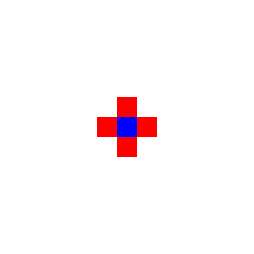
\includegraphics[scale=.4]{ps/gh1.ps} \\ \hline
         \includegraphics[scale=.4]{ps/gh2.ps}      & 
              \includegraphics[scale=.4]{ps/gh3.ps} \\ \hline
     \end{tabular}   
                                                                    \\
   \multicolumn{1}{c}{(a)}  &   &
   \multicolumn{1}{c}{(b)}  &   &
   \multicolumn{1}{c}{(c)}  
     \\
\end{tabular}
} {{\bf Greenberg--Hastings: A Basic CA Excitable Medium}\quad We show
    the state transition graph (a), the ``von Neumann'' neighborhood
    and state variable offsets that this CA uses (b), and four
    consecutive snapshots of the dynamics starting from a plane all in
    the {\em ready} state except a single {\em firing} point in the
    middle (c).}


% The dynamics of our first excitable media rule has the following transition
% function:
% \begin{quote}
%  If {\em ready} and a neighbor is {\em firing}, transition to {\em firing}. \\
%  If {\em firing} transition to {\em resting}.                               \\
%  If {\em resting}, transition to {\em ready}.
% \end{quote}
% As is the case for all cellular automata dynamics, in an update, the
% transition function is applied to all sites simultaneously and the
% next state transition is a function of only the present state.
\smallskip

To familiarize the reader with SIMP scripts we present the full code
for the Greenberg-Hastings automaton and
will dissect it in detail. Just glance over the code---a full explanation
follows.  (Although we make no attempt to provide a full introduction
to the Python language---for that, see the excellent tutorials at
\url{http://python.org}---its clear syntax and semantics should be intuitively
understandable to even the moderately experienced programmer.)

%We'll now present a Python script
%used to obtain the images in \figref{greenberg_hastings}.  
% it's actually just a Python script that uses the SIMP package.) 



% to those familiar with {\tt
% C} or {\tt C++}, object oriented programming, and scripting languages
% with dynamic types.

%\begin{mylisting}
%\begin{alltt}
%{\small
%
\begin{verbatim}
from simp import *            # Import simp and helpers

# ------------------------------------------------ GEOMETRY AND STATE
Y,X = 200,200
initialize(size=[Y,X])        # Declare an YxX square grid
c = Signal(SmallUInt(3))      # State variable (signal) declaration
READY=0; FIRE=1; REST=2;      # Mnemonics for state interpretations

# ------------------------------------------------ DYNAMICS
def gh():                     # Transition-function definition
  if c==READY:
   if (c[-1,0]==FIRE or c[0, 1]==FIRE or # If north,east,south, or west firing.
       c[ 1,0]==FIRE or c[0,-1]==FIRE):  # (Subscripts indicate neigh coord)
      c._ = FIRE              # transition to FIRE
  elif c==FIRE: c._ = REST    # If firing, transition to REST
  elif c==REST: c._ = READY   # If resting, transition to READY

gh_rule = Rule(gh)            # Creates a Rule object for the transition-function.

# ------------------------------------------------ RENDERING
red,green,blue = map(OutSignal,[UInt8]*3)  # Declare the color output signals

def tricolor():               # Function describing an appropriate color map
  if c==READY:
      red._=green._=blue._ = 255 #   READY => white
  elif c==FIRE:
      red._   = 255              #   FIRE  => red
  elif c==REST:
      blue._  = 255              #   REST  => blue

# Package tricolor into a rendering rule with red,green,blue as outputs  
tricolor_rend = Renderer(Rule(tricolor),(red,green,blue)) 

# ------------------------------------------------ INITIALIZE
c[:,:] = READY                 # Initialize all sites to READY
c[Y/2,X/2] = FIRE              # Set site in the center to FIRE

# ------------------------------------------------ USER INTERFACE
ui = Console(tricolor_rend)    # Instantiate a console called "ui"
                               #   and initialize its renderer
ui.bind("STEP",gh_rule)        # Bind the console's STEP event to the update rule
ui.start()                     # Start the interactive interface
\end{verbatim}
%\end{alltt}
%\end{mylisting}
%}
%\end{verbatim}
%}

%After explaining this program in detail we'll be able to extend our
%discussion to more sophisticated techniques with little difficulty 

Many SIMP programs follow the same pattern as
\file{greenberg_hastings.py}.  The script is divided into five
sections: geometry and state, dynamics, rendering, initialization and
user interface.  The very first line in the code imports the SIMP
programming environment from the \module{simp} module. The geometry
and state section first sets up the topology in which the CA will be
defined and declares the CA's state variables. The dynamics section
declares the rule that implements the dynamics.  The rendering section
describes how the state is visulalized.  The initialization section
``sets up the inital state.  The user interface section declares a
\class{Console} object for interactively running the dynamics and
viewing rendering results on-screen.  
% and starts the \class{Console}. 
We'll now address each section in detail.

\subsection{Geometry and State}

Before discussing the geometry and state we address the \code{import}
statement in the very first line. It is a Python statement that
imports \module{simp} and all of its definitions\footnote{Although
SIMP is designed to be used this way rather than as a module imported
with \samp{import simp}, the latter will work, but all \module{simp}
definitions must be qualified as in \code{simp.initialize}.  When
multiple \module{simp} module instances are required, see
\module{import_locally} in \secref{sec:importlocally}.}.
\module{simp} contains various constructs---methods, functions, and
constructors---that the rest of the program uses.  Additionally, it
maintains global variables and defaults used by these constructs.

\medskip

Calling \function{initialize} initializes SIMP's global variables.  In
particular, \var{size} parameter declares the size of the two
dimensional grid where state variables will be allocated.  In the
example, the size is $200\by 200$ and is stored two
variables--\code{Y} and \code{X}--for later use.  In general, the
value of each element declares the size of the grid in that dimension
while the number of elements in the size vector specifies the number
of dimensions.  While \var{size} is the only parameter that SIMP needs
for an ordinary CA, \function{initialize} also has optional
parameters. Among other things, they specify the default lattice
generator matrix and the runtime space-time event processor (STEP)
implemetation to be used. This is discussed further in
\secref{sec:1dsublat} and \secref{sec:initialize}.


\subsubsection{The grid}
\index{grid} \index{coordinates} \index{wrap-around} \index{boundary-conditions}

The grid defines the geometry at the finest granularity.
In two dimensions, one may think of it as a piece of graph paper in
which line intersections are coordinatized sites as shown in
\figref{grid} (a).  The grid is bounded by the \var{size} vector beyond
which it wraps around\fnmark as a torus (\figref{grid} (b,c)).  
%In SIMP, absolute coordinates select sites and rectangular regions containing
%multiple sites. Relative coordinate offset vectors select neighbors in
%local rules and specify shifts performed on objects on the grid.
Other numbers of dimensions generalize directly.

\fntext{Currently, SIMP only supports boundaries that wrap around,
however it is possible to emulate other types of boundaries such as
fixed boundaries (XXX give reference).  In the future, SIMP may
directly support other types of boundaries.}

\Fig{grid}{
   \begin{tabular}{ccc}       
        \includegraphics[scale=.8]{xfig/Grid66.eps}           &
        \includegraphics[scale=1]{xfig/Cylinder.eps}          &
        \includegraphics[scale=.8]{xfig/torus.eps}            \\
%    torus & \multicolumn{3}{c}{points at the edges wrap around} 
       (a) & (b) & (c)
    \end{tabular}
}{{\bf The grid and wrap-around}\quad (a) shows a grid with \emph{size}
(6,6) marks some of its sites (line intersections) with circles and
gives their coordinates. To emulate a boundaryless space, the
coordinates wrap-around with the bottom wrapping to the top (b) and
the left wrapping to the right (c) yielding a torus. Coordinates in
(a) that wrap around at the boundary are shaded gray.}


 
 % SIMP is capable of handling an arbitrary number of dimensions, but
 % most of the time one will be interested in rules in one, two or three.
 % The terminology of this documentation is geared to two dimensions, but
 % objects such as rectangular regions are generally multi-dimensional.
 
 Note that SIMP coordinate vectors are given in order from the most
 significant dimension to the least (ie. $(y,x)$ in two dimensions and
 $(z,y,x)$ in three).  This reflects the positional notation implicit
 in Arabic numbers where the number one hundred and twenty three is
 written from left to right in decreasing order of significance as
 123---more significant digits are appended on the left.  It also
 reflects the storage conventions of \verb|C| and \module{numarray}
 where indices of lower significance are stored closer together.  When
 \verb|C| and \module{numarray} map a multidimensional array to a 1D
 memory array, the unit-stride dimension---the one with the highest
 degree of locality---is the least significant, right-most one.  When
 there is a choice, the programmer should align neighbor access with
 lower dimensions, because, depending on the STEP implementation, doing
 so increases data locality and may make the computation more efficient.  In accordance with
 computer graphics and typographic conventions, for rendering and
 display purposes, X goes to the right, Y goes down and Z goes
 `behind'.
 
 %5 The geometry-and-state section sets up the spatial grid and attaches
 %5 state variables to the sites.  First it uses the \id|geometry|
 %5 declaration method to create a two-dimensional $11$$\times$$11$
 %5 square-grid geometry.  It does this by setting the value of the
 %5 function's predefined \id|size| argument to a list giving the grid
 %5 size in terms of Y and X.  (In general, \id|size| will be much larger
 %5 and may declare a grid with any number of dimensions.)  
 
 
 
 %Before covering each of these sections in detail, we note that
 %some of the variations one can make from this pattern.  The
 %user interface and rendering sections are optional.  Non-interactive
 %programs---such as those that gather statistics or peform long-range
 %experiments---may control the dynamics directly. 
 
\subsubsection{State Declaration}
 
 %We describe the remaining sections in turn.
 % The first imports the SIMP package and initializes a
 % SIMP environment, the next two specify the CA, and the remaining two
 % declare the reneder and 
 % \subsubsection{Geometry and state}
 % by assigning the special variable {\tt SIZE} to a 2-D vector.  Next,
 % the signal {\tt c} (state variable) is declared with three states and
 % variables {\tt READY}, {\tt FIRE}, and {\tt REST} are declared to
 % hold its possible values.  
 
 %\fntext{The \id|context| is a helper module that allows one to access the
 %methods and attributes of an object---in this case, the SIMP
 %environment object---without qualification.}
 
 %\smallskip
 \indexii{{\tt Signal}}{declaration}
 
 SIMP state variables are called {\it signals} and are \class{Signal}
 objects. The line \samp{c = Signal(SmallUInt(3))} allocates a
 signal with a ternary integer state set $\{0,1,2\}$. \var{c} has a
 ternary value at at every point on grid---it's basically a $200\by
 200$ array.  For convenience, the code also creates some mnemonic
 names---\constant{READY}, \constant{FIRE}, and \constant{REST}---for
 each of \var{c}'s possible values.
 
 % When a signal is allocated its default value is zero. 
 
 % \smallskip 
 % Unlike the  taking on values from the set
 % $\{0,1,2\}$.
 %  \id|simp} method for creating one or more state variables on the
 % grid---is called with the keyword argument, \id|c=int_range(3)}, .
 % % Generally, an $n$-state signal takes on values in $\{0,1,\dots,n-1\}$.
 
 % \smallskip 
 % 
 % Before continuing, a few words about Python syntax are in order.  It
 % is easy to discover by inspection that statements begin on new lines,
 % multiple statements on the same line are separated by semicolons,
 % comments begin with `\id|\#}', variables are declared with `\id|=}',
 % list objects are made with square brackets, and function calls use
 % parentheses `\id|()}'; but, the syntax for function declarations is
 % perhaps more obscure.  Functions are declared with the \id|def}
 % keyword and their definitions are contained within indented blocks.
 % Conditional code blocks like those following an \id|if} statement are
 % demarcated by further levels of indentation.  Python's function and
 % conditional block statement syntax is basically a formalization of the
 % C language's informal formatting conventions.  
 % That should be enough for the purposes of this tutorial.  
 % For a complete introduction to the Python language, we refer the
 % reader to the excellent tutorials at \id|python.org}.
 
 % \subsubsection{Transition-function}
 % \smallskip 
 
 % It is not
 % until the \id}rule} object is called that operation is issued.

\subsection{Dynamics} \label{sec:ghdynamics}

\indexii{{\tt Rule}}{declaration}

The dynamics of a CA is defined locally by a transition-function that
is evaluated everywhere in parallel.  In the dynamics section, the
code
\begin{verbatim}
def gh():                     # Transition-function definition
  if c==READY:
   if (c[-1,0]==FIRE or c[0, 1]==FIRE or # If north, east, south,
       c[ 1,0]==FIRE or c[0,-1]==FIRE):  #  or west is firing.
      c._ = FIRE              # Transition to FIRE
  elif c==FIRE: c._ = REST    # If firing transition to REST
  elif c==REST: c._ = READY   # If resting transition to READY
\end{verbatim}
defines the transition-function for the Greenberg--Hastings rule.  The
statement \samp{gh_step = Rule(gh)} uses the 
transition-function \code{gh}---which is just an ordinary
Python function---to create a parallel CA \class{Rule} object that,
%  by packaging \id}gh} into a \id|Rule| object.  
when called (as in \code{gh_step()}), applies the transition-function
to all sites on the grid in parallel.  


A \class{Rule} object packages a transition-function into a STEP
operation---an object that a back-end STEP implementation can execute.
The object itself describes the operation---the transition-function,
the context in which it was created etc.---while calling it tells the
back-end to execute the operation.  A SIMP program may use a
\class{Rule} object directly by calling it to execute the transition
function or it may pass it as an argument to other constructs, such as
the\class{Console} and the \class{Renderer}, that may need it.  A
\class{Rule} is not the only type of STEP operation---\class{Shift},
\class{Sequence} and \class{Shuffle} are other examples that appear
later in this tutorial and in \secref{sec:stepops} of reference
manual.  In the early sections of this tutorial, we'll just be
discussing the basic behavior of \class{Rule} objects---in later
sections such as \secref{sec:rule} and \label{sec:sublatandrules}
we'll address advanced topics such as frozen context variables, 
transition-function parameterization, and shifting.

% Under the hood, the STEP runtime prepares implementation-dependent
% structures---such as compiled code loops and lookup tables---for
% executing the rule.

\medskip 

Now, a transition-function locally maps current-state input values to
next-state output values.  Inside a transition-function, signals are
accessed locally, therefore, rather of referring to the entire
parallel data allocation, as is normally the case, accessing a signal
name inside a transition-function references its value \emph{at the
site being updated}.  For example, to check whether \var{c} at the site
being updated is currently in the \constant{READY} state, the 
transition-function uses \code{c==READY}.  To write the output value of a signal, a
transition-function assigns values to a signal's output
attribute---the underscore attribute.  For example, to set the the
next state value of \var{c} at the site being updated to \emph{firing} the
transition-function makes the assignment \samp{c._ = FIRE}.

\function{gh} looks at the {\em von Neumann neighborhood} of
\var{c}---the site itself and its neighbors at an offset of $\pm 1$ in
the $Y$ and $X$ directions as shown in \figref{greenberghastings} (b).
The neighbor value of \var{c} to the right is \code{c[0,1]}, to the
left is \code{c[0,-1]}, above is \code{c[-1,0]}, and below is
\code{c[1,0]}.  SIMP subscripts are listed from the most significant
to the least\fnmark; therefore the subscript in the higher dimension,
Y, comes before that of the lower dimension, X.  In accordance with
the conventions of computer graphics---Y grows downwards while X grows
rightwards (Z grows away from the viewer).  
\begin{note}
Within a transition-function, neighbor values are referenced by
relative subscripts.  Outside of transition-functions, subscripts are
absolute coordinates.
\end{note}


\fntext{As of version 0.6 this convention replaces the prior
least-significant-first convention inherited from physics and linear
algebra.  Although the change was precipitated by the adoption of the
{\tt numarray} package for handling multidimensional arrays in Python,
the most-significant-first convention is more natural when subscripts
are interpreted as a generalization of positional notation for
numbers---subscripts, like digits, are usually ordered from the most
significant to the least.}

%\subsubsection{Comments and restrictions on rules and transition functions}

\function{gh} does not always assign an output value of \var{c}. For
example, if the current state is \emph{ready} and no neighbors are
firing, the rule does not write a next state value.  What, then is the
next state value of \var{c}?  Of many conceivable defaults, our choice
in SIMP was that the default new value of \code{c} is the previous
value of itself.  Thus, the rule specifies that if no neighbors are
\emph{firing} and \var{c} is \emph{ready} then \var{c} remains
\emph{ready}.

\subsection{Rendering}

% from a computer engineering perspective where
%  indexing conventions, X is given before Y and
% the X subscript grows rightwards while the Y subscript grows
% downwards. 
%  In general, index elements are given from left to right in increasing order of significance.
%Following the conventions of computer graphics, X increases to the
%right and Y increases down.  

% \subsubsection{Rendering}
%\smallskip 

\index{OutSignal}
The rendering section declares how to convert state information into
images that can be displayed.  Like the dynamics, rendering behavior
is defined by a \class{Rule}.  Unlike the dynamics, however, the
\class{Rule} does not output to ordinary signals. Instead, it writes to
special \class{OutSignal} objects---they are just like
\class{Signal} objects, except that they are write-only.  SIMP also
supplies special \class{Renderer} classes to manage the conversion and
output of rendering data to image arrays.  The \class{Renderer}
provides an interface that's suitable for on-screen display by a
\class{Console} user interface.

The output of a rendering rule is an array containing color
information.  Color channels are encoded with 8-bit color
\class{OutSignal} objects of type \class{UInt8} (8-bit unsigned
integer).  The \class{UInt8} type is necessary because the \class{Console}
expects images encoded as 8-bit values in which 0 is the minimum
intensity and $255$ is the maximum intensity.  Conceptually, the 
simplest way to declare the necessary \class{OutSignal} objects
for color rendering is as follows
\begin{verbatim}
red = OutSignal(UInt8)
green = OutSignal(UInt8)
blue = OutSignal(UInt8)
\end{verbatim}
However, we use the following more succinct form
\begin{verbatim}
red,green,blue = map(Signal,[UInt8]*3)
\end{verbatim}
The code \code{[UInt8]*3} is Python shorthand for
\code{[UInt8,UInt8,UInt8]}, a list with three references to the
\code{UInt8} type. The \function{map} is a builtin Python function
that, in this example, calls the \class{OutSignal} constructor on each
of the three list elements and returns a list with three new \class{OutSignal}
objects. Finally, Python list comprehension handles the assignment of
\code{red,green,blue} to the three signals returned by \function{map}.
In this example, and many others, mastering Python helps one to master
SIMP. 

% Although one may directly declare \class{OutSignal} objects
% with the \class{OutSignal} class, SIMP provides a special function
% called \function{declarecolors} which is basically a macro-like
% function that automatically declares the commonly used
% channels---\var{red}, \var{green}, \var{blue}, \var{white}, and
% \var{alpha}---in the global namespace.  (\var{white} is for grayscale
% rendering and \var{alpha} is for opacity in three--dimensional
% rendering.)  Instead writing a statement like \samp{red
% = OutSignal(UInt8)} for each color channel, one can instead 
% call \function{declarecolors}.

\index{rendering}
The rendering function was declared as 
\begin{verbatim}
def tricolor():               # Function giving a color mapping
  if    c==READY:
      red._=green._=blue._ = 255 #   READY => white
  if    c==FIRE:
      red._   = 255              #   FIRE  => red
  elif  c==REST:
      blue._  = 255              #   REST  => blue
\end{verbatim}
Similar to the rule's transition-function, the rendering function 
takes advantage of default values.  This time, it takes advantage of the
fact that the default value of an \class{OutSignal} is $0$. Therefore, 
when \samp{c==FIRE}, \code{red} is set to \code{255} while \code{green} and 
\code{blue} have a value of \code{0}. 

% This is because the renderer images
% can be either grayscale in which case the only channel is \id{white}
% or they can have RGB color in which case the color channels are
% \id{red}, \id{green}, and \id{blue}.
\indexii{declarecolors}{example}
After declaring the color-map function the program creates a \class{Renderer} 
object as follows
\begin{verbatim}
tricolor_rend = Renderer(Rule(tricolor),(red,green,blue))
\end{verbatim}
The first parameter is the rendering rule, the second is the set of
outputs that are rendered.  The tuple \samp{(red,green,blue)} gives the 
ordering of the output signals in the array that results from the rendering
operation.  We give them in this order because the \class{Console} expects
RGB arrays. 

% Notice that in this code, rather
% than using the \var{white} channel to write a white output when
% \samp{c==READY}, the function assigns the RGB values.  
% This is because \var{white} is intended for use in \var{grayscale}
% mode when, instead of rendering to three color channels, we render to
% a single channel that encodes intensity.  For grayscale rendering,
% \function{declarecolors} also declares the tuple
% \samp{grayscale=(white,)} so that the renderer may render grayscale
% images from rules that only set the \var{white} intensity value. For
% an example of grayscale rendering, see \secref{sec:xtrender}.


%  section, the
% rendering section defines a parallel operation by passing a local
% function to a constructor.  This time, the parallel operation is
% \id{render} and it is used to construct the \id{rend} object.  The
% \id{tricolor} function indicates how signal values should be rendered
% to the \id{red}, \id{green}, and \id{blue} color channels of a pixel.
% Color channel values range from no color at 0.0 (the default) to
% saturation at 1.0. A special color channel called \id{gray} sets the
% value of \id{red}, \id{green} and \id{blue} simultaneously.  For
% three-dimensional rendering, the \id{alpha} channel determines
% opacity.



%The run section is a relatively straightforward script that
%initializes the state and runs several updates, rendering each one to
%an image.  The first initialization statement uses Python slice
%indexing to set all sites to {\em ready}, while the second sets a
%single site in the center to firing.  Here the subscripts indicate
%{\em absolute} coordinates, not offsets.  

\subsection{Initialization}

This section uses signal subscripts to assign initial values to the signals.  
As previously mentioned, the subscripts here are global. 
\begin{verbatim}
c[:,:] = READY                 # Initialize all sites to READY
c[Y/2,X/2] = FIRE              # Set site in the center to FIRE
\end{verbatim}
The first statement uses Python/\module{numarray}-style
multidimensional slicing to assign all states to \emph{ready}.  The
second sets a single site in the center to firing.

One may also read out signal values using subscripts.  For example, 
\begin{verbatim}
a = c[0,5].value() 
\end{verbatim}
reads out the scalar integer value at coordinates $(0,5)$.  We must
call the \method{value} method to read the actual value at
\code{c[0,5]}.  This is because subscripting a signal actually returns
a \class{SignalRegion} object referring to a specific region of a
signal, rather than the value itself.  If one writes \samp{a =
c[0,5]}, then \code{a} is a \code{SignalRegion}.  To get the actual
value, one must use \method{a.value()} to dereference the
\class{SignalRegion}; conceptually, a \class{SignalRegion} is similar
to an address (pointer) in a language like {\tt C}.  In contrast to
reading values, is not necessary to explicitly dereference a
\class{SignalRegion} when writing values using subscript assignment
(as in \samp{c[:,:] = READY}), because Python provides special hooks
for handling subscript assignment\fnmark.

\fntext{Subscript assignment only works when a subscript expression
appears on the left-hand side of an assignment. Given a named
\class{SignalRegion} obtained with code like \samp{a = c[0,5]}, one
must instead write the value there using the assignment attribute as
in \code{a._ = 2}.}

Because a \class{SignalRegion} refers to an area, rather than a
specific value, it can be used in a variety of more general contexts,
such as making named neighbors and constructing \class{Read} and
\class{Write} operations.
% , where a signal location,rather than a value, is needed. 
Note, however, that inside of a rule's transition-function, where only
the value is of interest, one does not use the \method{value} method;
this is because subscripting in that context automatically returns the
value.

One can also use subscripting to read out arrays of values; for
example, to read out the $5\by 5$ array of values from $(0,0)$ up
through but not including $(5,5)$ one, would use
\begin{verbatim}
arr = c[0:5,0:5].value()
\end{verbatim}
The array returned is a \class{NumArray} object.  One can also 
assign slices using array values 
\begin{verbatim}
c[15:20,10:15] = c[0:5,0:5].value()
\end{verbatim}
Note that the \class{NumArray} need not have come from a \class{Signal}; it
could just as well have come from a file or have been constructed
on-the-fly (as in \code{numarray.zeros((5,5))}).  

To read the entire array, one can use a statement like
\begin{verbatim}
arr = c[:,:].value()
\end{verbatim}
Note that if the signal region refers to a single site, \method{value()} 
returns scalar element and if it refers to multiple sites, \method{value()} 
returns an array.
 

SIMP uses the \module{numarray} module extensively for representing
and manipulating \class{Signal} data.
%For convenience one may use lists (lists, tuples, and lists of lists) 
% in place of actual \class{NumArray} objects and SIMP will convert them to
% \class{NumArray}s when necessary.
The \module{numarray} module and classes provide full Python support
for multidimensional arrays.  This support includes utilities for
generating arrays, saving them to files, and performing all kinds of
transformations and analyses.  

A \class{NumArray} object can be saved to a file in a variety of
ways. One way is to use the Python \module{pickle} module.
\begin{verbatim}
import pickle
pickle.dump(arr,open("state_file","wb")) # dump the array to "state_file"
\end{verbatim}
To read the file back, use 
\begin{verbatim}
arr = pickle.load(open("state_file"))
\end{verbatim}
Another option is to use the \method{tofile} method of the
array. Certainly, there are many other ways as well.  While we mention
some of the useful \module{numarray} package features in this
tutorial, one should see the Numarray documentation available at
\url{http://www.stsci.edu/resources/software_hardware/numarray} for
full details. SIMP also defines some additional helper numarray
functions such as \function{makedist}, \function{getdist},
\function{arraytopnm}, \function{magnify2d}; see
\secref{sec:imgarrayhelper} and \secref{sec:numarrayhelper} for
details.


\subsection{User Interface}

% ---instead of whichever site is being updated.  is a slice
% containing all points, while \id{c[4:7,3:9]} is a slice containing a
% $3\by 5$ rectangle starting at \id|[4,3]} and extending through
% \id{[6,8]}.

%\smallskip

% {\bf The console user-interface} 
% \smallskip

%  \displays rendering results and provides keypress commands
%  \to allow the user to step through updates, run a series of steps,
%  \change configurations, and invoke user defined functions. 

All of the example SIMP programs instantiate a \class{Console} object
to perform on-screen rendering and provide an interactive
user interface.  In the current example, the code for declaring and
initializing a \class{Console} is
\begin{verbatim}
ui = Console(tricolor_rend)    # Instantiate a console called "ui"
                               #   and initialize its renderer
ui.bind("STEP",gh_rule)        # Bind the console console's STEP event to the update rule
ui.start()                     # Start the interactive interface
\end{verbatim}
The first line creates a \class{Console} object called \code{ui} and
brings up an on-screen viewer using \code{tricolor_rend}, the renderer
previously defined.  Because \code{tricolor_rend} implements the
\class{Renderer} interface, the the \class{Console} knows how to use
it to generate rendered image arrays and to control the region that is
rendered.

The \class{Console} \method{bind} method is used to bind custom
commands to keypress events.  For example, to re-initialize the CA
state when \kbd{S} is pressed,
\begin{mylisting}
\begin{alltt}
def seed():
    "Initialize all sites to READY with a FIREING site in the center"
    c[:,:] = READY          # Set all sites to READY
    c[Y/2,X/2] = FIRE       # Set the center site to FIRE
ui.bind("S",seed)           # Bind 'seed' to key "S"
\end{alltt}
\end{mylisting}
Lower-case keys are reserved for predefined commands; user-defined
commands should be bound to upper case keys.  Brief documentation
derived from the documentation strings of bound commands is printed
when the user presses the help key, \kbd{h}.  For this reason, it is a
good idea to define a documentation string as is done above.

[XXX explain numeric arguments] 

In the code, \samp{ui.bind("STEP",gh_rule)}, binds \code{gh_rule} to a
special event called a \samp{STEP} event.  A \samp{STEP} event
triggers an update of the dynamics.  The console handles them by
calling \code{gh_rule} and invoking the \code{renderer} to display the
result on-screen.  Pressing \kbd{Space} generates a single \samp{STEP}
event, while pressing \kbd{Enter} causes them to be scheduled
repeatedly until this behavior is turned off by pressing \kbd{Space}. 

Finally, calling \code{ui.start()} starts the
interactive interface, and does not return until the user quits by
pressing \kbd{q}.


\subsubsection{Scripting}

\indexii{arraytopnm}{example}
\index{ppm file}
One need not define an interactive user interface if the program is meant 
to run in script mode.  For example, the following code runs several 
iterations and generates a sequence of portable pixmap (\file{.ppm}) images 
like the ones shown in \figref{greenberghastings} (c)
\begin{verbatim}
for i in range(4):
    img_arr = tricolor_rend() # get an array containing the current state
    open("gh%i.ppm" % i,"wb").write(arraytopnm(img_arr)) # save to file
    gh_rule() # do a step of the dynamics
\end{verbatim}
Calling a renderer object returns the contents of the renderer's
current view (of course, the renderer has methods for changing the
view; see \secref{sec:renderer}).  Normally, arrays returned by a
renderer are three-dimensional numarrays indexed by Y,X, and the color
outputs. (If \emph{grayscale} rendering is used, they will simply be
two-dimensional arrays.) The SIMP helper function
\function{arraytopnm} converts such arrays to \file{.ppm} formatted
strings, which is a handy because the format is easy to read and write
and can be converted to many other formats using Jef Poskanzer's
widely available {\tt netpbm} \index{netpbm} library and command-line
tools.

One may also drive the \class{Console} from a script.  For example, to 
display a sequence of four updates on-screen before starting the console, 
one could use the code
\begin{verbatim}
for i in range(4):
    ui.issue(" ")# issue a space character, which causes a single 
                 # STEP to be run and rendered as if the user pressed space.
ui.start() # begin running the console  
\end{verbatim}

% ----------------------------------------------------------------
              \section{A stochastic excitable-medium CA} \label{sec:stochastic}
% ----------------------------------------------------------------

Now that we have seen how to program a simple CA and have a basic idea
of how the SIMP environment works, let's consider a randomized
(stochastic) version of the Greenberg--Hastings rule, where state
transitions occur probabilistically.  We'll show how to program it
efficiently with SIMP and how to gather statistics about the dynamics.
The new rule statement is:
\begin{quote}
    Transition to {\em firing} with probability $p$ if {\em ready} 
    and a neighbor is {\em firing}; transition to {\em resting} with 
    probability $q$ if {\em firing}; and transition to
    {\em ready} with probability $r$ if {\em resting}.
\end{quote}

% Belousov-Zhabotinskii reaction 
We can interpret this dynamics as a model of a prairie fire---a {\em
ready} site `has grass', a {\em firing} site is one that's `on fire',
and a {\em resting} site is `burned out'.  The transition
probabilities $p$, $q$, and $r$ give the flammability, burn rate, and
regrowth rate.  The Poisson statistics of the transitions have an
average ignition, burning, and regrowth time of $1/p$, $1/q$, and
$1/r$. By modulating $p$, $q$, and $r$ one arrives at different
dynamics as discussed and demonstrated in \figref{excitabledynamics}.

% Generally speaking, when the flammability of the grass is high---$p$
% is close to 1---the fire spreads quickly, giving rise to a wave-front
% like that of the deterministic model. When it is low---$p$ is close to
% 0---the fire spreads slowly and will likely burn out if the burn rate
% is not low.  When the flammability is not significantly lower than the
% burn rate, a spark will catch and burn all grass available to it.  If
% the regrowth rate is non-zero, it will sustain waves of fire that
% oscillate through the space---the higher the regrowth rate, the closer
% the waves will be to each other.  

\Fig{excitabledynamics}{

\begin{tabular}{m{.8in}m{1in}m{3.0in}}
   {\small
     \begin{tabular}{c}   
         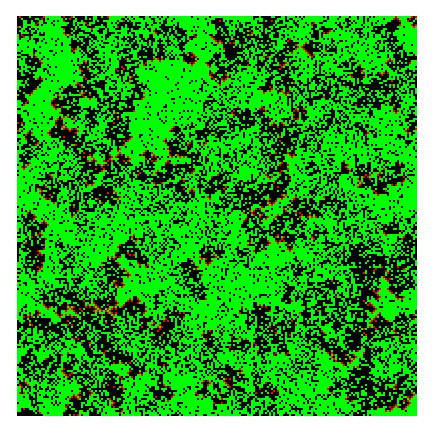
\includegraphics[scale=.3]{ps/P70Q100R6.ps} \\ 
                   $(.7,1,.06)$                        \\
         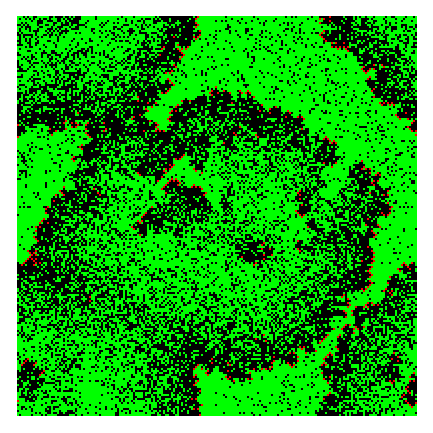
\includegraphics[scale=.3]{ps/P70Q100R3.ps}\\
                   $(.7,1,.03)$                        \\
     \end{tabular}  }
   & 
   {\small
     \begin{tabular}{c}   
         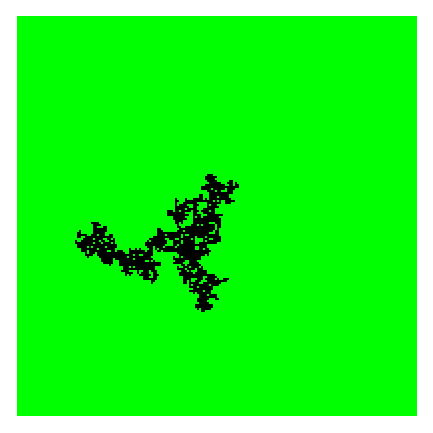
\includegraphics[scale=.3]{ps/P50Q100R0.ps} \\ 
                      $(.51,1,0)$                     \\
         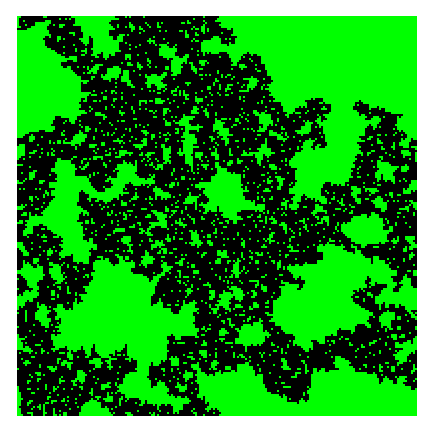
\includegraphics[scale=.3]{ps/P54Q100R0.ps} \\ 
                      $(.54,1,0)$                     \\
     \end{tabular}   }
   &  
    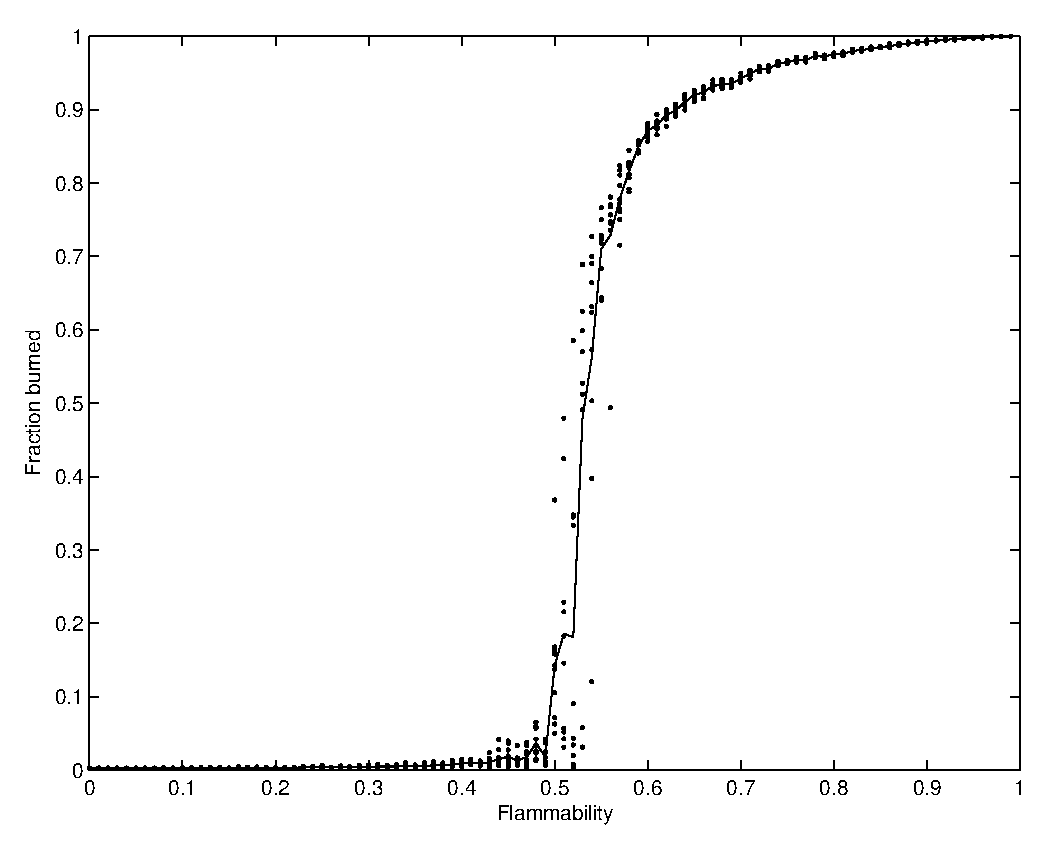
\includegraphics[scale=.4]{ps/fireplot.eps}
%    \\
%    \multicolumn{1}{c}{(a)}  &    
%    \multicolumn{1}{c}{(b)}  
     \\
\end{tabular}
} { {\bf Stochastic Greenberg--Hastings Parameter Space}\quad On the
 left we show several snapshots of the system taken at different
 points in the $(p,q,r)$ parameter space.  When the flammability $p$
 is high and the regrowth rate $r$ is low, as in $(.7,1,.03)$ and
 $(.7,1,.06)$, sustained waves form and endlessly propagate over the
 toroidal space---in a way it is similar to the Belousov--Zhabotinsky
 chemical reaction.  Notice that the regrowth rate affects the
 wavelength.  When the regrowth rate is zero, as in $(.51,1,0)$ and
 $(.54,1,0)$, a `forest-fire' situation arises where the vegetation
 does not have time to grow back.  The amount of forest burned depends
 critically upon the flammability parameter as evidenced by the amount
 burned in the two figures.  On the right, we have used SIMP to
 perform a kind of percolation experiment in which we show the
 fraction of forest burned by a single spark over ten trials as a
 function of the flammability coefficient.  Dots indicate the fraction
 burned on each trial, and the solid line marks the average over the
 trials. }

\smallskip
Implementing the new dynamics in SIMP amounts to adding stochastic
transitions to the basic rule.  We'll create three signals---\code{P},
\code{Q}, and \code{R}---as binary random variables with the desired
distribution---Pr(\code{P}=1)=$p$, Pr(\code{Q}=1)=$q$, and
Pr(\code{R}=1)=$r$.  We'll use these signals as `unfair coin tosses'
when deciding whether to take a transition---if a signal's value is
\code{1} the transition will be taken, otherwise it will not. The new
signal declarations\fnmark are
\begin{mylisting}
\begin{alltt}
binary = SmallUInt(2)          # Binary state variable type with values in {0,1}
P,Q,R = map(Signal,[binary]*3) # Declare the three random state variable signals
\end{alltt}
\end{mylisting}

\fntext{Note, we could just as easily have declared these signals as 
 {\tt P,Q,R = map(Signal,[SmallUInt(2)]*3)} but we chose to demonstrate the 
use of a type object.} 

The modified rule is
\begin{mylisting}
\begin{alltt}
def stochastic_gh():
   if   c==READY and P==1:
     if (c[-1,0]==FIRE or c[0, 1]==FIRE or 
         c[ 1,0]==FIRE or c[0,-1]==FIRE):  
       c._ = FIRE                            # Stochastic transition to FIRE
   elif c==FIRE and Q==1: c._ = REST         # Stochastic transition to REST
   elif c==REST and R==1: c._ = READY        # Stochastic transition to READY
\end{alltt}
\end{mylisting}
We have not explained yet how \code{P}, \code{Q}, and \code{R} implement
the desired random distributions.  The most direct way is to use a
random number generator to assign random values to the signals so as
to fulfill the desired distribution.  SIMP provides
\function{makedist} to do this.  The function takes two
arguments---the shape of the output array and the distribution of
values.  For example, within the {\tt set_parameters} function of the 
{\tt stochastic_greenberg_hastings.py} code, the line
\index{\function{makedist}}
\begin{mylisting}
%Randomize(P=[1.-p,p])
\begin{alltt}
P[:,:]  = makedist(P.shape,[1-p, p])
\end{alltt}
\end{mylisting}
assigns the values of \code{P} to a newly generated random array with
the same shape as \code{P} and having values of 0 and 1 distributed
independently with probability $(1-p)$ and $p$; similar code sets the 
distributions for \code{Q} and \code{R}.   (Note that distributions need not be 
normalized to one---a distribution parameter of \code{[3,4]} 
would create an array with a 3 to 4 ratio of zeros to ones.)

Although this strategy of generating distributions works, it requires
an expensive call to a random generator {\em for each array element}.
Regenerating distributions in this way before {\em each step} would slow
computations considerably.  Fortunately, there is a less expensive way.
Because our rule can not `see' long-range correlations---local
information tends not to travel too far before `diffusing'---we can
{\em regenerate} the local random variables by {\em shuffling} them.
By rearranging the same data in a non-local way---say, by shifting a
\class{Signal} by a random amount\footnote{This is the policy that the
current STEP implementations employ under the hood. The ideal shuffle
is a random permutation, however, a true random permutation is
expensive to implement.  In the future STEP implementations may make
more sophisticated, but still inexpensive, implementations of
\code{Shuffle} available.}---we can cheaply ``recharge'' the patch of
randomness that a locale sees.  It's like a shell game in which a
sequence of small patches from a much larger space are revealed
randomly, and unless the dynamics is an especially `smart' adversary
tuned to our game it will not be able to tell that the patches it is
shown come from our cheaper source of shuffled randomness.

\index{\class{Shuffle}}
To shuffle the distribution before each update, we use the \class{Shuffle}
operation and create an update \class{Sequence} that shuffles the random
signals before calling the stochastic rule.
\begin{mylisting}
\begin{alltt}
stochastic_gh_step = Sequence([Shuffle([P,Q,R]),
                               Rule(stochastic_gh)])
\end{alltt}
\end{mylisting}
We have introduced two new STEP operations---\class{Shuffle}, which we
just explained and \class{Sequence}. A \class{Sequence} is not really
an operation in itself, but an ordered sequence of STEP operations.
In addition to being a useful programming construct, a
\class{Sequence} informs the STEP about sequences of operations that
will be called together.  A STEP may then optimize such a sequence.

% By default, SIMP's randomness generation
% facilities---including those used to control Shufflering---are seeded to
% the current system-time; but, explicit integer seeds for the
% repeatable generation of randomness may be set via the \id{seed_rng}
% method.

Finally, we outline the methods\fnmark used to obtain the data plotted in
\figref{excitabledynamics}.  The data was gathered by running an outer
loop that iterated over the $p$ values in increments of $.01$ from $0$
to $1$.  For each value, ten trials were run.  At the beginning of
each set of trials, a randomized assignment was used to load a new
distribution corresponding to the new value of $p$ into \code{P}.  At
the beginning of an individual trial, \code{c} was initialized to all
{\em ready} except for a single {\em firing} spark in the center.
Next, an inner loop repeatedly invoked
\function{stochastic_gh_step()}, checking every tenth step to
determine whether `the fire had burned out' by examing the
distribution of states returned by \samp{dist = getdist(c[:,:].value(),0,3)}.
\function{getdist} is a SIMP helper function that, given an array and
a range of integer values, returns a histogram vector giving, for all
values in the range 0--3, the number of sites having that value.  Once
it was determined that the fire had burned out, the fraction burned
was computed from \code{dist}. 

\fntext{XXX The actual code for generating the plot is not yet in the 
        examples distribution.}

% These concepts are made precise in my personal notes and will be 
% addressed in my thesis.

% Note, one could use the Smith random number generator for the case where
% the update rule draws values from the distribution in a disjoint fashion.
% That is, depending on values of the state, different distributions are 
% sampled.  Automated techniques for recognizing this situation at the 
% compilation stage could be created.  Doing so would require that random
% variables be declared as a special type of signal.  It might also 
% require their distribution to be constant, which would be a drawback
% in parameterized experiment.  The advantage of using a Smith random number
% generator is that fewer bits might be needed.  Indeed, I believe that 
% it is just log(N) where N is the number of disjoint values.  Notice, however,
% that uncorrelated variables are harder to generate and would generally
% require N bits if they are sampled simultaneously.

% Sample code using builtin random number generators...
%  P  = NewRandomSignal(2)
%  Q  = NewRandomSignal(2)
%  R  = NewRandomSignal(2)
% 
%  P[:,:] = {0:1.-p, 1:p}
%  Q[:,:] = {0:1.-q, 1:q}
%  R[:,:] = {0:1.-r, 1:r}
% 
%  And this is it...the signals would automatically be Shufflered before 
%  they are sampled.  This may be be bad because it separates the user
%  from the reality of how the random number is generated and how
%  effective it could be expected to be.


% ----------------------------------------------------------------
 \section{A one-dimensional CA and space-time renderer} \label{sec:xtrender}
% ----------------------------------------------------------------
One-dimensional systems are usally rendered using space-time diagrams
in which the history of several consecutive states is displayed as a
two-dimensional image, with the horizontal axis representing space and
the vertical representing time.  The \class{XTRenderer} provides
special support for space-time rendering.  We present a simple CA
called {\sc Parity} as an example. We define it on a one-dimensional
lattice with binary signals.  The transition-function adds the left,
right, and center values and yields 1 if the sum is odd or 0
if the sum is even.
% --------------------------------
       \subsection{The program}
% --------------------------------

The code for the {\sc Parity} dynamics is 
\begin{verbatim}
from simp import *
X=50
initialize(size=[X])    # 1D grid
# -------------------------------- SIGNAL DECLARATION
c = Signal(SmallUInt(2))  # binary state
# -------------------------------- TRANSITION FUNCTION
l,r = c[-1],c[1]  # declare the neighbor directions
def parity(): 
    c._ = l^c^r  # ^ denotes 'xor', sets bit if 'l+c+r' is odd.
parity = Rule(parity)    
\end{verbatim}
The code declares \code{l} and \code{r} to represent \code{c[-1]} and
\code{c[1]} (left and right)---although \code{c[-1]} and \code{c[1]}
could instead have been used in the transition-function we wanted to
demonstrate the use of named \class{SignalRegion} objects.  The code
below declares a space-time renderer, initializes the state to zero
with a single one point in the middle, and creates a console.
\begin{verbatim}
# -------------------------------- RENDERING
white = OutSignal(UInt8)
def bw():
    if not c: white._ = 255
bw_xt = XTRenderer(Rule(bw),white,time=X/2)
# -------------------------------- INITIALIZE
c[X/2]=1  # point seed in the center.
# -------------------------------- CONSOLE
ui = Console(bw_xt,mag=8) # set the renderer and the default magnification
ui.bind('STEP',parity) # Specifies the 1D renderer.
ui.start()
\end{verbatim}
Rather than employing the usual renderer, we employ a
\class{XTRenderer} to capture the space-time history of the CA. An
\class{XTRenderer} object defines a special method called
\method{record} for capturing the space-time diagram over a sequence
of time steps. Every time the \class{Console} does a \code{STEP}, it
looks for and automatically calls a renderer's \method{record} method
if it's defined.  The image in \figref{parityxt} depicts a space-time
diagram generated by the console.  Space runs horizontally while time
runs vertically. The window of time recorded by the \class{XTRenderer}
is set with the \var{time} parameter. In this diagram, time increases
downwards.  By using a negative value for \var{time} one can make time
increase going upwards.

\Fig{parityxt}{
\begin{tabular}{c}
  \includegraphics[scale=.8]{simpppm/parity1d.ps} \\
\end{tabular}
} { {\bf 1D Parity CA space-time diagram}\quad Initalized with a single point
in the center and updated 24 times. }

In the example, the magnification was set to 8 using the \var{mag}
parameter of the \class{Console}. (Grid lines were drawn because the
magnification was high; to turn these lines off, set the
\var{showgrid} \class{Console} constructor parameter to zero.)  The
image was collected interactively using the \function{CaptureView}
command (\kbd{c}), but could have ben captured using the script
discussed below.

% XXX document the LutRule for enumerating Wolfram-like CA
% --------------------------------
   \subsection{Using a script to record the history} 
% --------------------------------

Instead of using the console, one might capture the image of \figref{parityxt}
using a script
\begin{verbatim}
bw_xt.record()   # Record the initial state
for i in xrange(24): # Do 24 updates
   parity() # call the rule (does a step of the dynamics)
   bw_xt.record() # record the state
arr = bw_xt()  # get the output array 
rescaled_arr = magnify2d(arr,mag=8,grid=1) # magnify with grid lines
open("out.ppm","wb").write(arraytopnm(rescaled_arr)) # output image file
\end{verbatim}
First it records the initial state, then it runs the dynamics 24
times, calling the \method{record} method of the \class{XTRenderer}
after each update. Next, using \method{magnify2d}, it gets the output
array, magnifies it, and adds grid lines. Finally, it converts the
array to a \file{.ppm} string and saves it to the file, \file{out.ppm}.


% ----------------------------------------------------------------
\section{Discussion: \class{Rule} transition-functions}
\label{sec:rule}
% ----------------------------------------------------------------


% \begin{note}
% More precisely, the default next-state value for a signal is its
% previous value \emph{if and only if} that signal appears as an input.
% Otherwise, the default output value is \emph{zero}.  This behavior ensures
% that extra inputs to the rule are not generated in the case that a
% signal is only written. If this were not the default behavior, all
% outputs would also be required to be made into inputs, which would be
% bad since the cost of evaluating a transition function is exponential
% in the number of inputs when a lookup table is used to implement the
% function.  (This behavior applies only to signals that appear as
% outputs.  The values of signals that do not actually appear as outputs
% of a rule are not changed.)
% \end{note}
%This is because the
%default next state value is the current state.  With this
%understanding, 
% \begin{warning}
% This default behavior \emph{only} occurs when an output is also used
% as an input. If it is not, the default output value is zero. 
% \end{warning}

A \class{Rule}'s transition-function specifies the local function
that's evaluated in parallel at every point of the \class{Rule}'s
lattice when the \class{Rule} is called.  For the most part, a
transition-function has the same syntax and semantics as an ordinary
Python function.  However, for convenience and to allow a STEP to
implement a \class{Rule} efficiently (for example, by transforming it
into a lookup table or {\tt C} code), a transition-function has some
special behaviors and restrictions not present in ordinary Python
code.  This section discusses these aspects of transition-functions. 

\subsection{The basics}

The transition-function is a local function that computes next-state
signal values from their present-state values.  It reads present-state
values from a signal directly and writes next-state values to a signal
using thhe underscore attribute.  Inside the transition-function,
subscripts are relative to the site being updated; outside they are
relative to the origin.

As an example, consider a two-dimensional program with 
a \class{Signal}, \code{c}.  Inside a transition-function, the 
subscripted signal \code{c[0,0]} gets the value of \code{c} at an 
offset of zero from the site being updated.  The next-state 
value of a signal is written using the underscore attribute, as in \code{c[0,0]._=1}.
For example, in the following 2D parity rule, we can write
\begin{verbatim}
c = Signal(SmallUInt(2))
def parity():
   c[0,0]._ = c[0,0]^c[-1,0]^c[0,1]^c[1,0]^c[0,-1] # center,North,East,South,West
parity_rule = Rule(parity)
\end{verbatim}
in which next-state value is the binary exclusive-or of the signal and its 
nearest neighbors.

\subsubsection{Implicit zero offset}
Most transition-functions access the signal at an offset of zero. 
Therefore, as a convenience, when a signal is accessed in a 
transition-function without as subscript the implicit subscript is zero.  
So, within a transition-function, \code{c} is equivalent to \code{c[0,0]} and
\code{parity} may be rewritten as 
\begin{verbatim}
def parity():
   c._ = c^c[-1,0]^c[0,1]^c[1,0]^c[0,-1]
\end{verbatim}
In contrast, outside of a transition-function, \class{c} refers to 
the values at all sites and \code{c.value()} returns the entire 
array of values in \code{c}. 

\subsubsection{The present-state and next-state are independent values}
In a transition-function, the present-state of a signal remains 
unchanged even after the next-state value is assigned.  
Therefore, even if we write
\begin{verbatim}
def example():
   c._ = 1
   if c==0: # may still be true
      ....
\end{verbatim}
the \code{if} conditional may still be true since \samp{c._ = 1} assigns
the next-state, but \code{c==0} references the present-state. 

\subsubsection{Signal references are variables}
Inside a transition-function, present-state and next-state signal references
are variables. This stands in contrast to the ordinary context 
in which \class{Signal} and \class{SignalRegion} objects behave like addresses 
and must be explicitly dereferenced by calling the \method{value} method.  

For example, in a transition-function like
\begin{verbatim}
def example():
   ne = c[-1,1]
   ne._ = 1
\end{verbatim}
an error would be raised because \code{ne} (short for Northeast) is a 
variable that holds the Northeast \emph{value} of \code{c} at an offset of \code{[-1,1]}  rather than a \emph{reference} to this location. When a neighbor 
reference is needed, the proper way to get it is outside of the transition-function as in
\begin{verbatim}
ne = c[-1,1]
def example():
   ne._ = 1
\end{verbatim}
The transition-function should only access output values using global names.

%The transition function accesses signals by name using names 
%appearing in the global namespace.  

% This is because the code analysis also does not currently perform the 
% dynamic type analysis necessary to follow the assignment of signals to 
% alternate local names.  Therefore, a statement like \samp{a = c; a._=1} 
% inside of a transition function would fail.

\subsection{Frozen global context}  

The \emph{global context} of a function is the set of global values it
references.  The global context of a \class{Rule}'s
transition-function is frozen when the \class{Rule} is created.  All
global names are replaced by the values they had at that time.  When
the transition-function runs it uses these values for the globals and,
unlike normal Python functions, does not notice if the value
associated with a global name changes.

Freezing the global context makes a \class{Rule} a static entity. This,
in turn, allows a STEP to determine the transition-function's precise set of 
inputs and outputs, and, in the case of a code-generating STEP such
as \class{PcCodeGen}, perform type analysis.

\subsubsection{Parameterized rules}
\index{parameterized \class{Rule}}

By changing context values at the time a \class{Rule} is constructed, one 
can create \class{Rule} objects that, despite
sharing a common Python transition-function, have different behaviors.  We 
call such rules \emph{parameterized rules} because they are parameterized
on their context.  

As an example, we make two different rules, \code{grow2} and \code{grow3} 
that grow domains of signals in state 1 if the sum of nearby sites in 
state 1 exceed 2 and 3, respectively.
\begin{verbatim}
def grow():
  sum = c[0,1] + c[1,0] + c[0,-1] + c[-1,0]
  if sum>threshold:  c._ = 1

threshold = 2; grow2 = Rule(grow)

threshold = 3; grow3 = Rule(grow)
\end{verbatim}
Rather than writing statements to assign \code{threshold}, one can instead
use the \var{context} parameter as in
\begin{verbatim}
grow2 = Rule(grow,context={"threshold":2})
grow3 = Rule(grow,context={"threshold":3})
\end{verbatim}
\var{context} is a dictionary that overrides values for names. The 
\class{Rule} constructor looks for values in the context dictionary first
and then in the global namespace. 

One can also parameterize a rule on the signals it references. For example,
suppose we want to run two copies of the parity rule and just view the 
difference in the time evolution of the rules.  Assuming that
we have already allocated two signals, \code{a} and \code{b} to hold the 
two copies of state, we can write
\begin{verbatim}
def parity():
   sig._ = sig^sig[-1,0]^sig[0,1]^sig[1,0]^sig[0,-1]
parity_a = Rule(parity,context=kwdict(sig=a))
parity_b = Rule(parity,context=kwdict(sig=b))
step = Sequence(parity_a,parity_b)
\end{verbatim}
to create a \code{Sequence} that updates both copies of the dynamics 
independently. To render the difference between the two copies we can 
use a rendering rule like
\begin{verbatim}
white = OutSignal(UInt8)
def difference(): # output white if a!=b
   if a!=b: white._ = 255
difference = Renderer(difference,white)
\end{verbatim}
We can watch the spread of a single point difference by initializing with
the following code
\begin{verbatim}
arr = makedist(a.shape,[1,1])  # get a random array
a[:,:] = arr;  # initialize a with it
if arr[0,0]==1: arr[0:0] = 0  # toggle the first element in the array
else: arr[0,0] = 1 
b[:,:] = arr  # initialize b to the altered array
\end{verbatim}

\subsection{Restrictions on transition-functions}

In addition to the their special behaviors, there some special restrictions 
on transition-functions. In particular, 
\begin{itemize}
  \item signal subscripts in a transition-function must be constant,
  \item transition-functions are stateless,
  \item sub-function calls can not directly reference signals,
  \item some Python constructs, such as unhandled exceptions and \code{yield}
        statements, are not allowed,
  \item a rule must not write parallel conflicting values
\end{itemize}

These basic restrictions are common to all of the STEP
implementations and we'll be addressing each in turn.  
Although these limitations are only limitations of the default
implementation, a STEP implementation may impose other limitations.
Indeed, \secref{sec:pccodegenStep} discusses the further limitations
of the \class{PcCodeGen} implementation that are necessary for it to
generate \code{C} code on-the-fly.


\subsubsection{Signal subscripts must be constant}
Within a transition-function subscripts must evaluate to constants 
and cannot be a function of present-state values.  This is because, for 
efficient implementation, the input set of a transition-function 
must be constant.  If the subscripts dependended on present-state
values, the input set would be dynamic and a STEP would have a more
difficult time gathering the input set for the transition-function 
in a homogenous, optimized way\fnmark.  

\fntext{The current STEP implementations gather the input set of a transition
function, execute the function, and then write the output set. Because
these sets are static, the gathering and writing is efficient. It is 
concevable that, by performing static analysis of the transition-function, 
a STEP could determine all the possible values
of a state-dependent subscript and add inputs for each to the input set.
However, the input set may be much larger than the user expects.  
Alternately, a STEP could implement rules with dynamic input sets by 
avoiding the construction of a static input set and gathering inputs 
only as needed. However, performing the added address logic for each
neighbor access would make evaluating the transition-function many
times more expensive.} 

In particular, the following transition-function is disallowed
\begin{verbatim}
def badfunc(): # get next state value from the right if c==1
   c._ = c[0,c]
\end{verbatim}
but the transition-function below is ok
\begin{verbatim}
def goodfunc(): # get next state value from the right if c==1
   if c==1: c._ = c[0,1]
\end{verbatim}

\subsubsection{Transition-functions are stateless}

A transition-function can not carry values from one call to the next.  
A user might be tempted to use mutable objects in the global context 
to carry values as in
\begin{verbatim}
carrier_list = [0]
def badfunc():
   c._ = carrier_list[0]
   carrier_list[0] = c
\end{verbatim}
which tries hold onto the current state value of \code{c} in the first
element of \code{carrier_list} and use that value to assign the next
state value of \code{c} the next time that the transition-function is
applied.  However, because the machinery that processes the transition
function does not hold state\fnmark, a transition-function like
\code{badfunc} will, depending upon the STEP implementation, lead
either to unpredictable behavior or an error.

\fntext{Indeed, even if it were to hold state, the scan order and
degree of parallelism in processing the transition-function is an
implementation detail that's opaque to the user.}

Of course, all sub-functions called by a transition-function must also be 
stateless.

\subsubsection{Sub-function calls must not directly reference signals}

All references to signal objects must be contained in the top-level 
of the transition-function. A rule will ignore any signal
reads or writes carried out within sub-functions called by the
transition-function.  For example, the following version of parity 
would not work properly
\begin{verbatim}
def xor(): return c[0,0]^c[-1,0]^c[0,1]^c[1,0]^c[0,-1]
def badparity():
    c._ = xor()
\end{verbatim}
Because, when a constructing a \class{Rule} object, the STEP only
analyzes the code of the transition-function itself and not the code
of any sub-functions that it may call, it would not be aware
that \code{c[0,0]}, \code{c[-1,0]}, \code{c[0,1]}, \code{c[1,0]} and
\code{c[0,-1]} are needed as inputs.

% Therefore, accessing signals in sub-functions will yield incorrect behavior.  

The following shows an allowable use of a sub-function in which signal 
values are passed as parameters from the top-level transition-function
\begin{verbatim}
def xor(a,b,c,d,e): return a^b^c^d^e
def goodparity():
    c._ = xor(c[0,0],c[-1,0],c[0,1],c[1,0],c[0,-1])
\end{verbatim}
% The STEP can find the inputs and perform substitution.

In the future, this restriction may be removed by adding recursive 
inlining capabilities to the transition-function analysis routines. 

\subsubsection{Forbidden Python constructs}

The following two Python constructs are forbidden in SIMP code because
allowing them would break the semantics of the transition-function. 
\begin{itemize}
   \item A transition-function must not raise unhandled exception.  An 
         unhandled exception means that the transition-function could not be 
         evaluated for a given set of inputs and is thus invalid. 
   \item The \emph{yield} statement is prohibited because Python function
         generators, which carry state across function applications, are 
         not allowed.
\end{itemize}

\subsubsection{Parallel write conflicts are forbidden} 
  \label{sec:conflict}

Although we have not yet mentioned it, it is possible for a
transition-function to write output values using neighbor offsets. As
we shall see, this is particularly handy in the context of a lattice
gas. However, unlike reading a transition-function may not write the
same signal at the same site more than once because it would create a
write conflict.

The following rule would create a write conflict when the
transition-function is applied in parallel, because the outputs of
adjacent transition-function applications would overlap.
\begin{verbatim}
def conflict(): 
  c[0,0]._ = 0 
  c[0,1]._ = 1 
conflict = Rule(conflict)
\end{verbatim}
To see the conflict, consider what would happen at an arbitrary
site---for example $(4,4)$---when \code{conflict} executes. Keeping in
mind that both $(4,3)$ plus a relative offset of $(0,1)$ and $(4,4)$
plus a relative offset of $(0,0)$ reference the same
site---$(4,4)$---it's clear that the transition-function at site
$(4,4)$ would be writing \code{0} to \code{c[4,4]} (with the line
\samp{c[0,0]._ = 0}) \emph{at the same time} that the
transition-function at site $(4,3)$ would be writing \code{1} to
\code{c[4,4]} (with the line \samp{c[0,1]._ = 0}).  Thus the rule
\code{conflict} has write conflict on \code{c[4,4]} and, for that
matter, every other site of \code{c}.


SIMP automatically checks for write conflicts and raises an error
whenever they occur.  There is a bit more to this story when one
considers rules defined on sublattices, but we postpone this
discussion until \secref{sec:conflict2}.

% It performs checking by determining whether a
% transition-function writes the same coset of a signal more than once
% as described in \secref{sec:conflict2}. As is discussed later in 
% \secref{XXX}, if \code{conflict} were defined on a sublattice in which
% $(0,0)$ and $(0,1)$ are different cosets, \code{conflict} would not
% introduce a write conflict at all.


%\subsubsection{No sub-functions}


%A {\tt step} object packages a primitive or sequence of primitives
%that constitute a single step of the dynamics.  Packaging a \id{step}
%allows the STEP runtime to perform further implementation-dependent
%optimizations over sequences of primitives that are likely to be
%invoked over and over again.  Calling a \id{step} not only issues the
%sequence of primitives that it wraps, but also increments the
%\id{simp} environment's \id{clock}---a user accessible object that
%gives number of steps of the dynamics that have been run.
% A \id{step} can also package Python functions that call a sequence of operations.




%The code of \id}
% sets the next state of \id}c|---denoted \id|c._|---as a function of
% its present state and that of its neighbors.  

% When \id|gh_step()| is called---\id|gh| is applied to all sites
% simultaneously.  \id|c| denotes the current state of a signal while
% \id|c._| denotes the new state after the step.  In more detail, the
% first \id|if|-statement specifies that the next-state will be {\em
% firing} if the present-state is {\em ready} and a neighbor is {\em
% firing}, otherwise it will remain {\em ready} (since by default
% \id|c._ = c|).
% % This is the default behavior when a signal's output value is not
% % explicitly set.  
% The remaining \id|elif| statements handle the transition from {\em
% firing} to {\em resting} and from {\em resting} to {\em ready}.  

% ----------------------------------------------------------------
             \section{A simple 1D lattice-gas} \label{sec:simple1dlg}
% ----------------------------------------------------------------

To motivate our first discussion of the lattice-gas (LG) concept and
related SIMP programming constructs, suppose we want a one-dimensional
discrete dynamics where particles move ``inertially'' at unit speed,
hopping left or right at each time step depending on their
``momentum''.  To straightforwardly program this dynamics a CA one 
could declare two signals---


One way to program it is as a CA, but,
a LG is simpler.

%First, let's consider a CA approach in which we declare two \class{Signal}
%encodes the presence of a particle moving to the left or to the right
%or the absence of particles (holes).  To do updates, one might use a
%\class{Rule} that looks to the left and right to decide whether a
%particle moves into its cell. (If there is a right-moving particle on
%the left, it sets its next-state value to indicate the presence of a
%right-moving particle and so on.)  To handle the case where there is
%both a left moving and right moving pariticle in the cell, the
%\class{Signal} needs a total of four states.
%
%This CA would have a \class{Signal} with four states and a
%\class{Rule} that looks at the left and right neighbors with a total
%of six bits of inputs.  Because the number and size of inputs has an
%effect on the performance of a \class{Rule}, we are motivated to do
%better if possible.  It turns out that we can write a simpler, more
%efficient program by expressing the dynamics as a lattice-gas
%automaton.  In a lattice-gas, data movement is expressed directly with
%a special data transport operation that shifts data without the need
%to evaluate a transition-function. Instead of packing particle state
%into a single signal, with the lattice-gas approach we make two
%signals---to encode the presence of a particle moving in one
%direction and the other---and transport them to neighboring sites by
%shifting them left and right independently. Assuming the
%one-dimensional \var{size} was already initialized, the following code
%snipet completely specifies this dynamics. 

\begin{verbatim}
l = Signal(SmallUInt(2))
r = Signal(SmallUInt(2))
dynamics = Shift(kvdict(l=[-1],r=[1])) # make l move left and r move right
\end{verbatim}

\index{\class{Shift}} \index{\function{kvdict}}
In SIMP, data transport is described by a \class{Shift} object.  The
\class{Shift} constructor expects a dictionary mapping \class{Signal}
objects to vectors giving shift amounts.  \function{kvdict} is a SIMP
helper function for constructing dictionaries that are keyed on values
(hence the `\code{kv}' prefix).  An equivalent declaration without
\function{kvdict} is \samp{dynamics =
Shift(\{l:[-1],r:[1]\})}. Expressed as a LG, the program need only
operate on two (rather than six) bits and no transition rule is
required---since in our case data are only shifted but do not
interact.  The shift is a data-blind operation that---in its simplest
implementation---requires only updating registers holding the current
offsets of the signals---''layers'' in LG parlance. 

This dynamics is not very interesting in itself.  We can make it more
interesting by introducting an interaction rule which affects particle
states.  A simple dynamics is random-swap diffusion.  Particles move
with unit velocity, but may change velocity randomly. Assuming the
random variable \code{coin} is declared, initialized, and shuffled
using the method discussed in \secref{sec:stochastic}, the code for
such a dynamics is
% l = Signal(SmallUInt(2))
% r = Signal(SmallUInt(2))
\begin{verbatim}
def random_swap(): # swap momenta if 'coin' is 1
   if coin: l._ = r; r._ = l 
dynamics = Sequence([Shift(kvdict(l=[-1],r=[1])),Shuffle([coin]),
                     Rule(random_swap)])
\end{verbatim}  

In \figref{naivediffusion} (a) and (b) we render this dynamics with the
time axis going up (this axis direction is specified by passing a
negative \var{time} parameter to the
\class{XTRenderer}). \figref{naivediffusion} (c) shows the histogram of
final particle positions when a set of 20 steps as in (a) is iterated
1000 times. The histogram is a decent appoximation of a Gaussian,
which is what one would expect for a diffusive random walk.
  
\begin{note} \index{\module{matplotlib}}
   We used the \module{matplotlib}
   (\url{http://matplotlib.sourceforge.net/}) in a SIMP script to
   generate \figref{naivediffusion} (c).  The source code for generating
   it is included in XXX. Basically, after initializing with two
   centered, isolated particles, a loop iterates the dynamics a
   specified number of times and then \code{numarray.nonzero} is
   called on \code{l.value()} and \code{r.value()} to get the
   positions of the non-zero (particle bearing) elements and
   \code{matplotlib.pylab.hist} is called to create a histogram plot
   from a combined list of the particle positions gathered over the
   trials.
\end{note}

\Fig{naivediffusion}{
\begin{tabular}{m{1.3in}m{1.3in}m{2.5in}}
  \includegraphics[scale=.4]{ppm/naivediffusionparticles.ps} &
  \includegraphics[scale=.4]{ppm/naivediffusionblock.ps} &
  \includegraphics[scale=.3]{ps/naivediffusionhistogram.ps} \\
  \multicolumn{1}{c}{(a)} &
  \multicolumn{1}{c}{(b)} &  
  \multicolumn{1}{c}{(c)} \\ 
\end{tabular}
} { {\bf Simple 1D Diffusion LG}\quad (a) shows two particles doing a
random walk; (b) shows a space-time diagram of a block of particles
strobed every fourth step. In these diagrams space is horizontal,
time increases upwards, and gray indicates
the number of particles at a site---white means no particles, gray,
one, and black, two. (c) shows a histogram of the final
positions of a two-particle random walk after 20 steps when the
experiment is repeated 1000 times.}

% --------------------------------
     \subsection{Interleaved, non-communicating sublattices} \label{sec:noncom}
% --------------------------------

Notice, that there are gaps in the histogram of \figref{naivediffusion}
(c).  This is because odd positions never have any particles.  Why?
The reason is simple.  Particles move left and right in units of 1 and
alternate between odd and even sites as they move. A particle that
started on an even site will be on even sites at even times and odd
sites at odd times.  This can be seen by closely examining the walks
of the two isolated particles of \figref{naivediffusion} (b).  The
situation is shown more clearly in \figref{sublattices}.

%\fntext{Indeed, it took some time before the non-communicating
%sublattices of the HPP lattice gas were discovered.}
 
\Fig{sublattices}{
\begin{tabular}{ccc}
  \includegraphics[scale=.3]{xfig/1DLatGasDenseNG.eps} &
  \includegraphics[scale=.3]{xfig/1DLatGasDense2Sub.eps} &
  \includegraphics[scale=.3]{xfig/1DLatGasDense1Sub.eps} \\ 
  (a) & (b) & (c) \\
\end{tabular}
} { {\bf The diffusion LG has two non-communicating space-time
       sublattices}\quad (a) shows the space-time signal transport and
       interaction structure (it's a space-time crystal) of the basic
       diffusion LG. The trajectory of a sample particle that moves
       left twice, switches tracks to move right and then switches
       tracks again to move left is shown in gray.  As time advances,
       particles move left and right along the black arcs that
       indicate the trajectories of {\tt l} and {\tt r}, and land on
       grid sites (intersections of gray lines) at successive time
       steps. The black nodes mark the positions where the {\tt
       random_swap} rule is applied and particles may change
       trajectories.  Using dashed lines and solid black lines (b)
       shows the two interleaved, non-communicating space-time
       sublattices of the dynamics.  A particle that starts on one of
       these sublattices can't move onto the other. (c) shows the
       dashed sublattice by itself. Notice that (c) is essentially a
       scaled version (a) in which there are interaction nodes every
       time, rather than every other time, that signals cross paths.
       ({\tt coin} is not shown on these diagrams or those that follow
       because it is not a true state variable---it merely serves to
       randomize the transition-function.)  }

Rather than making a dynamics with two non-communicating space-time
sublattices one can use SIMP to program a dynamics on a single
sublattice such as that of \figref{sublattices} (c).  Before moving on
to reprogram 1D diffusion on a sublattice in \secref{sec:1dsublat}, 
the concepts, terminology, and conventions needed to 
understand SIMP sublattice signals and rules.  


% ----------------------------------------------------------------
\section{Lattices and sublattices in SIMP}
% Periodic structures in SIMP
% ----------------------------------------------------------------
\catcode`\_=8   % Switch to math underscore

%Before going into detail, we'll first motivate the discussion with a familiar 
%object---the checkerboard.   In later sections, we'll demonstrate how to 
%program using the sublattice abstractions.


Periodic structures like crystals, checkerboards, and brick walls can
be described by the combination of a lattice and a \emph{basis} that's
repeatedly copied at each lattice site.  In a brick wall, the basis is
a brick and the lattice is the repeating set of points where the
bricks are placed (see \figref{brickwall}).


\Fig{brickwall}{
   \includegraphics[scale=.2]{xfig/brickwall_periodic_structure.eps} 
}{{\bf The periodic structure of a brick wall.} }


In SIMP, periodic structures, such as \class{Signal} and \class{Rule}
objects, are also described by the combination of a lattice and a
basis.  The basis of a \class{Signal} is a state-variable that takes
on an independent value at every site of the signal's lattice.  The
basis of a \class{Rule} is a transition-function that, when the rule
is called, applies independently at every site of the rule's lattice.
Up until now, we have only defined \class{Rule} and \class{Signal}
objects on the orthonormal, square lattice that we call the grid.
% A unique aspect of SIMP is that it allows one to program using
% sublattices. 
In this section we'll introduce concepts, terminology, and programming
constructs for defining these objects on other lattices---in
particular, sublattices of the grid. First, we'll more rigorously define
the concept of a lattice. 

% ----------------------------------------------------------------
                         \subsection{Lattices}
% ----------------------------------------------------------------

A \emph{lattice} is a set of regularly-spaced, repeating points called
\emph{sites} and is defined by a set of vectors, called
\emph{generator vectors}, that give the spacings between the sites.  Starting
at any lattice site, integer combinations of the generator vectors
will generate the set of sites that is the lattice.

The gray arrows on the lattice diagram in \figref{brickwall} denote the
two generator vectors---$(0,2)$ and $(1,1)$---of the brick wall's
lattice\fnmark.  If we let $~g_1=(0,2)$ and $~g_0=(1,1)$, then the
brick wall's lattice, $\Lambda$, is the set $\{ a~g_0 + b~g_1 : a,b\in
\mathbb{Z} \}$, where $\mathbb{Z}$ is the set of integers.
Equivalently, if we stack the generator vectors into a \emph{generator
matrix}---the form SIMP uses to represent lattices---as $~G=\left[
\begin{array}{c} ~g_0 \\ ~g_1 \end{array} \right] = \left[
\begin{array}{cc} 1 & 1 \\ 0 & 2 \end{array} \right]$, then 
the lattice, $\Lambda$, is the set $\{~a~G : ~a\in\mathbb{Z}^2\}$,
where $\mathbb{Z}^2$ is the set of $2$--dimensional integer vectors.

\fntext{Although, mathematically speaking, one may choose a different
set of generator vectors, such as $(-1,1)$ and $(0,-2)$, as 
\secref{sec:generatormatrix} explains, these are the ones that SIMP
requires.}


% The 2D grid in SIMP, for example, has two generator vectors---$~g_0 =
% (1,0)$ and $~g_1 = (0,1)$.  The grid is a lattice consisting of the
% site set $\{ a~g_0 + b~g_1 : a,b\in \mathbb{Z} \}$, where $\mathbb{Z}$
% is the set of integers.  Usually, we'll express the generator vectors
% as generator matrix $~G=\left[
% \begin{array}{c} ~g_0 \\ ~g_1 \end{array} \right] = \left[
% \begin{array}{cc} 1 & 0 \\ 0 & 1 \end{array} \right]$.  In this form,
% we can simply state that a lattice $\Lambda$ is the set $\{~aG :
% a\in\mathbb{Z}^n\}$.

More generally, an $n$--dimensional lattice has $n$ (linearly
independent) generator vectors. An $n$--dimensional lattice, $\Lambda$,
is defined as the set of points generated by multiplying the generator
vectors $~g_i$ by integers $a_i$, where $0\leq i <n$. That is,
\[ \Lambda = \{\sum_{i=0}^{n-1} a_{i} ~g_{i} : a_i \in \mathbb{Z}\}, \]
or in the matrix formulation, where $~G = \left[ \begin{array}{c} ~g_0 \\
\dots \\ ~g_{n-1} \end{array} \right] $, 
\[ \Lambda = \{~a~G : ~a \in \mathbb{Z}^n\}, \]
where $\mathbb{Z}^n$ is the set of $n$-dimensional integer vectors. 

% In general, an $n$--dimensional lattice requires $n$ generator vectors. 
% XXX Show diagram of grid plus generator vectors.
% In fact, one can arrive at such a checkerboard 
% using the combination of the grid's and a square for the basis. 
%A copying a square at each site of the lattice.   

% ----------------------------------------------------------------
                     \subsection{Sublattices of the grid} 
% ----------------------------------------------------------------

The $n$-dimensional grid is the lattice consisting of the set of
$n$-dimensional integer vectors\fnmark, $\{ \mathbb{Z}^n \}$.  
% All SIMP coordinates and lattice generators are integer vectors on the grid.  
In SIMP, coordinates and lattices are on the grid---the grid is the 
finest granularity at which they may exist---and all SIMP
lattices are sublattices of the grid.
% generator vectors lattices may exist and 

\fntext{It's generator is the identity matrix.}

A sublattice is a lattice that has a special relationship to another
lattice.  Specifically, a sublattice of a lattice contains a subset of
the lattice's sites.  
% A lattice is trivially a sublattice of itself.
% When a sublattice of a lattice is not the same as the lattice itself,
% the sublattice is coarser-grained and skips some of the lattice's
% elements. 
\figref{sublattices} shows some examples of lattices and sublattices.
Like all SIMP lattices, they have integer generator matrices and are 
sublattices of the grid. Some of the lattices are also sublattices of 
each other. 

%just the lattice itself (a lattice trivially is a sublattice of itself), 
%the sublattice is coarser grained than the lattice and skips some of it's
%elements.
%
%All sublattices of a lattice, except for 
%one (the lattice itself), are coarser grained and skip some elements of 
%the lattice.  


\Fig{sublattices}{
   \begin{tabular}{ccc} 
    \begin{tabular}{ccccccccc}
       \includegraphics[scale=.15]{xfig/grid.eps} & &
       \includegraphics[scale=.15]{xfig/grid_brickwall.eps} & &
       \includegraphics[scale=.15]{xfig/grid_sub_d.eps} & &
       \includegraphics[scale=.15]{xfig/grid_subbrickwall.eps} & &
       \includegraphics[scale=.15]{xfig/grid_sub_e.eps} \\
  {\small  $ \left[ \begin{array}{cc} 1 & 0 \\ 0 & 1 \end{array} \right]$} & &
  {\small  $ \left[ \begin{array}{cc} 1 & 1 \\ 0 & 2 \end{array} \right]$} & &
  {\small  $ \left[ \begin{array}{cc} 2 & 0 \\ 0 & 1 \end{array} \right]$} & &
  {\small  $ \left[ \begin{array}{cc} 2 & 0 \\ 0 & 2 \end{array} \right]$} & &
  {\small  $ \left[ \begin{array}{cc} 2 & 1 \\ 0 & 2 \end{array} \right]$} \\
  \\
      (a) & & (b) & & (c) & & (d) & & (e)  \\
  %      grid & & sublattice & & sublattice of sublattice \\
    \end{tabular}
        & &
  \begin{tabular}{c|ccccc} 
       &a&b&c&d&e\\ \hline
      a&x& & & & \\ 
      b&x&x& & & \\ 
      c&x& &x& & \\ 
      d&x&x&x&x& \\ 
      e&x& &x& &x\\ 
      \multicolumn{6}{c}{ }  \\ 
      \multicolumn{6}{c}{sublattice relations table}
  \end{tabular}
\end{tabular}
}{{\bf Sublattices} This figure shows five sublattices of the 2D grid
  and their corresponding generator matrices.  Each row of the 
  sublattice relations table on the right  corresponds to a lattice and 
  marks with an `x' the columns of the lattices that have it as a 
  sublattice: (a) is a sublattice only of itself; (b) is a
  sublattice of itself and (a); (d) is a sublattice of itself, (c),(d), 
  and (a); (e) is a sublattice of itself, (c), and (a). 
%The sublattice  relation is transitive. 
}

% XXXTHESIS Remove this paragraph---keep in thesis, though.
% The generator vectors of a sublattice of a lattice are always integer
% combinations of the lattice's generator vectors.  In terms of the
% generator matrix, the generator of a sublattice $\Gamma$ of a lattice
% $\Lambda$ with a generator $~G_{\Lambda}$ can always be expressed as
% $~G_{\Gamma} = ~A~G_{\Lambda}$ where $~A\in\mathbb{Z}^{n\by n}$ and $n$ is
% the number of dimensions of $\Lambda$.





% In particular, a sublattice partitions a lattice into cosets. 

% Because the grid is an integer lattice, all sublattices of it are
% also integer lattices.
% 
% One can think of a checkerboard with black-and-white squares as a
% refinement of an undifferentiated checkerboard.  The basis of a
% checkerboard's repeating structure of black-and-white squares is a
% block of two squares---one black and one white---and its lattice is a
% \emph{sublattice} of the grid.
% 
% % SIMP's 2D grid is a square lattice.  One could use it to make a
% % rudimentary checkerboard by copying a square shape (basis) at each of
% % its sites. Such a checkerboard would have undifferentiated squares,
% % rather than the usual repeating pattern of black-and-white squares.
% 
% XXX show figure
% 
% The generator vectors for the black-and-white checkerboard sublattice
% are $~g_0' = ~g_0+~g_1 = (1,1)$ and $~g_1' = 2~g_1 = (0,2)$ and the
% generator matrix is $~G'=\left[ \begin{array}{cc} 1 & 1 \\ 0 & 2
% \end{array} \right]$.  Because all lattices in SIMP must be
% sublattices of the grid, the generator vectors of a SIMP lattice are
% always integer vectors.


% A given lattice has many possible sublattices. All of them except for 
% one are coarser-grained than the original lattice. Since a lattice is 
% trivially a sublattice of itself, the exception is original lattice itself.

% ----------------------------------------------------------------
                     \subsection{Cosets} 
% ----------------------------------------------------------------

%This is the primary reason that we are interested in 
%the concept of a sublattice is that .

An important feature of a sublattice is that divides the lattices that
it's a sublattice of into cosets.  
% In particular, SIMP lattices divide the grid into cosets. 
To get an intuition for what a coset is, see 
the checkerboard example in \figref{checkerboard}.  

% When one ignores the
% distinction between black and white squares, it is a periodic
% structure
% % whose basis is a square and 
% whose lattice is the 2D grid.  The distinction between the squares is
% defined by a sublattice of the grid that divides the board into black
% and white squares.  The sublattice is the same that of the brickwall
% in \figref{brickwall} and it divides the grid into two cosets---sites
% associated with the black squares and sites associated with the white squares.


\Fig{checkerboard}{  
  \begin{tabular}{ccccccc}
    \includegraphics[scale=.15]{xfig/checker.eps}       &
   \includegraphics[scale=.15]{xfig/checker_lat0.eps}  &
   \includegraphics[scale=.15]{xfig/checker_lat_brickwall.eps} &
   \includegraphics[scale=.15]{xfig/checker_lat_1.eps} &
   \includegraphics[scale=.15]{xfig/checker_lat_2.eps} &
   \includegraphics[scale=.15]{xfig/checker_lat_1_rep.eps} &
   \includegraphics[scale=.15]{xfig/checker_lat_2_rep.eps} \\
   (a) & (b) & (c) & (d) & (e) & (f) & (g) \\
  \end{tabular}
} {{\bf A checkerboard's lattice, sublattice, and cosets} A
   checkerboard (a) is a periodic structure that exhibits a lattice, a
   sublattice, and cosets.  Ignoring the difference between black and
   white, the board's squares repeat on the grid (b).  To describe the 
   difference between the black and white squares, one requires a sublattice
   of the grid (c).  The sublattice divides the grid into
   two cosets: one that gives the locations of the black squares (d),
   and another that gives the locations of the white squares (e).
   SIMP represents these cosets with the coordinates $(0,0)$ and
   $(0,1)$.  As illustrated (f,g), SIMP derives coset
   representative coordinates from the coordinate of the (highlighted)
   coset site that falls within the (shaded) rectangular primitive 
   unit cell of the sublattice.} 

% by the coordinate of the site that falls within the rectangular
% primitive unit cell of the sublattice.  As (f) and (g) illustrate by
% shading the rectangular primitive unit cell gray and highlighting the
% site within it, $(0,0)$ represents the black-square coset and $(0,1)$
% represents the white-square coset. 

% To get to the next level---where there is a distinction between black
% and white squares---one can employ a sublattice, the brickwall 
% sublattice, to partition the squares into two \emph{cosets}---one for the
% black squares and one for the white. 

% At another level, the distinction between black and white squares can 
% be described with respect to a sublattice of the grid that partitions 
% squares into black and white cosets. 

% At another level, when one retains the distinction between black and
% white squares, it is a periodic structure whose basis is a block of
% two squares (a black and a white one) and whose lattice is a
% sublattice of the grid.  Or viewed in relation to the original 
% checkerboard, the sublattice partitions the ...


In SIMP, one employs sublattices to declare rules that update at, or
signals whose state variables exist on, only a subset of the grid's sites.
This subset is a coset of the grid with respect to the sublattice. For a 
given sublattice there are generally several such cosets.  When a signal
or rule is declared it starts out on the coset associated with the
origin, but may be shifted to others. 


% In particular, 
% The sublattice effect of dividing the grid's sites into a number of 
% cosets, 
% In particular, they exist on one of the grid's cosets with respect to
% their sublattice. 

% One such a subset is the set of sites associated
% with the black checkerboard squares; another is the set sites
% associated with the white squares.  These sets are the two
% \emph{cosets} of the grid with respect to the black-and-white
% sublattice.

As an example, imagine that we declared a \class{Signal} on the
checkerboard sublattice of \figref{checkerboard} (c).  At any given
time, the state variables of the \class{Signal} are on one of two
cosets---the coset associated with the black checkerboard squares or
the coset associated with the white squares---\figref{checkerboard}
(d,f) and (e,g), respectively.  When the \class{Signal} is first
declared, SIMP places it on the coset represented by the origin---that
of the black squares.  However, it may later end up on the white coset
if, say, a \class{Shift} operation shifted it by $(0,1)$.


% \fntext{The same is true of when a rule is declared.}

% ----------------------------------------------------------------
                     \subsection{Coset representative coordinates} 
% ----------------------------------------------------------------


To determine which coset a SIMP \class{Signal} or \class{Rule} object
inhabits, one uses it's \method{getcoset()} method. This method
returns the representative coordinate for the coset.  For the black
coset the representative coordinate is $(0,0)$ and for the white it's
$(0,1)$ (see \figref{checkerboard} (f,g)).

% that falls near the origin
The representative coordinate for a coset is the coordinate of the
site in the coset that falls within the sublattice's rectangular
primimitive unit cell.  The rectangular primitive unit cell of a
sublattice is a positive rectangular region that starts at the origin and 
contains exactly one site from each of the sublattice's cosets.
% , no matter where it is shifted, contains exactly one sublattice site. 
% As a consequence, the rectangular primitive unit cell 

The rectangular primitive unit cell of the checkerboard sublattice is
the region $\{(y,x) : 0\leq y<1; 0\leq x <2\}$ and is shaded gray in
\fig{checkerboard} (f,g).  Notice that here, as is the case in
general, the rectangular unit cell extends from a closed lower bound
at the origin to an open upper bound given by the diagonal of the
generator matrix---the upper bound of the rectangular primitive unit
cell in dimension $i$ is the element $g_{ii}$ of the lattice's
generator matrix $~G$. (This is true because SIMP generator matrices are
specified in the special upper-triangular form detailed in 
\secref{sec:generatormatrix}.)

% lower bound of the region is closed while the upper is open.
% For the checkerboard, the rectangular unit cell encompases the block
% of two squares that form the basis.  In general, the basis can always
% be made to fit within the rectangular unit cell.  

% XXX show figure

While \method{getcoset} returns the coset, \method{setcoset}, sets the
coset of a \class{Signal} or \class{Rule}.  When \method{setcoset} is
called, it shifts a signal or rule from its current coset to the one
specified in the method's argument. The equivalent \class{Shift}
operation is one with a vector that goes from the current coset
representative to the coordinate specified.  The \method{getcoset} and
\method{setcoset} methods are wrappers for the \class{GetCoset} and
\class{SetCoset} STEP operations.

% We have mentioned that it is possible to shift \class{Rule} objects.  

%  It only makes sense to shift rules
% that are on proper sublattices of the grid, because, when a rule is defined 
% on the same lattice as the grid, there is only one coset for it to inhabit
% and shifting has no effect.

% ----------------------------------------------------------------
            \subsection{Sublattice signal subscripts} 
% ----------------------------------------------------------------
% \medskip

Sublattice signals raise some new questions about subscripting behavior. 
Consider a sublattice signal that's on the black-square coset 
of the checkerboard.  
%Some interesting new questions about subscripting 
% behavior with respect to this signal arise.  
\begin{itemize} 
 \item What happens when a subscript references a coordinate, such as
    $(1,0)$, that's on the white-square coset where there is no data?
    Is an error raised? Is the subscript valid?  If it's 
    valid, what value is associated with it?
 \item When the subscript is a slice, how are the signal values in 
    the region mapped into an array?  How are the sparse values in the
    region mapped into a dense array?
\end{itemize}
%     are used to get an array of values, how 
%    is a sparse selection of sites mapped into a densely packed array?  
%    A direct mapping of signal values into array elements 
%    is obvious when a signal is defined on the grid.  But, this direct mapping 
%    can not be used when the signal is on a sublattice and contains gaps.  


% The primitive unit cell of a lattice 
% is a rectangular region that, no matter where it is placed, contains exactly 
% one sub-lattice site. 

SIMP resolves these questions by employing a strategy that 
\begin{itemize}
  \item associates all subscript coordinates with valid data values and
  \item provides a simple, intuitive mapping of subscript slices
        to arrays. 
\end{itemize}
It does this with the aid of the sublattice's rectangular primitive
unit cell.  Specifically, SIMP rounds all subscripts and slices up to
(non-empty) regions that are multiples the primitive unit cell and uses the
primitive unit cell to subdivide these regions into non-overlapping
blocks that correspond one-to-one with array elements. 
% Because a block is a translated version of the rectangular 
% primitive unit cell, it contains exactly one lattice site.
 \figref{checkergrid} demonstrates this strategy. 

\Fig{checkergrid}{

 \begin{tabular}{ccc}
  \begin{tabular}{ccc}
    \includegraphics[scale=.125]{xfig/checkergrid_coord.eps}    &   
    \includegraphics[scale=.125]{xfig/checkergrid_coord_region.eps} &
    \includegraphics[scale=.125]{xfig/checkergrid_coord_region1.eps} \\
    (a) & (b) &(c) \\
  \end{tabular} 
 &
  \begin{tabular}{ccc}
    \includegraphics[scale=.125]{xfig/checkergrid_slice0.eps}       &
    \includegraphics[scale=.125]{xfig/checkergrid_slice1.eps}       &
    \includegraphics[scale=.125]{xfig/checkergrid_slice_map3.eps}   \\
    (d) & (e)& (f) \\
  \end{tabular}
 &
%   \includegraphics[scale=.125]{xfig/checkergrid_slice_map5.eps}       &
%   \includegraphics[scale=.125]{xfig/checkergrid_slice_map6.eps}  
  \begin{tabular}{ccc}
    \includegraphics[scale=.125]{xfig/checkergrid_rowslice0.eps}   &
    \includegraphics[scale=.125]{xfig/checkergrid_rowslice1.eps}   &
    \includegraphics[scale=.125]{xfig/checkergrid_rowslice2.eps}   \\
    (g) & (h) & (i)\\
  \end{tabular}
 \end{tabular}
}{{\bf Coordinate and site selection} (a,b,c) demonstrate how SIMP
determines the site referenced by the subscript {\tt
sig[1,0].value()}, where {\tt sig} is a signal on the $(0,0)$ coset of
the checkerboard sublattice. (a) represents the subscript, (b) the
slice the subscript rounds up to and the site it selects, (c) the
translation of the slice to a scalar output.  (d,e,f) demonstrate how
SIMP maps the slice {\tt sig[1:3,0:4].value()} to a $2\by 2$
array. (d) represents the region selected, (e) the division of the
region into a set of blocks, and (f) how the selected sites map to the
array. Finally, similar to (d,e,f), (g,h,i) demonstrate how SIMP maps
{\tt sig[0:4,0:2].value()} to a $4\by 1$ array when {\tt sig} is on
coset $(0,1)$. To get a feeling for how regions round up, consider
that, because of rounding, {\tt sig[1:2,0:1]} actually selects 
region in (a,b,c), {\tt sig[1:3,0:3]} actually selects the region 
in (d,e,f), and {\tt sig[0:4,0:1]} actually selects the region in (g,h,i).}

% e sites that {\tt sig[1:3,0:4].value()} selects when {\tt sig} is on 
%  }

% Slices are also rounded up to a multiple of the rectangular unit cell.
% As such, a slice can be partitioned into a multi-dimensional array of
% non-overlapping rectangular unit cell regions.  And, no matter what
% coset a \class{Signal} is on, each partition contains one and only one
% site.  SIMP uses this partitioning scheme to map sites to array
% elements; the index of the partition into which a site falls 
% becomes its array index.  When reading from a signal slice into an array, the 
% the array element associated with the partition that contains a site 
% receives its value.  When writing from an array to a signal slice, the 
% site inside the partition associated with an array element receives 
% its value.


% The unit cell is a
% volume of space that will tile under lattice translations; a
% primitive unit cell has one primitive lattice point per unit cell.
% There are usually many possible primitive unit cells for a
% given structure, but only one primitive rectangular unit cell. 
% http://www.chemsoc.org/exemplarchem/entries/2003/bristol_cook/periodicstructures.htm
% http://www.chemsoc.org/exemplarchem/entries/2003/bristol_cook/home.htm

%  This is because,
%  when a coordinate is rounded up to a rectangular primitive unit cell
%  region, it is guaranteed to contain a lattice site. 

%  and slices map easilyinto arrays. 
% For example, in
% the checkerboard sublattice, the rectangular primitive unit cell is a
% rectangle of size $(1,2)$.  When one uses coordinate subscripts of 
% sublattice signals, as in \code{sig[0,0]} or \code{sig[0,3]}, the subscripts
% actually rounded up to regions that are multiples of the rectangular 
% primitive unit cell, as in \code{sig[0:1,0:2]} and \code{sig[0:1,3:5]}.
% Thus, if \code{sig} is on the black coset, \code{sig[0,0]} references the 
% site at $(0,0)$, while \code{sig[0,3]} references the site at $(0,4)$. 
% If \code{sig} were on the white coset, the same subscripts would instead 
% reference
% sites at $(0,1)$ and $(0,3)$.  

%\figref{xxx} shows some graphical examples.

%This slice 
%is the rectangular primitive unit cell of the sublattice translated to 
%$(0,3)$.  

%Because subscript references actually select the sites within a 
%primitive unit cell, they are guaranteed to select a site, even when the
%coordinate doesn't hit a lattice site.  

Even when the subscript coordinate of a sublattice signal is in a
coset other than the one a sublattice signal is on, it will
nonetheless reference a valid site.  This is due to the fact that, no
matter where it is shifted, a sublattice's rectangular unit cell---to
a nonzero multiple of which SIMP rounds all coordinates and
slices---contains one-and-only-one site from each coset of the grid with
respect to the sublattice.  For example, it is clear from
\figref{checkergrid} (a,b,c) that, regardless of whether {\tt sig} is
on coset $(0,0)$ or coset $(0,1)$ that {\tt sig[1,0]}---which rounds
up to {\tt sig[1:2,0:2]}---selects a site.


Also, sublattices map naturally into multidimensional arrays.  Modulo
a small, periodic, local skew, array index values are simply a scaled 
version of the Cartesian coordinates of the latice sites\fnmark.  
The periodic local skew is especially apparent in \figref{checkergrid} 
(g,h,i) where the skew alternates between 0 and 1 in X along Y.   
If the generator vectors lie along the Cartesian axes (i.e. the off-diagonal 
elements in the generator matrix are zero), there will be no skew, 
otherwise, there will be. 

\fntext{This stands in contrast to another array mapping strategy that
associates indices with the generator vectors and maps rectangular 
arrays to parallelepipedal regions. Under the alternate strategy, 
one must apply a global---rather than local---skew to array indices 
to map them to Cartesian coordinates.  
% The difference between array
% index values and coordinate values increases globally with any
% rotation (skew) between the array index values and the lattice
% generators to which they coorespond and the Cartesian coordinates.
% Rectangular slices---the most commnly used type of slice---are
% difficult to obtain.
}


% When referencing signal values with slices, each non-overlapping
% rectangular unit cell region in the slice maps a signal
% site to an array element and \emph{vice-versa}.  

% Because slices round up to a multiple of the primitive unit cell, they 
% are guaranteed to select a region of sites that can be mapped into a dense
% multidimensional array. 


% ----------------------------------------------------------------
\subsection{The generator matrix} \label{sec:generatormatrix}
% ----------------------------------------------------------------
SIMP expects generator matrices to be expresed in a special form that's
easy to interpret and manipulate.   In particlar a generator 
matrix for a $n$-dimensional lattice must be an upper-triangular,
$n\by n$ matrix that 
\begin{itemize}
  \item contains only positive integers,
  \item has non-zero diagonal elements, and
  \item restricts off-diagonal column elements to values that 
        are smaller than their corresponding diagonal. 
\end{itemize}
Geometrically, these constraints amount to requiring the generator
matrix use short, positive, axis-aligned generator vectors stacked in
order from the highest dimension to the lowest.  Figure
\figref{hnfexample} demonstrates the differences between a valid
generator matrix and some invalid ones.

\Fig{hnfexample}{
 \begin{tabular}{cccccc}
  $\left[ \begin{array}{cc} -1 & 1 \\ 1 & 3\end{array} \right]$ &
  $\left[ \begin{array}{cc} 2 &  0 \\ 1 & 1\end{array} \right]$ &
  $\left[ \begin{array}{cc} 1 & -3 \\ 0 & 2\end{array} \right]$ &
  $\left[ \begin{array}{cc} 1 &  3 \\ 0 & 2\end{array} \right]$ &
  $\left[ \begin{array}{cc} -1&  1 \\ 0 & 2\end{array} \right]$ &
  $\left[ \begin{array}{cc} 1 &  1 \\ 0 & 2\end{array} \right]$ \\
  invalid & invalid & invalid & invalid & invalid & valid  \\
\end{tabular}
} { {\bf The difference between invalid and valid SIMP generator matrices}\quad 
    Although all of the generator matrices in this figure represent the same
    lattice, only the one on the right is a valid SIMP generator matrix. }

% XXXTHESIS move this to the thesis
%  Given a lattice, there is a simple geometric algorithm for finding the
%  SIMP generator vectors and matrix.  The generator vectors are the
%  displacement vectors of a specially constructed set of sites from an
%  arbitrarily-chosen origin site.  The set is constructed by working
%  from the least significant dimension to the most. The first site is
%  the one nearest to the origin along the X axis in the positive X
%  direction.  The next is the nearest along the X-Y plane in the
%  positive Y direction.  The one after that is the nearest along X-Y-Z
%  in the positive Z direction. And so on.  The generator matrix the
%  stack of row vectors in descending order from the most significant
%  dimensiont to the least.

% FIG IDEA
%  For example, although a Y generator of
%  $~g_1=(1,3)$ would generate HPP's lattice, it does not satisfy the
%  skew constraint because the skew in X is $3$, which is greater than
%  the X spacing, 2.  However, an equivalent choice that satisfies our
%  constraints is $1 \equiv 3\ (\mathrm{mod}\ 2)$. \figref{hpplattice} (b)
%  shows this graphically.
% They should be upper triangular, so while $~G'=\left[
% \begin{array}{cc} 1 & 1 \\ 0 & 2 \end{array} \right]$ is ok,
% $~G'=\left[ \begin{array}{cc} 0 & 2 \\ 1 & 1 \end{array} \right]$ is
% not.  Also, the dimension they s



% MEANING/NATURALNESS OF A HNF MATRIX
%   Geometrically, this corresponds to successively rotating the
%   lattice until its generators are in alignment with the Cartesian
%   coordinate axes (X, then Y, then Z ...), selecting generator vectors
%   having skew elements smaller than the dimension they skew, and
%   applying a uniform scaling so the generators hit integer grid
%   sites. iHNF is not only general, but is a natural way to express a
%   lattice's generators.

This form is convenient, general, and unique.  It's convenient in
that: features---such as the rectangular primitive unit cell, whose
bounds are given by the diagonal---are easy to extract, many
computations---such as determining sub-lattice relationships among
pairs of lattices---are easier on upper-triangular matrices, and the
set of generator vectors in the matrix is intuitive.  It's general in
that \emph{any} sublattice of the grid can be expressed in this form.
It's unique in that every sublattice has exactly one generator matrix
in this form.

\fntext{The generality and uniqueness of the form is due to the fact that
it is a Hermite normal form \cite{something}.}

% GENERALITY AND UNIQUENESS
%     This restriction does not limit the types of integer lattices that may
%     be expresed.  Mathematically speaking, SIMP requires that the
%     generator matrix be in an integer Hermite Normal Form (iHNF). It is a
%     theorem of linear algebra that any integer generator matrix can be
%     converted to iHNF using unimodular transformations and a uniform
%     scaling.  

% SUBLATTICE MUST HAVE SAME DIMENSIONALITY AS GRID
%    SIMP requires that the dimension of all sublattices be equal to that
%    of the grid. (In the future, it may support lower-dimensional sublattices,
%    but likely never higher-dimensional ones.)


% MATHEMATICAL FORM
%  The two generator vectors form the rows of the generator matrix.
%  The generator matrix for the lattice is $~G = \left[ \begin{array}{c}
%  ~g_1 \\ ~g_2 \end{array} \right] = \left[ \begin{array}{cc} 1 & 1 \\ 0 & 2
%  \end{array} \right]$. We use a matrix in this form for technical reasons. 

% integral combination of generator vectors


% The generator matrix diagonal gives the lattice's \emph{rectangular primitive unit cell}.
% rectangular primitive unit cell of repetition.  The unit cell is a
% volume of space that will tile under lattice translations; a
% primitive unit cell has one primitive lattice point per unit cell.
% There are usually many possible primitive unit cells for a
% given structure, but only one primitive rectangular unit cell. 

% SPACING VS SKEW
%    An advantage of this constraint is that the diagonal of generator
%    matrix gives the \emph{spacing} of the lattice in the Y and X
%    dimensions while the off-diagonal, upper elements give the skew. In
%    our example, the spacing is $(1,2)$ and the skew is 1.

% In all, SIMP restricts the generator matrix to an integer
% upper-triangular form having strictly positive diagonal (spacing)
% elements and positive upper (skew) elements that are smaller than the
% diagonal element of their column (smaller than the spacing of the
% dimension they skew).  SIMP requires that all generator matrix
% elements be positive integers and that the skew elements be less than
% the spacing of the dimension they skew.


%\fnmark{There are many algorithms for finding the HNF exist.}

% It is a theorem of linear algebra that any integer lattice generator
% matrix may be expressed in HNF. To convert an arbitrary generator
% matrix to HNF all one must do is rotate the lattice into alignment
% with the dimensions Z,Y,X and select generator vectors having skew
% elements that are smaller than the spacing of dimension they skew.


% ----------------------------------------------------------------
        \subsubsection{Specifying the generator matrix} 
% ----------------------------------------------------------------
% In SIMP programs, one usually represents a matrix using a
In SIMP, one specifies a generator matrix with a list of lists\footnote{Alternatively, one 
may use a {\tt numarray} object.}, as in
\begin{verbatim}
G = [[2,1],
     [0,1]]
\end{verbatim}
The \var{generator} constructor parameter sets the generator matrix for 
\class{Signal} and \class{Rule} objects. For example, the following code
declares a binary \class{Signal} with the checkerboard generator
\begin{verbatim}
sig = Signal(SmallUInt(2), generator=[[2,1],
                                      [0,1]])
\end{verbatim}
For convenience, when the generator matrix is diagonal, one can replace it with a vector. As an example, 
\begin{verbatim}
sig = Signal(SmallUInt(2), generator=[2,2])
\end{verbatim}
is shorthand for 
\begin{verbatim}
sig = Signal(SmallUInt(2), generator=[[2,0],
                                      [0,2]])
\end{verbatim}

% ----------------------------------------------------------------
       \subsection{Sublattices and compatible grid sizes}
% ----------------------------------------------------------------
For a given generator, there is also a restriction on the allowable
grid sizes.  One can, for example, declare a one dimensional grid  
with an odd size, say 7, and then declare a signal with a generator of
\code{[2]}, because this would mean that when the sublattice
wraps-around it would jump to a different coset.  If the signal
started in coset $(0)$, the sites would be at $(0)$, $(2)$, $(4)$,
$(6)$, and then $(8)$, which wraps around to $(1)$---because $8\equiv
1 (\mathrm{mod}\ 11)$---and continues in coset $(1)$ from there.  The
result is two interleaved sublattices lattices that, together, are the
same as the grid. This contradicts generator declaration which declared
a sublattice of the grid and not the grid itself. Therefore, SIMP considers
this sublattice generator and grid size combination
invalid\fnmark and raises an \exception{StepError} with a 
suggestion for a more suitable grid size such as 8. \figref{gridcompatible} 
depicts this scenario. 



\Fig{gridcompatible}{
\centering  
  \begin{tabular}{m{2in}m{1in}m{2in}}
    \includegraphics[scale=.25]{xfig/wrap.eps}       & &
    \includegraphics[scale=.25]{xfig/mobius.eps}     \\
  (a) compatible grid and sublattice & & (b) incompatible grid and sublattice \\
\end{tabular}
} { {\bf Compatible and incompatible grid sizes}\quad 
    (a) shows a grid 1D grid of size 8 and a sublattice with a generator matrix
     of {\tt [[2]]} on it. Notice that
    the sites wrap back around to themselves. (b) shows a 1D grid of size 7 
    and the same sublattice on it.  The grid and sublattice are incompatible
    in this case, because, the sites don't wrap back around to themselves 
    but instead jump to an alternate coset and the actual sublattice is not 
    the one that was declared. 
    }


% \emph{begins a leaved sublattice}\fnmark on the odd sites. 

\fntext{In the event that such an interleaved lattice is desired, one
can program the dynamics in a form that has two locally
non-communicating sublattices, and then use an odd size to make what
amounts to the topological equivalent of a M\:{o}bius band where the
locally non-communicating sets of odd and even sites are actually on the
same lattice as far as global interaction is concerned and correspond
to opposite ``faces'' of the band.}

% In the brickwall lattice, the least common rectangle is $(2,2)$ and 
% is shaded in \figref{hpplattice} (c).  For it, a grid size of $(4,4)$ works, 
% but a size of $(4,3)$ does not.

To check whether a generator is compatible with the grid size, SIMP
computes the least common rectangle for the lattice and divides the
grid size by it.  The \emph{least-common rectangle} of an
$n$-dimensional lattice is the smallest generalized $n$-dimensional 
rectangle that has a lattice point on all of its corners.  If the
least common rectangle evenly divides the grid size, the lattice and
grid size are compatible, otherwise, they are not.  

The least common rectangle is a multiple of the rectangular primitive
unit cell.  The least common rectangle for the 1D sublattice in
\figref{gridcompatible} extends from the origin to $(2)$ and is the
same as it's primitive unit cell. The least common rectangle of the
brickwall sublattice extends from the origin to $(4,0)$ and is a
multiple of it's rectangular primitive unit cell.


% If the size were not a multiple of the
% least-common rectangle, points of the lattice would not wrap-around to
% themselves.

% if one tries to declare a \class{Rule} or \class{Signal} 
%with a generator that is incompatible with the grid size.   
% whose least-common rectangle does not evenly divide the 
% that has a least-common rectangle of which the size is not a multiple.


% There are also some implications for allowable boundary sizes.  When the
% lattice wraps around the same pattern of sites should repeat, however
% some boundary sizes are incompatible with this constraint.  
% For example, the black/white square sub-lattice will not wrap-around to itself
% on a $4\by 5$ board.



% there would be a
% remainder of 1 mod 2---if the starting position were 0, 12 would wrap
%  When one trys to declare a \class{LatticeArray} that does not
% wrap properly, \module{simp} raises a \exception{StepError} with a
% suggestion for a \var{size} that is compatible with the lattice
% generator.


% ----------------------------------------------------------------
               \subsection{Sublattices and rules} \label{sec:sublatandrules}
% ----------------------------------------------------------------
Sublattices also have a number of implications for rules. In
particular, 
\begin{itemize}
  \item a rule must be on a sublattice of all the signals it reads
        or writes, 
  \item in order to avoid parallel write conflicts, a rule's transition-function can only write to the same coset of a 
        signal once,
  \item and shifting a rule can move it to alternate cosets.
\end{itemize}
We'll explain each implication in turn.

\subsubsection{A rule must be on a sublattice of all of its signals}

% Another way of saying this is that the signals that a rule reads or writes 
% must be on lattices whose granularity is the same or lesser granularity 
% than the rule itself. 
Calling a rule applies it's local transition-function simultaneously
in exactly the same way at all the sites of it's lattice.  
In order for the local rule application to be homogeneous, the rule must 
find the same local configuration of state variables everywhere 
that it's applied.  
%  It reads and writes the same 
% sets of signals at the same sets of relative offsets everywhere 
%and 
This will only happen when a rule's lattice is a sublattice of all 
the lattices of signals it reads or writes.


%  \subsubsection{The rule's lattice must be a sub-lattice of all of the 
%  signals it references.}
%  
%  A rule can only operate on a signals of which it is a sub-lattice.  This 
%  restriction is necessary to ensure that every local application of the 
%  transition function is homogeneous.  
%  
%  XXX more detail needed
%  
%  \begin{note} 
%    In the future we may loosen this restriction by allowing a rule also to 
%    reference signals that are a sub-lattice of it.  Doing so would require
%    a STEP to handle each rule coset (with respect to the signal sub-lattices)
%    in a different way. 
%  \end{note}





% ; if a rule tried to operate on a signal that it was not a 
% sublattice of, the local 
% configuration of signals read and written would not be homogeneous.

\subsubsection{A transition-function can only write the same coset of a 
               signal once.} \label{sec:conflict2}

This restriction avoids write-conflicts described earlier in
\secref{sec:conflict} and keeps local transition-functions from
writing a state variable once.  If adjacent applications of the local
transition-function on the rule's sublattice write the same state
variable at the same time, the writes collide and it's unclear what
value should actually be written.  Consequently, a rule's
transition-function can not write to a state-variable in same coset of
a signal's lattice (with respect to the rule's lattice) more than
once; if this condition is violated, adjacent writes collide.

% XXX Perhaps create an example of initializing checkerboard state
% One might think that this would preclude writing the next-state value of 
% the same \class{Signal} at more than one offset, but, that's not true.
% The rule \code{conflict} would actually be be acceptable if 
% defined on a sub-lattice where \code{[0,0]} and \code{[0,1]} are not 
% the same coset. An example is 
% \begin{verbatim}
% noconflict = Rule(conflict,generator=[[2,0],[0,1]])
% \end{verbatim}
% With this sub-lattice, assigning both \code{c[0,0]} and \code{c[0,2]}, or 
% \code{c[0,0]} and \code{c[1,4]} in a rule still creates a conflict, 
% but assigning both \code{c[0,0]} and \code{c[0,1]} or 
% \code{c[0,1]} and \code{c[1,6]} does not.

\subsection{Shifting a rule moves its lattice}

Even though a \class{Rule} has no data to shift, shifting a
\class{Rule} object can move it from one coset to another. 
Shifting a rule that's defined on a proper sublattice of the grid can
move it to a different coset and apply to a different set of signals. 
We had not previously mentioned this possibility, because shifting 
a rule that's defined on the grid has no effect. There's only one coset to 
shift it to. 



% Finally, note that the locations of the white chessboard squares 
% have the same structure as those of the black squares, only shifted.  
% The set of white squares is another \emph{coset} of the board's lattice 
% with respect to the sub-lattice.  A \class{Signal} on the white coset would
% be useful if, say one wanted to represent the positions of the white-square 
% bishops in chess.  A \class{Signal} may also land a \class{Signal} on a 
% different coset.  For example, a shifts of $(0,1)$, $(1,0)$, and $(1,2)$
% will all move sub-lattice \class{Signal} from the black-square coset 
% to the white-square coset. 
% 
% SIMP represents the coset of a sub-lattice \class{Signal} using the 
% coordinate of the first site inside the primitive unit cell at the origin. 
% Therefore, SIMP would label the chessboard the black-square coset is represented by the 
% coordinate $(0,0)$ and the white by $(0,1)$. The current \emph{coset}
% of a \class{Signal} can be querried using the \method{coset} method 
% and modified using the \class{setcoset} method.


% % ----------------------------------------------------------------
%                \subsection{Generalizing to higher dimensions}
% % ----------------------------------------------------------------
% 
% Although we have primarily described concepts suchh as 
% % lattices, sublattices, cosets, 
% coset representatives, rectangular unit cells, indexing 
% conventions, slicing, and grid compatibility in terms of two dimensional
% lattices, these concepts generalize directly to higher dimensions.  



\catcode`\_\active\def_{\hackscore{}} % go back to subscript underscore

% ----------------------------------------------------------------
 \section{Reprogramming the 1D diffusion on a sublattice}
                \label{sec:1dsublat}
% ----------------------------------------------------------------
In SIMP one can define \class{Signal} and \class{Rule} objects on
sublattices of the integer grid and thereby construct systems whose
space-time crystal is a sublattice of the grid.  In the last section,
we defined the concepts, terminology, and conventions needed to 
understand SIMP sublattice signals and rules.  In this section, we apply 
these lessons to the reprogram 1D diffusion on a sublattice. 

%Later, in \secref{sec:hpp} we'll describe how to program a 2D rule on the
%checkerboard sublattice.

% First we'll show how to declare \class{Signal}
% and \class{Rule} objects on a sublattice.  Then we'll discuss the
% implications that using a sublattice has for SIMP's indexing, slicing,
% and shifting conventions.  Finally, we'll examine a few options for 
% rendering.


\Fig{sparsediffusion}{
\begin{tabular}{cccccc}
%  \includegraphics[scale=.28]{xfig/1DSubLatSparseCoord.eps} & 
  \includegraphics[scale=.20]{xfig/1DSubLatSparse1.eps} & 
  \includegraphics[scale=.20]{xfig/1DSubLatSparse2.eps} &
  \includegraphics[scale=.20]{xfig/1DSubLatSparse.eps}  & & 
  \includegraphics[scale=.20]{xfig/1DSubLatSparse3.eps}  &  
%  \includegraphics[scale=.20]{xfig/1DSubLatNoRuleShift.eps} &
  \includegraphics[scale=.20]{xfig/1DSubLatCoord.eps} \\ 
  (a) & (b) & (c) & &(d)&(e) \\
\end{tabular}
} { {\bf Sublattice 1D diffusion space-time crystal}\quad 
    (a,b,c,d) show various aspects of the 1D diffusion rule. The arrows
    in (a) depict the repeated shifts of the signal {\tt r} by {\tt [1]} 
    while the arrows in (b) depict the repeated shifts of {\tt l} by
    {\tt [-1]}. (c) shows the full space-time diagram. In all the diagrams,
    the circles denote the rule's sites.  A shift of {\tt [1]} (a) or 
    {\tt [-1]} (b) will yield the same space-time progression of 
    rule's coset locations.  In (d) shaded boxes group the sites of a 
    sublattice signal (with generator matrix of {\tt [[2]]}) that would 
    be referenced by an offset of {\tt [0]}.  Interestingly, (e) 
    demonstrates that, regardless of whether the rule's lattice shifts, it
    affects the same signal sites and thus has the same effect. 
    (As was the case in \figref{sublattices}, we do not show {\tt coin} in the 
    diagram since it is ancillary to the dynamics.) }

    
%    Figure (a) labels
%      the alternating starting positions of the signals (squares) and
%      shows the site that the coordinate {\tt [2]} maps to at two
%      different times when the lattice starts at different positions.
%      (b) shows the desired space-time crystal while (c) shows the one
%      described by our code. In it, the position of the rule's lattice
%      where {\tt random_swap} is applied (marked by dots) does not
%      shift. Half of the time, the rule's lattice does not coencide
%      with the signal lattices.  However, because coordinates are
%      rounded up, the result is the same as (b).  This can be seen in
%      (d) where rounded boxes enclose the groups of coordinates that
%      round up to the same signal lattice site.  The result is the
%      same, because, the rule, which accesses signals at an offset of
%      0, operates on the same sets of signals regardles of whether it
%      is shifted or not. 
%   }


% SIMP uses \emph{generator matrices} to describe
% lattices.  A generator matrix is an ordered set of vectors
% whose integral combinations generate the points of the lattice. The
% generator matrix for our example is ---starting from the
% origin, integral multiples of the generator vector, \code{[2]},
% generate all of the lattice points.  

 
% (In higher dimensions, a
% generator matrix has more structure, but we postpone this discussion
% until \secref{sec:hpp}.)

% \Fig{1DLat}{
%   \begin{tabular}{ccc}
%     \includegraphics[scale=.3]{xfig/1DLatCoset0.eps} &
%     \includegraphics[scale=.3]{xfig/1DLatCoset1.eps} & 
%     \includegraphics[scale=.3]{xfig/1DLatCosets.eps} \\
%     (a) & (b) & (c) \\
%   \end{tabular} 
% }{{\bf 1D spatial lattice} The circles in (a) show a sublattice of the
%     1D grid with a spacing of 2 in X and a generator matrix of {\tt
%     [[2]]}.  This sublattice has two cosets with respect to the
%     grid---the one in (a) and the other in (b). (c) shows both cosets
%     together. Their union hits every site on the grid. The shaded
%     rectangle denotes the \emph{primitive unit cell} of the
%     sublattice---a region of space that contains exactly one lattice
%     site and will tile the space under lattice translations. The two
%     cosets are named $0$ and $1$ after the coordinate of their first
%     site inside the shaded primitive unit cell. }
% 


% \class{Signal} and \class{Rule} objects are both defined on lattices.
% The lattice of a \class{Signal} defines the set of points of where its
% data elements are allocated.  The lattice of a \class{Rule} defines
% the points where the local transition-function is evaluated.  

% XXXThesis Put this in the thesis. 
% In terms of software engineering, both the \class{Signal} and
% \class{Rule} classes inherit from the base \class{PeriodicStructure} class.
% By default \class{PeriodicStructure} objects define lattices that coincide
% with all points of the the grid (identity generator matrix), but one
% may override this using the \var{generator} constructor parameter to
% specify an alternate generator matrix.


In \secref{sec:simple1dlg} we programmed 1D diffusion on the grid, which
resulted in two non-communicating sublattice cosets 
(see \figref{sublattices}).  In X, the sublattice skips every-other 
site and has a generator matrix of \code{[[2]]}.  To declare the signals
we use the code
\begin{verbatim}
l = Signal(SmallUInt(2),generator=[[2]])
r = Signal(SmallUInt(2),generator=[[2]])
coin = Signal(SmallUInt(2),generator=[[2]])
\end{verbatim}

The local transition-function remains the same
\begin{verbatim}
def swap_randomly(): # change momentum if 'coin' is 1
   if coin: l._ = r; r._ = l 
\end{verbatim}
however, now when we declare the rule, we declare it with a generator 
of \code{[2]}, as in
\begin{verbatim}
swap_randomly = Rule(swap_randomly,generator=[[2]])
\end{verbatim}
and, in the sequence that defines the dynamics, 
we shift the rule too so that it will land on the same coset as the signals
\begin{verbatim}
swap_dynamics = Sequence([Shift(kvdict(l=[-1],r=[1],swap_randomly=[1])),
                     Shuffle([coin]),
                     swap_randomly])
\end{verbatim}
\figref{sparsediffusion} depicts various aspects of the space-time 
crystal that results when we iterate the dynamics.  

It's possible to simplify the code in two ways. First,
\figref{sparsediffusion} (d,e) demonstrates, it's unnecessary to shift
the rule because, regardless of wheter we shift it to the coset that
the signals inhabit, the result is the same. (However, as we will see
momentarily when we consider rendering rules, this is not the case for
all signal and rule combinations.)  Second, the code uses the same
generator argument four times.  To eliminate such redundancy,
\function{initialize} has its own \var{generator} argument.  Setting
it overrides the default generator. This is useful in the common case
that many objects share the same generator. (In addition, setting the
generator gives the STEP implementation a hint about the preferred
sublattice. The STEP may employ this information when making
data allocation decisions.)  
% Initializing SIMP with \samp{initialize(size=[40],generator=[[2]])} sets the 
% default generator to \code{[[2]]}.  
Combining this with the first simplification, we can rewrite the code as
\begin{verbatim}
initialize(size=[40],generator=[[2]])
l = Signal(SmallUInt(2)) 
r = Signal(SmallUInt(2))
coin = Signal(SmallUInt(2))

def swap_randomly(): # change momentum if 'coin' is 1
   if coin: l._ = r; r._ = l 

swap_dynamics = Sequence([Shift(kvdict(l=[-1],r=[1])),
                          Shuffle([coin]),
                          Rule(swap_randomly)])
\end{verbatim}

% % ----------------------------------------------------------------
%     \subsubsection{Cosets}
% % ----------------------------------------------------------------
% 
% As shown in \figref{1DLat}, the lattice has two possible positions on
% the grid---the \emph{cosets} $0$ and $1$. To implement the space-time
% sublattice shown in \figref{sublattices} (c) we'll shift signals
% between updates so that they take the trajectory shown by the diagonal
% lines shown in \figref{sublattices} (c) and both alternately fall on
% coset $0$ and then coset $1$ as shown in \figref{1DLat} (c).  At time
% 0, both signals are on coset $0$, at time 1 they're on coset $1$, and
% at time 2 they return to coset $0$. This is shown in
% \figref{sparsediffusion} (a).
% 
% The current coset of a \class{LatticeArray} object's can be querried
% with the \method{getcoset} method and modified using
% \method{setcoset}.  The \class{Shift} operation shifts a
% \code{LatticeArray} and may change the coset that it's on.  One can
% use the \class{SetCoset} operation to explicitly set the coset.  The
% starting position plays an important rule in subscripting signals.

% % ----------------------------------------------------------------
%     \subsubsection{Coordinates round up to the nearest lattice site}
% % ----------------------------------------------------------------
% 
% Having sparse sublattices raises the question of what to do when a
% coordinate subscript of a signal does not actually hit a lattice site.
% In our example, at time 0 the lattice of the signal \code{l} starts at
% \code{[0]}.  It is clear that making the assignment \samp{l[0]=1} sets
% the first element in the lattice, but what happens if one writes
% \samp{l[1]=1}?  The answer is simple. Coordinates round up to the
% nearest highest lattice site. Therefore, the value at \code{l[2]} is
% the one that's actually written.  \figref{sparsediffusion} (a)
% demonstrates this behavior for the coordinate \code{[2]}.



% XXX The following is too complicated, so we'll have to fix it later.
% 
% In SIMP, the policy is to always \emph{round up} to the nearest
% lattice site.  Let's discuss how this works in the program declared
% above.  In the specification of the dynamics, the signals move left
% and right as shown in \figref{sparsediffusion} (b).  However, the rule is
% actually applied at the sites marked by circles in (c); this is
% because, unlike the signals, the rule is not shifted between steps
% and, therefore, remains stationary.  Nevertheless, the result is
% equivalent to (b), because, when the transition-function accesses a
% signal, its coordinates are automatically rounded up to the nearest
% lattice.  That the two versions are equivalent can be seen in
% \figref{sparsediffusion} (d) which uses rounded boxes to group grid
% coordinates that round up to the same site of the lattices of \var{l}
% and \var{r}.  Because the rule accesses the signals at an offset of
% zero\fnmark, the boxes also group the function nodes with the signals
% that they affect. One can easily verify that both the shifted and
% unshifted rule lattices affect the same set of signals.  Although the
% rule's position does not matter in this particular case, it does
% matter in certain situations as we'll see when we discuss rendering in
% \secref{sec:sublatrendering}
% 
% \fntext{Recall that the default offset for a signal is zero.}

% \subsubsection{Positions}

% ----------------------------------------------------------------
%   \subsubsection{Subscripting with slices}
% ----------------------------------------------------------------

% SIMP also has some special conventions when it comes slicing a
% \class{LatticeArray}.  Clearly, \code{r[1:5].value()} returns an array
% of 2 elements because that's how many elements fall within the
% range. At even times it returns the elements at \code{r[2]} and
% \code{r[4]} and on odd those at \code{r[1]} and \code{r[3]}. As a
% matter of style, should make sure that the extent of a slice is a
% multiple of the lattice spacing in order to avoid the ambiguity and
% unpredictablity of a call like \code{r[1:6]} which, taken at face
% value, would return different numbers of elements depending on when
% it's called---it would return two elements (\code{r[2]} and
% \code{r[4]}) at even times and three elements (\code{r[1]},
% \code{r[3]}, and \code{r[5]}) at odd times.  To eliminate this
% ambiguity, SIMP takes the policy of always rounding the extent up if
% it is not a multiple of the lattice spacing, therefore \code{r[1:6]}
% would automatically be rounded up to \code{r[1:7]}
% 
% \subsubsection{Wrap-around compatible sizes}
% 
% When a \class{LatticeArray} object is declared, SIMP also checks to
% ensure that it wraps around properly on the grid.  One can not, for
% example, have a grid with an odd size, say 11, and then declare
% signals with a generator of \code{[[2]]} because there would be a
% remainder of 1 mod 2---if the starting position were 0, 12 would wrap
% around to 1 and \emph{begin a new interleaved lattice}\fnmark on the odd
% sites.  When one trys to declare a \class{LatticeArray} that does not
% wrap properly, \module{simp} raises a \exception{StepError} with a
% suggestion for a \var{size} that is compatible with the lattice
% generator.
%  
%  (Recall that rule's transition--transition-function is
% applied at all sites of the rule's lattice with relative offsets.)


% \fntext{In the event that such an interleaved lattice is desired, one
% can program the dynamics in a form that has two locally
% non-communicating sublattices, and then use an odd size to make what
% amounts to the topological equivalent of a M\:{o}bius band where the
% locally non-communicating sets of odd and even sites are actually on the
% same lattice as far as global interaction is concerned and correspond
% to opposite ``faces'' of the band.}


% ----------------------------------------------------------------
    \subsection{Rendering} \label{sec:sublatrendering}
% ----------------------------------------------------------------

In this section, we explore four different rendering strategies.  Before
moving on, take a moment to study them \figref{rendbigfig}. 

\Fig{rendbigfig}{
%  \centering
  \begin{tabular}{llll}
%    \includegraphics[scale=.28]{xfig/1DSubLatRend2.eps} &
%    \includegraphics[scale=.28]{xfig/1DSubLatRendShift2.eps} & 
%    \includegraphics[scale=.28]{xfig/1DSubLatRendNoShift2.eps} & 
%    \includegraphics[scale=.28]{xfig/1DSubLatRendShift2.eps} \\ 
    \includegraphics[scale=.28]{xfig/1DSubLatRend3.eps} &
    \includegraphics[scale=.28]{xfig/1DSubLatRendNoShift3bw.eps} & 
    \includegraphics[scale=.28]{xfig/1DSubLatRendShift3bw.eps} & 
    \includegraphics[scale=.28]{xfig/1DSubLatRendShift3rb.eps} \\ 
    \includegraphics[scale=1]{simpppm/Diffusion1DSubLat.ps} &
    \includegraphics[scale=1]{simpppm/Diffusion1DGridNoShift.ps} &
    \includegraphics[scale=1]{simpppm/Diffusion1DGrid.ps}  & 
    \includegraphics[scale=1]{simpppm/Diffusion1DGridBlock.ps} \\
    \multicolumn{1}{c}{ packed} & 
    \multicolumn{1}{c}{ simple unpacked} & 
    \multicolumn{1}{c}{ checkerboard} & 
    \multicolumn{1}{c}{ splayed colors} \\ 
  \end{tabular}
}{ {\bf Four different rendering strategies}\quad  This figure contains
    diagrams of four different space-time structures for rendering
    (above) and the results obtained by using them (below).  Although the
    trajectory that's rendered in each space-time history is the
    same---it's shaded gray on the signal arcs in each space-time
    structure diagram and is that of a particle that starts on the
    center site and moves left twice, then right, then left, and
    finaly, ends up on a right-moving trajectory---, the images 
    resulting from each rendering strategy yields differ.
%    (The gray line on the signal arcs in shows the history  in which a 
%    single particle starts on the center site of a size--four grid and moves 
%    left twice, then right, then left and finaly, although it is not 
%    specifically shown, ends up on a right-moving trajectory.)  
    In the space-time rendering structure diagrams 
    circles denote applications of the rendering rule's transition-function, 
    small squares denote {\tt OutSignal} sites (pixels) and shaded 
    rectangles group the local inputs and outputs of the rendering 
    rule's transition-function. Be sure to study how the small square 
    {\tt OutSignal} pixels in the space-time diagrams map to the 
    to pixels in the rendered images; except for repeats due to wrap-around, 
    the mapping is one-to-one.}
%wide gray line shows an example trajectory of a single particle.  

Let's address each strategy in turn. 

\subsubsection{Packed}

The first rendering strategy packs a block of two grid sites into each
pixel.  To a accomplish this, we can declare the rendering
\code{OutSignal} on a sublattice of the grid as in
\begin{verbatim}
white = OutSignal(UInt8,generator=[[2]]) # Sublatice output signal
\end{verbatim}

A block of two adjacent grid sites contains two particle-bearing
state-variables---one belonging to \code{l} and one belonging
\code{r}.  Thus, within a block of two, there can be either zero, one,
or two particles present; in this rendering rule, we'll map these three 
possibilities to white, light gray, and gray with the following 
(slightly obscure) function
\begin{verbatim}
def rend_func():
    white._ = (2-(l+r))*127 
\end{verbatim}
and package it into a rule on the same sublattice and use that to 
construct a space-time renderer that keeps track of five past states 
(going upwards)
\begin{verbatim}
rend_rule = Rule(rend_trans,generator=[[2]])
rend = XTRenderer(grayscale,white,time=-5)
\end{verbatim}

This strategy presents a compressed view that does not take the
position of the signals into account, but is useful when one would
like to economize the number of pixels in the display.  The coset position
of the signals within a block does not particularly affect rendering. This
can be observed by observing the grouping of the rendering rule's 
inputs and outputs that's depicted by the shaded rectangles 
in \figref{rendbigfig} (packed) and determined by the way 
that the coordinates in the transition-function round.

The remaining display strategies explore options present when one has
the spare pixels to lavish on a rendering strategy that doesn't
compress blocks of grid sites to single pixels, but, rather, maps each
grid site to a pixel.

\subsubsection{Simple Unpacked}

The first uncompressed strategy we'll explore, we call `simple-unpacked'.  
It's a simple unpacking of the packed rendering rule. In it we declare
the \class{OutSignal} on the grid rather than on a sublattice as in  
\begin{verbatim}
white = OutSignal(UInt8,generator=[[1]]) 
\end{verbatim}
and keep the rest of the renderer's code the same as that of the packed
renderer.  

The somewhat less-than-satisfying rendered image that result is 
depicted in \figref{rendbigfig} (simple-unpacked). 
Although the image is the right size, two black lines stripe it and the 
coset location of the particle doesn't match that the gray site that's 
rendered to represent it.  What went wrong?  

The first thing to note is that the black pixels result from the fact
that the coset associated with \code{white[1]} is not written and defaults
to a value of \code{0}. (This can be overridden with the \code{background} 
parameter of the renderer's constructor.) 


The second thing to note is that, because the rendering 
rule does not shift, the rendering results don't reflect a change in 
the coset positions of the particle-bearing signals.  
In the next rendering option, called `checkerboard', we'll shift
the rendering rule with the signals. 

\subsubsection{Checkerboard}

We would like to make the rendered image reflect the alternating odd/even
sublattice coset positions of the signals by marking the empty cosets
that hold no signals black and doing the grayscale rendering on the 
other sites.  To accomplish this, we need only augment the 
dynamic---the one called \code{swap_dynamics} that 
we originally declared in \label{sec:1dsublat}---so that, in addition 
to shifting the particle-bearing sinals, shuffling the random coin and 
applying the local swapping rule, it also shifts the rendering 
rule to make it move along with with the signals, as shown 
in \figref{rendbigfig} (simple-unpacked).  To do this, 
we need only redefine \code{swap_dynamics} as 
\begin{verbatim}
swap_dynamics = Sequence([swap_dynamics,Shift({rend_rule:[1]})]) 
\end{verbatim}
This statement simply appends the \class{Shift} operation to the previously 
defined \code{swap_dynamics} sequence.

\subsubsection{Splayed colors}

Instead of rendering in grayscale, one could render in color.  Also, 
instead of only rendering to one coset in the \code{OutSignal} one could
render to both. (Previously the rule only wrote to the coset of \code{white} 
at an implicit offset of zero \code{[0]} with respect to the rendering rule)

The rendering rule we call `splayed colors' and that's depicted in 
\figref{rendbigfig} (splayed colors), writes to both cosets and uses
two colors---red and blue.  In particular, `splayed colors' indicates 
the presence of a left-moving particle by coloring red the pixel where the 
particle-bearing signals are and indicates the presence of a right-moving
signal by coloring blue the pixel to the right. 


XXX Mention that, by convention, in the control panel, rendering takes 
place just after a call to the dynamics. 

XXX Mention that cosets are always relative....in SIMP, they are usually
relative to the rule's lattice. 

The following code defines everything needed except the rendering rule
\begin{verbatim}
red = OutSignal(UInt8,generator=[[1]]) 
green = OutSignal(UInt8,generator=[[1]]) 
blue = OutSignal(UInt8,generator=[[1]]) 

def rend_rule():  
    if l: red[0]._=255; # pixel [0] => red
    else: red[0]._ = green[0]._ = blue[0]._ = 255 # pixel [0] => white
    if r: blue[1]._ = 255; # pixel [1] => blue
    else: red[1]._ = green[1]._ = blue[1]._ = 230 # pixel [1] => white

rend_rule = Rule(rend_trans,generator=[[2]])
rend = XTRenderer(grayscale,(red,green,blue),time=-5)
swap_dynamics = Sequence([swap_dynamics,Shift({rend_rule:[1]})]) 
\end{verbatim}
    

%(a) shows grayscale rendering with out signals that are
%on the same sparse sublattice (spacing 2) of the grid that the
%signals are on.
%In (b) the rendering rule sets
%the grayscale value of {\tt white[0]} based upon the number of
%particles present and always shades the value of {\tt white[1]}
%gray. In (c) the same rule is applied, but on a different 
%space-time crystal---one that demonstrates the unsatisfactory result 
%when the rule's lattice (the rectangles) is not shifted with the 
%signals (diagonal lines).  (d) shows the
%space-time diagram and results for a rule called {\tt rgb_block}
%that renders {\tt l} and {\tt r} to {\tt red[0]} and {\tt
%blue[1]}.  




%  There are a few different ways to render a sparse sublattice signal.
%  The first decision is what kind of lattice to render onto.  One
%  controls this with the choice of the lattice generator for the color
%  \class{OutSignal} objects. 
%  %This can be declared using the
%  %\function{generator} argument of an \class{OutSignal} or the same
%  %argument of \function{declarecolors}.  
%  First, we'll declare the colors
%  on the grid using a generator of \code{[[1]]} and a rendering function
%  that maps the sublattice signals to two grayscale
%  outputs---\code{white[0]} and \code{white[1]}.


% \Fig{rendgrid}{
% \begin{tabular}{ccccc}
%   \includegraphics[scale=.28]{xfig/1DSubLatRendShift.eps} &
%   \includegraphics[scale=1]{simpppm/Diffusion1DGrid.ps}  & &
%   \includegraphics[scale=.28]{xfig/1DSubLatRendNoShift.eps} & 
%   \includegraphics[scale=1]{simpppm/Diffusion1DGridNoShift.ps} \\ 
%   (a) & (b) & & (c) & (d) \\
% \end{tabular}
% } { {\bf Rendering space-time diagrams and results}\quad }



% \Fig{rendsublat}{
% \begin{tabular}{ccccc}
%   \includegraphics[scale=.28]{xfig/1DSubLatRendShift.eps} &
%   \includegraphics[scale=1.7]{simpppm/Diffusion1DGridBlock.ps} & &
%   \includegraphics[scale=.28]{xfig/1DSubLatRend.eps} & 
%   \includegraphics[scale=1.7]{simpppm/Diffusion1DSubLat.ps} \\ 
%   (a) & (b) & & (c) & (d) \\
% \end{tabular}
% } { {\bf Two more rendering options for 1D diffusion}\quad This figure is
% similar to \figref{rendgrid}, but depicts two more rendering options. 
% 
% }


% ----------------------------------------------------------------
           \section{HPP, a 2D Lattice Gas} \label{sec:hpp}
% ----------------------------------------------------------------

{\strong XXX Warning: This section and is a work in progress!!!}

In the last section we used 1D diffusion to introduce the lattice-gas
concept and 1D rendering options. In this section we'll use HPP,
a canonical lattice gas, to demonstrate some of the ways once can
program a 2D lattice gas.  In particular, we'll see how to program HPP
as a lattice gas on couple of different sublattices and as a partitoning 
cellular automaton.

The HPP model is named after Hardy, de Pazzis, and Pomeau who first
presented it in \cite{Hardy76HPPLatticeGas}. This particle level model
was presented in jest in 1976, but, when later rediscovered and
presented in a computationally feasible form by Toffoli and Margolus,
helped launch a field of lattice gas hydro-dynamics. 

Similar to the 1D diffusion rule, in HPP particles move on discrete 
tracks---the ones labeled (a,b,c,d) in \figref{lg-seq}---shifting 
between sites and interacting at the sites.  Rather than swapping
randomly, in HPP, particles, by default, keep moving with unit velocity,
but scatter at right angles when they collide head-on as indicated in
\figref{lg-seq}.

\newsavebox{\toy}
\Fig{lg-seq}{
\begin{tabular}{m{2.0in}m{2.6in}m{1in}}
 \begin{picture}(152,152)(-72,-80)
	\savebox{\toy}(0,0){
	    \begin{picture}(48,48)(-24,-24)
		\thicklines
		\put(0,0){\circle{16}}
		\put(0,0){\makebox(0,0){$f$}}
		\thinlines
		\put(-24, 4){\vector(1,0){16}}
		\put(-22, 8){\cstrip{a}}
		\put(-24,-4){\line(1,0){16}}
		\put( 24,-4){\vector(-1,0){16}}
		\put( 22,-8){\cstrip{c}}
		\put( 24, 4){\line(-1,0){16}}

		\put( 4, 24){\vector(0,-1){16}}
		\put( 6, 22){\lstrip{d}}
		\put(-4, 24){\line(0,-1){16}}
		\put(-4,-24){\vector(0,1){16}}
		\put(-6,-22){\rstrip{b}}
		\put( 4,-24){\line(0,1){16}}
	    \end{picture}     }
	\multiput(-48, 48)(48,0){3}{\usebox{\toy}}
	\multiput(-48,  0)(48,0){3}{\usebox{\toy}}
	\multiput(-48,-48)(48,0){3}{\usebox{\toy}}
 \end{picture}
&
\[
   \begin{array}{rr|r}
	&\multicolumn{1}{c}{\rm \ in}&\multicolumn{1}{c}{\rm out}\\
	&abcd&abcd\\\cline{2-3}
	&0000&0000\\
	&0001&0001\\
	&0010&0010\\
	&0011&0011\\
	&0100&0100\\
	&\ast0101&1010\\
	&0110&0110\\
	&0111&0111\\
   \end{array}\quad
   \begin{array}{rr|r}
	&\multicolumn{1}{c}{\rm \ in}&\multicolumn{1}{c}{\rm out}\\
	&abcd&abcd\\\cline{2-3}
	&1000&1000\\
	&1001&1001\\
	&\ast1010&0101\\
	&1011&1011\\
	&1100&1100\\
	&1101&1101\\
	&1110&1110\\
	&1111&1111
    \end{array}\quad.
\]
&
   \begin{tabular}{c}
    \begin{picture}(64,64)(0,0)
   	\thicklines
   	\put(0,32){\vector(1,0){64}}
   	\put(32,64){\line(0,-1){30}}
   	\put(32,30){\vector(0,-1){30}}
    \end{picture}\\
    default \\
    \begin{picture}(64,64)(0,0)
   	\thicklines
   	\put(0,32){\line(1,0){28}}
   	\put(32,36){\vector(0,1){28}}
   	\put(28,36){\oval(8,8)[br]}
   	\put(64,32){\line(-1,0){28}}
   	\put(32,28){\vector(0,-1){28}}
   	\put(36,28){\oval(8,8)[tl]}
    \end{picture}\\
    $\ast$ collision \\
   \end{tabular}
\end{tabular}
}{Geometry of a simple, two-dimensional lattice gas such as HPP.
The interaction rule $f$ for HPP can be written as a lookup table:
by default particles just move through a site, but if two collideg
head-on, they scatter at right angles.}





%  \Fig{lg-seq}{
%  % \begin{tabular}{m{2.2in}m{3in}}
%          \includegraphics[scale=1]{simpppm/hpp0.ps}   
%          \includegraphics[scale=1]{simpppm/hpp12.ps}  
%          \includegraphics[scale=1]{simpppm/hpp25.ps}  
%          \includegraphics[scale=1]{simpppm/hpp37.ps}  
%  %    \begin{tabular}{m{1.22in}m{1.24in}}
%  %         \includegraphics[scale=1]{simpppm/hpp0.ps}   &
%  %         \includegraphics[scale=1]{simpppm/hpp12.ps}  \\
%  %         \includegraphics[scale=1]{simpppm/hpp25.ps}  &
%  %         \includegraphics[scale=1]{simpppm/hpp37.ps}  \\
%  %    \end{tabular}  
%  % \end{tabular}
%  }{Geometry of a simple, two-dimensional lattice gas such as HPP.}




% \includegraphics{simpppm/hpp0.ps}

[XXX say a little more about the interaction, show the 3D view here?]



\Fig{hppdynamics}{

\begin{tabular}{cc}
  \begin{tabular}{m{1.4in}m{1.4in}m{1.7in}}
  
     \multicolumn{1}{c}{\large $t=0$ } & & \multicolumn{1}{c}{\large $t=1$ }  \\
   
      \multicolumn{1}{c||}{ 
         \includegraphics[scale=.3]{xfig/HppExample0.eps}  }     &
      \multicolumn{1}{c}{ 
        \includegraphics[scale=.3]{xfig/HppExample1.eps}   }     &
      \multicolumn{1}{|c}{ 
        \includegraphics[scale=.3]{xfig/HppExample2.eps}   }     \\
    &\multicolumn{1}{c}{(Propagation)} & \multicolumn{1}{c}{(Collision)}  \\
  
    & \multicolumn{1}{c}{
           \fbox{ \includegraphics[scale=.2]{xfig/HppTransportRule.eps}}}     &
      \multicolumn{1}{c}{
          \fbox{\includegraphics[scale=.2]{xfig/HppCollisionRule.eps}}}   \\
  \end{tabular}
 &
   \begin{tabular}{m{.55in}m{.55in}}
        \includegraphics[scale=.5]{simpppm/hpp0.ps}   &
        \includegraphics[scale=.5]{simpppm/hpp12.ps}  \\
        \includegraphics[scale=.5]{simpppm/hpp25.ps}  &
        \includegraphics[scale=.5]{simpppm/hpp37.ps}  \\
   \end{tabular}  
\end{tabular}


} { {\bf HPP Dynamics }\quad The HPP lattice gas is defined on a
two-dimensional lattice.  Up to four particles---one ready to move in
each of four directions as indicated by the arrows in our
example---may occupy each site.  As labeled in the middle and right
diagrams, an update occurs in two phases---{\em propagation} (data-transport)
during which the state variables move to adjacent sites and {\em
collision} (data-interaction) during which the collision rule is
applied. On the right, we show the evolution of the dynamics starting
with particles moving in random directions and a `vacuum' with no
particles in the center.}

The dynamics in the figure is straightforward; but, on close
inspection, one comes to the realization that it results in two
interleaved, independent sublattices.  By moving only left, right,
up, or down a particle will alternate in time between the solid and
hollow marked sublattice sites shown in \figref{hppdynamics}.  Particles
that started on a hollow site will never interact with those that
started on a solid site.  The whole dynamics is contained in each of
the sublattices. We prefer to model just one of them.

% \subsection{HPP sublattice generator matrix} 
% 
% [XXX For this section, we must make the question sink in before proposing
%   an answer, or it's somewhat unintelligible] 
% 
% % -------- Begin subscript underscore
% \catcode`\_=8   % Switch to math underscore 
% 
% To program HPP we will use a sublattice generator for the signals and
% the rule.  The appropriate sublattice is one that has a generator
% vector of $~g_2=(0,2)$ in X and thus skips every other element, and a
% generator vector $g_1=(1,1)$ in Y and thus has a skew of 1 in the X
% direction.  

% The generator vectors are shown graphically in \figref{hpplattice}(a).

% \Fig{hpplattice}{
%   \begin{tabular}{cccc}
%     \includegraphics[scale=.28]{xfig/Generators1102.eps} &
%     \includegraphics[scale=.28]{xfig/Generators1102Bad.eps} &
%     \includegraphics[scale=.28]{xfig/Generators1102Multiple.eps} &
%     \includegraphics[scale=.28]{xfig/Generators1102Coord.eps} \\
% %    \includegraphics[scale=.5]{xfig/bcc3d3.eps}                  \\
%    (a) & (b) & (c) & (d)
%   \end{tabular}
% } { {\bf HPP Sublattice }\quad We allocate the HPP rule and its signals on
%       a sublattice of the grid with generators $~g_1=(1,1)$,
%       $~g_2=(0,2)$.  The generators are shown with labeled arrows in
%       (a) and the rectangular unit cell, given by the spacing of the
%       lattice $(1,2)$, is shaded. (b) gives an equivalent generator
%       $g_1=(1,1)\equiv (1,3)$. Although this generator is equivalent
%       in that it generates the same lattice, its skew, $3$, is larger
%       than the spacing in X dimension (2) therefore it can not be used
%       in SIMP. (c) shades the lattice's least common rectangle . The
%       least-common rectangle is the smallest rectangle that's a
%       multiple of the rectangular unit cell and has sites at each of
%       its corners. If the size is a multiple of the least-commmon
%       rectangle, the lattice wraps around to itself, otherwise it does
%       not and the size/lattice combination is invalid.  (d) shows the
%       lattice when it's starting position is $(0,1)$. The starting
%       position of a lattice is the coordinate of the lattice site
%       inside of the rectangular unit cell. (d) also demonstrates how
%       the coordinates $(2,2)$ and $(3,2)$ round up on this lattice.}

% The two generator vectors form the rows of the generator matrix.
% The generator matrix for the lattice is $~G = \left[ \begin{array}{c}
% ~g_1 \\ ~g_2 \end{array} \right] = \left[ \begin{array}{cc} 1 & 1 \\ 0 & 2
% \end{array} \right]$. We use a matrix in this form for technical reasons. 
% Mathematically, an $n$ dimensional lattice $\Lambda$ is defined as the
% set of points generated by multiplying the generator vectors $~g_i$ by
% integers $a_i$,
% \[ \Lambda = \{\sum_{i=1}^{n} a_{i} ~g_{i} : a_i \in \mathbb{Z}\}, \]
% or in the matrix formulation by multiplying the generator matrix $~G$ by
% an integer (row) vector $~a$,
% \[ \Lambda = \{~a~G : ~a \in \mathbb{Z}^n\}. \]
% % integral combination of generator vectors
% 
% Notice that we have the given generator matrix as an upper triangular
% matrix. In general, a generator matrix need not be upper-triangular;
% however, it must be for SIMP.  An advantage of this constraint is that
% the diagonal of generator matrix gives the \emph{spacing} of the
% lattice in the Y and X dimensions while the off-diagonal, upper
% elements give the skew. In our example, the spacing is $(1,2)$ and the
% skew is 1.
% 
% The spacing vector gives the distance between lattice sites in each
% dimension.  The spacing is important because it defines the lattice's
% \emph{rectangular primitive unit cell}---the lattice's smallest
% rectangular primitive unit cell of repetition.  The unit cell is a
% volume of space that will tile under lattice translations; a
% primitive unit cell has one primitive lattice point per unit cell.
% There are usually many possible primitive unit cells for a
% given structure, but only one primitive rectangular unit cell. 
% % http://www.chemsoc.org/exemplarchem/entries/2003/bristol_cook/periodicstructures.htm
% % http://www.chemsoc.org/exemplarchem/entries/2003/bristol_cook/home.htm
% 
% In order to have slices that select the same number of lattice sites
% regardless of the lattice's current starting position, the extent of a
% signal slice be a multiple of the rectangular primitive unit cell.
% SIMP automatically rounds slice extents up to the next multiple of the
% the rectangular unit cell. For example, with HPP's spacing/rectangular
% unit cell , $(1,2)$, \code{p0[0:3,0:5]}, which has an extent of
% $(3,5)$ rounds up to an extent of $(3,6)$ yielding the slice
% \code{p0[0:3,0:6]}.
% 
% The rectangular unit cell is also used for rounding single coordinate
% subscripts up to the nearest lattice site.  For example, when the
% lattice starts at $(0,0)$, \code{sig[1,2]} references the site
% \code{sig[1,3]}.  Essentially, \code{sig[1,2]} is equivalent to
% \code{sig[1:2,2:4]}---a subscript that has an extent that is a
% strictly positive multiple of the rectangular unit cell and is
% guaranteed to contain exactly one lattice site. \figref{hpplattice} gives
% more examples.
% 
% 
% % The site referenced by a coordinate subscript is the one inside 
% % the rectangular unit cell translated by the subscript.
% 
% 
% 
% \medskip
% 
% In our examples we have seen that in going from one dimension to two,
% expressing a lattice becomes more complicated in that one must use the
% integer HNF for the generator matrix, the lattice may have skew
% components, and the size must be a multiple of the least-common
% rectangle.  In three and higher dimensions, the concepts from two
% dimensions generalize directly.
% 
% [XXX perhaps show the other HNF generator matrix examples here]

% \catcode`\_\active\def_{\hackscore{}}

\subsection{Programming HPP}
XXX motivate generator

Having defined the proper generator matrix for
HPP---\code{[[1,1],[0,2]]}---programming it is now relatively
straight-forward.  The code below sets the default generator using
\function{initialize} and declares four signals---one for each
direction as shown in \figref{hpprot} (a).
\begin{verbatim}
from simp import *
initialize(size=[200,200],generator=[[1,1],[0,2]])       
p0,p1,p2,p3 = map(Signal,[SmallUInt(2)]*4) # make 4 binary signals for particles
\end{verbatim}
In the HPP dynamics, particles continue with unit velocity unless exactly two
collide head-on, in which case the particles (and holes) at a site
scatter at right angles as shown in \figref{hppdynamics}. The collision
rule can be implemented by rotating all signals by $90^\circ$.  The code 
appears below.
\begin{verbatim}
#-------------------------------- COLLISION 
def hpp():  # scatter at right angles on collision
    if ( (p0==p2) and (p1==p3) ):
        p0._ = p3;    p1._ = p0       # rotate by 90 degrees
        p3._ = p2;    p2._ = p1

dynamics = Sequence([
          Shift(kvdict(p0=[ 1, 0],
              p1=[ 0, 1],      p3=[ 0,-1],
                      p2=[-1, 0])),
        Rule(hpp)])
\end{verbatim}
We render to the grid, coloring the unused lattice sites black and
seting the grayscale intensity of sites that could have particles to a
value that denotes the number of particles present (maximum occupation
of 4). 
\begin{verbatim}
white = OutSignal(UInt8,generator=[1,1]) 
def intensity():   
    white[0,0]._ = (p0+p1+p2+p3)*255/4
    white[0,1]._ = 0
render_rule = Rule(intensity)  
rend = Renderer(render_rule,outputs=white)
dynamics = Sequence(dynamics,Shift({render_rule:[0,1]}))
\end{verbatim}
Similar to \secref{sec:sublatrendering} we shift the rendering rule so
that it's sublattice starts at the same place as the signals. The
offsets $(0,0)$ and $(0,1)$ of \code{white} reference two different
\emph{cosets} with respect to the rendering rule's sublattice. A coset
of a lattice modulo a sublattice is the collection of sites on the
lattice that share the same offset from a sublattice site.

[XXX note the restriction on writing values out to cosets.]
% SIMP represents cosets by their position with

Rather than coloring the unused coset \code{white[0,1]} black, one
could instead color it in the same way as the other coset, as in
\begin{verbatim}
def intensity():   
    white[0,0]._ = (p0+p1+p2+p3)*255/4
    white[0,1]._ = (p0+p1+p2+p3)*255/4
\end{verbatim}
The results of both rendering schemes are shown in \figref{hpprend}. 

\Fig{hpprend}{
  \begin{tabular}{cccc}
    \includegraphics[scale=.5]{simpppm/hpp37.ps} &
    \includegraphics[scale=4]{simpppm/hppzoom37.ps} &
    \includegraphics[scale=.5]{simpppm/hppbrick37.ps} &
    \includegraphics[scale=4]{simpppm/hppbrickzoom37.ps} \\
    (a) & (b) & (c) & (d)  \\
  \end{tabular}
}{ {\bf Two HPP rendering options}\quad (a) shows a HPP configuration when
     we only render the state to one coset ({\tt white[0,0]}) and
     color the other coset {\tt white[1,0]} black. (b) shows a closeup
     zoom of the center of the image. (c) shows the same configuration when we
     render the state to both cosets. (d) shows a closeup zoom of the
     center of the image.  }

To set the initial conditions, we randomize each signal and then use
an ellipsoidal mask created with \var{ellipsemask} to clear the values
and make a circle in the center of the space.
\begin{verbatim}
for sig in [p0,p1,p2,p3]:  # for each signal
      sig[:,:] = makedist(sig.shape,[1,1]) # randomize the entire state
      ellipse_region = sig[200*3/8:200*5/8,200*3/8:200*5/8] # select ellipse rect
      arr = ellipse_region.value() # get the current value for the ellipse
      numarray.putmask(arr,ellipsemask(ellipse_region),0) # clear an ellipse
      ellipse_region._ = arr # set the values in the region
\end{verbatim}

\Fig{hpprot}{
  \begin{tabular}{m{1.4in}m{1.4in}m{1.2in}m{1.2in}}
    \includegraphics[scale=.28]{xfig/bcc2d2.eps} &
    \includegraphics[scale=.28]{xfig/bcc2dRot2.eps} &
    \includegraphics[scale=.38]{xfig/bcc3d2.eps} &
    \includegraphics[scale=.24]{xfig/marg3.eps} \\
    \multicolumn{1}{c}{(a)} & 
    \multicolumn{1}{c}{(b)} & 
    \multicolumn{1}{c}{(c)} & 
    \multicolumn{1}{c}{(d)} \\ 
  \end{tabular}
} { {\bf Mapping HPP from a LGA to a BPCA }\quad (a) depicts the lattice
    and signal transport vectors for our original formulation of HPP
    while (b) shows the same lattice rotated by $45^\circ$ and scaled
    by $\sqrt{2}$. As shown by (c) and (d), the lattice-gas geometry
    of (b) is the basis for programming HPP as a Margolus neighborhood
    block partitioning cellular automaton (BPCA). (c) depicts the unit
    cell of HPP's 3D space-time crystal when it's programmed using the
    geometry of (b).  The shaded plane intersects the signals half-way
    between interaction nodes. We can use these intersection points to
    give the signals a spatial representation. (d) uses small
    rectangles to show a splayed spatial representation of the signals
    at the points that they intersect plane. In this representation,
    the original signals {\tt p0}, {\tt p1}, {\tt p2}, and {\tt p3}
    are now represented by cosets {\tt p[0,0]}, {\tt p[0,1]}, {\tt
    p[1,1]}, and {\tt p[1,0]} of a single signal {\tt p} that's
    allocated on the grid.  The thick and thin lines partition the
    signals into blocks of 4 that are updated together by the lattice
    gas. In the BPCA version, the blocks of four are updated together
    using a rule that has a lattice spacing of $(2,2)$. On odd phases,
    blocks partitioned by the thick lines are updated and on even
    blocks partitioned by the thin lines are updated.  The rule moves
    particles horizontally and vertically by swapping diagonally as
    shown by the arrows. }

% ---------------------------------------------------------------- 
\section{HPP programmed as a Margolus neighborhood block partitioning CA}
\label{sec:hpppca}
% ---------------------------------------------------------------- 

We'll program the same dynamics using the block partitioning CA (BPCA)
approach.  A block partitioning cellular automaton is like an ordinary
cellular automaton except that it updates blocks of state
concurrently.  In SIMP one programs a BPCA by giving the lattice that
defines the block and writing a rule that updates the block.


Probably the most well-known way to program the HPP lattice gas is as
a BPCA.  The strategy is due to Margolus \cite{toffoli87CAM}.  To
arrive at this formulation, imagine rotating the HPP lattice gas by
$45^{\circ}$ and scaling it by $\sqrt{2}$ so that its points land on
the grid.  At this point, one may program HPP as above on a lattice
whose generator is $\left[ \begin{array}{cc} 2 & 0 \\ 0 & 2
\end{array} \right]$ and with \code{p0}, \code{p1}, \code{p2}, and \code{p3}
now shifted by $(1,1)$, $(1,-1)$, $(-1,-1)$, $(-1,1)$ as shown in
\figref{hpprot} (b).  The essential modifications to the program would
be
\begin{verbatim}
initialize(size=[200,200],generator=[[2,0],[0,2]])       
p0,p1,p2,p3 = map(Signal,[SmallUInt(2)]*4) 
....
dynamics = Sequence([
          Shift(kvdict(p0=[ 1, 1], p1=[ 1,-1],
                       p3=[-1, 1], p2=[-1,-1])),
          Rule(hpp)])
\end{verbatim}

% [XXX explain in more detail using a figure]

This form of HPP can be transformed to a BPCA.  The transformation
from the LG to a BPCA is described in \figref{hpprot}. Rather than
having four signals that shift, the BPCA approach uses a single signal
that's updated in blocks of four using the \emph{Margolus
neighborhood}.  Between updates, the blocks alternate between the two
block partitionings shown by the thick and thin lines in
\figref{hpprot} (d).  \figref{hppmarg} (a) and (b) shows the two phases
of the BPCA version of the HPP rule from the standpoint of the signals
and the rule's lattice.  The rule's transition-function acts upon the
four cosets of \code{p}---\code{p[0,0]}, \code{p[0,1]}, \code{p[1,1]},
and \code{p[1,0]}---with respect to the rule.  The default behavior is
to swap coset values within a block horizontally (arrows in
\figref{hpprot} (d)), unless there is a collision in which case the
values are rotated by $90^\circ$. Coupled with the alternating the
block partitioning implemented by the shifting the rule by $(1,1)$,
the swapping portion of the rule implements particle inertia.

\Fig{hppmarg}{
   \begin{tabular}{ccc}
%     \includegraphics[scale=.24]{xfig/marg3.eps} &
     \includegraphics[scale=.28]{xfig/margsigrule.eps} &
     \includegraphics[scale=.28]{xfig/margsigrulep1.eps}& 
     \includegraphics[scale=1]{ppm/hpppca0.ps}   \\
     (a) & (b) & (c) \\
%     \multicolumn{1}{c}{(d)} \\ 
   \end{tabular}
} { {\bf The Margolus neighborhood HPP BPCA }\quad (a) and (b) depict the
lattices employed in the BPCA version of HPP and the partitionings
imposed by the rule's lattice.  The signal lattice is depicted using
small squares and is allocated on the grid while the rule's sublattice
is depicted using large red circles and has a spacing of $(2,2)$. (c)
shows the rendering results when the signal is rendered directly to an
image on the grid.}

The code for the BPCA version of HPP appears below.
\begin{verbatim}
from simp import *
initialize(size=[Y,X])      # grid size
p  = Signal(SmallUInt(2))   # signal allocated on the grid
hpp_mesh = [2,2]    # define processing on a coarser mesh---lattice with
                    # spacing of (2,2)
def hpp():                
    if ( (p[0,0]==p[1,1]) and (p[0,1]==p[1,0]) ):   # head-on collision
        p[0,0]._ = p[0,1]; p[0,1]._ = p[1,1]  # particles rotate 90 degrees
        p[1,0]._ = p[0,0]; p[1,1]._ = p[1,0]   
    else:                                           # keep moving
        p[0,0]._ = p[1,1]; p[0,1]._ = p[1,0]  # particles swap diagonally 
        p[1,0]._ = p[0,1]; p[1,1]._ = p[0,0]        

hpp_rule = Rule(hpp,generator=hpp_mesh)        # Declare the hpp_rule on the mesh
dynamics = Sequence(hpp_rule,                  # Apply the rule and 
                   Shift({hpp_rule:[1,1]}) )   # shift it to next block
\end{verbatim}

Rendering becomes simpler using the partitioning CA.  One can render
at the level of particles by allocating the color out signals and
the rendering rule directly on the same grid.  The code used to render
\figref{hppmarg} (c) appears below. 
\begin{verbatim}
white = OutSignal(UInt8) 
def bw():
  white._ = p*255
renderer = Renderer(Rule(bw),outputs=white)
\end{verbatim}

% Show rendered results. 

% ---------------------------------------------------------------- 
\section{FHP Lattice Gas---a hexagonal lattice gas} \label{sec:fhp}
% ---------------------------------------------------------------- 

{\strong XXX Warning: This section and is a work in progress!!!}

HPP exibits some spurious symmetries that are not present in a real
gas. The FHP lattice gas, which is defined on a hexagonal lattice,
correctly yields the Navier--Stokes equation in the macroscopic
limit\cite{frisch86fhpGas}.  In this section we show how one may
approximate a hexagonal lattice with SIMP.  SIMP can not implement a
true hexagonal lattice directly because a hexagonal lattice has
rationals in its generator matrix and SIMP requires the generator
matrix elements to be rationals.

[XXX Illustrate the hex lattice and the rule on it. Then show how this
lattice can be embedded with no gaps in a square lattice if one is
only concerned with the dynamics. The problems this raises are (a) 
some of the triangular symmetry of the indices is list. The rule is no longer
obvious, even though it woks well. (b) The metric is grossly distorted and
rendering is laborious. To remedy (a) and (b) we can try to use a sparse 
sublattice that better approximates the original metric] 

In a true hexagonal lattice, the generators are such that lattice
sites are spaced at a distance of one from each-other and each site
has six sites at a distance of one from it.  The generator matrix is
\[ ~G = \left[ \begin{array}{cc} \frac{\sqrt{3}}{2} & \frac{1}{2} \\ 
            0 & 1 \end{array} \right]  \]

[XXX perhaps put a diagram here]

The best we can do is to approximate the matrix. One approximation is 
\[ ~G \approx \left[ \begin{array}{cc} 1 & 0 \\ 
                     0 & 1 \end{array} \right]  \]
but this approximation is poor because it incorrectly modifies both the
skew and the spacing of the Y generator.  

To get a better approximation, we can scale the generator by $2$. With
this scaling we have 
\[ 2~G = \left[ \begin{array}{cc} \sqrt{3} & 1 \\ 
                        0 & 2 \end{array} \right]  \]
which, when we round to the nearest integer is 
\[ 2~G \approx \left[ \begin{array}{cc} 2 & 1 \\ 
                                        0 & 2 \end{array} \right] \]
This approximation expands Y by 13 percent, however the ratio of the
skew to the X generator is correct.  For rendering this is more
important since the eye will more readily pick up skew than a slight
scaling.  To render onto the grid, $2\by 2 =4$ pixels are required. 

Another approximation that preserves the ratio of the skew to its generator is 
\[ 2~G \approx \left[ \begin{array}{cc} 1 & 1 \\ 
                                        0 & 2 \end{array} \right] \]
This time Y skrinks by 73 percent, but only two pixels are needed. 

The next best approximation with the skew remaining exact is not until
6 with $6~G \approx \left[ \begin{array}{cc} 5 & 3 \\ 0 & 6
\end{array} \right] $. Y only shrinks by 4 percent, however $5\by 6 = 
30$ pixels are needed for rendering the approximation.

For simplicity, we program the dynamics here with the 'brick wall'
approximation $2~G \approx \left[ \begin{array}{cc} 1 & 1 \\ 0 & 2
\end{array} \right] $.

[XXX put code here]


% % ---------------------------------------------------------------- 
% \section{A BPCA model of polymers undergoing thermal relaxation}
%   \label{sec:polymer}
% % ----------------------------------------------------------------
% This model of a polymer, presented in a past \cite{toffoli01stepsimp}
% and there implemented with a pure LG approach, can now be implemented 
% in a simpler, more obvious, and more flexible fashing using the 
% the BPCA capabilities of SIMP. 



% ---------------------------------------------------------------- 
  \section{Obtaining and using SIMP example code}\label{sec:examples}
% ---------------------------------------------------------------- 

%SIMP ships with much of example code presented in this tutorial.  

The code for the examples in this tutorial is available at in the 
\file{Examples} directory of the sources.
% or from \url{http://pm.bu.edu}. 
For convenience, we list the files included with the examples and offer 
a brief description of each.

\begin{itemize}
  \item \file{greenberg_hastings.py} 2D excitable medium
  \item \file{stochastic_greenberg_hastings.py} A randomized (stochastic)
          excitable medium.
  \item \file{fhp.py} The basic version of {\sc FHP} described in 
          \secref{sec:fhp}.
  \item \file{hpp.py} The basic version of {\sc HPP} described in 
          \secref{sec:hpp}.
  \item \file{hpp_rotated.py} A verion of HPP programmed as a lattice--gas
          that's rotated by $45^\circ$
  \item \file{hpp_pca.py} A partitioning cellular automaton version of
          {\sc HPP} described in \secref{sec:hpppca}.
  \item \file{parity1d.py} One dimensional version of parity.
  \item \file{parity.py} Two dimensional version of parity.
%  \item \file{parity1d.py} One dimensional lattice gas that implements 
%           diffusing particles.
%  \item \file{diffusion1d.py} One-dimensional lattice gas that implements 
%           diffusing particles using the dimension splitting technique. 
  \item \file{diffusion.py} A two dimensional version of the lattice-gas
          diffusion algorithm presented in \cite{dsouza02LGdiffusion}.
  \item \file{polymer.py} A simple model of a polymer chains undergoing thermal
            relaxation.
  \item \file{life.py} Conway's game of life.
  \item \file{ising.py} The Ising model of a spin system.
  \item \file{difference.py} An parameterized rule example in which we
         make two copies of the same dynamics and run it different
         signals whose initial state varies slightly and compare results.
\end{itemize}

% % ---------------------------------------------------------------- 
%     \section{A parameterized rule}
% % ---------------------------------------------------------------- 
% 
% When a \class{Rule} is constructed, the values strobed into its
% transition function can be \emph{parameterized} by passing a
% \var{namespace} dictionary that overrides the bindings of global names.
% This is useful for making sets of rules that apply essentially the same transition
% function to different sets of signals, or employ several varities of the same
% basic interaction rule
% 

% The standard PC STEP-runtime is fast because it generates, compiles,
% and runs efficient \id|C} code on-the-fly.  Running HPP a 2500 MHz
% Pentium 4 it achieves an update rate of 41 million sites-per-second
% (60 CPU cycles-per-site).
% If every update is rendered, the performance only suffers by a factor of 2.

% By increasing the scaling factor one can obtain generators
% that are even better. For example,
% \[ 4~G \approx \left[ \begin{array}{cc} 1 & 1 \\ 
%                                         0 & 2 \end{array} \right] \] 


% TODO: 
%   Gather all benchmarks afresh on pm5.bu.edu
%   Do the same on the AIX box
%   Fix up the plot generation script
%   Make a big chart of all of the results
%   Gather stats on code size comparisons




% % ----------------------------------------------------------------
%                 \section{CA vs LG structures}
% % ----------------------------------------------------------------
% 
% In the next section we'll implement a mixed CA/LG, but first, we'll
% distinguish the structural differences between the two.  
% % It is worthwhile at this moment to point out the structural
% % differences between pure CA and LG transition-functions.  
% A CA's local rule examines the full state of some neighboring sites
% (the neighborhood) when updating the state of a site.  As such, a CA's
% local rule maps $N$ inputs $1$ output.  On the other hand, a LG's
% local rule examines a set of $N$ signals gathered from previous rule
% applications (aka. interactions and events) and outputs $N$ signals.
% \figref{CAvsLG} depticts the form of the local rules and illuminates
% their structural implications with representative one-dimensional CA
% and LG space-time (XT) data-dependency diagrams.  An important distinction
% is that, while a LG output signal is read only once by subsequent rule
% `processors', a CA output signal may be read more than once. To do this,
% the CA requires that copies of signals (indicated by dashed lines) 
% be made at `fanout' nodes (indicated by small black dots). 
% 
% 
% \Fig{CAvsLG} {
%      \begin{tabular}{m{.7in}m{1.4in}||m{.7in}m{1.4in}}       
%         \includegraphics[scale=.3]{xfig/ca_form_v.eps}           &
%         \includegraphics[scale=.5]{xfig/ca_1d_xt_cn.eps}          &
%         \includegraphics[scale=.3]{xfig/lg_form_v.eps}           &
%         \includegraphics[scale=.5]{xfig/lg_1d_xt_c.eps} \\
%     \multicolumn{2}{c||}{\small Cellular Automaton} &
%     \multicolumn{2}{c}{\small Lattice Gas} \\
%      \end{tabular}
% %  \includegraphics[scale=.25]{}         
% } { {\bf Juxaposed CA vs LG local general rule forms and example
%  space-time structures} A CA's local rule is an $N$-to-$1$ function
%  and yields a space-time (XT) structure in which signals are copied at
%  fanout nodes as demonstarated (and indicated by the small black dots
%  and dashed lines) in the XT structure of a 1D nearest neighbor CA.  A
%  LG's local rule is $N$-to-$N$ and yields an XT structure where output
%  signals are read only once as demonstrated by the structure for a
%  two-signal 1D lattice gas.}
% 
% 
% These structural differences have important dynamical implications.
% Since a CA's local rule is an $N$ to $1$ function, it can not have a
% unique output for every possible input---it can't be one-to-one.
% Consequently, a CA can not be locally be invertible and it turns out
% that global invertibility is undecidable \cite{kari90undecidable}.  On
% the other hand, a LG's local rule is an $N$ to $N$ function, which
% {\em can} be one-to-one and onto and therefore locally invertible.  It
% also turns out that the local invertibility of a LG's rule is a
% sufficient condition for global invertibility and inverting a LG is as
% simple as inverting the local rule and reversing the direction of the
% signals.  By contrast, even if a CA's rule could somehow be
% inverted\footnote{Sometimes, with the aid of a little extra information,
% this is possible.}, reversing the direction of its signals would prove
% problematic due to the presence of fanout nodes---how should two
% potentially different signals be merged\footnote{Merging the
% states of an LG embedded within a CA as described below would not be
% difficult, but in general it is not possible as in the case of
% inverting a 'garden of eden' state.}?
% 
% 
% In the context of `programmable matter' where one is interested in
% constructing a discrete, microscopic, physics-like dynamics, making
% time-reversible and conservative systems becomes trivial with a LG
% \cite{margolus90ica}.  For example, HPP invertible and conserves
% particle mass (the number of particles) and momentum (their average
% direction).  Other quanties---such as the energy of a simulated Ising
% spin system---can also be conserved.  As will be demonstrated in some
% examples that follow, conservative systems need not be invertible.
% 
% % The structural nature of a LG also makes it easy to
% % conserve quantities.  Conserving mass (eg. the number of HPP's
% %particles), momentum (eg. the average directionality of HPP's
% %particles).
% Similar to invertibility, making a conservative CA is much more
% difficult than making a conservative LG.  Imagine trying to
% orchestrate the motion of particles in a 1D CA that looks left, right,
% and center.  When a particle to the left and a particle to the right
% of some site both want to move to it, complicated mutual exclusion
% machinery that keeps them from both simultaneously moving to the site
% (and violating conservation of mass) must be installed.
% 
% In a LG, the machinery for mutual exclusion is literally wired in.
% The data dependency structure of its $N$ to $N$ rules is such that
% when a local `rule-processor' reads (and modifies) a signal's value,
% it's guaranteed to be the only processor doing so.  In effect, it
% `owns' the quantities that the signal encodes and may do whatever it
% likes to these values.  This stands in stark contrast with a CA's
% copies of neighbor signals---many processors may simultaneously see
% and act upon the same information.  Depending on the context, this can
% be an advantage or disadvantage.  When ensuring mutual exclusion, it
% is a disadvantage, but when a processor needs to instantaneously sense
% the world around it, it is an advantage.
% 
% 
% As is customary in the literature, we have drawn a distinction between
% CA's and LG's.  In terms of conceptual simplicity, programming
% simplicity and implementation efficiency the difference is
% significant. However, computationally CA's and LG's are equivalent.
% Indeed, a LG can embed a CA by drawing the CA's fanout node and $N$
% fanouts into a $N$ to $N$ LG rule and a CA can embed a LG by providing
% more complicated output signals that encode a distinct `subsignal'
% values for each of the original LG outputs and a rule that piously
% examines only the appropriate subsignal of each neighbor input.


% In general, the \var{generator} is a matrix containing the vectors
% that, when multiplied by integer values, generate the points of the
% sublattice.  Specifically, generator matrix is an $n\by n$ integer
% matrix whose row vectors generate the lattice in each of $n$
% dimensions where $n$ is the number of dimensions of the grid as
% specified by the length of the \var{size} vector.

% ----------------------------------------------------------------

%We did not mention the possibility of shifting a rule before, because, 

% The squares of a chessboard lie on a 2D lattice in which a new square 
% starts at every point of the checkerboard's lattice.  Using the top 
% left-hand corners of the squares as reference points,  the lattice of the 
% checkerboard's squares is the set of these reference points;  
% one may observe that the 
% lattice is the same as that of the grid in SIMP. 
% 
% Indeed, one could represent the state of a game of chess using a 2D
% grid and \class{Signal} that encodes what piece---if any---inhabits
% each square.
% 
% To aid play, the squares of a chessboard are alternately colored black
% and white in a regular fashion.  The positions of the black and white
% squares are a \emph{sub-lattice} of the square lattice. 

% These subsets of the board are regularly structured subset 
% of the chessboard and their locations are a sub-lattice 
% of the locations of all squares.

%In chess, one type of piece, the bishop, can only move diagonally.
%Depending on the color of the square on which a bishop starts the
%game, its moves are restricted to either the black or the white subset
%of the board's squares.  Now, suppose that we only wanted to keep
%track of the positions of the bishops that started on black squares.
%One way to do it would be to use an ordinary \class{Signal} to allocate
%state variables for every site of the square grid.  This, however, 
%would use twice as much memory is necessary.  A better option is to 
%allocate a \class{Signal} on a sub-lattice corresponding to the 
%locations of the black sites.  SIMP allows one to do exactly this.

% ================================================================
                               \chapter{Reference}
% ================================================================
\declaremodule{standard}{simp}
\modulesynopsis{The SIMPle interface to programmable matter.}
\moduleauthor{Ted Bach}{tbach@bu.edu}


\module{simp} is a user-level programming module that simplifies writing
programmable matter experiments, instantiating run-time STEPs
(space-time event processors) to implement them, and making and
calling the primitive STEP operations (ops) that serve as a STEP's
instructions.   In this chapter we document the user-level functions and classes
defined by \module{simp} and its sub-modules.

% -=-=-=-=-=-=-=-=-=-=-=-=-=-=-=-=-=-=-=-=-=-=-=-=-=-=-=-=-=-=-=-=
\section{Importing and initializing SIMP} \label{sec:initialize}
% -=-=-=-=-=-=-=-=-=-=-=-=-=-=-=-=-=-=-=-=-=-=-=-=-=-=-=-=-=-=-=-=

The \module{simp} module is meant to be imported directly with
\begin{verbatim}
from simp import *
\end{verbatim}
Doing this imports the basic SIMP and STEP definitions.  After
importing \module{simp}, one must call first \function{initialize}. This
creates and initializes a STEP engine and sets up defaults used for further
SIMP constructs.  Typically, one will only need to pass the \var{size}
parameter to \function{initialize}.  This parameter declares the
number of dimensions and the extent of the coordinates.  \var{size} is
the only parameter without a default value.

In addition, one may have to specify a \emph{generator} parameter,
which is typically not needed when writing rules with the usual
orthogonal (square grid) geometry, but will be needed for lattice-gas,
partitioned cellular automata, and non-orthogonal geometries (such as
hexagonal lattices). 
% Please read Section~\ref{sec:grid} for more details.

%default values from \module{simp}.  Unless these modules are given an
%explicit reference to SIMP, they will look in the global namespace for
%\function{simpmodule}. 


The generator matrix is a 
$n\by n$ ($n$ is the number of dimensions) upper triangular
integer matrix with strictly positive integers on the diagonal
and smaller, non-negative integer column elements specifying the
default lattice for \class and signal objects. May also be given as
a rectangular size vector (diagonal of a HNF) as described in
\ref{sec:grid}.  

%      The meaning of the generator is described in detail in \secref{sec:grid}.

\begin{funcdesc}{initialize}{size, generator=None,
                             stepname=None, stepargs=None, verbose=1}
% boundary='WRAP'

  The SIMP module initialization function sets up the module's global
  parameters.

  Calling initialize instantiates a STEP. Therefore, initialize must
  be called before any \module{step} objects are instantiated or
  \module{step} methods are called. initialize can only be called once
  per module, raises an \exception{Exception} if called twice.

  \begin{note}
  The parameters are stored in the \module{simp} module as private
  variables (eg. \code{size} is \code{simp.__size__}) and uses them
  first to load a STEP and later to construct default parameters for
  STEP ops and data types.
  \end{note}

  
  \begin{datadesc}  {size}
      Vector giving the size of the grid. The length of the
      \var{size} vector sets the number of dimensions, $n$.
  \end{datadesc}

  \begin{datadesc}  {generator}
     The default generator (an $n$ dimensional matrix or vector) for
     \class{LatticeArray} objects (eg. \class{Rule} and \class{Signal}
     objects). Defaults to identity---the generator used for an
     ordinary CA.
%     The default is an identity matrix specifying $n$-dimensional orthonormal lattice.
  \end{datadesc}

  \begin{datadesc}  {stepname} 
       String giving the name of the step implementation
       module. Defaults to the default module for the installation or
       set the name set in the \module{simp} configuration file 
       (see \secref{sec:config}). 
       Examples include \code{"reference"} and \code{"pc"}.

       The module must either exist in \module{simp.stepmodules} or be in the
       Python system path (\var{sys.path}) and define the STEP
       interface as per \secref{sec:stepinterace}.  \function{initialize} 
       raises an \exception{ImportError} if the module can not be found or does
       not export the STEP interface.
  \end{datadesc}

  \begin{datadesc}  {stepargs} 
     A keyword dictionary containing arguments for initializing the STEP. 
     The nature of the arguments depends on the \module{step} module used. 
     Defaults to no arguments.
  \end{datadesc}

  \begin{datadesc}  {verbose} 
     Integer controling how much information \module{simp} and the
     step implementation module print.  0 prints nothing. 1 prints the
     standard information, informing the user when tables are being
     compiled {\it et cetera}. 2 prints more detailed information and
     suggestions.  3 and above print debugging information. Defaults to 1.
  \end{datadesc}

\end{funcdesc}

% -=-=-=-=-=-=-=-=-=-=-=-=-=-=-=-=-=-=-=-=-=-=-=-=-=-=-=-=-=-=-=-=
\subsection{The simp configuration file} \label{sec:config}
% -=-=-=-=-=-=-=-=-=-=-=-=-=-=-=-=-=-=-=-=-=-=-=-=-=-=-=-=-=-=-=-=
You can create a configuration file that the \module{simp} module will
read when it is imported.  On \UNIX\ systems it's
\file{/home/username/.simp} and on modern Windows systems it's
\file{C:/Documents and Settings/username/.simp} or \file{C:/.simp} if
that path doesn't exist.

The configuration file is just an ordinary Python file. Think of it as
extra code sourced at the beginning of \module{simp} module.  Code in
\file{.simp} can't override \module{simp} function definitions, however it may
provide new definitions for your scripts.  But, the primary use is
setting initialization defaults.  A full description of the
initialization parameters appears in \ref{sec:initialize}.  Defaults
that can be overridden include,

\begin{datadescni}  {stepname}
   The name of the STEP implementation module.
\end{datadescni}

\begin{datadescni}  {verbose}
   Indicates what SIMP should print.  
\end{datadescni}

\begin{datadescni}  {stepargs}
   Dictionary of optional arguments intended for the STEP implementation. 
\end{datadescni}


% -=-=-=-=-=-=-=-=-=-=-=-=-=-=-=-=-=-=-=-=-=-=-=-=-=-=-=-=-=-=-=-=
\section{What the SIMP module does}
% -=-=-=-=-=-=-=-=-=-=-=-=-=-=-=-=-=-=-=-=-=-=-=-=-=-=-=-=-=-=-=-=

\module{simp} initializes the STEP implementation, provides default
parameters to the STEP operations, and provides the operations with a
reference to the STEP implementation. The reference is needed so that
the objects may register themselves with the STEP.  These objects need
a way to get a reference to the \module{simp} module.  Usually they
get this constructor arguments (through the \code{__simp__}
attribute), however, a few of the objects require that \module{simp}
be passed as an explicit parameter.  In particular, \class{Signal} and
\class{OutSignal} require a \module{simp} instance as a constructor
parameter in order to get default values. Because of this,
\module{simp} provides wrapper functions for declaring \class{Signal}
and \class{OutSignal} objects.

\begin{warning}
   \class{simp.Signal} and \class{simp.OutSignal} are not
   classes.  They are wrapper functions---the actual classes 
    are \class{simp.step.Signal} and
   \class{simp.step.OutSignal}. Therefore calling 
   \code{isinstance(ob,Signal)} raises an error. 
    Use \code{isinstance(ob,simp.step.Signal)}   instead.
\end{warning}



% -=-=-=-=-=-=-=-=-=-=-=-=-=-=-=-=-=-=-=-=-=-=-=-=-=-=-=-=-=-=-=-=
\section{SIMP helper functions}
% -=-=-=-=-=-=-=-=-=-=-=-=-=-=-=-=-=-=-=-=-=-=-=-=-=-=-=-=-=-=-=-=

\begin{funcdesc}{simpmodule}{}
  Returns the current \module{simp} module.  Useful for getting a
  reference to the \code{simp} module when it's imported with with
  \samp{from simp import *}.
\end{funcdesc}

% -=-=-=-=-=-=-=-=-=-=-=-=-=-=-=-=
\subsection{Dictionary building functions}
% -=-=-=-=-=-=-=-=-=-=-=-=-=-=-=-=


\begin{funcdesc}{kwdict}{**kwargs}
  Returns a keyword dictionary keyed on the keywords as strings.  Allows one
  to construct string-keyed dictionaries with statements like
\begin{verbatim}
>>> kwdict(a=1,b=3)
{"a":1,"b":2}
\end{verbatim}
  
%  (The only line of code is \code{return kwargs})
\end{funcdesc}

\begin{funcdesc}{kvdict}{**kwargs}
  Returns a dictionary keyed on objects and values.

  Writing \code{kvdict(a=1,b=3)} is basically equivalent to \code{\{a:1,b:2\}}.

  \begin{verbatim}
>>> a = 5
>>> b = "test"
>>> kvdict(a=1,b=3)
{5:1,"test":3}
  \end{verbatim}


  The key values must be in the namespace, otherwise a
  \exception{NameError} is raised. A \exception{TypeError} is raised
  if an object is not a hashable dictionary key.
\end{funcdesc}

% -=-=-=-=-=-=-=-=-=-=-=-=-=-=-=-=
\subsection{Constructing subscripts}
% -=-=-=-=-=-=-=-=-=-=-=-=-=-=-=-=

The subscript (\code{subscr}) object is a syntax convenience object
for constructing Python subscripts.  Rather than using the
\class{slice(start,stop,step)} constructor, as in
\begin{verbatim}
  sl = [slice(1,4),slice[4,4]]
\end{verbatim}
with the \code{subscr} object, one may write
\begin{verbatim}
  sl = subscr[1:4,1:4]
\end{verbatim}
This is useful for building slices objects for \module{simp} constructs that
expect them.

%Normally, one will slice a slice using square bracket notation on 
%a signal.  However, when passing slices to STEP ops, one needs a 
%way to construct slices without indexing a signal. One may do this with
%the \class{i_slice} object. 


% -=-=-=-=-=-=-=-=-=-=-=-=-=-=-=-=
\subsection{Image array helpers} \label{sec:imgarrayhelper}
% -=-=-=-=-=-=-=-=-=-=-=-=-=-=-=-=
SIMP provides some helper functions for manipulating images in
by \class{NumArray} objects. 

The expected image format for a 2D image array is a \class{NumArray}
of type \code{UInt8}. 0 is the lowest intensity and 255 is the
highest.  If the array is two dimensional, it represents a Y,X
grayscale image.  If the array is three dimensional, the least
significant index is for the color chanel.  

The simp helper function \function{arraytopnm} can be used
to create portable pixmap and portable graymap image strings 
(\file{ppm}/\file{pgm}). One may save such a string to a file and 
thereby create a \file{ppm} or \file{pgm} file.

% XXX decide if permanent
%\begin{funcdesc}{benchmark_rule}{rule,Niter=100}:
%  Benchmark a rule, returning the number of sites updated per second
%\end{funcdesc}
%
% XXX decide if permanent
%\begin{funcdesc}{benchmark}{func,Niter=100}:
%  Returns the amount of time to call a function Niter times.
%\end{funcdesc}

\begin{funcdesc}{arraytopnm}{array,maxval=255}
  Return portable anymap (\file{pnm}) image string from \var{array} and 
  \var{maxval}.

  The array must be a 2D RGB array (3D numarray giving with
  \code{a[Y,X,color]} with color indexing RGB values), in which case a
  portable pixmap (\file{.ppm}) file string is returned, or a 2D grayscale
  array (\code{a[Y,X]} giving the grayscale value), in which case a portable
  graymap (\file{.pgm}) file string is returned.

  0 is the lowest intensity and maxval is the highest.
  If values in the array are not in range 0 through \var{maxval}, the image will
  not be output correctly. \var{maxval} must be greater than 1 and 
  less than 65536.
\end{funcdesc}

The function is suitable for rendering images to a file, as in
\begin{verbatim}
  arr = rend()
  ppm = arraytopnm(arr)
  open("out.ppm","wb").write(ppm)
\end{verbatim}

A related function can be used to load arrays from image files. 

\begin{funcdesc}{pnmtoarray}{pnmstr}
    Return an \code{(array,maxval)} tuple constructed from a portable 
    anymap (\file{pnm}) string.

%    

    \begin{note}Can't handle ASCII or portable bitmap 
               (\file{pbm}) file pnm formats.
    \end{note}

    The string may only contain a single image. Raises a value error if the
    string is not a binary \file{ppm} or \file{pgm} file. 

    \code{maxval} is the saturation value for the image.
    The resulting \code{array} is a 2D RGB array (3D numarray giving with
    \code{a[Y,X,color]} with color indexing RGB values) if the string 
    is a portable pixmap (\file{.ppm}) file string or a 2D grayscale array 
    (\code{a[Y,X]} giving the  grayscale value) if the string 
    was a portable graymap (.pgm) file string.

    The type of the array depends upon \code{maxval} of the ppm file.
    If \code{0<maxval<256}, its type is \code{UInt8}, otherwise its type
    is \code{UInt16}. 
\end{funcdesc}


\begin{funcdesc}{magnify2d}{arr,mag,grid=0,out=None}
    This function is used to magnify the two most significant dimensions
    of an image array, \var{arr}. 

     \var{mag} is a non-zero integer scaling applied applied
     in the two most significant dimensions of \var{arr}.  \var{grid}
     is the size of the grid lines separating blocks.  The \var{out}
     array will receive the result. By default a new output array is created.

     If \var{mag} is negative, the output array is `decimated' and
     only elements at strides of $-$\var{mag} are kept. 

     If the shape of the input array is $(200,100)$ and
     \var{mag} is 3, and \var{grid} is 0, the output array
     will be of size $(600,300)$ and each pixel in the original array
     will be expanded to $3\by 3$ blocks 9 new pixels. If
     \var{grid} is 1, the blocks will be $2\by 2$, there will be a
     spacing of 1 between each block and the output array size is
     $(601,301)$.  The extra space is for the grid line at the edge.

     Normally the grid lines have an intensity of zero.  To specify a 
     different color for the grid lines, supply an output array that's 
     already filled with the desired color. 
\end{funcdesc}


% -=-=-=-=-=-=-=-=-=-=-=-=-=-=-=-=
%\subsection{Declaring colors} \label{sec:declarecolors}
% -=-=-=-=-=-=-=-=-=-=-=-=-=-=-=-=
%The outputs of a rendering rule are \class{UInt8}
%\class{OutSignal} objects.  
%
%A user may declare them with something like
%\begin{verbatim}
%red,green,blue = map(OutSignal,[UInt8]*3)
%rgb = (red,green,blue)  
%\end{verbatim}
%% white          = AssignmentBundle(red,green,blue)
%%where the \code{white} \class{SignalBundle} can be used to set the output
%%values of the \code{red}, \code{green}, and \code{blue} simultaneously. 
%
%%\begin{verbatim}
%%red,green,blue,white,alpha = map(OutSignal,[UInt8]*5)
%%grayscale = (white,white,white)  
%%rgb = (red,green,blue)  
%%rgba = (red,green,blue,alpha)
%%\end{verbatim}
%
%
%Since this declaration is such a common one, \module{simp} provides 
%a special method for making these declarations.
%
%\begin{funcdesc}{declarecolors}{generator=None}
%   Convenience function for declaring a commonly used set of color
%   signals as \class{UInt8}-type \class{OutSignal} objects in the
%   global namespace.
%
%   The \var{generator} is the generator matrix for these signals. 
%
%   Basically, it acts as a macro for the following code which declares 
%   all of the commonly used color \class{OutSignal} objects:
%
%\begin{verbatim}
%# declare all the color outputs that one might use
%red,green,blue,white,alpha = map(OutSignal,[UInt8,generator]*5) 
%grayscale = (white,white,white)  # convenience for grayscale RGB images 
%rgb = (red,green,blue) # convenience for RGB images
%rgba = (red,green,blue,alpha) # convenience for RGB images with transparency
%\end{verbatim}
%
%    One of the output tuples is usually passed as an argument to
%    a \class{Renderer} object.
%
%   Will raise a \exception{NameError} if \code{red}, \code{green},
%   \code{blue}, \code{alpha}, \code{white}, \code{rgb}, \code{rgba},
%   or \code{grayscale} is already defined.
%   
%\end{funcdesc}
%
%
%
% -=-=-=-=-=-=-=-=-=-=-=-=-=-=-=-=
\subsection{\class{NumArray} helper functions} \label{sec:numarrayhelper}
% -=-=-=-=-=-=-=-=-=-=-=-=-=-=-=-=

\begin{funcdesc}{makedist}{shape,dist}
  Return a new \module{numarray} with a given \var{shape} and
  distribution of values.

  \var{shape} is a vector giving the shape of the array, while \var{dist}
  gives the ratios of the integer values to be generated. 

  For example
  \begin{verbatim}
  makedist((4,4),[1,3,5])
  \end{verbatim}
  returns a $4\by 4$ array in which elements have a $1/9$ chance of 
  being 0, a $3/9$ chance of being 1 and a $5/9$ chance of being 2.

  Use \function{SeedRandom} to seed the random number generator. 

\end{funcdesc}

\begin{funcdesc}{getdist}{arr,min,max}
  Return the distribution of values between min and max of an integer array.

  The primary use is to get distributions of signal states.

  \var{arr} is the array to be examined. \var{min} is the minimum value for 
  the histogram while \var{max} is the non-inclusive maximum value of the range.

\begin{verbatim}
>>> arr = numarray.array([1,2,2,2,1,1,2,3,3,0])
>>> getdist(arr,0,3)
[1,3,4]
\end{verbatim}

  For efficiency, should only be called on small ranges of values. 
\end{funcdesc}

\begin{funcdesc}{ellipsemask}{shape}
  Return a 2D mask of values indicating the interior of an ellipse.

  \var{shape} is the desired shape of the mask array. 

  The major axes of the ellipse are Y-1,X-1 where shape=Y,X.  The
  goodness of the discrete ellipse approximation is dependent on the
  shape.  Odd number sizes are typically more accurate
  than accurate than even.

  The mask is suitable for use with the \module{numarray}  
  \function{putmask(array,mask,values)} function. 
  
  \begin{note}
     This method can currently only be used to create 2D ellipses. We hope
     to extend it to ellipses in arbitrary numbers of dimensions in the future. 
  \end{note}
\end{funcdesc}




% -=-=-=-=-=-=-=-=-=-=-=-=-=-=-=-=-=-=-=-=-=-=-=-=-=-=-=-=-=-=-=-=
%\section{Geometry: grid, coordinates, and lattices} \label{sec:grid}
% -=-=-=-=-=-=-=-=-=-=-=-=-=-=-=-=-=-=-=-=-=-=-=-=-=-=-=-=-=-=-=-=

%First we introduce the grid, coordinates, and the basics of lattices,
% and then we discuss related issues in more depth.  


%Relative coordinate vectors represent neighbor offsets in rules and
%shifts applied to lattices.  Absolute coordinate vectors select
%lattice points and lattice regions.  


%The grid is an integer coordinate space in which the parallel
%declarations of data and processing live. The parallel declarations
%are on \emph{lattices}---regularly spaced, repeating subsets of the
%grid.  


%When writing ordinary CA rules on orthonormal lattices---the
%default special case of SIMP's more general geometric facilities---one
%may ignore the remainder of this section.  For non-orthogonal
%lattices, partitioning cellular automata, and lattice gases a full
%understanding of SIMP's geometric facilities is more important.
% ---the grid, coordinates, andlattices---

%Lattices are spatially repeating, regular of these declarations.  For
%numerical and other reasons, all coordinate and lattice declarations
%are limited to grid points---that is, they must be integers.  However,
%by means of SIMP's scaling mechanisms, one may conveniently use scaled
%rational coordinates.


% (We also plan add other types of boundary conditions such as 
% --------------------------------

% --------------------------------
% One can think of them as an ordered subset of the points of the grid



% Both data (\class{Signal} objects) and \class{Rule} processors (events)
% are defined on lattices on the grid.  In specifying operations, it is 
% useful to shift the origin of these lattices with respect to the origin
% of the grid.  The \class{Shift} operation does exactly this.  When a 
% lattice is coarser grained than the grid---technically speaking, 
% when it is a sublattice of the grid---shifting may move the position 
% of a lattice by a fractional portion of its size.  Since the sites of a 
% lattice are identical, the only data that need be maintained in the 
% position register is the coordinate position modulo the dimension sizes
% of the lattice.
% 
% STEP and SIMP use the various parts of the HNF generator matrix in
% different ways.  We call the diagonal vector the \emph{rectangular}
% generator elements of a lattice.  We call the off-diagonal elements
% the \emph{skew} generator elements.  The rectangular elements implicitly give
% a \emph{rectangular unit cell} that is used substantially in slicing,
% selecting and indexing lattice points.  Specifically, slices
% (typically, they are rectangular regions) be multiples of this
% rectangular unit cell.  This constraint guarantees that a slice will
% contain the same number of lattice points no matter where it begins and
% no matter the current position of the lattice.

% -=-=-=-=-=-=-=-=-=-=-=-=-=-=-=-=-=-=-=-=-=-=-=-=-=-=-=-=-=-=-=-=
\section{Declaring and using \class{Signal} objects}
% -=-=-=-=-=-=-=-=-=-=-=-=-=-=-=-=-=-=-=-=-=-=-=-=-=-=-=-=-=-=-=-=
\declaremodule{standard}{simp.step}
\modulesynopsis{The space-time event processing interface.}
\moduleauthor{Ted Bach}{tbach@bu.edu}


In this section, we describe \class{Signal} constructors
and semantics of \class{Signal} methods and member data.  In
particular, we describe how signal objects are declared and used,
their possible data types, neighbor indexing and slicing (slice
objects).
% STEP operations are defined with respect to signals. 
\class{Signal} objects provide an abstract interface to parallel data
allocations that ultimately exist and are managaded entirely inside of a 
STEP.  



% 
%  actions on and computations with respect are implemented by a STEP.
% The STEP interface has a means for declaring and allocating signals
% and a means for performing operations on them.
% 
% We first discuss signal allocation. 

% -=-=-=-=-=-=-=-=-=-=-=-=-=-=-=-=
\subsection{Declaring \class{Signal} objects}
% -=-=-=-=-=-=-=-=-=-=-=-=-=-=-=-=

Declaring a signal entails specifying the lattice it's allocated on
and the type of data it holds.  Signals are indexed using
multidimensional subscripts. Subscripting a signal implicitly calls
\method{__getitem__} which returns a reference to
a \class{SignalRegion} which can be used to read and write values in
an absolute, global context and inside \class{Rule} declarations to
access and set signal values in a relative, local context.
% \class{AssignmentBundle} objects bundle several signals and are used
% to combine signals into a bundle whose values can be set
% simultaneously. 
Special \class{OutSignal} objects declare
output-only signals whose state information is not maintained in a
STEP, but are rather used for reading output values rendered by local
rules.

%In short, declaring a signal entails specifying the lattice they're
%allocated on and the type of data that they hold.  
%
%Signals are indexed using coordinate and slice arguments to
%\method{__getitem__}.  Indexing a signal returns a reference to a
%\class{SignalRegion} which can be used to read and write values in an
%absolute global context and inside \class{Rule} declarations to access
%and set signal values in a local relative context.

% XXX document the ways of expressing a generator matrix.

Both \class{Signal} and \class{Rule} objects subclass \class{LatticeArray} 
which is the base class for representing lattices. 

\begin{classdesc}{LatticeArray}{generator,size}
   Base class for representing lattice declarations on the grid. 

   \var{generator} is a HNF lattice generator matrix (see XXX) defined on
   a rectangular integer grid bounded in each dimension by \var{size}. 


   {\bf Read-only attributes}

   \begin{memberdesc}{generator}
     The generator matrix for the lattice.
   \end{memberdesc}

%   \begin{memberdesc}{igenerator}
%     The inverse of the generator matrix
%   \end{memberdesc}

   \begin{memberdesc}{spacing}
     The orthogonal spacing between cell sites. 
     (Diagonal of the \member{generator}.)
   \end{memberdesc}

   \begin{memberdesc}{nd}
     Number of dimensions.
   \end{memberdesc}

   \begin{memberdesc}{shape}
     shape of the array.  Basically, its the \member{size} divided 
     by the \member{spacing}.
   \end{memberdesc}

   {\bf coset functions}

   The following two functions read and write the starting position
   registers from the STEP.

   \begin{methoddesc}{getcoset}{}
      Return the coset for the object as described in \secref{sec:position}.  
      (Wrapper for \class{GetCoset})
   \end{methoddesc}

   \begin{methoddesc}{setcoset}{coset}
      Set the \var{coset} vector of the
      lattice as described in \secref{sec:position}.  
      (Wrapper for \class{SetCoset})
   \end{methoddesc}

   {\bf geometric helper functions}

   These are more likely to be more useful to STEP than to the user.

   \begin{methoddesc}{array_index}{coord,out=None}
     Return the rectangular array index of a grid \var{coord}.

     Write to the vector \var{out} if it is specified.
   \end{methoddesc}

   \begin{methoddesc}{coset_coord}{coord,out=None}
      Return the rectangular coset coordinate of a coordinate modulo the 
      lattice.
   \end{methoddesc}

   \begin{methoddesc}{coord}{index,out=None}
      Return the grid coordinate associated with the array \var{index} vector.
   \end{methoddesc}

\end{classdesc}

% XXX mention types of arrays associated with the signal types.

\begin{classdesc}{Signal}{type,generator=None,simp=None}

   Declares a parallel data allocation of type '\var{type}'
   on the lattice declared by the \var{generator} matrix. If not
   specified, the generator taken from the \var{simp} module's default
   value.  

   This class extends \class{LatticeArray} and therefore has the same
   methods and attributes. 
   (The size parameter of the \class{LatticeArray} is obtained from
   \module{simp})

   \begin{note}
     The user need not specify the SIMP argument since 
     \module{simp} provides a wrapper function for the 
     \class{Signal} constructor that automatically specifies it. 
   \end{note}



%   \var{simp} --- Usually this need not be specified. It gives the
%   SIMP (and STEP) instance to associate with this Signal. It need not
%   be specified explicitly if one uses '\code{from SIMP import *}'
%   otherwise, the constructor will raise an error. [what type?]  (When
%   one does not use SIMP, a STEP object can be passed directly to the
%   constructor using the \var{step} parameter instead).



   {\bf Read-only members}

   \begin{memberdesc}{type}
      the type of the signal. 
   \end{memberdesc}

%   \begin{memberdesc}{shape}
%     shape of the array representing the signal.
%   \end{memberdesc}
%
%   \begin{memberdesc}{generator}
%     shape of the array representing the signal.
%   \end{memberdesc}

   {\bf Methods}   

   \begin{methoddesc}{value}{}
     Return the entire array for the signal as a \class{numarray}. 

     When called from a \class{SignalRegion}, as in 
     \samp{sig[:,4:5].value()}
     it returns the array for the signal at the slice.  The type of
     the array depends on the signal type.

     (Wrapper for the STEP \class{Read} operation)
   \end{methoddesc}

   \begin{methoddesc}{__getitem__}{subscript}
     Returns a \var{SignalRegion} with a region specified by the 
     \var{subscript}.  

     A \class{SignalRegion} can be used in transition-functions 
     and for reading and writing data. 
   \end{methoddesc}

   \begin{methoddesc}{__setitem__}{subscript,value}
     Assigns the \var{value} of a region specified by the \var{subscript}. 

     If the \var{value} is a scalar, all elements in the 
     region are assigned to that value. Otherwise, if it is an array,
     elements are assigned to array values.  Arrays sizes must match the
     shape of the region.  (Wrapper for the STEP \class{Write}
     operation)
   \end{methoddesc}

   {\bf Back-end functions} 

   These have lesser significance to the user.
   
   \begin{methoddesc}{base_signal}{}
       Return a reference to self.

       Only defined so that one can handle \class{Signal} and 
       \class{SignalRegion} objects in a homogenous way.
   \end{methoddesc}

   \begin{methoddesc}{neighbor_offset}{}
     Returns an $n$ dimensional zero vector. 

     Only defined so that one can handle \class{Signal} and 
     \class{SignalRegion} objects in a homogenous way.
   \end{methoddesc}


\end{classdesc}
                  
% -=-=-=-=-=-=-=-=
\subsubsection{Signal Types}
% -=-=-=-=-=-=-=-=

Currently, the primary type is the \class{SmallUInt}. This type is
parameterized on the number of values it may take on.  One must call
the \class{SmallUint} constructor to instantiate the type.

\begin{classdesc}{SmallUInt}{n=2}
  The STEP parameterized small unsigned integer type.  It can take on
  $n$ possible values from 0 to \code{n-1}. The value of \code{n} should be 
  less than or equal to 256. When \code{n=256} \code{UInt8} is a better 
  choice. 

%  Coerces to a \module{numarray.UInt8} short unsigned integer type. 

%  A STEP implementations may require that $n$ be a power of 2. 
\end{classdesc}

Currently, the only\fnmark other type is \class{numarray.UInt8} and it 
may only be used for \class{OutSignal} objects.  It is used for 
RGB and grayscale rendered color output signals. 
\fntext{
As soon as we have an efficient STEP that can support them, we will
add the rest of the \class{numarray} types.  To do this, however, we
will need to add a Python to {\tt C} code compiler to SIMP capable of
converting transition-functions directly to {\tt C} functions.  We
believe that the \module{scipy.weave} or \module{pyinline} package
will be a good way to do this.}
 
%\begin{classdesc}{ShortUnsignedFraction}{}
%  Short Unsigned fraction in the range [0,1].
%\end{classdesc}

% -=-=-=-=-=-=-=-=-=-=-=-=-=-=-=-=
\subsection{Reading and writing values and using slices} 
% -=-=-=-=-=-=-=-=-=-=-=-=-=-=-=-=

At the level of the STEP interface, a signal's data is managed by the STEP
itself and can not be directly accessed.  Instead, the data is 
read and written through \class{Read} and \class{Write} operations,
and updated using \class{Rule} operations.  For convenience, however,
\class{SignalRegions} objects, which may be obtained by subscripting 
\class{Signal} objects can be used to represent the data in a region.
A \class{SignalRegion} may also serve as a wrapper for \class{Read} 
and \class{Write} operations.  

[XXX Need some slicing examples or to reference some from the tutorial.]


% A region of a signal is written by using
% \method{__setitem__} (ie. square brackets) A region is read by calling
% \method{__getitem__}, which returns a signal region and can then be
% used to read the signal into an array (a new array that holds a copy
% of the data).
% 
% At their core, reading and writing values require constructing step
% objects that perform the reading and writing.  A signal knows which
% runtime it was allocated with and issues operations to that runtime.


\begin{classdesc}{SignalRegion}{signal,subscript}
   Obtained by subscripting a \class{Signal}. 

   It references a \var{signal} at a specific \var{subscript}.  The 
   \var{subscript} can be a Python subscript or a \var{Region} object.
   (see \function{i_slice} and \class{Region}).   

   If the subscript is a single point, the value can be coerced to an
   \code{int} or array.  Otherwise, it can only coerce to an array.

   To write to a \var{SignalRegion}, one can assign the value of the
   output attribute, '\code{_}' as in
   \begin{verbatim}
     sigregion = sig[:,4:4]
     sigregion._ = 1
   \end{verbatim}
   Doing this calls a STEP \class{Write} operation.

   {\bf Member data (read only)}

   \begin{memberdesc}{region}
     The \class{Region} object for this subscript.
   \end{memberdesc}

   \begin{memberdesc}{shape}
     The shape of the array associated with the \member{region}.
   \end{memberdesc}

   {\bf Methods}

   Calling \method{value()} returns the value or array of values 
   associated with this region. 

   \begin{methoddesc}{value}{}
      For this region return the value as a scalar or array of values 
      as a \class{NumArray}. 
     

%     If the subscript references a single coordinate, it returns a scalar.
%     (Wrapper for the STEP \class{Read} operation)
    \end{methoddesc}

% XXX perhaps revive this
%   \begin{methoddesc}{int}{}
%       Return the integer associated with the subscript. 
%
%       The subscript must be a single coordinate, otherwise 
%       an array is needed to hold the values and a \exception{ValueError}
%       is raised.
%   \end{methoddesc}


   \begin{methoddesc}{base_signal}{}
       Return a reference to the \class{Signal} of which this is a
       region selection.
   \end{methoddesc}

   \begin{methoddesc}{neighbor_offset}{}
     Return a single coordinate specifying the neighbor offset.  Raises 
     an error if the region contains more than one site. 
   \end{methoddesc}

\end{classdesc}

A \emph{neighbor} is a \class{SignalRegion} that references a single 
coordinate. Neighbor slices are used to write cellular automata rules.


% [Currently most of the constructs only accept slices without
% steps. Later, we will define a more general slice that specifies
% \code{start}, \code{stop}, a stepping lattice \code{step_lat} and a
% \code{cell}.]

\begin{classdesc}{Region}{region}
    A class for representing multidimensional slices.

    The constructor expects \var{region} to be a \class{Region} object 
    or a multidimensional Python subscript.

    {\tt Member data (read-only)}

    \begin{memberdesc}{start}
         start position for the region (vector)
    \end{memberdesc}

    \begin{memberdesc}{stop}
         stop position for the region (vector)
    \end{memberdesc}

    \begin{memberdesc}{size}
       The size of the region (stop-start). Returns \code{None} if 
       the size is undefined because the size of the boundary is not
       known.
    \end{memberdesc}

    {\tt methods}

    \begin{methoddesc}{subscript}{}
        Return a Python list representing the region's subscript
    \end{methoddesc}

\end{classdesc}

\begin{classdesc}{LatticeArrayRegion}{region}
    A class for representing multidimensional slices selecting 
    the sites of a \class{LatticeArray} object. 

    Extends the \class{Region} class. 
    
    {\bf member data (read-only)}
    \begin{memberdesc}{shape}
      The shape of the array representing the region. 
    \end{memberdesc}


\end{classdesc}


% % -=-=-=-=-=-=-=-=-=-=-=-=-=-=-=-=
% \subsection{Signal Assignment Bundles}
% % -=-=-=-=-=-=-=-=-=-=-=-=-=-=-=-=
% 
% \begin{classdesc}{AssignmentBundle}{signals}
% 
%     Make an ordered bundle of signals from a list of \var{signals} ---
%     list of \class{Signal}, \class{OutSignal} and neighbor
%     \class{SignalRegion} objects in order to simultaneously assign output
%     values for the members of the bundle.
%   
%     \begin{memberdesc}{_} 
%           Output value of an assignment bundle. Assigns all signals in the 
%           bundle to a single value.  Can only be assigned values within 
%           a rule function. 
%     \end{memberdesc}
% 
% %    \begin{memberdesc}{all_}   
% %       set all signals to the same value [may be a problem if they 
% %              are of different types.]
% %    \end{memberdesc}
% 
% %    SIMP may need to verify that all of the signals in the collection come 
% %    from the same SIMP instance.
% 
% \end{classdesc}

% Signal regions can also be read and written using \function{Read} and 
% \function{Write} operations.

%An alternate strategy is to read the region with the __getitem__ 
%method and then call the read or write method with an array as 
%an argument.  An optional notification function can be passed 
%to a read or write operation when a non-blocking call is desired.
% 
% Non-blocking writes are useful when one would like to avoid having
% to make an extra copy of the array.  Non-blocking reads are useful
% when one would like to receive notification when the array values 
% have been read out into the output array.

% All reads require an output array. If one is not specified, an 
% appropriately sized array is created on-the-fly.


% -=-=-=-=-=-=-=-=-=-=-=-=-=-=-=-=
\subsection{Output signals}
% -=-=-=-=-=-=-=-=-=-=-=-=-=-=-=-=

A special kind of signal, called an \class{OutSignal} can be used for
rendering purposes.  One would often like to apply a rule to do a
rendering operation.  If one used regular signals to hold the output
values and then read the values out of these signals, extra storage
would be needed---internal storage for the signals and an external
array for the output data.  In addition, an extra copy would be
needed---a copy from the signal to the output array.
Two copies must be kept, because, it is assumed that signals will be
used again as inputs to future rules.

If one instead declares a special output signal, a STEP can realize
that it the output signal will only be written and avoid keeping an
extra copy around---and the data can be written directly to the
output.

\begin{classdesc}{OutSignal}{type,generator=None,simp=None}
   A signal that is used as an output only.

   It is the same as an ordinary signal in all ways except that it is 
   output only.

   \class{OutSignal} objects are used in rendered \class{Read} operations.

%   Use this in the same way as a regular signal. It is identical, except 
%   that it can only be used as an 
\end{classdesc}


% --------------------------------
% \begin{classdesc}{GlobalSignal}{type}
%    New global signal that is read by rules in the same way everywhere. 
%    
%    Values range from 0 to 1-\var{period}. Wraps around after period.  Can 
%    be read and written like a normal signal. 
% \end{classdesc}

% CombinedOutSignal

% Candidate Objects
% 
% \classdesc{InputSignal}{type,lattice,boundary_type,scale}
%    Similar to 
% \end{document}
% 
%   ConstantSignal   (single assignment)
%       Useful for making spatially variant behavior
%       -> index constants, etc.
% 
%   TemporalPhase Pseudosignal  
%       Alternating value.
% 
%   PhaseSignal
%       __init__(T=0)
%       set(T)
%       inc()
%       
%   SpatialPhase Pseudosignal  (single assignment)

% -=-=-=-=-=-=-=-=-=-=-=-=-=-=-=-=-=-=-=-=-=-=-=-=-=-=-=-=-=-=-=-=
\section{STEP operations} \label{sec:stepops}
% -=-=-=-=-=-=-=-=-=-=-=-=-=-=-=-=-=-=-=-=-=-=-=-=-=-=-=-=-=-=-=-=

STEP operations (ops) are represented by Python classes. They must
be declared before they can be used.  An op is \emph{declared} by calling its
class constructor and \emph{issued} by calling it (as in \code{op()}) or
by passing it as an argument to the STEP \function{Do} function (as in
\code{Do(op)}). 

% All the op constructors, have a keyword \var{simp} parameter which specifies
% the \module{simp} instance they should use for getting default values
% and the STEP instance that the op is associated with.  (When one does
% not use SIMP, a STEP object can be passed directly to the constructor
% using the \var{step} parameter).  For clarity, this default argument
% is not shown in the documentation below.

% Furthermore, the documentation says that some of the default values
% for operations come from \function{simp_init}.  SIMP achieves this by
% defining constructor functions for the operations that check the
% parameters.  SIMP also automatically supplies the constructor with a
% reference to the STEP run-time initialized with \var{simp_init}.

%\begin{note}
%   When determining the type of a step operation one should use
%   \code{isinstance(op,simp.<op>)} rather than
%   \code{isinstance(op,simp.<op>)}. This is because the \module{simp}
%   module declares simplified constructor functions for STEP
%   operations, and not the classes themselves.  The \module{simp.step}
%   module declares the STEP classes.
%\end{note}

An op's constructor automatically registers it with the STEP\fnmark.
This is done so that the STEP may raise an exception if the op is
somehow invalid or a \exception{StepError} if for some reason it is
unable to perform the op.  The STEP may also perform some internal
compilation in order to be ready to do the op later.

\fntext{Internally it uses the \method{step.Register(op)}
method. \class{Signal} objects are also registered in the same way.}

%In the first case, the possible
%exceptions are listed in the op constructor documentation below.  In
%the latter, a \exception{StepError} is raised.

\begin{excclassdesc}  {StepError}{}
   Base class for STEP exceptions.  STEP will put relevant information in
   the exception's string. 
\end{excclassdesc}

% --------------------------------
\subsection{Rules}
% --------------------------------

\begin{note}
  Because the current STEPs use lookup tables (LUTs) to implement rules,
  one should be careful not to make the number of input signals too
  large.
\end{note}


The rule function must follow some special restrictions.  A STEP may
not enforce these restrictions, but as the writer of a STEP function,
one should be certain that they are upheld, otherwise unexpected results
may arise.

In general, a rule should be written as a simple aritmetic and logical
function of neighbors using only simple flow control primitives. 

\begin{itemize}
  \item A rule may not 'carry' values.  (it may not write a global
     value and expect to re-read that global in the next iteration).
  \item No `time variant' function calls.  All external functions called 
     must be strictly deterministic---given a set of input values,
     it should always return the same set of outputs. 
%  \item Inlined functions.  If one would like to alter signal values 
%     using sub-functions, the function call must be explicitly inlined with 
%     \function{inline}. Currently, inlined functions may not have parameters
%     and the same global namespace is shared among inlined functions and 
%     rules.
  \item No exceptions. The rule may not use \code{try} statements or raise
     exceptions. 
\end{itemize}

In addition to these rules, a STEP (especially one that generates C code)
may enforce the following
\begin{itemize}
   \item Single type. A local variable may only be assigned to a single type
     within the rule
   \item Restricted allowable function calls.  Some function calls may
     be difficult for the STEP to implement or analyze. A STEP might not allow
     function calls at all or only allow a fixed subset of them.
   \item Python construct restrictions.  Try to use only simple python 
     constructs. 
   \item Limited types. Mutable types such as lists may be prohibited.  
\end{itemize}



\begin{classdesc}{Rule}{rule_function,generator=None,context=\{\}}
    A STEP operation that performs parallel, local updates.

    A \class{Rule} updates signals in parallel by locally applying
    \var{rule_function} at the sites of the lattice specified by 
    its \var{generator}.  If the \class{context} dictionary is defined,
    names in override names in the global context. 
    

    The \class{Rule} class extends the \class{LatticeArray} class and
    thus all of its attributes and methods.

    When a \class{Rule} is instantiated, its context is frozen; 
    global names in the \var{rule_function} are bound to the values they
    had at the time that the \class{Rule} was created.  A frozen global context
    is necessary to allow a STEP to perform type
    analysis on the Python \var{rule_function}, determine the
    \method{input} and \method{output} signals, and compile a LUT to
    represent the function.  A new private context for the
    \class{Rule} is created and mutable objects are copied with a deep
    copy.  Once the globals have been strobed, the internal
    representation of the \var{rule_function} is no longer affected by
    changes made to global variables.

    Names in \var{context} dictionary supersede the the
    \var{rule_function}'s globals, allowing one to construct
    parameterized rules.

    When a \class{Rule} is strobed, it constructs the function's
    \member{inputs} and \member{outputs}.  All regions referenced
    inside of the \var{rule_function} are relative to the site being
    updated---signal subscripts with a single coordinate specify
    neighbors.



    \begin{memberdesc}{inputs}
      The \class{Signal} and \class{SignalRegion} objects accessed as 
      inputs by the \member{rule_function}.
    \end{memberdesc}

    \begin{memberdesc}{outputs}
      The \class{Signal}, \class{SignalRegion}, \class{OutSignal}
      objects written by the \member{rule_function}.
    \end{memberdesc}

    \begin{memberdesc}{name}
      The name of this object.  Taken from \member{rule_function.__name__}.
    \end{memberdesc}

\end{classdesc}

\begin{classdesc}{LutRule}{lut,inputs,outputs,generator=None}

    A STEP \class{Rule} with a transition-function specified by a lookup-table.

    \var{inputs} is an in-order list of the
    \class{Signal}/\class{SignalRegion} inputs to the \var{lut} and
    \var{outputs} is an in-order list of the \class{lut} outputs. The
    \var{lut} itself is an $m+1$ dimensional array indexed in the
    upper $m$ dimensions in-order by the inputs and in the lowest
    dimension by the index of the output. The type of the array must
    be compatible with all of the output values. (Usually, a
    \class{UInt8} array is the right choice.)  

    The input values must be unsigned.

    XXX not yet implemented

\end{classdesc}

%    bind_external()
%
%       Bind external signals to input/output arrays.
%       
%       Use name=value keyword arguments to set the external
%       array to be used.
%
%       Raises an IndexError if the array is not big enough.

% --------------------------------
\subsection{Moving the lattice}
% --------------------------------


\begin{classdesc}{Shift}{shifts}
  STEP operation that shifts the position of \class{LatticeArray} objects.

  \var{shifts} is a dictionary keyed \class{LatticeArray} objects and 
  mapping them to shift vectors. 
  

%  Shift the position of lattice objects (\class{Signal}s and
%  \class{Rule}s) by the amounts specified in the \var{shifts}
%  dictionary.  The dictionary is keyed on lattice objects and contains
%  (pitch-scaled) coordinate vectors describing the amount of each
%  shift.

  For \class{Signal} objects, the data in the lattice is moved by by
  the amount of the shift.  (However the movement may simply be an
  update an internal address register that says where the data is the
  next time it is needed.)  After a shift, the lattice's start
  position moves to a new location (modulo the lattice generators) as
  described in \secref{sec:position}.  Because the sites of their
  lattice are undifferentiated, this is all that happens for \class{Rule}
  objects.




\end{classdesc}

\begin{classdesc}{Shuffle}{objects}
  STEP operation that randomly shuffles \class{LatticeArray} object 
  positions.

  \var{objects} is a list of \class{LatticeArray} objects to shuffle.

  Shuffling \class{Signal} objects, performs a mild permutation
  of the array elements and randomizes its starting position.  It is
  usually implemented by a by a random shift.   Shuffling data is 
  much more efficient than generating high quality randomness, and 
  is often sufficient to achieve the same effect. 

  A \class{Rule} does not have data. Shuffling a \class{Rule} just
  randomizes its starting position.

%  Shuffling a \class{Rule} randomizes its coset position.

%   This operation may not always be available.
\end{classdesc}


%\begin{classdesc}{SetCoset}{locations}
%    
%
%    Operation puts \class{Signal} and \class{Rule} lattices in a new
%    starting location specified by the dictionary \var{locations}. The
%    operation is similar to a shift, but moves the lattice of a signal
%    or rule to an absolute, rather than relative location.
% 
%    The \class{Put} operation does not move data far---rather it just
%    changes the start location to a new value.  If the new location
%    gives the new position modulo the lattice generators as described
%    in \secref{sec:position}.
%
%    Use \class{GetCoset} or the \class{position()} method to get the 
%    current position of a lattice object. 
%
%%    Either specify the location or where the location should be found as in
%%    \begin{verbatim}
%%      Place(q=p)   # put q where p is
%%    \end{verbatim}
%%
%%    # Another alternative:  Put(q=p.get_offset)
%%    #   Note, STEP can call the bound method returned by get_offset to get
%%    #   the current offset.  It can also predict the offset by looking at 
%%    #   the class that it came from by examining offset_func.im_self
%\end{classdesc}

\begin{classdesc}{GetCoset}{lattice_object}
       When called, returns the starting position of a \class{LatticeArray}
       (\class{Rule} or \class{Signal}.

       A STEP operation is required for this since the STEP maintains 
       the starting position of its \class{Rule} and \class{Signal} objects. 

       Usually, one will use the \method{GetCoset()} wrapper method of 
       \class{Rule}, \class{Signal}, and \class{OutSignal} objects to 
       call \class{GetCoset}.
       
       \begin{memberdesc}{object}
          The object whose position is to be read.
       \end{memberdesc}
\end{classdesc}

\begin{classdesc}{SetCoset}{positions}
     Set the starting positions of a set of \class{LatticeArray} objects. 


     \var{positions} is a dictionary keyed on \class{LatticeArray} objects
     mapping each to its new starting position.  The starting position 
     is a vector or another \class{LatticeArray} object, in which case the
     new position is the same as the position of the object.

     A STEP operation is required for this since the STEP maintains 
     the starting position of its \class{Rule} and \class{Signal} objects. 

\end{classdesc}


% --------------------------------
\subsection{Input and output operations}
% --------------------------------
\begin{classdesc}{Read}{region,signals,rule=None,samearray=0}
%  param_func,return_call,
     Read \class{Signal} and \class{OutSignal} data out to an array. 

     The operation reads data from \var{signals}---a set of
     \class{Signal} or \class{OutSignal} objects---within
     \var{region}---a Python subscript or \class{Region} object---to
     an output array.  If \class{OutSignal} objects are read, the
     \var{rule} for generating them must be defined---otherwise it
     need not be.  If \var{samearray} is true, all data is read out to
     a single array, otherwise, data are read out to multiple
     arrays---one for each signal.


     Usually, a \class{Read} is generated and called by subscripting a
     signal and calling the \code{array()} method, as in
     \code{sig[1:14,:].value()}.  \class{Renderer} objects also
     create and call \class{Read} operations on color
     \class{OutSignal} objects with user specified rendering
     \class{Rule} objects.
     For non-orthonormal lattices, sites are packed into arrays 
     following the site selection conventions of \secref{select}.

%     \var{rule} --- used for \emph{rendered} reads it is an optional
%     \class{Rule} object that must be defined if \var{signals}
%     contains \class{OutSignal}s, otherwise it should not be. It is
%     applied to get the value of any \class{OutSignal} read, it
%     must only set \class{OutSignal} values.
%
%     \var{samearray} --- If set, try to return the signals all in the
%     same array.  This requires that the lattices of the signals be
%     the same size.  Raises a \exception{TypeError} if the signal
%     types do not allow this, or the signals are on different
%     lattices.
     

      The output values are read out to an array or list of arrays when
      the operation is called. 

      \begin{methoddesc}{__call__}{array=None}
         Return an array (or list) containing the output values.

         By default, a new array (or list of arrays) is allocated and
         returned. If \var{array} is given, the output is placed there
         instead.  If the \var{samearray} constructor parameter was
         true, the results are compacted into a single array,
         otherwise, they are returned as a list of arrays---one for
         each signal.

      \end{methoddesc}
\end{classdesc}


\begin{classdesc}{Write}{region,signals,values=None}
       Write the values in \var{region} of each \class{Signal} in 
       the \var{signals} list with the corresponding value from
       the \var{values} list.  

       One usually writes to \class{Signal} values using subscript
       indexes. Behind the scenes, this allocates and calls
       \class{Write} operations.

       There are two flavors of writes. If \var{values} is specified
       in the constructor, the write operation is static. Otherwise,
       it is dynamic.  For a dynamic write, values must be specified
       when the operation is called.

       \begin{methoddesc}{__call__}{values=None}
	  If the write is dynamic, \var{values} must be specified, otherwise
	  they need not be.
       \end{methoddesc}

%       [In the future, we will add masking capabilities for writes.]
\end{classdesc}




% \begin{classdesc}{ReadRendered}{rule,slice,signals,param_func,return_func}
%      Read a set of \var{signals} (must be of type \class{OutSignal}) 
%      with values specified by \var{rule}.  
% 
%      Everything else is the same as \class{Read}.
% \end{classdesc}

% -=-=-=-=-=-=-=-=-=-=-=-=-=-=-=-=
%\subsection{Internal Transfer operations}
% \subsection{Experimental Operations}
% % -=-=-=-=-=-=-=-=-=-=-=-=-=-=-=-=
% 
% [The jurry is still out on these operations.  They will not be implemented 
% yet]
% 
% These operations can be used to connect regions in a non-local fashion.  
% In particular, they can be used to implement a sparse random rewiring of 
% the neighborhood graph.  To use these methods with a CA, one should program
% that CA as a lattice gas. 
% 
% 
% \begin{classdesc}{Transfer}{src,src_slice,dst,dst_slice}
%      Transfer data between two signals at compatible locations.
%     
%      Basically, this is a combination of a read and a write.  Currently,
%      it is not a proper STEP operation, but a read followed by a write. 
% \end{classdesc}
% 
% \begin{classdesc}{Swap}{src,src_slice,dst,dst_slice}
%      Swap data between two signals. 
% \end{classdesc}
% 
% \begin{classdesc}{Flood}{slice,signals,value}
%        Flood a set of signals with a single value. 
% 
%        [Perhaps flooding should be just a special case of the write operation.] 
% \end{classdesc}

% \begin{classdesc}{Randomize}{slice,signal,distribution=None}
%        Randomize the value of a signal using a high quality random 
%        number generator.  
%     
%        \begin{note} This operation will often be much more expensive than 
%          other STEP ops.  To get a new random value at each site, 
%          over a long run, one should initialize with \class{Randomize} 
%          and subsequently \class{Shuffle}, or use cellular automata techniques
%          for generating local random values. 
%        \end{note}
% 
%        \var{distribution} --- a dictionary keyed on value and giving
%        the relative proportion of signals taking that value. Defaults
%        to a uniform distribution. 
% \end{classdesc}

%\begin{classdesc}{Reduce}{read,reduction_func,initial=None}
%     Operation that reduces the signals given by a read operation to a
%     value specified by \var{reduction_func}.  Returns the result when
%     called.
%
%     \var{read} is a \class{Read} operation that specifies the signals to 
%     be read and \var{function} is a STEP reduction function. 
%
%     \var{initial} is the initial value for the reduction. 
%
%     In the future, \var{reduction_func} will be a rule function that
%     is iterated. 
%     % to only apply the reduction function at a subset, define 
%     % an extra output state and a mask. 
%
%%     After the reduce operation completes, it will call 
%%     \function{returns}. The expected prototype for return function
%%     \function{returns(op,value)}.
%
%     Currently, the only STEP reduction function supported is
%     \var{DISTRIBUTION}.  It returns the distribution of the output
%     variables as a numarray that is indexed on the possible values of
%     the signals.  Should only be called on \class{SmallUInt} signals.
%    
%     [In the future, we plan to support numarray reduction functions as 
%     perhaps Python style binary reduction functions. 
%     We will also add masking capabilities to the read in order to support
%     gathering distributions over finer-grained regions.]
%
%\end{classdesc}

% -------------------------------- 
\subsection{Composing operations with \class{Sequence}}
% -------------------------------- 

\begin{classdesc}{Sequence}{operations}

  Class for representing a sequence of STEP \var{operations} to be
  performed.  The \var{operations} are a list of STEP operations 
  to be done in order. 

  Creating \class{Sequence} objects notifies the STEP that the
  operations will be done one-after-another. The STEP, in turn, can
  sequence optimize the sequence.

  Because a sequence is itself an operation, a sequence can be nested.
 
% A nested list specifies operations that should be done in parallel.
%   A nested list of operations passed to a sequence constructor is a
%   request for STEP to do them in parallel (a \exception{StepError} when
%   they can not be done in parallel). 
   
   
%   \begin{methoddesc}{repeat}{until}
%       repeat a sequence until the function \var{until} evaluates to true.
%   \end{methoddesc}
\end{classdesc}

% Use a generic function to raise a BreakSequence exception instead. 
% \begin{classdesc}{Break}{function}
%   When function evaluates true, break out of a sequence, or repeating sequence
%   of steps. 
% \end{classdesc}




% -=-=-=-=-=-=-=-=-=-=-=-=-=-=-=-=-=-=-=-=-=-=-=-=-=-=-=-=-=-=-=-=
\section{STEP methods}
% -=-=-=-=-=-=-=-=-=-=-=-=-=-=-=-=-=-=-=-=-=-=-=-=-=-=-=-=-=-=-=-=

These are the public methods of a STEP.  When one imports \class{simp}, it
provides wrappers for them.  

\begin{funcdesc}{Do}{op,parameters=()} % ,n=1,
   Tells the STEP to do the \var{op} with the specified \var{parameters}

   \begin{note}
   Normally, this function is not needed since it is called behind the 
   scenes when one calls an op, as in \code{op()}.
   \end{note}

   The function is a wrapper for the STEP \method{Do} method.  
   The optional\var{parameters} are passed to the operation's call method. 
   Returns whatever the operation returns. 

%   \class{Read} ops.
%   but break if  an exception occurs in a function call.  
\end{funcdesc}

%\begin{funcdesc}{Repeat}{op,n}
%   Repeat an operation or sequence of operations \var{n} times. 
%%   but break if  an exception occurs in a function call.  
%\end{funcdesc}

\begin{funcdesc}{SeedRandom}{n=None}
   Seed the SIMP and STEP random number generators with the integer \var{n}. 

   Seeds the pseudo-random (deterministic) random number generator
   that STEP employs for \class{Shuffle} operations and SIMP employs for
   \method{makedist}.

   The default seed is the current time (an integer cast of
   \method{time.time()}).  It is set automatically when SIMP initializes.

   \begin{note}
   At this time, there is no method to get the seed because 
   \method{SeedRandom} seeds multiple random number generators. At any 
   given time the seed is a collection of all of their seeds. 
   \end{note}

\end{funcdesc}

% Should we have GetSeed too?
% The problem is that we use SetSeed to seed multiple random number 
% generators, and their seeds will not be easy to break down...  

\begin{funcdesc}{Flush}{}
     Flush any STEP operations that may be pending in the pipeline. 

     \begin{note} This is primarily a debugging function---operations
            are flushed automatically by the STEP.
     \end{note}
\end{funcdesc}

\begin{funcdesc}{ClearCache}{}
   Often times a STEP will cache code and lookup tables.  
   \function{ClearCache} clears the current cache that the STEP uses.  

     \begin{note} This is primarily a debugging method.
     \end{note}
\end{funcdesc}



% % -=-=-=-=-=-=-=-=-=-=-=-=-=-=-=-=-=-=-=-=-=-=-=-=-=-=-=-=-=-=-=-=
% \section{STEP helper classes}
% % -=-=-=-=-=-=-=-=-=-=-=-=-=-=-=-=-=-=-=-=-=-=-=-=-=-=-=-=-=-=-=-=
% 
% \begin{classdesc}{StepEvent}{event_type,op}
%    \var{event_type} may be GET_PARAMETERS or RETURN. 
%    The \var{op} is the operation that generated the event. 
% \end{classdesc}


%\begin{funcdesc}{rotations}{objs}
%  Return of all circular rotations of the objects in the 
%  list or tuple, \var{objs}.
%
%  Useful for defining rotationally invariant rules. 
%
%  The result is a tuple of tuples rotated to the left, 
%  starting with the original list.  If the length of \var{objs} is
%  \code{n}, the result is 
%  \begin{verbatim}  
%      [[lst[0], ... lst[n-2], lst[n-1]],
%       [lst[1], ... lst[n-1], lst[0]],
%        ...
%       [lst[n-1], ... lst[n-3], lst[n-2]] ]
%  \end{verbatim}
%\end{funcdesc}
% FHP example ...
% # Get the six rotations of the state signals 
% rots = rotations(state_signals)  



% -=-=-=-=-=-=-=-=-=-=-=-=-=-=-=-=-=-=-=-=-=-=-=-=-=-=-=-=-=-=-=-=
\section{Renderers} \label{sec:renderer}
% -=-=-=-=-=-=-=-=-=-=-=-=-=-=-=-=-=-=-=-=-=-=-=-=-=-=-=-=-=-=-=-=
\declaremodule{standard}{simp.step.renderers}
\modulesynopsis{Rendering modules.}
\moduleauthor{Ted Bach}{tbach@bu.edu}

Renderers are objects that render signals to images.  Usually,
this involves rendering a set of state values to a RGB array. 
They do this by constructing the STEP \class{Read} operations 
necessary to complete the task and performing any extra buffering
that may be needed (in particular, the space-time renderers buffer 
state information).  

Renderer objects implement a common interface so that they may be accessed
in a common way by the \class{Console}. 

Renderers are used to obtain 2-D rendered images from signals.  In
particular, they implement the \class{Renderer} interface, as such,
they are compatible with \class{Console} objects, which rely on a
renderers for generating the images they display.  They also provide 
handy mechanisms for rendering from scripts. 

At its core, rendering is a specialized \class{Read} op that does a
rendered read to a set of color \class{OutSignal}s.  The rendering
function is declared using in a rule object.  Given the rendering
rule, the renderer automatically constructs the \class{Read} ops 
that obtain the output. 

% The user is responsible for making a rendering rule transition
% function.  The renderer will then use the rendering rule to construct
% the \class{Read} operations that read rendered output signals into
% image arrays.  Two dimensional image arrays are represented by
% three-dimensional \class{UInt8} arrays, indexed by $Y$ and $X$ in the
% most significant dimensions and the color channel in the least
% significant dimension.  The red, green, and blue channels are at index
% 0,1, and 2. (Three dimensional voxel images can also be
% generated. They are represented with four dimensional arrays and often
% will have an extra alpha (opacity) channel.)

                                  
% -=-=-=-=-=-=-=-=-=-=-=-=-=-=-=-=
\subsection{Rendering}
% -=-=-=-=-=-=-=-=-=-=-=-=-=-=-=-=

The \class{Renderer} defines the basic rendering interface. The
\class{XTRenderer} extends it. Other extensions might later include a
\class{VolumeRenderer}.

%Often one will use the SIMP helper \function{declarecolors} 
%(\label{sec:declarecolors}) to declare the \class{OutSignal} objects
%used in rendering.


%    Given a rule, mapping signals to a set of output signals, the
%    Renderer constructs the approproate STEP Read operations for
%    reading out specified views.  In particular, the renderer provides
%    an interface that the Console and scripts can easily use to
%    control rendering.
%
%    The renderer is a callable object that, when called, returns the
%    rendered output signal values in a single array.  If there is
%    more than one output signal, the values are packed into a single
%    array with n+1 dimensions---the least significant is indexed by
%    the ordering of the output signals. 
%
%    The view is the portion of the state rendered.  The renderer has
%    the following read only state attributes pertaining to the view
%       center --- the center coordinate for the view
%       shape --- the array shape of the view
%       size --- the grid size of the view
%       region --- the coordinate region of the view
%       maxshape --- the largest shape that can be viewed
%
%    One can set the center with setcenter(). The Console uses this for
%    panning. One can set the array shape of the view with setshape().
%    The actual center or shape may differ from the values
%    specified. For example, if one sets a shape larger than maxshape,
%    the shape is clamped to maxshape.  Therefore, one should always use
%    the shape and center attributes to query the information after calling
%    a set function.
%
%    Together, the center and the shape specify the region.  The region
%    is a rectangular grid region to be rendered.  One can set the
%    region with setregion.  It accepts the standard region
%    objets---Python subscript lists and simp.latticearray.Region
%    objects. Changing the region automatically changes the center and
%    shape.


\begin{classdesc}{Renderer}{render_rule,outputs}
   Given a \var{render_rule} (\class{Rule} object), that sets the
   values of the signals in \var{outputs} the Renderer constructs the
   approproate STEP \class{Read} operations for reading the \class{outputs}.

   It is usually used for rendering two--dimensional spaces, but can
   render spaces with any number of dimensions.

   The renderer provides an interface that the Console and scripts can
   easily use to control rendering and the \emph{view}---the subset of the
   space---that is rendered.

 
   {\bf Initialization parameters}

   \begin{memberdesc}{render_rule}
     The \class{Rule} used for rendering.  It must set values of the 
     \var{outputs}.
   \end{memberdesc}

   \begin{memberdesc}{outputs}
     Tuple (or list) of the \class{OutSignal} objects rendered. If
     there is more than one output, the least significant dimension of
     the result array indexes the output values in the order specified
     by \var{outputs}. 
   \end{memberdesc}

   \begin{memberdesc}{name}
     Name of the renderer. Taken from the name of the \member{render_rule}.
   \end{memberdesc}


   The renderer is a callable object. When called it returns the
   rendered output signal values in a single array.  If there is more
   than one output signal, the values are packed into a single array
   with n+1 dimensions---the least significant is indexed by the
   ordering of the output signals.

   \begin{methoddesc}{__call__}{out=None}
        Call the renderer and return the output array.

        \var{out} is the array be rendered to. If not specified, a new
        array is created and returned.

        Rendering is performed on the current view specified by the
        \member{shape},\member{center}, and \member{region}
        parameters.
   \end{methoddesc}


   {\bf View descriptor data (read-only)}

   The view is the portion of the state rendered.  The renderer has
   the following \emph{read only} state attributes pertaining to the
   view. Note that the parameters describe the view in terms of both
   the array that will be rendered (which is what the console cares
   about) and the underlying coordinate space.

   The \class{Console} will be primarily interested in modifying the
   shape and center coordinate.
 
   \begin{memberdesc}{size}
      The grid size of the region to be rendered. 
   \end{memberdesc}

   \begin{memberdesc}{maxsize}
     The maximum size of the region that could be rendered to. 
   \end{memberdesc}

   \begin{memberdesc}{shape}
      The shape of the array to be rendered for the current view. 
   \end{memberdesc}

   \begin{memberdesc}{maxshape}
     The maximum shape that could be rendered if the view were to be expanded
     as wide as possible.
   \end{memberdesc}

   \begin{memberdesc}{center}
     The center coordinate of the view to be rendered. 
   \end{memberdesc}

   \begin{memberdesc}{region}
     The \class{Region} object specifying the rectangular region containing
     the view. 
   \end{memberdesc}

   {\bf View methods}

   \begin{methoddesc}{setregion}{region}
     Set the grid coordinate \var{region} for rendering.  
   
     The default is from 0 to \var{maxsize}.
   \end{methoddesc}

   \begin{methoddesc}{setcenter}{center=None}
     Set the center coordinate for rendering. 

     Augments the \member{region} to reflect the new \var{center}. If
     \var{center} is \code{None}, it sets the center to be the center of the
     coordinate space.
   \end{methoddesc}


   \begin{methoddesc}{setshape}{shape=None}
      Set \var{shape} of the array to be rendered to. 

      If it is larger than \member{maxshape}, it is clipped at
      maxshape.  Modifies the \member{region} but not the
      \member{center}.  The default is \var{maxshape}. 
   \end{methoddesc}
\end{classdesc}



\begin{classdesc}{XTRenderer}{render_rule,outputs,time=None}

   The space-time renderer, \class{XTRenderer}, records past rendering
   history and provides an $n+1$ dimensional space-time view.  Beyond
   this, it implements the basic \class{Renderer} interface.

   Except for the addition of \var{time}, the initialization
   parameters are the same.  Time gives the amount of history to be
   maintained.  By default, it's the same as the size of the lowest
   dimension.  

   Normally, time increases moving downwards. To make it increase going
   upwards, use a negative value for \var{time}.

   \begin{warning}
      Currently, \var{setshape}, \var{setcenter}, and \var{setregion}
      don't do anything.
   \end{warning}

   Calling \method{record} renders a new line in the space-time
   history. Typically, it will be called by the \class{Console}, after
   \code{"STEP"} events.  The \class{Console} automatically checks to
   see whether a renderer defines the \method{record} event.
   
   \begin{methoddesc} {record}{}
      Records the rendered value of the current state.  
   \end{methoddesc}   

   Calling the renderer returns an array containing the rendered history.

\end{classdesc}

% -=-=-=-=-=-=-=-=-=-=-=-=-=-=-=-=-=-=-=-=-=-=-=-=-=-=-=-=-=-=-=-=
\section{The \class{Console}}
% -=-=-=-=-=-=-=-=-=-=-=-=-=-=-=-=-=-=-=-=-=-=-=-=-=-=-=-=-=-=-=-=

The \class{Console} provides a viewer window and an interactive key command
interface for running SIMP programs interactively.  The
\class{Console} included with SIMP is built on the \verb|pygame|
(\url{http://pygame.org}) Python interface to the SDL (simple direct
media layer).


\begin{classdesc}{Console}{renderers,shape=None,center=None,mag=None,
                           zoom=1,showgrid=1}
    Console user interface.

    The \var{renderers} argument is a list (or single object)
    specifying the \class{Renderer} objects that the \class{Console}
    uses to get the image arrays that it displays. \code{shape} is the
    shape of the screen---defaults to \member{maxshape} of the first
    renderer object. \code{center} is the center position for
    rendering (defaults to the center of the space) and \code{mag} is
    the magnification (defaults to 1). \var{zoom} gives the zoom in 
    factor for the display. \var{showgrid} indicates whether grid lines
    are to be shown when one zooms in. 
    

    \begin{methoddesc}{bind}{event,object}

      Bind a keypress or event to a function or callable \class{object}
      that handles it.

      \strong{generic key events}

       Most events are associated with single keypresses. 
       The console defines lower-case key commands. The user can define
       handlers for all the upper-case keys as well as the following 
      \emph{user-defined events}

      \begin{itemize}
        \item \code{'STEP'}
           Function or operation to be called when running a single step.

           The console increments \member{step_counter} after every step.

           If any of the console's renderers defines the \method{record()}
           method, it is called to record the state for space-time rendering
           purposes. 
           
%        \item \code{'RENDER'}
%           Specifies \class{Renderer} object that handles all rendering related
%           events. The \code{'RENDER'} event is special in that specifies a 
%           collection of events rather than just one special event.  These
%	   events include changing the region to be rendered (for panning and 
%           zooming).
%
%           If a list of renderers is given, the first will be used for 
%           rendering and the remaining are user selectable.
%        \item \code{'RECORD'}
%           Function to be called after running a single step. 
      \end{itemize}
    \end{methoddesc}

    \strong{special system-defined events}

    We document some of the more interesting system-defined events.  

      \begin{itemize}
        \item \code{' '}, \kbd{<space>}
	   Triggers the console to run a single \code{'STEP'} 
           or sequence of step events.  The default is a single step, but
           this can be changed by specifying a numeric argument. 

%        \item \code{'RENDER'}
%           Specifies \class{Renderer} object that handles all rendering related
%           events. The \code{'RENDER'} event is special in that specifies a 
%           collection of events rather than just one special event.  These
%	   events include changing the region to be rendered (for panning and 
%           zooming).
%
%           If a list of renderers is given, the first will be used for 
%           rendering and the remaining are user selectable.
%        \item \code{'RECORD'}
%           Function to be called after running a single step. 

        \item \code{'$\backslash$n'}, \kbd{<enter>} 
           Begin running \code{'STEP'} events continuously. Runs until 
           \kbd{<space>} or \kbd{<enter>} is pressed. 

        \item \code{'RENDER'}
           The internal rendering handler.  Invokes the current render,
           obtains an output array, and shows it on the screen at the 
           desired magnification.

	   The console automatically issues a \code{'RENDER'} events when
	   the state may have changed. 
      \end{itemize}



    \begin{methoddesc}{issue}{event}
       Explicitly issue an event from a script.  The console handles
       this as it would an ordinary user keypress. 

       Useful for driving the console from a script.
    \end{methoddesc}


    \begin{methoddesc}{binding}{event}
      Return the handler bound to \var{event}.
    \end{methoddesc}

    \begin{methoddesc}{unbind}{event}
      Unbind the handler bound to \var{event}. 
    \end{methoddesc}

    \begin{methoddesc}{array}{}
      Return the image array of the current view. 
    \end{methoddesc}

%    \begin{methoddesc}{show}{array=None}
%      Show a specific 3D color \class{array}. If array is none, shows the
%      current rendered array.
%    \end{methoddesc}

    \begin{methoddesc}{start}{}
      Start the control panel.  Will not exit until the user quits.
    \end{methoddesc}

    \begin{methoddesc}{close}{}
       Close the console---destroys its window. 
    \end{methoddesc}

\end{classdesc}

XXX document the builtin commands.


% -=-=-=-=-=-=-=-=-=-=-=-=-=-=-=-=-=-=-=-=-=-=-=-=-=-=-=-=-=-=-=-=
\section{Using \module{import_locally} to make multiple \module{simp} instances}
\label{sec:importlocally}
% -=-=-=-=-=-=-=-=-=-=-=-=-=-=-=-=-=-=-=-=-=-=-=-=-=-=-=-=-=-=-=-=
\declaremodule{standard}{simp.importlocally}
\modulesynopsis{Tools for importing local copies of a module}
\moduleauthor{Ted Bach}{tbach@bu.edu}


The \module{simp} module is designed to be imported once and be imported
with \code{from simp import *}.  In some situations, one might like to 
have multiple instances of \module{simp} at the same time.  The 
\module{import_locally} supports this.

\begin{note}
  Some methods require that either a SIMP instance be passed to them
  explicitly or that they be initialized in a namespace where 
  all methods from \module{simp} have been imported. In particular,
  they look for the function, \function{simpmodule()}.  
\end{note}


This module is used in cross validation. We don't expect it to be used
frequently by users since usually a program requires only one
\module{simp} instance.  The basic template is

\begin{verbatim}
  import import_locally
  simp1 = import_locally.import_copy("simp")
  simp2 = import_locally.import_copy("simp")
\end{verbatim}
Now, one must explicitly qualify all of the \module{simp} methods as in
\verb|simp1.import_locally(...)| and \verb|a = Signal(...,simp=simp1)|.  One
must be careful not to mix operations and signals from the different simp
modules.  

To emulate \code{from simp import *} on one of the modules, use
\begin{verbatim}
  import_locally.import_all(simp1)
\end{verbatim}
To switch the local definitions to the other module, first unimport the 
first module and load the second,
\begin{verbatim}
  import_locally.unimport_all(simp1)
  import_locally.import_all(simp2)
\end{verbatim}

%\subsection{functions}

\begin{funcdesc}{import_copy}{module_name}
   Import a new copy of a module, but don't add it to the global list of
   modules.  This way, separate imports don't, as is normally the case in
   Python, access the same module object.

   \var{module_name} is the string name of the module.  Returns the
   module object.
\end{funcdesc}


\begin{funcdesc}{import_all}{module}
  Import all methods and variables from an \var{module} object into the
  current local namespace. Emulates \samp{from module import *}.

  \begin{note}
     Only static module attributes should be referenced. Don't expect
     values to change in the local namespace when they change in the
     module.  To change module values, one must reference the module
     directly.  Although all of the attributes are imported, changing
     the value associated with the attribute in the local namespace
     does not change the value that module methods use and attributes
     whose values are modified by the module will not be updated in
     the module's namespace, but not in the local namespace.
  \end{note}
\end{funcdesc}

\begin{funcdesc}{unimport_all}{module}
  Removes all references from a module object from the current local namespace.
  Python does not have an equivalent. 
\end{funcdesc}


% -=-=-=-=-=-=-=-=-=-=-=-=-=-=-=-=-=-=-=-=-=-=-=-=-=-=-=-=-=-=-=-=
\section{Testing and cross-validation}
% -=-=-=-=-=-=-=-=-=-=-=-=-=-=-=-=-=-=-=-=-=-=-=-=-=-=-=-=-=-=-=-=
\declaremodule{standard}{simp.test}
\modulesynopsis{Tools for testing, benchmarking and cross-validating}
\moduleauthor{Ted Bach}{tbach@bu.edu}


Testing and cross-validation facilities are contained in the \module{test}
module. 


\begin{funcdesc}{test}{}
   Run all of the test code. 
\end{funcdesc}

\begin{funcdesc}{cross_validate}{}
   Cross validate the installed STEP implementation modules. 
\end{funcdesc}


% ================================================================
                               \chapter{STEP Implementations}
% ================================================================

In this chapter, we discuss the particulars of some of the STEP 
implementations.  Currently, distribute the following implementations.

\begin{itemize}
   \item \module{Reference} --- A slow, pure Python reference
     implementation written for correctness and clarity first and speed second.
   \item \module{Pc} --- A fast serial PC implementation based upon
     numarray and C.
   \item \module{PcThreaded} --- Use multiple threads for a 
     multi-processor/multicore PC environment. Inherits from \module{Pc}.
   \item \module{PcCodeGen} --- Generates code for the inner scan loop 
     and the transition-function on-the-fly.  It can use either a 
     LUT or C code to implement the transition-function. The C code 
     implemenation is used when the LUT would be larger than 16 bits. 
     All signal types can be used for this implementation. 
     Because it inherits from \module{PcThreaded} it can also run 
     with multiple threads of control. 
\end{itemize}



% -=-=-=-=-=-=-=-=-=-=-=-=-=-=-=-=-=-=-=-=-=-=-=-=-=-=-=-=-=-=-=-=
\section{\class{Reference}} \label{sec:referenceStep}
% -=-=-=-=-=-=-=-=-=-=-=-=-=-=-=-=-=-=-=-=-=-=-=-=-=-=-=-=-=-=-=-=

% -=-=-=-=-=-=-=-=-=-=-=-=-=-=-=-=-=-=-=-=-=-=-=-=-=-=-=-=-=-=-=-=
\section{\class{Pc}} \label{sec:pcStep}
% -=-=-=-=-=-=-=-=-=-=-=-=-=-=-=-=-=-=-=-=-=-=-=-=-=-=-=-=-=-=-=-=


% -=-=-=-=-=-=-=-=-=-=-=-=-=-=-=-=-=-=-=-=-=-=-=-=-=-=-=-=-=-=-=-=
\section{\class{PcCodeGen}} \label{sec:pccodegenStep}
% -=-=-=-=-=-=-=-=-=-=-=-=-=-=-=-=-=-=-=-=-=-=-=-=-=-=-=-=-=-=-=-=


Unlike the other STEP implementations, \class{PcCodeGen} does not
solely use lookup tables to implement transition-functions.  If the
number of bits of input exceeds a predefined threshold of 16
(\code{maxlutsize} parameter \secref{sec:pccodegen}), it instead uses
\class{C} code.  This has the advantage of allowing \code{PcCodeGen}
to use a wider variety of types. However, when it must generate
\code{C} code the \code{PcCodeGen} places some additional restrictions
on the transition-functions and will raise an error when a
transition-function does not obey them.  

\subsection{sec:pccodegen_rule_limitations}
We'll now address the extra limitations that the 

\subsubsection{Limited variable types} 

Because all variables must be converted to simple \code{C} 
types, only signals and integer and floating point types can be used
in a transition-function.  More complicated Python types 
such as tuples, lists, and dictionaries are not allowed.

\subsubsection{Limited statements} 

Only basic assignment and \code{if} statements are
recommended.  \code{while} statements will compile, but,
because of the possiblility of infinite loops and long
per-site computations, are not a advisable when they can be
avoided.  All other statements like \code{try}, \code{raise},
and \code{for}\fnmark statements are prohibited.

\fntext{The \code{for} statement is not allowed because it uses list 
  comprehension.}

\subsubsection{No sub-function calls}

With the exception of the functions \function{float} and
\function{int}, which are used to cast variables to the
floating-point and integer types, a transition-function can
not call sub-functions.  This is because \class{PcCodeGen}
does not analyze sub-functions.  This restriction may be
lifted in the future.

\subsubsection{Type inferencing and consistently typed names}

Unlike Python code, in which a name may hold any type of data,
the \code{C} code variables into which \code{PcCodeGen} converts 
names, must have static types---in particular, one can not store a 
floating point value in a variable at one time and an integer 
in it at another.  In \code{C}, type must be declared from the beginning.

However, python syntax does not support type declaration, so
\class{PcCodeGen} must infer the types of names when converting them
to \code{C} variables.  \code{PcCodeGen} uses types associated with
signals and values in the frozen context of the transition-function
to infer types for names.  If a name is assigned to an integer value, 
\code{PcCodeGen} infers an integer type for it; if a name is assigned to
a value of \code{1.1} \code{PcCodeGen} a floating point type for it.

Sometimes the type  can't be inferred, in which case, 
\class{PcCodeGen} will raise an.  An important case where this can 
happen is when a name is assigned multiple times in the code and the 
assignment values are not consistently typed. 
For example, assuming that \code{I} is a \class{UInt16} \class{Signal} 
and \code{F} is a \code{Float32} signal, in the following transition-function
\begin{verbatim}
def inconsistent():
   if I<4: temp = F
   else: temp = I
   F._ = temp
\end{verbatim}
the type of \code{temp} is inconstent because the \class{PcCodeGen}
infers that it is both a floating-point or integer variable. The type is 
inconsistent. 

Assuming that we want \code{temp} to be a float, we can rectify this
by using the \function{float} coercion function as in
\begin{verbatim}
def inconsistent():
   if I<4: temp = F
   else: temp = float(I)
   F._ = temp
\end{verbatim}

Most of \class{Signal} types (\class{SmallUInt}, \class{UInt8}, \class{Int8}, 
\class{UInt16}, \class{Int16}, \class{UInt32}, \class{Int32}) map to integer
types in the transition-function.  Only the \class{Float32} type maps to 
floating point. 




% ---------------------------------------------------------------- 
    \section{General Remarks and comparisons}
% ---------------------------------------------------------------- 

% We have introduced SIMP's core constructs for programming CA and LG
% experiments; but, there are many more constructs for things like
% managing interactive user-interface, making parameterized experiments,
% controlling rendering and viewing, and so on.  Although we have
% focused on two-dimensional systems, SIMP can support as many
% dimensions as one can reasonably use.  For one-dimensional rules,
% space-time diagrams can easily be rendered.  For three dimensional
% rules,  volume rendering is supported via the VTK package.  We refer
% those now ready to start writing SIMP programs to the further
% examples, documentation, and code available at \id|http://pm.bu.edu|.
% 
% \smallskip
% 
% 
% \smallskip
% 

{\strong XXX Warning: This section and is a work in progress!!!}

The primary goal of the STEP interface and runtime system is to make
the same SIMP program portable across various machines, architectures,
and implementation strategies. The goals, rationale, and
implementation strategies of the STEP framework are discussed in
\cite{bach03simpstep}. Although SIMP programs are written in the
Python programming language---a scripting language---their performance
is similar to that of a compiled programs.  This is due to the fact
that the STEP runtime system translates the high-level constructs and
function calls into lookup tables and efficient {\tt C} code.
Currently, on an entry-level 400MHz Mobile Intel II Pentium, the PC
STEP runtime distributed with version 0.4 can perform HPP's updates at
a rate of 5 million sites-per-second (80 CPU cycles-per-site) and on a
2500 MHz Pentium 4 it achieves 41 million sites-per-second (60 CPU
cycles-per-site).  Memory requirements scale with the size of the
space, and interactive rendering with a modern video card typically
only slows updates by a factor of two.

Currently, SIMP only supports signals defined over small state sets
and update functions are limited in the number of signals that they
may use as inputs.  This is because STEP converts the update functions
into lookup tables (LUTs) and the size of a LUT is exponential in the
number of input signals.  One can get around this constraint by
implementing large updates with a set of smaller, independent updates
having smaller LUTs.  We are now implementing methods of automating the
compilation of LUTs and considering adding support for mixed integer
and floating point types.

\Fig{performance}{
  \begin{tabular}{cc}
      \includegraphics{benchmark/pm5.bu.edu.parityneighbors.eps} &
%      \includegraphics{benchmark/neighborperformance.eps} &
%      \includegraphics{benchmark/pm5.bu.edu.paritysize.eps} \\
   \\
     (a) N neighbors vs Msite/sec & (b) $\log_2(\mathrm{size})$ vs Msite/sec\\
  \end{tabular}
}{{\bf Performance} 2D Parity with various sizes and numbers of neighbors 
on {\tt pm5.bu.edu}, a 2.4 GHz P4. (a) shows how the number 
the performance scales degrades as one increases the number of neighbors 
while (b) shows how the performance increases with larger sizes. }


\Fig{performance}{ \centering
  \begin{tabular}{cc}
  \includegraphics{benchmark/PcVsCodeGen.eps} & 
%  \includegraphics{benchmark/eugenusCodeGenLutVsCode.eps} & 
%  \includegraphics{benchmark/eugenus.PcVsCodeGen.eps} 
  \\
   (a) sec/site 
% & (b) Msite/sec
  \end{tabular}
} 
{{\bf Comparision between the static and dynamic engines} 
    For the parity rule, which is a simple function of
    the neighbors, overall performance is better with the code
    generating STEP.  Since the local transition-function is compiled to
    a LUT, the performance does not degrade exponentially with the
    number of neighbors. XXX generate a graph that compares Pc to CodeGen
    with and without the lut (ie. set the threshold high).  }


\Fig{performance}{
  \begin{tabular}{cc}
      \includegraphics{benchmark/parallelperformance.eps} &
      \includegraphics{benchmark/parallelspeedup.eps} \\
    Msite/sec vs $n$-processors & speedup and ideal speedup vs $n$-processors \\
\end{tabular}
}{{\bf Parallel Performance} parity on a $2000 \times 2000$ ($4*10^6$ site) 
  grid with 5 neighbors on {\tt pobo.bu.edu}---a shared memory 
  IBM pSeries 690 AIX 2.5 system in the Boston University Scientific Computing 
  and Visualization Center ({\tt scv.bu.edu}) with 
  32 Power4 processors running at 1.3 GHz and sharing 1 GB of memory.}


%\Fig{performance}{
%      \includegraphics{benchmark/eugenusCodeGenLutVsCode.eps} 
%}{{\bf Comparision of LUT and code generation on the dynamic STEP} }


% ================================================================
                               \chapter{Developer Documentation}
% ================================================================

This chapter documents the architectural and engineering aspects of
the software at a high-level.  It is meant to serve as a reference for
those would like to know more about the software either for curiosity's 
sake or in order contribute.  

%% -=-=-=-=-=-=-=-=-=-=-=-=-=-=-=-=-=-=-=-=-=-=-=-=-=-=-=-=-=-=-=-=
\section{Module layout}
%% -=-=-=-=-=-=-=-=-=-=-=-=-=-=-=-=-=-=-=-=-=-=-=-=-=-=-=-=-=-=-=-=

\begin{itemize}
   \item \module{simp} --- top-level user interface
   \item \module{simp.cache} --- caching using the shelve module
   \item \module{simp.consolebase} --- base module for the simp console
   \item \module{simp.pygame_console} --- \module{pygame} based console
   \item \module{simp.geom} --- helper geometric utilities
   \item \module{simp.helpers} --- helper methods sourced into the simp module
   \item \module{simp.import_locally} --- utilities for importing local copies
          of modules
   \item \module{simp.latticearray} --- module containing the definitions of 
      \class{LatticeArray}, \class{Region}, and \class{LatticeArrayRegion} 
      classes.
   \item \module{simp.renderers} --- \class{Renderer} and \class{XTRenderer} 
       class definitions
   \item \module{simp.rule_analysis} --- methods and classes for analyzing 
       Python transition functions, doing rule checking, gathering their 
       inputs and outputs, generating C code and performing type inferencing. 
   \item \module{simp.simpinclude} --- generated file containing SIMP 
       release and version information.
   \item \module{simp.stepmodules} --- contains all of the STEP implementations
%   \begin{itemize}
%      \item \module{simp.stepmodules}
%   \end{itemize}
   \item \module{simp.step} --- definition of the STEP interface and objects.
   \item \module{simp.test} --- testing module
   \begin{itemize}
     \item \module{programs} --- contains test SIMP program class wrappers for 
            cross-validation and testing purposes.
     \item \module{strobe_test} --- tests the rule strober
     \item \module{sysinfo} --- module for gathering information about 
               the current system.
     \item \module{sysinfo} --- module for gathering information about 
               the current system.
     \item \module{results} --- contains the expected results for validating
               some of the code in \module{programs}.
   \end{itemize}

\end{itemize}


%
%\begin{itemize}
%  \item \module{simp} --- Contains the top-level user interface
%  \item \module{simp.context} --- Tools for using multiple instances. 
%  \item \module{simp.console} --- An interactive console for rendering and 
%                                  viewing.  
%  \item \module{simp.step} --- Defines the STEP interface (signals and primitive
%                            ops).
%  \item \module{simp.test} --- Test and debugging module.
%  \item \module{simp.stepmodules} --- Contains all of the STEP implemetations.
%\end{itemize}



% -=-=-=-=-=-=-=-=-=-=-=-=-=-=-=-=-=-=-=-=-=-=-=-=-=-=-=-=-=-=-=-=
\section{Project directory layout}
% -=-=-=-=-=-=-=-=-=-=-=-=-=-=-=-=-=-=-=-=-=-=-=-=-=-=-=-=-=-=-=-=
The project contains the following directories and files. 
\begin{itemize}
  \item \file{README.txt} --- Instructions for building the project
  \item \file{LICENSE.txt} --- The terms and conditions of the LGPL license 
         under which this software is released.
%  \item \file{TODO} --- List of things to be done
  \item \file{setup.py} --- Python setup file used to compile code, install,
       and make binary installers for \module{simp}. Follows the usual
       \module{distutils} conventions.
  \item \file{Doc/} --- documentation directory.
%   \begin{itemize}
%       \item \file{manual/} --- (Latex file and tools for generating
%       this manual.)
%       \item \file{notes/} --- file with miscellaneous notes about SIMP
%            and future directions.
%   \end{itemize}
  \item \file{DosUtils/} --- compiler utilities for Windows.
  \item \file{Examples/} --- example SIMP code---including code from the
                              tutorial. 
  \item \file{Lib/} --- library containing the python modules.
%  \begin{itemize}
%      \item \file{__init__.py} The simp module and all of its definitions. 
%      \item \file{step.py} The step interface--\class{Signal},ops,\class{step} 
%          base class definition.
%  \end{itemize}
  \item \file{Src/} --- Source C code for extension modules
%  \item \file{Misc/} --- Code that we are testing or thinking of including
\end{itemize}

%   graphical_test(module)  
%     Runs a graphical test of the module
%
%   cross_validate(reference,to_test)
%     Runs a cross validation routine.
%
%   test(module)
%
%   test_all()
%     Test all step modules in the system

% -=-=-=-=-=-=-=-=-=-=-=-=-=-=-=-=-=-=-=-=-=-=-=-=-=-=-=-=-=-=-=-=
\section{STEP interface} \label{sec:stepinterace}
% -=-=-=-=-=-=-=-=-=-=-=-=-=-=-=-=-=-=-=-=-=-=-=-=-=-=-=-=-=-=-=-=

% -=-=-=-=-=-=-=-=-=-=-=-=-=-=-=-=
\subsection{The STEP class} 
% -=-=-=-=-=-=-=-=-=-=-=-=-=-=-=-=

The \module{step} module contains the definitions of all the STEP
objects described in \secref{sec:stepops} and an abstract STEP class
definition called \class{step_base}.

% However, a
% STEP must also keeping track of lattice positions of \class{Signal}
% and \class{Rule} objects.

A STEP is responsible storing signals, implementing STEP operations
and keeping track of the starting positions of lattices.  A module
exporting the STEP interface contains a class called \class{step} that
implements the following class

% cache_dir=None
\begin{classdesc}{Step}{size,verbose=1,**kwargs}

  The base constructor does not have any default keyword arguments,
  but, an individual implementation may define some.  The constructor
  should have default values for any arguments that are not specified
  explicitly.

  \begin{memberdesc}[vector] {size}
    vector giving the size of the grid---the coordinate space on which
    allocations are made.
  \end{memberdesc}

  \begin{memberdesc}[int] {verbose}
     Integer controling how much information \class{Step} prints.  0
     prints nothing. 1 prints the standard information, informing the
     user when tables are being compiled {\it et cetera}. 2 prints
     more detailed information and suggestions.  3 and above print
     debugging information. Defaults to 1.
  \end{memberdesc}

  
%  \var{cache_dir} defines the directory path where the step will cache
%  its definitions.  By default, this is the user's home directory. 
%
  \begin{memberdesc}[string] {name}
    The name of the STEP module.
  \end{memberdesc}

  \begin{methoddesc}{Do}{op,parameters=()}
     Do a STEP . The optional \var{parameters} list is for passing an
     op's optional call parameters such as the output array for \class{Read}
     ops and the input array for \class{Write} ops.
  \end{methoddesc}

  \begin{methoddesc}{Register}{object}
     All STEP interface objects (primitives and signals) must be
     registered before they are valid.  When an object is registered,
     the STEP checks to see whether it can implement the operation or
     allocate the requested \class{Signal}.  If not, it raises a
     \exception{StepError} indicating the problem.
  \end{methoddesc}

  
%  \begin{methoddesc}{Repeat}{op,n}
%     Repeat an operation or sequence of operations \var{n} times. 
%  %   but break if  an exception occurs in a function call.  
%  \end{methoddesc}
  
  \begin{methoddesc}{SeedRandom}{n=None}
     Seed the random number generator with the integer \var{n}. The seed
     is used for the pseudo-random (deterministic) random number
     generator that STEP employs for \class{Randomize} and \class{Shuffle}
     operations.
  
     The default seed is the current time (an integer cast of
     \method{time.time()}).  It is also set automatically when a STEP is
     initialized.
  \end{methoddesc}
  
  \begin{methoddesc}{Flush}{}
       Flush all pending STEP operations and return when finished.
  
       \begin{note} This is primarily a debugging function.
       \end{note}
  \end{methoddesc}
  
  \begin{methoddesc}{ClearCache}{}
     Often times a STEP will cache code and lookup tables.  
     \function{ClearCache} clears the current cache that STEP uses.  
  
       \begin{note} This is primarily a debugging method.
       \end{note}
  \end{methoddesc}


%  \begin{methoddesc}{Do}{op,params}
%     This is the basic method used to invoke a STEP operation. It is
%     usually called by \method{op.__call__}.  The \var{params} are the
%     positional arguments to the operation.  If the operation has
%     return values, they are returned.
%  \end{methoddesc}
%
%  \begin{methoddesc}{Register}{object}
%     All STEP interface objects (primitives and signals) must be
%     registered before they are valid.  When an object is registered,
%     the STEP must check to see whether it can implement the object or
%     allocate the requested signal.  If not, it raises a
%     \exception{StepError} indicating the problem.
%  \end{methoddesc}
%    
%  \begin{methoddesc}{Flush}{}
%     Flush any pending operations. This function is present for
%     testing purposes and should not typically need to be called
%     because \class{Read} operations automatically cause the STEP to
%     flush results.
%  \end{methoddesc}

\end{classdesc}

% -=-=-=-=-=-=-=-=-=-=-=-=-=-=-=-=
\subsection{Suggested STEP implementations}
% -=-=-=-=-=-=-=-=-=-=-=-=-=-=-=-=
Some suggestions for other implementations are 

\begin{itemize}
   \item \module{PcSparse} --- Optimized for sparse updates. 
%   \item \module{pc_inline} --- uses the \module{pyinline} module to compile
%    C code on the fly. (supports arbitrary C typed signals) This will require
%    more sophisticated function analysis. 
   \item \module{Multispin} --- Use bit operations of the PC vector operations.
    Fast for repeated steps, but slow for reads and writes.  
   \item \module{Mmx} --- Uses MMX vectorized instructions when possible.
   \item \module{Mpi} --- Use MPI (the message passing interface) 
                       to make fast updates on parallel machines.
%   \item Float --- Allow floating point signals. 
   \item \module{Fpga} --- Use a FPGA as a stream co-processor. 
\end{itemize}

% -=-=-=-=-=-=-=-=-=-=-=-=-=-=-=-=-=-=-=-=-=-=-=-=-=-=-=-=-=-=-=-=
           \section{Rolling your own---extending SIMP and STEP} 
% -=-=-=-=-=-=-=-=-=-=-=-=-=-=-=-=-=-=-=-=-=-=-=-=-=-=-=-=-=-=-=-=
          
% -=-=-=-=-=-=-=-=-=-=-=-=-=-=-=-=
\subsection{Writing your own renderer} 
% -=-=-=-=-=-=-=-=-=-=-=-=-=-=-=-=
In order to get different rendering behavior, one may wish to create a
new renderer. Such a renderer may be constructed manually using
\class{Rule} and \class{Read} operations.

In order to make a renderer work with the \class{Console}, one need
only implement the interface defined by the methods of the
\class{Renderer} class.

XXX Add some more here...

                                  
% % -=-=-=-=-=-=-=-=-=-=-=-=-=-=-=-=-=-=-=-=-=-=-=-=-=-=-=-=-=-=-=-=
% \section{Reference STEP}
% % -=-=-=-=-=-=-=-=-=-=-=-=-=-=-=-=-=-=-=-=-=-=-=-=-=-=-=-=-=-=-=-=
% 
% % -=-=-=-=-=-=-=-=-=-=-=-=-=-=-=-=
% \subsection{Rule function analysis}
% % -=-=-=-=-=-=-=-=-=-=-=-=-=-=-=-=
% 
% \begin{itemize}
%   \item Find globals. Perform rule checking---no explicit \code{globals}.
%   \item Find and inline explicitly inlined functions.
%   \item Find globals again.
%   \item Replace globals (except for signals) with constants.
%   \item Eliminate constant subexpressions.
%   \item Gather and replace input and output signals.
%     \begin{itemize} 
%       \item Replace signal and signal slice assignments with global
%             assignments to replacement proxy names. (Will need to make
%             the output names explicit globals). Build a data structure
%             to represent the mapping between the two.
%       \item Replace the signal and signal slice reads with global proxy
%             names. Build a data structure to represent the mapping between
%             the two.
%     \end{itemize}
%   \item Perform syntax checking---ensure that global names are not
%         deleted, and if possible, that mutable objects are not
%         modified.
% \end{itemize}
% 
% 
% These operations result in an encapsulated rule object suitable for building
% lookup tables.  The same object could also be used to perform further anlyses
% such as LUT packing and C code compilation.  The encapsulated rule object 
% supports hashing.
% 

% ================================================================
% ================================================================

%begin{latexonly}
%\renewcommand{\indexname}{Module Index}
%end{latexonly}
%\input{modlib.ind}              % Module Index

% -------- Begin subscript underscore
%\catcode`\_=8   % 

%begin{latexonly}




%
%
%% DESCRIBE LATTICE POSITIONS
%%% ----------------------------------------------------------------
      \section{Intermezzio: grid, coordinates, and lattices} \label{sec:hpp}
% ----------------------------------------------------------------

\Fig{lattices}{
   \begin{tabular}{ccccc}       
          \includegraphics[scale=.8]{xfig/RectLat.eps}                     &
          \includegraphics[scale=.8]{xfig/RectLat23.eps}                   &
          \includegraphics[scale=.8]{xfig/Skew1Lat23.eps}                  &
          \includegraphics[scale=.8]{xfig/Skew1Lat23Generators.eps}        &
             \includegraphics[scale=.8]{xfig/Skew1Lat23SizeSkew.eps}       \\
%          \begin{tabular}{c}
%              \includegraphics[scale=.8]{xfig/Skew1Lat23Generators.eps}   \\ 
%              generators     
%	  \end{tabular}                                                    &
%          \begin{tabular}{c}
%              \includegraphics[scale=.8]{xfig/Skew1Lat23SizeSkew.eps}     \\
%              size and skew
%          \end{tabular}                                                    \\
      $\left( \begin{array}{cc}
               1 & 0 \\
               0 & 1 
                \end{array} \right) $ & 
      $\left( \begin{array}{cc}
               2 & 0 \\
               0 & 3 
                \end{array} \right) $ & 
      $\left( \begin{array}{cc}
               2 & 1 \\
               0 & 3 
                \end{array} \right) $ &
      generators &
      size and skew                               \\ 
  \end{tabular}
}{{\bf Lattice example} The figure shows three different lattices---an
  \emph{orthonormal lattice} with the same size as the grid, a
  \emph{rectangular lattice} that skips three in the $X$ direction and
  hits every-other row on the $Y$ direction, and a skewed lattice that
  skews by one on successive rows.  The size and generator vectors of the
  skewed lattice are depicted to the right of it.}

Lattices are regularly spaced points and, in SIMP, they must be on the
grid\fnmark.  A set of generator vectors denote the spacing in each
dimension from one lattice site to the next.  An $n$-dimensional
lattice requires $n$ generator vectors.  As shown by the first diagram
in \fig{lattices}, a lattice can be the same size of the grid. In two
dimensions the generators of such a lattice are the unit
vectors---$(1,0)$ for the $Y$ direction and $(0,1)$ for the $X$
direction.  A generator may also `skip' through the grid at a coarser
granularity. In the second diagram of \fig{lattices}, the generators
$(2,0)$ and $(0,3)$ hit every third point in the $X$ direction at
every-other row in the $Y$ direction.  The generators can also be
skewed.  In the third diagram of \fig{lattices}, $(2,1)$ and $(0,3)$
hit every third point in the $X$ direction at every-other row in the
$Y$ direction, but successively skewed by 1 in $X$ at subsequent rows.

\fntext{In general, lattices need not be subsets of an integer grid,
however, using integer lattices allows SIMP and STEP to employ integer
domain computations that are more efficient and numerically accurate
than using the reals (floating point numbers). SIMP does support
rational coordinates by means of the scaling mechanism described in
\secref{sec:pitch}.}

% -------- Begin subscript underscore
\catcode`\_=8   % 

Below each lattice in \fig{lattices} the corresponding generator
vectors are stacked into a generator matrix---the canonical
representation of a lattice in SIMP.  Notice that the generator
matrices are upper-triangular, arranged into a stack of row vectors
ordered from the most significant dimension to the least.
Technically, an $n$ dimensional lattice $\Lambda$ is defined as the
set of points generated by multiplying the generator vectors $~g_i$ by
integers $a_i$,
\[ \Lambda = \{\sum_{i}^{n} a_{i} ~g_{i} : a_i \in \mathbb{Z}\}, \]
or in the matrix formulation by multiplying the generator matrix $~G$ by
an integer vector $~a$,
\[ \Lambda = \{~a~G : ~a \in \mathbb{Z}^n\}. \]

% -------- go back character underscore
\catcode`\_\active\def_{\hackscore{}}

The diagonal elements of the generator matrix declare the lattice's
rectangular size---an orthogonal projection of the lattice onto the
coordinate axes---while the off-diagonal elements give its skew---the
amount in lower coordinate dimensions that the lattice is successively
skewed in higher dimensions.  The rectangular matrix
generator elements on the diagonals of the rectangular lattice $\left(
\begin{array}{cc} 2 & 0 \\ 0 & 3
 \end{array} \right) $ and the skewed lattice $\left( \begin{array}{cc}
 2 & 1 \\ 0 & 3 \end{array} \right) $ are the same $(2,3)$, but the
latter has a skew of 1 in $X$ on its $Y$ generator.  The skew element
of the skewed lattice gives the amount by which the skewed lattice
skews with respect to the rectangular one. The generator, size, and
skew vectors of the skewed lattice are depicted to its right in
\fig{lattices}.

The rectangular size of a lattice is often useful. For example, as a
result of having the same rectangular size, both lattices have the
same number of sites on the grid as demonstrated by \figref{boundary}.
In \secref{select} the size of a lattice is used construct a
rectangular unit cell---a fundamental region for selecting lattice
sites.  As a convenience, when one would like to specify a rectangular
lattice, one may just give its size vector rather than its full
generator matrix.
%and SIMP will use that to make the full generator matrix.
% vector containing the rectangular generator elements 

\Fig{boundary}{
   \begin{tabular}{ccc}       
%        \includegraphics[scale=.8]{xfig/torus.eps}                      &
        \includegraphics[scale=.8]{xfig/RectLatBoundary.eps}            &
        \includegraphics[scale=.8]{xfig/RectLat23Boundary.eps}          &
        \includegraphics[scale=.8]{xfig/Skew1Lat23Boundary.eps}           % \\
%    torus & \multicolumn{3}{c}{points at the edges wrap around} 
    \end{tabular}
}{{\bf Boundaries and wrap-around} 
    The coordinate space wraps around on a torus.  In the lattice
    diagrams above, points on the edge are hollow and, because of the
    toroidal wrap-around, are the same as the solid points opposite to
    them. The solid lines indicate that the boundary is closed in the 
    direction of smaller coordinates and the dotted lines indicate that they
    are open in the direction of larger coordinates. }

% -------- Begin subscript underscore
\catcode`\_=8   % 

Although any full rank, linearly independent $n\times n$ generator
matrix generates a lattice, in SIMP, the generator matrices of
lattices must 
\begin{itemize}
  \item be upper-triangular, 
  \item have strictly positive integers in their size vectors (diagonals), 
  \item and have non-negative, integers skew elements that are smaller than 
        the lattice size in dimension they skew.
\end{itemize}
Together, these constraints are called integer Hermite normal form
(HNF). Formally, a generator matrix $~G$ is in HNF \emph{iff}
% http://matwhorld.wolfram.com/HermiteNormalForm.html
\begin{itemize}
  \item $g_{ij}=0 $ for $j>i$ ($~G$ is upper-triangular),
  \item $0<g_{ii}$ for all i, and
  \item $0\leq g_{ij} <g_{ii}$ for $j<i$.
\end{itemize}
It is also a theorem of linear algebra that, given a square $n\times n$
nonsingular integer matrix $~A$, there exists an $n\times n$ unimodular matrix 
$~U$ and an $n\times n$ matrix $~H$ (known as the Hermite normal form of $~A$) 
such that
\[    ~A~U=~H \]
This means that one can convert any integer lattice generator matrix
to one that is in HNF by using transformations that merely rotate the
lattice and change its generator vectors to shorter ones that satisfy
the HNF constraints.  (The resulting HNF matrix may have rational
elements.  To get an \emph{integer} HNF matrix of an integer lattice,
generally one will also need to apply a integer scaling to the matrix
in order to factor out the least common denominator of any rationals
that appear the HNF result.)  Therefore, the HNF is suitable for
representing \emph{any} integer matrix.


Consider the non-HNF generator matrix  
$ \left( \begin{array}{cc}
             2 & 4 \\
             0 & -3 
              \end{array} \right) $
it may be converted to a HNF as
$ \left( \begin{array}{cc}
             2 & 1 \\
             0 & 3 
              \end{array} \right) $ 
by negating the $X$ generator vector and subtracting the resulting $X$
generator from the $Y$ generator to obtain an $X$ skew that's less
than $3$.  Although SIMP could use an algorithm to convert general
matrices to the integer HNF, we believe that the integer-HNF is quite
natural and users will have no trouble expressing lattice generators
directly in it.  (Furthermore, using an automated conversion technique
would be confusing to the user since SIMP declarations depend on a
specific generator matrix---not a HNF equivalent one.)

Sometimes one would like to use a lattice that can not be expressed as an 
integer lattice. An example is a hexagonal lattice with the generator matrix
    $ \left( \begin{array}{cc}
             \frac{\sqrt{3}}{2} & \frac{1}{2} \\
             0 & 1 
             \end{array} \right) $.  
No uniform scaling of the matrix can convert it to an integer matrix. In such cases, one must find an an approximate generator matrix for an integer
lattice.  Although the exact geometry is lost, the matrix
    $ \left( \begin{array}{cc}
             1 & 1 \\
             0 & 2 
             \end{array} \right) $  
is a reasonable approximation because it maintains same group
relationship among the generators---if we call the $X$ direction
generator $~x$ and the $Y$ direction generator $~y$, one can determine
that the relation $~x-~y=~y$ holds both the original hexagonal lattice and its
integer approximation.

% as a user would need employ it to find the HNF
% matrix of some non-HNF generator matrix, but in this scenario would
% not know the HNF matrix \emph{a priori} and therefore would not know
% the geometry of the declared lattice, which is vital for writing
% rules.




%Lattices are represented by a set of generator vectors arranged as a
%matrix called a generator matrix.  If there are $n$-dimensions, the
%generator matrix is $n\times n$ and composed of $n$
%linearly-independent $n$-dimensional generator row-vectors giving the
%spacing of the lattice in each of the $n$ dimensions.  There are many
%equivalent specifications of a generator-matrix for a lattice, however
%SIMP expects them in a special form called Hermite Normal Form (HNF)
%in which the generator matrix is upper-triangular with strictly positive
%integer diagonal elements and where upper-off diagonal column elements 
%are greater than or equal to zero and less than the diagonal of their 
%column\footnote{Actually, this definition of HNF varies slightly from some 
%other definitions where the matrix may be lower-triangular and off-diagonal
%elements are less than or equal to zero and greater than the absolute value
%of the row components.}.  Because it is a normal form, any lattice with
%integer generators may be expressed this way.  
%
%An example of a HNF matrix is 
%\[ G = \left( \begin{array}{cc}
%             2 & 1 \\
%             0 & 3 
%              \end{array} \right)  \]
%There are two generator vectors, $(0,3)$ in the least significant dimension
%and $(2,1)$ in the most significant dimension. 
%
%To arrive at HNF expression of a lattice from an arbitrary lattice $n$
%dimensional lattice, think of successively rotating the lattice so
%that it first aligns with the X axis, then with the YX plane and then
%the ZYX hyper-plane and so on for each of the $n$ dimensions.  One
%arrives at a set of generator vectors for each of the successive
%coordinate hyper-plane subspaces.  The Y component of the new
%generator vector associated with the YX subspace defines the extension
%of the lattice in to the Y dimension---each successive generator
%defines the extension of the lattice into a new corrdinate
%dimension. (To make the generator vectors positive, one should also
%'reflect' the lattice while rotating it.)  Similar to the coordinate
%indexing conventions, we arrange the generators in to a matrix by
%stacking generator vectors going down from the generator that extends
%into the 'most significant' subspace to to the least.  One more step
%remains in the normalization process---one would like the shortest 
%expression of these generator vectors so that the skew of generators 
%(as expressed by components of lesser dimension) is smaller than the 
%generator for that dimension  [need to clean up the language here]. This
%can be achieved by 'subtracting out' lower dimensional generators until 
%the remainder is positive and components are greater than zero and less
%than 1. 

%\subsection{lattice declaration}

%  [show figures for each].
% say 'snap-to'


% --------------------------------
\subsection{Selecting lattice sites with coordinates and slices} \label{select}
% --------------------------------
When reading and writing data and specifying neighbors, one uses
coordinates to select sites.  In this section, we discuss
how coordinates select lattice sites and how slices select multiple
sites.  We start with a method for selecting sites.

As discussed in \fig{selection0}, a coordinate may or may not hit a
lattice site. Therefore, to ensure that a coordinate always selects a
lattice site, SIMP interprets a coordinate $~w$ as selecting
\emph{the} lattice site inside of the rectangular unit cell at
$~w$---that is, the site at coordinate $~v$, where $~w \leq ~v <
~w+~h$ and $~h$ is the rectangular size vector of the lattice.
Because the region $\{~v : 0 \leq ~v < ~h\}$ is a unit cell of a
lattice given by a HNF matrix $G$ having $~h$ as its diagonal, it is
guaranteed to contain one and only one lattice point.
\fig{selection1} (a) demonstrates that the rectangular unit cell works
with skewed lattices while (b) demonstrates that it is scaled to the
pitch of the lattice. Notice that the rectangles are closed at lower
index values and open at higher values.  Sites on an open boundary are
not selected.

\Fig{selection0}{
   \begin{tabular}{cccc}       
        \includegraphics[scale=.8]{xfig/RectLat23Select23x.eps}           &
        \includegraphics[scale=.8]{xfig/RectLat23Select12x.eps}           &
        \includegraphics[scale=.8]{xfig/RectLat23Select12X.eps}           &
        \includegraphics[scale=.8]{xfig/RectLat23Select23X.eps}           \\
    (a) & (b) & (c) & (d)    
    \end{tabular}
}{ {\bf Selecting sites with coordinates}
   The coordinate $(2,3)$ marked with an X in (a) hits a lattice site
   (the black one), but $(2,2)$ in (b) does not.  To ensure that a
   coordinate selects a lattice site, we interpret a coordinate $~w$
   as selecting the site at index $~v$ in the range $~w\leq ~v <
   ~w+~h$---the rectangular unit cell region of the lattice where $~h$ is
   the size vector (diagonal) of the lattice's generators.  In (c) the
   rectangular unit cell region of $(1,1)$ is shaded and the site
   selected by it is black.  (d) demonstrates that using rectangular
   unit cell regions is a special case of directly selecting a site
   with its coordinate.}


Rectangular slices are given rectangular regions ranging from a
coordinate $~w$ to a coordinate $~v$. The coordinate pair forms
bounding rectangle for selecting multiple sites.  In order to select a
fixed size rectangular array of sites, the size of the slice must be a
multiple of the lattice size in each dimension.  Basically,
rectangular slices are multiples of the rectangular unit cell and
select all sites at in the coordinate region $\{ ~v: ~w \leq ~v <
w+v\}$.  For a lattice with size $~h$, $~w$ and $~v$ must
satisfy
\[ k_i h_i = v_i - w_i \ \mathrm{where}\  k_i \in \mathbb{Z}.\]
in order for the region to be a multiple of the rectangular unit cell.


When using slices to read data variables, an array holding the data
values at the lattice sites is returned.  This array is guaranteed to
be rectangular because of the above constraints, however, a way to
associate lattice points with coordinates is still needed.  Using the
rectangular unit cell to generate the array indices is a natural way
to do it.  The rectangular size of the lattice gives the size of the
array as $~k=(~v-~w)/~h$ (with division computed element-wise). The
array index $~a$ is an integer vector in the range $0\leq ~a < ~k$.
We collapse the lattice coordinates into array indices by associating
each lattice point with the index of the rectangular unit cell that
it's in as shown in \fig{selection1} (c,d).  Specifically, for a site
with the coordinate $v$ the array index is computed with
\[  ~a = \lfloor (~v-~w)/~h \rfloor. \]


\Fig{selection1}{
   \begin{tabular}{cccc}       
%        \includegraphics[scale=.8]{xfig/RectLat23Select31.eps}           &
        \includegraphics[scale=.8]{xfig/Skew1Lat23Select31.eps}        &
        \includegraphics[scale=.8]{xfig/RectLat22Select31.eps}         &  
        \includegraphics[scale=.8]{xfig/RectLat22Select01to45.eps}     &
        \includegraphics[scale=.8]{xfig/Skew1Lat23Select15to58.eps}    \\
    (a) & (b) & (c) & (d)  
    \end{tabular}
}{ {\bf Selecting sites with coordinates and slices} The rectangular
    unit cell works with skewed lattices as shown in (a) and is scaled
    to the size of the lattice as shown in (b). In both, the
    coordinate selected is $(3,1)$.  Rectangular slices given by a pair
    of coordinates.  In (c), the slice is from $(0,1)$ to $(4,5)$ and
    selects four sites. They are marked and labeled with their array
    indexes, which come from the rectangular unit cell that they are
    in.  In (d), the slice is from $(1,5)$ to $(5,8)$ and two sites
    are selected.  Notice that this slice wraps around.}



% --------------------------------
\subsection{Shifting lattice to alternate starting positions} 
\label{sec:position}
% --------------------------------

%The fourth lattice is the same as the one before it except that it has 
%been is shifted and starts at $(1,1)$ instead.   


%In the right-most diagram of \fig{lattices} the skewed lattice is
%shifted by $(1,1)$. Notice that shifting it by $(2,3)$ instead would
%bring the lattice back onto itself (remember to account for
%wrap-around as demonstrated in \figref{boundary}).  The same is true
%of the rectangular lattice. This is because they are aligned and have
%the same size.  For any lattice, a start position of $\vect{w}$ is
%equivalent to a start position of $\Mod(\vect{w},\vect{h})$ where
%$\vect{h}$ is the size vector of the lattice and $\Mod$ is the
%element-wise modulus function.  The size vector defines the boundary
%of a rectangular unit cell containing one lattice point and coset
%positions.

The STEP operation, \class{Shift}, shifts lattices to an alternate
starting positions.  The operation, \class{Put}, moves them to a new
starting position directly.  \fig{shift} demonstrates positions and
shifts for two different lattices.  Because shifting a lattice by
multiple of one of its generator vectors brings the lattice back to
itself and lattice points in and of themselves are indistinguishable,
lattice starting positions that are greater or less than than one of
a lattice's generating vectors are equivalent to a position in which
the generator has been subtracted out.  In particular, we represent
the position of a lattice as a non-negative coordinate in which all
integer multiples of generator vectors have been subtracted out.
Geometrically, the representative position is the position inside the
parallelepiped unit cell of the lattice as shown in \fig{shift}.


To find the representative position within the parallelepiped unit
cell of a position $~p$, one employs the vector-matrix modulus function
$\Mod(~p,~G)$. It is a direct extension of the scalar modulus
function. For a scalar, the modulus operation can be given by
\[   \mathrm{mod}(a,b) = a + \lfloor a/b \rfloor b  \]
The vector-matrix modulus function, by extension, is
\[   \mathrm{mod}(~a,~B) = a-\lfloor ~a~B^{-1} \rfloor ~B  \]
where the floor and ceiling functions are evaluated element-wise.  If
$~B$ is diagonal, $\mathrm{mod}(~a,~B)$ can be computed element-wise
as $\mathrm{mod}(w_{i},m_{ii})$.


% -------- End subscript underscore
\catcode`\_\active\def_{\hackscore{}}


\Fig{shift}{
  \begin{tabular}{cccc}
        \includegraphics[scale=.8]{xfig/RectLat23Shift00.eps}        &
        \includegraphics[scale=.8]{xfig/RectLat23Shift12.eps}        &
        \includegraphics[scale=.8]{xfig/Skew1Lat23Shift00.eps}       &
        \includegraphics[scale=.8]{xfig/Skew1Lat23Shift13.eps}        \\
       (a) & (b) & (c) & (d) 
  \end{tabular}
%        \includegraphics[scale=.8]{xfig/Skew1Lat23Shift11.eps}        &
%        \includegraphics[scale=.8]{xfig/Skew1Lat23Shift11.eps}        &
%        \includegraphics[scale=.8]{xfig/Skew1Lat23Shift11Boundary.eps}  &
%        \includegraphics[scale=.8]{xfig/Skew1Lat23Shift11Select31.eps}  
%    \begin{tabular}{c}
%      $\left( \begin{array}{cc}
%               2 & 1 \\
%               0 & 3 
%          \end{array} \right) $  \\
%                                 \\
%      (shifted by $(1,1)$)            
%    \end{tabular}
}{ {\bf Shifted lattices} (a) shows a lattice at starting at starting
      at $(0,0)$ and (b) shows it shifted to $(1,2)$.  (c) shows a
      skewed lattice starting at $(0,0)$ and (d) shows it shifted to
      $(1,0)$.  The representative starting positions of the lattices
      are labeled.  
%      Note that the starting position of (d) is
%      equivalent to $(1,0)$, but the representative is actually
%      $(3,1)$.  This is because $(1,0)$ is negative in terms of the
%      $X$ generator---one can see that it is outside the shaded
%      parallelepiped unit cell, while $(3,1)$ is within it.  Also note
%      that, because the grid is a multiple of the lattice sizes, no
%      matter where the lattices start, there are always the same
%      number of sites on the grid (the hollow sites are duplicates).
      }

Because the grid size is a multiple of the lattice size, the same
number of lattice sites remain on the grid, regardless of shifting.
Furthermore, shifting does not affect the number sites inside the
rectangular unit cell or rectangular slices that are multiples of it.

% --------------------------------
% \subsection{Pitch scaled rational coordinates} \label{sec:pitch}
% % --------------------------------
% 
% As a convenience, a scaling---the \var{coord_pitch} vector parameter to
% \function{simp.initialize()}---may be used to set the default scale of
% user-level coordinates.  This allows one to write rational coordinates
% in a natural way using floating-point numbers.  For example, in
% working with a lattice with a pitch of $(2,2)$, 
% a coordinate pitch of $(2,2)$ would allow one to refer to successive lattice points
% using integers and to the coordinates between lattice sites 
% as $(.5,.5)$.  \fig{latticescale} gives some examples of this. 
% 
% \Fig{latticescale}{
%    \begin{tabular}{ccccc}       
%         \includegraphics[scale=.8]{xfig/Rect22Scaled.eps}                &
%         \includegraphics[scale=.8]{xfig/RectLat22Scale.eps}              & &
%         \includegraphics[scale=.8]{xfig/Rect23Scaled.eps}                &
%         \includegraphics[scale=.8]{xfig/Skew1Lat23Scale.eps}             
%     \end{tabular}
% }{{\bf Lattice pitch scaled rational coordinates} The coordinate pitch
%    can be used to scale coordinates to the pitch of a lattice.  In (a) and (b)
%    a coordinate pitch of $(2,2)$ is employed.  (a) shows the rectangular unit
%    cell of the lattice and the pitch scaled rational coordinates 
%    of the sites within it. In (b) and (c) the lattice has a pitch of $(2,3)$ and
%    a coordinate pitch of $(2,3)$ is used. In the lattice diagrams, the darker
%    lines represent integers in the pitch scaled coordinates and the lighter
%    lines represent coordinates with fractional pitch components.}
% 
% % It is also for writing rules and rule
% % libraries where the scale of the lattice on which a signal is
% % allocated may change.
% 
% 
% 
% Pitch scaled coordinates do not break SIMP and STEP's internal requirement
% that coordinates be integers on the grid.  Rational pitch scaled coordinates are
% internally converted to integer grid coordinates by multiplying them by the
% \var{scale} vector.  Because internal coordinates are on an integer
% grid, STEP can use integer arithmetic to compute grid positions
% without resorting to a special rational number class.  It can also
% more easily represent and manipulate\fnmark the  position of a lattice
% than if floating point or rational positions were used.  (Floating
% point coordinates, positions, and shifts are not numerically stable
% and rationals yield more unpredictable positions---especially when
% they are added iteratively as is the case of repeated shifts.)  The
% drawbacks of this scheme are that one must explicitly declare the
% granularity using a combination of grid and lattice sizes and that one
% can not employ arbitrary real shifts.   
% 
% \fntext{When lattices and rules are shifted with the \class{Shift}
%     operation, a STEP may need different scan code for every
%     combination of rule and signal position reached.  When performing
%     a repeating sequence of operations that shift lattices and apply
%     rules, having integer (rather than rational shifts) allows a STEP
%     to compute the unit of repetition of the sequence.  The scans
%     repeat when the positions cycle back to themselves.  When real
%     number shifts are used, this may never happen. }
% 
% of the grid with respect to the
% lattices the `pitch' using the lattice



% Using a scale simplifies writing lattice-gas
% rules where data may be shifted by an amount that is smaller than its
% lattice.  The size of the lattice gives the pitch of coset positions
% where it may be shifted.  Because these coset poitions are finite, a
% STEP can analyize repeated shifts to determine units of space-time
% repetition. [verify correctness of this last wording] And, using a
% proper scaling, one can write coordinates that are scaled to the size
% of the lattice---rather than the pitch.

% \subsection{Snap-to coordinates}
% 
% At the level of STEP primitives, all coordinates are converted to
% integers by applying the appropriate scaling.  When SIMP normalizes
% pitch scaled coordinate vectors (which may be floating point vectors) to
% integers, it first multiplies them by the \var{coord_scale} and then maps to
% the nearest integer within the \var{snapto} range of the result.  The
% nearest-integer mapping suppresses precision errors in representing
% floating point numbers.  
% 
% If a pitch scaled coordinate is not within \var{snapto} of a grid site 
% (an integer after multiplying by the pitch vector), SIMP
% raises an \exception{IndexError}.  In order to avoid snap-to index
% errors one can set the \var{snapto} variable to $.5$.  Eliminating
% these errors may be useful in situations when the scaling does not
% match the lattice size.  One might use such a scaling when the 
% desired geometry does not match the approximate geometry, as in the case
% of approximating a hexagonal lattice. To account for the compression in
% $y$, one might apply a scaling of $(\frac{2}{\sqrt{3}},2)$. 
% [explain this more]
% %lattice where the scaling could be a real number. A scaling of ???
% %would allow the user to approximate the geometry of a hexagonal
% %lattice while using an approximate integer generator.


% --------------------------------
\subsection{Wrap-around compatibility}
% --------------------------------

In order to guarantee that lattices wrap back to themselves and that
the same number of their points remain on the grid when they are
shifted, all lattices must divide the size evenly---\var{size} must be
an integer multiple of the generators of the lattices.  If one
declares a lattice where this does not hold, SIMP raises an exception
that suggesting a suitable \var{size}.  A lattice with a generator
matrix $~G$ is compatible with size vector $~v$ \emph{iff}\  $~v~G^{-1}$ is
an integer.


\Fig{selectrange}{
   \begin{tabular}{cc}       
        \includegraphics[scale=.8]{xfig/Skew1Lat22BadSize.eps}         &
        \includegraphics[scale=.8]{xfig/Skew1Lat22GoodSize.eps}        
    \end{tabular}
}{{\bf Wrap-around compatible lattices and and grid sizes} On the left,
we have a lattice that does not wrap around on a $6 \times 6$ grid.
This is because the size $(6,6)$ is not an integer multiple of the
lattice's generators.
% is an invalid grid size in which the lattice does not wrap around.  
We see that $6\times 4$ is a proper grid size for the lattice. }


% The bounding lattice with orthogonal generators taken from the elements of 
% size must be a sublattice of all lattices declared. 

%
%
\renewcommand{\indexname}{Index}
\documentclass{manual}

\usepackage{apalike}
\usepackage{graphicx}
\usepackage{alltt}	% Load macros for PostScript figures

\usepackage{amsmath}
\usepackage{amsfonts} % for \mathbb{Z} % the integers from tt's mathbook.tex

\usepackage{array}              % for middle alignment in tabular
\usepackage{xspace}

% ======== PICTURE ========

% Justifying Utilities for labeling and marking axes
\def\cstrip#1{\setbox0=\hbox{$#1$}\kern-.5\wd0\lower2pt\box0}
\def\rstrip#1{\setbox0=\hbox{$#1$}\kern-\wd0\lower2pt\box0}
\def\lstrip#1{\setbox0=\hbox{$#1$}\lower2pt\box0}
\def\Lstrip#1{\setbox0=\hbox{$\mskip2mu#1$}\lower2pt\box0}


% ================================ %
% Jon Polimeni's wrappers 
\newcommand{\fig}[1]{Fig.~\ref{fig:#1}}

\newcommand{\fnmark}{\footnotemark\xspace}
\newcommand{\fntext}[1]{\footnotetext{#1}}
% customized refs
\newcommand{\figref}[1]{Fig.~\ref{fig:#1}}
\newcommand{\chapref}[1]{Chapter~\ref{#1}}
%\newcommand{\secref}[1]{\S\ref{#1}}
\newcommand{\secref}[1]{Section~\ref{#1}}
\newcommand{\thmref}[1]{\textrm{Thm.~\ref{#1}}}
\newcommand{\appref}[1]{Appendix~\ref{#1}}
\newcommand{\fnref}[1]{footnote~\ref{#1}}
\newcommand{\tableref}[1]{Table~\ref{#1}}
\newcommand{\pgref}[1]{pg.~\pageref{#1}}
\newcommand{\rtarrow}{\rightarrow}
% ================================ %
\newcommand{\Mod}{\ensuremath{\mathrm{mod}}}

\everymath{\def~#1{\mathsf{#1}}}        % for vectors and linear operators
\everydisplay{\def~#1{\mathsf{#1}}}     % for vectors and linear operators

 %% `by' in multidimensional measurements, as 2' by 4' or MxN
\mathchardef\BY="0202
\newcommand{\by}{\ensuremath{\BY}}              % 3\by4 will spell 3x4

%\newcommand{\vect}[1]{\ensuremath{\mathbf{#1}}}	

\newenvironment{mylisting}
{\begin{list}{}{\setlength{\leftmargin}{1em}}\item\scriptsize\bfseries}
{\end{list}}

\newenvironment{mytinylisting}
{\begin{list}{}{\setlength{\leftmargin}{1em}}\item\tiny\bfseries}
{\end{list}}

% Figures
\newcommand{\figlabel}[1]{\label{fig:#1}}

%%%% Single-column figure
\newcommand{\Fig}[4][!htb]{% [position] label, picture, caption
\begin{figure}[#1]
 \centering\leavevmode#3%
 \caption{#4}
 \figlabel{#2}
\end{figure}                 }
 \let\figonecol\Fig

% ================================ %
\title{
  The SIMP/STEP Manual:   \\
  A Python Environment for 
  Cellular and Lattice-Gas Automata
  }

\author{Ted Bach}
\authoraddress{
	\bf{Boston University Programmable Matter Group}\\
	Email: \email{tbach@pm.bu.edu} \\
        \url{http://pm.bu.edu/}
}

%\date{January 30, 2004 }	% XXX update before final release!
\release{0.7 pre-release 2}
\setreleaseinfo{}
\setshortversion{0.7 pre-rel 2}

\makeindex                      % tell \index to actually write the
                                 % .idx file
%\makemodindex                   % ... and the module index as well.
% ================================================================
\begin{document}
% ================================================================
% TODO:
%   - Replace LatticeArray with PeriodicStructure? RepeatingStructure?
%
% 
% 
% - rule
%   - non-overlapping outputs
%   - output assignment semantics
% - difference between referencing a signal in the *rule context* and in the
%   global context (is a neighbor point in a rule and a slice containing all of
%   grid in the global context). 
% - Document regions
% - Document the use of the NUMARRAY package.
% - Get rid of declarecolors?

\maketitle
\ifhtml
\chapter*{Abstract\label{front}}
\fi

% Comment this out for draft versions
%\input{copyright}
Copyright \copyright{} 2004,2005 Boston University Programmable Matter Group

%See the end of this document for complete license and permissions
%information.
% ================================ %
\begin{abstract}
% ================================ %
\noindent

This reference manual documents SIMP/STEP, a Python environment for
cellular and lattice-gas automata.  SIMP (SIMP Interface to Matter
Programming) provides user programming abstractions that target the
essence of ``programmable matter'' via cellular and lattice gas
automata.  STEP (Space-Time Event Processor) is an abstract interface
to computational machinery (software as well as hardware) for running
the fine-grained, parallel dynamics specified by SIMP programs.

% and targets
% `programmable matter' implemented as spatio-temporally discrete,
% parallel, local, homogeneous dynamical systems such as cellular
% automata and lattice gases.

The first chapter is a tutorial that uses examples of cellular
automata, lattice gases, and partitioning cellular automata to explain
how to program with \module{simp}.  This includes methods and classes
for declaring and initializing parallel state variables, defining a
local dynamics on them (i.e. a cellular automaton rule), rendering,
viewing, creating user interfaces, scripting, and gathering
statistics.  The second is a reference manual that documents the SIMP
programming constructs made accessible to the user through the Python
\module{simp} module.  The third chapter documents the STEP interface,
the STEP implementations currently distributed with the software and
software engineering, and package structuring issues relevant to the
developer.

%  and discusses the implementation strategies for the STEPs distributed 
% with SIMP.

\medskip
See \url{http://pm.bu.edu/} for the most current version of this document.

\medskip
\medskip
% programming environments, array renderers
% and viewers, and interactive dynamics control environments.

%\citetitle[../tut/tut.html]{Python Tutorial}; the
%\citetitle[../ref/ref.html]{Python Reference Manual} remains the

We thank Silvio Capobianco and Charles Turner for insightful comments
on various drafts of this document, the DOE for initial support of
this work under grant 4097-5, and Tom Toffoli whose encouragement,
advice, inspiration, and editing was critical in shaping this project.

\end{abstract}
\tableofcontents
%\makemodindex

%% Chapters


% ================================================================  
                  \chapter{Tutorial}
% ================================================================
\section{Introduction}\label{sec:intro}	% Section heading and label

Complex systems often arise as a macroscopic outcome of the
interaction of many simple, local, spatially-distributed microscopic
parts. Cellular automata (CA) and lattice gases (LG) can be used as a
modeling paradigm for such systems.

The state of a CA or LG consists of a large number identical
state-variables distributed on a discrete grid (regular lattice), and
evolves in discrete time steps according to a simple, local dynamics.
Due to the simplicity and uniformity of updates, CA models can be
implemented very efficiently on a wide variety of computer
architectures, allowing the experimenter to deploy the large
space-time swaths necessary for studying complex macroscopic
phenomena.

The simplicity and uniformity of CA and LG models also makes them
relatively easy to implement on a personal computer.  A web search for
a popular rule like Conway's Game of Life yields hundreds of
implementations.  However, most are {\em ad hoc}, supporting only one
rule or a small parameterized family of them and providing only
rudimentary, canned facilities for auxiliary tasks such as rendering,
gathering statistics, and initializing data.

\smallskip

The researcher---as opposed to the hobbyist towards whom most CA
software is directed---requires flexible tools that endow her with the
freedom to define her own CA rules and experiments.  And, although the
{\tt C} programming language is such a tool, she would rather
concentrate on conceptual issues than be burdened with low-level
issues---optimization, visualizaton, boundary condition handling, {\em
et cetera}---that writing a direct implementation would entail. She
will instead desire a CA programming environment that abstracts away
accidental details and concentrates on high-level modeling aspects.

%Assuming
%she doesn't have the spare grad student resources to fill this role, 
% . Assuming she can't avoid these issues by simply handing off
% the task to a grad student, she will require 

Such environments exist, but they vary in how simple, efficient,
flexible, and portable they are.  For example, NetLogo
\cite{wilensky99netlogo} has a relatively simple programming
environment and is flexible in that it can handle a wide variety of
distributed systems other than CA; however, it is not efficient.
Mathematica is flexible \cite{wolfram02NKS}, however, it is not simple
or freely available.  Of the many environments---note that we make no
attempt to provide a comprehensive survey of them here (see
\cite{worsch96environments} and \cite{talia00CAsimtools} for
this)---the package JCASim \cite{freiwald02jcasim} probably comes the
closest to the balance of simplicity, efficiency, flexibility,
availability, and portability that we seek in SIMP; however, its
Java-based implementation and syntax are not so efficient or simple.

Based on collective past experience in programming and implementing CA
systems on various cellular automata machines
% \cite{toffoli87CAM,Margolus93CAM8,toffoli94cam_techreport,smith94thesis,toffoli99methods},
we have developed a programming environment called SIMP.  With SIMP we
aim to externalize the abstractions and methods that have accrued in
the CAM community and provide a nice mix of simplicity, efficiency,
generality, and portability.  Besides, more than the hardware-oriented
CAM projects of yore, SIMP is decoupled from implementation-specific
particulars.

SIMP provides multiple abstract user-level CA and LG programming
interfaces based on a common low-level set of underlying space-time
event processing (STEP) primitives.  When a SIMP program runs, the
STEP runtime system marshals available computational resources to
implement the STEP primitives in an efficient, effective way.  This
allows the user to work at a high level of abstraction and the
software to be more portable and widely accessible.  Indeed, the
current STEP runtime system targets the resources of a regular PC and
runs efficiently on Windows, Mac OS X, and Linux systems.

\smallskip

This tutorial presents several typical CA and LG experiments and
demonstrates how they may be programmed using SIMP constructs. The
tutorial concentrates on structural aspects of CA and LG programs
rather than general modeling concepts.  Although it aspires to be
self-contained, the tutorial is by no means a complete introduction to
or an overview of CA and LG modeling techniques.  For this, we instead
refer the interested reader to
\cite{toffoli87CAM,weimar97simulationCA,ilachinski01ca}.

\smallskip

Similar to \cite{weimar97simulationCA}, we'll first cover a simple CA
excitable medium.  By programming it in depth we'll reveal the general
anatomy of a SIMP program. Next, we'll extend the program in order to
make a stochastic excitable medium CA.  After that we'll move on to rendering
techniques for one-dimensional CA's and see how to program lattice gases
and partitioning cellular automata. 

%After that we'll implement the
%HPP lattice gas via a novel symmetry-preserving construct for building
%multi-phase LG space-time crystals using a single-phase rule.  We'll
%conclude with some remarks on SIMP, STEP, and future directions.
%on the approach and performance of SIMP's underlying STEP 
%implementation engine; and future directions of this work.


See \secref{sec:examples} for information on how to obtain the code
for the examples presented in this tutoral as well as further
examples.


% ---------------------------------------------------------------- 
  \section{Greenberg-Hastings: A basic CA}\label{sec:essentials}
% ---------------------------------------------------------------- 
The Greenberg--Hastings dynamics, here implemented on a
two-dimensional square grid, has three states for its sites---{\em
resting}, {\em ready}, and {\em firing}---and is summarized as
follows:
% .  The local dynamics can be summarized as:
\begin{quote}
    {\em Fire} if {\em ready} and a neighbor is {\em firing}; {\em rest} 
    after {\em firing}; and become {\em ready} after {\em resting}.
\end{quote}
The local state transition graph of the dynamics is presented
graphically in \figref{greenberghastings}.  To do an update, the CA
applies the local rule (a) to all cells simultaneously using the
neighborhood (b).  (c) shows three consecutive updates starting from a single
firing point. This CA is an excitable medium that exhibits {\em fire}
waves that---due to the inhibitory effect of {\em resting}---can only
propagate forward not backwards.


\Fig{greenberghastings}{
\centering
     \begin{tabular}{m{1.03in}m{.01in}m{1.2in}m{.01in}m{1.55in}}
     \includegraphics[scale=.24]{xfig/GHTransition.eps}     &  &
     \includegraphics[scale=.25]{xfig/VonNeigh.eps}                 &  &
     \begin{tabular}{|c|c|}   \hline
         \includegraphics[scale=.4]{ps/gh0.ps}      & 
              \includegraphics[scale=.4]{ps/gh1.ps} \\ \hline
         \includegraphics[scale=.4]{ps/gh2.ps}      & 
              \includegraphics[scale=.4]{ps/gh3.ps} \\ \hline
     \end{tabular}   
                                                                    \\
   \multicolumn{1}{c}{(a)}  &   &
   \multicolumn{1}{c}{(b)}  &   &
   \multicolumn{1}{c}{(c)}  
     \\
\end{tabular}
} {{\bf Greenberg--Hastings: A Basic CA Excitable Medium}\quad We show
    the state transition graph (a), the ``von Neumann'' neighborhood
    and state variable offsets that this CA uses (b), and four
    consecutive snapshots of the dynamics starting from a plane all in
    the {\em ready} state except a single {\em firing} point in the
    middle (c).}


% The dynamics of our first excitable media rule has the following transition
% function:
% \begin{quote}
%  If {\em ready} and a neighbor is {\em firing}, transition to {\em firing}. \\
%  If {\em firing} transition to {\em resting}.                               \\
%  If {\em resting}, transition to {\em ready}.
% \end{quote}
% As is the case for all cellular automata dynamics, in an update, the
% transition function is applied to all sites simultaneously and the
% next state transition is a function of only the present state.
\smallskip

To familiarize the reader with SIMP scripts we present the full code
for the Greenberg-Hastings automaton and
will dissect it in detail. Just glance over the code---a full explanation
follows.  (Although we make no attempt to provide a full introduction
to the Python language---for that, see the excellent tutorials at
\url{http://python.org}---its clear syntax and semantics should be intuitively
understandable to even the moderately experienced programmer.)

%We'll now present a Python script
%used to obtain the images in \figref{greenberg_hastings}.  
% it's actually just a Python script that uses the SIMP package.) 



% to those familiar with {\tt
% C} or {\tt C++}, object oriented programming, and scripting languages
% with dynamic types.

%\begin{mylisting}
%\begin{alltt}
%{\small
%
\begin{verbatim}
from simp import *            # Import simp and helpers

# ------------------------------------------------ GEOMETRY AND STATE
Y,X = 200,200
initialize(size=[Y,X])        # Declare an YxX square grid
c = Signal(SmallUInt(3))      # State variable (signal) declaration
READY=0; FIRE=1; REST=2;      # Mnemonics for state interpretations

# ------------------------------------------------ DYNAMICS
def gh():                     # Transition-function definition
  if c==READY:
   if (c[-1,0]==FIRE or c[0, 1]==FIRE or # If north,east,south, or west firing.
       c[ 1,0]==FIRE or c[0,-1]==FIRE):  # (Subscripts indicate neigh coord)
      c._ = FIRE              # transition to FIRE
  elif c==FIRE: c._ = REST    # If firing, transition to REST
  elif c==REST: c._ = READY   # If resting, transition to READY

gh_rule = Rule(gh)            # Creates a Rule object for the transition-function.

# ------------------------------------------------ RENDERING
red,green,blue = map(OutSignal,[UInt8]*3)  # Declare the color output signals

def tricolor():               # Function describing an appropriate color map
  if c==READY:
      red._=green._=blue._ = 255 #   READY => white
  elif c==FIRE:
      red._   = 255              #   FIRE  => red
  elif c==REST:
      blue._  = 255              #   REST  => blue

# Package tricolor into a rendering rule with red,green,blue as outputs  
tricolor_rend = Renderer(Rule(tricolor),(red,green,blue)) 

# ------------------------------------------------ INITIALIZE
c[:,:] = READY                 # Initialize all sites to READY
c[Y/2,X/2] = FIRE              # Set site in the center to FIRE

# ------------------------------------------------ USER INTERFACE
ui = Console(tricolor_rend)    # Instantiate a console called "ui"
                               #   and initialize its renderer
ui.bind("STEP",gh_rule)        # Bind the console's STEP event to the update rule
ui.start()                     # Start the interactive interface
\end{verbatim}
%\end{alltt}
%\end{mylisting}
%}
%\end{verbatim}
%}

%After explaining this program in detail we'll be able to extend our
%discussion to more sophisticated techniques with little difficulty 

Many SIMP programs follow the same pattern as
\file{greenberg_hastings.py}.  The script is divided into five
sections: geometry and state, dynamics, rendering, initialization and
user interface.  The very first line in the code imports the SIMP
programming environment from the \module{simp} module. The geometry
and state section first sets up the topology in which the CA will be
defined and declares the CA's state variables. The dynamics section
declares the rule that implements the dynamics.  The rendering section
describes how the state is visulalized.  The initialization section
``sets up the inital state.  The user interface section declares a
\class{Console} object for interactively running the dynamics and
viewing rendering results on-screen.  
% and starts the \class{Console}. 
We'll now address each section in detail.

\subsection{Geometry and State}

Before discussing the geometry and state we address the \code{import}
statement in the very first line. It is a Python statement that
imports \module{simp} and all of its definitions\footnote{Although
SIMP is designed to be used this way rather than as a module imported
with \samp{import simp}, the latter will work, but all \module{simp}
definitions must be qualified as in \code{simp.initialize}.  When
multiple \module{simp} module instances are required, see
\module{import_locally} in \secref{sec:importlocally}.}.
\module{simp} contains various constructs---methods, functions, and
constructors---that the rest of the program uses.  Additionally, it
maintains global variables and defaults used by these constructs.

\medskip

Calling \function{initialize} initializes SIMP's global variables.  In
particular, \var{size} parameter declares the size of the two
dimensional grid where state variables will be allocated.  In the
example, the size is $200\by 200$ and is stored two
variables--\code{Y} and \code{X}--for later use.  In general, the
value of each element declares the size of the grid in that dimension
while the number of elements in the size vector specifies the number
of dimensions.  While \var{size} is the only parameter that SIMP needs
for an ordinary CA, \function{initialize} also has optional
parameters. Among other things, they specify the default lattice
generator matrix and the runtime space-time event processor (STEP)
implemetation to be used. This is discussed further in
\secref{sec:1dsublat} and \secref{sec:initialize}.


\subsubsection{The grid}
\index{grid} \index{coordinates} \index{wrap-around} \index{boundary-conditions}

The grid defines the geometry at the finest granularity.
In two dimensions, one may think of it as a piece of graph paper in
which line intersections are coordinatized sites as shown in
\figref{grid} (a).  The grid is bounded by the \var{size} vector beyond
which it wraps around\fnmark as a torus (\figref{grid} (b,c)).  
%In SIMP, absolute coordinates select sites and rectangular regions containing
%multiple sites. Relative coordinate offset vectors select neighbors in
%local rules and specify shifts performed on objects on the grid.
Other numbers of dimensions generalize directly.

\fntext{Currently, SIMP only supports boundaries that wrap around,
however it is possible to emulate other types of boundaries such as
fixed boundaries (XXX give reference).  In the future, SIMP may
directly support other types of boundaries.}

\Fig{grid}{
   \begin{tabular}{ccc}       
        \includegraphics[scale=.8]{xfig/Grid66.eps}           &
        \includegraphics[scale=1]{xfig/Cylinder.eps}          &
        \includegraphics[scale=.8]{xfig/torus.eps}            \\
%    torus & \multicolumn{3}{c}{points at the edges wrap around} 
       (a) & (b) & (c)
    \end{tabular}
}{{\bf The grid and wrap-around}\quad (a) shows a grid with \emph{size}
(6,6) marks some of its sites (line intersections) with circles and
gives their coordinates. To emulate a boundaryless space, the
coordinates wrap-around with the bottom wrapping to the top (b) and
the left wrapping to the right (c) yielding a torus. Coordinates in
(a) that wrap around at the boundary are shaded gray.}


 
 % SIMP is capable of handling an arbitrary number of dimensions, but
 % most of the time one will be interested in rules in one, two or three.
 % The terminology of this documentation is geared to two dimensions, but
 % objects such as rectangular regions are generally multi-dimensional.
 
 Note that SIMP coordinate vectors are given in order from the most
 significant dimension to the least (ie. $(y,x)$ in two dimensions and
 $(z,y,x)$ in three).  This reflects the positional notation implicit
 in Arabic numbers where the number one hundred and twenty three is
 written from left to right in decreasing order of significance as
 123---more significant digits are appended on the left.  It also
 reflects the storage conventions of \verb|C| and \module{numarray}
 where indices of lower significance are stored closer together.  When
 \verb|C| and \module{numarray} map a multidimensional array to a 1D
 memory array, the unit-stride dimension---the one with the highest
 degree of locality---is the least significant, right-most one.  When
 there is a choice, the programmer should align neighbor access with
 lower dimensions, because, depending on the STEP implementation, doing
 so increases data locality and may make the computation more efficient.  In accordance with
 computer graphics and typographic conventions, for rendering and
 display purposes, X goes to the right, Y goes down and Z goes
 `behind'.
 
 %5 The geometry-and-state section sets up the spatial grid and attaches
 %5 state variables to the sites.  First it uses the \id|geometry|
 %5 declaration method to create a two-dimensional $11$$\times$$11$
 %5 square-grid geometry.  It does this by setting the value of the
 %5 function's predefined \id|size| argument to a list giving the grid
 %5 size in terms of Y and X.  (In general, \id|size| will be much larger
 %5 and may declare a grid with any number of dimensions.)  
 
 
 
 %Before covering each of these sections in detail, we note that
 %some of the variations one can make from this pattern.  The
 %user interface and rendering sections are optional.  Non-interactive
 %programs---such as those that gather statistics or peform long-range
 %experiments---may control the dynamics directly. 
 
\subsubsection{State Declaration}
 
 %We describe the remaining sections in turn.
 % The first imports the SIMP package and initializes a
 % SIMP environment, the next two specify the CA, and the remaining two
 % declare the reneder and 
 % \subsubsection{Geometry and state}
 % by assigning the special variable {\tt SIZE} to a 2-D vector.  Next,
 % the signal {\tt c} (state variable) is declared with three states and
 % variables {\tt READY}, {\tt FIRE}, and {\tt REST} are declared to
 % hold its possible values.  
 
 %\fntext{The \id|context| is a helper module that allows one to access the
 %methods and attributes of an object---in this case, the SIMP
 %environment object---without qualification.}
 
 %\smallskip
 \indexii{{\tt Signal}}{declaration}
 
 SIMP state variables are called {\it signals} and are \class{Signal}
 objects. The line \samp{c = Signal(SmallUInt(3))} allocates a
 signal with a ternary integer state set $\{0,1,2\}$. \var{c} has a
 ternary value at at every point on grid---it's basically a $200\by
 200$ array.  For convenience, the code also creates some mnemonic
 names---\constant{READY}, \constant{FIRE}, and \constant{REST}---for
 each of \var{c}'s possible values.
 
 % When a signal is allocated its default value is zero. 
 
 % \smallskip 
 % Unlike the  taking on values from the set
 % $\{0,1,2\}$.
 %  \id|simp} method for creating one or more state variables on the
 % grid---is called with the keyword argument, \id|c=int_range(3)}, .
 % % Generally, an $n$-state signal takes on values in $\{0,1,\dots,n-1\}$.
 
 % \smallskip 
 % 
 % Before continuing, a few words about Python syntax are in order.  It
 % is easy to discover by inspection that statements begin on new lines,
 % multiple statements on the same line are separated by semicolons,
 % comments begin with `\id|\#}', variables are declared with `\id|=}',
 % list objects are made with square brackets, and function calls use
 % parentheses `\id|()}'; but, the syntax for function declarations is
 % perhaps more obscure.  Functions are declared with the \id|def}
 % keyword and their definitions are contained within indented blocks.
 % Conditional code blocks like those following an \id|if} statement are
 % demarcated by further levels of indentation.  Python's function and
 % conditional block statement syntax is basically a formalization of the
 % C language's informal formatting conventions.  
 % That should be enough for the purposes of this tutorial.  
 % For a complete introduction to the Python language, we refer the
 % reader to the excellent tutorials at \id|python.org}.
 
 % \subsubsection{Transition-function}
 % \smallskip 
 
 % It is not
 % until the \id}rule} object is called that operation is issued.

\subsection{Dynamics} \label{sec:ghdynamics}

\indexii{{\tt Rule}}{declaration}

The dynamics of a CA is defined locally by a transition-function that
is evaluated everywhere in parallel.  In the dynamics section, the
code
\begin{verbatim}
def gh():                     # Transition-function definition
  if c==READY:
   if (c[-1,0]==FIRE or c[0, 1]==FIRE or # If north, east, south,
       c[ 1,0]==FIRE or c[0,-1]==FIRE):  #  or west is firing.
      c._ = FIRE              # Transition to FIRE
  elif c==FIRE: c._ = REST    # If firing transition to REST
  elif c==REST: c._ = READY   # If resting transition to READY
\end{verbatim}
defines the transition-function for the Greenberg--Hastings rule.  The
statement \samp{gh_step = Rule(gh)} uses the 
transition-function \code{gh}---which is just an ordinary
Python function---to create a parallel CA \class{Rule} object that,
%  by packaging \id}gh} into a \id|Rule| object.  
when called (as in \code{gh_step()}), applies the transition-function
to all sites on the grid in parallel.  


A \class{Rule} object packages a transition-function into a STEP
operation---an object that a back-end STEP implementation can execute.
The object itself describes the operation---the transition-function,
the context in which it was created etc.---while calling it tells the
back-end to execute the operation.  A SIMP program may use a
\class{Rule} object directly by calling it to execute the transition
function or it may pass it as an argument to other constructs, such as
the\class{Console} and the \class{Renderer}, that may need it.  A
\class{Rule} is not the only type of STEP operation---\class{Shift},
\class{Sequence} and \class{Shuffle} are other examples that appear
later in this tutorial and in \secref{sec:stepops} of reference
manual.  In the early sections of this tutorial, we'll just be
discussing the basic behavior of \class{Rule} objects---in later
sections such as \secref{sec:rule} and \label{sec:sublatandrules}
we'll address advanced topics such as frozen context variables, 
transition-function parameterization, and shifting.

% Under the hood, the STEP runtime prepares implementation-dependent
% structures---such as compiled code loops and lookup tables---for
% executing the rule.

\medskip 

Now, a transition-function locally maps current-state input values to
next-state output values.  Inside a transition-function, signals are
accessed locally, therefore, rather of referring to the entire
parallel data allocation, as is normally the case, accessing a signal
name inside a transition-function references its value \emph{at the
site being updated}.  For example, to check whether \var{c} at the site
being updated is currently in the \constant{READY} state, the 
transition-function uses \code{c==READY}.  To write the output value of a signal, a
transition-function assigns values to a signal's output
attribute---the underscore attribute.  For example, to set the the
next state value of \var{c} at the site being updated to \emph{firing} the
transition-function makes the assignment \samp{c._ = FIRE}.

\function{gh} looks at the {\em von Neumann neighborhood} of
\var{c}---the site itself and its neighbors at an offset of $\pm 1$ in
the $Y$ and $X$ directions as shown in \figref{greenberghastings} (b).
The neighbor value of \var{c} to the right is \code{c[0,1]}, to the
left is \code{c[0,-1]}, above is \code{c[-1,0]}, and below is
\code{c[1,0]}.  SIMP subscripts are listed from the most significant
to the least\fnmark; therefore the subscript in the higher dimension,
Y, comes before that of the lower dimension, X.  In accordance with
the conventions of computer graphics---Y grows downwards while X grows
rightwards (Z grows away from the viewer).  
\begin{note}
Within a transition-function, neighbor values are referenced by
relative subscripts.  Outside of transition-functions, subscripts are
absolute coordinates.
\end{note}


\fntext{As of version 0.6 this convention replaces the prior
least-significant-first convention inherited from physics and linear
algebra.  Although the change was precipitated by the adoption of the
{\tt numarray} package for handling multidimensional arrays in Python,
the most-significant-first convention is more natural when subscripts
are interpreted as a generalization of positional notation for
numbers---subscripts, like digits, are usually ordered from the most
significant to the least.}

%\subsubsection{Comments and restrictions on rules and transition functions}

\function{gh} does not always assign an output value of \var{c}. For
example, if the current state is \emph{ready} and no neighbors are
firing, the rule does not write a next state value.  What, then is the
next state value of \var{c}?  Of many conceivable defaults, our choice
in SIMP was that the default new value of \code{c} is the previous
value of itself.  Thus, the rule specifies that if no neighbors are
\emph{firing} and \var{c} is \emph{ready} then \var{c} remains
\emph{ready}.

\subsection{Rendering}

% from a computer engineering perspective where
%  indexing conventions, X is given before Y and
% the X subscript grows rightwards while the Y subscript grows
% downwards. 
%  In general, index elements are given from left to right in increasing order of significance.
%Following the conventions of computer graphics, X increases to the
%right and Y increases down.  

% \subsubsection{Rendering}
%\smallskip 

\index{OutSignal}
The rendering section declares how to convert state information into
images that can be displayed.  Like the dynamics, rendering behavior
is defined by a \class{Rule}.  Unlike the dynamics, however, the
\class{Rule} does not output to ordinary signals. Instead, it writes to
special \class{OutSignal} objects---they are just like
\class{Signal} objects, except that they are write-only.  SIMP also
supplies special \class{Renderer} classes to manage the conversion and
output of rendering data to image arrays.  The \class{Renderer}
provides an interface that's suitable for on-screen display by a
\class{Console} user interface.

The output of a rendering rule is an array containing color
information.  Color channels are encoded with 8-bit color
\class{OutSignal} objects of type \class{UInt8} (8-bit unsigned
integer).  The \class{UInt8} type is necessary because the \class{Console}
expects images encoded as 8-bit values in which 0 is the minimum
intensity and $255$ is the maximum intensity.  Conceptually, the 
simplest way to declare the necessary \class{OutSignal} objects
for color rendering is as follows
\begin{verbatim}
red = OutSignal(UInt8)
green = OutSignal(UInt8)
blue = OutSignal(UInt8)
\end{verbatim}
However, we use the following more succinct form
\begin{verbatim}
red,green,blue = map(Signal,[UInt8]*3)
\end{verbatim}
The code \code{[UInt8]*3} is Python shorthand for
\code{[UInt8,UInt8,UInt8]}, a list with three references to the
\code{UInt8} type. The \function{map} is a builtin Python function
that, in this example, calls the \class{OutSignal} constructor on each
of the three list elements and returns a list with three new \class{OutSignal}
objects. Finally, Python list comprehension handles the assignment of
\code{red,green,blue} to the three signals returned by \function{map}.
In this example, and many others, mastering Python helps one to master
SIMP. 

% Although one may directly declare \class{OutSignal} objects
% with the \class{OutSignal} class, SIMP provides a special function
% called \function{declarecolors} which is basically a macro-like
% function that automatically declares the commonly used
% channels---\var{red}, \var{green}, \var{blue}, \var{white}, and
% \var{alpha}---in the global namespace.  (\var{white} is for grayscale
% rendering and \var{alpha} is for opacity in three--dimensional
% rendering.)  Instead writing a statement like \samp{red
% = OutSignal(UInt8)} for each color channel, one can instead 
% call \function{declarecolors}.

\index{rendering}
The rendering function was declared as 
\begin{verbatim}
def tricolor():               # Function giving a color mapping
  if    c==READY:
      red._=green._=blue._ = 255 #   READY => white
  if    c==FIRE:
      red._   = 255              #   FIRE  => red
  elif  c==REST:
      blue._  = 255              #   REST  => blue
\end{verbatim}
Similar to the rule's transition-function, the rendering function 
takes advantage of default values.  This time, it takes advantage of the
fact that the default value of an \class{OutSignal} is $0$. Therefore, 
when \samp{c==FIRE}, \code{red} is set to \code{255} while \code{green} and 
\code{blue} have a value of \code{0}. 

% This is because the renderer images
% can be either grayscale in which case the only channel is \id{white}
% or they can have RGB color in which case the color channels are
% \id{red}, \id{green}, and \id{blue}.
\indexii{declarecolors}{example}
After declaring the color-map function the program creates a \class{Renderer} 
object as follows
\begin{verbatim}
tricolor_rend = Renderer(Rule(tricolor),(red,green,blue))
\end{verbatim}
The first parameter is the rendering rule, the second is the set of
outputs that are rendered.  The tuple \samp{(red,green,blue)} gives the 
ordering of the output signals in the array that results from the rendering
operation.  We give them in this order because the \class{Console} expects
RGB arrays. 

% Notice that in this code, rather
% than using the \var{white} channel to write a white output when
% \samp{c==READY}, the function assigns the RGB values.  
% This is because \var{white} is intended for use in \var{grayscale}
% mode when, instead of rendering to three color channels, we render to
% a single channel that encodes intensity.  For grayscale rendering,
% \function{declarecolors} also declares the tuple
% \samp{grayscale=(white,)} so that the renderer may render grayscale
% images from rules that only set the \var{white} intensity value. For
% an example of grayscale rendering, see \secref{sec:xtrender}.


%  section, the
% rendering section defines a parallel operation by passing a local
% function to a constructor.  This time, the parallel operation is
% \id{render} and it is used to construct the \id{rend} object.  The
% \id{tricolor} function indicates how signal values should be rendered
% to the \id{red}, \id{green}, and \id{blue} color channels of a pixel.
% Color channel values range from no color at 0.0 (the default) to
% saturation at 1.0. A special color channel called \id{gray} sets the
% value of \id{red}, \id{green} and \id{blue} simultaneously.  For
% three-dimensional rendering, the \id{alpha} channel determines
% opacity.



%The run section is a relatively straightforward script that
%initializes the state and runs several updates, rendering each one to
%an image.  The first initialization statement uses Python slice
%indexing to set all sites to {\em ready}, while the second sets a
%single site in the center to firing.  Here the subscripts indicate
%{\em absolute} coordinates, not offsets.  

\subsection{Initialization}

This section uses signal subscripts to assign initial values to the signals.  
As previously mentioned, the subscripts here are global. 
\begin{verbatim}
c[:,:] = READY                 # Initialize all sites to READY
c[Y/2,X/2] = FIRE              # Set site in the center to FIRE
\end{verbatim}
The first statement uses Python/\module{numarray}-style
multidimensional slicing to assign all states to \emph{ready}.  The
second sets a single site in the center to firing.

One may also read out signal values using subscripts.  For example, 
\begin{verbatim}
a = c[0,5].value() 
\end{verbatim}
reads out the scalar integer value at coordinates $(0,5)$.  We must
call the \method{value} method to read the actual value at
\code{c[0,5]}.  This is because subscripting a signal actually returns
a \class{SignalRegion} object referring to a specific region of a
signal, rather than the value itself.  If one writes \samp{a =
c[0,5]}, then \code{a} is a \code{SignalRegion}.  To get the actual
value, one must use \method{a.value()} to dereference the
\class{SignalRegion}; conceptually, a \class{SignalRegion} is similar
to an address (pointer) in a language like {\tt C}.  In contrast to
reading values, is not necessary to explicitly dereference a
\class{SignalRegion} when writing values using subscript assignment
(as in \samp{c[:,:] = READY}), because Python provides special hooks
for handling subscript assignment\fnmark.

\fntext{Subscript assignment only works when a subscript expression
appears on the left-hand side of an assignment. Given a named
\class{SignalRegion} obtained with code like \samp{a = c[0,5]}, one
must instead write the value there using the assignment attribute as
in \code{a._ = 2}.}

Because a \class{SignalRegion} refers to an area, rather than a
specific value, it can be used in a variety of more general contexts,
such as making named neighbors and constructing \class{Read} and
\class{Write} operations.
% , where a signal location,rather than a value, is needed. 
Note, however, that inside of a rule's transition-function, where only
the value is of interest, one does not use the \method{value} method;
this is because subscripting in that context automatically returns the
value.

One can also use subscripting to read out arrays of values; for
example, to read out the $5\by 5$ array of values from $(0,0)$ up
through but not including $(5,5)$ one, would use
\begin{verbatim}
arr = c[0:5,0:5].value()
\end{verbatim}
The array returned is a \class{NumArray} object.  One can also 
assign slices using array values 
\begin{verbatim}
c[15:20,10:15] = c[0:5,0:5].value()
\end{verbatim}
Note that the \class{NumArray} need not have come from a \class{Signal}; it
could just as well have come from a file or have been constructed
on-the-fly (as in \code{numarray.zeros((5,5))}).  

To read the entire array, one can use a statement like
\begin{verbatim}
arr = c[:,:].value()
\end{verbatim}
Note that if the signal region refers to a single site, \method{value()} 
returns scalar element and if it refers to multiple sites, \method{value()} 
returns an array.
 

SIMP uses the \module{numarray} module extensively for representing
and manipulating \class{Signal} data.
%For convenience one may use lists (lists, tuples, and lists of lists) 
% in place of actual \class{NumArray} objects and SIMP will convert them to
% \class{NumArray}s when necessary.
The \module{numarray} module and classes provide full Python support
for multidimensional arrays.  This support includes utilities for
generating arrays, saving them to files, and performing all kinds of
transformations and analyses.  

A \class{NumArray} object can be saved to a file in a variety of
ways. One way is to use the Python \module{pickle} module.
\begin{verbatim}
import pickle
pickle.dump(arr,open("state_file","wb")) # dump the array to "state_file"
\end{verbatim}
To read the file back, use 
\begin{verbatim}
arr = pickle.load(open("state_file"))
\end{verbatim}
Another option is to use the \method{tofile} method of the
array. Certainly, there are many other ways as well.  While we mention
some of the useful \module{numarray} package features in this
tutorial, one should see the Numarray documentation available at
\url{http://www.stsci.edu/resources/software_hardware/numarray} for
full details. SIMP also defines some additional helper numarray
functions such as \function{makedist}, \function{getdist},
\function{arraytopnm}, \function{magnify2d}; see
\secref{sec:imgarrayhelper} and \secref{sec:numarrayhelper} for
details.


\subsection{User Interface}

% ---instead of whichever site is being updated.  is a slice
% containing all points, while \id{c[4:7,3:9]} is a slice containing a
% $3\by 5$ rectangle starting at \id|[4,3]} and extending through
% \id{[6,8]}.

%\smallskip

% {\bf The console user-interface} 
% \smallskip

%  \displays rendering results and provides keypress commands
%  \to allow the user to step through updates, run a series of steps,
%  \change configurations, and invoke user defined functions. 

All of the example SIMP programs instantiate a \class{Console} object
to perform on-screen rendering and provide an interactive
user interface.  In the current example, the code for declaring and
initializing a \class{Console} is
\begin{verbatim}
ui = Console(tricolor_rend)    # Instantiate a console called "ui"
                               #   and initialize its renderer
ui.bind("STEP",gh_rule)        # Bind the console console's STEP event to the update rule
ui.start()                     # Start the interactive interface
\end{verbatim}
The first line creates a \class{Console} object called \code{ui} and
brings up an on-screen viewer using \code{tricolor_rend}, the renderer
previously defined.  Because \code{tricolor_rend} implements the
\class{Renderer} interface, the the \class{Console} knows how to use
it to generate rendered image arrays and to control the region that is
rendered.

The \class{Console} \method{bind} method is used to bind custom
commands to keypress events.  For example, to re-initialize the CA
state when \kbd{S} is pressed,
\begin{mylisting}
\begin{alltt}
def seed():
    "Initialize all sites to READY with a FIREING site in the center"
    c[:,:] = READY          # Set all sites to READY
    c[Y/2,X/2] = FIRE       # Set the center site to FIRE
ui.bind("S",seed)           # Bind 'seed' to key "S"
\end{alltt}
\end{mylisting}
Lower-case keys are reserved for predefined commands; user-defined
commands should be bound to upper case keys.  Brief documentation
derived from the documentation strings of bound commands is printed
when the user presses the help key, \kbd{h}.  For this reason, it is a
good idea to define a documentation string as is done above.

[XXX explain numeric arguments] 

In the code, \samp{ui.bind("STEP",gh_rule)}, binds \code{gh_rule} to a
special event called a \samp{STEP} event.  A \samp{STEP} event
triggers an update of the dynamics.  The console handles them by
calling \code{gh_rule} and invoking the \code{renderer} to display the
result on-screen.  Pressing \kbd{Space} generates a single \samp{STEP}
event, while pressing \kbd{Enter} causes them to be scheduled
repeatedly until this behavior is turned off by pressing \kbd{Space}. 

Finally, calling \code{ui.start()} starts the
interactive interface, and does not return until the user quits by
pressing \kbd{q}.


\subsubsection{Scripting}

\indexii{arraytopnm}{example}
\index{ppm file}
One need not define an interactive user interface if the program is meant 
to run in script mode.  For example, the following code runs several 
iterations and generates a sequence of portable pixmap (\file{.ppm}) images 
like the ones shown in \figref{greenberghastings} (c)
\begin{verbatim}
for i in range(4):
    img_arr = tricolor_rend() # get an array containing the current state
    open("gh%i.ppm" % i,"wb").write(arraytopnm(img_arr)) # save to file
    gh_rule() # do a step of the dynamics
\end{verbatim}
Calling a renderer object returns the contents of the renderer's
current view (of course, the renderer has methods for changing the
view; see \secref{sec:renderer}).  Normally, arrays returned by a
renderer are three-dimensional numarrays indexed by Y,X, and the color
outputs. (If \emph{grayscale} rendering is used, they will simply be
two-dimensional arrays.) The SIMP helper function
\function{arraytopnm} converts such arrays to \file{.ppm} formatted
strings, which is a handy because the format is easy to read and write
and can be converted to many other formats using Jef Poskanzer's
widely available {\tt netpbm} \index{netpbm} library and command-line
tools.

One may also drive the \class{Console} from a script.  For example, to 
display a sequence of four updates on-screen before starting the console, 
one could use the code
\begin{verbatim}
for i in range(4):
    ui.issue(" ")# issue a space character, which causes a single 
                 # STEP to be run and rendered as if the user pressed space.
ui.start() # begin running the console  
\end{verbatim}

% ----------------------------------------------------------------
              \section{A stochastic excitable-medium CA} \label{sec:stochastic}
% ----------------------------------------------------------------

Now that we have seen how to program a simple CA and have a basic idea
of how the SIMP environment works, let's consider a randomized
(stochastic) version of the Greenberg--Hastings rule, where state
transitions occur probabilistically.  We'll show how to program it
efficiently with SIMP and how to gather statistics about the dynamics.
The new rule statement is:
\begin{quote}
    Transition to {\em firing} with probability $p$ if {\em ready} 
    and a neighbor is {\em firing}; transition to {\em resting} with 
    probability $q$ if {\em firing}; and transition to
    {\em ready} with probability $r$ if {\em resting}.
\end{quote}

% Belousov-Zhabotinskii reaction 
We can interpret this dynamics as a model of a prairie fire---a {\em
ready} site `has grass', a {\em firing} site is one that's `on fire',
and a {\em resting} site is `burned out'.  The transition
probabilities $p$, $q$, and $r$ give the flammability, burn rate, and
regrowth rate.  The Poisson statistics of the transitions have an
average ignition, burning, and regrowth time of $1/p$, $1/q$, and
$1/r$. By modulating $p$, $q$, and $r$ one arrives at different
dynamics as discussed and demonstrated in \figref{excitabledynamics}.

% Generally speaking, when the flammability of the grass is high---$p$
% is close to 1---the fire spreads quickly, giving rise to a wave-front
% like that of the deterministic model. When it is low---$p$ is close to
% 0---the fire spreads slowly and will likely burn out if the burn rate
% is not low.  When the flammability is not significantly lower than the
% burn rate, a spark will catch and burn all grass available to it.  If
% the regrowth rate is non-zero, it will sustain waves of fire that
% oscillate through the space---the higher the regrowth rate, the closer
% the waves will be to each other.  

\Fig{excitabledynamics}{

\begin{tabular}{m{.8in}m{1in}m{3.0in}}
   {\small
     \begin{tabular}{c}   
         \includegraphics[scale=.3]{ps/P70Q100R6.ps} \\ 
                   $(.7,1,.06)$                        \\
         \includegraphics[scale=.3]{ps/P70Q100R3.ps}\\
                   $(.7,1,.03)$                        \\
     \end{tabular}  }
   & 
   {\small
     \begin{tabular}{c}   
         \includegraphics[scale=.3]{ps/P50Q100R0.ps} \\ 
                      $(.51,1,0)$                     \\
         \includegraphics[scale=.3]{ps/P54Q100R0.ps} \\ 
                      $(.54,1,0)$                     \\
     \end{tabular}   }
   &  
    \includegraphics[scale=.4]{ps/fireplot.eps}
%    \\
%    \multicolumn{1}{c}{(a)}  &    
%    \multicolumn{1}{c}{(b)}  
     \\
\end{tabular}
} { {\bf Stochastic Greenberg--Hastings Parameter Space}\quad On the
 left we show several snapshots of the system taken at different
 points in the $(p,q,r)$ parameter space.  When the flammability $p$
 is high and the regrowth rate $r$ is low, as in $(.7,1,.03)$ and
 $(.7,1,.06)$, sustained waves form and endlessly propagate over the
 toroidal space---in a way it is similar to the Belousov--Zhabotinsky
 chemical reaction.  Notice that the regrowth rate affects the
 wavelength.  When the regrowth rate is zero, as in $(.51,1,0)$ and
 $(.54,1,0)$, a `forest-fire' situation arises where the vegetation
 does not have time to grow back.  The amount of forest burned depends
 critically upon the flammability parameter as evidenced by the amount
 burned in the two figures.  On the right, we have used SIMP to
 perform a kind of percolation experiment in which we show the
 fraction of forest burned by a single spark over ten trials as a
 function of the flammability coefficient.  Dots indicate the fraction
 burned on each trial, and the solid line marks the average over the
 trials. }

\smallskip
Implementing the new dynamics in SIMP amounts to adding stochastic
transitions to the basic rule.  We'll create three signals---\code{P},
\code{Q}, and \code{R}---as binary random variables with the desired
distribution---Pr(\code{P}=1)=$p$, Pr(\code{Q}=1)=$q$, and
Pr(\code{R}=1)=$r$.  We'll use these signals as `unfair coin tosses'
when deciding whether to take a transition---if a signal's value is
\code{1} the transition will be taken, otherwise it will not. The new
signal declarations\fnmark are
\begin{mylisting}
\begin{alltt}
binary = SmallUInt(2)          # Binary state variable type with values in {0,1}
P,Q,R = map(Signal,[binary]*3) # Declare the three random state variable signals
\end{alltt}
\end{mylisting}

\fntext{Note, we could just as easily have declared these signals as 
 {\tt P,Q,R = map(Signal,[SmallUInt(2)]*3)} but we chose to demonstrate the 
use of a type object.} 

The modified rule is
\begin{mylisting}
\begin{alltt}
def stochastic_gh():
   if   c==READY and P==1:
     if (c[-1,0]==FIRE or c[0, 1]==FIRE or 
         c[ 1,0]==FIRE or c[0,-1]==FIRE):  
       c._ = FIRE                            # Stochastic transition to FIRE
   elif c==FIRE and Q==1: c._ = REST         # Stochastic transition to REST
   elif c==REST and R==1: c._ = READY        # Stochastic transition to READY
\end{alltt}
\end{mylisting}
We have not explained yet how \code{P}, \code{Q}, and \code{R} implement
the desired random distributions.  The most direct way is to use a
random number generator to assign random values to the signals so as
to fulfill the desired distribution.  SIMP provides
\function{makedist} to do this.  The function takes two
arguments---the shape of the output array and the distribution of
values.  For example, within the {\tt set_parameters} function of the 
{\tt stochastic_greenberg_hastings.py} code, the line
\index{\function{makedist}}
\begin{mylisting}
%Randomize(P=[1.-p,p])
\begin{alltt}
P[:,:]  = makedist(P.shape,[1-p, p])
\end{alltt}
\end{mylisting}
assigns the values of \code{P} to a newly generated random array with
the same shape as \code{P} and having values of 0 and 1 distributed
independently with probability $(1-p)$ and $p$; similar code sets the 
distributions for \code{Q} and \code{R}.   (Note that distributions need not be 
normalized to one---a distribution parameter of \code{[3,4]} 
would create an array with a 3 to 4 ratio of zeros to ones.)

Although this strategy of generating distributions works, it requires
an expensive call to a random generator {\em for each array element}.
Regenerating distributions in this way before {\em each step} would slow
computations considerably.  Fortunately, there is a less expensive way.
Because our rule can not `see' long-range correlations---local
information tends not to travel too far before `diffusing'---we can
{\em regenerate} the local random variables by {\em shuffling} them.
By rearranging the same data in a non-local way---say, by shifting a
\class{Signal} by a random amount\footnote{This is the policy that the
current STEP implementations employ under the hood. The ideal shuffle
is a random permutation, however, a true random permutation is
expensive to implement.  In the future STEP implementations may make
more sophisticated, but still inexpensive, implementations of
\code{Shuffle} available.}---we can cheaply ``recharge'' the patch of
randomness that a locale sees.  It's like a shell game in which a
sequence of small patches from a much larger space are revealed
randomly, and unless the dynamics is an especially `smart' adversary
tuned to our game it will not be able to tell that the patches it is
shown come from our cheaper source of shuffled randomness.

\index{\class{Shuffle}}
To shuffle the distribution before each update, we use the \class{Shuffle}
operation and create an update \class{Sequence} that shuffles the random
signals before calling the stochastic rule.
\begin{mylisting}
\begin{alltt}
stochastic_gh_step = Sequence([Shuffle([P,Q,R]),
                               Rule(stochastic_gh)])
\end{alltt}
\end{mylisting}
We have introduced two new STEP operations---\class{Shuffle}, which we
just explained and \class{Sequence}. A \class{Sequence} is not really
an operation in itself, but an ordered sequence of STEP operations.
In addition to being a useful programming construct, a
\class{Sequence} informs the STEP about sequences of operations that
will be called together.  A STEP may then optimize such a sequence.

% By default, SIMP's randomness generation
% facilities---including those used to control Shufflering---are seeded to
% the current system-time; but, explicit integer seeds for the
% repeatable generation of randomness may be set via the \id{seed_rng}
% method.

Finally, we outline the methods\fnmark used to obtain the data plotted in
\figref{excitabledynamics}.  The data was gathered by running an outer
loop that iterated over the $p$ values in increments of $.01$ from $0$
to $1$.  For each value, ten trials were run.  At the beginning of
each set of trials, a randomized assignment was used to load a new
distribution corresponding to the new value of $p$ into \code{P}.  At
the beginning of an individual trial, \code{c} was initialized to all
{\em ready} except for a single {\em firing} spark in the center.
Next, an inner loop repeatedly invoked
\function{stochastic_gh_step()}, checking every tenth step to
determine whether `the fire had burned out' by examing the
distribution of states returned by \samp{dist = getdist(c[:,:].value(),0,3)}.
\function{getdist} is a SIMP helper function that, given an array and
a range of integer values, returns a histogram vector giving, for all
values in the range 0--3, the number of sites having that value.  Once
it was determined that the fire had burned out, the fraction burned
was computed from \code{dist}. 

\fntext{XXX The actual code for generating the plot is not yet in the 
        examples distribution.}

% These concepts are made precise in my personal notes and will be 
% addressed in my thesis.

% Note, one could use the Smith random number generator for the case where
% the update rule draws values from the distribution in a disjoint fashion.
% That is, depending on values of the state, different distributions are 
% sampled.  Automated techniques for recognizing this situation at the 
% compilation stage could be created.  Doing so would require that random
% variables be declared as a special type of signal.  It might also 
% require their distribution to be constant, which would be a drawback
% in parameterized experiment.  The advantage of using a Smith random number
% generator is that fewer bits might be needed.  Indeed, I believe that 
% it is just log(N) where N is the number of disjoint values.  Notice, however,
% that uncorrelated variables are harder to generate and would generally
% require N bits if they are sampled simultaneously.

% Sample code using builtin random number generators...
%  P  = NewRandomSignal(2)
%  Q  = NewRandomSignal(2)
%  R  = NewRandomSignal(2)
% 
%  P[:,:] = {0:1.-p, 1:p}
%  Q[:,:] = {0:1.-q, 1:q}
%  R[:,:] = {0:1.-r, 1:r}
% 
%  And this is it...the signals would automatically be Shufflered before 
%  they are sampled.  This may be be bad because it separates the user
%  from the reality of how the random number is generated and how
%  effective it could be expected to be.


% ----------------------------------------------------------------
 \section{A one-dimensional CA and space-time renderer} \label{sec:xtrender}
% ----------------------------------------------------------------
One-dimensional systems are usally rendered using space-time diagrams
in which the history of several consecutive states is displayed as a
two-dimensional image, with the horizontal axis representing space and
the vertical representing time.  The \class{XTRenderer} provides
special support for space-time rendering.  We present a simple CA
called {\sc Parity} as an example. We define it on a one-dimensional
lattice with binary signals.  The transition-function adds the left,
right, and center values and yields 1 if the sum is odd or 0
if the sum is even.
% --------------------------------
       \subsection{The program}
% --------------------------------

The code for the {\sc Parity} dynamics is 
\begin{verbatim}
from simp import *
X=50
initialize(size=[X])    # 1D grid
# -------------------------------- SIGNAL DECLARATION
c = Signal(SmallUInt(2))  # binary state
# -------------------------------- TRANSITION FUNCTION
l,r = c[-1],c[1]  # declare the neighbor directions
def parity(): 
    c._ = l^c^r  # ^ denotes 'xor', sets bit if 'l+c+r' is odd.
parity = Rule(parity)    
\end{verbatim}
The code declares \code{l} and \code{r} to represent \code{c[-1]} and
\code{c[1]} (left and right)---although \code{c[-1]} and \code{c[1]}
could instead have been used in the transition-function we wanted to
demonstrate the use of named \class{SignalRegion} objects.  The code
below declares a space-time renderer, initializes the state to zero
with a single one point in the middle, and creates a console.
\begin{verbatim}
# -------------------------------- RENDERING
white = OutSignal(UInt8)
def bw():
    if not c: white._ = 255
bw_xt = XTRenderer(Rule(bw),white,time=X/2)
# -------------------------------- INITIALIZE
c[X/2]=1  # point seed in the center.
# -------------------------------- CONSOLE
ui = Console(bw_xt,mag=8) # set the renderer and the default magnification
ui.bind('STEP',parity) # Specifies the 1D renderer.
ui.start()
\end{verbatim}
Rather than employing the usual renderer, we employ a
\class{XTRenderer} to capture the space-time history of the CA. An
\class{XTRenderer} object defines a special method called
\method{record} for capturing the space-time diagram over a sequence
of time steps. Every time the \class{Console} does a \code{STEP}, it
looks for and automatically calls a renderer's \method{record} method
if it's defined.  The image in \figref{parityxt} depicts a space-time
diagram generated by the console.  Space runs horizontally while time
runs vertically. The window of time recorded by the \class{XTRenderer}
is set with the \var{time} parameter. In this diagram, time increases
downwards.  By using a negative value for \var{time} one can make time
increase going upwards.

\Fig{parityxt}{
\begin{tabular}{c}
  \includegraphics[scale=.8]{simpppm/parity1d.ps} \\
\end{tabular}
} { {\bf 1D Parity CA space-time diagram}\quad Initalized with a single point
in the center and updated 24 times. }

In the example, the magnification was set to 8 using the \var{mag}
parameter of the \class{Console}. (Grid lines were drawn because the
magnification was high; to turn these lines off, set the
\var{showgrid} \class{Console} constructor parameter to zero.)  The
image was collected interactively using the \function{CaptureView}
command (\kbd{c}), but could have ben captured using the script
discussed below.

% XXX document the LutRule for enumerating Wolfram-like CA
% --------------------------------
   \subsection{Using a script to record the history} 
% --------------------------------

Instead of using the console, one might capture the image of \figref{parityxt}
using a script
\begin{verbatim}
bw_xt.record()   # Record the initial state
for i in xrange(24): # Do 24 updates
   parity() # call the rule (does a step of the dynamics)
   bw_xt.record() # record the state
arr = bw_xt()  # get the output array 
rescaled_arr = magnify2d(arr,mag=8,grid=1) # magnify with grid lines
open("out.ppm","wb").write(arraytopnm(rescaled_arr)) # output image file
\end{verbatim}
First it records the initial state, then it runs the dynamics 24
times, calling the \method{record} method of the \class{XTRenderer}
after each update. Next, using \method{magnify2d}, it gets the output
array, magnifies it, and adds grid lines. Finally, it converts the
array to a \file{.ppm} string and saves it to the file, \file{out.ppm}.


% ----------------------------------------------------------------
\section{Discussion: \class{Rule} transition-functions}
\label{sec:rule}
% ----------------------------------------------------------------


% \begin{note}
% More precisely, the default next-state value for a signal is its
% previous value \emph{if and only if} that signal appears as an input.
% Otherwise, the default output value is \emph{zero}.  This behavior ensures
% that extra inputs to the rule are not generated in the case that a
% signal is only written. If this were not the default behavior, all
% outputs would also be required to be made into inputs, which would be
% bad since the cost of evaluating a transition function is exponential
% in the number of inputs when a lookup table is used to implement the
% function.  (This behavior applies only to signals that appear as
% outputs.  The values of signals that do not actually appear as outputs
% of a rule are not changed.)
% \end{note}
%This is because the
%default next state value is the current state.  With this
%understanding, 
% \begin{warning}
% This default behavior \emph{only} occurs when an output is also used
% as an input. If it is not, the default output value is zero. 
% \end{warning}

A \class{Rule}'s transition-function specifies the local function
that's evaluated in parallel at every point of the \class{Rule}'s
lattice when the \class{Rule} is called.  For the most part, a
transition-function has the same syntax and semantics as an ordinary
Python function.  However, for convenience and to allow a STEP to
implement a \class{Rule} efficiently (for example, by transforming it
into a lookup table or {\tt C} code), a transition-function has some
special behaviors and restrictions not present in ordinary Python
code.  This section discusses these aspects of transition-functions. 

\subsection{The basics}

The transition-function is a local function that computes next-state
signal values from their present-state values.  It reads present-state
values from a signal directly and writes next-state values to a signal
using thhe underscore attribute.  Inside the transition-function,
subscripts are relative to the site being updated; outside they are
relative to the origin.

As an example, consider a two-dimensional program with 
a \class{Signal}, \code{c}.  Inside a transition-function, the 
subscripted signal \code{c[0,0]} gets the value of \code{c} at an 
offset of zero from the site being updated.  The next-state 
value of a signal is written using the underscore attribute, as in \code{c[0,0]._=1}.
For example, in the following 2D parity rule, we can write
\begin{verbatim}
c = Signal(SmallUInt(2))
def parity():
   c[0,0]._ = c[0,0]^c[-1,0]^c[0,1]^c[1,0]^c[0,-1] # center,North,East,South,West
parity_rule = Rule(parity)
\end{verbatim}
in which next-state value is the binary exclusive-or of the signal and its 
nearest neighbors.

\subsubsection{Implicit zero offset}
Most transition-functions access the signal at an offset of zero. 
Therefore, as a convenience, when a signal is accessed in a 
transition-function without as subscript the implicit subscript is zero.  
So, within a transition-function, \code{c} is equivalent to \code{c[0,0]} and
\code{parity} may be rewritten as 
\begin{verbatim}
def parity():
   c._ = c^c[-1,0]^c[0,1]^c[1,0]^c[0,-1]
\end{verbatim}
In contrast, outside of a transition-function, \class{c} refers to 
the values at all sites and \code{c.value()} returns the entire 
array of values in \code{c}. 

\subsubsection{The present-state and next-state are independent values}
In a transition-function, the present-state of a signal remains 
unchanged even after the next-state value is assigned.  
Therefore, even if we write
\begin{verbatim}
def example():
   c._ = 1
   if c==0: # may still be true
      ....
\end{verbatim}
the \code{if} conditional may still be true since \samp{c._ = 1} assigns
the next-state, but \code{c==0} references the present-state. 

\subsubsection{Signal references are variables}
Inside a transition-function, present-state and next-state signal references
are variables. This stands in contrast to the ordinary context 
in which \class{Signal} and \class{SignalRegion} objects behave like addresses 
and must be explicitly dereferenced by calling the \method{value} method.  

For example, in a transition-function like
\begin{verbatim}
def example():
   ne = c[-1,1]
   ne._ = 1
\end{verbatim}
an error would be raised because \code{ne} (short for Northeast) is a 
variable that holds the Northeast \emph{value} of \code{c} at an offset of \code{[-1,1]}  rather than a \emph{reference} to this location. When a neighbor 
reference is needed, the proper way to get it is outside of the transition-function as in
\begin{verbatim}
ne = c[-1,1]
def example():
   ne._ = 1
\end{verbatim}
The transition-function should only access output values using global names.

%The transition function accesses signals by name using names 
%appearing in the global namespace.  

% This is because the code analysis also does not currently perform the 
% dynamic type analysis necessary to follow the assignment of signals to 
% alternate local names.  Therefore, a statement like \samp{a = c; a._=1} 
% inside of a transition function would fail.

\subsection{Frozen global context}  

The \emph{global context} of a function is the set of global values it
references.  The global context of a \class{Rule}'s
transition-function is frozen when the \class{Rule} is created.  All
global names are replaced by the values they had at that time.  When
the transition-function runs it uses these values for the globals and,
unlike normal Python functions, does not notice if the value
associated with a global name changes.

Freezing the global context makes a \class{Rule} a static entity. This,
in turn, allows a STEP to determine the transition-function's precise set of 
inputs and outputs, and, in the case of a code-generating STEP such
as \class{PcCodeGen}, perform type analysis.

\subsubsection{Parameterized rules}
\index{parameterized \class{Rule}}

By changing context values at the time a \class{Rule} is constructed, one 
can create \class{Rule} objects that, despite
sharing a common Python transition-function, have different behaviors.  We 
call such rules \emph{parameterized rules} because they are parameterized
on their context.  

As an example, we make two different rules, \code{grow2} and \code{grow3} 
that grow domains of signals in state 1 if the sum of nearby sites in 
state 1 exceed 2 and 3, respectively.
\begin{verbatim}
def grow():
  sum = c[0,1] + c[1,0] + c[0,-1] + c[-1,0]
  if sum>threshold:  c._ = 1

threshold = 2; grow2 = Rule(grow)

threshold = 3; grow3 = Rule(grow)
\end{verbatim}
Rather than writing statements to assign \code{threshold}, one can instead
use the \var{context} parameter as in
\begin{verbatim}
grow2 = Rule(grow,context={"threshold":2})
grow3 = Rule(grow,context={"threshold":3})
\end{verbatim}
\var{context} is a dictionary that overrides values for names. The 
\class{Rule} constructor looks for values in the context dictionary first
and then in the global namespace. 

One can also parameterize a rule on the signals it references. For example,
suppose we want to run two copies of the parity rule and just view the 
difference in the time evolution of the rules.  Assuming that
we have already allocated two signals, \code{a} and \code{b} to hold the 
two copies of state, we can write
\begin{verbatim}
def parity():
   sig._ = sig^sig[-1,0]^sig[0,1]^sig[1,0]^sig[0,-1]
parity_a = Rule(parity,context=kwdict(sig=a))
parity_b = Rule(parity,context=kwdict(sig=b))
step = Sequence(parity_a,parity_b)
\end{verbatim}
to create a \code{Sequence} that updates both copies of the dynamics 
independently. To render the difference between the two copies we can 
use a rendering rule like
\begin{verbatim}
white = OutSignal(UInt8)
def difference(): # output white if a!=b
   if a!=b: white._ = 255
difference = Renderer(difference,white)
\end{verbatim}
We can watch the spread of a single point difference by initializing with
the following code
\begin{verbatim}
arr = makedist(a.shape,[1,1])  # get a random array
a[:,:] = arr;  # initialize a with it
if arr[0,0]==1: arr[0:0] = 0  # toggle the first element in the array
else: arr[0,0] = 1 
b[:,:] = arr  # initialize b to the altered array
\end{verbatim}

\subsection{Restrictions on transition-functions}

In addition to the their special behaviors, there some special restrictions 
on transition-functions. In particular, 
\begin{itemize}
  \item signal subscripts in a transition-function must be constant,
  \item transition-functions are stateless,
  \item sub-function calls can not directly reference signals,
  \item some Python constructs, such as unhandled exceptions and \code{yield}
        statements, are not allowed,
  \item a rule must not write parallel conflicting values
\end{itemize}

These basic restrictions are common to all of the STEP
implementations and we'll be addressing each in turn.  
Although these limitations are only limitations of the default
implementation, a STEP implementation may impose other limitations.
Indeed, \secref{sec:pccodegenStep} discusses the further limitations
of the \class{PcCodeGen} implementation that are necessary for it to
generate \code{C} code on-the-fly.


\subsubsection{Signal subscripts must be constant}
Within a transition-function subscripts must evaluate to constants 
and cannot be a function of present-state values.  This is because, for 
efficient implementation, the input set of a transition-function 
must be constant.  If the subscripts dependended on present-state
values, the input set would be dynamic and a STEP would have a more
difficult time gathering the input set for the transition-function 
in a homogenous, optimized way\fnmark.  

\fntext{The current STEP implementations gather the input set of a transition
function, execute the function, and then write the output set. Because
these sets are static, the gathering and writing is efficient. It is 
concevable that, by performing static analysis of the transition-function, 
a STEP could determine all the possible values
of a state-dependent subscript and add inputs for each to the input set.
However, the input set may be much larger than the user expects.  
Alternately, a STEP could implement rules with dynamic input sets by 
avoiding the construction of a static input set and gathering inputs 
only as needed. However, performing the added address logic for each
neighbor access would make evaluating the transition-function many
times more expensive.} 

In particular, the following transition-function is disallowed
\begin{verbatim}
def badfunc(): # get next state value from the right if c==1
   c._ = c[0,c]
\end{verbatim}
but the transition-function below is ok
\begin{verbatim}
def goodfunc(): # get next state value from the right if c==1
   if c==1: c._ = c[0,1]
\end{verbatim}

\subsubsection{Transition-functions are stateless}

A transition-function can not carry values from one call to the next.  
A user might be tempted to use mutable objects in the global context 
to carry values as in
\begin{verbatim}
carrier_list = [0]
def badfunc():
   c._ = carrier_list[0]
   carrier_list[0] = c
\end{verbatim}
which tries hold onto the current state value of \code{c} in the first
element of \code{carrier_list} and use that value to assign the next
state value of \code{c} the next time that the transition-function is
applied.  However, because the machinery that processes the transition
function does not hold state\fnmark, a transition-function like
\code{badfunc} will, depending upon the STEP implementation, lead
either to unpredictable behavior or an error.

\fntext{Indeed, even if it were to hold state, the scan order and
degree of parallelism in processing the transition-function is an
implementation detail that's opaque to the user.}

Of course, all sub-functions called by a transition-function must also be 
stateless.

\subsubsection{Sub-function calls must not directly reference signals}

All references to signal objects must be contained in the top-level 
of the transition-function. A rule will ignore any signal
reads or writes carried out within sub-functions called by the
transition-function.  For example, the following version of parity 
would not work properly
\begin{verbatim}
def xor(): return c[0,0]^c[-1,0]^c[0,1]^c[1,0]^c[0,-1]
def badparity():
    c._ = xor()
\end{verbatim}
Because, when a constructing a \class{Rule} object, the STEP only
analyzes the code of the transition-function itself and not the code
of any sub-functions that it may call, it would not be aware
that \code{c[0,0]}, \code{c[-1,0]}, \code{c[0,1]}, \code{c[1,0]} and
\code{c[0,-1]} are needed as inputs.

% Therefore, accessing signals in sub-functions will yield incorrect behavior.  

The following shows an allowable use of a sub-function in which signal 
values are passed as parameters from the top-level transition-function
\begin{verbatim}
def xor(a,b,c,d,e): return a^b^c^d^e
def goodparity():
    c._ = xor(c[0,0],c[-1,0],c[0,1],c[1,0],c[0,-1])
\end{verbatim}
% The STEP can find the inputs and perform substitution.

In the future, this restriction may be removed by adding recursive 
inlining capabilities to the transition-function analysis routines. 

\subsubsection{Forbidden Python constructs}

The following two Python constructs are forbidden in SIMP code because
allowing them would break the semantics of the transition-function. 
\begin{itemize}
   \item A transition-function must not raise unhandled exception.  An 
         unhandled exception means that the transition-function could not be 
         evaluated for a given set of inputs and is thus invalid. 
   \item The \emph{yield} statement is prohibited because Python function
         generators, which carry state across function applications, are 
         not allowed.
\end{itemize}

\subsubsection{Parallel write conflicts are forbidden} 
  \label{sec:conflict}

Although we have not yet mentioned it, it is possible for a
transition-function to write output values using neighbor offsets. As
we shall see, this is particularly handy in the context of a lattice
gas. However, unlike reading a transition-function may not write the
same signal at the same site more than once because it would create a
write conflict.

The following rule would create a write conflict when the
transition-function is applied in parallel, because the outputs of
adjacent transition-function applications would overlap.
\begin{verbatim}
def conflict(): 
  c[0,0]._ = 0 
  c[0,1]._ = 1 
conflict = Rule(conflict)
\end{verbatim}
To see the conflict, consider what would happen at an arbitrary
site---for example $(4,4)$---when \code{conflict} executes. Keeping in
mind that both $(4,3)$ plus a relative offset of $(0,1)$ and $(4,4)$
plus a relative offset of $(0,0)$ reference the same
site---$(4,4)$---it's clear that the transition-function at site
$(4,4)$ would be writing \code{0} to \code{c[4,4]} (with the line
\samp{c[0,0]._ = 0}) \emph{at the same time} that the
transition-function at site $(4,3)$ would be writing \code{1} to
\code{c[4,4]} (with the line \samp{c[0,1]._ = 0}).  Thus the rule
\code{conflict} has write conflict on \code{c[4,4]} and, for that
matter, every other site of \code{c}.


SIMP automatically checks for write conflicts and raises an error
whenever they occur.  There is a bit more to this story when one
considers rules defined on sublattices, but we postpone this
discussion until \secref{sec:conflict2}.

% It performs checking by determining whether a
% transition-function writes the same coset of a signal more than once
% as described in \secref{sec:conflict2}. As is discussed later in 
% \secref{XXX}, if \code{conflict} were defined on a sublattice in which
% $(0,0)$ and $(0,1)$ are different cosets, \code{conflict} would not
% introduce a write conflict at all.


%\subsubsection{No sub-functions}


%A {\tt step} object packages a primitive or sequence of primitives
%that constitute a single step of the dynamics.  Packaging a \id{step}
%allows the STEP runtime to perform further implementation-dependent
%optimizations over sequences of primitives that are likely to be
%invoked over and over again.  Calling a \id{step} not only issues the
%sequence of primitives that it wraps, but also increments the
%\id{simp} environment's \id{clock}---a user accessible object that
%gives number of steps of the dynamics that have been run.
% A \id{step} can also package Python functions that call a sequence of operations.




%The code of \id}
% sets the next state of \id}c|---denoted \id|c._|---as a function of
% its present state and that of its neighbors.  

% When \id|gh_step()| is called---\id|gh| is applied to all sites
% simultaneously.  \id|c| denotes the current state of a signal while
% \id|c._| denotes the new state after the step.  In more detail, the
% first \id|if|-statement specifies that the next-state will be {\em
% firing} if the present-state is {\em ready} and a neighbor is {\em
% firing}, otherwise it will remain {\em ready} (since by default
% \id|c._ = c|).
% % This is the default behavior when a signal's output value is not
% % explicitly set.  
% The remaining \id|elif| statements handle the transition from {\em
% firing} to {\em resting} and from {\em resting} to {\em ready}.  

% ----------------------------------------------------------------
             \section{A simple 1D lattice-gas} \label{sec:simple1dlg}
% ----------------------------------------------------------------

To motivate our first discussion of the lattice-gas (LG) concept and
related SIMP programming constructs, suppose we want a one-dimensional
discrete dynamics where particles move ``inertially'' at unit speed,
hopping left or right at each time step depending on their
``momentum''.  To straightforwardly program this dynamics a CA one 
could declare two signals---


One way to program it is as a CA, but,
a LG is simpler.

%First, let's consider a CA approach in which we declare two \class{Signal}
%encodes the presence of a particle moving to the left or to the right
%or the absence of particles (holes).  To do updates, one might use a
%\class{Rule} that looks to the left and right to decide whether a
%particle moves into its cell. (If there is a right-moving particle on
%the left, it sets its next-state value to indicate the presence of a
%right-moving particle and so on.)  To handle the case where there is
%both a left moving and right moving pariticle in the cell, the
%\class{Signal} needs a total of four states.
%
%This CA would have a \class{Signal} with four states and a
%\class{Rule} that looks at the left and right neighbors with a total
%of six bits of inputs.  Because the number and size of inputs has an
%effect on the performance of a \class{Rule}, we are motivated to do
%better if possible.  It turns out that we can write a simpler, more
%efficient program by expressing the dynamics as a lattice-gas
%automaton.  In a lattice-gas, data movement is expressed directly with
%a special data transport operation that shifts data without the need
%to evaluate a transition-function. Instead of packing particle state
%into a single signal, with the lattice-gas approach we make two
%signals---to encode the presence of a particle moving in one
%direction and the other---and transport them to neighboring sites by
%shifting them left and right independently. Assuming the
%one-dimensional \var{size} was already initialized, the following code
%snipet completely specifies this dynamics. 

\begin{verbatim}
l = Signal(SmallUInt(2))
r = Signal(SmallUInt(2))
dynamics = Shift(kvdict(l=[-1],r=[1])) # make l move left and r move right
\end{verbatim}

\index{\class{Shift}} \index{\function{kvdict}}
In SIMP, data transport is described by a \class{Shift} object.  The
\class{Shift} constructor expects a dictionary mapping \class{Signal}
objects to vectors giving shift amounts.  \function{kvdict} is a SIMP
helper function for constructing dictionaries that are keyed on values
(hence the `\code{kv}' prefix).  An equivalent declaration without
\function{kvdict} is \samp{dynamics =
Shift(\{l:[-1],r:[1]\})}. Expressed as a LG, the program need only
operate on two (rather than six) bits and no transition rule is
required---since in our case data are only shifted but do not
interact.  The shift is a data-blind operation that---in its simplest
implementation---requires only updating registers holding the current
offsets of the signals---''layers'' in LG parlance. 

This dynamics is not very interesting in itself.  We can make it more
interesting by introducting an interaction rule which affects particle
states.  A simple dynamics is random-swap diffusion.  Particles move
with unit velocity, but may change velocity randomly. Assuming the
random variable \code{coin} is declared, initialized, and shuffled
using the method discussed in \secref{sec:stochastic}, the code for
such a dynamics is
% l = Signal(SmallUInt(2))
% r = Signal(SmallUInt(2))
\begin{verbatim}
def random_swap(): # swap momenta if 'coin' is 1
   if coin: l._ = r; r._ = l 
dynamics = Sequence([Shift(kvdict(l=[-1],r=[1])),Shuffle([coin]),
                     Rule(random_swap)])
\end{verbatim}  

In \figref{naivediffusion} (a) and (b) we render this dynamics with the
time axis going up (this axis direction is specified by passing a
negative \var{time} parameter to the
\class{XTRenderer}). \figref{naivediffusion} (c) shows the histogram of
final particle positions when a set of 20 steps as in (a) is iterated
1000 times. The histogram is a decent appoximation of a Gaussian,
which is what one would expect for a diffusive random walk.
  
\begin{note} \index{\module{matplotlib}}
   We used the \module{matplotlib}
   (\url{http://matplotlib.sourceforge.net/}) in a SIMP script to
   generate \figref{naivediffusion} (c).  The source code for generating
   it is included in XXX. Basically, after initializing with two
   centered, isolated particles, a loop iterates the dynamics a
   specified number of times and then \code{numarray.nonzero} is
   called on \code{l.value()} and \code{r.value()} to get the
   positions of the non-zero (particle bearing) elements and
   \code{matplotlib.pylab.hist} is called to create a histogram plot
   from a combined list of the particle positions gathered over the
   trials.
\end{note}

\Fig{naivediffusion}{
\begin{tabular}{m{1.3in}m{1.3in}m{2.5in}}
  \includegraphics[scale=.4]{ppm/naivediffusionparticles.ps} &
  \includegraphics[scale=.4]{ppm/naivediffusionblock.ps} &
  \includegraphics[scale=.3]{ps/naivediffusionhistogram.ps} \\
  \multicolumn{1}{c}{(a)} &
  \multicolumn{1}{c}{(b)} &  
  \multicolumn{1}{c}{(c)} \\ 
\end{tabular}
} { {\bf Simple 1D Diffusion LG}\quad (a) shows two particles doing a
random walk; (b) shows a space-time diagram of a block of particles
strobed every fourth step. In these diagrams space is horizontal,
time increases upwards, and gray indicates
the number of particles at a site---white means no particles, gray,
one, and black, two. (c) shows a histogram of the final
positions of a two-particle random walk after 20 steps when the
experiment is repeated 1000 times.}

% --------------------------------
     \subsection{Interleaved, non-communicating sublattices} \label{sec:noncom}
% --------------------------------

Notice, that there are gaps in the histogram of \figref{naivediffusion}
(c).  This is because odd positions never have any particles.  Why?
The reason is simple.  Particles move left and right in units of 1 and
alternate between odd and even sites as they move. A particle that
started on an even site will be on even sites at even times and odd
sites at odd times.  This can be seen by closely examining the walks
of the two isolated particles of \figref{naivediffusion} (b).  The
situation is shown more clearly in \figref{sublattices}.

%\fntext{Indeed, it took some time before the non-communicating
%sublattices of the HPP lattice gas were discovered.}
 
\Fig{sublattices}{
\begin{tabular}{ccc}
  \includegraphics[scale=.3]{xfig/1DLatGasDenseNG.eps} &
  \includegraphics[scale=.3]{xfig/1DLatGasDense2Sub.eps} &
  \includegraphics[scale=.3]{xfig/1DLatGasDense1Sub.eps} \\ 
  (a) & (b) & (c) \\
\end{tabular}
} { {\bf The diffusion LG has two non-communicating space-time
       sublattices}\quad (a) shows the space-time signal transport and
       interaction structure (it's a space-time crystal) of the basic
       diffusion LG. The trajectory of a sample particle that moves
       left twice, switches tracks to move right and then switches
       tracks again to move left is shown in gray.  As time advances,
       particles move left and right along the black arcs that
       indicate the trajectories of {\tt l} and {\tt r}, and land on
       grid sites (intersections of gray lines) at successive time
       steps. The black nodes mark the positions where the {\tt
       random_swap} rule is applied and particles may change
       trajectories.  Using dashed lines and solid black lines (b)
       shows the two interleaved, non-communicating space-time
       sublattices of the dynamics.  A particle that starts on one of
       these sublattices can't move onto the other. (c) shows the
       dashed sublattice by itself. Notice that (c) is essentially a
       scaled version (a) in which there are interaction nodes every
       time, rather than every other time, that signals cross paths.
       ({\tt coin} is not shown on these diagrams or those that follow
       because it is not a true state variable---it merely serves to
       randomize the transition-function.)  }

Rather than making a dynamics with two non-communicating space-time
sublattices one can use SIMP to program a dynamics on a single
sublattice such as that of \figref{sublattices} (c).  Before moving on
to reprogram 1D diffusion on a sublattice in \secref{sec:1dsublat}, 
the concepts, terminology, and conventions needed to 
understand SIMP sublattice signals and rules.  


% ----------------------------------------------------------------
\section{Lattices and sublattices in SIMP}
% Periodic structures in SIMP
% ----------------------------------------------------------------
\catcode`\_=8   % Switch to math underscore

%Before going into detail, we'll first motivate the discussion with a familiar 
%object---the checkerboard.   In later sections, we'll demonstrate how to 
%program using the sublattice abstractions.


Periodic structures like crystals, checkerboards, and brick walls can
be described by the combination of a lattice and a \emph{basis} that's
repeatedly copied at each lattice site.  In a brick wall, the basis is
a brick and the lattice is the repeating set of points where the
bricks are placed (see \figref{brickwall}).


\Fig{brickwall}{
   \includegraphics[scale=.2]{xfig/brickwall_periodic_structure.eps} 
}{{\bf The periodic structure of a brick wall.} }


In SIMP, periodic structures, such as \class{Signal} and \class{Rule}
objects, are also described by the combination of a lattice and a
basis.  The basis of a \class{Signal} is a state-variable that takes
on an independent value at every site of the signal's lattice.  The
basis of a \class{Rule} is a transition-function that, when the rule
is called, applies independently at every site of the rule's lattice.
Up until now, we have only defined \class{Rule} and \class{Signal}
objects on the orthonormal, square lattice that we call the grid.
% A unique aspect of SIMP is that it allows one to program using
% sublattices. 
In this section we'll introduce concepts, terminology, and programming
constructs for defining these objects on other lattices---in
particular, sublattices of the grid. First, we'll more rigorously define
the concept of a lattice. 

% ----------------------------------------------------------------
                         \subsection{Lattices}
% ----------------------------------------------------------------

A \emph{lattice} is a set of regularly-spaced, repeating points called
\emph{sites} and is defined by a set of vectors, called
\emph{generator vectors}, that give the spacings between the sites.  Starting
at any lattice site, integer combinations of the generator vectors
will generate the set of sites that is the lattice.

The gray arrows on the lattice diagram in \figref{brickwall} denote the
two generator vectors---$(0,2)$ and $(1,1)$---of the brick wall's
lattice\fnmark.  If we let $~g_1=(0,2)$ and $~g_0=(1,1)$, then the
brick wall's lattice, $\Lambda$, is the set $\{ a~g_0 + b~g_1 : a,b\in
\mathbb{Z} \}$, where $\mathbb{Z}$ is the set of integers.
Equivalently, if we stack the generator vectors into a \emph{generator
matrix}---the form SIMP uses to represent lattices---as $~G=\left[
\begin{array}{c} ~g_0 \\ ~g_1 \end{array} \right] = \left[
\begin{array}{cc} 1 & 1 \\ 0 & 2 \end{array} \right]$, then 
the lattice, $\Lambda$, is the set $\{~a~G : ~a\in\mathbb{Z}^2\}$,
where $\mathbb{Z}^2$ is the set of $2$--dimensional integer vectors.

\fntext{Although, mathematically speaking, one may choose a different
set of generator vectors, such as $(-1,1)$ and $(0,-2)$, as 
\secref{sec:generatormatrix} explains, these are the ones that SIMP
requires.}


% The 2D grid in SIMP, for example, has two generator vectors---$~g_0 =
% (1,0)$ and $~g_1 = (0,1)$.  The grid is a lattice consisting of the
% site set $\{ a~g_0 + b~g_1 : a,b\in \mathbb{Z} \}$, where $\mathbb{Z}$
% is the set of integers.  Usually, we'll express the generator vectors
% as generator matrix $~G=\left[
% \begin{array}{c} ~g_0 \\ ~g_1 \end{array} \right] = \left[
% \begin{array}{cc} 1 & 0 \\ 0 & 1 \end{array} \right]$.  In this form,
% we can simply state that a lattice $\Lambda$ is the set $\{~aG :
% a\in\mathbb{Z}^n\}$.

More generally, an $n$--dimensional lattice has $n$ (linearly
independent) generator vectors. An $n$--dimensional lattice, $\Lambda$,
is defined as the set of points generated by multiplying the generator
vectors $~g_i$ by integers $a_i$, where $0\leq i <n$. That is,
\[ \Lambda = \{\sum_{i=0}^{n-1} a_{i} ~g_{i} : a_i \in \mathbb{Z}\}, \]
or in the matrix formulation, where $~G = \left[ \begin{array}{c} ~g_0 \\
\dots \\ ~g_{n-1} \end{array} \right] $, 
\[ \Lambda = \{~a~G : ~a \in \mathbb{Z}^n\}, \]
where $\mathbb{Z}^n$ is the set of $n$-dimensional integer vectors. 

% In general, an $n$--dimensional lattice requires $n$ generator vectors. 
% XXX Show diagram of grid plus generator vectors.
% In fact, one can arrive at such a checkerboard 
% using the combination of the grid's and a square for the basis. 
%A copying a square at each site of the lattice.   

% ----------------------------------------------------------------
                     \subsection{Sublattices of the grid} 
% ----------------------------------------------------------------

The $n$-dimensional grid is the lattice consisting of the set of
$n$-dimensional integer vectors\fnmark, $\{ \mathbb{Z}^n \}$.  
% All SIMP coordinates and lattice generators are integer vectors on the grid.  
In SIMP, coordinates and lattices are on the grid---the grid is the 
finest granularity at which they may exist---and all SIMP
lattices are sublattices of the grid.
% generator vectors lattices may exist and 

\fntext{It's generator is the identity matrix.}

A sublattice is a lattice that has a special relationship to another
lattice.  Specifically, a sublattice of a lattice contains a subset of
the lattice's sites.  
% A lattice is trivially a sublattice of itself.
% When a sublattice of a lattice is not the same as the lattice itself,
% the sublattice is coarser-grained and skips some of the lattice's
% elements. 
\figref{sublattices} shows some examples of lattices and sublattices.
Like all SIMP lattices, they have integer generator matrices and are 
sublattices of the grid. Some of the lattices are also sublattices of 
each other. 

%just the lattice itself (a lattice trivially is a sublattice of itself), 
%the sublattice is coarser grained than the lattice and skips some of it's
%elements.
%
%All sublattices of a lattice, except for 
%one (the lattice itself), are coarser grained and skip some elements of 
%the lattice.  


\Fig{sublattices}{
   \begin{tabular}{ccc} 
    \begin{tabular}{ccccccccc}
       \includegraphics[scale=.15]{xfig/grid.eps} & &
       \includegraphics[scale=.15]{xfig/grid_brickwall.eps} & &
       \includegraphics[scale=.15]{xfig/grid_sub_d.eps} & &
       \includegraphics[scale=.15]{xfig/grid_subbrickwall.eps} & &
       \includegraphics[scale=.15]{xfig/grid_sub_e.eps} \\
  {\small  $ \left[ \begin{array}{cc} 1 & 0 \\ 0 & 1 \end{array} \right]$} & &
  {\small  $ \left[ \begin{array}{cc} 1 & 1 \\ 0 & 2 \end{array} \right]$} & &
  {\small  $ \left[ \begin{array}{cc} 2 & 0 \\ 0 & 1 \end{array} \right]$} & &
  {\small  $ \left[ \begin{array}{cc} 2 & 0 \\ 0 & 2 \end{array} \right]$} & &
  {\small  $ \left[ \begin{array}{cc} 2 & 1 \\ 0 & 2 \end{array} \right]$} \\
  \\
      (a) & & (b) & & (c) & & (d) & & (e)  \\
  %      grid & & sublattice & & sublattice of sublattice \\
    \end{tabular}
        & &
  \begin{tabular}{c|ccccc} 
       &a&b&c&d&e\\ \hline
      a&x& & & & \\ 
      b&x&x& & & \\ 
      c&x& &x& & \\ 
      d&x&x&x&x& \\ 
      e&x& &x& &x\\ 
      \multicolumn{6}{c}{ }  \\ 
      \multicolumn{6}{c}{sublattice relations table}
  \end{tabular}
\end{tabular}
}{{\bf Sublattices} This figure shows five sublattices of the 2D grid
  and their corresponding generator matrices.  Each row of the 
  sublattice relations table on the right  corresponds to a lattice and 
  marks with an `x' the columns of the lattices that have it as a 
  sublattice: (a) is a sublattice only of itself; (b) is a
  sublattice of itself and (a); (d) is a sublattice of itself, (c),(d), 
  and (a); (e) is a sublattice of itself, (c), and (a). 
%The sublattice  relation is transitive. 
}

% XXXTHESIS Remove this paragraph---keep in thesis, though.
% The generator vectors of a sublattice of a lattice are always integer
% combinations of the lattice's generator vectors.  In terms of the
% generator matrix, the generator of a sublattice $\Gamma$ of a lattice
% $\Lambda$ with a generator $~G_{\Lambda}$ can always be expressed as
% $~G_{\Gamma} = ~A~G_{\Lambda}$ where $~A\in\mathbb{Z}^{n\by n}$ and $n$ is
% the number of dimensions of $\Lambda$.





% In particular, a sublattice partitions a lattice into cosets. 

% Because the grid is an integer lattice, all sublattices of it are
% also integer lattices.
% 
% One can think of a checkerboard with black-and-white squares as a
% refinement of an undifferentiated checkerboard.  The basis of a
% checkerboard's repeating structure of black-and-white squares is a
% block of two squares---one black and one white---and its lattice is a
% \emph{sublattice} of the grid.
% 
% % SIMP's 2D grid is a square lattice.  One could use it to make a
% % rudimentary checkerboard by copying a square shape (basis) at each of
% % its sites. Such a checkerboard would have undifferentiated squares,
% % rather than the usual repeating pattern of black-and-white squares.
% 
% XXX show figure
% 
% The generator vectors for the black-and-white checkerboard sublattice
% are $~g_0' = ~g_0+~g_1 = (1,1)$ and $~g_1' = 2~g_1 = (0,2)$ and the
% generator matrix is $~G'=\left[ \begin{array}{cc} 1 & 1 \\ 0 & 2
% \end{array} \right]$.  Because all lattices in SIMP must be
% sublattices of the grid, the generator vectors of a SIMP lattice are
% always integer vectors.


% A given lattice has many possible sublattices. All of them except for 
% one are coarser-grained than the original lattice. Since a lattice is 
% trivially a sublattice of itself, the exception is original lattice itself.

% ----------------------------------------------------------------
                     \subsection{Cosets} 
% ----------------------------------------------------------------

%This is the primary reason that we are interested in 
%the concept of a sublattice is that .

An important feature of a sublattice is that divides the lattices that
it's a sublattice of into cosets.  
% In particular, SIMP lattices divide the grid into cosets. 
To get an intuition for what a coset is, see 
the checkerboard example in \figref{checkerboard}.  

% When one ignores the
% distinction between black and white squares, it is a periodic
% structure
% % whose basis is a square and 
% whose lattice is the 2D grid.  The distinction between the squares is
% defined by a sublattice of the grid that divides the board into black
% and white squares.  The sublattice is the same that of the brickwall
% in \figref{brickwall} and it divides the grid into two cosets---sites
% associated with the black squares and sites associated with the white squares.


\Fig{checkerboard}{  
  \begin{tabular}{ccccccc}
    \includegraphics[scale=.15]{xfig/checker.eps}       &
   \includegraphics[scale=.15]{xfig/checker_lat0.eps}  &
   \includegraphics[scale=.15]{xfig/checker_lat_brickwall.eps} &
   \includegraphics[scale=.15]{xfig/checker_lat_1.eps} &
   \includegraphics[scale=.15]{xfig/checker_lat_2.eps} &
   \includegraphics[scale=.15]{xfig/checker_lat_1_rep.eps} &
   \includegraphics[scale=.15]{xfig/checker_lat_2_rep.eps} \\
   (a) & (b) & (c) & (d) & (e) & (f) & (g) \\
  \end{tabular}
} {{\bf A checkerboard's lattice, sublattice, and cosets} A
   checkerboard (a) is a periodic structure that exhibits a lattice, a
   sublattice, and cosets.  Ignoring the difference between black and
   white, the board's squares repeat on the grid (b).  To describe the 
   difference between the black and white squares, one requires a sublattice
   of the grid (c).  The sublattice divides the grid into
   two cosets: one that gives the locations of the black squares (d),
   and another that gives the locations of the white squares (e).
   SIMP represents these cosets with the coordinates $(0,0)$ and
   $(0,1)$.  As illustrated (f,g), SIMP derives coset
   representative coordinates from the coordinate of the (highlighted)
   coset site that falls within the (shaded) rectangular primitive 
   unit cell of the sublattice.} 

% by the coordinate of the site that falls within the rectangular
% primitive unit cell of the sublattice.  As (f) and (g) illustrate by
% shading the rectangular primitive unit cell gray and highlighting the
% site within it, $(0,0)$ represents the black-square coset and $(0,1)$
% represents the white-square coset. 

% To get to the next level---where there is a distinction between black
% and white squares---one can employ a sublattice, the brickwall 
% sublattice, to partition the squares into two \emph{cosets}---one for the
% black squares and one for the white. 

% At another level, the distinction between black and white squares can 
% be described with respect to a sublattice of the grid that partitions 
% squares into black and white cosets. 

% At another level, when one retains the distinction between black and
% white squares, it is a periodic structure whose basis is a block of
% two squares (a black and a white one) and whose lattice is a
% sublattice of the grid.  Or viewed in relation to the original 
% checkerboard, the sublattice partitions the ...


In SIMP, one employs sublattices to declare rules that update at, or
signals whose state variables exist on, only a subset of the grid's sites.
This subset is a coset of the grid with respect to the sublattice. For a 
given sublattice there are generally several such cosets.  When a signal
or rule is declared it starts out on the coset associated with the
origin, but may be shifted to others. 


% In particular, 
% The sublattice effect of dividing the grid's sites into a number of 
% cosets, 
% In particular, they exist on one of the grid's cosets with respect to
% their sublattice. 

% One such a subset is the set of sites associated
% with the black checkerboard squares; another is the set sites
% associated with the white squares.  These sets are the two
% \emph{cosets} of the grid with respect to the black-and-white
% sublattice.

As an example, imagine that we declared a \class{Signal} on the
checkerboard sublattice of \figref{checkerboard} (c).  At any given
time, the state variables of the \class{Signal} are on one of two
cosets---the coset associated with the black checkerboard squares or
the coset associated with the white squares---\figref{checkerboard}
(d,f) and (e,g), respectively.  When the \class{Signal} is first
declared, SIMP places it on the coset represented by the origin---that
of the black squares.  However, it may later end up on the white coset
if, say, a \class{Shift} operation shifted it by $(0,1)$.


% \fntext{The same is true of when a rule is declared.}

% ----------------------------------------------------------------
                     \subsection{Coset representative coordinates} 
% ----------------------------------------------------------------


To determine which coset a SIMP \class{Signal} or \class{Rule} object
inhabits, one uses it's \method{getcoset()} method. This method
returns the representative coordinate for the coset.  For the black
coset the representative coordinate is $(0,0)$ and for the white it's
$(0,1)$ (see \figref{checkerboard} (f,g)).

% that falls near the origin
The representative coordinate for a coset is the coordinate of the
site in the coset that falls within the sublattice's rectangular
primimitive unit cell.  The rectangular primitive unit cell of a
sublattice is a positive rectangular region that starts at the origin and 
contains exactly one site from each of the sublattice's cosets.
% , no matter where it is shifted, contains exactly one sublattice site. 
% As a consequence, the rectangular primitive unit cell 

The rectangular primitive unit cell of the checkerboard sublattice is
the region $\{(y,x) : 0\leq y<1; 0\leq x <2\}$ and is shaded gray in
\fig{checkerboard} (f,g).  Notice that here, as is the case in
general, the rectangular unit cell extends from a closed lower bound
at the origin to an open upper bound given by the diagonal of the
generator matrix---the upper bound of the rectangular primitive unit
cell in dimension $i$ is the element $g_{ii}$ of the lattice's
generator matrix $~G$. (This is true because SIMP generator matrices are
specified in the special upper-triangular form detailed in 
\secref{sec:generatormatrix}.)

% lower bound of the region is closed while the upper is open.
% For the checkerboard, the rectangular unit cell encompases the block
% of two squares that form the basis.  In general, the basis can always
% be made to fit within the rectangular unit cell.  

% XXX show figure

While \method{getcoset} returns the coset, \method{setcoset}, sets the
coset of a \class{Signal} or \class{Rule}.  When \method{setcoset} is
called, it shifts a signal or rule from its current coset to the one
specified in the method's argument. The equivalent \class{Shift}
operation is one with a vector that goes from the current coset
representative to the coordinate specified.  The \method{getcoset} and
\method{setcoset} methods are wrappers for the \class{GetCoset} and
\class{SetCoset} STEP operations.

% We have mentioned that it is possible to shift \class{Rule} objects.  

%  It only makes sense to shift rules
% that are on proper sublattices of the grid, because, when a rule is defined 
% on the same lattice as the grid, there is only one coset for it to inhabit
% and shifting has no effect.

% ----------------------------------------------------------------
            \subsection{Sublattice signal subscripts} 
% ----------------------------------------------------------------
% \medskip

Sublattice signals raise some new questions about subscripting behavior. 
Consider a sublattice signal that's on the black-square coset 
of the checkerboard.  
%Some interesting new questions about subscripting 
% behavior with respect to this signal arise.  
\begin{itemize} 
 \item What happens when a subscript references a coordinate, such as
    $(1,0)$, that's on the white-square coset where there is no data?
    Is an error raised? Is the subscript valid?  If it's 
    valid, what value is associated with it?
 \item When the subscript is a slice, how are the signal values in 
    the region mapped into an array?  How are the sparse values in the
    region mapped into a dense array?
\end{itemize}
%     are used to get an array of values, how 
%    is a sparse selection of sites mapped into a densely packed array?  
%    A direct mapping of signal values into array elements 
%    is obvious when a signal is defined on the grid.  But, this direct mapping 
%    can not be used when the signal is on a sublattice and contains gaps.  


% The primitive unit cell of a lattice 
% is a rectangular region that, no matter where it is placed, contains exactly 
% one sub-lattice site. 

SIMP resolves these questions by employing a strategy that 
\begin{itemize}
  \item associates all subscript coordinates with valid data values and
  \item provides a simple, intuitive mapping of subscript slices
        to arrays. 
\end{itemize}
It does this with the aid of the sublattice's rectangular primitive
unit cell.  Specifically, SIMP rounds all subscripts and slices up to
(non-empty) regions that are multiples the primitive unit cell and uses the
primitive unit cell to subdivide these regions into non-overlapping
blocks that correspond one-to-one with array elements. 
% Because a block is a translated version of the rectangular 
% primitive unit cell, it contains exactly one lattice site.
 \figref{checkergrid} demonstrates this strategy. 

\Fig{checkergrid}{

 \begin{tabular}{ccc}
  \begin{tabular}{ccc}
    \includegraphics[scale=.125]{xfig/checkergrid_coord.eps}    &   
    \includegraphics[scale=.125]{xfig/checkergrid_coord_region.eps} &
    \includegraphics[scale=.125]{xfig/checkergrid_coord_region1.eps} \\
    (a) & (b) &(c) \\
  \end{tabular} 
 &
  \begin{tabular}{ccc}
    \includegraphics[scale=.125]{xfig/checkergrid_slice0.eps}       &
    \includegraphics[scale=.125]{xfig/checkergrid_slice1.eps}       &
    \includegraphics[scale=.125]{xfig/checkergrid_slice_map3.eps}   \\
    (d) & (e)& (f) \\
  \end{tabular}
 &
%   \includegraphics[scale=.125]{xfig/checkergrid_slice_map5.eps}       &
%   \includegraphics[scale=.125]{xfig/checkergrid_slice_map6.eps}  
  \begin{tabular}{ccc}
    \includegraphics[scale=.125]{xfig/checkergrid_rowslice0.eps}   &
    \includegraphics[scale=.125]{xfig/checkergrid_rowslice1.eps}   &
    \includegraphics[scale=.125]{xfig/checkergrid_rowslice2.eps}   \\
    (g) & (h) & (i)\\
  \end{tabular}
 \end{tabular}
}{{\bf Coordinate and site selection} (a,b,c) demonstrate how SIMP
determines the site referenced by the subscript {\tt
sig[1,0].value()}, where {\tt sig} is a signal on the $(0,0)$ coset of
the checkerboard sublattice. (a) represents the subscript, (b) the
slice the subscript rounds up to and the site it selects, (c) the
translation of the slice to a scalar output.  (d,e,f) demonstrate how
SIMP maps the slice {\tt sig[1:3,0:4].value()} to a $2\by 2$
array. (d) represents the region selected, (e) the division of the
region into a set of blocks, and (f) how the selected sites map to the
array. Finally, similar to (d,e,f), (g,h,i) demonstrate how SIMP maps
{\tt sig[0:4,0:2].value()} to a $4\by 1$ array when {\tt sig} is on
coset $(0,1)$. To get a feeling for how regions round up, consider
that, because of rounding, {\tt sig[1:2,0:1]} actually selects 
region in (a,b,c), {\tt sig[1:3,0:3]} actually selects the region 
in (d,e,f), and {\tt sig[0:4,0:1]} actually selects the region in (g,h,i).}

% e sites that {\tt sig[1:3,0:4].value()} selects when {\tt sig} is on 
%  }

% Slices are also rounded up to a multiple of the rectangular unit cell.
% As such, a slice can be partitioned into a multi-dimensional array of
% non-overlapping rectangular unit cell regions.  And, no matter what
% coset a \class{Signal} is on, each partition contains one and only one
% site.  SIMP uses this partitioning scheme to map sites to array
% elements; the index of the partition into which a site falls 
% becomes its array index.  When reading from a signal slice into an array, the 
% the array element associated with the partition that contains a site 
% receives its value.  When writing from an array to a signal slice, the 
% site inside the partition associated with an array element receives 
% its value.


% The unit cell is a
% volume of space that will tile under lattice translations; a
% primitive unit cell has one primitive lattice point per unit cell.
% There are usually many possible primitive unit cells for a
% given structure, but only one primitive rectangular unit cell. 
% http://www.chemsoc.org/exemplarchem/entries/2003/bristol_cook/periodicstructures.htm
% http://www.chemsoc.org/exemplarchem/entries/2003/bristol_cook/home.htm

%  This is because,
%  when a coordinate is rounded up to a rectangular primitive unit cell
%  region, it is guaranteed to contain a lattice site. 

%  and slices map easilyinto arrays. 
% For example, in
% the checkerboard sublattice, the rectangular primitive unit cell is a
% rectangle of size $(1,2)$.  When one uses coordinate subscripts of 
% sublattice signals, as in \code{sig[0,0]} or \code{sig[0,3]}, the subscripts
% actually rounded up to regions that are multiples of the rectangular 
% primitive unit cell, as in \code{sig[0:1,0:2]} and \code{sig[0:1,3:5]}.
% Thus, if \code{sig} is on the black coset, \code{sig[0,0]} references the 
% site at $(0,0)$, while \code{sig[0,3]} references the site at $(0,4)$. 
% If \code{sig} were on the white coset, the same subscripts would instead 
% reference
% sites at $(0,1)$ and $(0,3)$.  

%\figref{xxx} shows some graphical examples.

%This slice 
%is the rectangular primitive unit cell of the sublattice translated to 
%$(0,3)$.  

%Because subscript references actually select the sites within a 
%primitive unit cell, they are guaranteed to select a site, even when the
%coordinate doesn't hit a lattice site.  

Even when the subscript coordinate of a sublattice signal is in a
coset other than the one a sublattice signal is on, it will
nonetheless reference a valid site.  This is due to the fact that, no
matter where it is shifted, a sublattice's rectangular unit cell---to
a nonzero multiple of which SIMP rounds all coordinates and
slices---contains one-and-only-one site from each coset of the grid with
respect to the sublattice.  For example, it is clear from
\figref{checkergrid} (a,b,c) that, regardless of whether {\tt sig} is
on coset $(0,0)$ or coset $(0,1)$ that {\tt sig[1,0]}---which rounds
up to {\tt sig[1:2,0:2]}---selects a site.


Also, sublattices map naturally into multidimensional arrays.  Modulo
a small, periodic, local skew, array index values are simply a scaled 
version of the Cartesian coordinates of the latice sites\fnmark.  
The periodic local skew is especially apparent in \figref{checkergrid} 
(g,h,i) where the skew alternates between 0 and 1 in X along Y.   
If the generator vectors lie along the Cartesian axes (i.e. the off-diagonal 
elements in the generator matrix are zero), there will be no skew, 
otherwise, there will be. 

\fntext{This stands in contrast to another array mapping strategy that
associates indices with the generator vectors and maps rectangular 
arrays to parallelepipedal regions. Under the alternate strategy, 
one must apply a global---rather than local---skew to array indices 
to map them to Cartesian coordinates.  
% The difference between array
% index values and coordinate values increases globally with any
% rotation (skew) between the array index values and the lattice
% generators to which they coorespond and the Cartesian coordinates.
% Rectangular slices---the most commnly used type of slice---are
% difficult to obtain.
}


% When referencing signal values with slices, each non-overlapping
% rectangular unit cell region in the slice maps a signal
% site to an array element and \emph{vice-versa}.  

% Because slices round up to a multiple of the primitive unit cell, they 
% are guaranteed to select a region of sites that can be mapped into a dense
% multidimensional array. 


% ----------------------------------------------------------------
\subsection{The generator matrix} \label{sec:generatormatrix}
% ----------------------------------------------------------------
SIMP expects generator matrices to be expresed in a special form that's
easy to interpret and manipulate.   In particlar a generator 
matrix for a $n$-dimensional lattice must be an upper-triangular,
$n\by n$ matrix that 
\begin{itemize}
  \item contains only positive integers,
  \item has non-zero diagonal elements, and
  \item restricts off-diagonal column elements to values that 
        are smaller than their corresponding diagonal. 
\end{itemize}
Geometrically, these constraints amount to requiring the generator
matrix use short, positive, axis-aligned generator vectors stacked in
order from the highest dimension to the lowest.  Figure
\figref{hnfexample} demonstrates the differences between a valid
generator matrix and some invalid ones.

\Fig{hnfexample}{
 \begin{tabular}{cccccc}
  $\left[ \begin{array}{cc} -1 & 1 \\ 1 & 3\end{array} \right]$ &
  $\left[ \begin{array}{cc} 2 &  0 \\ 1 & 1\end{array} \right]$ &
  $\left[ \begin{array}{cc} 1 & -3 \\ 0 & 2\end{array} \right]$ &
  $\left[ \begin{array}{cc} 1 &  3 \\ 0 & 2\end{array} \right]$ &
  $\left[ \begin{array}{cc} -1&  1 \\ 0 & 2\end{array} \right]$ &
  $\left[ \begin{array}{cc} 1 &  1 \\ 0 & 2\end{array} \right]$ \\
  invalid & invalid & invalid & invalid & invalid & valid  \\
\end{tabular}
} { {\bf The difference between invalid and valid SIMP generator matrices}\quad 
    Although all of the generator matrices in this figure represent the same
    lattice, only the one on the right is a valid SIMP generator matrix. }

% XXXTHESIS move this to the thesis
%  Given a lattice, there is a simple geometric algorithm for finding the
%  SIMP generator vectors and matrix.  The generator vectors are the
%  displacement vectors of a specially constructed set of sites from an
%  arbitrarily-chosen origin site.  The set is constructed by working
%  from the least significant dimension to the most. The first site is
%  the one nearest to the origin along the X axis in the positive X
%  direction.  The next is the nearest along the X-Y plane in the
%  positive Y direction.  The one after that is the nearest along X-Y-Z
%  in the positive Z direction. And so on.  The generator matrix the
%  stack of row vectors in descending order from the most significant
%  dimensiont to the least.

% FIG IDEA
%  For example, although a Y generator of
%  $~g_1=(1,3)$ would generate HPP's lattice, it does not satisfy the
%  skew constraint because the skew in X is $3$, which is greater than
%  the X spacing, 2.  However, an equivalent choice that satisfies our
%  constraints is $1 \equiv 3\ (\mathrm{mod}\ 2)$. \figref{hpplattice} (b)
%  shows this graphically.
% They should be upper triangular, so while $~G'=\left[
% \begin{array}{cc} 1 & 1 \\ 0 & 2 \end{array} \right]$ is ok,
% $~G'=\left[ \begin{array}{cc} 0 & 2 \\ 1 & 1 \end{array} \right]$ is
% not.  Also, the dimension they s



% MEANING/NATURALNESS OF A HNF MATRIX
%   Geometrically, this corresponds to successively rotating the
%   lattice until its generators are in alignment with the Cartesian
%   coordinate axes (X, then Y, then Z ...), selecting generator vectors
%   having skew elements smaller than the dimension they skew, and
%   applying a uniform scaling so the generators hit integer grid
%   sites. iHNF is not only general, but is a natural way to express a
%   lattice's generators.

This form is convenient, general, and unique.  It's convenient in
that: features---such as the rectangular primitive unit cell, whose
bounds are given by the diagonal---are easy to extract, many
computations---such as determining sub-lattice relationships among
pairs of lattices---are easier on upper-triangular matrices, and the
set of generator vectors in the matrix is intuitive.  It's general in
that \emph{any} sublattice of the grid can be expressed in this form.
It's unique in that every sublattice has exactly one generator matrix
in this form.

\fntext{The generality and uniqueness of the form is due to the fact that
it is a Hermite normal form \cite{something}.}

% GENERALITY AND UNIQUENESS
%     This restriction does not limit the types of integer lattices that may
%     be expresed.  Mathematically speaking, SIMP requires that the
%     generator matrix be in an integer Hermite Normal Form (iHNF). It is a
%     theorem of linear algebra that any integer generator matrix can be
%     converted to iHNF using unimodular transformations and a uniform
%     scaling.  

% SUBLATTICE MUST HAVE SAME DIMENSIONALITY AS GRID
%    SIMP requires that the dimension of all sublattices be equal to that
%    of the grid. (In the future, it may support lower-dimensional sublattices,
%    but likely never higher-dimensional ones.)


% MATHEMATICAL FORM
%  The two generator vectors form the rows of the generator matrix.
%  The generator matrix for the lattice is $~G = \left[ \begin{array}{c}
%  ~g_1 \\ ~g_2 \end{array} \right] = \left[ \begin{array}{cc} 1 & 1 \\ 0 & 2
%  \end{array} \right]$. We use a matrix in this form for technical reasons. 

% integral combination of generator vectors


% The generator matrix diagonal gives the lattice's \emph{rectangular primitive unit cell}.
% rectangular primitive unit cell of repetition.  The unit cell is a
% volume of space that will tile under lattice translations; a
% primitive unit cell has one primitive lattice point per unit cell.
% There are usually many possible primitive unit cells for a
% given structure, but only one primitive rectangular unit cell. 

% SPACING VS SKEW
%    An advantage of this constraint is that the diagonal of generator
%    matrix gives the \emph{spacing} of the lattice in the Y and X
%    dimensions while the off-diagonal, upper elements give the skew. In
%    our example, the spacing is $(1,2)$ and the skew is 1.

% In all, SIMP restricts the generator matrix to an integer
% upper-triangular form having strictly positive diagonal (spacing)
% elements and positive upper (skew) elements that are smaller than the
% diagonal element of their column (smaller than the spacing of the
% dimension they skew).  SIMP requires that all generator matrix
% elements be positive integers and that the skew elements be less than
% the spacing of the dimension they skew.


%\fnmark{There are many algorithms for finding the HNF exist.}

% It is a theorem of linear algebra that any integer lattice generator
% matrix may be expressed in HNF. To convert an arbitrary generator
% matrix to HNF all one must do is rotate the lattice into alignment
% with the dimensions Z,Y,X and select generator vectors having skew
% elements that are smaller than the spacing of dimension they skew.


% ----------------------------------------------------------------
        \subsubsection{Specifying the generator matrix} 
% ----------------------------------------------------------------
% In SIMP programs, one usually represents a matrix using a
In SIMP, one specifies a generator matrix with a list of lists\footnote{Alternatively, one 
may use a {\tt numarray} object.}, as in
\begin{verbatim}
G = [[2,1],
     [0,1]]
\end{verbatim}
The \var{generator} constructor parameter sets the generator matrix for 
\class{Signal} and \class{Rule} objects. For example, the following code
declares a binary \class{Signal} with the checkerboard generator
\begin{verbatim}
sig = Signal(SmallUInt(2), generator=[[2,1],
                                      [0,1]])
\end{verbatim}
For convenience, when the generator matrix is diagonal, one can replace it with a vector. As an example, 
\begin{verbatim}
sig = Signal(SmallUInt(2), generator=[2,2])
\end{verbatim}
is shorthand for 
\begin{verbatim}
sig = Signal(SmallUInt(2), generator=[[2,0],
                                      [0,2]])
\end{verbatim}

% ----------------------------------------------------------------
       \subsection{Sublattices and compatible grid sizes}
% ----------------------------------------------------------------
For a given generator, there is also a restriction on the allowable
grid sizes.  One can, for example, declare a one dimensional grid  
with an odd size, say 7, and then declare a signal with a generator of
\code{[2]}, because this would mean that when the sublattice
wraps-around it would jump to a different coset.  If the signal
started in coset $(0)$, the sites would be at $(0)$, $(2)$, $(4)$,
$(6)$, and then $(8)$, which wraps around to $(1)$---because $8\equiv
1 (\mathrm{mod}\ 11)$---and continues in coset $(1)$ from there.  The
result is two interleaved sublattices lattices that, together, are the
same as the grid. This contradicts generator declaration which declared
a sublattice of the grid and not the grid itself. Therefore, SIMP considers
this sublattice generator and grid size combination
invalid\fnmark and raises an \exception{StepError} with a 
suggestion for a more suitable grid size such as 8. \figref{gridcompatible} 
depicts this scenario. 



\Fig{gridcompatible}{
\centering  
  \begin{tabular}{m{2in}m{1in}m{2in}}
    \includegraphics[scale=.25]{xfig/wrap.eps}       & &
    \includegraphics[scale=.25]{xfig/mobius.eps}     \\
  (a) compatible grid and sublattice & & (b) incompatible grid and sublattice \\
\end{tabular}
} { {\bf Compatible and incompatible grid sizes}\quad 
    (a) shows a grid 1D grid of size 8 and a sublattice with a generator matrix
     of {\tt [[2]]} on it. Notice that
    the sites wrap back around to themselves. (b) shows a 1D grid of size 7 
    and the same sublattice on it.  The grid and sublattice are incompatible
    in this case, because, the sites don't wrap back around to themselves 
    but instead jump to an alternate coset and the actual sublattice is not 
    the one that was declared. 
    }


% \emph{begins a leaved sublattice}\fnmark on the odd sites. 

\fntext{In the event that such an interleaved lattice is desired, one
can program the dynamics in a form that has two locally
non-communicating sublattices, and then use an odd size to make what
amounts to the topological equivalent of a M\:{o}bius band where the
locally non-communicating sets of odd and even sites are actually on the
same lattice as far as global interaction is concerned and correspond
to opposite ``faces'' of the band.}

% In the brickwall lattice, the least common rectangle is $(2,2)$ and 
% is shaded in \figref{hpplattice} (c).  For it, a grid size of $(4,4)$ works, 
% but a size of $(4,3)$ does not.

To check whether a generator is compatible with the grid size, SIMP
computes the least common rectangle for the lattice and divides the
grid size by it.  The \emph{least-common rectangle} of an
$n$-dimensional lattice is the smallest generalized $n$-dimensional 
rectangle that has a lattice point on all of its corners.  If the
least common rectangle evenly divides the grid size, the lattice and
grid size are compatible, otherwise, they are not.  

The least common rectangle is a multiple of the rectangular primitive
unit cell.  The least common rectangle for the 1D sublattice in
\figref{gridcompatible} extends from the origin to $(2)$ and is the
same as it's primitive unit cell. The least common rectangle of the
brickwall sublattice extends from the origin to $(4,0)$ and is a
multiple of it's rectangular primitive unit cell.


% If the size were not a multiple of the
% least-common rectangle, points of the lattice would not wrap-around to
% themselves.

% if one tries to declare a \class{Rule} or \class{Signal} 
%with a generator that is incompatible with the grid size.   
% whose least-common rectangle does not evenly divide the 
% that has a least-common rectangle of which the size is not a multiple.


% There are also some implications for allowable boundary sizes.  When the
% lattice wraps around the same pattern of sites should repeat, however
% some boundary sizes are incompatible with this constraint.  
% For example, the black/white square sub-lattice will not wrap-around to itself
% on a $4\by 5$ board.



% there would be a
% remainder of 1 mod 2---if the starting position were 0, 12 would wrap
%  When one trys to declare a \class{LatticeArray} that does not
% wrap properly, \module{simp} raises a \exception{StepError} with a
% suggestion for a \var{size} that is compatible with the lattice
% generator.


% ----------------------------------------------------------------
               \subsection{Sublattices and rules} \label{sec:sublatandrules}
% ----------------------------------------------------------------
Sublattices also have a number of implications for rules. In
particular, 
\begin{itemize}
  \item a rule must be on a sublattice of all the signals it reads
        or writes, 
  \item in order to avoid parallel write conflicts, a rule's transition-function can only write to the same coset of a 
        signal once,
  \item and shifting a rule can move it to alternate cosets.
\end{itemize}
We'll explain each implication in turn.

\subsubsection{A rule must be on a sublattice of all of its signals}

% Another way of saying this is that the signals that a rule reads or writes 
% must be on lattices whose granularity is the same or lesser granularity 
% than the rule itself. 
Calling a rule applies it's local transition-function simultaneously
in exactly the same way at all the sites of it's lattice.  
In order for the local rule application to be homogeneous, the rule must 
find the same local configuration of state variables everywhere 
that it's applied.  
%  It reads and writes the same 
% sets of signals at the same sets of relative offsets everywhere 
%and 
This will only happen when a rule's lattice is a sublattice of all 
the lattices of signals it reads or writes.


%  \subsubsection{The rule's lattice must be a sub-lattice of all of the 
%  signals it references.}
%  
%  A rule can only operate on a signals of which it is a sub-lattice.  This 
%  restriction is necessary to ensure that every local application of the 
%  transition function is homogeneous.  
%  
%  XXX more detail needed
%  
%  \begin{note} 
%    In the future we may loosen this restriction by allowing a rule also to 
%    reference signals that are a sub-lattice of it.  Doing so would require
%    a STEP to handle each rule coset (with respect to the signal sub-lattices)
%    in a different way. 
%  \end{note}





% ; if a rule tried to operate on a signal that it was not a 
% sublattice of, the local 
% configuration of signals read and written would not be homogeneous.

\subsubsection{A transition-function can only write the same coset of a 
               signal once.} \label{sec:conflict2}

This restriction avoids write-conflicts described earlier in
\secref{sec:conflict} and keeps local transition-functions from
writing a state variable once.  If adjacent applications of the local
transition-function on the rule's sublattice write the same state
variable at the same time, the writes collide and it's unclear what
value should actually be written.  Consequently, a rule's
transition-function can not write to a state-variable in same coset of
a signal's lattice (with respect to the rule's lattice) more than
once; if this condition is violated, adjacent writes collide.

% XXX Perhaps create an example of initializing checkerboard state
% One might think that this would preclude writing the next-state value of 
% the same \class{Signal} at more than one offset, but, that's not true.
% The rule \code{conflict} would actually be be acceptable if 
% defined on a sub-lattice where \code{[0,0]} and \code{[0,1]} are not 
% the same coset. An example is 
% \begin{verbatim}
% noconflict = Rule(conflict,generator=[[2,0],[0,1]])
% \end{verbatim}
% With this sub-lattice, assigning both \code{c[0,0]} and \code{c[0,2]}, or 
% \code{c[0,0]} and \code{c[1,4]} in a rule still creates a conflict, 
% but assigning both \code{c[0,0]} and \code{c[0,1]} or 
% \code{c[0,1]} and \code{c[1,6]} does not.

\subsection{Shifting a rule moves its lattice}

Even though a \class{Rule} has no data to shift, shifting a
\class{Rule} object can move it from one coset to another. 
Shifting a rule that's defined on a proper sublattice of the grid can
move it to a different coset and apply to a different set of signals. 
We had not previously mentioned this possibility, because shifting 
a rule that's defined on the grid has no effect. There's only one coset to 
shift it to. 



% Finally, note that the locations of the white chessboard squares 
% have the same structure as those of the black squares, only shifted.  
% The set of white squares is another \emph{coset} of the board's lattice 
% with respect to the sub-lattice.  A \class{Signal} on the white coset would
% be useful if, say one wanted to represent the positions of the white-square 
% bishops in chess.  A \class{Signal} may also land a \class{Signal} on a 
% different coset.  For example, a shifts of $(0,1)$, $(1,0)$, and $(1,2)$
% will all move sub-lattice \class{Signal} from the black-square coset 
% to the white-square coset. 
% 
% SIMP represents the coset of a sub-lattice \class{Signal} using the 
% coordinate of the first site inside the primitive unit cell at the origin. 
% Therefore, SIMP would label the chessboard the black-square coset is represented by the 
% coordinate $(0,0)$ and the white by $(0,1)$. The current \emph{coset}
% of a \class{Signal} can be querried using the \method{coset} method 
% and modified using the \class{setcoset} method.


% % ----------------------------------------------------------------
%                \subsection{Generalizing to higher dimensions}
% % ----------------------------------------------------------------
% 
% Although we have primarily described concepts suchh as 
% % lattices, sublattices, cosets, 
% coset representatives, rectangular unit cells, indexing 
% conventions, slicing, and grid compatibility in terms of two dimensional
% lattices, these concepts generalize directly to higher dimensions.  



\catcode`\_\active\def_{\hackscore{}} % go back to subscript underscore

% ----------------------------------------------------------------
 \section{Reprogramming the 1D diffusion on a sublattice}
                \label{sec:1dsublat}
% ----------------------------------------------------------------
In SIMP one can define \class{Signal} and \class{Rule} objects on
sublattices of the integer grid and thereby construct systems whose
space-time crystal is a sublattice of the grid.  In the last section,
we defined the concepts, terminology, and conventions needed to 
understand SIMP sublattice signals and rules.  In this section, we apply 
these lessons to the reprogram 1D diffusion on a sublattice. 

%Later, in \secref{sec:hpp} we'll describe how to program a 2D rule on the
%checkerboard sublattice.

% First we'll show how to declare \class{Signal}
% and \class{Rule} objects on a sublattice.  Then we'll discuss the
% implications that using a sublattice has for SIMP's indexing, slicing,
% and shifting conventions.  Finally, we'll examine a few options for 
% rendering.


\Fig{sparsediffusion}{
\begin{tabular}{cccccc}
%  \includegraphics[scale=.28]{xfig/1DSubLatSparseCoord.eps} & 
  \includegraphics[scale=.20]{xfig/1DSubLatSparse1.eps} & 
  \includegraphics[scale=.20]{xfig/1DSubLatSparse2.eps} &
  \includegraphics[scale=.20]{xfig/1DSubLatSparse.eps}  & & 
  \includegraphics[scale=.20]{xfig/1DSubLatSparse3.eps}  &  
%  \includegraphics[scale=.20]{xfig/1DSubLatNoRuleShift.eps} &
  \includegraphics[scale=.20]{xfig/1DSubLatCoord.eps} \\ 
  (a) & (b) & (c) & &(d)&(e) \\
\end{tabular}
} { {\bf Sublattice 1D diffusion space-time crystal}\quad 
    (a,b,c,d) show various aspects of the 1D diffusion rule. The arrows
    in (a) depict the repeated shifts of the signal {\tt r} by {\tt [1]} 
    while the arrows in (b) depict the repeated shifts of {\tt l} by
    {\tt [-1]}. (c) shows the full space-time diagram. In all the diagrams,
    the circles denote the rule's sites.  A shift of {\tt [1]} (a) or 
    {\tt [-1]} (b) will yield the same space-time progression of 
    rule's coset locations.  In (d) shaded boxes group the sites of a 
    sublattice signal (with generator matrix of {\tt [[2]]}) that would 
    be referenced by an offset of {\tt [0]}.  Interestingly, (e) 
    demonstrates that, regardless of whether the rule's lattice shifts, it
    affects the same signal sites and thus has the same effect. 
    (As was the case in \figref{sublattices}, we do not show {\tt coin} in the 
    diagram since it is ancillary to the dynamics.) }

    
%    Figure (a) labels
%      the alternating starting positions of the signals (squares) and
%      shows the site that the coordinate {\tt [2]} maps to at two
%      different times when the lattice starts at different positions.
%      (b) shows the desired space-time crystal while (c) shows the one
%      described by our code. In it, the position of the rule's lattice
%      where {\tt random_swap} is applied (marked by dots) does not
%      shift. Half of the time, the rule's lattice does not coencide
%      with the signal lattices.  However, because coordinates are
%      rounded up, the result is the same as (b).  This can be seen in
%      (d) where rounded boxes enclose the groups of coordinates that
%      round up to the same signal lattice site.  The result is the
%      same, because, the rule, which accesses signals at an offset of
%      0, operates on the same sets of signals regardles of whether it
%      is shifted or not. 
%   }


% SIMP uses \emph{generator matrices} to describe
% lattices.  A generator matrix is an ordered set of vectors
% whose integral combinations generate the points of the lattice. The
% generator matrix for our example is ---starting from the
% origin, integral multiples of the generator vector, \code{[2]},
% generate all of the lattice points.  

 
% (In higher dimensions, a
% generator matrix has more structure, but we postpone this discussion
% until \secref{sec:hpp}.)

% \Fig{1DLat}{
%   \begin{tabular}{ccc}
%     \includegraphics[scale=.3]{xfig/1DLatCoset0.eps} &
%     \includegraphics[scale=.3]{xfig/1DLatCoset1.eps} & 
%     \includegraphics[scale=.3]{xfig/1DLatCosets.eps} \\
%     (a) & (b) & (c) \\
%   \end{tabular} 
% }{{\bf 1D spatial lattice} The circles in (a) show a sublattice of the
%     1D grid with a spacing of 2 in X and a generator matrix of {\tt
%     [[2]]}.  This sublattice has two cosets with respect to the
%     grid---the one in (a) and the other in (b). (c) shows both cosets
%     together. Their union hits every site on the grid. The shaded
%     rectangle denotes the \emph{primitive unit cell} of the
%     sublattice---a region of space that contains exactly one lattice
%     site and will tile the space under lattice translations. The two
%     cosets are named $0$ and $1$ after the coordinate of their first
%     site inside the shaded primitive unit cell. }
% 


% \class{Signal} and \class{Rule} objects are both defined on lattices.
% The lattice of a \class{Signal} defines the set of points of where its
% data elements are allocated.  The lattice of a \class{Rule} defines
% the points where the local transition-function is evaluated.  

% XXXThesis Put this in the thesis. 
% In terms of software engineering, both the \class{Signal} and
% \class{Rule} classes inherit from the base \class{PeriodicStructure} class.
% By default \class{PeriodicStructure} objects define lattices that coincide
% with all points of the the grid (identity generator matrix), but one
% may override this using the \var{generator} constructor parameter to
% specify an alternate generator matrix.


In \secref{sec:simple1dlg} we programmed 1D diffusion on the grid, which
resulted in two non-communicating sublattice cosets 
(see \figref{sublattices}).  In X, the sublattice skips every-other 
site and has a generator matrix of \code{[[2]]}.  To declare the signals
we use the code
\begin{verbatim}
l = Signal(SmallUInt(2),generator=[[2]])
r = Signal(SmallUInt(2),generator=[[2]])
coin = Signal(SmallUInt(2),generator=[[2]])
\end{verbatim}

The local transition-function remains the same
\begin{verbatim}
def swap_randomly(): # change momentum if 'coin' is 1
   if coin: l._ = r; r._ = l 
\end{verbatim}
however, now when we declare the rule, we declare it with a generator 
of \code{[2]}, as in
\begin{verbatim}
swap_randomly = Rule(swap_randomly,generator=[[2]])
\end{verbatim}
and, in the sequence that defines the dynamics, 
we shift the rule too so that it will land on the same coset as the signals
\begin{verbatim}
swap_dynamics = Sequence([Shift(kvdict(l=[-1],r=[1],swap_randomly=[1])),
                     Shuffle([coin]),
                     swap_randomly])
\end{verbatim}
\figref{sparsediffusion} depicts various aspects of the space-time 
crystal that results when we iterate the dynamics.  

It's possible to simplify the code in two ways. First,
\figref{sparsediffusion} (d,e) demonstrates, it's unnecessary to shift
the rule because, regardless of wheter we shift it to the coset that
the signals inhabit, the result is the same. (However, as we will see
momentarily when we consider rendering rules, this is not the case for
all signal and rule combinations.)  Second, the code uses the same
generator argument four times.  To eliminate such redundancy,
\function{initialize} has its own \var{generator} argument.  Setting
it overrides the default generator. This is useful in the common case
that many objects share the same generator. (In addition, setting the
generator gives the STEP implementation a hint about the preferred
sublattice. The STEP may employ this information when making
data allocation decisions.)  
% Initializing SIMP with \samp{initialize(size=[40],generator=[[2]])} sets the 
% default generator to \code{[[2]]}.  
Combining this with the first simplification, we can rewrite the code as
\begin{verbatim}
initialize(size=[40],generator=[[2]])
l = Signal(SmallUInt(2)) 
r = Signal(SmallUInt(2))
coin = Signal(SmallUInt(2))

def swap_randomly(): # change momentum if 'coin' is 1
   if coin: l._ = r; r._ = l 

swap_dynamics = Sequence([Shift(kvdict(l=[-1],r=[1])),
                          Shuffle([coin]),
                          Rule(swap_randomly)])
\end{verbatim}

% % ----------------------------------------------------------------
%     \subsubsection{Cosets}
% % ----------------------------------------------------------------
% 
% As shown in \figref{1DLat}, the lattice has two possible positions on
% the grid---the \emph{cosets} $0$ and $1$. To implement the space-time
% sublattice shown in \figref{sublattices} (c) we'll shift signals
% between updates so that they take the trajectory shown by the diagonal
% lines shown in \figref{sublattices} (c) and both alternately fall on
% coset $0$ and then coset $1$ as shown in \figref{1DLat} (c).  At time
% 0, both signals are on coset $0$, at time 1 they're on coset $1$, and
% at time 2 they return to coset $0$. This is shown in
% \figref{sparsediffusion} (a).
% 
% The current coset of a \class{LatticeArray} object's can be querried
% with the \method{getcoset} method and modified using
% \method{setcoset}.  The \class{Shift} operation shifts a
% \code{LatticeArray} and may change the coset that it's on.  One can
% use the \class{SetCoset} operation to explicitly set the coset.  The
% starting position plays an important rule in subscripting signals.

% % ----------------------------------------------------------------
%     \subsubsection{Coordinates round up to the nearest lattice site}
% % ----------------------------------------------------------------
% 
% Having sparse sublattices raises the question of what to do when a
% coordinate subscript of a signal does not actually hit a lattice site.
% In our example, at time 0 the lattice of the signal \code{l} starts at
% \code{[0]}.  It is clear that making the assignment \samp{l[0]=1} sets
% the first element in the lattice, but what happens if one writes
% \samp{l[1]=1}?  The answer is simple. Coordinates round up to the
% nearest highest lattice site. Therefore, the value at \code{l[2]} is
% the one that's actually written.  \figref{sparsediffusion} (a)
% demonstrates this behavior for the coordinate \code{[2]}.



% XXX The following is too complicated, so we'll have to fix it later.
% 
% In SIMP, the policy is to always \emph{round up} to the nearest
% lattice site.  Let's discuss how this works in the program declared
% above.  In the specification of the dynamics, the signals move left
% and right as shown in \figref{sparsediffusion} (b).  However, the rule is
% actually applied at the sites marked by circles in (c); this is
% because, unlike the signals, the rule is not shifted between steps
% and, therefore, remains stationary.  Nevertheless, the result is
% equivalent to (b), because, when the transition-function accesses a
% signal, its coordinates are automatically rounded up to the nearest
% lattice.  That the two versions are equivalent can be seen in
% \figref{sparsediffusion} (d) which uses rounded boxes to group grid
% coordinates that round up to the same site of the lattices of \var{l}
% and \var{r}.  Because the rule accesses the signals at an offset of
% zero\fnmark, the boxes also group the function nodes with the signals
% that they affect. One can easily verify that both the shifted and
% unshifted rule lattices affect the same set of signals.  Although the
% rule's position does not matter in this particular case, it does
% matter in certain situations as we'll see when we discuss rendering in
% \secref{sec:sublatrendering}
% 
% \fntext{Recall that the default offset for a signal is zero.}

% \subsubsection{Positions}

% ----------------------------------------------------------------
%   \subsubsection{Subscripting with slices}
% ----------------------------------------------------------------

% SIMP also has some special conventions when it comes slicing a
% \class{LatticeArray}.  Clearly, \code{r[1:5].value()} returns an array
% of 2 elements because that's how many elements fall within the
% range. At even times it returns the elements at \code{r[2]} and
% \code{r[4]} and on odd those at \code{r[1]} and \code{r[3]}. As a
% matter of style, should make sure that the extent of a slice is a
% multiple of the lattice spacing in order to avoid the ambiguity and
% unpredictablity of a call like \code{r[1:6]} which, taken at face
% value, would return different numbers of elements depending on when
% it's called---it would return two elements (\code{r[2]} and
% \code{r[4]}) at even times and three elements (\code{r[1]},
% \code{r[3]}, and \code{r[5]}) at odd times.  To eliminate this
% ambiguity, SIMP takes the policy of always rounding the extent up if
% it is not a multiple of the lattice spacing, therefore \code{r[1:6]}
% would automatically be rounded up to \code{r[1:7]}
% 
% \subsubsection{Wrap-around compatible sizes}
% 
% When a \class{LatticeArray} object is declared, SIMP also checks to
% ensure that it wraps around properly on the grid.  One can not, for
% example, have a grid with an odd size, say 11, and then declare
% signals with a generator of \code{[[2]]} because there would be a
% remainder of 1 mod 2---if the starting position were 0, 12 would wrap
% around to 1 and \emph{begin a new interleaved lattice}\fnmark on the odd
% sites.  When one trys to declare a \class{LatticeArray} that does not
% wrap properly, \module{simp} raises a \exception{StepError} with a
% suggestion for a \var{size} that is compatible with the lattice
% generator.
%  
%  (Recall that rule's transition--transition-function is
% applied at all sites of the rule's lattice with relative offsets.)


% \fntext{In the event that such an interleaved lattice is desired, one
% can program the dynamics in a form that has two locally
% non-communicating sublattices, and then use an odd size to make what
% amounts to the topological equivalent of a M\:{o}bius band where the
% locally non-communicating sets of odd and even sites are actually on the
% same lattice as far as global interaction is concerned and correspond
% to opposite ``faces'' of the band.}


% ----------------------------------------------------------------
    \subsection{Rendering} \label{sec:sublatrendering}
% ----------------------------------------------------------------

In this section, we explore four different rendering strategies.  Before
moving on, take a moment to study them \figref{rendbigfig}. 

\Fig{rendbigfig}{
%  \centering
  \begin{tabular}{llll}
%    \includegraphics[scale=.28]{xfig/1DSubLatRend2.eps} &
%    \includegraphics[scale=.28]{xfig/1DSubLatRendShift2.eps} & 
%    \includegraphics[scale=.28]{xfig/1DSubLatRendNoShift2.eps} & 
%    \includegraphics[scale=.28]{xfig/1DSubLatRendShift2.eps} \\ 
    \includegraphics[scale=.28]{xfig/1DSubLatRend3.eps} &
    \includegraphics[scale=.28]{xfig/1DSubLatRendNoShift3bw.eps} & 
    \includegraphics[scale=.28]{xfig/1DSubLatRendShift3bw.eps} & 
    \includegraphics[scale=.28]{xfig/1DSubLatRendShift3rb.eps} \\ 
    \includegraphics[scale=1]{simpppm/Diffusion1DSubLat.ps} &
    \includegraphics[scale=1]{simpppm/Diffusion1DGridNoShift.ps} &
    \includegraphics[scale=1]{simpppm/Diffusion1DGrid.ps}  & 
    \includegraphics[scale=1]{simpppm/Diffusion1DGridBlock.ps} \\
    \multicolumn{1}{c}{ packed} & 
    \multicolumn{1}{c}{ simple unpacked} & 
    \multicolumn{1}{c}{ checkerboard} & 
    \multicolumn{1}{c}{ splayed colors} \\ 
  \end{tabular}
}{ {\bf Four different rendering strategies}\quad  This figure contains
    diagrams of four different space-time structures for rendering
    (above) and the results obtained by using them (below).  Although the
    trajectory that's rendered in each space-time history is the
    same---it's shaded gray on the signal arcs in each space-time
    structure diagram and is that of a particle that starts on the
    center site and moves left twice, then right, then left, and
    finaly, ends up on a right-moving trajectory---, the images 
    resulting from each rendering strategy yields differ.
%    (The gray line on the signal arcs in shows the history  in which a 
%    single particle starts on the center site of a size--four grid and moves 
%    left twice, then right, then left and finaly, although it is not 
%    specifically shown, ends up on a right-moving trajectory.)  
    In the space-time rendering structure diagrams 
    circles denote applications of the rendering rule's transition-function, 
    small squares denote {\tt OutSignal} sites (pixels) and shaded 
    rectangles group the local inputs and outputs of the rendering 
    rule's transition-function. Be sure to study how the small square 
    {\tt OutSignal} pixels in the space-time diagrams map to the 
    to pixels in the rendered images; except for repeats due to wrap-around, 
    the mapping is one-to-one.}
%wide gray line shows an example trajectory of a single particle.  

Let's address each strategy in turn. 

\subsubsection{Packed}

The first rendering strategy packs a block of two grid sites into each
pixel.  To a accomplish this, we can declare the rendering
\code{OutSignal} on a sublattice of the grid as in
\begin{verbatim}
white = OutSignal(UInt8,generator=[[2]]) # Sublatice output signal
\end{verbatim}

A block of two adjacent grid sites contains two particle-bearing
state-variables---one belonging to \code{l} and one belonging
\code{r}.  Thus, within a block of two, there can be either zero, one,
or two particles present; in this rendering rule, we'll map these three 
possibilities to white, light gray, and gray with the following 
(slightly obscure) function
\begin{verbatim}
def rend_func():
    white._ = (2-(l+r))*127 
\end{verbatim}
and package it into a rule on the same sublattice and use that to 
construct a space-time renderer that keeps track of five past states 
(going upwards)
\begin{verbatim}
rend_rule = Rule(rend_trans,generator=[[2]])
rend = XTRenderer(grayscale,white,time=-5)
\end{verbatim}

This strategy presents a compressed view that does not take the
position of the signals into account, but is useful when one would
like to economize the number of pixels in the display.  The coset position
of the signals within a block does not particularly affect rendering. This
can be observed by observing the grouping of the rendering rule's 
inputs and outputs that's depicted by the shaded rectangles 
in \figref{rendbigfig} (packed) and determined by the way 
that the coordinates in the transition-function round.

The remaining display strategies explore options present when one has
the spare pixels to lavish on a rendering strategy that doesn't
compress blocks of grid sites to single pixels, but, rather, maps each
grid site to a pixel.

\subsubsection{Simple Unpacked}

The first uncompressed strategy we'll explore, we call `simple-unpacked'.  
It's a simple unpacking of the packed rendering rule. In it we declare
the \class{OutSignal} on the grid rather than on a sublattice as in  
\begin{verbatim}
white = OutSignal(UInt8,generator=[[1]]) 
\end{verbatim}
and keep the rest of the renderer's code the same as that of the packed
renderer.  

The somewhat less-than-satisfying rendered image that result is 
depicted in \figref{rendbigfig} (simple-unpacked). 
Although the image is the right size, two black lines stripe it and the 
coset location of the particle doesn't match that the gray site that's 
rendered to represent it.  What went wrong?  

The first thing to note is that the black pixels result from the fact
that the coset associated with \code{white[1]} is not written and defaults
to a value of \code{0}. (This can be overridden with the \code{background} 
parameter of the renderer's constructor.) 


The second thing to note is that, because the rendering 
rule does not shift, the rendering results don't reflect a change in 
the coset positions of the particle-bearing signals.  
In the next rendering option, called `checkerboard', we'll shift
the rendering rule with the signals. 

\subsubsection{Checkerboard}

We would like to make the rendered image reflect the alternating odd/even
sublattice coset positions of the signals by marking the empty cosets
that hold no signals black and doing the grayscale rendering on the 
other sites.  To accomplish this, we need only augment the 
dynamic---the one called \code{swap_dynamics} that 
we originally declared in \label{sec:1dsublat}---so that, in addition 
to shifting the particle-bearing sinals, shuffling the random coin and 
applying the local swapping rule, it also shifts the rendering 
rule to make it move along with with the signals, as shown 
in \figref{rendbigfig} (simple-unpacked).  To do this, 
we need only redefine \code{swap_dynamics} as 
\begin{verbatim}
swap_dynamics = Sequence([swap_dynamics,Shift({rend_rule:[1]})]) 
\end{verbatim}
This statement simply appends the \class{Shift} operation to the previously 
defined \code{swap_dynamics} sequence.

\subsubsection{Splayed colors}

Instead of rendering in grayscale, one could render in color.  Also, 
instead of only rendering to one coset in the \code{OutSignal} one could
render to both. (Previously the rule only wrote to the coset of \code{white} 
at an implicit offset of zero \code{[0]} with respect to the rendering rule)

The rendering rule we call `splayed colors' and that's depicted in 
\figref{rendbigfig} (splayed colors), writes to both cosets and uses
two colors---red and blue.  In particular, `splayed colors' indicates 
the presence of a left-moving particle by coloring red the pixel where the 
particle-bearing signals are and indicates the presence of a right-moving
signal by coloring blue the pixel to the right. 


XXX Mention that, by convention, in the control panel, rendering takes 
place just after a call to the dynamics. 

XXX Mention that cosets are always relative....in SIMP, they are usually
relative to the rule's lattice. 

The following code defines everything needed except the rendering rule
\begin{verbatim}
red = OutSignal(UInt8,generator=[[1]]) 
green = OutSignal(UInt8,generator=[[1]]) 
blue = OutSignal(UInt8,generator=[[1]]) 

def rend_rule():  
    if l: red[0]._=255; # pixel [0] => red
    else: red[0]._ = green[0]._ = blue[0]._ = 255 # pixel [0] => white
    if r: blue[1]._ = 255; # pixel [1] => blue
    else: red[1]._ = green[1]._ = blue[1]._ = 230 # pixel [1] => white

rend_rule = Rule(rend_trans,generator=[[2]])
rend = XTRenderer(grayscale,(red,green,blue),time=-5)
swap_dynamics = Sequence([swap_dynamics,Shift({rend_rule:[1]})]) 
\end{verbatim}
    

%(a) shows grayscale rendering with out signals that are
%on the same sparse sublattice (spacing 2) of the grid that the
%signals are on.
%In (b) the rendering rule sets
%the grayscale value of {\tt white[0]} based upon the number of
%particles present and always shades the value of {\tt white[1]}
%gray. In (c) the same rule is applied, but on a different 
%space-time crystal---one that demonstrates the unsatisfactory result 
%when the rule's lattice (the rectangles) is not shifted with the 
%signals (diagonal lines).  (d) shows the
%space-time diagram and results for a rule called {\tt rgb_block}
%that renders {\tt l} and {\tt r} to {\tt red[0]} and {\tt
%blue[1]}.  




%  There are a few different ways to render a sparse sublattice signal.
%  The first decision is what kind of lattice to render onto.  One
%  controls this with the choice of the lattice generator for the color
%  \class{OutSignal} objects. 
%  %This can be declared using the
%  %\function{generator} argument of an \class{OutSignal} or the same
%  %argument of \function{declarecolors}.  
%  First, we'll declare the colors
%  on the grid using a generator of \code{[[1]]} and a rendering function
%  that maps the sublattice signals to two grayscale
%  outputs---\code{white[0]} and \code{white[1]}.


% \Fig{rendgrid}{
% \begin{tabular}{ccccc}
%   \includegraphics[scale=.28]{xfig/1DSubLatRendShift.eps} &
%   \includegraphics[scale=1]{simpppm/Diffusion1DGrid.ps}  & &
%   \includegraphics[scale=.28]{xfig/1DSubLatRendNoShift.eps} & 
%   \includegraphics[scale=1]{simpppm/Diffusion1DGridNoShift.ps} \\ 
%   (a) & (b) & & (c) & (d) \\
% \end{tabular}
% } { {\bf Rendering space-time diagrams and results}\quad }



% \Fig{rendsublat}{
% \begin{tabular}{ccccc}
%   \includegraphics[scale=.28]{xfig/1DSubLatRendShift.eps} &
%   \includegraphics[scale=1.7]{simpppm/Diffusion1DGridBlock.ps} & &
%   \includegraphics[scale=.28]{xfig/1DSubLatRend.eps} & 
%   \includegraphics[scale=1.7]{simpppm/Diffusion1DSubLat.ps} \\ 
%   (a) & (b) & & (c) & (d) \\
% \end{tabular}
% } { {\bf Two more rendering options for 1D diffusion}\quad This figure is
% similar to \figref{rendgrid}, but depicts two more rendering options. 
% 
% }


% ----------------------------------------------------------------
           \section{HPP, a 2D Lattice Gas} \label{sec:hpp}
% ----------------------------------------------------------------

{\strong XXX Warning: This section and is a work in progress!!!}

In the last section we used 1D diffusion to introduce the lattice-gas
concept and 1D rendering options. In this section we'll use HPP,
a canonical lattice gas, to demonstrate some of the ways once can
program a 2D lattice gas.  In particular, we'll see how to program HPP
as a lattice gas on couple of different sublattices and as a partitoning 
cellular automaton.

The HPP model is named after Hardy, de Pazzis, and Pomeau who first
presented it in \cite{Hardy76HPPLatticeGas}. This particle level model
was presented in jest in 1976, but, when later rediscovered and
presented in a computationally feasible form by Toffoli and Margolus,
helped launch a field of lattice gas hydro-dynamics. 

Similar to the 1D diffusion rule, in HPP particles move on discrete 
tracks---the ones labeled (a,b,c,d) in \figref{lg-seq}---shifting 
between sites and interacting at the sites.  Rather than swapping
randomly, in HPP, particles, by default, keep moving with unit velocity,
but scatter at right angles when they collide head-on as indicated in
\figref{lg-seq}.

\newsavebox{\toy}
\Fig{lg-seq}{
\begin{tabular}{m{2.0in}m{2.6in}m{1in}}
 \begin{picture}(152,152)(-72,-80)
	\savebox{\toy}(0,0){
	    \begin{picture}(48,48)(-24,-24)
		\thicklines
		\put(0,0){\circle{16}}
		\put(0,0){\makebox(0,0){$f$}}
		\thinlines
		\put(-24, 4){\vector(1,0){16}}
		\put(-22, 8){\cstrip{a}}
		\put(-24,-4){\line(1,0){16}}
		\put( 24,-4){\vector(-1,0){16}}
		\put( 22,-8){\cstrip{c}}
		\put( 24, 4){\line(-1,0){16}}

		\put( 4, 24){\vector(0,-1){16}}
		\put( 6, 22){\lstrip{d}}
		\put(-4, 24){\line(0,-1){16}}
		\put(-4,-24){\vector(0,1){16}}
		\put(-6,-22){\rstrip{b}}
		\put( 4,-24){\line(0,1){16}}
	    \end{picture}     }
	\multiput(-48, 48)(48,0){3}{\usebox{\toy}}
	\multiput(-48,  0)(48,0){3}{\usebox{\toy}}
	\multiput(-48,-48)(48,0){3}{\usebox{\toy}}
 \end{picture}
&
\[
   \begin{array}{rr|r}
	&\multicolumn{1}{c}{\rm \ in}&\multicolumn{1}{c}{\rm out}\\
	&abcd&abcd\\\cline{2-3}
	&0000&0000\\
	&0001&0001\\
	&0010&0010\\
	&0011&0011\\
	&0100&0100\\
	&\ast0101&1010\\
	&0110&0110\\
	&0111&0111\\
   \end{array}\quad
   \begin{array}{rr|r}
	&\multicolumn{1}{c}{\rm \ in}&\multicolumn{1}{c}{\rm out}\\
	&abcd&abcd\\\cline{2-3}
	&1000&1000\\
	&1001&1001\\
	&\ast1010&0101\\
	&1011&1011\\
	&1100&1100\\
	&1101&1101\\
	&1110&1110\\
	&1111&1111
    \end{array}\quad.
\]
&
   \begin{tabular}{c}
    \begin{picture}(64,64)(0,0)
   	\thicklines
   	\put(0,32){\vector(1,0){64}}
   	\put(32,64){\line(0,-1){30}}
   	\put(32,30){\vector(0,-1){30}}
    \end{picture}\\
    default \\
    \begin{picture}(64,64)(0,0)
   	\thicklines
   	\put(0,32){\line(1,0){28}}
   	\put(32,36){\vector(0,1){28}}
   	\put(28,36){\oval(8,8)[br]}
   	\put(64,32){\line(-1,0){28}}
   	\put(32,28){\vector(0,-1){28}}
   	\put(36,28){\oval(8,8)[tl]}
    \end{picture}\\
    $\ast$ collision \\
   \end{tabular}
\end{tabular}
}{Geometry of a simple, two-dimensional lattice gas such as HPP.
The interaction rule $f$ for HPP can be written as a lookup table:
by default particles just move through a site, but if two collideg
head-on, they scatter at right angles.}





%  \Fig{lg-seq}{
%  % \begin{tabular}{m{2.2in}m{3in}}
%          \includegraphics[scale=1]{simpppm/hpp0.ps}   
%          \includegraphics[scale=1]{simpppm/hpp12.ps}  
%          \includegraphics[scale=1]{simpppm/hpp25.ps}  
%          \includegraphics[scale=1]{simpppm/hpp37.ps}  
%  %    \begin{tabular}{m{1.22in}m{1.24in}}
%  %         \includegraphics[scale=1]{simpppm/hpp0.ps}   &
%  %         \includegraphics[scale=1]{simpppm/hpp12.ps}  \\
%  %         \includegraphics[scale=1]{simpppm/hpp25.ps}  &
%  %         \includegraphics[scale=1]{simpppm/hpp37.ps}  \\
%  %    \end{tabular}  
%  % \end{tabular}
%  }{Geometry of a simple, two-dimensional lattice gas such as HPP.}




% \includegraphics{simpppm/hpp0.ps}

[XXX say a little more about the interaction, show the 3D view here?]



\Fig{hppdynamics}{

\begin{tabular}{cc}
  \begin{tabular}{m{1.4in}m{1.4in}m{1.7in}}
  
     \multicolumn{1}{c}{\large $t=0$ } & & \multicolumn{1}{c}{\large $t=1$ }  \\
   
      \multicolumn{1}{c||}{ 
         \includegraphics[scale=.3]{xfig/HppExample0.eps}  }     &
      \multicolumn{1}{c}{ 
        \includegraphics[scale=.3]{xfig/HppExample1.eps}   }     &
      \multicolumn{1}{|c}{ 
        \includegraphics[scale=.3]{xfig/HppExample2.eps}   }     \\
    &\multicolumn{1}{c}{(Propagation)} & \multicolumn{1}{c}{(Collision)}  \\
  
    & \multicolumn{1}{c}{
           \fbox{ \includegraphics[scale=.2]{xfig/HppTransportRule.eps}}}     &
      \multicolumn{1}{c}{
          \fbox{\includegraphics[scale=.2]{xfig/HppCollisionRule.eps}}}   \\
  \end{tabular}
 &
   \begin{tabular}{m{.55in}m{.55in}}
        \includegraphics[scale=.5]{simpppm/hpp0.ps}   &
        \includegraphics[scale=.5]{simpppm/hpp12.ps}  \\
        \includegraphics[scale=.5]{simpppm/hpp25.ps}  &
        \includegraphics[scale=.5]{simpppm/hpp37.ps}  \\
   \end{tabular}  
\end{tabular}


} { {\bf HPP Dynamics }\quad The HPP lattice gas is defined on a
two-dimensional lattice.  Up to four particles---one ready to move in
each of four directions as indicated by the arrows in our
example---may occupy each site.  As labeled in the middle and right
diagrams, an update occurs in two phases---{\em propagation} (data-transport)
during which the state variables move to adjacent sites and {\em
collision} (data-interaction) during which the collision rule is
applied. On the right, we show the evolution of the dynamics starting
with particles moving in random directions and a `vacuum' with no
particles in the center.}

The dynamics in the figure is straightforward; but, on close
inspection, one comes to the realization that it results in two
interleaved, independent sublattices.  By moving only left, right,
up, or down a particle will alternate in time between the solid and
hollow marked sublattice sites shown in \figref{hppdynamics}.  Particles
that started on a hollow site will never interact with those that
started on a solid site.  The whole dynamics is contained in each of
the sublattices. We prefer to model just one of them.

% \subsection{HPP sublattice generator matrix} 
% 
% [XXX For this section, we must make the question sink in before proposing
%   an answer, or it's somewhat unintelligible] 
% 
% % -------- Begin subscript underscore
% \catcode`\_=8   % Switch to math underscore 
% 
% To program HPP we will use a sublattice generator for the signals and
% the rule.  The appropriate sublattice is one that has a generator
% vector of $~g_2=(0,2)$ in X and thus skips every other element, and a
% generator vector $g_1=(1,1)$ in Y and thus has a skew of 1 in the X
% direction.  

% The generator vectors are shown graphically in \figref{hpplattice}(a).

% \Fig{hpplattice}{
%   \begin{tabular}{cccc}
%     \includegraphics[scale=.28]{xfig/Generators1102.eps} &
%     \includegraphics[scale=.28]{xfig/Generators1102Bad.eps} &
%     \includegraphics[scale=.28]{xfig/Generators1102Multiple.eps} &
%     \includegraphics[scale=.28]{xfig/Generators1102Coord.eps} \\
% %    \includegraphics[scale=.5]{xfig/bcc3d3.eps}                  \\
%    (a) & (b) & (c) & (d)
%   \end{tabular}
% } { {\bf HPP Sublattice }\quad We allocate the HPP rule and its signals on
%       a sublattice of the grid with generators $~g_1=(1,1)$,
%       $~g_2=(0,2)$.  The generators are shown with labeled arrows in
%       (a) and the rectangular unit cell, given by the spacing of the
%       lattice $(1,2)$, is shaded. (b) gives an equivalent generator
%       $g_1=(1,1)\equiv (1,3)$. Although this generator is equivalent
%       in that it generates the same lattice, its skew, $3$, is larger
%       than the spacing in X dimension (2) therefore it can not be used
%       in SIMP. (c) shades the lattice's least common rectangle . The
%       least-common rectangle is the smallest rectangle that's a
%       multiple of the rectangular unit cell and has sites at each of
%       its corners. If the size is a multiple of the least-commmon
%       rectangle, the lattice wraps around to itself, otherwise it does
%       not and the size/lattice combination is invalid.  (d) shows the
%       lattice when it's starting position is $(0,1)$. The starting
%       position of a lattice is the coordinate of the lattice site
%       inside of the rectangular unit cell. (d) also demonstrates how
%       the coordinates $(2,2)$ and $(3,2)$ round up on this lattice.}

% The two generator vectors form the rows of the generator matrix.
% The generator matrix for the lattice is $~G = \left[ \begin{array}{c}
% ~g_1 \\ ~g_2 \end{array} \right] = \left[ \begin{array}{cc} 1 & 1 \\ 0 & 2
% \end{array} \right]$. We use a matrix in this form for technical reasons. 
% Mathematically, an $n$ dimensional lattice $\Lambda$ is defined as the
% set of points generated by multiplying the generator vectors $~g_i$ by
% integers $a_i$,
% \[ \Lambda = \{\sum_{i=1}^{n} a_{i} ~g_{i} : a_i \in \mathbb{Z}\}, \]
% or in the matrix formulation by multiplying the generator matrix $~G$ by
% an integer (row) vector $~a$,
% \[ \Lambda = \{~a~G : ~a \in \mathbb{Z}^n\}. \]
% % integral combination of generator vectors
% 
% Notice that we have the given generator matrix as an upper triangular
% matrix. In general, a generator matrix need not be upper-triangular;
% however, it must be for SIMP.  An advantage of this constraint is that
% the diagonal of generator matrix gives the \emph{spacing} of the
% lattice in the Y and X dimensions while the off-diagonal, upper
% elements give the skew. In our example, the spacing is $(1,2)$ and the
% skew is 1.
% 
% The spacing vector gives the distance between lattice sites in each
% dimension.  The spacing is important because it defines the lattice's
% \emph{rectangular primitive unit cell}---the lattice's smallest
% rectangular primitive unit cell of repetition.  The unit cell is a
% volume of space that will tile under lattice translations; a
% primitive unit cell has one primitive lattice point per unit cell.
% There are usually many possible primitive unit cells for a
% given structure, but only one primitive rectangular unit cell. 
% % http://www.chemsoc.org/exemplarchem/entries/2003/bristol_cook/periodicstructures.htm
% % http://www.chemsoc.org/exemplarchem/entries/2003/bristol_cook/home.htm
% 
% In order to have slices that select the same number of lattice sites
% regardless of the lattice's current starting position, the extent of a
% signal slice be a multiple of the rectangular primitive unit cell.
% SIMP automatically rounds slice extents up to the next multiple of the
% the rectangular unit cell. For example, with HPP's spacing/rectangular
% unit cell , $(1,2)$, \code{p0[0:3,0:5]}, which has an extent of
% $(3,5)$ rounds up to an extent of $(3,6)$ yielding the slice
% \code{p0[0:3,0:6]}.
% 
% The rectangular unit cell is also used for rounding single coordinate
% subscripts up to the nearest lattice site.  For example, when the
% lattice starts at $(0,0)$, \code{sig[1,2]} references the site
% \code{sig[1,3]}.  Essentially, \code{sig[1,2]} is equivalent to
% \code{sig[1:2,2:4]}---a subscript that has an extent that is a
% strictly positive multiple of the rectangular unit cell and is
% guaranteed to contain exactly one lattice site. \figref{hpplattice} gives
% more examples.
% 
% 
% % The site referenced by a coordinate subscript is the one inside 
% % the rectangular unit cell translated by the subscript.
% 
% 
% 
% \medskip
% 
% In our examples we have seen that in going from one dimension to two,
% expressing a lattice becomes more complicated in that one must use the
% integer HNF for the generator matrix, the lattice may have skew
% components, and the size must be a multiple of the least-common
% rectangle.  In three and higher dimensions, the concepts from two
% dimensions generalize directly.
% 
% [XXX perhaps show the other HNF generator matrix examples here]

% \catcode`\_\active\def_{\hackscore{}}

\subsection{Programming HPP}
XXX motivate generator

Having defined the proper generator matrix for
HPP---\code{[[1,1],[0,2]]}---programming it is now relatively
straight-forward.  The code below sets the default generator using
\function{initialize} and declares four signals---one for each
direction as shown in \figref{hpprot} (a).
\begin{verbatim}
from simp import *
initialize(size=[200,200],generator=[[1,1],[0,2]])       
p0,p1,p2,p3 = map(Signal,[SmallUInt(2)]*4) # make 4 binary signals for particles
\end{verbatim}
In the HPP dynamics, particles continue with unit velocity unless exactly two
collide head-on, in which case the particles (and holes) at a site
scatter at right angles as shown in \figref{hppdynamics}. The collision
rule can be implemented by rotating all signals by $90^\circ$.  The code 
appears below.
\begin{verbatim}
#-------------------------------- COLLISION 
def hpp():  # scatter at right angles on collision
    if ( (p0==p2) and (p1==p3) ):
        p0._ = p3;    p1._ = p0       # rotate by 90 degrees
        p3._ = p2;    p2._ = p1

dynamics = Sequence([
          Shift(kvdict(p0=[ 1, 0],
              p1=[ 0, 1],      p3=[ 0,-1],
                      p2=[-1, 0])),
        Rule(hpp)])
\end{verbatim}
We render to the grid, coloring the unused lattice sites black and
seting the grayscale intensity of sites that could have particles to a
value that denotes the number of particles present (maximum occupation
of 4). 
\begin{verbatim}
white = OutSignal(UInt8,generator=[1,1]) 
def intensity():   
    white[0,0]._ = (p0+p1+p2+p3)*255/4
    white[0,1]._ = 0
render_rule = Rule(intensity)  
rend = Renderer(render_rule,outputs=white)
dynamics = Sequence(dynamics,Shift({render_rule:[0,1]}))
\end{verbatim}
Similar to \secref{sec:sublatrendering} we shift the rendering rule so
that it's sublattice starts at the same place as the signals. The
offsets $(0,0)$ and $(0,1)$ of \code{white} reference two different
\emph{cosets} with respect to the rendering rule's sublattice. A coset
of a lattice modulo a sublattice is the collection of sites on the
lattice that share the same offset from a sublattice site.

[XXX note the restriction on writing values out to cosets.]
% SIMP represents cosets by their position with

Rather than coloring the unused coset \code{white[0,1]} black, one
could instead color it in the same way as the other coset, as in
\begin{verbatim}
def intensity():   
    white[0,0]._ = (p0+p1+p2+p3)*255/4
    white[0,1]._ = (p0+p1+p2+p3)*255/4
\end{verbatim}
The results of both rendering schemes are shown in \figref{hpprend}. 

\Fig{hpprend}{
  \begin{tabular}{cccc}
    \includegraphics[scale=.5]{simpppm/hpp37.ps} &
    \includegraphics[scale=4]{simpppm/hppzoom37.ps} &
    \includegraphics[scale=.5]{simpppm/hppbrick37.ps} &
    \includegraphics[scale=4]{simpppm/hppbrickzoom37.ps} \\
    (a) & (b) & (c) & (d)  \\
  \end{tabular}
}{ {\bf Two HPP rendering options}\quad (a) shows a HPP configuration when
     we only render the state to one coset ({\tt white[0,0]}) and
     color the other coset {\tt white[1,0]} black. (b) shows a closeup
     zoom of the center of the image. (c) shows the same configuration when we
     render the state to both cosets. (d) shows a closeup zoom of the
     center of the image.  }

To set the initial conditions, we randomize each signal and then use
an ellipsoidal mask created with \var{ellipsemask} to clear the values
and make a circle in the center of the space.
\begin{verbatim}
for sig in [p0,p1,p2,p3]:  # for each signal
      sig[:,:] = makedist(sig.shape,[1,1]) # randomize the entire state
      ellipse_region = sig[200*3/8:200*5/8,200*3/8:200*5/8] # select ellipse rect
      arr = ellipse_region.value() # get the current value for the ellipse
      numarray.putmask(arr,ellipsemask(ellipse_region),0) # clear an ellipse
      ellipse_region._ = arr # set the values in the region
\end{verbatim}

\Fig{hpprot}{
  \begin{tabular}{m{1.4in}m{1.4in}m{1.2in}m{1.2in}}
    \includegraphics[scale=.28]{xfig/bcc2d2.eps} &
    \includegraphics[scale=.28]{xfig/bcc2dRot2.eps} &
    \includegraphics[scale=.38]{xfig/bcc3d2.eps} &
    \includegraphics[scale=.24]{xfig/marg3.eps} \\
    \multicolumn{1}{c}{(a)} & 
    \multicolumn{1}{c}{(b)} & 
    \multicolumn{1}{c}{(c)} & 
    \multicolumn{1}{c}{(d)} \\ 
  \end{tabular}
} { {\bf Mapping HPP from a LGA to a BPCA }\quad (a) depicts the lattice
    and signal transport vectors for our original formulation of HPP
    while (b) shows the same lattice rotated by $45^\circ$ and scaled
    by $\sqrt{2}$. As shown by (c) and (d), the lattice-gas geometry
    of (b) is the basis for programming HPP as a Margolus neighborhood
    block partitioning cellular automaton (BPCA). (c) depicts the unit
    cell of HPP's 3D space-time crystal when it's programmed using the
    geometry of (b).  The shaded plane intersects the signals half-way
    between interaction nodes. We can use these intersection points to
    give the signals a spatial representation. (d) uses small
    rectangles to show a splayed spatial representation of the signals
    at the points that they intersect plane. In this representation,
    the original signals {\tt p0}, {\tt p1}, {\tt p2}, and {\tt p3}
    are now represented by cosets {\tt p[0,0]}, {\tt p[0,1]}, {\tt
    p[1,1]}, and {\tt p[1,0]} of a single signal {\tt p} that's
    allocated on the grid.  The thick and thin lines partition the
    signals into blocks of 4 that are updated together by the lattice
    gas. In the BPCA version, the blocks of four are updated together
    using a rule that has a lattice spacing of $(2,2)$. On odd phases,
    blocks partitioned by the thick lines are updated and on even
    blocks partitioned by the thin lines are updated.  The rule moves
    particles horizontally and vertically by swapping diagonally as
    shown by the arrows. }

% ---------------------------------------------------------------- 
\section{HPP programmed as a Margolus neighborhood block partitioning CA}
\label{sec:hpppca}
% ---------------------------------------------------------------- 

We'll program the same dynamics using the block partitioning CA (BPCA)
approach.  A block partitioning cellular automaton is like an ordinary
cellular automaton except that it updates blocks of state
concurrently.  In SIMP one programs a BPCA by giving the lattice that
defines the block and writing a rule that updates the block.


Probably the most well-known way to program the HPP lattice gas is as
a BPCA.  The strategy is due to Margolus \cite{toffoli87CAM}.  To
arrive at this formulation, imagine rotating the HPP lattice gas by
$45^{\circ}$ and scaling it by $\sqrt{2}$ so that its points land on
the grid.  At this point, one may program HPP as above on a lattice
whose generator is $\left[ \begin{array}{cc} 2 & 0 \\ 0 & 2
\end{array} \right]$ and with \code{p0}, \code{p1}, \code{p2}, and \code{p3}
now shifted by $(1,1)$, $(1,-1)$, $(-1,-1)$, $(-1,1)$ as shown in
\figref{hpprot} (b).  The essential modifications to the program would
be
\begin{verbatim}
initialize(size=[200,200],generator=[[2,0],[0,2]])       
p0,p1,p2,p3 = map(Signal,[SmallUInt(2)]*4) 
....
dynamics = Sequence([
          Shift(kvdict(p0=[ 1, 1], p1=[ 1,-1],
                       p3=[-1, 1], p2=[-1,-1])),
          Rule(hpp)])
\end{verbatim}

% [XXX explain in more detail using a figure]

This form of HPP can be transformed to a BPCA.  The transformation
from the LG to a BPCA is described in \figref{hpprot}. Rather than
having four signals that shift, the BPCA approach uses a single signal
that's updated in blocks of four using the \emph{Margolus
neighborhood}.  Between updates, the blocks alternate between the two
block partitionings shown by the thick and thin lines in
\figref{hpprot} (d).  \figref{hppmarg} (a) and (b) shows the two phases
of the BPCA version of the HPP rule from the standpoint of the signals
and the rule's lattice.  The rule's transition-function acts upon the
four cosets of \code{p}---\code{p[0,0]}, \code{p[0,1]}, \code{p[1,1]},
and \code{p[1,0]}---with respect to the rule.  The default behavior is
to swap coset values within a block horizontally (arrows in
\figref{hpprot} (d)), unless there is a collision in which case the
values are rotated by $90^\circ$. Coupled with the alternating the
block partitioning implemented by the shifting the rule by $(1,1)$,
the swapping portion of the rule implements particle inertia.

\Fig{hppmarg}{
   \begin{tabular}{ccc}
%     \includegraphics[scale=.24]{xfig/marg3.eps} &
     \includegraphics[scale=.28]{xfig/margsigrule.eps} &
     \includegraphics[scale=.28]{xfig/margsigrulep1.eps}& 
     \includegraphics[scale=1]{ppm/hpppca0.ps}   \\
     (a) & (b) & (c) \\
%     \multicolumn{1}{c}{(d)} \\ 
   \end{tabular}
} { {\bf The Margolus neighborhood HPP BPCA }\quad (a) and (b) depict the
lattices employed in the BPCA version of HPP and the partitionings
imposed by the rule's lattice.  The signal lattice is depicted using
small squares and is allocated on the grid while the rule's sublattice
is depicted using large red circles and has a spacing of $(2,2)$. (c)
shows the rendering results when the signal is rendered directly to an
image on the grid.}

The code for the BPCA version of HPP appears below.
\begin{verbatim}
from simp import *
initialize(size=[Y,X])      # grid size
p  = Signal(SmallUInt(2))   # signal allocated on the grid
hpp_mesh = [2,2]    # define processing on a coarser mesh---lattice with
                    # spacing of (2,2)
def hpp():                
    if ( (p[0,0]==p[1,1]) and (p[0,1]==p[1,0]) ):   # head-on collision
        p[0,0]._ = p[0,1]; p[0,1]._ = p[1,1]  # particles rotate 90 degrees
        p[1,0]._ = p[0,0]; p[1,1]._ = p[1,0]   
    else:                                           # keep moving
        p[0,0]._ = p[1,1]; p[0,1]._ = p[1,0]  # particles swap diagonally 
        p[1,0]._ = p[0,1]; p[1,1]._ = p[0,0]        

hpp_rule = Rule(hpp,generator=hpp_mesh)        # Declare the hpp_rule on the mesh
dynamics = Sequence(hpp_rule,                  # Apply the rule and 
                   Shift({hpp_rule:[1,1]}) )   # shift it to next block
\end{verbatim}

Rendering becomes simpler using the partitioning CA.  One can render
at the level of particles by allocating the color out signals and
the rendering rule directly on the same grid.  The code used to render
\figref{hppmarg} (c) appears below. 
\begin{verbatim}
white = OutSignal(UInt8) 
def bw():
  white._ = p*255
renderer = Renderer(Rule(bw),outputs=white)
\end{verbatim}

% Show rendered results. 

% ---------------------------------------------------------------- 
\section{FHP Lattice Gas---a hexagonal lattice gas} \label{sec:fhp}
% ---------------------------------------------------------------- 

{\strong XXX Warning: This section and is a work in progress!!!}

HPP exibits some spurious symmetries that are not present in a real
gas. The FHP lattice gas, which is defined on a hexagonal lattice,
correctly yields the Navier--Stokes equation in the macroscopic
limit\cite{frisch86fhpGas}.  In this section we show how one may
approximate a hexagonal lattice with SIMP.  SIMP can not implement a
true hexagonal lattice directly because a hexagonal lattice has
rationals in its generator matrix and SIMP requires the generator
matrix elements to be rationals.

[XXX Illustrate the hex lattice and the rule on it. Then show how this
lattice can be embedded with no gaps in a square lattice if one is
only concerned with the dynamics. The problems this raises are (a) 
some of the triangular symmetry of the indices is list. The rule is no longer
obvious, even though it woks well. (b) The metric is grossly distorted and
rendering is laborious. To remedy (a) and (b) we can try to use a sparse 
sublattice that better approximates the original metric] 

In a true hexagonal lattice, the generators are such that lattice
sites are spaced at a distance of one from each-other and each site
has six sites at a distance of one from it.  The generator matrix is
\[ ~G = \left[ \begin{array}{cc} \frac{\sqrt{3}}{2} & \frac{1}{2} \\ 
            0 & 1 \end{array} \right]  \]

[XXX perhaps put a diagram here]

The best we can do is to approximate the matrix. One approximation is 
\[ ~G \approx \left[ \begin{array}{cc} 1 & 0 \\ 
                     0 & 1 \end{array} \right]  \]
but this approximation is poor because it incorrectly modifies both the
skew and the spacing of the Y generator.  

To get a better approximation, we can scale the generator by $2$. With
this scaling we have 
\[ 2~G = \left[ \begin{array}{cc} \sqrt{3} & 1 \\ 
                        0 & 2 \end{array} \right]  \]
which, when we round to the nearest integer is 
\[ 2~G \approx \left[ \begin{array}{cc} 2 & 1 \\ 
                                        0 & 2 \end{array} \right] \]
This approximation expands Y by 13 percent, however the ratio of the
skew to the X generator is correct.  For rendering this is more
important since the eye will more readily pick up skew than a slight
scaling.  To render onto the grid, $2\by 2 =4$ pixels are required. 

Another approximation that preserves the ratio of the skew to its generator is 
\[ 2~G \approx \left[ \begin{array}{cc} 1 & 1 \\ 
                                        0 & 2 \end{array} \right] \]
This time Y skrinks by 73 percent, but only two pixels are needed. 

The next best approximation with the skew remaining exact is not until
6 with $6~G \approx \left[ \begin{array}{cc} 5 & 3 \\ 0 & 6
\end{array} \right] $. Y only shrinks by 4 percent, however $5\by 6 = 
30$ pixels are needed for rendering the approximation.

For simplicity, we program the dynamics here with the 'brick wall'
approximation $2~G \approx \left[ \begin{array}{cc} 1 & 1 \\ 0 & 2
\end{array} \right] $.

[XXX put code here]


% % ---------------------------------------------------------------- 
% \section{A BPCA model of polymers undergoing thermal relaxation}
%   \label{sec:polymer}
% % ----------------------------------------------------------------
% This model of a polymer, presented in a past \cite{toffoli01stepsimp}
% and there implemented with a pure LG approach, can now be implemented 
% in a simpler, more obvious, and more flexible fashing using the 
% the BPCA capabilities of SIMP. 



% ---------------------------------------------------------------- 
  \section{Obtaining and using SIMP example code}\label{sec:examples}
% ---------------------------------------------------------------- 

%SIMP ships with much of example code presented in this tutorial.  

The code for the examples in this tutorial is available at in the 
\file{Examples} directory of the sources.
% or from \url{http://pm.bu.edu}. 
For convenience, we list the files included with the examples and offer 
a brief description of each.

\begin{itemize}
  \item \file{greenberg_hastings.py} 2D excitable medium
  \item \file{stochastic_greenberg_hastings.py} A randomized (stochastic)
          excitable medium.
  \item \file{fhp.py} The basic version of {\sc FHP} described in 
          \secref{sec:fhp}.
  \item \file{hpp.py} The basic version of {\sc HPP} described in 
          \secref{sec:hpp}.
  \item \file{hpp_rotated.py} A verion of HPP programmed as a lattice--gas
          that's rotated by $45^\circ$
  \item \file{hpp_pca.py} A partitioning cellular automaton version of
          {\sc HPP} described in \secref{sec:hpppca}.
  \item \file{parity1d.py} One dimensional version of parity.
  \item \file{parity.py} Two dimensional version of parity.
%  \item \file{parity1d.py} One dimensional lattice gas that implements 
%           diffusing particles.
%  \item \file{diffusion1d.py} One-dimensional lattice gas that implements 
%           diffusing particles using the dimension splitting technique. 
  \item \file{diffusion.py} A two dimensional version of the lattice-gas
          diffusion algorithm presented in \cite{dsouza02LGdiffusion}.
  \item \file{polymer.py} A simple model of a polymer chains undergoing thermal
            relaxation.
  \item \file{life.py} Conway's game of life.
  \item \file{ising.py} The Ising model of a spin system.
  \item \file{difference.py} An parameterized rule example in which we
         make two copies of the same dynamics and run it different
         signals whose initial state varies slightly and compare results.
\end{itemize}

% % ---------------------------------------------------------------- 
%     \section{A parameterized rule}
% % ---------------------------------------------------------------- 
% 
% When a \class{Rule} is constructed, the values strobed into its
% transition function can be \emph{parameterized} by passing a
% \var{namespace} dictionary that overrides the bindings of global names.
% This is useful for making sets of rules that apply essentially the same transition
% function to different sets of signals, or employ several varities of the same
% basic interaction rule
% 

% The standard PC STEP-runtime is fast because it generates, compiles,
% and runs efficient \id|C} code on-the-fly.  Running HPP a 2500 MHz
% Pentium 4 it achieves an update rate of 41 million sites-per-second
% (60 CPU cycles-per-site).
% If every update is rendered, the performance only suffers by a factor of 2.

% By increasing the scaling factor one can obtain generators
% that are even better. For example,
% \[ 4~G \approx \left[ \begin{array}{cc} 1 & 1 \\ 
%                                         0 & 2 \end{array} \right] \] 


% TODO: 
%   Gather all benchmarks afresh on pm5.bu.edu
%   Do the same on the AIX box
%   Fix up the plot generation script
%   Make a big chart of all of the results
%   Gather stats on code size comparisons




% % ----------------------------------------------------------------
%                 \section{CA vs LG structures}
% % ----------------------------------------------------------------
% 
% In the next section we'll implement a mixed CA/LG, but first, we'll
% distinguish the structural differences between the two.  
% % It is worthwhile at this moment to point out the structural
% % differences between pure CA and LG transition-functions.  
% A CA's local rule examines the full state of some neighboring sites
% (the neighborhood) when updating the state of a site.  As such, a CA's
% local rule maps $N$ inputs $1$ output.  On the other hand, a LG's
% local rule examines a set of $N$ signals gathered from previous rule
% applications (aka. interactions and events) and outputs $N$ signals.
% \figref{CAvsLG} depticts the form of the local rules and illuminates
% their structural implications with representative one-dimensional CA
% and LG space-time (XT) data-dependency diagrams.  An important distinction
% is that, while a LG output signal is read only once by subsequent rule
% `processors', a CA output signal may be read more than once. To do this,
% the CA requires that copies of signals (indicated by dashed lines) 
% be made at `fanout' nodes (indicated by small black dots). 
% 
% 
% \Fig{CAvsLG} {
%      \begin{tabular}{m{.7in}m{1.4in}||m{.7in}m{1.4in}}       
%         \includegraphics[scale=.3]{xfig/ca_form_v.eps}           &
%         \includegraphics[scale=.5]{xfig/ca_1d_xt_cn.eps}          &
%         \includegraphics[scale=.3]{xfig/lg_form_v.eps}           &
%         \includegraphics[scale=.5]{xfig/lg_1d_xt_c.eps} \\
%     \multicolumn{2}{c||}{\small Cellular Automaton} &
%     \multicolumn{2}{c}{\small Lattice Gas} \\
%      \end{tabular}
% %  \includegraphics[scale=.25]{}         
% } { {\bf Juxaposed CA vs LG local general rule forms and example
%  space-time structures} A CA's local rule is an $N$-to-$1$ function
%  and yields a space-time (XT) structure in which signals are copied at
%  fanout nodes as demonstarated (and indicated by the small black dots
%  and dashed lines) in the XT structure of a 1D nearest neighbor CA.  A
%  LG's local rule is $N$-to-$N$ and yields an XT structure where output
%  signals are read only once as demonstrated by the structure for a
%  two-signal 1D lattice gas.}
% 
% 
% These structural differences have important dynamical implications.
% Since a CA's local rule is an $N$ to $1$ function, it can not have a
% unique output for every possible input---it can't be one-to-one.
% Consequently, a CA can not be locally be invertible and it turns out
% that global invertibility is undecidable \cite{kari90undecidable}.  On
% the other hand, a LG's local rule is an $N$ to $N$ function, which
% {\em can} be one-to-one and onto and therefore locally invertible.  It
% also turns out that the local invertibility of a LG's rule is a
% sufficient condition for global invertibility and inverting a LG is as
% simple as inverting the local rule and reversing the direction of the
% signals.  By contrast, even if a CA's rule could somehow be
% inverted\footnote{Sometimes, with the aid of a little extra information,
% this is possible.}, reversing the direction of its signals would prove
% problematic due to the presence of fanout nodes---how should two
% potentially different signals be merged\footnote{Merging the
% states of an LG embedded within a CA as described below would not be
% difficult, but in general it is not possible as in the case of
% inverting a 'garden of eden' state.}?
% 
% 
% In the context of `programmable matter' where one is interested in
% constructing a discrete, microscopic, physics-like dynamics, making
% time-reversible and conservative systems becomes trivial with a LG
% \cite{margolus90ica}.  For example, HPP invertible and conserves
% particle mass (the number of particles) and momentum (their average
% direction).  Other quanties---such as the energy of a simulated Ising
% spin system---can also be conserved.  As will be demonstrated in some
% examples that follow, conservative systems need not be invertible.
% 
% % The structural nature of a LG also makes it easy to
% % conserve quantities.  Conserving mass (eg. the number of HPP's
% %particles), momentum (eg. the average directionality of HPP's
% %particles).
% Similar to invertibility, making a conservative CA is much more
% difficult than making a conservative LG.  Imagine trying to
% orchestrate the motion of particles in a 1D CA that looks left, right,
% and center.  When a particle to the left and a particle to the right
% of some site both want to move to it, complicated mutual exclusion
% machinery that keeps them from both simultaneously moving to the site
% (and violating conservation of mass) must be installed.
% 
% In a LG, the machinery for mutual exclusion is literally wired in.
% The data dependency structure of its $N$ to $N$ rules is such that
% when a local `rule-processor' reads (and modifies) a signal's value,
% it's guaranteed to be the only processor doing so.  In effect, it
% `owns' the quantities that the signal encodes and may do whatever it
% likes to these values.  This stands in stark contrast with a CA's
% copies of neighbor signals---many processors may simultaneously see
% and act upon the same information.  Depending on the context, this can
% be an advantage or disadvantage.  When ensuring mutual exclusion, it
% is a disadvantage, but when a processor needs to instantaneously sense
% the world around it, it is an advantage.
% 
% 
% As is customary in the literature, we have drawn a distinction between
% CA's and LG's.  In terms of conceptual simplicity, programming
% simplicity and implementation efficiency the difference is
% significant. However, computationally CA's and LG's are equivalent.
% Indeed, a LG can embed a CA by drawing the CA's fanout node and $N$
% fanouts into a $N$ to $N$ LG rule and a CA can embed a LG by providing
% more complicated output signals that encode a distinct `subsignal'
% values for each of the original LG outputs and a rule that piously
% examines only the appropriate subsignal of each neighbor input.


% In general, the \var{generator} is a matrix containing the vectors
% that, when multiplied by integer values, generate the points of the
% sublattice.  Specifically, generator matrix is an $n\by n$ integer
% matrix whose row vectors generate the lattice in each of $n$
% dimensions where $n$ is the number of dimensions of the grid as
% specified by the length of the \var{size} vector.

% ----------------------------------------------------------------

%We did not mention the possibility of shifting a rule before, because, 

% The squares of a chessboard lie on a 2D lattice in which a new square 
% starts at every point of the checkerboard's lattice.  Using the top 
% left-hand corners of the squares as reference points,  the lattice of the 
% checkerboard's squares is the set of these reference points;  
% one may observe that the 
% lattice is the same as that of the grid in SIMP. 
% 
% Indeed, one could represent the state of a game of chess using a 2D
% grid and \class{Signal} that encodes what piece---if any---inhabits
% each square.
% 
% To aid play, the squares of a chessboard are alternately colored black
% and white in a regular fashion.  The positions of the black and white
% squares are a \emph{sub-lattice} of the square lattice. 

% These subsets of the board are regularly structured subset 
% of the chessboard and their locations are a sub-lattice 
% of the locations of all squares.

%In chess, one type of piece, the bishop, can only move diagonally.
%Depending on the color of the square on which a bishop starts the
%game, its moves are restricted to either the black or the white subset
%of the board's squares.  Now, suppose that we only wanted to keep
%track of the positions of the bishops that started on black squares.
%One way to do it would be to use an ordinary \class{Signal} to allocate
%state variables for every site of the square grid.  This, however, 
%would use twice as much memory is necessary.  A better option is to 
%allocate a \class{Signal} on a sub-lattice corresponding to the 
%locations of the black sites.  SIMP allows one to do exactly this.

% ================================================================
                               \chapter{Reference}
% ================================================================
\declaremodule{standard}{simp}
\modulesynopsis{The SIMPle interface to programmable matter.}
\moduleauthor{Ted Bach}{tbach@bu.edu}


\module{simp} is a user-level programming module that simplifies writing
programmable matter experiments, instantiating run-time STEPs
(space-time event processors) to implement them, and making and
calling the primitive STEP operations (ops) that serve as a STEP's
instructions.   In this chapter we document the user-level functions and classes
defined by \module{simp} and its sub-modules.

% -=-=-=-=-=-=-=-=-=-=-=-=-=-=-=-=-=-=-=-=-=-=-=-=-=-=-=-=-=-=-=-=
\section{Importing and initializing SIMP} \label{sec:initialize}
% -=-=-=-=-=-=-=-=-=-=-=-=-=-=-=-=-=-=-=-=-=-=-=-=-=-=-=-=-=-=-=-=

The \module{simp} module is meant to be imported directly with
\begin{verbatim}
from simp import *
\end{verbatim}
Doing this imports the basic SIMP and STEP definitions.  After
importing \module{simp}, one must call first \function{initialize}. This
creates and initializes a STEP engine and sets up defaults used for further
SIMP constructs.  Typically, one will only need to pass the \var{size}
parameter to \function{initialize}.  This parameter declares the
number of dimensions and the extent of the coordinates.  \var{size} is
the only parameter without a default value.

In addition, one may have to specify a \emph{generator} parameter,
which is typically not needed when writing rules with the usual
orthogonal (square grid) geometry, but will be needed for lattice-gas,
partitioned cellular automata, and non-orthogonal geometries (such as
hexagonal lattices). 
% Please read Section~\ref{sec:grid} for more details.

%default values from \module{simp}.  Unless these modules are given an
%explicit reference to SIMP, they will look in the global namespace for
%\function{simpmodule}. 


The generator matrix is a 
$n\by n$ ($n$ is the number of dimensions) upper triangular
integer matrix with strictly positive integers on the diagonal
and smaller, non-negative integer column elements specifying the
default lattice for \class and signal objects. May also be given as
a rectangular size vector (diagonal of a HNF) as described in
\ref{sec:grid}.  

%      The meaning of the generator is described in detail in \secref{sec:grid}.

\begin{funcdesc}{initialize}{size, generator=None,
                             stepname=None, stepargs=None, verbose=1}
% boundary='WRAP'

  The SIMP module initialization function sets up the module's global
  parameters.

  Calling initialize instantiates a STEP. Therefore, initialize must
  be called before any \module{step} objects are instantiated or
  \module{step} methods are called. initialize can only be called once
  per module, raises an \exception{Exception} if called twice.

  \begin{note}
  The parameters are stored in the \module{simp} module as private
  variables (eg. \code{size} is \code{simp.__size__}) and uses them
  first to load a STEP and later to construct default parameters for
  STEP ops and data types.
  \end{note}

  
  \begin{datadesc}  {size}
      Vector giving the size of the grid. The length of the
      \var{size} vector sets the number of dimensions, $n$.
  \end{datadesc}

  \begin{datadesc}  {generator}
     The default generator (an $n$ dimensional matrix or vector) for
     \class{LatticeArray} objects (eg. \class{Rule} and \class{Signal}
     objects). Defaults to identity---the generator used for an
     ordinary CA.
%     The default is an identity matrix specifying $n$-dimensional orthonormal lattice.
  \end{datadesc}

  \begin{datadesc}  {stepname} 
       String giving the name of the step implementation
       module. Defaults to the default module for the installation or
       set the name set in the \module{simp} configuration file 
       (see \secref{sec:config}). 
       Examples include \code{"reference"} and \code{"pc"}.

       The module must either exist in \module{simp.stepmodules} or be in the
       Python system path (\var{sys.path}) and define the STEP
       interface as per \secref{sec:stepinterace}.  \function{initialize} 
       raises an \exception{ImportError} if the module can not be found or does
       not export the STEP interface.
  \end{datadesc}

  \begin{datadesc}  {stepargs} 
     A keyword dictionary containing arguments for initializing the STEP. 
     The nature of the arguments depends on the \module{step} module used. 
     Defaults to no arguments.
  \end{datadesc}

  \begin{datadesc}  {verbose} 
     Integer controling how much information \module{simp} and the
     step implementation module print.  0 prints nothing. 1 prints the
     standard information, informing the user when tables are being
     compiled {\it et cetera}. 2 prints more detailed information and
     suggestions.  3 and above print debugging information. Defaults to 1.
  \end{datadesc}

\end{funcdesc}

% -=-=-=-=-=-=-=-=-=-=-=-=-=-=-=-=-=-=-=-=-=-=-=-=-=-=-=-=-=-=-=-=
\subsection{The simp configuration file} \label{sec:config}
% -=-=-=-=-=-=-=-=-=-=-=-=-=-=-=-=-=-=-=-=-=-=-=-=-=-=-=-=-=-=-=-=
You can create a configuration file that the \module{simp} module will
read when it is imported.  On \UNIX\ systems it's
\file{/home/username/.simp} and on modern Windows systems it's
\file{C:/Documents and Settings/username/.simp} or \file{C:/.simp} if
that path doesn't exist.

The configuration file is just an ordinary Python file. Think of it as
extra code sourced at the beginning of \module{simp} module.  Code in
\file{.simp} can't override \module{simp} function definitions, however it may
provide new definitions for your scripts.  But, the primary use is
setting initialization defaults.  A full description of the
initialization parameters appears in \ref{sec:initialize}.  Defaults
that can be overridden include,

\begin{datadescni}  {stepname}
   The name of the STEP implementation module.
\end{datadescni}

\begin{datadescni}  {verbose}
   Indicates what SIMP should print.  
\end{datadescni}

\begin{datadescni}  {stepargs}
   Dictionary of optional arguments intended for the STEP implementation. 
\end{datadescni}


% -=-=-=-=-=-=-=-=-=-=-=-=-=-=-=-=-=-=-=-=-=-=-=-=-=-=-=-=-=-=-=-=
\section{What the SIMP module does}
% -=-=-=-=-=-=-=-=-=-=-=-=-=-=-=-=-=-=-=-=-=-=-=-=-=-=-=-=-=-=-=-=

\module{simp} initializes the STEP implementation, provides default
parameters to the STEP operations, and provides the operations with a
reference to the STEP implementation. The reference is needed so that
the objects may register themselves with the STEP.  These objects need
a way to get a reference to the \module{simp} module.  Usually they
get this constructor arguments (through the \code{__simp__}
attribute), however, a few of the objects require that \module{simp}
be passed as an explicit parameter.  In particular, \class{Signal} and
\class{OutSignal} require a \module{simp} instance as a constructor
parameter in order to get default values. Because of this,
\module{simp} provides wrapper functions for declaring \class{Signal}
and \class{OutSignal} objects.

\begin{warning}
   \class{simp.Signal} and \class{simp.OutSignal} are not
   classes.  They are wrapper functions---the actual classes 
    are \class{simp.step.Signal} and
   \class{simp.step.OutSignal}. Therefore calling 
   \code{isinstance(ob,Signal)} raises an error. 
    Use \code{isinstance(ob,simp.step.Signal)}   instead.
\end{warning}



% -=-=-=-=-=-=-=-=-=-=-=-=-=-=-=-=-=-=-=-=-=-=-=-=-=-=-=-=-=-=-=-=
\section{SIMP helper functions}
% -=-=-=-=-=-=-=-=-=-=-=-=-=-=-=-=-=-=-=-=-=-=-=-=-=-=-=-=-=-=-=-=

\begin{funcdesc}{simpmodule}{}
  Returns the current \module{simp} module.  Useful for getting a
  reference to the \code{simp} module when it's imported with with
  \samp{from simp import *}.
\end{funcdesc}

% -=-=-=-=-=-=-=-=-=-=-=-=-=-=-=-=
\subsection{Dictionary building functions}
% -=-=-=-=-=-=-=-=-=-=-=-=-=-=-=-=


\begin{funcdesc}{kwdict}{**kwargs}
  Returns a keyword dictionary keyed on the keywords as strings.  Allows one
  to construct string-keyed dictionaries with statements like
\begin{verbatim}
>>> kwdict(a=1,b=3)
{"a":1,"b":2}
\end{verbatim}
  
%  (The only line of code is \code{return kwargs})
\end{funcdesc}

\begin{funcdesc}{kvdict}{**kwargs}
  Returns a dictionary keyed on objects and values.

  Writing \code{kvdict(a=1,b=3)} is basically equivalent to \code{\{a:1,b:2\}}.

  \begin{verbatim}
>>> a = 5
>>> b = "test"
>>> kvdict(a=1,b=3)
{5:1,"test":3}
  \end{verbatim}


  The key values must be in the namespace, otherwise a
  \exception{NameError} is raised. A \exception{TypeError} is raised
  if an object is not a hashable dictionary key.
\end{funcdesc}

% -=-=-=-=-=-=-=-=-=-=-=-=-=-=-=-=
\subsection{Constructing subscripts}
% -=-=-=-=-=-=-=-=-=-=-=-=-=-=-=-=

The subscript (\code{subscr}) object is a syntax convenience object
for constructing Python subscripts.  Rather than using the
\class{slice(start,stop,step)} constructor, as in
\begin{verbatim}
  sl = [slice(1,4),slice[4,4]]
\end{verbatim}
with the \code{subscr} object, one may write
\begin{verbatim}
  sl = subscr[1:4,1:4]
\end{verbatim}
This is useful for building slices objects for \module{simp} constructs that
expect them.

%Normally, one will slice a slice using square bracket notation on 
%a signal.  However, when passing slices to STEP ops, one needs a 
%way to construct slices without indexing a signal. One may do this with
%the \class{i_slice} object. 


% -=-=-=-=-=-=-=-=-=-=-=-=-=-=-=-=
\subsection{Image array helpers} \label{sec:imgarrayhelper}
% -=-=-=-=-=-=-=-=-=-=-=-=-=-=-=-=
SIMP provides some helper functions for manipulating images in
by \class{NumArray} objects. 

The expected image format for a 2D image array is a \class{NumArray}
of type \code{UInt8}. 0 is the lowest intensity and 255 is the
highest.  If the array is two dimensional, it represents a Y,X
grayscale image.  If the array is three dimensional, the least
significant index is for the color chanel.  

The simp helper function \function{arraytopnm} can be used
to create portable pixmap and portable graymap image strings 
(\file{ppm}/\file{pgm}). One may save such a string to a file and 
thereby create a \file{ppm} or \file{pgm} file.

% XXX decide if permanent
%\begin{funcdesc}{benchmark_rule}{rule,Niter=100}:
%  Benchmark a rule, returning the number of sites updated per second
%\end{funcdesc}
%
% XXX decide if permanent
%\begin{funcdesc}{benchmark}{func,Niter=100}:
%  Returns the amount of time to call a function Niter times.
%\end{funcdesc}

\begin{funcdesc}{arraytopnm}{array,maxval=255}
  Return portable anymap (\file{pnm}) image string from \var{array} and 
  \var{maxval}.

  The array must be a 2D RGB array (3D numarray giving with
  \code{a[Y,X,color]} with color indexing RGB values), in which case a
  portable pixmap (\file{.ppm}) file string is returned, or a 2D grayscale
  array (\code{a[Y,X]} giving the grayscale value), in which case a portable
  graymap (\file{.pgm}) file string is returned.

  0 is the lowest intensity and maxval is the highest.
  If values in the array are not in range 0 through \var{maxval}, the image will
  not be output correctly. \var{maxval} must be greater than 1 and 
  less than 65536.
\end{funcdesc}

The function is suitable for rendering images to a file, as in
\begin{verbatim}
  arr = rend()
  ppm = arraytopnm(arr)
  open("out.ppm","wb").write(ppm)
\end{verbatim}

A related function can be used to load arrays from image files. 

\begin{funcdesc}{pnmtoarray}{pnmstr}
    Return an \code{(array,maxval)} tuple constructed from a portable 
    anymap (\file{pnm}) string.

%    

    \begin{note}Can't handle ASCII or portable bitmap 
               (\file{pbm}) file pnm formats.
    \end{note}

    The string may only contain a single image. Raises a value error if the
    string is not a binary \file{ppm} or \file{pgm} file. 

    \code{maxval} is the saturation value for the image.
    The resulting \code{array} is a 2D RGB array (3D numarray giving with
    \code{a[Y,X,color]} with color indexing RGB values) if the string 
    is a portable pixmap (\file{.ppm}) file string or a 2D grayscale array 
    (\code{a[Y,X]} giving the  grayscale value) if the string 
    was a portable graymap (.pgm) file string.

    The type of the array depends upon \code{maxval} of the ppm file.
    If \code{0<maxval<256}, its type is \code{UInt8}, otherwise its type
    is \code{UInt16}. 
\end{funcdesc}


\begin{funcdesc}{magnify2d}{arr,mag,grid=0,out=None}
    This function is used to magnify the two most significant dimensions
    of an image array, \var{arr}. 

     \var{mag} is a non-zero integer scaling applied applied
     in the two most significant dimensions of \var{arr}.  \var{grid}
     is the size of the grid lines separating blocks.  The \var{out}
     array will receive the result. By default a new output array is created.

     If \var{mag} is negative, the output array is `decimated' and
     only elements at strides of $-$\var{mag} are kept. 

     If the shape of the input array is $(200,100)$ and
     \var{mag} is 3, and \var{grid} is 0, the output array
     will be of size $(600,300)$ and each pixel in the original array
     will be expanded to $3\by 3$ blocks 9 new pixels. If
     \var{grid} is 1, the blocks will be $2\by 2$, there will be a
     spacing of 1 between each block and the output array size is
     $(601,301)$.  The extra space is for the grid line at the edge.

     Normally the grid lines have an intensity of zero.  To specify a 
     different color for the grid lines, supply an output array that's 
     already filled with the desired color. 
\end{funcdesc}


% -=-=-=-=-=-=-=-=-=-=-=-=-=-=-=-=
%\subsection{Declaring colors} \label{sec:declarecolors}
% -=-=-=-=-=-=-=-=-=-=-=-=-=-=-=-=
%The outputs of a rendering rule are \class{UInt8}
%\class{OutSignal} objects.  
%
%A user may declare them with something like
%\begin{verbatim}
%red,green,blue = map(OutSignal,[UInt8]*3)
%rgb = (red,green,blue)  
%\end{verbatim}
%% white          = AssignmentBundle(red,green,blue)
%%where the \code{white} \class{SignalBundle} can be used to set the output
%%values of the \code{red}, \code{green}, and \code{blue} simultaneously. 
%
%%\begin{verbatim}
%%red,green,blue,white,alpha = map(OutSignal,[UInt8]*5)
%%grayscale = (white,white,white)  
%%rgb = (red,green,blue)  
%%rgba = (red,green,blue,alpha)
%%\end{verbatim}
%
%
%Since this declaration is such a common one, \module{simp} provides 
%a special method for making these declarations.
%
%\begin{funcdesc}{declarecolors}{generator=None}
%   Convenience function for declaring a commonly used set of color
%   signals as \class{UInt8}-type \class{OutSignal} objects in the
%   global namespace.
%
%   The \var{generator} is the generator matrix for these signals. 
%
%   Basically, it acts as a macro for the following code which declares 
%   all of the commonly used color \class{OutSignal} objects:
%
%\begin{verbatim}
%# declare all the color outputs that one might use
%red,green,blue,white,alpha = map(OutSignal,[UInt8,generator]*5) 
%grayscale = (white,white,white)  # convenience for grayscale RGB images 
%rgb = (red,green,blue) # convenience for RGB images
%rgba = (red,green,blue,alpha) # convenience for RGB images with transparency
%\end{verbatim}
%
%    One of the output tuples is usually passed as an argument to
%    a \class{Renderer} object.
%
%   Will raise a \exception{NameError} if \code{red}, \code{green},
%   \code{blue}, \code{alpha}, \code{white}, \code{rgb}, \code{rgba},
%   or \code{grayscale} is already defined.
%   
%\end{funcdesc}
%
%
%
% -=-=-=-=-=-=-=-=-=-=-=-=-=-=-=-=
\subsection{\class{NumArray} helper functions} \label{sec:numarrayhelper}
% -=-=-=-=-=-=-=-=-=-=-=-=-=-=-=-=

\begin{funcdesc}{makedist}{shape,dist}
  Return a new \module{numarray} with a given \var{shape} and
  distribution of values.

  \var{shape} is a vector giving the shape of the array, while \var{dist}
  gives the ratios of the integer values to be generated. 

  For example
  \begin{verbatim}
  makedist((4,4),[1,3,5])
  \end{verbatim}
  returns a $4\by 4$ array in which elements have a $1/9$ chance of 
  being 0, a $3/9$ chance of being 1 and a $5/9$ chance of being 2.

  Use \function{SeedRandom} to seed the random number generator. 

\end{funcdesc}

\begin{funcdesc}{getdist}{arr,min,max}
  Return the distribution of values between min and max of an integer array.

  The primary use is to get distributions of signal states.

  \var{arr} is the array to be examined. \var{min} is the minimum value for 
  the histogram while \var{max} is the non-inclusive maximum value of the range.

\begin{verbatim}
>>> arr = numarray.array([1,2,2,2,1,1,2,3,3,0])
>>> getdist(arr,0,3)
[1,3,4]
\end{verbatim}

  For efficiency, should only be called on small ranges of values. 
\end{funcdesc}

\begin{funcdesc}{ellipsemask}{shape}
  Return a 2D mask of values indicating the interior of an ellipse.

  \var{shape} is the desired shape of the mask array. 

  The major axes of the ellipse are Y-1,X-1 where shape=Y,X.  The
  goodness of the discrete ellipse approximation is dependent on the
  shape.  Odd number sizes are typically more accurate
  than accurate than even.

  The mask is suitable for use with the \module{numarray}  
  \function{putmask(array,mask,values)} function. 
  
  \begin{note}
     This method can currently only be used to create 2D ellipses. We hope
     to extend it to ellipses in arbitrary numbers of dimensions in the future. 
  \end{note}
\end{funcdesc}




% -=-=-=-=-=-=-=-=-=-=-=-=-=-=-=-=-=-=-=-=-=-=-=-=-=-=-=-=-=-=-=-=
%\section{Geometry: grid, coordinates, and lattices} \label{sec:grid}
% -=-=-=-=-=-=-=-=-=-=-=-=-=-=-=-=-=-=-=-=-=-=-=-=-=-=-=-=-=-=-=-=

%First we introduce the grid, coordinates, and the basics of lattices,
% and then we discuss related issues in more depth.  


%Relative coordinate vectors represent neighbor offsets in rules and
%shifts applied to lattices.  Absolute coordinate vectors select
%lattice points and lattice regions.  


%The grid is an integer coordinate space in which the parallel
%declarations of data and processing live. The parallel declarations
%are on \emph{lattices}---regularly spaced, repeating subsets of the
%grid.  


%When writing ordinary CA rules on orthonormal lattices---the
%default special case of SIMP's more general geometric facilities---one
%may ignore the remainder of this section.  For non-orthogonal
%lattices, partitioning cellular automata, and lattice gases a full
%understanding of SIMP's geometric facilities is more important.
% ---the grid, coordinates, andlattices---

%Lattices are spatially repeating, regular of these declarations.  For
%numerical and other reasons, all coordinate and lattice declarations
%are limited to grid points---that is, they must be integers.  However,
%by means of SIMP's scaling mechanisms, one may conveniently use scaled
%rational coordinates.


% (We also plan add other types of boundary conditions such as 
% --------------------------------

% --------------------------------
% One can think of them as an ordered subset of the points of the grid



% Both data (\class{Signal} objects) and \class{Rule} processors (events)
% are defined on lattices on the grid.  In specifying operations, it is 
% useful to shift the origin of these lattices with respect to the origin
% of the grid.  The \class{Shift} operation does exactly this.  When a 
% lattice is coarser grained than the grid---technically speaking, 
% when it is a sublattice of the grid---shifting may move the position 
% of a lattice by a fractional portion of its size.  Since the sites of a 
% lattice are identical, the only data that need be maintained in the 
% position register is the coordinate position modulo the dimension sizes
% of the lattice.
% 
% STEP and SIMP use the various parts of the HNF generator matrix in
% different ways.  We call the diagonal vector the \emph{rectangular}
% generator elements of a lattice.  We call the off-diagonal elements
% the \emph{skew} generator elements.  The rectangular elements implicitly give
% a \emph{rectangular unit cell} that is used substantially in slicing,
% selecting and indexing lattice points.  Specifically, slices
% (typically, they are rectangular regions) be multiples of this
% rectangular unit cell.  This constraint guarantees that a slice will
% contain the same number of lattice points no matter where it begins and
% no matter the current position of the lattice.

% -=-=-=-=-=-=-=-=-=-=-=-=-=-=-=-=-=-=-=-=-=-=-=-=-=-=-=-=-=-=-=-=
\section{Declaring and using \class{Signal} objects}
% -=-=-=-=-=-=-=-=-=-=-=-=-=-=-=-=-=-=-=-=-=-=-=-=-=-=-=-=-=-=-=-=
\declaremodule{standard}{simp.step}
\modulesynopsis{The space-time event processing interface.}
\moduleauthor{Ted Bach}{tbach@bu.edu}


In this section, we describe \class{Signal} constructors
and semantics of \class{Signal} methods and member data.  In
particular, we describe how signal objects are declared and used,
their possible data types, neighbor indexing and slicing (slice
objects).
% STEP operations are defined with respect to signals. 
\class{Signal} objects provide an abstract interface to parallel data
allocations that ultimately exist and are managaded entirely inside of a 
STEP.  



% 
%  actions on and computations with respect are implemented by a STEP.
% The STEP interface has a means for declaring and allocating signals
% and a means for performing operations on them.
% 
% We first discuss signal allocation. 

% -=-=-=-=-=-=-=-=-=-=-=-=-=-=-=-=
\subsection{Declaring \class{Signal} objects}
% -=-=-=-=-=-=-=-=-=-=-=-=-=-=-=-=

Declaring a signal entails specifying the lattice it's allocated on
and the type of data it holds.  Signals are indexed using
multidimensional subscripts. Subscripting a signal implicitly calls
\method{__getitem__} which returns a reference to
a \class{SignalRegion} which can be used to read and write values in
an absolute, global context and inside \class{Rule} declarations to
access and set signal values in a relative, local context.
% \class{AssignmentBundle} objects bundle several signals and are used
% to combine signals into a bundle whose values can be set
% simultaneously. 
Special \class{OutSignal} objects declare
output-only signals whose state information is not maintained in a
STEP, but are rather used for reading output values rendered by local
rules.

%In short, declaring a signal entails specifying the lattice they're
%allocated on and the type of data that they hold.  
%
%Signals are indexed using coordinate and slice arguments to
%\method{__getitem__}.  Indexing a signal returns a reference to a
%\class{SignalRegion} which can be used to read and write values in an
%absolute global context and inside \class{Rule} declarations to access
%and set signal values in a local relative context.

% XXX document the ways of expressing a generator matrix.

Both \class{Signal} and \class{Rule} objects subclass \class{LatticeArray} 
which is the base class for representing lattices. 

\begin{classdesc}{LatticeArray}{generator,size}
   Base class for representing lattice declarations on the grid. 

   \var{generator} is a HNF lattice generator matrix (see XXX) defined on
   a rectangular integer grid bounded in each dimension by \var{size}. 


   {\bf Read-only attributes}

   \begin{memberdesc}{generator}
     The generator matrix for the lattice.
   \end{memberdesc}

%   \begin{memberdesc}{igenerator}
%     The inverse of the generator matrix
%   \end{memberdesc}

   \begin{memberdesc}{spacing}
     The orthogonal spacing between cell sites. 
     (Diagonal of the \member{generator}.)
   \end{memberdesc}

   \begin{memberdesc}{nd}
     Number of dimensions.
   \end{memberdesc}

   \begin{memberdesc}{shape}
     shape of the array.  Basically, its the \member{size} divided 
     by the \member{spacing}.
   \end{memberdesc}

   {\bf coset functions}

   The following two functions read and write the starting position
   registers from the STEP.

   \begin{methoddesc}{getcoset}{}
      Return the coset for the object as described in \secref{sec:position}.  
      (Wrapper for \class{GetCoset})
   \end{methoddesc}

   \begin{methoddesc}{setcoset}{coset}
      Set the \var{coset} vector of the
      lattice as described in \secref{sec:position}.  
      (Wrapper for \class{SetCoset})
   \end{methoddesc}

   {\bf geometric helper functions}

   These are more likely to be more useful to STEP than to the user.

   \begin{methoddesc}{array_index}{coord,out=None}
     Return the rectangular array index of a grid \var{coord}.

     Write to the vector \var{out} if it is specified.
   \end{methoddesc}

   \begin{methoddesc}{coset_coord}{coord,out=None}
      Return the rectangular coset coordinate of a coordinate modulo the 
      lattice.
   \end{methoddesc}

   \begin{methoddesc}{coord}{index,out=None}
      Return the grid coordinate associated with the array \var{index} vector.
   \end{methoddesc}

\end{classdesc}

% XXX mention types of arrays associated with the signal types.

\begin{classdesc}{Signal}{type,generator=None,simp=None}

   Declares a parallel data allocation of type '\var{type}'
   on the lattice declared by the \var{generator} matrix. If not
   specified, the generator taken from the \var{simp} module's default
   value.  

   This class extends \class{LatticeArray} and therefore has the same
   methods and attributes. 
   (The size parameter of the \class{LatticeArray} is obtained from
   \module{simp})

   \begin{note}
     The user need not specify the SIMP argument since 
     \module{simp} provides a wrapper function for the 
     \class{Signal} constructor that automatically specifies it. 
   \end{note}



%   \var{simp} --- Usually this need not be specified. It gives the
%   SIMP (and STEP) instance to associate with this Signal. It need not
%   be specified explicitly if one uses '\code{from SIMP import *}'
%   otherwise, the constructor will raise an error. [what type?]  (When
%   one does not use SIMP, a STEP object can be passed directly to the
%   constructor using the \var{step} parameter instead).



   {\bf Read-only members}

   \begin{memberdesc}{type}
      the type of the signal. 
   \end{memberdesc}

%   \begin{memberdesc}{shape}
%     shape of the array representing the signal.
%   \end{memberdesc}
%
%   \begin{memberdesc}{generator}
%     shape of the array representing the signal.
%   \end{memberdesc}

   {\bf Methods}   

   \begin{methoddesc}{value}{}
     Return the entire array for the signal as a \class{numarray}. 

     When called from a \class{SignalRegion}, as in 
     \samp{sig[:,4:5].value()}
     it returns the array for the signal at the slice.  The type of
     the array depends on the signal type.

     (Wrapper for the STEP \class{Read} operation)
   \end{methoddesc}

   \begin{methoddesc}{__getitem__}{subscript}
     Returns a \var{SignalRegion} with a region specified by the 
     \var{subscript}.  

     A \class{SignalRegion} can be used in transition-functions 
     and for reading and writing data. 
   \end{methoddesc}

   \begin{methoddesc}{__setitem__}{subscript,value}
     Assigns the \var{value} of a region specified by the \var{subscript}. 

     If the \var{value} is a scalar, all elements in the 
     region are assigned to that value. Otherwise, if it is an array,
     elements are assigned to array values.  Arrays sizes must match the
     shape of the region.  (Wrapper for the STEP \class{Write}
     operation)
   \end{methoddesc}

   {\bf Back-end functions} 

   These have lesser significance to the user.
   
   \begin{methoddesc}{base_signal}{}
       Return a reference to self.

       Only defined so that one can handle \class{Signal} and 
       \class{SignalRegion} objects in a homogenous way.
   \end{methoddesc}

   \begin{methoddesc}{neighbor_offset}{}
     Returns an $n$ dimensional zero vector. 

     Only defined so that one can handle \class{Signal} and 
     \class{SignalRegion} objects in a homogenous way.
   \end{methoddesc}


\end{classdesc}
                  
% -=-=-=-=-=-=-=-=
\subsubsection{Signal Types}
% -=-=-=-=-=-=-=-=

Currently, the primary type is the \class{SmallUInt}. This type is
parameterized on the number of values it may take on.  One must call
the \class{SmallUint} constructor to instantiate the type.

\begin{classdesc}{SmallUInt}{n=2}
  The STEP parameterized small unsigned integer type.  It can take on
  $n$ possible values from 0 to \code{n-1}. The value of \code{n} should be 
  less than or equal to 256. When \code{n=256} \code{UInt8} is a better 
  choice. 

%  Coerces to a \module{numarray.UInt8} short unsigned integer type. 

%  A STEP implementations may require that $n$ be a power of 2. 
\end{classdesc}

Currently, the only\fnmark other type is \class{numarray.UInt8} and it 
may only be used for \class{OutSignal} objects.  It is used for 
RGB and grayscale rendered color output signals. 
\fntext{
As soon as we have an efficient STEP that can support them, we will
add the rest of the \class{numarray} types.  To do this, however, we
will need to add a Python to {\tt C} code compiler to SIMP capable of
converting transition-functions directly to {\tt C} functions.  We
believe that the \module{scipy.weave} or \module{pyinline} package
will be a good way to do this.}
 
%\begin{classdesc}{ShortUnsignedFraction}{}
%  Short Unsigned fraction in the range [0,1].
%\end{classdesc}

% -=-=-=-=-=-=-=-=-=-=-=-=-=-=-=-=
\subsection{Reading and writing values and using slices} 
% -=-=-=-=-=-=-=-=-=-=-=-=-=-=-=-=

At the level of the STEP interface, a signal's data is managed by the STEP
itself and can not be directly accessed.  Instead, the data is 
read and written through \class{Read} and \class{Write} operations,
and updated using \class{Rule} operations.  For convenience, however,
\class{SignalRegions} objects, which may be obtained by subscripting 
\class{Signal} objects can be used to represent the data in a region.
A \class{SignalRegion} may also serve as a wrapper for \class{Read} 
and \class{Write} operations.  

[XXX Need some slicing examples or to reference some from the tutorial.]


% A region of a signal is written by using
% \method{__setitem__} (ie. square brackets) A region is read by calling
% \method{__getitem__}, which returns a signal region and can then be
% used to read the signal into an array (a new array that holds a copy
% of the data).
% 
% At their core, reading and writing values require constructing step
% objects that perform the reading and writing.  A signal knows which
% runtime it was allocated with and issues operations to that runtime.


\begin{classdesc}{SignalRegion}{signal,subscript}
   Obtained by subscripting a \class{Signal}. 

   It references a \var{signal} at a specific \var{subscript}.  The 
   \var{subscript} can be a Python subscript or a \var{Region} object.
   (see \function{i_slice} and \class{Region}).   

   If the subscript is a single point, the value can be coerced to an
   \code{int} or array.  Otherwise, it can only coerce to an array.

   To write to a \var{SignalRegion}, one can assign the value of the
   output attribute, '\code{_}' as in
   \begin{verbatim}
     sigregion = sig[:,4:4]
     sigregion._ = 1
   \end{verbatim}
   Doing this calls a STEP \class{Write} operation.

   {\bf Member data (read only)}

   \begin{memberdesc}{region}
     The \class{Region} object for this subscript.
   \end{memberdesc}

   \begin{memberdesc}{shape}
     The shape of the array associated with the \member{region}.
   \end{memberdesc}

   {\bf Methods}

   Calling \method{value()} returns the value or array of values 
   associated with this region. 

   \begin{methoddesc}{value}{}
      For this region return the value as a scalar or array of values 
      as a \class{NumArray}. 
     

%     If the subscript references a single coordinate, it returns a scalar.
%     (Wrapper for the STEP \class{Read} operation)
    \end{methoddesc}

% XXX perhaps revive this
%   \begin{methoddesc}{int}{}
%       Return the integer associated with the subscript. 
%
%       The subscript must be a single coordinate, otherwise 
%       an array is needed to hold the values and a \exception{ValueError}
%       is raised.
%   \end{methoddesc}


   \begin{methoddesc}{base_signal}{}
       Return a reference to the \class{Signal} of which this is a
       region selection.
   \end{methoddesc}

   \begin{methoddesc}{neighbor_offset}{}
     Return a single coordinate specifying the neighbor offset.  Raises 
     an error if the region contains more than one site. 
   \end{methoddesc}

\end{classdesc}

A \emph{neighbor} is a \class{SignalRegion} that references a single 
coordinate. Neighbor slices are used to write cellular automata rules.


% [Currently most of the constructs only accept slices without
% steps. Later, we will define a more general slice that specifies
% \code{start}, \code{stop}, a stepping lattice \code{step_lat} and a
% \code{cell}.]

\begin{classdesc}{Region}{region}
    A class for representing multidimensional slices.

    The constructor expects \var{region} to be a \class{Region} object 
    or a multidimensional Python subscript.

    {\tt Member data (read-only)}

    \begin{memberdesc}{start}
         start position for the region (vector)
    \end{memberdesc}

    \begin{memberdesc}{stop}
         stop position for the region (vector)
    \end{memberdesc}

    \begin{memberdesc}{size}
       The size of the region (stop-start). Returns \code{None} if 
       the size is undefined because the size of the boundary is not
       known.
    \end{memberdesc}

    {\tt methods}

    \begin{methoddesc}{subscript}{}
        Return a Python list representing the region's subscript
    \end{methoddesc}

\end{classdesc}

\begin{classdesc}{LatticeArrayRegion}{region}
    A class for representing multidimensional slices selecting 
    the sites of a \class{LatticeArray} object. 

    Extends the \class{Region} class. 
    
    {\bf member data (read-only)}
    \begin{memberdesc}{shape}
      The shape of the array representing the region. 
    \end{memberdesc}


\end{classdesc}


% % -=-=-=-=-=-=-=-=-=-=-=-=-=-=-=-=
% \subsection{Signal Assignment Bundles}
% % -=-=-=-=-=-=-=-=-=-=-=-=-=-=-=-=
% 
% \begin{classdesc}{AssignmentBundle}{signals}
% 
%     Make an ordered bundle of signals from a list of \var{signals} ---
%     list of \class{Signal}, \class{OutSignal} and neighbor
%     \class{SignalRegion} objects in order to simultaneously assign output
%     values for the members of the bundle.
%   
%     \begin{memberdesc}{_} 
%           Output value of an assignment bundle. Assigns all signals in the 
%           bundle to a single value.  Can only be assigned values within 
%           a rule function. 
%     \end{memberdesc}
% 
% %    \begin{memberdesc}{all_}   
% %       set all signals to the same value [may be a problem if they 
% %              are of different types.]
% %    \end{memberdesc}
% 
% %    SIMP may need to verify that all of the signals in the collection come 
% %    from the same SIMP instance.
% 
% \end{classdesc}

% Signal regions can also be read and written using \function{Read} and 
% \function{Write} operations.

%An alternate strategy is to read the region with the __getitem__ 
%method and then call the read or write method with an array as 
%an argument.  An optional notification function can be passed 
%to a read or write operation when a non-blocking call is desired.
% 
% Non-blocking writes are useful when one would like to avoid having
% to make an extra copy of the array.  Non-blocking reads are useful
% when one would like to receive notification when the array values 
% have been read out into the output array.

% All reads require an output array. If one is not specified, an 
% appropriately sized array is created on-the-fly.


% -=-=-=-=-=-=-=-=-=-=-=-=-=-=-=-=
\subsection{Output signals}
% -=-=-=-=-=-=-=-=-=-=-=-=-=-=-=-=

A special kind of signal, called an \class{OutSignal} can be used for
rendering purposes.  One would often like to apply a rule to do a
rendering operation.  If one used regular signals to hold the output
values and then read the values out of these signals, extra storage
would be needed---internal storage for the signals and an external
array for the output data.  In addition, an extra copy would be
needed---a copy from the signal to the output array.
Two copies must be kept, because, it is assumed that signals will be
used again as inputs to future rules.

If one instead declares a special output signal, a STEP can realize
that it the output signal will only be written and avoid keeping an
extra copy around---and the data can be written directly to the
output.

\begin{classdesc}{OutSignal}{type,generator=None,simp=None}
   A signal that is used as an output only.

   It is the same as an ordinary signal in all ways except that it is 
   output only.

   \class{OutSignal} objects are used in rendered \class{Read} operations.

%   Use this in the same way as a regular signal. It is identical, except 
%   that it can only be used as an 
\end{classdesc}


% --------------------------------
% \begin{classdesc}{GlobalSignal}{type}
%    New global signal that is read by rules in the same way everywhere. 
%    
%    Values range from 0 to 1-\var{period}. Wraps around after period.  Can 
%    be read and written like a normal signal. 
% \end{classdesc}

% CombinedOutSignal

% Candidate Objects
% 
% \classdesc{InputSignal}{type,lattice,boundary_type,scale}
%    Similar to 
% \end{document}
% 
%   ConstantSignal   (single assignment)
%       Useful for making spatially variant behavior
%       -> index constants, etc.
% 
%   TemporalPhase Pseudosignal  
%       Alternating value.
% 
%   PhaseSignal
%       __init__(T=0)
%       set(T)
%       inc()
%       
%   SpatialPhase Pseudosignal  (single assignment)

% -=-=-=-=-=-=-=-=-=-=-=-=-=-=-=-=-=-=-=-=-=-=-=-=-=-=-=-=-=-=-=-=
\section{STEP operations} \label{sec:stepops}
% -=-=-=-=-=-=-=-=-=-=-=-=-=-=-=-=-=-=-=-=-=-=-=-=-=-=-=-=-=-=-=-=

STEP operations (ops) are represented by Python classes. They must
be declared before they can be used.  An op is \emph{declared} by calling its
class constructor and \emph{issued} by calling it (as in \code{op()}) or
by passing it as an argument to the STEP \function{Do} function (as in
\code{Do(op)}). 

% All the op constructors, have a keyword \var{simp} parameter which specifies
% the \module{simp} instance they should use for getting default values
% and the STEP instance that the op is associated with.  (When one does
% not use SIMP, a STEP object can be passed directly to the constructor
% using the \var{step} parameter).  For clarity, this default argument
% is not shown in the documentation below.

% Furthermore, the documentation says that some of the default values
% for operations come from \function{simp_init}.  SIMP achieves this by
% defining constructor functions for the operations that check the
% parameters.  SIMP also automatically supplies the constructor with a
% reference to the STEP run-time initialized with \var{simp_init}.

%\begin{note}
%   When determining the type of a step operation one should use
%   \code{isinstance(op,simp.<op>)} rather than
%   \code{isinstance(op,simp.<op>)}. This is because the \module{simp}
%   module declares simplified constructor functions for STEP
%   operations, and not the classes themselves.  The \module{simp.step}
%   module declares the STEP classes.
%\end{note}

An op's constructor automatically registers it with the STEP\fnmark.
This is done so that the STEP may raise an exception if the op is
somehow invalid or a \exception{StepError} if for some reason it is
unable to perform the op.  The STEP may also perform some internal
compilation in order to be ready to do the op later.

\fntext{Internally it uses the \method{step.Register(op)}
method. \class{Signal} objects are also registered in the same way.}

%In the first case, the possible
%exceptions are listed in the op constructor documentation below.  In
%the latter, a \exception{StepError} is raised.

\begin{excclassdesc}  {StepError}{}
   Base class for STEP exceptions.  STEP will put relevant information in
   the exception's string. 
\end{excclassdesc}

% --------------------------------
\subsection{Rules}
% --------------------------------

\begin{note}
  Because the current STEPs use lookup tables (LUTs) to implement rules,
  one should be careful not to make the number of input signals too
  large.
\end{note}


The rule function must follow some special restrictions.  A STEP may
not enforce these restrictions, but as the writer of a STEP function,
one should be certain that they are upheld, otherwise unexpected results
may arise.

In general, a rule should be written as a simple aritmetic and logical
function of neighbors using only simple flow control primitives. 

\begin{itemize}
  \item A rule may not 'carry' values.  (it may not write a global
     value and expect to re-read that global in the next iteration).
  \item No `time variant' function calls.  All external functions called 
     must be strictly deterministic---given a set of input values,
     it should always return the same set of outputs. 
%  \item Inlined functions.  If one would like to alter signal values 
%     using sub-functions, the function call must be explicitly inlined with 
%     \function{inline}. Currently, inlined functions may not have parameters
%     and the same global namespace is shared among inlined functions and 
%     rules.
  \item No exceptions. The rule may not use \code{try} statements or raise
     exceptions. 
\end{itemize}

In addition to these rules, a STEP (especially one that generates C code)
may enforce the following
\begin{itemize}
   \item Single type. A local variable may only be assigned to a single type
     within the rule
   \item Restricted allowable function calls.  Some function calls may
     be difficult for the STEP to implement or analyze. A STEP might not allow
     function calls at all or only allow a fixed subset of them.
   \item Python construct restrictions.  Try to use only simple python 
     constructs. 
   \item Limited types. Mutable types such as lists may be prohibited.  
\end{itemize}



\begin{classdesc}{Rule}{rule_function,generator=None,context=\{\}}
    A STEP operation that performs parallel, local updates.

    A \class{Rule} updates signals in parallel by locally applying
    \var{rule_function} at the sites of the lattice specified by 
    its \var{generator}.  If the \class{context} dictionary is defined,
    names in override names in the global context. 
    

    The \class{Rule} class extends the \class{LatticeArray} class and
    thus all of its attributes and methods.

    When a \class{Rule} is instantiated, its context is frozen; 
    global names in the \var{rule_function} are bound to the values they
    had at the time that the \class{Rule} was created.  A frozen global context
    is necessary to allow a STEP to perform type
    analysis on the Python \var{rule_function}, determine the
    \method{input} and \method{output} signals, and compile a LUT to
    represent the function.  A new private context for the
    \class{Rule} is created and mutable objects are copied with a deep
    copy.  Once the globals have been strobed, the internal
    representation of the \var{rule_function} is no longer affected by
    changes made to global variables.

    Names in \var{context} dictionary supersede the the
    \var{rule_function}'s globals, allowing one to construct
    parameterized rules.

    When a \class{Rule} is strobed, it constructs the function's
    \member{inputs} and \member{outputs}.  All regions referenced
    inside of the \var{rule_function} are relative to the site being
    updated---signal subscripts with a single coordinate specify
    neighbors.



    \begin{memberdesc}{inputs}
      The \class{Signal} and \class{SignalRegion} objects accessed as 
      inputs by the \member{rule_function}.
    \end{memberdesc}

    \begin{memberdesc}{outputs}
      The \class{Signal}, \class{SignalRegion}, \class{OutSignal}
      objects written by the \member{rule_function}.
    \end{memberdesc}

    \begin{memberdesc}{name}
      The name of this object.  Taken from \member{rule_function.__name__}.
    \end{memberdesc}

\end{classdesc}

\begin{classdesc}{LutRule}{lut,inputs,outputs,generator=None}

    A STEP \class{Rule} with a transition-function specified by a lookup-table.

    \var{inputs} is an in-order list of the
    \class{Signal}/\class{SignalRegion} inputs to the \var{lut} and
    \var{outputs} is an in-order list of the \class{lut} outputs. The
    \var{lut} itself is an $m+1$ dimensional array indexed in the
    upper $m$ dimensions in-order by the inputs and in the lowest
    dimension by the index of the output. The type of the array must
    be compatible with all of the output values. (Usually, a
    \class{UInt8} array is the right choice.)  

    The input values must be unsigned.

    XXX not yet implemented

\end{classdesc}

%    bind_external()
%
%       Bind external signals to input/output arrays.
%       
%       Use name=value keyword arguments to set the external
%       array to be used.
%
%       Raises an IndexError if the array is not big enough.

% --------------------------------
\subsection{Moving the lattice}
% --------------------------------


\begin{classdesc}{Shift}{shifts}
  STEP operation that shifts the position of \class{LatticeArray} objects.

  \var{shifts} is a dictionary keyed \class{LatticeArray} objects and 
  mapping them to shift vectors. 
  

%  Shift the position of lattice objects (\class{Signal}s and
%  \class{Rule}s) by the amounts specified in the \var{shifts}
%  dictionary.  The dictionary is keyed on lattice objects and contains
%  (pitch-scaled) coordinate vectors describing the amount of each
%  shift.

  For \class{Signal} objects, the data in the lattice is moved by by
  the amount of the shift.  (However the movement may simply be an
  update an internal address register that says where the data is the
  next time it is needed.)  After a shift, the lattice's start
  position moves to a new location (modulo the lattice generators) as
  described in \secref{sec:position}.  Because the sites of their
  lattice are undifferentiated, this is all that happens for \class{Rule}
  objects.




\end{classdesc}

\begin{classdesc}{Shuffle}{objects}
  STEP operation that randomly shuffles \class{LatticeArray} object 
  positions.

  \var{objects} is a list of \class{LatticeArray} objects to shuffle.

  Shuffling \class{Signal} objects, performs a mild permutation
  of the array elements and randomizes its starting position.  It is
  usually implemented by a by a random shift.   Shuffling data is 
  much more efficient than generating high quality randomness, and 
  is often sufficient to achieve the same effect. 

  A \class{Rule} does not have data. Shuffling a \class{Rule} just
  randomizes its starting position.

%  Shuffling a \class{Rule} randomizes its coset position.

%   This operation may not always be available.
\end{classdesc}


%\begin{classdesc}{SetCoset}{locations}
%    
%
%    Operation puts \class{Signal} and \class{Rule} lattices in a new
%    starting location specified by the dictionary \var{locations}. The
%    operation is similar to a shift, but moves the lattice of a signal
%    or rule to an absolute, rather than relative location.
% 
%    The \class{Put} operation does not move data far---rather it just
%    changes the start location to a new value.  If the new location
%    gives the new position modulo the lattice generators as described
%    in \secref{sec:position}.
%
%    Use \class{GetCoset} or the \class{position()} method to get the 
%    current position of a lattice object. 
%
%%    Either specify the location or where the location should be found as in
%%    \begin{verbatim}
%%      Place(q=p)   # put q where p is
%%    \end{verbatim}
%%
%%    # Another alternative:  Put(q=p.get_offset)
%%    #   Note, STEP can call the bound method returned by get_offset to get
%%    #   the current offset.  It can also predict the offset by looking at 
%%    #   the class that it came from by examining offset_func.im_self
%\end{classdesc}

\begin{classdesc}{GetCoset}{lattice_object}
       When called, returns the starting position of a \class{LatticeArray}
       (\class{Rule} or \class{Signal}.

       A STEP operation is required for this since the STEP maintains 
       the starting position of its \class{Rule} and \class{Signal} objects. 

       Usually, one will use the \method{GetCoset()} wrapper method of 
       \class{Rule}, \class{Signal}, and \class{OutSignal} objects to 
       call \class{GetCoset}.
       
       \begin{memberdesc}{object}
          The object whose position is to be read.
       \end{memberdesc}
\end{classdesc}

\begin{classdesc}{SetCoset}{positions}
     Set the starting positions of a set of \class{LatticeArray} objects. 


     \var{positions} is a dictionary keyed on \class{LatticeArray} objects
     mapping each to its new starting position.  The starting position 
     is a vector or another \class{LatticeArray} object, in which case the
     new position is the same as the position of the object.

     A STEP operation is required for this since the STEP maintains 
     the starting position of its \class{Rule} and \class{Signal} objects. 

\end{classdesc}


% --------------------------------
\subsection{Input and output operations}
% --------------------------------
\begin{classdesc}{Read}{region,signals,rule=None,samearray=0}
%  param_func,return_call,
     Read \class{Signal} and \class{OutSignal} data out to an array. 

     The operation reads data from \var{signals}---a set of
     \class{Signal} or \class{OutSignal} objects---within
     \var{region}---a Python subscript or \class{Region} object---to
     an output array.  If \class{OutSignal} objects are read, the
     \var{rule} for generating them must be defined---otherwise it
     need not be.  If \var{samearray} is true, all data is read out to
     a single array, otherwise, data are read out to multiple
     arrays---one for each signal.


     Usually, a \class{Read} is generated and called by subscripting a
     signal and calling the \code{array()} method, as in
     \code{sig[1:14,:].value()}.  \class{Renderer} objects also
     create and call \class{Read} operations on color
     \class{OutSignal} objects with user specified rendering
     \class{Rule} objects.
     For non-orthonormal lattices, sites are packed into arrays 
     following the site selection conventions of \secref{select}.

%     \var{rule} --- used for \emph{rendered} reads it is an optional
%     \class{Rule} object that must be defined if \var{signals}
%     contains \class{OutSignal}s, otherwise it should not be. It is
%     applied to get the value of any \class{OutSignal} read, it
%     must only set \class{OutSignal} values.
%
%     \var{samearray} --- If set, try to return the signals all in the
%     same array.  This requires that the lattices of the signals be
%     the same size.  Raises a \exception{TypeError} if the signal
%     types do not allow this, or the signals are on different
%     lattices.
     

      The output values are read out to an array or list of arrays when
      the operation is called. 

      \begin{methoddesc}{__call__}{array=None}
         Return an array (or list) containing the output values.

         By default, a new array (or list of arrays) is allocated and
         returned. If \var{array} is given, the output is placed there
         instead.  If the \var{samearray} constructor parameter was
         true, the results are compacted into a single array,
         otherwise, they are returned as a list of arrays---one for
         each signal.

      \end{methoddesc}
\end{classdesc}


\begin{classdesc}{Write}{region,signals,values=None}
       Write the values in \var{region} of each \class{Signal} in 
       the \var{signals} list with the corresponding value from
       the \var{values} list.  

       One usually writes to \class{Signal} values using subscript
       indexes. Behind the scenes, this allocates and calls
       \class{Write} operations.

       There are two flavors of writes. If \var{values} is specified
       in the constructor, the write operation is static. Otherwise,
       it is dynamic.  For a dynamic write, values must be specified
       when the operation is called.

       \begin{methoddesc}{__call__}{values=None}
	  If the write is dynamic, \var{values} must be specified, otherwise
	  they need not be.
       \end{methoddesc}

%       [In the future, we will add masking capabilities for writes.]
\end{classdesc}




% \begin{classdesc}{ReadRendered}{rule,slice,signals,param_func,return_func}
%      Read a set of \var{signals} (must be of type \class{OutSignal}) 
%      with values specified by \var{rule}.  
% 
%      Everything else is the same as \class{Read}.
% \end{classdesc}

% -=-=-=-=-=-=-=-=-=-=-=-=-=-=-=-=
%\subsection{Internal Transfer operations}
% \subsection{Experimental Operations}
% % -=-=-=-=-=-=-=-=-=-=-=-=-=-=-=-=
% 
% [The jurry is still out on these operations.  They will not be implemented 
% yet]
% 
% These operations can be used to connect regions in a non-local fashion.  
% In particular, they can be used to implement a sparse random rewiring of 
% the neighborhood graph.  To use these methods with a CA, one should program
% that CA as a lattice gas. 
% 
% 
% \begin{classdesc}{Transfer}{src,src_slice,dst,dst_slice}
%      Transfer data between two signals at compatible locations.
%     
%      Basically, this is a combination of a read and a write.  Currently,
%      it is not a proper STEP operation, but a read followed by a write. 
% \end{classdesc}
% 
% \begin{classdesc}{Swap}{src,src_slice,dst,dst_slice}
%      Swap data between two signals. 
% \end{classdesc}
% 
% \begin{classdesc}{Flood}{slice,signals,value}
%        Flood a set of signals with a single value. 
% 
%        [Perhaps flooding should be just a special case of the write operation.] 
% \end{classdesc}

% \begin{classdesc}{Randomize}{slice,signal,distribution=None}
%        Randomize the value of a signal using a high quality random 
%        number generator.  
%     
%        \begin{note} This operation will often be much more expensive than 
%          other STEP ops.  To get a new random value at each site, 
%          over a long run, one should initialize with \class{Randomize} 
%          and subsequently \class{Shuffle}, or use cellular automata techniques
%          for generating local random values. 
%        \end{note}
% 
%        \var{distribution} --- a dictionary keyed on value and giving
%        the relative proportion of signals taking that value. Defaults
%        to a uniform distribution. 
% \end{classdesc}

%\begin{classdesc}{Reduce}{read,reduction_func,initial=None}
%     Operation that reduces the signals given by a read operation to a
%     value specified by \var{reduction_func}.  Returns the result when
%     called.
%
%     \var{read} is a \class{Read} operation that specifies the signals to 
%     be read and \var{function} is a STEP reduction function. 
%
%     \var{initial} is the initial value for the reduction. 
%
%     In the future, \var{reduction_func} will be a rule function that
%     is iterated. 
%     % to only apply the reduction function at a subset, define 
%     % an extra output state and a mask. 
%
%%     After the reduce operation completes, it will call 
%%     \function{returns}. The expected prototype for return function
%%     \function{returns(op,value)}.
%
%     Currently, the only STEP reduction function supported is
%     \var{DISTRIBUTION}.  It returns the distribution of the output
%     variables as a numarray that is indexed on the possible values of
%     the signals.  Should only be called on \class{SmallUInt} signals.
%    
%     [In the future, we plan to support numarray reduction functions as 
%     perhaps Python style binary reduction functions. 
%     We will also add masking capabilities to the read in order to support
%     gathering distributions over finer-grained regions.]
%
%\end{classdesc}

% -------------------------------- 
\subsection{Composing operations with \class{Sequence}}
% -------------------------------- 

\begin{classdesc}{Sequence}{operations}

  Class for representing a sequence of STEP \var{operations} to be
  performed.  The \var{operations} are a list of STEP operations 
  to be done in order. 

  Creating \class{Sequence} objects notifies the STEP that the
  operations will be done one-after-another. The STEP, in turn, can
  sequence optimize the sequence.

  Because a sequence is itself an operation, a sequence can be nested.
 
% A nested list specifies operations that should be done in parallel.
%   A nested list of operations passed to a sequence constructor is a
%   request for STEP to do them in parallel (a \exception{StepError} when
%   they can not be done in parallel). 
   
   
%   \begin{methoddesc}{repeat}{until}
%       repeat a sequence until the function \var{until} evaluates to true.
%   \end{methoddesc}
\end{classdesc}

% Use a generic function to raise a BreakSequence exception instead. 
% \begin{classdesc}{Break}{function}
%   When function evaluates true, break out of a sequence, or repeating sequence
%   of steps. 
% \end{classdesc}




% -=-=-=-=-=-=-=-=-=-=-=-=-=-=-=-=-=-=-=-=-=-=-=-=-=-=-=-=-=-=-=-=
\section{STEP methods}
% -=-=-=-=-=-=-=-=-=-=-=-=-=-=-=-=-=-=-=-=-=-=-=-=-=-=-=-=-=-=-=-=

These are the public methods of a STEP.  When one imports \class{simp}, it
provides wrappers for them.  

\begin{funcdesc}{Do}{op,parameters=()} % ,n=1,
   Tells the STEP to do the \var{op} with the specified \var{parameters}

   \begin{note}
   Normally, this function is not needed since it is called behind the 
   scenes when one calls an op, as in \code{op()}.
   \end{note}

   The function is a wrapper for the STEP \method{Do} method.  
   The optional\var{parameters} are passed to the operation's call method. 
   Returns whatever the operation returns. 

%   \class{Read} ops.
%   but break if  an exception occurs in a function call.  
\end{funcdesc}

%\begin{funcdesc}{Repeat}{op,n}
%   Repeat an operation or sequence of operations \var{n} times. 
%%   but break if  an exception occurs in a function call.  
%\end{funcdesc}

\begin{funcdesc}{SeedRandom}{n=None}
   Seed the SIMP and STEP random number generators with the integer \var{n}. 

   Seeds the pseudo-random (deterministic) random number generator
   that STEP employs for \class{Shuffle} operations and SIMP employs for
   \method{makedist}.

   The default seed is the current time (an integer cast of
   \method{time.time()}).  It is set automatically when SIMP initializes.

   \begin{note}
   At this time, there is no method to get the seed because 
   \method{SeedRandom} seeds multiple random number generators. At any 
   given time the seed is a collection of all of their seeds. 
   \end{note}

\end{funcdesc}

% Should we have GetSeed too?
% The problem is that we use SetSeed to seed multiple random number 
% generators, and their seeds will not be easy to break down...  

\begin{funcdesc}{Flush}{}
     Flush any STEP operations that may be pending in the pipeline. 

     \begin{note} This is primarily a debugging function---operations
            are flushed automatically by the STEP.
     \end{note}
\end{funcdesc}

\begin{funcdesc}{ClearCache}{}
   Often times a STEP will cache code and lookup tables.  
   \function{ClearCache} clears the current cache that the STEP uses.  

     \begin{note} This is primarily a debugging method.
     \end{note}
\end{funcdesc}



% % -=-=-=-=-=-=-=-=-=-=-=-=-=-=-=-=-=-=-=-=-=-=-=-=-=-=-=-=-=-=-=-=
% \section{STEP helper classes}
% % -=-=-=-=-=-=-=-=-=-=-=-=-=-=-=-=-=-=-=-=-=-=-=-=-=-=-=-=-=-=-=-=
% 
% \begin{classdesc}{StepEvent}{event_type,op}
%    \var{event_type} may be GET_PARAMETERS or RETURN. 
%    The \var{op} is the operation that generated the event. 
% \end{classdesc}


%\begin{funcdesc}{rotations}{objs}
%  Return of all circular rotations of the objects in the 
%  list or tuple, \var{objs}.
%
%  Useful for defining rotationally invariant rules. 
%
%  The result is a tuple of tuples rotated to the left, 
%  starting with the original list.  If the length of \var{objs} is
%  \code{n}, the result is 
%  \begin{verbatim}  
%      [[lst[0], ... lst[n-2], lst[n-1]],
%       [lst[1], ... lst[n-1], lst[0]],
%        ...
%       [lst[n-1], ... lst[n-3], lst[n-2]] ]
%  \end{verbatim}
%\end{funcdesc}
% FHP example ...
% # Get the six rotations of the state signals 
% rots = rotations(state_signals)  



% -=-=-=-=-=-=-=-=-=-=-=-=-=-=-=-=-=-=-=-=-=-=-=-=-=-=-=-=-=-=-=-=
\section{Renderers} \label{sec:renderer}
% -=-=-=-=-=-=-=-=-=-=-=-=-=-=-=-=-=-=-=-=-=-=-=-=-=-=-=-=-=-=-=-=
\declaremodule{standard}{simp.step.renderers}
\modulesynopsis{Rendering modules.}
\moduleauthor{Ted Bach}{tbach@bu.edu}

Renderers are objects that render signals to images.  Usually,
this involves rendering a set of state values to a RGB array. 
They do this by constructing the STEP \class{Read} operations 
necessary to complete the task and performing any extra buffering
that may be needed (in particular, the space-time renderers buffer 
state information).  

Renderer objects implement a common interface so that they may be accessed
in a common way by the \class{Console}. 

Renderers are used to obtain 2-D rendered images from signals.  In
particular, they implement the \class{Renderer} interface, as such,
they are compatible with \class{Console} objects, which rely on a
renderers for generating the images they display.  They also provide 
handy mechanisms for rendering from scripts. 

At its core, rendering is a specialized \class{Read} op that does a
rendered read to a set of color \class{OutSignal}s.  The rendering
function is declared using in a rule object.  Given the rendering
rule, the renderer automatically constructs the \class{Read} ops 
that obtain the output. 

% The user is responsible for making a rendering rule transition
% function.  The renderer will then use the rendering rule to construct
% the \class{Read} operations that read rendered output signals into
% image arrays.  Two dimensional image arrays are represented by
% three-dimensional \class{UInt8} arrays, indexed by $Y$ and $X$ in the
% most significant dimensions and the color channel in the least
% significant dimension.  The red, green, and blue channels are at index
% 0,1, and 2. (Three dimensional voxel images can also be
% generated. They are represented with four dimensional arrays and often
% will have an extra alpha (opacity) channel.)

                                  
% -=-=-=-=-=-=-=-=-=-=-=-=-=-=-=-=
\subsection{Rendering}
% -=-=-=-=-=-=-=-=-=-=-=-=-=-=-=-=

The \class{Renderer} defines the basic rendering interface. The
\class{XTRenderer} extends it. Other extensions might later include a
\class{VolumeRenderer}.

%Often one will use the SIMP helper \function{declarecolors} 
%(\label{sec:declarecolors}) to declare the \class{OutSignal} objects
%used in rendering.


%    Given a rule, mapping signals to a set of output signals, the
%    Renderer constructs the approproate STEP Read operations for
%    reading out specified views.  In particular, the renderer provides
%    an interface that the Console and scripts can easily use to
%    control rendering.
%
%    The renderer is a callable object that, when called, returns the
%    rendered output signal values in a single array.  If there is
%    more than one output signal, the values are packed into a single
%    array with n+1 dimensions---the least significant is indexed by
%    the ordering of the output signals. 
%
%    The view is the portion of the state rendered.  The renderer has
%    the following read only state attributes pertaining to the view
%       center --- the center coordinate for the view
%       shape --- the array shape of the view
%       size --- the grid size of the view
%       region --- the coordinate region of the view
%       maxshape --- the largest shape that can be viewed
%
%    One can set the center with setcenter(). The Console uses this for
%    panning. One can set the array shape of the view with setshape().
%    The actual center or shape may differ from the values
%    specified. For example, if one sets a shape larger than maxshape,
%    the shape is clamped to maxshape.  Therefore, one should always use
%    the shape and center attributes to query the information after calling
%    a set function.
%
%    Together, the center and the shape specify the region.  The region
%    is a rectangular grid region to be rendered.  One can set the
%    region with setregion.  It accepts the standard region
%    objets---Python subscript lists and simp.latticearray.Region
%    objects. Changing the region automatically changes the center and
%    shape.


\begin{classdesc}{Renderer}{render_rule,outputs}
   Given a \var{render_rule} (\class{Rule} object), that sets the
   values of the signals in \var{outputs} the Renderer constructs the
   approproate STEP \class{Read} operations for reading the \class{outputs}.

   It is usually used for rendering two--dimensional spaces, but can
   render spaces with any number of dimensions.

   The renderer provides an interface that the Console and scripts can
   easily use to control rendering and the \emph{view}---the subset of the
   space---that is rendered.

 
   {\bf Initialization parameters}

   \begin{memberdesc}{render_rule}
     The \class{Rule} used for rendering.  It must set values of the 
     \var{outputs}.
   \end{memberdesc}

   \begin{memberdesc}{outputs}
     Tuple (or list) of the \class{OutSignal} objects rendered. If
     there is more than one output, the least significant dimension of
     the result array indexes the output values in the order specified
     by \var{outputs}. 
   \end{memberdesc}

   \begin{memberdesc}{name}
     Name of the renderer. Taken from the name of the \member{render_rule}.
   \end{memberdesc}


   The renderer is a callable object. When called it returns the
   rendered output signal values in a single array.  If there is more
   than one output signal, the values are packed into a single array
   with n+1 dimensions---the least significant is indexed by the
   ordering of the output signals.

   \begin{methoddesc}{__call__}{out=None}
        Call the renderer and return the output array.

        \var{out} is the array be rendered to. If not specified, a new
        array is created and returned.

        Rendering is performed on the current view specified by the
        \member{shape},\member{center}, and \member{region}
        parameters.
   \end{methoddesc}


   {\bf View descriptor data (read-only)}

   The view is the portion of the state rendered.  The renderer has
   the following \emph{read only} state attributes pertaining to the
   view. Note that the parameters describe the view in terms of both
   the array that will be rendered (which is what the console cares
   about) and the underlying coordinate space.

   The \class{Console} will be primarily interested in modifying the
   shape and center coordinate.
 
   \begin{memberdesc}{size}
      The grid size of the region to be rendered. 
   \end{memberdesc}

   \begin{memberdesc}{maxsize}
     The maximum size of the region that could be rendered to. 
   \end{memberdesc}

   \begin{memberdesc}{shape}
      The shape of the array to be rendered for the current view. 
   \end{memberdesc}

   \begin{memberdesc}{maxshape}
     The maximum shape that could be rendered if the view were to be expanded
     as wide as possible.
   \end{memberdesc}

   \begin{memberdesc}{center}
     The center coordinate of the view to be rendered. 
   \end{memberdesc}

   \begin{memberdesc}{region}
     The \class{Region} object specifying the rectangular region containing
     the view. 
   \end{memberdesc}

   {\bf View methods}

   \begin{methoddesc}{setregion}{region}
     Set the grid coordinate \var{region} for rendering.  
   
     The default is from 0 to \var{maxsize}.
   \end{methoddesc}

   \begin{methoddesc}{setcenter}{center=None}
     Set the center coordinate for rendering. 

     Augments the \member{region} to reflect the new \var{center}. If
     \var{center} is \code{None}, it sets the center to be the center of the
     coordinate space.
   \end{methoddesc}


   \begin{methoddesc}{setshape}{shape=None}
      Set \var{shape} of the array to be rendered to. 

      If it is larger than \member{maxshape}, it is clipped at
      maxshape.  Modifies the \member{region} but not the
      \member{center}.  The default is \var{maxshape}. 
   \end{methoddesc}
\end{classdesc}



\begin{classdesc}{XTRenderer}{render_rule,outputs,time=None}

   The space-time renderer, \class{XTRenderer}, records past rendering
   history and provides an $n+1$ dimensional space-time view.  Beyond
   this, it implements the basic \class{Renderer} interface.

   Except for the addition of \var{time}, the initialization
   parameters are the same.  Time gives the amount of history to be
   maintained.  By default, it's the same as the size of the lowest
   dimension.  

   Normally, time increases moving downwards. To make it increase going
   upwards, use a negative value for \var{time}.

   \begin{warning}
      Currently, \var{setshape}, \var{setcenter}, and \var{setregion}
      don't do anything.
   \end{warning}

   Calling \method{record} renders a new line in the space-time
   history. Typically, it will be called by the \class{Console}, after
   \code{"STEP"} events.  The \class{Console} automatically checks to
   see whether a renderer defines the \method{record} event.
   
   \begin{methoddesc} {record}{}
      Records the rendered value of the current state.  
   \end{methoddesc}   

   Calling the renderer returns an array containing the rendered history.

\end{classdesc}

% -=-=-=-=-=-=-=-=-=-=-=-=-=-=-=-=-=-=-=-=-=-=-=-=-=-=-=-=-=-=-=-=
\section{The \class{Console}}
% -=-=-=-=-=-=-=-=-=-=-=-=-=-=-=-=-=-=-=-=-=-=-=-=-=-=-=-=-=-=-=-=

The \class{Console} provides a viewer window and an interactive key command
interface for running SIMP programs interactively.  The
\class{Console} included with SIMP is built on the \verb|pygame|
(\url{http://pygame.org}) Python interface to the SDL (simple direct
media layer).


\begin{classdesc}{Console}{renderers,shape=None,center=None,mag=None,
                           zoom=1,showgrid=1}
    Console user interface.

    The \var{renderers} argument is a list (or single object)
    specifying the \class{Renderer} objects that the \class{Console}
    uses to get the image arrays that it displays. \code{shape} is the
    shape of the screen---defaults to \member{maxshape} of the first
    renderer object. \code{center} is the center position for
    rendering (defaults to the center of the space) and \code{mag} is
    the magnification (defaults to 1). \var{zoom} gives the zoom in 
    factor for the display. \var{showgrid} indicates whether grid lines
    are to be shown when one zooms in. 
    

    \begin{methoddesc}{bind}{event,object}

      Bind a keypress or event to a function or callable \class{object}
      that handles it.

      \strong{generic key events}

       Most events are associated with single keypresses. 
       The console defines lower-case key commands. The user can define
       handlers for all the upper-case keys as well as the following 
      \emph{user-defined events}

      \begin{itemize}
        \item \code{'STEP'}
           Function or operation to be called when running a single step.

           The console increments \member{step_counter} after every step.

           If any of the console's renderers defines the \method{record()}
           method, it is called to record the state for space-time rendering
           purposes. 
           
%        \item \code{'RENDER'}
%           Specifies \class{Renderer} object that handles all rendering related
%           events. The \code{'RENDER'} event is special in that specifies a 
%           collection of events rather than just one special event.  These
%	   events include changing the region to be rendered (for panning and 
%           zooming).
%
%           If a list of renderers is given, the first will be used for 
%           rendering and the remaining are user selectable.
%        \item \code{'RECORD'}
%           Function to be called after running a single step. 
      \end{itemize}
    \end{methoddesc}

    \strong{special system-defined events}

    We document some of the more interesting system-defined events.  

      \begin{itemize}
        \item \code{' '}, \kbd{<space>}
	   Triggers the console to run a single \code{'STEP'} 
           or sequence of step events.  The default is a single step, but
           this can be changed by specifying a numeric argument. 

%        \item \code{'RENDER'}
%           Specifies \class{Renderer} object that handles all rendering related
%           events. The \code{'RENDER'} event is special in that specifies a 
%           collection of events rather than just one special event.  These
%	   events include changing the region to be rendered (for panning and 
%           zooming).
%
%           If a list of renderers is given, the first will be used for 
%           rendering and the remaining are user selectable.
%        \item \code{'RECORD'}
%           Function to be called after running a single step. 

        \item \code{'$\backslash$n'}, \kbd{<enter>} 
           Begin running \code{'STEP'} events continuously. Runs until 
           \kbd{<space>} or \kbd{<enter>} is pressed. 

        \item \code{'RENDER'}
           The internal rendering handler.  Invokes the current render,
           obtains an output array, and shows it on the screen at the 
           desired magnification.

	   The console automatically issues a \code{'RENDER'} events when
	   the state may have changed. 
      \end{itemize}



    \begin{methoddesc}{issue}{event}
       Explicitly issue an event from a script.  The console handles
       this as it would an ordinary user keypress. 

       Useful for driving the console from a script.
    \end{methoddesc}


    \begin{methoddesc}{binding}{event}
      Return the handler bound to \var{event}.
    \end{methoddesc}

    \begin{methoddesc}{unbind}{event}
      Unbind the handler bound to \var{event}. 
    \end{methoddesc}

    \begin{methoddesc}{array}{}
      Return the image array of the current view. 
    \end{methoddesc}

%    \begin{methoddesc}{show}{array=None}
%      Show a specific 3D color \class{array}. If array is none, shows the
%      current rendered array.
%    \end{methoddesc}

    \begin{methoddesc}{start}{}
      Start the control panel.  Will not exit until the user quits.
    \end{methoddesc}

    \begin{methoddesc}{close}{}
       Close the console---destroys its window. 
    \end{methoddesc}

\end{classdesc}

XXX document the builtin commands.


% -=-=-=-=-=-=-=-=-=-=-=-=-=-=-=-=-=-=-=-=-=-=-=-=-=-=-=-=-=-=-=-=
\section{Using \module{import_locally} to make multiple \module{simp} instances}
\label{sec:importlocally}
% -=-=-=-=-=-=-=-=-=-=-=-=-=-=-=-=-=-=-=-=-=-=-=-=-=-=-=-=-=-=-=-=
\declaremodule{standard}{simp.importlocally}
\modulesynopsis{Tools for importing local copies of a module}
\moduleauthor{Ted Bach}{tbach@bu.edu}


The \module{simp} module is designed to be imported once and be imported
with \code{from simp import *}.  In some situations, one might like to 
have multiple instances of \module{simp} at the same time.  The 
\module{import_locally} supports this.

\begin{note}
  Some methods require that either a SIMP instance be passed to them
  explicitly or that they be initialized in a namespace where 
  all methods from \module{simp} have been imported. In particular,
  they look for the function, \function{simpmodule()}.  
\end{note}


This module is used in cross validation. We don't expect it to be used
frequently by users since usually a program requires only one
\module{simp} instance.  The basic template is

\begin{verbatim}
  import import_locally
  simp1 = import_locally.import_copy("simp")
  simp2 = import_locally.import_copy("simp")
\end{verbatim}
Now, one must explicitly qualify all of the \module{simp} methods as in
\verb|simp1.import_locally(...)| and \verb|a = Signal(...,simp=simp1)|.  One
must be careful not to mix operations and signals from the different simp
modules.  

To emulate \code{from simp import *} on one of the modules, use
\begin{verbatim}
  import_locally.import_all(simp1)
\end{verbatim}
To switch the local definitions to the other module, first unimport the 
first module and load the second,
\begin{verbatim}
  import_locally.unimport_all(simp1)
  import_locally.import_all(simp2)
\end{verbatim}

%\subsection{functions}

\begin{funcdesc}{import_copy}{module_name}
   Import a new copy of a module, but don't add it to the global list of
   modules.  This way, separate imports don't, as is normally the case in
   Python, access the same module object.

   \var{module_name} is the string name of the module.  Returns the
   module object.
\end{funcdesc}


\begin{funcdesc}{import_all}{module}
  Import all methods and variables from an \var{module} object into the
  current local namespace. Emulates \samp{from module import *}.

  \begin{note}
     Only static module attributes should be referenced. Don't expect
     values to change in the local namespace when they change in the
     module.  To change module values, one must reference the module
     directly.  Although all of the attributes are imported, changing
     the value associated with the attribute in the local namespace
     does not change the value that module methods use and attributes
     whose values are modified by the module will not be updated in
     the module's namespace, but not in the local namespace.
  \end{note}
\end{funcdesc}

\begin{funcdesc}{unimport_all}{module}
  Removes all references from a module object from the current local namespace.
  Python does not have an equivalent. 
\end{funcdesc}


% -=-=-=-=-=-=-=-=-=-=-=-=-=-=-=-=-=-=-=-=-=-=-=-=-=-=-=-=-=-=-=-=
\section{Testing and cross-validation}
% -=-=-=-=-=-=-=-=-=-=-=-=-=-=-=-=-=-=-=-=-=-=-=-=-=-=-=-=-=-=-=-=
\declaremodule{standard}{simp.test}
\modulesynopsis{Tools for testing, benchmarking and cross-validating}
\moduleauthor{Ted Bach}{tbach@bu.edu}


Testing and cross-validation facilities are contained in the \module{test}
module. 


\begin{funcdesc}{test}{}
   Run all of the test code. 
\end{funcdesc}

\begin{funcdesc}{cross_validate}{}
   Cross validate the installed STEP implementation modules. 
\end{funcdesc}


% ================================================================
                               \chapter{STEP Implementations}
% ================================================================

In this chapter, we discuss the particulars of some of the STEP 
implementations.  Currently, distribute the following implementations.

\begin{itemize}
   \item \module{Reference} --- A slow, pure Python reference
     implementation written for correctness and clarity first and speed second.
   \item \module{Pc} --- A fast serial PC implementation based upon
     numarray and C.
   \item \module{PcThreaded} --- Use multiple threads for a 
     multi-processor/multicore PC environment. Inherits from \module{Pc}.
   \item \module{PcCodeGen} --- Generates code for the inner scan loop 
     and the transition-function on-the-fly.  It can use either a 
     LUT or C code to implement the transition-function. The C code 
     implemenation is used when the LUT would be larger than 16 bits. 
     All signal types can be used for this implementation. 
     Because it inherits from \module{PcThreaded} it can also run 
     with multiple threads of control. 
\end{itemize}



% -=-=-=-=-=-=-=-=-=-=-=-=-=-=-=-=-=-=-=-=-=-=-=-=-=-=-=-=-=-=-=-=
\section{\class{Reference}} \label{sec:referenceStep}
% -=-=-=-=-=-=-=-=-=-=-=-=-=-=-=-=-=-=-=-=-=-=-=-=-=-=-=-=-=-=-=-=

% -=-=-=-=-=-=-=-=-=-=-=-=-=-=-=-=-=-=-=-=-=-=-=-=-=-=-=-=-=-=-=-=
\section{\class{Pc}} \label{sec:pcStep}
% -=-=-=-=-=-=-=-=-=-=-=-=-=-=-=-=-=-=-=-=-=-=-=-=-=-=-=-=-=-=-=-=


% -=-=-=-=-=-=-=-=-=-=-=-=-=-=-=-=-=-=-=-=-=-=-=-=-=-=-=-=-=-=-=-=
\section{\class{PcCodeGen}} \label{sec:pccodegenStep}
% -=-=-=-=-=-=-=-=-=-=-=-=-=-=-=-=-=-=-=-=-=-=-=-=-=-=-=-=-=-=-=-=


Unlike the other STEP implementations, \class{PcCodeGen} does not
solely use lookup tables to implement transition-functions.  If the
number of bits of input exceeds a predefined threshold of 16
(\code{maxlutsize} parameter \secref{sec:pccodegen}), it instead uses
\class{C} code.  This has the advantage of allowing \code{PcCodeGen}
to use a wider variety of types. However, when it must generate
\code{C} code the \code{PcCodeGen} places some additional restrictions
on the transition-functions and will raise an error when a
transition-function does not obey them.  

\subsection{sec:pccodegen_rule_limitations}
We'll now address the extra limitations that the 

\subsubsection{Limited variable types} 

Because all variables must be converted to simple \code{C} 
types, only signals and integer and floating point types can be used
in a transition-function.  More complicated Python types 
such as tuples, lists, and dictionaries are not allowed.

\subsubsection{Limited statements} 

Only basic assignment and \code{if} statements are
recommended.  \code{while} statements will compile, but,
because of the possiblility of infinite loops and long
per-site computations, are not a advisable when they can be
avoided.  All other statements like \code{try}, \code{raise},
and \code{for}\fnmark statements are prohibited.

\fntext{The \code{for} statement is not allowed because it uses list 
  comprehension.}

\subsubsection{No sub-function calls}

With the exception of the functions \function{float} and
\function{int}, which are used to cast variables to the
floating-point and integer types, a transition-function can
not call sub-functions.  This is because \class{PcCodeGen}
does not analyze sub-functions.  This restriction may be
lifted in the future.

\subsubsection{Type inferencing and consistently typed names}

Unlike Python code, in which a name may hold any type of data,
the \code{C} code variables into which \code{PcCodeGen} converts 
names, must have static types---in particular, one can not store a 
floating point value in a variable at one time and an integer 
in it at another.  In \code{C}, type must be declared from the beginning.

However, python syntax does not support type declaration, so
\class{PcCodeGen} must infer the types of names when converting them
to \code{C} variables.  \code{PcCodeGen} uses types associated with
signals and values in the frozen context of the transition-function
to infer types for names.  If a name is assigned to an integer value, 
\code{PcCodeGen} infers an integer type for it; if a name is assigned to
a value of \code{1.1} \code{PcCodeGen} a floating point type for it.

Sometimes the type  can't be inferred, in which case, 
\class{PcCodeGen} will raise an.  An important case where this can 
happen is when a name is assigned multiple times in the code and the 
assignment values are not consistently typed. 
For example, assuming that \code{I} is a \class{UInt16} \class{Signal} 
and \code{F} is a \code{Float32} signal, in the following transition-function
\begin{verbatim}
def inconsistent():
   if I<4: temp = F
   else: temp = I
   F._ = temp
\end{verbatim}
the type of \code{temp} is inconstent because the \class{PcCodeGen}
infers that it is both a floating-point or integer variable. The type is 
inconsistent. 

Assuming that we want \code{temp} to be a float, we can rectify this
by using the \function{float} coercion function as in
\begin{verbatim}
def inconsistent():
   if I<4: temp = F
   else: temp = float(I)
   F._ = temp
\end{verbatim}

Most of \class{Signal} types (\class{SmallUInt}, \class{UInt8}, \class{Int8}, 
\class{UInt16}, \class{Int16}, \class{UInt32}, \class{Int32}) map to integer
types in the transition-function.  Only the \class{Float32} type maps to 
floating point. 




% ---------------------------------------------------------------- 
    \section{General Remarks and comparisons}
% ---------------------------------------------------------------- 

% We have introduced SIMP's core constructs for programming CA and LG
% experiments; but, there are many more constructs for things like
% managing interactive user-interface, making parameterized experiments,
% controlling rendering and viewing, and so on.  Although we have
% focused on two-dimensional systems, SIMP can support as many
% dimensions as one can reasonably use.  For one-dimensional rules,
% space-time diagrams can easily be rendered.  For three dimensional
% rules,  volume rendering is supported via the VTK package.  We refer
% those now ready to start writing SIMP programs to the further
% examples, documentation, and code available at \id|http://pm.bu.edu|.
% 
% \smallskip
% 
% 
% \smallskip
% 

{\strong XXX Warning: This section and is a work in progress!!!}

The primary goal of the STEP interface and runtime system is to make
the same SIMP program portable across various machines, architectures,
and implementation strategies. The goals, rationale, and
implementation strategies of the STEP framework are discussed in
\cite{bach03simpstep}. Although SIMP programs are written in the
Python programming language---a scripting language---their performance
is similar to that of a compiled programs.  This is due to the fact
that the STEP runtime system translates the high-level constructs and
function calls into lookup tables and efficient {\tt C} code.
Currently, on an entry-level 400MHz Mobile Intel II Pentium, the PC
STEP runtime distributed with version 0.4 can perform HPP's updates at
a rate of 5 million sites-per-second (80 CPU cycles-per-site) and on a
2500 MHz Pentium 4 it achieves 41 million sites-per-second (60 CPU
cycles-per-site).  Memory requirements scale with the size of the
space, and interactive rendering with a modern video card typically
only slows updates by a factor of two.

Currently, SIMP only supports signals defined over small state sets
and update functions are limited in the number of signals that they
may use as inputs.  This is because STEP converts the update functions
into lookup tables (LUTs) and the size of a LUT is exponential in the
number of input signals.  One can get around this constraint by
implementing large updates with a set of smaller, independent updates
having smaller LUTs.  We are now implementing methods of automating the
compilation of LUTs and considering adding support for mixed integer
and floating point types.

\Fig{performance}{
  \begin{tabular}{cc}
      \includegraphics{benchmark/pm5.bu.edu.parityneighbors.eps} &
%      \includegraphics{benchmark/neighborperformance.eps} &
%      \includegraphics{benchmark/pm5.bu.edu.paritysize.eps} \\
   \\
     (a) N neighbors vs Msite/sec & (b) $\log_2(\mathrm{size})$ vs Msite/sec\\
  \end{tabular}
}{{\bf Performance} 2D Parity with various sizes and numbers of neighbors 
on {\tt pm5.bu.edu}, a 2.4 GHz P4. (a) shows how the number 
the performance scales degrades as one increases the number of neighbors 
while (b) shows how the performance increases with larger sizes. }


\Fig{performance}{ \centering
  \begin{tabular}{cc}
  \includegraphics{benchmark/PcVsCodeGen.eps} & 
%  \includegraphics{benchmark/eugenusCodeGenLutVsCode.eps} & 
%  \includegraphics{benchmark/eugenus.PcVsCodeGen.eps} 
  \\
   (a) sec/site 
% & (b) Msite/sec
  \end{tabular}
} 
{{\bf Comparision between the static and dynamic engines} 
    For the parity rule, which is a simple function of
    the neighbors, overall performance is better with the code
    generating STEP.  Since the local transition-function is compiled to
    a LUT, the performance does not degrade exponentially with the
    number of neighbors. XXX generate a graph that compares Pc to CodeGen
    with and without the lut (ie. set the threshold high).  }


\Fig{performance}{
  \begin{tabular}{cc}
      \includegraphics{benchmark/parallelperformance.eps} &
      \includegraphics{benchmark/parallelspeedup.eps} \\
    Msite/sec vs $n$-processors & speedup and ideal speedup vs $n$-processors \\
\end{tabular}
}{{\bf Parallel Performance} parity on a $2000 \times 2000$ ($4*10^6$ site) 
  grid with 5 neighbors on {\tt pobo.bu.edu}---a shared memory 
  IBM pSeries 690 AIX 2.5 system in the Boston University Scientific Computing 
  and Visualization Center ({\tt scv.bu.edu}) with 
  32 Power4 processors running at 1.3 GHz and sharing 1 GB of memory.}


%\Fig{performance}{
%      \includegraphics{benchmark/eugenusCodeGenLutVsCode.eps} 
%}{{\bf Comparision of LUT and code generation on the dynamic STEP} }


% ================================================================
                               \chapter{Developer Documentation}
% ================================================================

This chapter documents the architectural and engineering aspects of
the software at a high-level.  It is meant to serve as a reference for
those would like to know more about the software either for curiosity's 
sake or in order contribute.  

%% -=-=-=-=-=-=-=-=-=-=-=-=-=-=-=-=-=-=-=-=-=-=-=-=-=-=-=-=-=-=-=-=
\section{Module layout}
%% -=-=-=-=-=-=-=-=-=-=-=-=-=-=-=-=-=-=-=-=-=-=-=-=-=-=-=-=-=-=-=-=

\begin{itemize}
   \item \module{simp} --- top-level user interface
   \item \module{simp.cache} --- caching using the shelve module
   \item \module{simp.consolebase} --- base module for the simp console
   \item \module{simp.pygame_console} --- \module{pygame} based console
   \item \module{simp.geom} --- helper geometric utilities
   \item \module{simp.helpers} --- helper methods sourced into the simp module
   \item \module{simp.import_locally} --- utilities for importing local copies
          of modules
   \item \module{simp.latticearray} --- module containing the definitions of 
      \class{LatticeArray}, \class{Region}, and \class{LatticeArrayRegion} 
      classes.
   \item \module{simp.renderers} --- \class{Renderer} and \class{XTRenderer} 
       class definitions
   \item \module{simp.rule_analysis} --- methods and classes for analyzing 
       Python transition functions, doing rule checking, gathering their 
       inputs and outputs, generating C code and performing type inferencing. 
   \item \module{simp.simpinclude} --- generated file containing SIMP 
       release and version information.
   \item \module{simp.stepmodules} --- contains all of the STEP implementations
%   \begin{itemize}
%      \item \module{simp.stepmodules}
%   \end{itemize}
   \item \module{simp.step} --- definition of the STEP interface and objects.
   \item \module{simp.test} --- testing module
   \begin{itemize}
     \item \module{programs} --- contains test SIMP program class wrappers for 
            cross-validation and testing purposes.
     \item \module{strobe_test} --- tests the rule strober
     \item \module{sysinfo} --- module for gathering information about 
               the current system.
     \item \module{sysinfo} --- module for gathering information about 
               the current system.
     \item \module{results} --- contains the expected results for validating
               some of the code in \module{programs}.
   \end{itemize}

\end{itemize}


%
%\begin{itemize}
%  \item \module{simp} --- Contains the top-level user interface
%  \item \module{simp.context} --- Tools for using multiple instances. 
%  \item \module{simp.console} --- An interactive console for rendering and 
%                                  viewing.  
%  \item \module{simp.step} --- Defines the STEP interface (signals and primitive
%                            ops).
%  \item \module{simp.test} --- Test and debugging module.
%  \item \module{simp.stepmodules} --- Contains all of the STEP implemetations.
%\end{itemize}



% -=-=-=-=-=-=-=-=-=-=-=-=-=-=-=-=-=-=-=-=-=-=-=-=-=-=-=-=-=-=-=-=
\section{Project directory layout}
% -=-=-=-=-=-=-=-=-=-=-=-=-=-=-=-=-=-=-=-=-=-=-=-=-=-=-=-=-=-=-=-=
The project contains the following directories and files. 
\begin{itemize}
  \item \file{README.txt} --- Instructions for building the project
  \item \file{LICENSE.txt} --- The terms and conditions of the LGPL license 
         under which this software is released.
%  \item \file{TODO} --- List of things to be done
  \item \file{setup.py} --- Python setup file used to compile code, install,
       and make binary installers for \module{simp}. Follows the usual
       \module{distutils} conventions.
  \item \file{Doc/} --- documentation directory.
%   \begin{itemize}
%       \item \file{manual/} --- (Latex file and tools for generating
%       this manual.)
%       \item \file{notes/} --- file with miscellaneous notes about SIMP
%            and future directions.
%   \end{itemize}
  \item \file{DosUtils/} --- compiler utilities for Windows.
  \item \file{Examples/} --- example SIMP code---including code from the
                              tutorial. 
  \item \file{Lib/} --- library containing the python modules.
%  \begin{itemize}
%      \item \file{__init__.py} The simp module and all of its definitions. 
%      \item \file{step.py} The step interface--\class{Signal},ops,\class{step} 
%          base class definition.
%  \end{itemize}
  \item \file{Src/} --- Source C code for extension modules
%  \item \file{Misc/} --- Code that we are testing or thinking of including
\end{itemize}

%   graphical_test(module)  
%     Runs a graphical test of the module
%
%   cross_validate(reference,to_test)
%     Runs a cross validation routine.
%
%   test(module)
%
%   test_all()
%     Test all step modules in the system

% -=-=-=-=-=-=-=-=-=-=-=-=-=-=-=-=-=-=-=-=-=-=-=-=-=-=-=-=-=-=-=-=
\section{STEP interface} \label{sec:stepinterace}
% -=-=-=-=-=-=-=-=-=-=-=-=-=-=-=-=-=-=-=-=-=-=-=-=-=-=-=-=-=-=-=-=

% -=-=-=-=-=-=-=-=-=-=-=-=-=-=-=-=
\subsection{The STEP class} 
% -=-=-=-=-=-=-=-=-=-=-=-=-=-=-=-=

The \module{step} module contains the definitions of all the STEP
objects described in \secref{sec:stepops} and an abstract STEP class
definition called \class{step_base}.

% However, a
% STEP must also keeping track of lattice positions of \class{Signal}
% and \class{Rule} objects.

A STEP is responsible storing signals, implementing STEP operations
and keeping track of the starting positions of lattices.  A module
exporting the STEP interface contains a class called \class{step} that
implements the following class

% cache_dir=None
\begin{classdesc}{Step}{size,verbose=1,**kwargs}

  The base constructor does not have any default keyword arguments,
  but, an individual implementation may define some.  The constructor
  should have default values for any arguments that are not specified
  explicitly.

  \begin{memberdesc}[vector] {size}
    vector giving the size of the grid---the coordinate space on which
    allocations are made.
  \end{memberdesc}

  \begin{memberdesc}[int] {verbose}
     Integer controling how much information \class{Step} prints.  0
     prints nothing. 1 prints the standard information, informing the
     user when tables are being compiled {\it et cetera}. 2 prints
     more detailed information and suggestions.  3 and above print
     debugging information. Defaults to 1.
  \end{memberdesc}

  
%  \var{cache_dir} defines the directory path where the step will cache
%  its definitions.  By default, this is the user's home directory. 
%
  \begin{memberdesc}[string] {name}
    The name of the STEP module.
  \end{memberdesc}

  \begin{methoddesc}{Do}{op,parameters=()}
     Do a STEP . The optional \var{parameters} list is for passing an
     op's optional call parameters such as the output array for \class{Read}
     ops and the input array for \class{Write} ops.
  \end{methoddesc}

  \begin{methoddesc}{Register}{object}
     All STEP interface objects (primitives and signals) must be
     registered before they are valid.  When an object is registered,
     the STEP checks to see whether it can implement the operation or
     allocate the requested \class{Signal}.  If not, it raises a
     \exception{StepError} indicating the problem.
  \end{methoddesc}

  
%  \begin{methoddesc}{Repeat}{op,n}
%     Repeat an operation or sequence of operations \var{n} times. 
%  %   but break if  an exception occurs in a function call.  
%  \end{methoddesc}
  
  \begin{methoddesc}{SeedRandom}{n=None}
     Seed the random number generator with the integer \var{n}. The seed
     is used for the pseudo-random (deterministic) random number
     generator that STEP employs for \class{Randomize} and \class{Shuffle}
     operations.
  
     The default seed is the current time (an integer cast of
     \method{time.time()}).  It is also set automatically when a STEP is
     initialized.
  \end{methoddesc}
  
  \begin{methoddesc}{Flush}{}
       Flush all pending STEP operations and return when finished.
  
       \begin{note} This is primarily a debugging function.
       \end{note}
  \end{methoddesc}
  
  \begin{methoddesc}{ClearCache}{}
     Often times a STEP will cache code and lookup tables.  
     \function{ClearCache} clears the current cache that STEP uses.  
  
       \begin{note} This is primarily a debugging method.
       \end{note}
  \end{methoddesc}


%  \begin{methoddesc}{Do}{op,params}
%     This is the basic method used to invoke a STEP operation. It is
%     usually called by \method{op.__call__}.  The \var{params} are the
%     positional arguments to the operation.  If the operation has
%     return values, they are returned.
%  \end{methoddesc}
%
%  \begin{methoddesc}{Register}{object}
%     All STEP interface objects (primitives and signals) must be
%     registered before they are valid.  When an object is registered,
%     the STEP must check to see whether it can implement the object or
%     allocate the requested signal.  If not, it raises a
%     \exception{StepError} indicating the problem.
%  \end{methoddesc}
%    
%  \begin{methoddesc}{Flush}{}
%     Flush any pending operations. This function is present for
%     testing purposes and should not typically need to be called
%     because \class{Read} operations automatically cause the STEP to
%     flush results.
%  \end{methoddesc}

\end{classdesc}

% -=-=-=-=-=-=-=-=-=-=-=-=-=-=-=-=
\subsection{Suggested STEP implementations}
% -=-=-=-=-=-=-=-=-=-=-=-=-=-=-=-=
Some suggestions for other implementations are 

\begin{itemize}
   \item \module{PcSparse} --- Optimized for sparse updates. 
%   \item \module{pc_inline} --- uses the \module{pyinline} module to compile
%    C code on the fly. (supports arbitrary C typed signals) This will require
%    more sophisticated function analysis. 
   \item \module{Multispin} --- Use bit operations of the PC vector operations.
    Fast for repeated steps, but slow for reads and writes.  
   \item \module{Mmx} --- Uses MMX vectorized instructions when possible.
   \item \module{Mpi} --- Use MPI (the message passing interface) 
                       to make fast updates on parallel machines.
%   \item Float --- Allow floating point signals. 
   \item \module{Fpga} --- Use a FPGA as a stream co-processor. 
\end{itemize}

% -=-=-=-=-=-=-=-=-=-=-=-=-=-=-=-=-=-=-=-=-=-=-=-=-=-=-=-=-=-=-=-=
           \section{Rolling your own---extending SIMP and STEP} 
% -=-=-=-=-=-=-=-=-=-=-=-=-=-=-=-=-=-=-=-=-=-=-=-=-=-=-=-=-=-=-=-=
          
% -=-=-=-=-=-=-=-=-=-=-=-=-=-=-=-=
\subsection{Writing your own renderer} 
% -=-=-=-=-=-=-=-=-=-=-=-=-=-=-=-=
In order to get different rendering behavior, one may wish to create a
new renderer. Such a renderer may be constructed manually using
\class{Rule} and \class{Read} operations.

In order to make a renderer work with the \class{Console}, one need
only implement the interface defined by the methods of the
\class{Renderer} class.

XXX Add some more here...

                                  
% % -=-=-=-=-=-=-=-=-=-=-=-=-=-=-=-=-=-=-=-=-=-=-=-=-=-=-=-=-=-=-=-=
% \section{Reference STEP}
% % -=-=-=-=-=-=-=-=-=-=-=-=-=-=-=-=-=-=-=-=-=-=-=-=-=-=-=-=-=-=-=-=
% 
% % -=-=-=-=-=-=-=-=-=-=-=-=-=-=-=-=
% \subsection{Rule function analysis}
% % -=-=-=-=-=-=-=-=-=-=-=-=-=-=-=-=
% 
% \begin{itemize}
%   \item Find globals. Perform rule checking---no explicit \code{globals}.
%   \item Find and inline explicitly inlined functions.
%   \item Find globals again.
%   \item Replace globals (except for signals) with constants.
%   \item Eliminate constant subexpressions.
%   \item Gather and replace input and output signals.
%     \begin{itemize} 
%       \item Replace signal and signal slice assignments with global
%             assignments to replacement proxy names. (Will need to make
%             the output names explicit globals). Build a data structure
%             to represent the mapping between the two.
%       \item Replace the signal and signal slice reads with global proxy
%             names. Build a data structure to represent the mapping between
%             the two.
%     \end{itemize}
%   \item Perform syntax checking---ensure that global names are not
%         deleted, and if possible, that mutable objects are not
%         modified.
% \end{itemize}
% 
% 
% These operations result in an encapsulated rule object suitable for building
% lookup tables.  The same object could also be used to perform further anlyses
% such as LUT packing and C code compilation.  The encapsulated rule object 
% supports hashing.
% 

% ================================================================
% ================================================================

%begin{latexonly}
%\renewcommand{\indexname}{Module Index}
%end{latexonly}
%\input{modlib.ind}              % Module Index

% -------- Begin subscript underscore
%\catcode`\_=8   % 

%begin{latexonly}




%
%
%% DESCRIBE LATTICE POSITIONS
%%% ----------------------------------------------------------------
      \section{Intermezzio: grid, coordinates, and lattices} \label{sec:hpp}
% ----------------------------------------------------------------

\Fig{lattices}{
   \begin{tabular}{ccccc}       
          \includegraphics[scale=.8]{xfig/RectLat.eps}                     &
          \includegraphics[scale=.8]{xfig/RectLat23.eps}                   &
          \includegraphics[scale=.8]{xfig/Skew1Lat23.eps}                  &
          \includegraphics[scale=.8]{xfig/Skew1Lat23Generators.eps}        &
             \includegraphics[scale=.8]{xfig/Skew1Lat23SizeSkew.eps}       \\
%          \begin{tabular}{c}
%              \includegraphics[scale=.8]{xfig/Skew1Lat23Generators.eps}   \\ 
%              generators     
%	  \end{tabular}                                                    &
%          \begin{tabular}{c}
%              \includegraphics[scale=.8]{xfig/Skew1Lat23SizeSkew.eps}     \\
%              size and skew
%          \end{tabular}                                                    \\
      $\left( \begin{array}{cc}
               1 & 0 \\
               0 & 1 
                \end{array} \right) $ & 
      $\left( \begin{array}{cc}
               2 & 0 \\
               0 & 3 
                \end{array} \right) $ & 
      $\left( \begin{array}{cc}
               2 & 1 \\
               0 & 3 
                \end{array} \right) $ &
      generators &
      size and skew                               \\ 
  \end{tabular}
}{{\bf Lattice example} The figure shows three different lattices---an
  \emph{orthonormal lattice} with the same size as the grid, a
  \emph{rectangular lattice} that skips three in the $X$ direction and
  hits every-other row on the $Y$ direction, and a skewed lattice that
  skews by one on successive rows.  The size and generator vectors of the
  skewed lattice are depicted to the right of it.}

Lattices are regularly spaced points and, in SIMP, they must be on the
grid\fnmark.  A set of generator vectors denote the spacing in each
dimension from one lattice site to the next.  An $n$-dimensional
lattice requires $n$ generator vectors.  As shown by the first diagram
in \fig{lattices}, a lattice can be the same size of the grid. In two
dimensions the generators of such a lattice are the unit
vectors---$(1,0)$ for the $Y$ direction and $(0,1)$ for the $X$
direction.  A generator may also `skip' through the grid at a coarser
granularity. In the second diagram of \fig{lattices}, the generators
$(2,0)$ and $(0,3)$ hit every third point in the $X$ direction at
every-other row in the $Y$ direction.  The generators can also be
skewed.  In the third diagram of \fig{lattices}, $(2,1)$ and $(0,3)$
hit every third point in the $X$ direction at every-other row in the
$Y$ direction, but successively skewed by 1 in $X$ at subsequent rows.

\fntext{In general, lattices need not be subsets of an integer grid,
however, using integer lattices allows SIMP and STEP to employ integer
domain computations that are more efficient and numerically accurate
than using the reals (floating point numbers). SIMP does support
rational coordinates by means of the scaling mechanism described in
\secref{sec:pitch}.}

% -------- Begin subscript underscore
\catcode`\_=8   % 

Below each lattice in \fig{lattices} the corresponding generator
vectors are stacked into a generator matrix---the canonical
representation of a lattice in SIMP.  Notice that the generator
matrices are upper-triangular, arranged into a stack of row vectors
ordered from the most significant dimension to the least.
Technically, an $n$ dimensional lattice $\Lambda$ is defined as the
set of points generated by multiplying the generator vectors $~g_i$ by
integers $a_i$,
\[ \Lambda = \{\sum_{i}^{n} a_{i} ~g_{i} : a_i \in \mathbb{Z}\}, \]
or in the matrix formulation by multiplying the generator matrix $~G$ by
an integer vector $~a$,
\[ \Lambda = \{~a~G : ~a \in \mathbb{Z}^n\}. \]

% -------- go back character underscore
\catcode`\_\active\def_{\hackscore{}}

The diagonal elements of the generator matrix declare the lattice's
rectangular size---an orthogonal projection of the lattice onto the
coordinate axes---while the off-diagonal elements give its skew---the
amount in lower coordinate dimensions that the lattice is successively
skewed in higher dimensions.  The rectangular matrix
generator elements on the diagonals of the rectangular lattice $\left(
\begin{array}{cc} 2 & 0 \\ 0 & 3
 \end{array} \right) $ and the skewed lattice $\left( \begin{array}{cc}
 2 & 1 \\ 0 & 3 \end{array} \right) $ are the same $(2,3)$, but the
latter has a skew of 1 in $X$ on its $Y$ generator.  The skew element
of the skewed lattice gives the amount by which the skewed lattice
skews with respect to the rectangular one. The generator, size, and
skew vectors of the skewed lattice are depicted to its right in
\fig{lattices}.

The rectangular size of a lattice is often useful. For example, as a
result of having the same rectangular size, both lattices have the
same number of sites on the grid as demonstrated by \figref{boundary}.
In \secref{select} the size of a lattice is used construct a
rectangular unit cell---a fundamental region for selecting lattice
sites.  As a convenience, when one would like to specify a rectangular
lattice, one may just give its size vector rather than its full
generator matrix.
%and SIMP will use that to make the full generator matrix.
% vector containing the rectangular generator elements 

\Fig{boundary}{
   \begin{tabular}{ccc}       
%        \includegraphics[scale=.8]{xfig/torus.eps}                      &
        \includegraphics[scale=.8]{xfig/RectLatBoundary.eps}            &
        \includegraphics[scale=.8]{xfig/RectLat23Boundary.eps}          &
        \includegraphics[scale=.8]{xfig/Skew1Lat23Boundary.eps}           % \\
%    torus & \multicolumn{3}{c}{points at the edges wrap around} 
    \end{tabular}
}{{\bf Boundaries and wrap-around} 
    The coordinate space wraps around on a torus.  In the lattice
    diagrams above, points on the edge are hollow and, because of the
    toroidal wrap-around, are the same as the solid points opposite to
    them. The solid lines indicate that the boundary is closed in the 
    direction of smaller coordinates and the dotted lines indicate that they
    are open in the direction of larger coordinates. }

% -------- Begin subscript underscore
\catcode`\_=8   % 

Although any full rank, linearly independent $n\times n$ generator
matrix generates a lattice, in SIMP, the generator matrices of
lattices must 
\begin{itemize}
  \item be upper-triangular, 
  \item have strictly positive integers in their size vectors (diagonals), 
  \item and have non-negative, integers skew elements that are smaller than 
        the lattice size in dimension they skew.
\end{itemize}
Together, these constraints are called integer Hermite normal form
(HNF). Formally, a generator matrix $~G$ is in HNF \emph{iff}
% http://matwhorld.wolfram.com/HermiteNormalForm.html
\begin{itemize}
  \item $g_{ij}=0 $ for $j>i$ ($~G$ is upper-triangular),
  \item $0<g_{ii}$ for all i, and
  \item $0\leq g_{ij} <g_{ii}$ for $j<i$.
\end{itemize}
It is also a theorem of linear algebra that, given a square $n\times n$
nonsingular integer matrix $~A$, there exists an $n\times n$ unimodular matrix 
$~U$ and an $n\times n$ matrix $~H$ (known as the Hermite normal form of $~A$) 
such that
\[    ~A~U=~H \]
This means that one can convert any integer lattice generator matrix
to one that is in HNF by using transformations that merely rotate the
lattice and change its generator vectors to shorter ones that satisfy
the HNF constraints.  (The resulting HNF matrix may have rational
elements.  To get an \emph{integer} HNF matrix of an integer lattice,
generally one will also need to apply a integer scaling to the matrix
in order to factor out the least common denominator of any rationals
that appear the HNF result.)  Therefore, the HNF is suitable for
representing \emph{any} integer matrix.


Consider the non-HNF generator matrix  
$ \left( \begin{array}{cc}
             2 & 4 \\
             0 & -3 
              \end{array} \right) $
it may be converted to a HNF as
$ \left( \begin{array}{cc}
             2 & 1 \\
             0 & 3 
              \end{array} \right) $ 
by negating the $X$ generator vector and subtracting the resulting $X$
generator from the $Y$ generator to obtain an $X$ skew that's less
than $3$.  Although SIMP could use an algorithm to convert general
matrices to the integer HNF, we believe that the integer-HNF is quite
natural and users will have no trouble expressing lattice generators
directly in it.  (Furthermore, using an automated conversion technique
would be confusing to the user since SIMP declarations depend on a
specific generator matrix---not a HNF equivalent one.)

Sometimes one would like to use a lattice that can not be expressed as an 
integer lattice. An example is a hexagonal lattice with the generator matrix
    $ \left( \begin{array}{cc}
             \frac{\sqrt{3}}{2} & \frac{1}{2} \\
             0 & 1 
             \end{array} \right) $.  
No uniform scaling of the matrix can convert it to an integer matrix. In such cases, one must find an an approximate generator matrix for an integer
lattice.  Although the exact geometry is lost, the matrix
    $ \left( \begin{array}{cc}
             1 & 1 \\
             0 & 2 
             \end{array} \right) $  
is a reasonable approximation because it maintains same group
relationship among the generators---if we call the $X$ direction
generator $~x$ and the $Y$ direction generator $~y$, one can determine
that the relation $~x-~y=~y$ holds both the original hexagonal lattice and its
integer approximation.

% as a user would need employ it to find the HNF
% matrix of some non-HNF generator matrix, but in this scenario would
% not know the HNF matrix \emph{a priori} and therefore would not know
% the geometry of the declared lattice, which is vital for writing
% rules.




%Lattices are represented by a set of generator vectors arranged as a
%matrix called a generator matrix.  If there are $n$-dimensions, the
%generator matrix is $n\times n$ and composed of $n$
%linearly-independent $n$-dimensional generator row-vectors giving the
%spacing of the lattice in each of the $n$ dimensions.  There are many
%equivalent specifications of a generator-matrix for a lattice, however
%SIMP expects them in a special form called Hermite Normal Form (HNF)
%in which the generator matrix is upper-triangular with strictly positive
%integer diagonal elements and where upper-off diagonal column elements 
%are greater than or equal to zero and less than the diagonal of their 
%column\footnote{Actually, this definition of HNF varies slightly from some 
%other definitions where the matrix may be lower-triangular and off-diagonal
%elements are less than or equal to zero and greater than the absolute value
%of the row components.}.  Because it is a normal form, any lattice with
%integer generators may be expressed this way.  
%
%An example of a HNF matrix is 
%\[ G = \left( \begin{array}{cc}
%             2 & 1 \\
%             0 & 3 
%              \end{array} \right)  \]
%There are two generator vectors, $(0,3)$ in the least significant dimension
%and $(2,1)$ in the most significant dimension. 
%
%To arrive at HNF expression of a lattice from an arbitrary lattice $n$
%dimensional lattice, think of successively rotating the lattice so
%that it first aligns with the X axis, then with the YX plane and then
%the ZYX hyper-plane and so on for each of the $n$ dimensions.  One
%arrives at a set of generator vectors for each of the successive
%coordinate hyper-plane subspaces.  The Y component of the new
%generator vector associated with the YX subspace defines the extension
%of the lattice in to the Y dimension---each successive generator
%defines the extension of the lattice into a new corrdinate
%dimension. (To make the generator vectors positive, one should also
%'reflect' the lattice while rotating it.)  Similar to the coordinate
%indexing conventions, we arrange the generators in to a matrix by
%stacking generator vectors going down from the generator that extends
%into the 'most significant' subspace to to the least.  One more step
%remains in the normalization process---one would like the shortest 
%expression of these generator vectors so that the skew of generators 
%(as expressed by components of lesser dimension) is smaller than the 
%generator for that dimension  [need to clean up the language here]. This
%can be achieved by 'subtracting out' lower dimensional generators until 
%the remainder is positive and components are greater than zero and less
%than 1. 

%\subsection{lattice declaration}

%  [show figures for each].
% say 'snap-to'


% --------------------------------
\subsection{Selecting lattice sites with coordinates and slices} \label{select}
% --------------------------------
When reading and writing data and specifying neighbors, one uses
coordinates to select sites.  In this section, we discuss
how coordinates select lattice sites and how slices select multiple
sites.  We start with a method for selecting sites.

As discussed in \fig{selection0}, a coordinate may or may not hit a
lattice site. Therefore, to ensure that a coordinate always selects a
lattice site, SIMP interprets a coordinate $~w$ as selecting
\emph{the} lattice site inside of the rectangular unit cell at
$~w$---that is, the site at coordinate $~v$, where $~w \leq ~v <
~w+~h$ and $~h$ is the rectangular size vector of the lattice.
Because the region $\{~v : 0 \leq ~v < ~h\}$ is a unit cell of a
lattice given by a HNF matrix $G$ having $~h$ as its diagonal, it is
guaranteed to contain one and only one lattice point.
\fig{selection1} (a) demonstrates that the rectangular unit cell works
with skewed lattices while (b) demonstrates that it is scaled to the
pitch of the lattice. Notice that the rectangles are closed at lower
index values and open at higher values.  Sites on an open boundary are
not selected.

\Fig{selection0}{
   \begin{tabular}{cccc}       
        \includegraphics[scale=.8]{xfig/RectLat23Select23x.eps}           &
        \includegraphics[scale=.8]{xfig/RectLat23Select12x.eps}           &
        \includegraphics[scale=.8]{xfig/RectLat23Select12X.eps}           &
        \includegraphics[scale=.8]{xfig/RectLat23Select23X.eps}           \\
    (a) & (b) & (c) & (d)    
    \end{tabular}
}{ {\bf Selecting sites with coordinates}
   The coordinate $(2,3)$ marked with an X in (a) hits a lattice site
   (the black one), but $(2,2)$ in (b) does not.  To ensure that a
   coordinate selects a lattice site, we interpret a coordinate $~w$
   as selecting the site at index $~v$ in the range $~w\leq ~v <
   ~w+~h$---the rectangular unit cell region of the lattice where $~h$ is
   the size vector (diagonal) of the lattice's generators.  In (c) the
   rectangular unit cell region of $(1,1)$ is shaded and the site
   selected by it is black.  (d) demonstrates that using rectangular
   unit cell regions is a special case of directly selecting a site
   with its coordinate.}


Rectangular slices are given rectangular regions ranging from a
coordinate $~w$ to a coordinate $~v$. The coordinate pair forms
bounding rectangle for selecting multiple sites.  In order to select a
fixed size rectangular array of sites, the size of the slice must be a
multiple of the lattice size in each dimension.  Basically,
rectangular slices are multiples of the rectangular unit cell and
select all sites at in the coordinate region $\{ ~v: ~w \leq ~v <
w+v\}$.  For a lattice with size $~h$, $~w$ and $~v$ must
satisfy
\[ k_i h_i = v_i - w_i \ \mathrm{where}\  k_i \in \mathbb{Z}.\]
in order for the region to be a multiple of the rectangular unit cell.


When using slices to read data variables, an array holding the data
values at the lattice sites is returned.  This array is guaranteed to
be rectangular because of the above constraints, however, a way to
associate lattice points with coordinates is still needed.  Using the
rectangular unit cell to generate the array indices is a natural way
to do it.  The rectangular size of the lattice gives the size of the
array as $~k=(~v-~w)/~h$ (with division computed element-wise). The
array index $~a$ is an integer vector in the range $0\leq ~a < ~k$.
We collapse the lattice coordinates into array indices by associating
each lattice point with the index of the rectangular unit cell that
it's in as shown in \fig{selection1} (c,d).  Specifically, for a site
with the coordinate $v$ the array index is computed with
\[  ~a = \lfloor (~v-~w)/~h \rfloor. \]


\Fig{selection1}{
   \begin{tabular}{cccc}       
%        \includegraphics[scale=.8]{xfig/RectLat23Select31.eps}           &
        \includegraphics[scale=.8]{xfig/Skew1Lat23Select31.eps}        &
        \includegraphics[scale=.8]{xfig/RectLat22Select31.eps}         &  
        \includegraphics[scale=.8]{xfig/RectLat22Select01to45.eps}     &
        \includegraphics[scale=.8]{xfig/Skew1Lat23Select15to58.eps}    \\
    (a) & (b) & (c) & (d)  
    \end{tabular}
}{ {\bf Selecting sites with coordinates and slices} The rectangular
    unit cell works with skewed lattices as shown in (a) and is scaled
    to the size of the lattice as shown in (b). In both, the
    coordinate selected is $(3,1)$.  Rectangular slices given by a pair
    of coordinates.  In (c), the slice is from $(0,1)$ to $(4,5)$ and
    selects four sites. They are marked and labeled with their array
    indexes, which come from the rectangular unit cell that they are
    in.  In (d), the slice is from $(1,5)$ to $(5,8)$ and two sites
    are selected.  Notice that this slice wraps around.}



% --------------------------------
\subsection{Shifting lattice to alternate starting positions} 
\label{sec:position}
% --------------------------------

%The fourth lattice is the same as the one before it except that it has 
%been is shifted and starts at $(1,1)$ instead.   


%In the right-most diagram of \fig{lattices} the skewed lattice is
%shifted by $(1,1)$. Notice that shifting it by $(2,3)$ instead would
%bring the lattice back onto itself (remember to account for
%wrap-around as demonstrated in \figref{boundary}).  The same is true
%of the rectangular lattice. This is because they are aligned and have
%the same size.  For any lattice, a start position of $\vect{w}$ is
%equivalent to a start position of $\Mod(\vect{w},\vect{h})$ where
%$\vect{h}$ is the size vector of the lattice and $\Mod$ is the
%element-wise modulus function.  The size vector defines the boundary
%of a rectangular unit cell containing one lattice point and coset
%positions.

The STEP operation, \class{Shift}, shifts lattices to an alternate
starting positions.  The operation, \class{Put}, moves them to a new
starting position directly.  \fig{shift} demonstrates positions and
shifts for two different lattices.  Because shifting a lattice by
multiple of one of its generator vectors brings the lattice back to
itself and lattice points in and of themselves are indistinguishable,
lattice starting positions that are greater or less than than one of
a lattice's generating vectors are equivalent to a position in which
the generator has been subtracted out.  In particular, we represent
the position of a lattice as a non-negative coordinate in which all
integer multiples of generator vectors have been subtracted out.
Geometrically, the representative position is the position inside the
parallelepiped unit cell of the lattice as shown in \fig{shift}.


To find the representative position within the parallelepiped unit
cell of a position $~p$, one employs the vector-matrix modulus function
$\Mod(~p,~G)$. It is a direct extension of the scalar modulus
function. For a scalar, the modulus operation can be given by
\[   \mathrm{mod}(a,b) = a + \lfloor a/b \rfloor b  \]
The vector-matrix modulus function, by extension, is
\[   \mathrm{mod}(~a,~B) = a-\lfloor ~a~B^{-1} \rfloor ~B  \]
where the floor and ceiling functions are evaluated element-wise.  If
$~B$ is diagonal, $\mathrm{mod}(~a,~B)$ can be computed element-wise
as $\mathrm{mod}(w_{i},m_{ii})$.


% -------- End subscript underscore
\catcode`\_\active\def_{\hackscore{}}


\Fig{shift}{
  \begin{tabular}{cccc}
        \includegraphics[scale=.8]{xfig/RectLat23Shift00.eps}        &
        \includegraphics[scale=.8]{xfig/RectLat23Shift12.eps}        &
        \includegraphics[scale=.8]{xfig/Skew1Lat23Shift00.eps}       &
        \includegraphics[scale=.8]{xfig/Skew1Lat23Shift13.eps}        \\
       (a) & (b) & (c) & (d) 
  \end{tabular}
%        \includegraphics[scale=.8]{xfig/Skew1Lat23Shift11.eps}        &
%        \includegraphics[scale=.8]{xfig/Skew1Lat23Shift11.eps}        &
%        \includegraphics[scale=.8]{xfig/Skew1Lat23Shift11Boundary.eps}  &
%        \includegraphics[scale=.8]{xfig/Skew1Lat23Shift11Select31.eps}  
%    \begin{tabular}{c}
%      $\left( \begin{array}{cc}
%               2 & 1 \\
%               0 & 3 
%          \end{array} \right) $  \\
%                                 \\
%      (shifted by $(1,1)$)            
%    \end{tabular}
}{ {\bf Shifted lattices} (a) shows a lattice at starting at starting
      at $(0,0)$ and (b) shows it shifted to $(1,2)$.  (c) shows a
      skewed lattice starting at $(0,0)$ and (d) shows it shifted to
      $(1,0)$.  The representative starting positions of the lattices
      are labeled.  
%      Note that the starting position of (d) is
%      equivalent to $(1,0)$, but the representative is actually
%      $(3,1)$.  This is because $(1,0)$ is negative in terms of the
%      $X$ generator---one can see that it is outside the shaded
%      parallelepiped unit cell, while $(3,1)$ is within it.  Also note
%      that, because the grid is a multiple of the lattice sizes, no
%      matter where the lattices start, there are always the same
%      number of sites on the grid (the hollow sites are duplicates).
      }

Because the grid size is a multiple of the lattice size, the same
number of lattice sites remain on the grid, regardless of shifting.
Furthermore, shifting does not affect the number sites inside the
rectangular unit cell or rectangular slices that are multiples of it.

% --------------------------------
% \subsection{Pitch scaled rational coordinates} \label{sec:pitch}
% % --------------------------------
% 
% As a convenience, a scaling---the \var{coord_pitch} vector parameter to
% \function{simp.initialize()}---may be used to set the default scale of
% user-level coordinates.  This allows one to write rational coordinates
% in a natural way using floating-point numbers.  For example, in
% working with a lattice with a pitch of $(2,2)$, 
% a coordinate pitch of $(2,2)$ would allow one to refer to successive lattice points
% using integers and to the coordinates between lattice sites 
% as $(.5,.5)$.  \fig{latticescale} gives some examples of this. 
% 
% \Fig{latticescale}{
%    \begin{tabular}{ccccc}       
%         \includegraphics[scale=.8]{xfig/Rect22Scaled.eps}                &
%         \includegraphics[scale=.8]{xfig/RectLat22Scale.eps}              & &
%         \includegraphics[scale=.8]{xfig/Rect23Scaled.eps}                &
%         \includegraphics[scale=.8]{xfig/Skew1Lat23Scale.eps}             
%     \end{tabular}
% }{{\bf Lattice pitch scaled rational coordinates} The coordinate pitch
%    can be used to scale coordinates to the pitch of a lattice.  In (a) and (b)
%    a coordinate pitch of $(2,2)$ is employed.  (a) shows the rectangular unit
%    cell of the lattice and the pitch scaled rational coordinates 
%    of the sites within it. In (b) and (c) the lattice has a pitch of $(2,3)$ and
%    a coordinate pitch of $(2,3)$ is used. In the lattice diagrams, the darker
%    lines represent integers in the pitch scaled coordinates and the lighter
%    lines represent coordinates with fractional pitch components.}
% 
% % It is also for writing rules and rule
% % libraries where the scale of the lattice on which a signal is
% % allocated may change.
% 
% 
% 
% Pitch scaled coordinates do not break SIMP and STEP's internal requirement
% that coordinates be integers on the grid.  Rational pitch scaled coordinates are
% internally converted to integer grid coordinates by multiplying them by the
% \var{scale} vector.  Because internal coordinates are on an integer
% grid, STEP can use integer arithmetic to compute grid positions
% without resorting to a special rational number class.  It can also
% more easily represent and manipulate\fnmark the  position of a lattice
% than if floating point or rational positions were used.  (Floating
% point coordinates, positions, and shifts are not numerically stable
% and rationals yield more unpredictable positions---especially when
% they are added iteratively as is the case of repeated shifts.)  The
% drawbacks of this scheme are that one must explicitly declare the
% granularity using a combination of grid and lattice sizes and that one
% can not employ arbitrary real shifts.   
% 
% \fntext{When lattices and rules are shifted with the \class{Shift}
%     operation, a STEP may need different scan code for every
%     combination of rule and signal position reached.  When performing
%     a repeating sequence of operations that shift lattices and apply
%     rules, having integer (rather than rational shifts) allows a STEP
%     to compute the unit of repetition of the sequence.  The scans
%     repeat when the positions cycle back to themselves.  When real
%     number shifts are used, this may never happen. }
% 
% of the grid with respect to the
% lattices the `pitch' using the lattice



% Using a scale simplifies writing lattice-gas
% rules where data may be shifted by an amount that is smaller than its
% lattice.  The size of the lattice gives the pitch of coset positions
% where it may be shifted.  Because these coset poitions are finite, a
% STEP can analyize repeated shifts to determine units of space-time
% repetition. [verify correctness of this last wording] And, using a
% proper scaling, one can write coordinates that are scaled to the size
% of the lattice---rather than the pitch.

% \subsection{Snap-to coordinates}
% 
% At the level of STEP primitives, all coordinates are converted to
% integers by applying the appropriate scaling.  When SIMP normalizes
% pitch scaled coordinate vectors (which may be floating point vectors) to
% integers, it first multiplies them by the \var{coord_scale} and then maps to
% the nearest integer within the \var{snapto} range of the result.  The
% nearest-integer mapping suppresses precision errors in representing
% floating point numbers.  
% 
% If a pitch scaled coordinate is not within \var{snapto} of a grid site 
% (an integer after multiplying by the pitch vector), SIMP
% raises an \exception{IndexError}.  In order to avoid snap-to index
% errors one can set the \var{snapto} variable to $.5$.  Eliminating
% these errors may be useful in situations when the scaling does not
% match the lattice size.  One might use such a scaling when the 
% desired geometry does not match the approximate geometry, as in the case
% of approximating a hexagonal lattice. To account for the compression in
% $y$, one might apply a scaling of $(\frac{2}{\sqrt{3}},2)$. 
% [explain this more]
% %lattice where the scaling could be a real number. A scaling of ???
% %would allow the user to approximate the geometry of a hexagonal
% %lattice while using an approximate integer generator.


% --------------------------------
\subsection{Wrap-around compatibility}
% --------------------------------

In order to guarantee that lattices wrap back to themselves and that
the same number of their points remain on the grid when they are
shifted, all lattices must divide the size evenly---\var{size} must be
an integer multiple of the generators of the lattices.  If one
declares a lattice where this does not hold, SIMP raises an exception
that suggesting a suitable \var{size}.  A lattice with a generator
matrix $~G$ is compatible with size vector $~v$ \emph{iff}\  $~v~G^{-1}$ is
an integer.


\Fig{selectrange}{
   \begin{tabular}{cc}       
        \includegraphics[scale=.8]{xfig/Skew1Lat22BadSize.eps}         &
        \includegraphics[scale=.8]{xfig/Skew1Lat22GoodSize.eps}        
    \end{tabular}
}{{\bf Wrap-around compatible lattices and and grid sizes} On the left,
we have a lattice that does not wrap around on a $6 \times 6$ grid.
This is because the size $(6,6)$ is not an integer multiple of the
lattice's generators.
% is an invalid grid size in which the lattice does not wrap around.  
We see that $6\times 4$ is a proper grid size for the lattice. }


% The bounding lattice with orthogonal generators taken from the elements of 
% size must be a sublattice of all lattices declared. 

%
%
\renewcommand{\indexname}{Index}
\documentclass{manual}

\usepackage{apalike}
\usepackage{graphicx}
\usepackage{alltt}	% Load macros for PostScript figures

\usepackage{amsmath}
\usepackage{amsfonts} % for \mathbb{Z} % the integers from tt's mathbook.tex

\usepackage{array}              % for middle alignment in tabular
\usepackage{xspace}

% ======== PICTURE ========

% Justifying Utilities for labeling and marking axes
\def\cstrip#1{\setbox0=\hbox{$#1$}\kern-.5\wd0\lower2pt\box0}
\def\rstrip#1{\setbox0=\hbox{$#1$}\kern-\wd0\lower2pt\box0}
\def\lstrip#1{\setbox0=\hbox{$#1$}\lower2pt\box0}
\def\Lstrip#1{\setbox0=\hbox{$\mskip2mu#1$}\lower2pt\box0}


% ================================ %
% Jon Polimeni's wrappers 
\newcommand{\fig}[1]{Fig.~\ref{fig:#1}}

\newcommand{\fnmark}{\footnotemark\xspace}
\newcommand{\fntext}[1]{\footnotetext{#1}}
% customized refs
\newcommand{\figref}[1]{Fig.~\ref{fig:#1}}
\newcommand{\chapref}[1]{Chapter~\ref{#1}}
%\newcommand{\secref}[1]{\S\ref{#1}}
\newcommand{\secref}[1]{Section~\ref{#1}}
\newcommand{\thmref}[1]{\textrm{Thm.~\ref{#1}}}
\newcommand{\appref}[1]{Appendix~\ref{#1}}
\newcommand{\fnref}[1]{footnote~\ref{#1}}
\newcommand{\tableref}[1]{Table~\ref{#1}}
\newcommand{\pgref}[1]{pg.~\pageref{#1}}
\newcommand{\rtarrow}{\rightarrow}
% ================================ %
\newcommand{\Mod}{\ensuremath{\mathrm{mod}}}

\everymath{\def~#1{\mathsf{#1}}}        % for vectors and linear operators
\everydisplay{\def~#1{\mathsf{#1}}}     % for vectors and linear operators

 %% `by' in multidimensional measurements, as 2' by 4' or MxN
\mathchardef\BY="0202
\newcommand{\by}{\ensuremath{\BY}}              % 3\by4 will spell 3x4

%\newcommand{\vect}[1]{\ensuremath{\mathbf{#1}}}	

\newenvironment{mylisting}
{\begin{list}{}{\setlength{\leftmargin}{1em}}\item\scriptsize\bfseries}
{\end{list}}

\newenvironment{mytinylisting}
{\begin{list}{}{\setlength{\leftmargin}{1em}}\item\tiny\bfseries}
{\end{list}}

% Figures
\newcommand{\figlabel}[1]{\label{fig:#1}}

%%%% Single-column figure
\newcommand{\Fig}[4][!htb]{% [position] label, picture, caption
\begin{figure}[#1]
 \centering\leavevmode#3%
 \caption{#4}
 \figlabel{#2}
\end{figure}                 }
 \let\figonecol\Fig

% ================================ %
\title{
  The SIMP/STEP Manual:   \\
  A Python Environment for 
  Cellular and Lattice-Gas Automata
  }

\author{Ted Bach}
\authoraddress{
	\bf{Boston University Programmable Matter Group}\\
	Email: \email{tbach@pm.bu.edu} \\
        \url{http://pm.bu.edu/}
}

%\date{January 30, 2004 }	% XXX update before final release!
\release{0.7 pre-release 2}
\setreleaseinfo{}
\setshortversion{0.7 pre-rel 2}

\makeindex                      % tell \index to actually write the
                                 % .idx file
%\makemodindex                   % ... and the module index as well.
% ================================================================
\begin{document}
% ================================================================
% TODO:
%   - Replace LatticeArray with PeriodicStructure? RepeatingStructure?
%
% 
% 
% - rule
%   - non-overlapping outputs
%   - output assignment semantics
% - difference between referencing a signal in the *rule context* and in the
%   global context (is a neighbor point in a rule and a slice containing all of
%   grid in the global context). 
% - Document regions
% - Document the use of the NUMARRAY package.
% - Get rid of declarecolors?

\maketitle
\ifhtml
\chapter*{Abstract\label{front}}
\fi

% Comment this out for draft versions
%\input{copyright}
Copyright \copyright{} 2004,2005 Boston University Programmable Matter Group

%See the end of this document for complete license and permissions
%information.
% ================================ %
\begin{abstract}
% ================================ %
\noindent

This reference manual documents SIMP/STEP, a Python environment for
cellular and lattice-gas automata.  SIMP (SIMP Interface to Matter
Programming) provides user programming abstractions that target the
essence of ``programmable matter'' via cellular and lattice gas
automata.  STEP (Space-Time Event Processor) is an abstract interface
to computational machinery (software as well as hardware) for running
the fine-grained, parallel dynamics specified by SIMP programs.

% and targets
% `programmable matter' implemented as spatio-temporally discrete,
% parallel, local, homogeneous dynamical systems such as cellular
% automata and lattice gases.

The first chapter is a tutorial that uses examples of cellular
automata, lattice gases, and partitioning cellular automata to explain
how to program with \module{simp}.  This includes methods and classes
for declaring and initializing parallel state variables, defining a
local dynamics on them (i.e. a cellular automaton rule), rendering,
viewing, creating user interfaces, scripting, and gathering
statistics.  The second is a reference manual that documents the SIMP
programming constructs made accessible to the user through the Python
\module{simp} module.  The third chapter documents the STEP interface,
the STEP implementations currently distributed with the software and
software engineering, and package structuring issues relevant to the
developer.

%  and discusses the implementation strategies for the STEPs distributed 
% with SIMP.

\medskip
See \url{http://pm.bu.edu/} for the most current version of this document.

\medskip
\medskip
% programming environments, array renderers
% and viewers, and interactive dynamics control environments.

%\citetitle[../tut/tut.html]{Python Tutorial}; the
%\citetitle[../ref/ref.html]{Python Reference Manual} remains the

We thank Silvio Capobianco and Charles Turner for insightful comments
on various drafts of this document, the DOE for initial support of
this work under grant 4097-5, and Tom Toffoli whose encouragement,
advice, inspiration, and editing was critical in shaping this project.

\end{abstract}
\tableofcontents
%\makemodindex

%% Chapters


% ================================================================  
                  \chapter{Tutorial}
% ================================================================
\section{Introduction}\label{sec:intro}	% Section heading and label

Complex systems often arise as a macroscopic outcome of the
interaction of many simple, local, spatially-distributed microscopic
parts. Cellular automata (CA) and lattice gases (LG) can be used as a
modeling paradigm for such systems.

The state of a CA or LG consists of a large number identical
state-variables distributed on a discrete grid (regular lattice), and
evolves in discrete time steps according to a simple, local dynamics.
Due to the simplicity and uniformity of updates, CA models can be
implemented very efficiently on a wide variety of computer
architectures, allowing the experimenter to deploy the large
space-time swaths necessary for studying complex macroscopic
phenomena.

The simplicity and uniformity of CA and LG models also makes them
relatively easy to implement on a personal computer.  A web search for
a popular rule like Conway's Game of Life yields hundreds of
implementations.  However, most are {\em ad hoc}, supporting only one
rule or a small parameterized family of them and providing only
rudimentary, canned facilities for auxiliary tasks such as rendering,
gathering statistics, and initializing data.

\smallskip

The researcher---as opposed to the hobbyist towards whom most CA
software is directed---requires flexible tools that endow her with the
freedom to define her own CA rules and experiments.  And, although the
{\tt C} programming language is such a tool, she would rather
concentrate on conceptual issues than be burdened with low-level
issues---optimization, visualizaton, boundary condition handling, {\em
et cetera}---that writing a direct implementation would entail. She
will instead desire a CA programming environment that abstracts away
accidental details and concentrates on high-level modeling aspects.

%Assuming
%she doesn't have the spare grad student resources to fill this role, 
% . Assuming she can't avoid these issues by simply handing off
% the task to a grad student, she will require 

Such environments exist, but they vary in how simple, efficient,
flexible, and portable they are.  For example, NetLogo
\cite{wilensky99netlogo} has a relatively simple programming
environment and is flexible in that it can handle a wide variety of
distributed systems other than CA; however, it is not efficient.
Mathematica is flexible \cite{wolfram02NKS}, however, it is not simple
or freely available.  Of the many environments---note that we make no
attempt to provide a comprehensive survey of them here (see
\cite{worsch96environments} and \cite{talia00CAsimtools} for
this)---the package JCASim \cite{freiwald02jcasim} probably comes the
closest to the balance of simplicity, efficiency, flexibility,
availability, and portability that we seek in SIMP; however, its
Java-based implementation and syntax are not so efficient or simple.

Based on collective past experience in programming and implementing CA
systems on various cellular automata machines
% \cite{toffoli87CAM,Margolus93CAM8,toffoli94cam_techreport,smith94thesis,toffoli99methods},
we have developed a programming environment called SIMP.  With SIMP we
aim to externalize the abstractions and methods that have accrued in
the CAM community and provide a nice mix of simplicity, efficiency,
generality, and portability.  Besides, more than the hardware-oriented
CAM projects of yore, SIMP is decoupled from implementation-specific
particulars.

SIMP provides multiple abstract user-level CA and LG programming
interfaces based on a common low-level set of underlying space-time
event processing (STEP) primitives.  When a SIMP program runs, the
STEP runtime system marshals available computational resources to
implement the STEP primitives in an efficient, effective way.  This
allows the user to work at a high level of abstraction and the
software to be more portable and widely accessible.  Indeed, the
current STEP runtime system targets the resources of a regular PC and
runs efficiently on Windows, Mac OS X, and Linux systems.

\smallskip

This tutorial presents several typical CA and LG experiments and
demonstrates how they may be programmed using SIMP constructs. The
tutorial concentrates on structural aspects of CA and LG programs
rather than general modeling concepts.  Although it aspires to be
self-contained, the tutorial is by no means a complete introduction to
or an overview of CA and LG modeling techniques.  For this, we instead
refer the interested reader to
\cite{toffoli87CAM,weimar97simulationCA,ilachinski01ca}.

\smallskip

Similar to \cite{weimar97simulationCA}, we'll first cover a simple CA
excitable medium.  By programming it in depth we'll reveal the general
anatomy of a SIMP program. Next, we'll extend the program in order to
make a stochastic excitable medium CA.  After that we'll move on to rendering
techniques for one-dimensional CA's and see how to program lattice gases
and partitioning cellular automata. 

%After that we'll implement the
%HPP lattice gas via a novel symmetry-preserving construct for building
%multi-phase LG space-time crystals using a single-phase rule.  We'll
%conclude with some remarks on SIMP, STEP, and future directions.
%on the approach and performance of SIMP's underlying STEP 
%implementation engine; and future directions of this work.


See \secref{sec:examples} for information on how to obtain the code
for the examples presented in this tutoral as well as further
examples.


% ---------------------------------------------------------------- 
  \section{Greenberg-Hastings: A basic CA}\label{sec:essentials}
% ---------------------------------------------------------------- 
The Greenberg--Hastings dynamics, here implemented on a
two-dimensional square grid, has three states for its sites---{\em
resting}, {\em ready}, and {\em firing}---and is summarized as
follows:
% .  The local dynamics can be summarized as:
\begin{quote}
    {\em Fire} if {\em ready} and a neighbor is {\em firing}; {\em rest} 
    after {\em firing}; and become {\em ready} after {\em resting}.
\end{quote}
The local state transition graph of the dynamics is presented
graphically in \figref{greenberghastings}.  To do an update, the CA
applies the local rule (a) to all cells simultaneously using the
neighborhood (b).  (c) shows three consecutive updates starting from a single
firing point. This CA is an excitable medium that exhibits {\em fire}
waves that---due to the inhibitory effect of {\em resting}---can only
propagate forward not backwards.


\Fig{greenberghastings}{
\centering
     \begin{tabular}{m{1.03in}m{.01in}m{1.2in}m{.01in}m{1.55in}}
     \includegraphics[scale=.24]{xfig/GHTransition.eps}     &  &
     \includegraphics[scale=.25]{xfig/VonNeigh.eps}                 &  &
     \begin{tabular}{|c|c|}   \hline
         \includegraphics[scale=.4]{ps/gh0.ps}      & 
              \includegraphics[scale=.4]{ps/gh1.ps} \\ \hline
         \includegraphics[scale=.4]{ps/gh2.ps}      & 
              \includegraphics[scale=.4]{ps/gh3.ps} \\ \hline
     \end{tabular}   
                                                                    \\
   \multicolumn{1}{c}{(a)}  &   &
   \multicolumn{1}{c}{(b)}  &   &
   \multicolumn{1}{c}{(c)}  
     \\
\end{tabular}
} {{\bf Greenberg--Hastings: A Basic CA Excitable Medium}\quad We show
    the state transition graph (a), the ``von Neumann'' neighborhood
    and state variable offsets that this CA uses (b), and four
    consecutive snapshots of the dynamics starting from a plane all in
    the {\em ready} state except a single {\em firing} point in the
    middle (c).}


% The dynamics of our first excitable media rule has the following transition
% function:
% \begin{quote}
%  If {\em ready} and a neighbor is {\em firing}, transition to {\em firing}. \\
%  If {\em firing} transition to {\em resting}.                               \\
%  If {\em resting}, transition to {\em ready}.
% \end{quote}
% As is the case for all cellular automata dynamics, in an update, the
% transition function is applied to all sites simultaneously and the
% next state transition is a function of only the present state.
\smallskip

To familiarize the reader with SIMP scripts we present the full code
for the Greenberg-Hastings automaton and
will dissect it in detail. Just glance over the code---a full explanation
follows.  (Although we make no attempt to provide a full introduction
to the Python language---for that, see the excellent tutorials at
\url{http://python.org}---its clear syntax and semantics should be intuitively
understandable to even the moderately experienced programmer.)

%We'll now present a Python script
%used to obtain the images in \figref{greenberg_hastings}.  
% it's actually just a Python script that uses the SIMP package.) 



% to those familiar with {\tt
% C} or {\tt C++}, object oriented programming, and scripting languages
% with dynamic types.

%\begin{mylisting}
%\begin{alltt}
%{\small
%
\begin{verbatim}
from simp import *            # Import simp and helpers

# ------------------------------------------------ GEOMETRY AND STATE
Y,X = 200,200
initialize(size=[Y,X])        # Declare an YxX square grid
c = Signal(SmallUInt(3))      # State variable (signal) declaration
READY=0; FIRE=1; REST=2;      # Mnemonics for state interpretations

# ------------------------------------------------ DYNAMICS
def gh():                     # Transition-function definition
  if c==READY:
   if (c[-1,0]==FIRE or c[0, 1]==FIRE or # If north,east,south, or west firing.
       c[ 1,0]==FIRE or c[0,-1]==FIRE):  # (Subscripts indicate neigh coord)
      c._ = FIRE              # transition to FIRE
  elif c==FIRE: c._ = REST    # If firing, transition to REST
  elif c==REST: c._ = READY   # If resting, transition to READY

gh_rule = Rule(gh)            # Creates a Rule object for the transition-function.

# ------------------------------------------------ RENDERING
red,green,blue = map(OutSignal,[UInt8]*3)  # Declare the color output signals

def tricolor():               # Function describing an appropriate color map
  if c==READY:
      red._=green._=blue._ = 255 #   READY => white
  elif c==FIRE:
      red._   = 255              #   FIRE  => red
  elif c==REST:
      blue._  = 255              #   REST  => blue

# Package tricolor into a rendering rule with red,green,blue as outputs  
tricolor_rend = Renderer(Rule(tricolor),(red,green,blue)) 

# ------------------------------------------------ INITIALIZE
c[:,:] = READY                 # Initialize all sites to READY
c[Y/2,X/2] = FIRE              # Set site in the center to FIRE

# ------------------------------------------------ USER INTERFACE
ui = Console(tricolor_rend)    # Instantiate a console called "ui"
                               #   and initialize its renderer
ui.bind("STEP",gh_rule)        # Bind the console's STEP event to the update rule
ui.start()                     # Start the interactive interface
\end{verbatim}
%\end{alltt}
%\end{mylisting}
%}
%\end{verbatim}
%}

%After explaining this program in detail we'll be able to extend our
%discussion to more sophisticated techniques with little difficulty 

Many SIMP programs follow the same pattern as
\file{greenberg_hastings.py}.  The script is divided into five
sections: geometry and state, dynamics, rendering, initialization and
user interface.  The very first line in the code imports the SIMP
programming environment from the \module{simp} module. The geometry
and state section first sets up the topology in which the CA will be
defined and declares the CA's state variables. The dynamics section
declares the rule that implements the dynamics.  The rendering section
describes how the state is visulalized.  The initialization section
``sets up the inital state.  The user interface section declares a
\class{Console} object for interactively running the dynamics and
viewing rendering results on-screen.  
% and starts the \class{Console}. 
We'll now address each section in detail.

\subsection{Geometry and State}

Before discussing the geometry and state we address the \code{import}
statement in the very first line. It is a Python statement that
imports \module{simp} and all of its definitions\footnote{Although
SIMP is designed to be used this way rather than as a module imported
with \samp{import simp}, the latter will work, but all \module{simp}
definitions must be qualified as in \code{simp.initialize}.  When
multiple \module{simp} module instances are required, see
\module{import_locally} in \secref{sec:importlocally}.}.
\module{simp} contains various constructs---methods, functions, and
constructors---that the rest of the program uses.  Additionally, it
maintains global variables and defaults used by these constructs.

\medskip

Calling \function{initialize} initializes SIMP's global variables.  In
particular, \var{size} parameter declares the size of the two
dimensional grid where state variables will be allocated.  In the
example, the size is $200\by 200$ and is stored two
variables--\code{Y} and \code{X}--for later use.  In general, the
value of each element declares the size of the grid in that dimension
while the number of elements in the size vector specifies the number
of dimensions.  While \var{size} is the only parameter that SIMP needs
for an ordinary CA, \function{initialize} also has optional
parameters. Among other things, they specify the default lattice
generator matrix and the runtime space-time event processor (STEP)
implemetation to be used. This is discussed further in
\secref{sec:1dsublat} and \secref{sec:initialize}.


\subsubsection{The grid}
\index{grid} \index{coordinates} \index{wrap-around} \index{boundary-conditions}

The grid defines the geometry at the finest granularity.
In two dimensions, one may think of it as a piece of graph paper in
which line intersections are coordinatized sites as shown in
\figref{grid} (a).  The grid is bounded by the \var{size} vector beyond
which it wraps around\fnmark as a torus (\figref{grid} (b,c)).  
%In SIMP, absolute coordinates select sites and rectangular regions containing
%multiple sites. Relative coordinate offset vectors select neighbors in
%local rules and specify shifts performed on objects on the grid.
Other numbers of dimensions generalize directly.

\fntext{Currently, SIMP only supports boundaries that wrap around,
however it is possible to emulate other types of boundaries such as
fixed boundaries (XXX give reference).  In the future, SIMP may
directly support other types of boundaries.}

\Fig{grid}{
   \begin{tabular}{ccc}       
        \includegraphics[scale=.8]{xfig/Grid66.eps}           &
        \includegraphics[scale=1]{xfig/Cylinder.eps}          &
        \includegraphics[scale=.8]{xfig/torus.eps}            \\
%    torus & \multicolumn{3}{c}{points at the edges wrap around} 
       (a) & (b) & (c)
    \end{tabular}
}{{\bf The grid and wrap-around}\quad (a) shows a grid with \emph{size}
(6,6) marks some of its sites (line intersections) with circles and
gives their coordinates. To emulate a boundaryless space, the
coordinates wrap-around with the bottom wrapping to the top (b) and
the left wrapping to the right (c) yielding a torus. Coordinates in
(a) that wrap around at the boundary are shaded gray.}


 
 % SIMP is capable of handling an arbitrary number of dimensions, but
 % most of the time one will be interested in rules in one, two or three.
 % The terminology of this documentation is geared to two dimensions, but
 % objects such as rectangular regions are generally multi-dimensional.
 
 Note that SIMP coordinate vectors are given in order from the most
 significant dimension to the least (ie. $(y,x)$ in two dimensions and
 $(z,y,x)$ in three).  This reflects the positional notation implicit
 in Arabic numbers where the number one hundred and twenty three is
 written from left to right in decreasing order of significance as
 123---more significant digits are appended on the left.  It also
 reflects the storage conventions of \verb|C| and \module{numarray}
 where indices of lower significance are stored closer together.  When
 \verb|C| and \module{numarray} map a multidimensional array to a 1D
 memory array, the unit-stride dimension---the one with the highest
 degree of locality---is the least significant, right-most one.  When
 there is a choice, the programmer should align neighbor access with
 lower dimensions, because, depending on the STEP implementation, doing
 so increases data locality and may make the computation more efficient.  In accordance with
 computer graphics and typographic conventions, for rendering and
 display purposes, X goes to the right, Y goes down and Z goes
 `behind'.
 
 %5 The geometry-and-state section sets up the spatial grid and attaches
 %5 state variables to the sites.  First it uses the \id|geometry|
 %5 declaration method to create a two-dimensional $11$$\times$$11$
 %5 square-grid geometry.  It does this by setting the value of the
 %5 function's predefined \id|size| argument to a list giving the grid
 %5 size in terms of Y and X.  (In general, \id|size| will be much larger
 %5 and may declare a grid with any number of dimensions.)  
 
 
 
 %Before covering each of these sections in detail, we note that
 %some of the variations one can make from this pattern.  The
 %user interface and rendering sections are optional.  Non-interactive
 %programs---such as those that gather statistics or peform long-range
 %experiments---may control the dynamics directly. 
 
\subsubsection{State Declaration}
 
 %We describe the remaining sections in turn.
 % The first imports the SIMP package and initializes a
 % SIMP environment, the next two specify the CA, and the remaining two
 % declare the reneder and 
 % \subsubsection{Geometry and state}
 % by assigning the special variable {\tt SIZE} to a 2-D vector.  Next,
 % the signal {\tt c} (state variable) is declared with three states and
 % variables {\tt READY}, {\tt FIRE}, and {\tt REST} are declared to
 % hold its possible values.  
 
 %\fntext{The \id|context| is a helper module that allows one to access the
 %methods and attributes of an object---in this case, the SIMP
 %environment object---without qualification.}
 
 %\smallskip
 \indexii{{\tt Signal}}{declaration}
 
 SIMP state variables are called {\it signals} and are \class{Signal}
 objects. The line \samp{c = Signal(SmallUInt(3))} allocates a
 signal with a ternary integer state set $\{0,1,2\}$. \var{c} has a
 ternary value at at every point on grid---it's basically a $200\by
 200$ array.  For convenience, the code also creates some mnemonic
 names---\constant{READY}, \constant{FIRE}, and \constant{REST}---for
 each of \var{c}'s possible values.
 
 % When a signal is allocated its default value is zero. 
 
 % \smallskip 
 % Unlike the  taking on values from the set
 % $\{0,1,2\}$.
 %  \id|simp} method for creating one or more state variables on the
 % grid---is called with the keyword argument, \id|c=int_range(3)}, .
 % % Generally, an $n$-state signal takes on values in $\{0,1,\dots,n-1\}$.
 
 % \smallskip 
 % 
 % Before continuing, a few words about Python syntax are in order.  It
 % is easy to discover by inspection that statements begin on new lines,
 % multiple statements on the same line are separated by semicolons,
 % comments begin with `\id|\#}', variables are declared with `\id|=}',
 % list objects are made with square brackets, and function calls use
 % parentheses `\id|()}'; but, the syntax for function declarations is
 % perhaps more obscure.  Functions are declared with the \id|def}
 % keyword and their definitions are contained within indented blocks.
 % Conditional code blocks like those following an \id|if} statement are
 % demarcated by further levels of indentation.  Python's function and
 % conditional block statement syntax is basically a formalization of the
 % C language's informal formatting conventions.  
 % That should be enough for the purposes of this tutorial.  
 % For a complete introduction to the Python language, we refer the
 % reader to the excellent tutorials at \id|python.org}.
 
 % \subsubsection{Transition-function}
 % \smallskip 
 
 % It is not
 % until the \id}rule} object is called that operation is issued.

\subsection{Dynamics} \label{sec:ghdynamics}

\indexii{{\tt Rule}}{declaration}

The dynamics of a CA is defined locally by a transition-function that
is evaluated everywhere in parallel.  In the dynamics section, the
code
\begin{verbatim}
def gh():                     # Transition-function definition
  if c==READY:
   if (c[-1,0]==FIRE or c[0, 1]==FIRE or # If north, east, south,
       c[ 1,0]==FIRE or c[0,-1]==FIRE):  #  or west is firing.
      c._ = FIRE              # Transition to FIRE
  elif c==FIRE: c._ = REST    # If firing transition to REST
  elif c==REST: c._ = READY   # If resting transition to READY
\end{verbatim}
defines the transition-function for the Greenberg--Hastings rule.  The
statement \samp{gh_step = Rule(gh)} uses the 
transition-function \code{gh}---which is just an ordinary
Python function---to create a parallel CA \class{Rule} object that,
%  by packaging \id}gh} into a \id|Rule| object.  
when called (as in \code{gh_step()}), applies the transition-function
to all sites on the grid in parallel.  


A \class{Rule} object packages a transition-function into a STEP
operation---an object that a back-end STEP implementation can execute.
The object itself describes the operation---the transition-function,
the context in which it was created etc.---while calling it tells the
back-end to execute the operation.  A SIMP program may use a
\class{Rule} object directly by calling it to execute the transition
function or it may pass it as an argument to other constructs, such as
the\class{Console} and the \class{Renderer}, that may need it.  A
\class{Rule} is not the only type of STEP operation---\class{Shift},
\class{Sequence} and \class{Shuffle} are other examples that appear
later in this tutorial and in \secref{sec:stepops} of reference
manual.  In the early sections of this tutorial, we'll just be
discussing the basic behavior of \class{Rule} objects---in later
sections such as \secref{sec:rule} and \label{sec:sublatandrules}
we'll address advanced topics such as frozen context variables, 
transition-function parameterization, and shifting.

% Under the hood, the STEP runtime prepares implementation-dependent
% structures---such as compiled code loops and lookup tables---for
% executing the rule.

\medskip 

Now, a transition-function locally maps current-state input values to
next-state output values.  Inside a transition-function, signals are
accessed locally, therefore, rather of referring to the entire
parallel data allocation, as is normally the case, accessing a signal
name inside a transition-function references its value \emph{at the
site being updated}.  For example, to check whether \var{c} at the site
being updated is currently in the \constant{READY} state, the 
transition-function uses \code{c==READY}.  To write the output value of a signal, a
transition-function assigns values to a signal's output
attribute---the underscore attribute.  For example, to set the the
next state value of \var{c} at the site being updated to \emph{firing} the
transition-function makes the assignment \samp{c._ = FIRE}.

\function{gh} looks at the {\em von Neumann neighborhood} of
\var{c}---the site itself and its neighbors at an offset of $\pm 1$ in
the $Y$ and $X$ directions as shown in \figref{greenberghastings} (b).
The neighbor value of \var{c} to the right is \code{c[0,1]}, to the
left is \code{c[0,-1]}, above is \code{c[-1,0]}, and below is
\code{c[1,0]}.  SIMP subscripts are listed from the most significant
to the least\fnmark; therefore the subscript in the higher dimension,
Y, comes before that of the lower dimension, X.  In accordance with
the conventions of computer graphics---Y grows downwards while X grows
rightwards (Z grows away from the viewer).  
\begin{note}
Within a transition-function, neighbor values are referenced by
relative subscripts.  Outside of transition-functions, subscripts are
absolute coordinates.
\end{note}


\fntext{As of version 0.6 this convention replaces the prior
least-significant-first convention inherited from physics and linear
algebra.  Although the change was precipitated by the adoption of the
{\tt numarray} package for handling multidimensional arrays in Python,
the most-significant-first convention is more natural when subscripts
are interpreted as a generalization of positional notation for
numbers---subscripts, like digits, are usually ordered from the most
significant to the least.}

%\subsubsection{Comments and restrictions on rules and transition functions}

\function{gh} does not always assign an output value of \var{c}. For
example, if the current state is \emph{ready} and no neighbors are
firing, the rule does not write a next state value.  What, then is the
next state value of \var{c}?  Of many conceivable defaults, our choice
in SIMP was that the default new value of \code{c} is the previous
value of itself.  Thus, the rule specifies that if no neighbors are
\emph{firing} and \var{c} is \emph{ready} then \var{c} remains
\emph{ready}.

\subsection{Rendering}

% from a computer engineering perspective where
%  indexing conventions, X is given before Y and
% the X subscript grows rightwards while the Y subscript grows
% downwards. 
%  In general, index elements are given from left to right in increasing order of significance.
%Following the conventions of computer graphics, X increases to the
%right and Y increases down.  

% \subsubsection{Rendering}
%\smallskip 

\index{OutSignal}
The rendering section declares how to convert state information into
images that can be displayed.  Like the dynamics, rendering behavior
is defined by a \class{Rule}.  Unlike the dynamics, however, the
\class{Rule} does not output to ordinary signals. Instead, it writes to
special \class{OutSignal} objects---they are just like
\class{Signal} objects, except that they are write-only.  SIMP also
supplies special \class{Renderer} classes to manage the conversion and
output of rendering data to image arrays.  The \class{Renderer}
provides an interface that's suitable for on-screen display by a
\class{Console} user interface.

The output of a rendering rule is an array containing color
information.  Color channels are encoded with 8-bit color
\class{OutSignal} objects of type \class{UInt8} (8-bit unsigned
integer).  The \class{UInt8} type is necessary because the \class{Console}
expects images encoded as 8-bit values in which 0 is the minimum
intensity and $255$ is the maximum intensity.  Conceptually, the 
simplest way to declare the necessary \class{OutSignal} objects
for color rendering is as follows
\begin{verbatim}
red = OutSignal(UInt8)
green = OutSignal(UInt8)
blue = OutSignal(UInt8)
\end{verbatim}
However, we use the following more succinct form
\begin{verbatim}
red,green,blue = map(Signal,[UInt8]*3)
\end{verbatim}
The code \code{[UInt8]*3} is Python shorthand for
\code{[UInt8,UInt8,UInt8]}, a list with three references to the
\code{UInt8} type. The \function{map} is a builtin Python function
that, in this example, calls the \class{OutSignal} constructor on each
of the three list elements and returns a list with three new \class{OutSignal}
objects. Finally, Python list comprehension handles the assignment of
\code{red,green,blue} to the three signals returned by \function{map}.
In this example, and many others, mastering Python helps one to master
SIMP. 

% Although one may directly declare \class{OutSignal} objects
% with the \class{OutSignal} class, SIMP provides a special function
% called \function{declarecolors} which is basically a macro-like
% function that automatically declares the commonly used
% channels---\var{red}, \var{green}, \var{blue}, \var{white}, and
% \var{alpha}---in the global namespace.  (\var{white} is for grayscale
% rendering and \var{alpha} is for opacity in three--dimensional
% rendering.)  Instead writing a statement like \samp{red
% = OutSignal(UInt8)} for each color channel, one can instead 
% call \function{declarecolors}.

\index{rendering}
The rendering function was declared as 
\begin{verbatim}
def tricolor():               # Function giving a color mapping
  if    c==READY:
      red._=green._=blue._ = 255 #   READY => white
  if    c==FIRE:
      red._   = 255              #   FIRE  => red
  elif  c==REST:
      blue._  = 255              #   REST  => blue
\end{verbatim}
Similar to the rule's transition-function, the rendering function 
takes advantage of default values.  This time, it takes advantage of the
fact that the default value of an \class{OutSignal} is $0$. Therefore, 
when \samp{c==FIRE}, \code{red} is set to \code{255} while \code{green} and 
\code{blue} have a value of \code{0}. 

% This is because the renderer images
% can be either grayscale in which case the only channel is \id{white}
% or they can have RGB color in which case the color channels are
% \id{red}, \id{green}, and \id{blue}.
\indexii{declarecolors}{example}
After declaring the color-map function the program creates a \class{Renderer} 
object as follows
\begin{verbatim}
tricolor_rend = Renderer(Rule(tricolor),(red,green,blue))
\end{verbatim}
The first parameter is the rendering rule, the second is the set of
outputs that are rendered.  The tuple \samp{(red,green,blue)} gives the 
ordering of the output signals in the array that results from the rendering
operation.  We give them in this order because the \class{Console} expects
RGB arrays. 

% Notice that in this code, rather
% than using the \var{white} channel to write a white output when
% \samp{c==READY}, the function assigns the RGB values.  
% This is because \var{white} is intended for use in \var{grayscale}
% mode when, instead of rendering to three color channels, we render to
% a single channel that encodes intensity.  For grayscale rendering,
% \function{declarecolors} also declares the tuple
% \samp{grayscale=(white,)} so that the renderer may render grayscale
% images from rules that only set the \var{white} intensity value. For
% an example of grayscale rendering, see \secref{sec:xtrender}.


%  section, the
% rendering section defines a parallel operation by passing a local
% function to a constructor.  This time, the parallel operation is
% \id{render} and it is used to construct the \id{rend} object.  The
% \id{tricolor} function indicates how signal values should be rendered
% to the \id{red}, \id{green}, and \id{blue} color channels of a pixel.
% Color channel values range from no color at 0.0 (the default) to
% saturation at 1.0. A special color channel called \id{gray} sets the
% value of \id{red}, \id{green} and \id{blue} simultaneously.  For
% three-dimensional rendering, the \id{alpha} channel determines
% opacity.



%The run section is a relatively straightforward script that
%initializes the state and runs several updates, rendering each one to
%an image.  The first initialization statement uses Python slice
%indexing to set all sites to {\em ready}, while the second sets a
%single site in the center to firing.  Here the subscripts indicate
%{\em absolute} coordinates, not offsets.  

\subsection{Initialization}

This section uses signal subscripts to assign initial values to the signals.  
As previously mentioned, the subscripts here are global. 
\begin{verbatim}
c[:,:] = READY                 # Initialize all sites to READY
c[Y/2,X/2] = FIRE              # Set site in the center to FIRE
\end{verbatim}
The first statement uses Python/\module{numarray}-style
multidimensional slicing to assign all states to \emph{ready}.  The
second sets a single site in the center to firing.

One may also read out signal values using subscripts.  For example, 
\begin{verbatim}
a = c[0,5].value() 
\end{verbatim}
reads out the scalar integer value at coordinates $(0,5)$.  We must
call the \method{value} method to read the actual value at
\code{c[0,5]}.  This is because subscripting a signal actually returns
a \class{SignalRegion} object referring to a specific region of a
signal, rather than the value itself.  If one writes \samp{a =
c[0,5]}, then \code{a} is a \code{SignalRegion}.  To get the actual
value, one must use \method{a.value()} to dereference the
\class{SignalRegion}; conceptually, a \class{SignalRegion} is similar
to an address (pointer) in a language like {\tt C}.  In contrast to
reading values, is not necessary to explicitly dereference a
\class{SignalRegion} when writing values using subscript assignment
(as in \samp{c[:,:] = READY}), because Python provides special hooks
for handling subscript assignment\fnmark.

\fntext{Subscript assignment only works when a subscript expression
appears on the left-hand side of an assignment. Given a named
\class{SignalRegion} obtained with code like \samp{a = c[0,5]}, one
must instead write the value there using the assignment attribute as
in \code{a._ = 2}.}

Because a \class{SignalRegion} refers to an area, rather than a
specific value, it can be used in a variety of more general contexts,
such as making named neighbors and constructing \class{Read} and
\class{Write} operations.
% , where a signal location,rather than a value, is needed. 
Note, however, that inside of a rule's transition-function, where only
the value is of interest, one does not use the \method{value} method;
this is because subscripting in that context automatically returns the
value.

One can also use subscripting to read out arrays of values; for
example, to read out the $5\by 5$ array of values from $(0,0)$ up
through but not including $(5,5)$ one, would use
\begin{verbatim}
arr = c[0:5,0:5].value()
\end{verbatim}
The array returned is a \class{NumArray} object.  One can also 
assign slices using array values 
\begin{verbatim}
c[15:20,10:15] = c[0:5,0:5].value()
\end{verbatim}
Note that the \class{NumArray} need not have come from a \class{Signal}; it
could just as well have come from a file or have been constructed
on-the-fly (as in \code{numarray.zeros((5,5))}).  

To read the entire array, one can use a statement like
\begin{verbatim}
arr = c[:,:].value()
\end{verbatim}
Note that if the signal region refers to a single site, \method{value()} 
returns scalar element and if it refers to multiple sites, \method{value()} 
returns an array.
 

SIMP uses the \module{numarray} module extensively for representing
and manipulating \class{Signal} data.
%For convenience one may use lists (lists, tuples, and lists of lists) 
% in place of actual \class{NumArray} objects and SIMP will convert them to
% \class{NumArray}s when necessary.
The \module{numarray} module and classes provide full Python support
for multidimensional arrays.  This support includes utilities for
generating arrays, saving them to files, and performing all kinds of
transformations and analyses.  

A \class{NumArray} object can be saved to a file in a variety of
ways. One way is to use the Python \module{pickle} module.
\begin{verbatim}
import pickle
pickle.dump(arr,open("state_file","wb")) # dump the array to "state_file"
\end{verbatim}
To read the file back, use 
\begin{verbatim}
arr = pickle.load(open("state_file"))
\end{verbatim}
Another option is to use the \method{tofile} method of the
array. Certainly, there are many other ways as well.  While we mention
some of the useful \module{numarray} package features in this
tutorial, one should see the Numarray documentation available at
\url{http://www.stsci.edu/resources/software_hardware/numarray} for
full details. SIMP also defines some additional helper numarray
functions such as \function{makedist}, \function{getdist},
\function{arraytopnm}, \function{magnify2d}; see
\secref{sec:imgarrayhelper} and \secref{sec:numarrayhelper} for
details.


\subsection{User Interface}

% ---instead of whichever site is being updated.  is a slice
% containing all points, while \id{c[4:7,3:9]} is a slice containing a
% $3\by 5$ rectangle starting at \id|[4,3]} and extending through
% \id{[6,8]}.

%\smallskip

% {\bf The console user-interface} 
% \smallskip

%  \displays rendering results and provides keypress commands
%  \to allow the user to step through updates, run a series of steps,
%  \change configurations, and invoke user defined functions. 

All of the example SIMP programs instantiate a \class{Console} object
to perform on-screen rendering and provide an interactive
user interface.  In the current example, the code for declaring and
initializing a \class{Console} is
\begin{verbatim}
ui = Console(tricolor_rend)    # Instantiate a console called "ui"
                               #   and initialize its renderer
ui.bind("STEP",gh_rule)        # Bind the console console's STEP event to the update rule
ui.start()                     # Start the interactive interface
\end{verbatim}
The first line creates a \class{Console} object called \code{ui} and
brings up an on-screen viewer using \code{tricolor_rend}, the renderer
previously defined.  Because \code{tricolor_rend} implements the
\class{Renderer} interface, the the \class{Console} knows how to use
it to generate rendered image arrays and to control the region that is
rendered.

The \class{Console} \method{bind} method is used to bind custom
commands to keypress events.  For example, to re-initialize the CA
state when \kbd{S} is pressed,
\begin{mylisting}
\begin{alltt}
def seed():
    "Initialize all sites to READY with a FIREING site in the center"
    c[:,:] = READY          # Set all sites to READY
    c[Y/2,X/2] = FIRE       # Set the center site to FIRE
ui.bind("S",seed)           # Bind 'seed' to key "S"
\end{alltt}
\end{mylisting}
Lower-case keys are reserved for predefined commands; user-defined
commands should be bound to upper case keys.  Brief documentation
derived from the documentation strings of bound commands is printed
when the user presses the help key, \kbd{h}.  For this reason, it is a
good idea to define a documentation string as is done above.

[XXX explain numeric arguments] 

In the code, \samp{ui.bind("STEP",gh_rule)}, binds \code{gh_rule} to a
special event called a \samp{STEP} event.  A \samp{STEP} event
triggers an update of the dynamics.  The console handles them by
calling \code{gh_rule} and invoking the \code{renderer} to display the
result on-screen.  Pressing \kbd{Space} generates a single \samp{STEP}
event, while pressing \kbd{Enter} causes them to be scheduled
repeatedly until this behavior is turned off by pressing \kbd{Space}. 

Finally, calling \code{ui.start()} starts the
interactive interface, and does not return until the user quits by
pressing \kbd{q}.


\subsubsection{Scripting}

\indexii{arraytopnm}{example}
\index{ppm file}
One need not define an interactive user interface if the program is meant 
to run in script mode.  For example, the following code runs several 
iterations and generates a sequence of portable pixmap (\file{.ppm}) images 
like the ones shown in \figref{greenberghastings} (c)
\begin{verbatim}
for i in range(4):
    img_arr = tricolor_rend() # get an array containing the current state
    open("gh%i.ppm" % i,"wb").write(arraytopnm(img_arr)) # save to file
    gh_rule() # do a step of the dynamics
\end{verbatim}
Calling a renderer object returns the contents of the renderer's
current view (of course, the renderer has methods for changing the
view; see \secref{sec:renderer}).  Normally, arrays returned by a
renderer are three-dimensional numarrays indexed by Y,X, and the color
outputs. (If \emph{grayscale} rendering is used, they will simply be
two-dimensional arrays.) The SIMP helper function
\function{arraytopnm} converts such arrays to \file{.ppm} formatted
strings, which is a handy because the format is easy to read and write
and can be converted to many other formats using Jef Poskanzer's
widely available {\tt netpbm} \index{netpbm} library and command-line
tools.

One may also drive the \class{Console} from a script.  For example, to 
display a sequence of four updates on-screen before starting the console, 
one could use the code
\begin{verbatim}
for i in range(4):
    ui.issue(" ")# issue a space character, which causes a single 
                 # STEP to be run and rendered as if the user pressed space.
ui.start() # begin running the console  
\end{verbatim}

% ----------------------------------------------------------------
              \section{A stochastic excitable-medium CA} \label{sec:stochastic}
% ----------------------------------------------------------------

Now that we have seen how to program a simple CA and have a basic idea
of how the SIMP environment works, let's consider a randomized
(stochastic) version of the Greenberg--Hastings rule, where state
transitions occur probabilistically.  We'll show how to program it
efficiently with SIMP and how to gather statistics about the dynamics.
The new rule statement is:
\begin{quote}
    Transition to {\em firing} with probability $p$ if {\em ready} 
    and a neighbor is {\em firing}; transition to {\em resting} with 
    probability $q$ if {\em firing}; and transition to
    {\em ready} with probability $r$ if {\em resting}.
\end{quote}

% Belousov-Zhabotinskii reaction 
We can interpret this dynamics as a model of a prairie fire---a {\em
ready} site `has grass', a {\em firing} site is one that's `on fire',
and a {\em resting} site is `burned out'.  The transition
probabilities $p$, $q$, and $r$ give the flammability, burn rate, and
regrowth rate.  The Poisson statistics of the transitions have an
average ignition, burning, and regrowth time of $1/p$, $1/q$, and
$1/r$. By modulating $p$, $q$, and $r$ one arrives at different
dynamics as discussed and demonstrated in \figref{excitabledynamics}.

% Generally speaking, when the flammability of the grass is high---$p$
% is close to 1---the fire spreads quickly, giving rise to a wave-front
% like that of the deterministic model. When it is low---$p$ is close to
% 0---the fire spreads slowly and will likely burn out if the burn rate
% is not low.  When the flammability is not significantly lower than the
% burn rate, a spark will catch and burn all grass available to it.  If
% the regrowth rate is non-zero, it will sustain waves of fire that
% oscillate through the space---the higher the regrowth rate, the closer
% the waves will be to each other.  

\Fig{excitabledynamics}{

\begin{tabular}{m{.8in}m{1in}m{3.0in}}
   {\small
     \begin{tabular}{c}   
         \includegraphics[scale=.3]{ps/P70Q100R6.ps} \\ 
                   $(.7,1,.06)$                        \\
         \includegraphics[scale=.3]{ps/P70Q100R3.ps}\\
                   $(.7,1,.03)$                        \\
     \end{tabular}  }
   & 
   {\small
     \begin{tabular}{c}   
         \includegraphics[scale=.3]{ps/P50Q100R0.ps} \\ 
                      $(.51,1,0)$                     \\
         \includegraphics[scale=.3]{ps/P54Q100R0.ps} \\ 
                      $(.54,1,0)$                     \\
     \end{tabular}   }
   &  
    \includegraphics[scale=.4]{ps/fireplot.eps}
%    \\
%    \multicolumn{1}{c}{(a)}  &    
%    \multicolumn{1}{c}{(b)}  
     \\
\end{tabular}
} { {\bf Stochastic Greenberg--Hastings Parameter Space}\quad On the
 left we show several snapshots of the system taken at different
 points in the $(p,q,r)$ parameter space.  When the flammability $p$
 is high and the regrowth rate $r$ is low, as in $(.7,1,.03)$ and
 $(.7,1,.06)$, sustained waves form and endlessly propagate over the
 toroidal space---in a way it is similar to the Belousov--Zhabotinsky
 chemical reaction.  Notice that the regrowth rate affects the
 wavelength.  When the regrowth rate is zero, as in $(.51,1,0)$ and
 $(.54,1,0)$, a `forest-fire' situation arises where the vegetation
 does not have time to grow back.  The amount of forest burned depends
 critically upon the flammability parameter as evidenced by the amount
 burned in the two figures.  On the right, we have used SIMP to
 perform a kind of percolation experiment in which we show the
 fraction of forest burned by a single spark over ten trials as a
 function of the flammability coefficient.  Dots indicate the fraction
 burned on each trial, and the solid line marks the average over the
 trials. }

\smallskip
Implementing the new dynamics in SIMP amounts to adding stochastic
transitions to the basic rule.  We'll create three signals---\code{P},
\code{Q}, and \code{R}---as binary random variables with the desired
distribution---Pr(\code{P}=1)=$p$, Pr(\code{Q}=1)=$q$, and
Pr(\code{R}=1)=$r$.  We'll use these signals as `unfair coin tosses'
when deciding whether to take a transition---if a signal's value is
\code{1} the transition will be taken, otherwise it will not. The new
signal declarations\fnmark are
\begin{mylisting}
\begin{alltt}
binary = SmallUInt(2)          # Binary state variable type with values in {0,1}
P,Q,R = map(Signal,[binary]*3) # Declare the three random state variable signals
\end{alltt}
\end{mylisting}

\fntext{Note, we could just as easily have declared these signals as 
 {\tt P,Q,R = map(Signal,[SmallUInt(2)]*3)} but we chose to demonstrate the 
use of a type object.} 

The modified rule is
\begin{mylisting}
\begin{alltt}
def stochastic_gh():
   if   c==READY and P==1:
     if (c[-1,0]==FIRE or c[0, 1]==FIRE or 
         c[ 1,0]==FIRE or c[0,-1]==FIRE):  
       c._ = FIRE                            # Stochastic transition to FIRE
   elif c==FIRE and Q==1: c._ = REST         # Stochastic transition to REST
   elif c==REST and R==1: c._ = READY        # Stochastic transition to READY
\end{alltt}
\end{mylisting}
We have not explained yet how \code{P}, \code{Q}, and \code{R} implement
the desired random distributions.  The most direct way is to use a
random number generator to assign random values to the signals so as
to fulfill the desired distribution.  SIMP provides
\function{makedist} to do this.  The function takes two
arguments---the shape of the output array and the distribution of
values.  For example, within the {\tt set_parameters} function of the 
{\tt stochastic_greenberg_hastings.py} code, the line
\index{\function{makedist}}
\begin{mylisting}
%Randomize(P=[1.-p,p])
\begin{alltt}
P[:,:]  = makedist(P.shape,[1-p, p])
\end{alltt}
\end{mylisting}
assigns the values of \code{P} to a newly generated random array with
the same shape as \code{P} and having values of 0 and 1 distributed
independently with probability $(1-p)$ and $p$; similar code sets the 
distributions for \code{Q} and \code{R}.   (Note that distributions need not be 
normalized to one---a distribution parameter of \code{[3,4]} 
would create an array with a 3 to 4 ratio of zeros to ones.)

Although this strategy of generating distributions works, it requires
an expensive call to a random generator {\em for each array element}.
Regenerating distributions in this way before {\em each step} would slow
computations considerably.  Fortunately, there is a less expensive way.
Because our rule can not `see' long-range correlations---local
information tends not to travel too far before `diffusing'---we can
{\em regenerate} the local random variables by {\em shuffling} them.
By rearranging the same data in a non-local way---say, by shifting a
\class{Signal} by a random amount\footnote{This is the policy that the
current STEP implementations employ under the hood. The ideal shuffle
is a random permutation, however, a true random permutation is
expensive to implement.  In the future STEP implementations may make
more sophisticated, but still inexpensive, implementations of
\code{Shuffle} available.}---we can cheaply ``recharge'' the patch of
randomness that a locale sees.  It's like a shell game in which a
sequence of small patches from a much larger space are revealed
randomly, and unless the dynamics is an especially `smart' adversary
tuned to our game it will not be able to tell that the patches it is
shown come from our cheaper source of shuffled randomness.

\index{\class{Shuffle}}
To shuffle the distribution before each update, we use the \class{Shuffle}
operation and create an update \class{Sequence} that shuffles the random
signals before calling the stochastic rule.
\begin{mylisting}
\begin{alltt}
stochastic_gh_step = Sequence([Shuffle([P,Q,R]),
                               Rule(stochastic_gh)])
\end{alltt}
\end{mylisting}
We have introduced two new STEP operations---\class{Shuffle}, which we
just explained and \class{Sequence}. A \class{Sequence} is not really
an operation in itself, but an ordered sequence of STEP operations.
In addition to being a useful programming construct, a
\class{Sequence} informs the STEP about sequences of operations that
will be called together.  A STEP may then optimize such a sequence.

% By default, SIMP's randomness generation
% facilities---including those used to control Shufflering---are seeded to
% the current system-time; but, explicit integer seeds for the
% repeatable generation of randomness may be set via the \id{seed_rng}
% method.

Finally, we outline the methods\fnmark used to obtain the data plotted in
\figref{excitabledynamics}.  The data was gathered by running an outer
loop that iterated over the $p$ values in increments of $.01$ from $0$
to $1$.  For each value, ten trials were run.  At the beginning of
each set of trials, a randomized assignment was used to load a new
distribution corresponding to the new value of $p$ into \code{P}.  At
the beginning of an individual trial, \code{c} was initialized to all
{\em ready} except for a single {\em firing} spark in the center.
Next, an inner loop repeatedly invoked
\function{stochastic_gh_step()}, checking every tenth step to
determine whether `the fire had burned out' by examing the
distribution of states returned by \samp{dist = getdist(c[:,:].value(),0,3)}.
\function{getdist} is a SIMP helper function that, given an array and
a range of integer values, returns a histogram vector giving, for all
values in the range 0--3, the number of sites having that value.  Once
it was determined that the fire had burned out, the fraction burned
was computed from \code{dist}. 

\fntext{XXX The actual code for generating the plot is not yet in the 
        examples distribution.}

% These concepts are made precise in my personal notes and will be 
% addressed in my thesis.

% Note, one could use the Smith random number generator for the case where
% the update rule draws values from the distribution in a disjoint fashion.
% That is, depending on values of the state, different distributions are 
% sampled.  Automated techniques for recognizing this situation at the 
% compilation stage could be created.  Doing so would require that random
% variables be declared as a special type of signal.  It might also 
% require their distribution to be constant, which would be a drawback
% in parameterized experiment.  The advantage of using a Smith random number
% generator is that fewer bits might be needed.  Indeed, I believe that 
% it is just log(N) where N is the number of disjoint values.  Notice, however,
% that uncorrelated variables are harder to generate and would generally
% require N bits if they are sampled simultaneously.

% Sample code using builtin random number generators...
%  P  = NewRandomSignal(2)
%  Q  = NewRandomSignal(2)
%  R  = NewRandomSignal(2)
% 
%  P[:,:] = {0:1.-p, 1:p}
%  Q[:,:] = {0:1.-q, 1:q}
%  R[:,:] = {0:1.-r, 1:r}
% 
%  And this is it...the signals would automatically be Shufflered before 
%  they are sampled.  This may be be bad because it separates the user
%  from the reality of how the random number is generated and how
%  effective it could be expected to be.


% ----------------------------------------------------------------
 \section{A one-dimensional CA and space-time renderer} \label{sec:xtrender}
% ----------------------------------------------------------------
One-dimensional systems are usally rendered using space-time diagrams
in which the history of several consecutive states is displayed as a
two-dimensional image, with the horizontal axis representing space and
the vertical representing time.  The \class{XTRenderer} provides
special support for space-time rendering.  We present a simple CA
called {\sc Parity} as an example. We define it on a one-dimensional
lattice with binary signals.  The transition-function adds the left,
right, and center values and yields 1 if the sum is odd or 0
if the sum is even.
% --------------------------------
       \subsection{The program}
% --------------------------------

The code for the {\sc Parity} dynamics is 
\begin{verbatim}
from simp import *
X=50
initialize(size=[X])    # 1D grid
# -------------------------------- SIGNAL DECLARATION
c = Signal(SmallUInt(2))  # binary state
# -------------------------------- TRANSITION FUNCTION
l,r = c[-1],c[1]  # declare the neighbor directions
def parity(): 
    c._ = l^c^r  # ^ denotes 'xor', sets bit if 'l+c+r' is odd.
parity = Rule(parity)    
\end{verbatim}
The code declares \code{l} and \code{r} to represent \code{c[-1]} and
\code{c[1]} (left and right)---although \code{c[-1]} and \code{c[1]}
could instead have been used in the transition-function we wanted to
demonstrate the use of named \class{SignalRegion} objects.  The code
below declares a space-time renderer, initializes the state to zero
with a single one point in the middle, and creates a console.
\begin{verbatim}
# -------------------------------- RENDERING
white = OutSignal(UInt8)
def bw():
    if not c: white._ = 255
bw_xt = XTRenderer(Rule(bw),white,time=X/2)
# -------------------------------- INITIALIZE
c[X/2]=1  # point seed in the center.
# -------------------------------- CONSOLE
ui = Console(bw_xt,mag=8) # set the renderer and the default magnification
ui.bind('STEP',parity) # Specifies the 1D renderer.
ui.start()
\end{verbatim}
Rather than employing the usual renderer, we employ a
\class{XTRenderer} to capture the space-time history of the CA. An
\class{XTRenderer} object defines a special method called
\method{record} for capturing the space-time diagram over a sequence
of time steps. Every time the \class{Console} does a \code{STEP}, it
looks for and automatically calls a renderer's \method{record} method
if it's defined.  The image in \figref{parityxt} depicts a space-time
diagram generated by the console.  Space runs horizontally while time
runs vertically. The window of time recorded by the \class{XTRenderer}
is set with the \var{time} parameter. In this diagram, time increases
downwards.  By using a negative value for \var{time} one can make time
increase going upwards.

\Fig{parityxt}{
\begin{tabular}{c}
  \includegraphics[scale=.8]{simpppm/parity1d.ps} \\
\end{tabular}
} { {\bf 1D Parity CA space-time diagram}\quad Initalized with a single point
in the center and updated 24 times. }

In the example, the magnification was set to 8 using the \var{mag}
parameter of the \class{Console}. (Grid lines were drawn because the
magnification was high; to turn these lines off, set the
\var{showgrid} \class{Console} constructor parameter to zero.)  The
image was collected interactively using the \function{CaptureView}
command (\kbd{c}), but could have ben captured using the script
discussed below.

% XXX document the LutRule for enumerating Wolfram-like CA
% --------------------------------
   \subsection{Using a script to record the history} 
% --------------------------------

Instead of using the console, one might capture the image of \figref{parityxt}
using a script
\begin{verbatim}
bw_xt.record()   # Record the initial state
for i in xrange(24): # Do 24 updates
   parity() # call the rule (does a step of the dynamics)
   bw_xt.record() # record the state
arr = bw_xt()  # get the output array 
rescaled_arr = magnify2d(arr,mag=8,grid=1) # magnify with grid lines
open("out.ppm","wb").write(arraytopnm(rescaled_arr)) # output image file
\end{verbatim}
First it records the initial state, then it runs the dynamics 24
times, calling the \method{record} method of the \class{XTRenderer}
after each update. Next, using \method{magnify2d}, it gets the output
array, magnifies it, and adds grid lines. Finally, it converts the
array to a \file{.ppm} string and saves it to the file, \file{out.ppm}.


% ----------------------------------------------------------------
\section{Discussion: \class{Rule} transition-functions}
\label{sec:rule}
% ----------------------------------------------------------------


% \begin{note}
% More precisely, the default next-state value for a signal is its
% previous value \emph{if and only if} that signal appears as an input.
% Otherwise, the default output value is \emph{zero}.  This behavior ensures
% that extra inputs to the rule are not generated in the case that a
% signal is only written. If this were not the default behavior, all
% outputs would also be required to be made into inputs, which would be
% bad since the cost of evaluating a transition function is exponential
% in the number of inputs when a lookup table is used to implement the
% function.  (This behavior applies only to signals that appear as
% outputs.  The values of signals that do not actually appear as outputs
% of a rule are not changed.)
% \end{note}
%This is because the
%default next state value is the current state.  With this
%understanding, 
% \begin{warning}
% This default behavior \emph{only} occurs when an output is also used
% as an input. If it is not, the default output value is zero. 
% \end{warning}

A \class{Rule}'s transition-function specifies the local function
that's evaluated in parallel at every point of the \class{Rule}'s
lattice when the \class{Rule} is called.  For the most part, a
transition-function has the same syntax and semantics as an ordinary
Python function.  However, for convenience and to allow a STEP to
implement a \class{Rule} efficiently (for example, by transforming it
into a lookup table or {\tt C} code), a transition-function has some
special behaviors and restrictions not present in ordinary Python
code.  This section discusses these aspects of transition-functions. 

\subsection{The basics}

The transition-function is a local function that computes next-state
signal values from their present-state values.  It reads present-state
values from a signal directly and writes next-state values to a signal
using thhe underscore attribute.  Inside the transition-function,
subscripts are relative to the site being updated; outside they are
relative to the origin.

As an example, consider a two-dimensional program with 
a \class{Signal}, \code{c}.  Inside a transition-function, the 
subscripted signal \code{c[0,0]} gets the value of \code{c} at an 
offset of zero from the site being updated.  The next-state 
value of a signal is written using the underscore attribute, as in \code{c[0,0]._=1}.
For example, in the following 2D parity rule, we can write
\begin{verbatim}
c = Signal(SmallUInt(2))
def parity():
   c[0,0]._ = c[0,0]^c[-1,0]^c[0,1]^c[1,0]^c[0,-1] # center,North,East,South,West
parity_rule = Rule(parity)
\end{verbatim}
in which next-state value is the binary exclusive-or of the signal and its 
nearest neighbors.

\subsubsection{Implicit zero offset}
Most transition-functions access the signal at an offset of zero. 
Therefore, as a convenience, when a signal is accessed in a 
transition-function without as subscript the implicit subscript is zero.  
So, within a transition-function, \code{c} is equivalent to \code{c[0,0]} and
\code{parity} may be rewritten as 
\begin{verbatim}
def parity():
   c._ = c^c[-1,0]^c[0,1]^c[1,0]^c[0,-1]
\end{verbatim}
In contrast, outside of a transition-function, \class{c} refers to 
the values at all sites and \code{c.value()} returns the entire 
array of values in \code{c}. 

\subsubsection{The present-state and next-state are independent values}
In a transition-function, the present-state of a signal remains 
unchanged even after the next-state value is assigned.  
Therefore, even if we write
\begin{verbatim}
def example():
   c._ = 1
   if c==0: # may still be true
      ....
\end{verbatim}
the \code{if} conditional may still be true since \samp{c._ = 1} assigns
the next-state, but \code{c==0} references the present-state. 

\subsubsection{Signal references are variables}
Inside a transition-function, present-state and next-state signal references
are variables. This stands in contrast to the ordinary context 
in which \class{Signal} and \class{SignalRegion} objects behave like addresses 
and must be explicitly dereferenced by calling the \method{value} method.  

For example, in a transition-function like
\begin{verbatim}
def example():
   ne = c[-1,1]
   ne._ = 1
\end{verbatim}
an error would be raised because \code{ne} (short for Northeast) is a 
variable that holds the Northeast \emph{value} of \code{c} at an offset of \code{[-1,1]}  rather than a \emph{reference} to this location. When a neighbor 
reference is needed, the proper way to get it is outside of the transition-function as in
\begin{verbatim}
ne = c[-1,1]
def example():
   ne._ = 1
\end{verbatim}
The transition-function should only access output values using global names.

%The transition function accesses signals by name using names 
%appearing in the global namespace.  

% This is because the code analysis also does not currently perform the 
% dynamic type analysis necessary to follow the assignment of signals to 
% alternate local names.  Therefore, a statement like \samp{a = c; a._=1} 
% inside of a transition function would fail.

\subsection{Frozen global context}  

The \emph{global context} of a function is the set of global values it
references.  The global context of a \class{Rule}'s
transition-function is frozen when the \class{Rule} is created.  All
global names are replaced by the values they had at that time.  When
the transition-function runs it uses these values for the globals and,
unlike normal Python functions, does not notice if the value
associated with a global name changes.

Freezing the global context makes a \class{Rule} a static entity. This,
in turn, allows a STEP to determine the transition-function's precise set of 
inputs and outputs, and, in the case of a code-generating STEP such
as \class{PcCodeGen}, perform type analysis.

\subsubsection{Parameterized rules}
\index{parameterized \class{Rule}}

By changing context values at the time a \class{Rule} is constructed, one 
can create \class{Rule} objects that, despite
sharing a common Python transition-function, have different behaviors.  We 
call such rules \emph{parameterized rules} because they are parameterized
on their context.  

As an example, we make two different rules, \code{grow2} and \code{grow3} 
that grow domains of signals in state 1 if the sum of nearby sites in 
state 1 exceed 2 and 3, respectively.
\begin{verbatim}
def grow():
  sum = c[0,1] + c[1,0] + c[0,-1] + c[-1,0]
  if sum>threshold:  c._ = 1

threshold = 2; grow2 = Rule(grow)

threshold = 3; grow3 = Rule(grow)
\end{verbatim}
Rather than writing statements to assign \code{threshold}, one can instead
use the \var{context} parameter as in
\begin{verbatim}
grow2 = Rule(grow,context={"threshold":2})
grow3 = Rule(grow,context={"threshold":3})
\end{verbatim}
\var{context} is a dictionary that overrides values for names. The 
\class{Rule} constructor looks for values in the context dictionary first
and then in the global namespace. 

One can also parameterize a rule on the signals it references. For example,
suppose we want to run two copies of the parity rule and just view the 
difference in the time evolution of the rules.  Assuming that
we have already allocated two signals, \code{a} and \code{b} to hold the 
two copies of state, we can write
\begin{verbatim}
def parity():
   sig._ = sig^sig[-1,0]^sig[0,1]^sig[1,0]^sig[0,-1]
parity_a = Rule(parity,context=kwdict(sig=a))
parity_b = Rule(parity,context=kwdict(sig=b))
step = Sequence(parity_a,parity_b)
\end{verbatim}
to create a \code{Sequence} that updates both copies of the dynamics 
independently. To render the difference between the two copies we can 
use a rendering rule like
\begin{verbatim}
white = OutSignal(UInt8)
def difference(): # output white if a!=b
   if a!=b: white._ = 255
difference = Renderer(difference,white)
\end{verbatim}
We can watch the spread of a single point difference by initializing with
the following code
\begin{verbatim}
arr = makedist(a.shape,[1,1])  # get a random array
a[:,:] = arr;  # initialize a with it
if arr[0,0]==1: arr[0:0] = 0  # toggle the first element in the array
else: arr[0,0] = 1 
b[:,:] = arr  # initialize b to the altered array
\end{verbatim}

\subsection{Restrictions on transition-functions}

In addition to the their special behaviors, there some special restrictions 
on transition-functions. In particular, 
\begin{itemize}
  \item signal subscripts in a transition-function must be constant,
  \item transition-functions are stateless,
  \item sub-function calls can not directly reference signals,
  \item some Python constructs, such as unhandled exceptions and \code{yield}
        statements, are not allowed,
  \item a rule must not write parallel conflicting values
\end{itemize}

These basic restrictions are common to all of the STEP
implementations and we'll be addressing each in turn.  
Although these limitations are only limitations of the default
implementation, a STEP implementation may impose other limitations.
Indeed, \secref{sec:pccodegenStep} discusses the further limitations
of the \class{PcCodeGen} implementation that are necessary for it to
generate \code{C} code on-the-fly.


\subsubsection{Signal subscripts must be constant}
Within a transition-function subscripts must evaluate to constants 
and cannot be a function of present-state values.  This is because, for 
efficient implementation, the input set of a transition-function 
must be constant.  If the subscripts dependended on present-state
values, the input set would be dynamic and a STEP would have a more
difficult time gathering the input set for the transition-function 
in a homogenous, optimized way\fnmark.  

\fntext{The current STEP implementations gather the input set of a transition
function, execute the function, and then write the output set. Because
these sets are static, the gathering and writing is efficient. It is 
concevable that, by performing static analysis of the transition-function, 
a STEP could determine all the possible values
of a state-dependent subscript and add inputs for each to the input set.
However, the input set may be much larger than the user expects.  
Alternately, a STEP could implement rules with dynamic input sets by 
avoiding the construction of a static input set and gathering inputs 
only as needed. However, performing the added address logic for each
neighbor access would make evaluating the transition-function many
times more expensive.} 

In particular, the following transition-function is disallowed
\begin{verbatim}
def badfunc(): # get next state value from the right if c==1
   c._ = c[0,c]
\end{verbatim}
but the transition-function below is ok
\begin{verbatim}
def goodfunc(): # get next state value from the right if c==1
   if c==1: c._ = c[0,1]
\end{verbatim}

\subsubsection{Transition-functions are stateless}

A transition-function can not carry values from one call to the next.  
A user might be tempted to use mutable objects in the global context 
to carry values as in
\begin{verbatim}
carrier_list = [0]
def badfunc():
   c._ = carrier_list[0]
   carrier_list[0] = c
\end{verbatim}
which tries hold onto the current state value of \code{c} in the first
element of \code{carrier_list} and use that value to assign the next
state value of \code{c} the next time that the transition-function is
applied.  However, because the machinery that processes the transition
function does not hold state\fnmark, a transition-function like
\code{badfunc} will, depending upon the STEP implementation, lead
either to unpredictable behavior or an error.

\fntext{Indeed, even if it were to hold state, the scan order and
degree of parallelism in processing the transition-function is an
implementation detail that's opaque to the user.}

Of course, all sub-functions called by a transition-function must also be 
stateless.

\subsubsection{Sub-function calls must not directly reference signals}

All references to signal objects must be contained in the top-level 
of the transition-function. A rule will ignore any signal
reads or writes carried out within sub-functions called by the
transition-function.  For example, the following version of parity 
would not work properly
\begin{verbatim}
def xor(): return c[0,0]^c[-1,0]^c[0,1]^c[1,0]^c[0,-1]
def badparity():
    c._ = xor()
\end{verbatim}
Because, when a constructing a \class{Rule} object, the STEP only
analyzes the code of the transition-function itself and not the code
of any sub-functions that it may call, it would not be aware
that \code{c[0,0]}, \code{c[-1,0]}, \code{c[0,1]}, \code{c[1,0]} and
\code{c[0,-1]} are needed as inputs.

% Therefore, accessing signals in sub-functions will yield incorrect behavior.  

The following shows an allowable use of a sub-function in which signal 
values are passed as parameters from the top-level transition-function
\begin{verbatim}
def xor(a,b,c,d,e): return a^b^c^d^e
def goodparity():
    c._ = xor(c[0,0],c[-1,0],c[0,1],c[1,0],c[0,-1])
\end{verbatim}
% The STEP can find the inputs and perform substitution.

In the future, this restriction may be removed by adding recursive 
inlining capabilities to the transition-function analysis routines. 

\subsubsection{Forbidden Python constructs}

The following two Python constructs are forbidden in SIMP code because
allowing them would break the semantics of the transition-function. 
\begin{itemize}
   \item A transition-function must not raise unhandled exception.  An 
         unhandled exception means that the transition-function could not be 
         evaluated for a given set of inputs and is thus invalid. 
   \item The \emph{yield} statement is prohibited because Python function
         generators, which carry state across function applications, are 
         not allowed.
\end{itemize}

\subsubsection{Parallel write conflicts are forbidden} 
  \label{sec:conflict}

Although we have not yet mentioned it, it is possible for a
transition-function to write output values using neighbor offsets. As
we shall see, this is particularly handy in the context of a lattice
gas. However, unlike reading a transition-function may not write the
same signal at the same site more than once because it would create a
write conflict.

The following rule would create a write conflict when the
transition-function is applied in parallel, because the outputs of
adjacent transition-function applications would overlap.
\begin{verbatim}
def conflict(): 
  c[0,0]._ = 0 
  c[0,1]._ = 1 
conflict = Rule(conflict)
\end{verbatim}
To see the conflict, consider what would happen at an arbitrary
site---for example $(4,4)$---when \code{conflict} executes. Keeping in
mind that both $(4,3)$ plus a relative offset of $(0,1)$ and $(4,4)$
plus a relative offset of $(0,0)$ reference the same
site---$(4,4)$---it's clear that the transition-function at site
$(4,4)$ would be writing \code{0} to \code{c[4,4]} (with the line
\samp{c[0,0]._ = 0}) \emph{at the same time} that the
transition-function at site $(4,3)$ would be writing \code{1} to
\code{c[4,4]} (with the line \samp{c[0,1]._ = 0}).  Thus the rule
\code{conflict} has write conflict on \code{c[4,4]} and, for that
matter, every other site of \code{c}.


SIMP automatically checks for write conflicts and raises an error
whenever they occur.  There is a bit more to this story when one
considers rules defined on sublattices, but we postpone this
discussion until \secref{sec:conflict2}.

% It performs checking by determining whether a
% transition-function writes the same coset of a signal more than once
% as described in \secref{sec:conflict2}. As is discussed later in 
% \secref{XXX}, if \code{conflict} were defined on a sublattice in which
% $(0,0)$ and $(0,1)$ are different cosets, \code{conflict} would not
% introduce a write conflict at all.


%\subsubsection{No sub-functions}


%A {\tt step} object packages a primitive or sequence of primitives
%that constitute a single step of the dynamics.  Packaging a \id{step}
%allows the STEP runtime to perform further implementation-dependent
%optimizations over sequences of primitives that are likely to be
%invoked over and over again.  Calling a \id{step} not only issues the
%sequence of primitives that it wraps, but also increments the
%\id{simp} environment's \id{clock}---a user accessible object that
%gives number of steps of the dynamics that have been run.
% A \id{step} can also package Python functions that call a sequence of operations.




%The code of \id}
% sets the next state of \id}c|---denoted \id|c._|---as a function of
% its present state and that of its neighbors.  

% When \id|gh_step()| is called---\id|gh| is applied to all sites
% simultaneously.  \id|c| denotes the current state of a signal while
% \id|c._| denotes the new state after the step.  In more detail, the
% first \id|if|-statement specifies that the next-state will be {\em
% firing} if the present-state is {\em ready} and a neighbor is {\em
% firing}, otherwise it will remain {\em ready} (since by default
% \id|c._ = c|).
% % This is the default behavior when a signal's output value is not
% % explicitly set.  
% The remaining \id|elif| statements handle the transition from {\em
% firing} to {\em resting} and from {\em resting} to {\em ready}.  

% ----------------------------------------------------------------
             \section{A simple 1D lattice-gas} \label{sec:simple1dlg}
% ----------------------------------------------------------------

To motivate our first discussion of the lattice-gas (LG) concept and
related SIMP programming constructs, suppose we want a one-dimensional
discrete dynamics where particles move ``inertially'' at unit speed,
hopping left or right at each time step depending on their
``momentum''.  To straightforwardly program this dynamics a CA one 
could declare two signals---


One way to program it is as a CA, but,
a LG is simpler.

%First, let's consider a CA approach in which we declare two \class{Signal}
%encodes the presence of a particle moving to the left or to the right
%or the absence of particles (holes).  To do updates, one might use a
%\class{Rule} that looks to the left and right to decide whether a
%particle moves into its cell. (If there is a right-moving particle on
%the left, it sets its next-state value to indicate the presence of a
%right-moving particle and so on.)  To handle the case where there is
%both a left moving and right moving pariticle in the cell, the
%\class{Signal} needs a total of four states.
%
%This CA would have a \class{Signal} with four states and a
%\class{Rule} that looks at the left and right neighbors with a total
%of six bits of inputs.  Because the number and size of inputs has an
%effect on the performance of a \class{Rule}, we are motivated to do
%better if possible.  It turns out that we can write a simpler, more
%efficient program by expressing the dynamics as a lattice-gas
%automaton.  In a lattice-gas, data movement is expressed directly with
%a special data transport operation that shifts data without the need
%to evaluate a transition-function. Instead of packing particle state
%into a single signal, with the lattice-gas approach we make two
%signals---to encode the presence of a particle moving in one
%direction and the other---and transport them to neighboring sites by
%shifting them left and right independently. Assuming the
%one-dimensional \var{size} was already initialized, the following code
%snipet completely specifies this dynamics. 

\begin{verbatim}
l = Signal(SmallUInt(2))
r = Signal(SmallUInt(2))
dynamics = Shift(kvdict(l=[-1],r=[1])) # make l move left and r move right
\end{verbatim}

\index{\class{Shift}} \index{\function{kvdict}}
In SIMP, data transport is described by a \class{Shift} object.  The
\class{Shift} constructor expects a dictionary mapping \class{Signal}
objects to vectors giving shift amounts.  \function{kvdict} is a SIMP
helper function for constructing dictionaries that are keyed on values
(hence the `\code{kv}' prefix).  An equivalent declaration without
\function{kvdict} is \samp{dynamics =
Shift(\{l:[-1],r:[1]\})}. Expressed as a LG, the program need only
operate on two (rather than six) bits and no transition rule is
required---since in our case data are only shifted but do not
interact.  The shift is a data-blind operation that---in its simplest
implementation---requires only updating registers holding the current
offsets of the signals---''layers'' in LG parlance. 

This dynamics is not very interesting in itself.  We can make it more
interesting by introducting an interaction rule which affects particle
states.  A simple dynamics is random-swap diffusion.  Particles move
with unit velocity, but may change velocity randomly. Assuming the
random variable \code{coin} is declared, initialized, and shuffled
using the method discussed in \secref{sec:stochastic}, the code for
such a dynamics is
% l = Signal(SmallUInt(2))
% r = Signal(SmallUInt(2))
\begin{verbatim}
def random_swap(): # swap momenta if 'coin' is 1
   if coin: l._ = r; r._ = l 
dynamics = Sequence([Shift(kvdict(l=[-1],r=[1])),Shuffle([coin]),
                     Rule(random_swap)])
\end{verbatim}  

In \figref{naivediffusion} (a) and (b) we render this dynamics with the
time axis going up (this axis direction is specified by passing a
negative \var{time} parameter to the
\class{XTRenderer}). \figref{naivediffusion} (c) shows the histogram of
final particle positions when a set of 20 steps as in (a) is iterated
1000 times. The histogram is a decent appoximation of a Gaussian,
which is what one would expect for a diffusive random walk.
  
\begin{note} \index{\module{matplotlib}}
   We used the \module{matplotlib}
   (\url{http://matplotlib.sourceforge.net/}) in a SIMP script to
   generate \figref{naivediffusion} (c).  The source code for generating
   it is included in XXX. Basically, after initializing with two
   centered, isolated particles, a loop iterates the dynamics a
   specified number of times and then \code{numarray.nonzero} is
   called on \code{l.value()} and \code{r.value()} to get the
   positions of the non-zero (particle bearing) elements and
   \code{matplotlib.pylab.hist} is called to create a histogram plot
   from a combined list of the particle positions gathered over the
   trials.
\end{note}

\Fig{naivediffusion}{
\begin{tabular}{m{1.3in}m{1.3in}m{2.5in}}
  \includegraphics[scale=.4]{ppm/naivediffusionparticles.ps} &
  \includegraphics[scale=.4]{ppm/naivediffusionblock.ps} &
  \includegraphics[scale=.3]{ps/naivediffusionhistogram.ps} \\
  \multicolumn{1}{c}{(a)} &
  \multicolumn{1}{c}{(b)} &  
  \multicolumn{1}{c}{(c)} \\ 
\end{tabular}
} { {\bf Simple 1D Diffusion LG}\quad (a) shows two particles doing a
random walk; (b) shows a space-time diagram of a block of particles
strobed every fourth step. In these diagrams space is horizontal,
time increases upwards, and gray indicates
the number of particles at a site---white means no particles, gray,
one, and black, two. (c) shows a histogram of the final
positions of a two-particle random walk after 20 steps when the
experiment is repeated 1000 times.}

% --------------------------------
     \subsection{Interleaved, non-communicating sublattices} \label{sec:noncom}
% --------------------------------

Notice, that there are gaps in the histogram of \figref{naivediffusion}
(c).  This is because odd positions never have any particles.  Why?
The reason is simple.  Particles move left and right in units of 1 and
alternate between odd and even sites as they move. A particle that
started on an even site will be on even sites at even times and odd
sites at odd times.  This can be seen by closely examining the walks
of the two isolated particles of \figref{naivediffusion} (b).  The
situation is shown more clearly in \figref{sublattices}.

%\fntext{Indeed, it took some time before the non-communicating
%sublattices of the HPP lattice gas were discovered.}
 
\Fig{sublattices}{
\begin{tabular}{ccc}
  \includegraphics[scale=.3]{xfig/1DLatGasDenseNG.eps} &
  \includegraphics[scale=.3]{xfig/1DLatGasDense2Sub.eps} &
  \includegraphics[scale=.3]{xfig/1DLatGasDense1Sub.eps} \\ 
  (a) & (b) & (c) \\
\end{tabular}
} { {\bf The diffusion LG has two non-communicating space-time
       sublattices}\quad (a) shows the space-time signal transport and
       interaction structure (it's a space-time crystal) of the basic
       diffusion LG. The trajectory of a sample particle that moves
       left twice, switches tracks to move right and then switches
       tracks again to move left is shown in gray.  As time advances,
       particles move left and right along the black arcs that
       indicate the trajectories of {\tt l} and {\tt r}, and land on
       grid sites (intersections of gray lines) at successive time
       steps. The black nodes mark the positions where the {\tt
       random_swap} rule is applied and particles may change
       trajectories.  Using dashed lines and solid black lines (b)
       shows the two interleaved, non-communicating space-time
       sublattices of the dynamics.  A particle that starts on one of
       these sublattices can't move onto the other. (c) shows the
       dashed sublattice by itself. Notice that (c) is essentially a
       scaled version (a) in which there are interaction nodes every
       time, rather than every other time, that signals cross paths.
       ({\tt coin} is not shown on these diagrams or those that follow
       because it is not a true state variable---it merely serves to
       randomize the transition-function.)  }

Rather than making a dynamics with two non-communicating space-time
sublattices one can use SIMP to program a dynamics on a single
sublattice such as that of \figref{sublattices} (c).  Before moving on
to reprogram 1D diffusion on a sublattice in \secref{sec:1dsublat}, 
the concepts, terminology, and conventions needed to 
understand SIMP sublattice signals and rules.  


% ----------------------------------------------------------------
\section{Lattices and sublattices in SIMP}
% Periodic structures in SIMP
% ----------------------------------------------------------------
\catcode`\_=8   % Switch to math underscore

%Before going into detail, we'll first motivate the discussion with a familiar 
%object---the checkerboard.   In later sections, we'll demonstrate how to 
%program using the sublattice abstractions.


Periodic structures like crystals, checkerboards, and brick walls can
be described by the combination of a lattice and a \emph{basis} that's
repeatedly copied at each lattice site.  In a brick wall, the basis is
a brick and the lattice is the repeating set of points where the
bricks are placed (see \figref{brickwall}).


\Fig{brickwall}{
   \includegraphics[scale=.2]{xfig/brickwall_periodic_structure.eps} 
}{{\bf The periodic structure of a brick wall.} }


In SIMP, periodic structures, such as \class{Signal} and \class{Rule}
objects, are also described by the combination of a lattice and a
basis.  The basis of a \class{Signal} is a state-variable that takes
on an independent value at every site of the signal's lattice.  The
basis of a \class{Rule} is a transition-function that, when the rule
is called, applies independently at every site of the rule's lattice.
Up until now, we have only defined \class{Rule} and \class{Signal}
objects on the orthonormal, square lattice that we call the grid.
% A unique aspect of SIMP is that it allows one to program using
% sublattices. 
In this section we'll introduce concepts, terminology, and programming
constructs for defining these objects on other lattices---in
particular, sublattices of the grid. First, we'll more rigorously define
the concept of a lattice. 

% ----------------------------------------------------------------
                         \subsection{Lattices}
% ----------------------------------------------------------------

A \emph{lattice} is a set of regularly-spaced, repeating points called
\emph{sites} and is defined by a set of vectors, called
\emph{generator vectors}, that give the spacings between the sites.  Starting
at any lattice site, integer combinations of the generator vectors
will generate the set of sites that is the lattice.

The gray arrows on the lattice diagram in \figref{brickwall} denote the
two generator vectors---$(0,2)$ and $(1,1)$---of the brick wall's
lattice\fnmark.  If we let $~g_1=(0,2)$ and $~g_0=(1,1)$, then the
brick wall's lattice, $\Lambda$, is the set $\{ a~g_0 + b~g_1 : a,b\in
\mathbb{Z} \}$, where $\mathbb{Z}$ is the set of integers.
Equivalently, if we stack the generator vectors into a \emph{generator
matrix}---the form SIMP uses to represent lattices---as $~G=\left[
\begin{array}{c} ~g_0 \\ ~g_1 \end{array} \right] = \left[
\begin{array}{cc} 1 & 1 \\ 0 & 2 \end{array} \right]$, then 
the lattice, $\Lambda$, is the set $\{~a~G : ~a\in\mathbb{Z}^2\}$,
where $\mathbb{Z}^2$ is the set of $2$--dimensional integer vectors.

\fntext{Although, mathematically speaking, one may choose a different
set of generator vectors, such as $(-1,1)$ and $(0,-2)$, as 
\secref{sec:generatormatrix} explains, these are the ones that SIMP
requires.}


% The 2D grid in SIMP, for example, has two generator vectors---$~g_0 =
% (1,0)$ and $~g_1 = (0,1)$.  The grid is a lattice consisting of the
% site set $\{ a~g_0 + b~g_1 : a,b\in \mathbb{Z} \}$, where $\mathbb{Z}$
% is the set of integers.  Usually, we'll express the generator vectors
% as generator matrix $~G=\left[
% \begin{array}{c} ~g_0 \\ ~g_1 \end{array} \right] = \left[
% \begin{array}{cc} 1 & 0 \\ 0 & 1 \end{array} \right]$.  In this form,
% we can simply state that a lattice $\Lambda$ is the set $\{~aG :
% a\in\mathbb{Z}^n\}$.

More generally, an $n$--dimensional lattice has $n$ (linearly
independent) generator vectors. An $n$--dimensional lattice, $\Lambda$,
is defined as the set of points generated by multiplying the generator
vectors $~g_i$ by integers $a_i$, where $0\leq i <n$. That is,
\[ \Lambda = \{\sum_{i=0}^{n-1} a_{i} ~g_{i} : a_i \in \mathbb{Z}\}, \]
or in the matrix formulation, where $~G = \left[ \begin{array}{c} ~g_0 \\
\dots \\ ~g_{n-1} \end{array} \right] $, 
\[ \Lambda = \{~a~G : ~a \in \mathbb{Z}^n\}, \]
where $\mathbb{Z}^n$ is the set of $n$-dimensional integer vectors. 

% In general, an $n$--dimensional lattice requires $n$ generator vectors. 
% XXX Show diagram of grid plus generator vectors.
% In fact, one can arrive at such a checkerboard 
% using the combination of the grid's and a square for the basis. 
%A copying a square at each site of the lattice.   

% ----------------------------------------------------------------
                     \subsection{Sublattices of the grid} 
% ----------------------------------------------------------------

The $n$-dimensional grid is the lattice consisting of the set of
$n$-dimensional integer vectors\fnmark, $\{ \mathbb{Z}^n \}$.  
% All SIMP coordinates and lattice generators are integer vectors on the grid.  
In SIMP, coordinates and lattices are on the grid---the grid is the 
finest granularity at which they may exist---and all SIMP
lattices are sublattices of the grid.
% generator vectors lattices may exist and 

\fntext{It's generator is the identity matrix.}

A sublattice is a lattice that has a special relationship to another
lattice.  Specifically, a sublattice of a lattice contains a subset of
the lattice's sites.  
% A lattice is trivially a sublattice of itself.
% When a sublattice of a lattice is not the same as the lattice itself,
% the sublattice is coarser-grained and skips some of the lattice's
% elements. 
\figref{sublattices} shows some examples of lattices and sublattices.
Like all SIMP lattices, they have integer generator matrices and are 
sublattices of the grid. Some of the lattices are also sublattices of 
each other. 

%just the lattice itself (a lattice trivially is a sublattice of itself), 
%the sublattice is coarser grained than the lattice and skips some of it's
%elements.
%
%All sublattices of a lattice, except for 
%one (the lattice itself), are coarser grained and skip some elements of 
%the lattice.  


\Fig{sublattices}{
   \begin{tabular}{ccc} 
    \begin{tabular}{ccccccccc}
       \includegraphics[scale=.15]{xfig/grid.eps} & &
       \includegraphics[scale=.15]{xfig/grid_brickwall.eps} & &
       \includegraphics[scale=.15]{xfig/grid_sub_d.eps} & &
       \includegraphics[scale=.15]{xfig/grid_subbrickwall.eps} & &
       \includegraphics[scale=.15]{xfig/grid_sub_e.eps} \\
  {\small  $ \left[ \begin{array}{cc} 1 & 0 \\ 0 & 1 \end{array} \right]$} & &
  {\small  $ \left[ \begin{array}{cc} 1 & 1 \\ 0 & 2 \end{array} \right]$} & &
  {\small  $ \left[ \begin{array}{cc} 2 & 0 \\ 0 & 1 \end{array} \right]$} & &
  {\small  $ \left[ \begin{array}{cc} 2 & 0 \\ 0 & 2 \end{array} \right]$} & &
  {\small  $ \left[ \begin{array}{cc} 2 & 1 \\ 0 & 2 \end{array} \right]$} \\
  \\
      (a) & & (b) & & (c) & & (d) & & (e)  \\
  %      grid & & sublattice & & sublattice of sublattice \\
    \end{tabular}
        & &
  \begin{tabular}{c|ccccc} 
       &a&b&c&d&e\\ \hline
      a&x& & & & \\ 
      b&x&x& & & \\ 
      c&x& &x& & \\ 
      d&x&x&x&x& \\ 
      e&x& &x& &x\\ 
      \multicolumn{6}{c}{ }  \\ 
      \multicolumn{6}{c}{sublattice relations table}
  \end{tabular}
\end{tabular}
}{{\bf Sublattices} This figure shows five sublattices of the 2D grid
  and their corresponding generator matrices.  Each row of the 
  sublattice relations table on the right  corresponds to a lattice and 
  marks with an `x' the columns of the lattices that have it as a 
  sublattice: (a) is a sublattice only of itself; (b) is a
  sublattice of itself and (a); (d) is a sublattice of itself, (c),(d), 
  and (a); (e) is a sublattice of itself, (c), and (a). 
%The sublattice  relation is transitive. 
}

% XXXTHESIS Remove this paragraph---keep in thesis, though.
% The generator vectors of a sublattice of a lattice are always integer
% combinations of the lattice's generator vectors.  In terms of the
% generator matrix, the generator of a sublattice $\Gamma$ of a lattice
% $\Lambda$ with a generator $~G_{\Lambda}$ can always be expressed as
% $~G_{\Gamma} = ~A~G_{\Lambda}$ where $~A\in\mathbb{Z}^{n\by n}$ and $n$ is
% the number of dimensions of $\Lambda$.





% In particular, a sublattice partitions a lattice into cosets. 

% Because the grid is an integer lattice, all sublattices of it are
% also integer lattices.
% 
% One can think of a checkerboard with black-and-white squares as a
% refinement of an undifferentiated checkerboard.  The basis of a
% checkerboard's repeating structure of black-and-white squares is a
% block of two squares---one black and one white---and its lattice is a
% \emph{sublattice} of the grid.
% 
% % SIMP's 2D grid is a square lattice.  One could use it to make a
% % rudimentary checkerboard by copying a square shape (basis) at each of
% % its sites. Such a checkerboard would have undifferentiated squares,
% % rather than the usual repeating pattern of black-and-white squares.
% 
% XXX show figure
% 
% The generator vectors for the black-and-white checkerboard sublattice
% are $~g_0' = ~g_0+~g_1 = (1,1)$ and $~g_1' = 2~g_1 = (0,2)$ and the
% generator matrix is $~G'=\left[ \begin{array}{cc} 1 & 1 \\ 0 & 2
% \end{array} \right]$.  Because all lattices in SIMP must be
% sublattices of the grid, the generator vectors of a SIMP lattice are
% always integer vectors.


% A given lattice has many possible sublattices. All of them except for 
% one are coarser-grained than the original lattice. Since a lattice is 
% trivially a sublattice of itself, the exception is original lattice itself.

% ----------------------------------------------------------------
                     \subsection{Cosets} 
% ----------------------------------------------------------------

%This is the primary reason that we are interested in 
%the concept of a sublattice is that .

An important feature of a sublattice is that divides the lattices that
it's a sublattice of into cosets.  
% In particular, SIMP lattices divide the grid into cosets. 
To get an intuition for what a coset is, see 
the checkerboard example in \figref{checkerboard}.  

% When one ignores the
% distinction between black and white squares, it is a periodic
% structure
% % whose basis is a square and 
% whose lattice is the 2D grid.  The distinction between the squares is
% defined by a sublattice of the grid that divides the board into black
% and white squares.  The sublattice is the same that of the brickwall
% in \figref{brickwall} and it divides the grid into two cosets---sites
% associated with the black squares and sites associated with the white squares.


\Fig{checkerboard}{  
  \begin{tabular}{ccccccc}
    \includegraphics[scale=.15]{xfig/checker.eps}       &
   \includegraphics[scale=.15]{xfig/checker_lat0.eps}  &
   \includegraphics[scale=.15]{xfig/checker_lat_brickwall.eps} &
   \includegraphics[scale=.15]{xfig/checker_lat_1.eps} &
   \includegraphics[scale=.15]{xfig/checker_lat_2.eps} &
   \includegraphics[scale=.15]{xfig/checker_lat_1_rep.eps} &
   \includegraphics[scale=.15]{xfig/checker_lat_2_rep.eps} \\
   (a) & (b) & (c) & (d) & (e) & (f) & (g) \\
  \end{tabular}
} {{\bf A checkerboard's lattice, sublattice, and cosets} A
   checkerboard (a) is a periodic structure that exhibits a lattice, a
   sublattice, and cosets.  Ignoring the difference between black and
   white, the board's squares repeat on the grid (b).  To describe the 
   difference between the black and white squares, one requires a sublattice
   of the grid (c).  The sublattice divides the grid into
   two cosets: one that gives the locations of the black squares (d),
   and another that gives the locations of the white squares (e).
   SIMP represents these cosets with the coordinates $(0,0)$ and
   $(0,1)$.  As illustrated (f,g), SIMP derives coset
   representative coordinates from the coordinate of the (highlighted)
   coset site that falls within the (shaded) rectangular primitive 
   unit cell of the sublattice.} 

% by the coordinate of the site that falls within the rectangular
% primitive unit cell of the sublattice.  As (f) and (g) illustrate by
% shading the rectangular primitive unit cell gray and highlighting the
% site within it, $(0,0)$ represents the black-square coset and $(0,1)$
% represents the white-square coset. 

% To get to the next level---where there is a distinction between black
% and white squares---one can employ a sublattice, the brickwall 
% sublattice, to partition the squares into two \emph{cosets}---one for the
% black squares and one for the white. 

% At another level, the distinction between black and white squares can 
% be described with respect to a sublattice of the grid that partitions 
% squares into black and white cosets. 

% At another level, when one retains the distinction between black and
% white squares, it is a periodic structure whose basis is a block of
% two squares (a black and a white one) and whose lattice is a
% sublattice of the grid.  Or viewed in relation to the original 
% checkerboard, the sublattice partitions the ...


In SIMP, one employs sublattices to declare rules that update at, or
signals whose state variables exist on, only a subset of the grid's sites.
This subset is a coset of the grid with respect to the sublattice. For a 
given sublattice there are generally several such cosets.  When a signal
or rule is declared it starts out on the coset associated with the
origin, but may be shifted to others. 


% In particular, 
% The sublattice effect of dividing the grid's sites into a number of 
% cosets, 
% In particular, they exist on one of the grid's cosets with respect to
% their sublattice. 

% One such a subset is the set of sites associated
% with the black checkerboard squares; another is the set sites
% associated with the white squares.  These sets are the two
% \emph{cosets} of the grid with respect to the black-and-white
% sublattice.

As an example, imagine that we declared a \class{Signal} on the
checkerboard sublattice of \figref{checkerboard} (c).  At any given
time, the state variables of the \class{Signal} are on one of two
cosets---the coset associated with the black checkerboard squares or
the coset associated with the white squares---\figref{checkerboard}
(d,f) and (e,g), respectively.  When the \class{Signal} is first
declared, SIMP places it on the coset represented by the origin---that
of the black squares.  However, it may later end up on the white coset
if, say, a \class{Shift} operation shifted it by $(0,1)$.


% \fntext{The same is true of when a rule is declared.}

% ----------------------------------------------------------------
                     \subsection{Coset representative coordinates} 
% ----------------------------------------------------------------


To determine which coset a SIMP \class{Signal} or \class{Rule} object
inhabits, one uses it's \method{getcoset()} method. This method
returns the representative coordinate for the coset.  For the black
coset the representative coordinate is $(0,0)$ and for the white it's
$(0,1)$ (see \figref{checkerboard} (f,g)).

% that falls near the origin
The representative coordinate for a coset is the coordinate of the
site in the coset that falls within the sublattice's rectangular
primimitive unit cell.  The rectangular primitive unit cell of a
sublattice is a positive rectangular region that starts at the origin and 
contains exactly one site from each of the sublattice's cosets.
% , no matter where it is shifted, contains exactly one sublattice site. 
% As a consequence, the rectangular primitive unit cell 

The rectangular primitive unit cell of the checkerboard sublattice is
the region $\{(y,x) : 0\leq y<1; 0\leq x <2\}$ and is shaded gray in
\fig{checkerboard} (f,g).  Notice that here, as is the case in
general, the rectangular unit cell extends from a closed lower bound
at the origin to an open upper bound given by the diagonal of the
generator matrix---the upper bound of the rectangular primitive unit
cell in dimension $i$ is the element $g_{ii}$ of the lattice's
generator matrix $~G$. (This is true because SIMP generator matrices are
specified in the special upper-triangular form detailed in 
\secref{sec:generatormatrix}.)

% lower bound of the region is closed while the upper is open.
% For the checkerboard, the rectangular unit cell encompases the block
% of two squares that form the basis.  In general, the basis can always
% be made to fit within the rectangular unit cell.  

% XXX show figure

While \method{getcoset} returns the coset, \method{setcoset}, sets the
coset of a \class{Signal} or \class{Rule}.  When \method{setcoset} is
called, it shifts a signal or rule from its current coset to the one
specified in the method's argument. The equivalent \class{Shift}
operation is one with a vector that goes from the current coset
representative to the coordinate specified.  The \method{getcoset} and
\method{setcoset} methods are wrappers for the \class{GetCoset} and
\class{SetCoset} STEP operations.

% We have mentioned that it is possible to shift \class{Rule} objects.  

%  It only makes sense to shift rules
% that are on proper sublattices of the grid, because, when a rule is defined 
% on the same lattice as the grid, there is only one coset for it to inhabit
% and shifting has no effect.

% ----------------------------------------------------------------
            \subsection{Sublattice signal subscripts} 
% ----------------------------------------------------------------
% \medskip

Sublattice signals raise some new questions about subscripting behavior. 
Consider a sublattice signal that's on the black-square coset 
of the checkerboard.  
%Some interesting new questions about subscripting 
% behavior with respect to this signal arise.  
\begin{itemize} 
 \item What happens when a subscript references a coordinate, such as
    $(1,0)$, that's on the white-square coset where there is no data?
    Is an error raised? Is the subscript valid?  If it's 
    valid, what value is associated with it?
 \item When the subscript is a slice, how are the signal values in 
    the region mapped into an array?  How are the sparse values in the
    region mapped into a dense array?
\end{itemize}
%     are used to get an array of values, how 
%    is a sparse selection of sites mapped into a densely packed array?  
%    A direct mapping of signal values into array elements 
%    is obvious when a signal is defined on the grid.  But, this direct mapping 
%    can not be used when the signal is on a sublattice and contains gaps.  


% The primitive unit cell of a lattice 
% is a rectangular region that, no matter where it is placed, contains exactly 
% one sub-lattice site. 

SIMP resolves these questions by employing a strategy that 
\begin{itemize}
  \item associates all subscript coordinates with valid data values and
  \item provides a simple, intuitive mapping of subscript slices
        to arrays. 
\end{itemize}
It does this with the aid of the sublattice's rectangular primitive
unit cell.  Specifically, SIMP rounds all subscripts and slices up to
(non-empty) regions that are multiples the primitive unit cell and uses the
primitive unit cell to subdivide these regions into non-overlapping
blocks that correspond one-to-one with array elements. 
% Because a block is a translated version of the rectangular 
% primitive unit cell, it contains exactly one lattice site.
 \figref{checkergrid} demonstrates this strategy. 

\Fig{checkergrid}{

 \begin{tabular}{ccc}
  \begin{tabular}{ccc}
    \includegraphics[scale=.125]{xfig/checkergrid_coord.eps}    &   
    \includegraphics[scale=.125]{xfig/checkergrid_coord_region.eps} &
    \includegraphics[scale=.125]{xfig/checkergrid_coord_region1.eps} \\
    (a) & (b) &(c) \\
  \end{tabular} 
 &
  \begin{tabular}{ccc}
    \includegraphics[scale=.125]{xfig/checkergrid_slice0.eps}       &
    \includegraphics[scale=.125]{xfig/checkergrid_slice1.eps}       &
    \includegraphics[scale=.125]{xfig/checkergrid_slice_map3.eps}   \\
    (d) & (e)& (f) \\
  \end{tabular}
 &
%   \includegraphics[scale=.125]{xfig/checkergrid_slice_map5.eps}       &
%   \includegraphics[scale=.125]{xfig/checkergrid_slice_map6.eps}  
  \begin{tabular}{ccc}
    \includegraphics[scale=.125]{xfig/checkergrid_rowslice0.eps}   &
    \includegraphics[scale=.125]{xfig/checkergrid_rowslice1.eps}   &
    \includegraphics[scale=.125]{xfig/checkergrid_rowslice2.eps}   \\
    (g) & (h) & (i)\\
  \end{tabular}
 \end{tabular}
}{{\bf Coordinate and site selection} (a,b,c) demonstrate how SIMP
determines the site referenced by the subscript {\tt
sig[1,0].value()}, where {\tt sig} is a signal on the $(0,0)$ coset of
the checkerboard sublattice. (a) represents the subscript, (b) the
slice the subscript rounds up to and the site it selects, (c) the
translation of the slice to a scalar output.  (d,e,f) demonstrate how
SIMP maps the slice {\tt sig[1:3,0:4].value()} to a $2\by 2$
array. (d) represents the region selected, (e) the division of the
region into a set of blocks, and (f) how the selected sites map to the
array. Finally, similar to (d,e,f), (g,h,i) demonstrate how SIMP maps
{\tt sig[0:4,0:2].value()} to a $4\by 1$ array when {\tt sig} is on
coset $(0,1)$. To get a feeling for how regions round up, consider
that, because of rounding, {\tt sig[1:2,0:1]} actually selects 
region in (a,b,c), {\tt sig[1:3,0:3]} actually selects the region 
in (d,e,f), and {\tt sig[0:4,0:1]} actually selects the region in (g,h,i).}

% e sites that {\tt sig[1:3,0:4].value()} selects when {\tt sig} is on 
%  }

% Slices are also rounded up to a multiple of the rectangular unit cell.
% As such, a slice can be partitioned into a multi-dimensional array of
% non-overlapping rectangular unit cell regions.  And, no matter what
% coset a \class{Signal} is on, each partition contains one and only one
% site.  SIMP uses this partitioning scheme to map sites to array
% elements; the index of the partition into which a site falls 
% becomes its array index.  When reading from a signal slice into an array, the 
% the array element associated with the partition that contains a site 
% receives its value.  When writing from an array to a signal slice, the 
% site inside the partition associated with an array element receives 
% its value.


% The unit cell is a
% volume of space that will tile under lattice translations; a
% primitive unit cell has one primitive lattice point per unit cell.
% There are usually many possible primitive unit cells for a
% given structure, but only one primitive rectangular unit cell. 
% http://www.chemsoc.org/exemplarchem/entries/2003/bristol_cook/periodicstructures.htm
% http://www.chemsoc.org/exemplarchem/entries/2003/bristol_cook/home.htm

%  This is because,
%  when a coordinate is rounded up to a rectangular primitive unit cell
%  region, it is guaranteed to contain a lattice site. 

%  and slices map easilyinto arrays. 
% For example, in
% the checkerboard sublattice, the rectangular primitive unit cell is a
% rectangle of size $(1,2)$.  When one uses coordinate subscripts of 
% sublattice signals, as in \code{sig[0,0]} or \code{sig[0,3]}, the subscripts
% actually rounded up to regions that are multiples of the rectangular 
% primitive unit cell, as in \code{sig[0:1,0:2]} and \code{sig[0:1,3:5]}.
% Thus, if \code{sig} is on the black coset, \code{sig[0,0]} references the 
% site at $(0,0)$, while \code{sig[0,3]} references the site at $(0,4)$. 
% If \code{sig} were on the white coset, the same subscripts would instead 
% reference
% sites at $(0,1)$ and $(0,3)$.  

%\figref{xxx} shows some graphical examples.

%This slice 
%is the rectangular primitive unit cell of the sublattice translated to 
%$(0,3)$.  

%Because subscript references actually select the sites within a 
%primitive unit cell, they are guaranteed to select a site, even when the
%coordinate doesn't hit a lattice site.  

Even when the subscript coordinate of a sublattice signal is in a
coset other than the one a sublattice signal is on, it will
nonetheless reference a valid site.  This is due to the fact that, no
matter where it is shifted, a sublattice's rectangular unit cell---to
a nonzero multiple of which SIMP rounds all coordinates and
slices---contains one-and-only-one site from each coset of the grid with
respect to the sublattice.  For example, it is clear from
\figref{checkergrid} (a,b,c) that, regardless of whether {\tt sig} is
on coset $(0,0)$ or coset $(0,1)$ that {\tt sig[1,0]}---which rounds
up to {\tt sig[1:2,0:2]}---selects a site.


Also, sublattices map naturally into multidimensional arrays.  Modulo
a small, periodic, local skew, array index values are simply a scaled 
version of the Cartesian coordinates of the latice sites\fnmark.  
The periodic local skew is especially apparent in \figref{checkergrid} 
(g,h,i) where the skew alternates between 0 and 1 in X along Y.   
If the generator vectors lie along the Cartesian axes (i.e. the off-diagonal 
elements in the generator matrix are zero), there will be no skew, 
otherwise, there will be. 

\fntext{This stands in contrast to another array mapping strategy that
associates indices with the generator vectors and maps rectangular 
arrays to parallelepipedal regions. Under the alternate strategy, 
one must apply a global---rather than local---skew to array indices 
to map them to Cartesian coordinates.  
% The difference between array
% index values and coordinate values increases globally with any
% rotation (skew) between the array index values and the lattice
% generators to which they coorespond and the Cartesian coordinates.
% Rectangular slices---the most commnly used type of slice---are
% difficult to obtain.
}


% When referencing signal values with slices, each non-overlapping
% rectangular unit cell region in the slice maps a signal
% site to an array element and \emph{vice-versa}.  

% Because slices round up to a multiple of the primitive unit cell, they 
% are guaranteed to select a region of sites that can be mapped into a dense
% multidimensional array. 


% ----------------------------------------------------------------
\subsection{The generator matrix} \label{sec:generatormatrix}
% ----------------------------------------------------------------
SIMP expects generator matrices to be expresed in a special form that's
easy to interpret and manipulate.   In particlar a generator 
matrix for a $n$-dimensional lattice must be an upper-triangular,
$n\by n$ matrix that 
\begin{itemize}
  \item contains only positive integers,
  \item has non-zero diagonal elements, and
  \item restricts off-diagonal column elements to values that 
        are smaller than their corresponding diagonal. 
\end{itemize}
Geometrically, these constraints amount to requiring the generator
matrix use short, positive, axis-aligned generator vectors stacked in
order from the highest dimension to the lowest.  Figure
\figref{hnfexample} demonstrates the differences between a valid
generator matrix and some invalid ones.

\Fig{hnfexample}{
 \begin{tabular}{cccccc}
  $\left[ \begin{array}{cc} -1 & 1 \\ 1 & 3\end{array} \right]$ &
  $\left[ \begin{array}{cc} 2 &  0 \\ 1 & 1\end{array} \right]$ &
  $\left[ \begin{array}{cc} 1 & -3 \\ 0 & 2\end{array} \right]$ &
  $\left[ \begin{array}{cc} 1 &  3 \\ 0 & 2\end{array} \right]$ &
  $\left[ \begin{array}{cc} -1&  1 \\ 0 & 2\end{array} \right]$ &
  $\left[ \begin{array}{cc} 1 &  1 \\ 0 & 2\end{array} \right]$ \\
  invalid & invalid & invalid & invalid & invalid & valid  \\
\end{tabular}
} { {\bf The difference between invalid and valid SIMP generator matrices}\quad 
    Although all of the generator matrices in this figure represent the same
    lattice, only the one on the right is a valid SIMP generator matrix. }

% XXXTHESIS move this to the thesis
%  Given a lattice, there is a simple geometric algorithm for finding the
%  SIMP generator vectors and matrix.  The generator vectors are the
%  displacement vectors of a specially constructed set of sites from an
%  arbitrarily-chosen origin site.  The set is constructed by working
%  from the least significant dimension to the most. The first site is
%  the one nearest to the origin along the X axis in the positive X
%  direction.  The next is the nearest along the X-Y plane in the
%  positive Y direction.  The one after that is the nearest along X-Y-Z
%  in the positive Z direction. And so on.  The generator matrix the
%  stack of row vectors in descending order from the most significant
%  dimensiont to the least.

% FIG IDEA
%  For example, although a Y generator of
%  $~g_1=(1,3)$ would generate HPP's lattice, it does not satisfy the
%  skew constraint because the skew in X is $3$, which is greater than
%  the X spacing, 2.  However, an equivalent choice that satisfies our
%  constraints is $1 \equiv 3\ (\mathrm{mod}\ 2)$. \figref{hpplattice} (b)
%  shows this graphically.
% They should be upper triangular, so while $~G'=\left[
% \begin{array}{cc} 1 & 1 \\ 0 & 2 \end{array} \right]$ is ok,
% $~G'=\left[ \begin{array}{cc} 0 & 2 \\ 1 & 1 \end{array} \right]$ is
% not.  Also, the dimension they s



% MEANING/NATURALNESS OF A HNF MATRIX
%   Geometrically, this corresponds to successively rotating the
%   lattice until its generators are in alignment with the Cartesian
%   coordinate axes (X, then Y, then Z ...), selecting generator vectors
%   having skew elements smaller than the dimension they skew, and
%   applying a uniform scaling so the generators hit integer grid
%   sites. iHNF is not only general, but is a natural way to express a
%   lattice's generators.

This form is convenient, general, and unique.  It's convenient in
that: features---such as the rectangular primitive unit cell, whose
bounds are given by the diagonal---are easy to extract, many
computations---such as determining sub-lattice relationships among
pairs of lattices---are easier on upper-triangular matrices, and the
set of generator vectors in the matrix is intuitive.  It's general in
that \emph{any} sublattice of the grid can be expressed in this form.
It's unique in that every sublattice has exactly one generator matrix
in this form.

\fntext{The generality and uniqueness of the form is due to the fact that
it is a Hermite normal form \cite{something}.}

% GENERALITY AND UNIQUENESS
%     This restriction does not limit the types of integer lattices that may
%     be expresed.  Mathematically speaking, SIMP requires that the
%     generator matrix be in an integer Hermite Normal Form (iHNF). It is a
%     theorem of linear algebra that any integer generator matrix can be
%     converted to iHNF using unimodular transformations and a uniform
%     scaling.  

% SUBLATTICE MUST HAVE SAME DIMENSIONALITY AS GRID
%    SIMP requires that the dimension of all sublattices be equal to that
%    of the grid. (In the future, it may support lower-dimensional sublattices,
%    but likely never higher-dimensional ones.)


% MATHEMATICAL FORM
%  The two generator vectors form the rows of the generator matrix.
%  The generator matrix for the lattice is $~G = \left[ \begin{array}{c}
%  ~g_1 \\ ~g_2 \end{array} \right] = \left[ \begin{array}{cc} 1 & 1 \\ 0 & 2
%  \end{array} \right]$. We use a matrix in this form for technical reasons. 

% integral combination of generator vectors


% The generator matrix diagonal gives the lattice's \emph{rectangular primitive unit cell}.
% rectangular primitive unit cell of repetition.  The unit cell is a
% volume of space that will tile under lattice translations; a
% primitive unit cell has one primitive lattice point per unit cell.
% There are usually many possible primitive unit cells for a
% given structure, but only one primitive rectangular unit cell. 

% SPACING VS SKEW
%    An advantage of this constraint is that the diagonal of generator
%    matrix gives the \emph{spacing} of the lattice in the Y and X
%    dimensions while the off-diagonal, upper elements give the skew. In
%    our example, the spacing is $(1,2)$ and the skew is 1.

% In all, SIMP restricts the generator matrix to an integer
% upper-triangular form having strictly positive diagonal (spacing)
% elements and positive upper (skew) elements that are smaller than the
% diagonal element of their column (smaller than the spacing of the
% dimension they skew).  SIMP requires that all generator matrix
% elements be positive integers and that the skew elements be less than
% the spacing of the dimension they skew.


%\fnmark{There are many algorithms for finding the HNF exist.}

% It is a theorem of linear algebra that any integer lattice generator
% matrix may be expressed in HNF. To convert an arbitrary generator
% matrix to HNF all one must do is rotate the lattice into alignment
% with the dimensions Z,Y,X and select generator vectors having skew
% elements that are smaller than the spacing of dimension they skew.


% ----------------------------------------------------------------
        \subsubsection{Specifying the generator matrix} 
% ----------------------------------------------------------------
% In SIMP programs, one usually represents a matrix using a
In SIMP, one specifies a generator matrix with a list of lists\footnote{Alternatively, one 
may use a {\tt numarray} object.}, as in
\begin{verbatim}
G = [[2,1],
     [0,1]]
\end{verbatim}
The \var{generator} constructor parameter sets the generator matrix for 
\class{Signal} and \class{Rule} objects. For example, the following code
declares a binary \class{Signal} with the checkerboard generator
\begin{verbatim}
sig = Signal(SmallUInt(2), generator=[[2,1],
                                      [0,1]])
\end{verbatim}
For convenience, when the generator matrix is diagonal, one can replace it with a vector. As an example, 
\begin{verbatim}
sig = Signal(SmallUInt(2), generator=[2,2])
\end{verbatim}
is shorthand for 
\begin{verbatim}
sig = Signal(SmallUInt(2), generator=[[2,0],
                                      [0,2]])
\end{verbatim}

% ----------------------------------------------------------------
       \subsection{Sublattices and compatible grid sizes}
% ----------------------------------------------------------------
For a given generator, there is also a restriction on the allowable
grid sizes.  One can, for example, declare a one dimensional grid  
with an odd size, say 7, and then declare a signal with a generator of
\code{[2]}, because this would mean that when the sublattice
wraps-around it would jump to a different coset.  If the signal
started in coset $(0)$, the sites would be at $(0)$, $(2)$, $(4)$,
$(6)$, and then $(8)$, which wraps around to $(1)$---because $8\equiv
1 (\mathrm{mod}\ 11)$---and continues in coset $(1)$ from there.  The
result is two interleaved sublattices lattices that, together, are the
same as the grid. This contradicts generator declaration which declared
a sublattice of the grid and not the grid itself. Therefore, SIMP considers
this sublattice generator and grid size combination
invalid\fnmark and raises an \exception{StepError} with a 
suggestion for a more suitable grid size such as 8. \figref{gridcompatible} 
depicts this scenario. 



\Fig{gridcompatible}{
\centering  
  \begin{tabular}{m{2in}m{1in}m{2in}}
    \includegraphics[scale=.25]{xfig/wrap.eps}       & &
    \includegraphics[scale=.25]{xfig/mobius.eps}     \\
  (a) compatible grid and sublattice & & (b) incompatible grid and sublattice \\
\end{tabular}
} { {\bf Compatible and incompatible grid sizes}\quad 
    (a) shows a grid 1D grid of size 8 and a sublattice with a generator matrix
     of {\tt [[2]]} on it. Notice that
    the sites wrap back around to themselves. (b) shows a 1D grid of size 7 
    and the same sublattice on it.  The grid and sublattice are incompatible
    in this case, because, the sites don't wrap back around to themselves 
    but instead jump to an alternate coset and the actual sublattice is not 
    the one that was declared. 
    }


% \emph{begins a leaved sublattice}\fnmark on the odd sites. 

\fntext{In the event that such an interleaved lattice is desired, one
can program the dynamics in a form that has two locally
non-communicating sublattices, and then use an odd size to make what
amounts to the topological equivalent of a M\:{o}bius band where the
locally non-communicating sets of odd and even sites are actually on the
same lattice as far as global interaction is concerned and correspond
to opposite ``faces'' of the band.}

% In the brickwall lattice, the least common rectangle is $(2,2)$ and 
% is shaded in \figref{hpplattice} (c).  For it, a grid size of $(4,4)$ works, 
% but a size of $(4,3)$ does not.

To check whether a generator is compatible with the grid size, SIMP
computes the least common rectangle for the lattice and divides the
grid size by it.  The \emph{least-common rectangle} of an
$n$-dimensional lattice is the smallest generalized $n$-dimensional 
rectangle that has a lattice point on all of its corners.  If the
least common rectangle evenly divides the grid size, the lattice and
grid size are compatible, otherwise, they are not.  

The least common rectangle is a multiple of the rectangular primitive
unit cell.  The least common rectangle for the 1D sublattice in
\figref{gridcompatible} extends from the origin to $(2)$ and is the
same as it's primitive unit cell. The least common rectangle of the
brickwall sublattice extends from the origin to $(4,0)$ and is a
multiple of it's rectangular primitive unit cell.


% If the size were not a multiple of the
% least-common rectangle, points of the lattice would not wrap-around to
% themselves.

% if one tries to declare a \class{Rule} or \class{Signal} 
%with a generator that is incompatible with the grid size.   
% whose least-common rectangle does not evenly divide the 
% that has a least-common rectangle of which the size is not a multiple.


% There are also some implications for allowable boundary sizes.  When the
% lattice wraps around the same pattern of sites should repeat, however
% some boundary sizes are incompatible with this constraint.  
% For example, the black/white square sub-lattice will not wrap-around to itself
% on a $4\by 5$ board.



% there would be a
% remainder of 1 mod 2---if the starting position were 0, 12 would wrap
%  When one trys to declare a \class{LatticeArray} that does not
% wrap properly, \module{simp} raises a \exception{StepError} with a
% suggestion for a \var{size} that is compatible with the lattice
% generator.


% ----------------------------------------------------------------
               \subsection{Sublattices and rules} \label{sec:sublatandrules}
% ----------------------------------------------------------------
Sublattices also have a number of implications for rules. In
particular, 
\begin{itemize}
  \item a rule must be on a sublattice of all the signals it reads
        or writes, 
  \item in order to avoid parallel write conflicts, a rule's transition-function can only write to the same coset of a 
        signal once,
  \item and shifting a rule can move it to alternate cosets.
\end{itemize}
We'll explain each implication in turn.

\subsubsection{A rule must be on a sublattice of all of its signals}

% Another way of saying this is that the signals that a rule reads or writes 
% must be on lattices whose granularity is the same or lesser granularity 
% than the rule itself. 
Calling a rule applies it's local transition-function simultaneously
in exactly the same way at all the sites of it's lattice.  
In order for the local rule application to be homogeneous, the rule must 
find the same local configuration of state variables everywhere 
that it's applied.  
%  It reads and writes the same 
% sets of signals at the same sets of relative offsets everywhere 
%and 
This will only happen when a rule's lattice is a sublattice of all 
the lattices of signals it reads or writes.


%  \subsubsection{The rule's lattice must be a sub-lattice of all of the 
%  signals it references.}
%  
%  A rule can only operate on a signals of which it is a sub-lattice.  This 
%  restriction is necessary to ensure that every local application of the 
%  transition function is homogeneous.  
%  
%  XXX more detail needed
%  
%  \begin{note} 
%    In the future we may loosen this restriction by allowing a rule also to 
%    reference signals that are a sub-lattice of it.  Doing so would require
%    a STEP to handle each rule coset (with respect to the signal sub-lattices)
%    in a different way. 
%  \end{note}





% ; if a rule tried to operate on a signal that it was not a 
% sublattice of, the local 
% configuration of signals read and written would not be homogeneous.

\subsubsection{A transition-function can only write the same coset of a 
               signal once.} \label{sec:conflict2}

This restriction avoids write-conflicts described earlier in
\secref{sec:conflict} and keeps local transition-functions from
writing a state variable once.  If adjacent applications of the local
transition-function on the rule's sublattice write the same state
variable at the same time, the writes collide and it's unclear what
value should actually be written.  Consequently, a rule's
transition-function can not write to a state-variable in same coset of
a signal's lattice (with respect to the rule's lattice) more than
once; if this condition is violated, adjacent writes collide.

% XXX Perhaps create an example of initializing checkerboard state
% One might think that this would preclude writing the next-state value of 
% the same \class{Signal} at more than one offset, but, that's not true.
% The rule \code{conflict} would actually be be acceptable if 
% defined on a sub-lattice where \code{[0,0]} and \code{[0,1]} are not 
% the same coset. An example is 
% \begin{verbatim}
% noconflict = Rule(conflict,generator=[[2,0],[0,1]])
% \end{verbatim}
% With this sub-lattice, assigning both \code{c[0,0]} and \code{c[0,2]}, or 
% \code{c[0,0]} and \code{c[1,4]} in a rule still creates a conflict, 
% but assigning both \code{c[0,0]} and \code{c[0,1]} or 
% \code{c[0,1]} and \code{c[1,6]} does not.

\subsection{Shifting a rule moves its lattice}

Even though a \class{Rule} has no data to shift, shifting a
\class{Rule} object can move it from one coset to another. 
Shifting a rule that's defined on a proper sublattice of the grid can
move it to a different coset and apply to a different set of signals. 
We had not previously mentioned this possibility, because shifting 
a rule that's defined on the grid has no effect. There's only one coset to 
shift it to. 



% Finally, note that the locations of the white chessboard squares 
% have the same structure as those of the black squares, only shifted.  
% The set of white squares is another \emph{coset} of the board's lattice 
% with respect to the sub-lattice.  A \class{Signal} on the white coset would
% be useful if, say one wanted to represent the positions of the white-square 
% bishops in chess.  A \class{Signal} may also land a \class{Signal} on a 
% different coset.  For example, a shifts of $(0,1)$, $(1,0)$, and $(1,2)$
% will all move sub-lattice \class{Signal} from the black-square coset 
% to the white-square coset. 
% 
% SIMP represents the coset of a sub-lattice \class{Signal} using the 
% coordinate of the first site inside the primitive unit cell at the origin. 
% Therefore, SIMP would label the chessboard the black-square coset is represented by the 
% coordinate $(0,0)$ and the white by $(0,1)$. The current \emph{coset}
% of a \class{Signal} can be querried using the \method{coset} method 
% and modified using the \class{setcoset} method.


% % ----------------------------------------------------------------
%                \subsection{Generalizing to higher dimensions}
% % ----------------------------------------------------------------
% 
% Although we have primarily described concepts suchh as 
% % lattices, sublattices, cosets, 
% coset representatives, rectangular unit cells, indexing 
% conventions, slicing, and grid compatibility in terms of two dimensional
% lattices, these concepts generalize directly to higher dimensions.  



\catcode`\_\active\def_{\hackscore{}} % go back to subscript underscore

% ----------------------------------------------------------------
 \section{Reprogramming the 1D diffusion on a sublattice}
                \label{sec:1dsublat}
% ----------------------------------------------------------------
In SIMP one can define \class{Signal} and \class{Rule} objects on
sublattices of the integer grid and thereby construct systems whose
space-time crystal is a sublattice of the grid.  In the last section,
we defined the concepts, terminology, and conventions needed to 
understand SIMP sublattice signals and rules.  In this section, we apply 
these lessons to the reprogram 1D diffusion on a sublattice. 

%Later, in \secref{sec:hpp} we'll describe how to program a 2D rule on the
%checkerboard sublattice.

% First we'll show how to declare \class{Signal}
% and \class{Rule} objects on a sublattice.  Then we'll discuss the
% implications that using a sublattice has for SIMP's indexing, slicing,
% and shifting conventions.  Finally, we'll examine a few options for 
% rendering.


\Fig{sparsediffusion}{
\begin{tabular}{cccccc}
%  \includegraphics[scale=.28]{xfig/1DSubLatSparseCoord.eps} & 
  \includegraphics[scale=.20]{xfig/1DSubLatSparse1.eps} & 
  \includegraphics[scale=.20]{xfig/1DSubLatSparse2.eps} &
  \includegraphics[scale=.20]{xfig/1DSubLatSparse.eps}  & & 
  \includegraphics[scale=.20]{xfig/1DSubLatSparse3.eps}  &  
%  \includegraphics[scale=.20]{xfig/1DSubLatNoRuleShift.eps} &
  \includegraphics[scale=.20]{xfig/1DSubLatCoord.eps} \\ 
  (a) & (b) & (c) & &(d)&(e) \\
\end{tabular}
} { {\bf Sublattice 1D diffusion space-time crystal}\quad 
    (a,b,c,d) show various aspects of the 1D diffusion rule. The arrows
    in (a) depict the repeated shifts of the signal {\tt r} by {\tt [1]} 
    while the arrows in (b) depict the repeated shifts of {\tt l} by
    {\tt [-1]}. (c) shows the full space-time diagram. In all the diagrams,
    the circles denote the rule's sites.  A shift of {\tt [1]} (a) or 
    {\tt [-1]} (b) will yield the same space-time progression of 
    rule's coset locations.  In (d) shaded boxes group the sites of a 
    sublattice signal (with generator matrix of {\tt [[2]]}) that would 
    be referenced by an offset of {\tt [0]}.  Interestingly, (e) 
    demonstrates that, regardless of whether the rule's lattice shifts, it
    affects the same signal sites and thus has the same effect. 
    (As was the case in \figref{sublattices}, we do not show {\tt coin} in the 
    diagram since it is ancillary to the dynamics.) }

    
%    Figure (a) labels
%      the alternating starting positions of the signals (squares) and
%      shows the site that the coordinate {\tt [2]} maps to at two
%      different times when the lattice starts at different positions.
%      (b) shows the desired space-time crystal while (c) shows the one
%      described by our code. In it, the position of the rule's lattice
%      where {\tt random_swap} is applied (marked by dots) does not
%      shift. Half of the time, the rule's lattice does not coencide
%      with the signal lattices.  However, because coordinates are
%      rounded up, the result is the same as (b).  This can be seen in
%      (d) where rounded boxes enclose the groups of coordinates that
%      round up to the same signal lattice site.  The result is the
%      same, because, the rule, which accesses signals at an offset of
%      0, operates on the same sets of signals regardles of whether it
%      is shifted or not. 
%   }


% SIMP uses \emph{generator matrices} to describe
% lattices.  A generator matrix is an ordered set of vectors
% whose integral combinations generate the points of the lattice. The
% generator matrix for our example is ---starting from the
% origin, integral multiples of the generator vector, \code{[2]},
% generate all of the lattice points.  

 
% (In higher dimensions, a
% generator matrix has more structure, but we postpone this discussion
% until \secref{sec:hpp}.)

% \Fig{1DLat}{
%   \begin{tabular}{ccc}
%     \includegraphics[scale=.3]{xfig/1DLatCoset0.eps} &
%     \includegraphics[scale=.3]{xfig/1DLatCoset1.eps} & 
%     \includegraphics[scale=.3]{xfig/1DLatCosets.eps} \\
%     (a) & (b) & (c) \\
%   \end{tabular} 
% }{{\bf 1D spatial lattice} The circles in (a) show a sublattice of the
%     1D grid with a spacing of 2 in X and a generator matrix of {\tt
%     [[2]]}.  This sublattice has two cosets with respect to the
%     grid---the one in (a) and the other in (b). (c) shows both cosets
%     together. Their union hits every site on the grid. The shaded
%     rectangle denotes the \emph{primitive unit cell} of the
%     sublattice---a region of space that contains exactly one lattice
%     site and will tile the space under lattice translations. The two
%     cosets are named $0$ and $1$ after the coordinate of their first
%     site inside the shaded primitive unit cell. }
% 


% \class{Signal} and \class{Rule} objects are both defined on lattices.
% The lattice of a \class{Signal} defines the set of points of where its
% data elements are allocated.  The lattice of a \class{Rule} defines
% the points where the local transition-function is evaluated.  

% XXXThesis Put this in the thesis. 
% In terms of software engineering, both the \class{Signal} and
% \class{Rule} classes inherit from the base \class{PeriodicStructure} class.
% By default \class{PeriodicStructure} objects define lattices that coincide
% with all points of the the grid (identity generator matrix), but one
% may override this using the \var{generator} constructor parameter to
% specify an alternate generator matrix.


In \secref{sec:simple1dlg} we programmed 1D diffusion on the grid, which
resulted in two non-communicating sublattice cosets 
(see \figref{sublattices}).  In X, the sublattice skips every-other 
site and has a generator matrix of \code{[[2]]}.  To declare the signals
we use the code
\begin{verbatim}
l = Signal(SmallUInt(2),generator=[[2]])
r = Signal(SmallUInt(2),generator=[[2]])
coin = Signal(SmallUInt(2),generator=[[2]])
\end{verbatim}

The local transition-function remains the same
\begin{verbatim}
def swap_randomly(): # change momentum if 'coin' is 1
   if coin: l._ = r; r._ = l 
\end{verbatim}
however, now when we declare the rule, we declare it with a generator 
of \code{[2]}, as in
\begin{verbatim}
swap_randomly = Rule(swap_randomly,generator=[[2]])
\end{verbatim}
and, in the sequence that defines the dynamics, 
we shift the rule too so that it will land on the same coset as the signals
\begin{verbatim}
swap_dynamics = Sequence([Shift(kvdict(l=[-1],r=[1],swap_randomly=[1])),
                     Shuffle([coin]),
                     swap_randomly])
\end{verbatim}
\figref{sparsediffusion} depicts various aspects of the space-time 
crystal that results when we iterate the dynamics.  

It's possible to simplify the code in two ways. First,
\figref{sparsediffusion} (d,e) demonstrates, it's unnecessary to shift
the rule because, regardless of wheter we shift it to the coset that
the signals inhabit, the result is the same. (However, as we will see
momentarily when we consider rendering rules, this is not the case for
all signal and rule combinations.)  Second, the code uses the same
generator argument four times.  To eliminate such redundancy,
\function{initialize} has its own \var{generator} argument.  Setting
it overrides the default generator. This is useful in the common case
that many objects share the same generator. (In addition, setting the
generator gives the STEP implementation a hint about the preferred
sublattice. The STEP may employ this information when making
data allocation decisions.)  
% Initializing SIMP with \samp{initialize(size=[40],generator=[[2]])} sets the 
% default generator to \code{[[2]]}.  
Combining this with the first simplification, we can rewrite the code as
\begin{verbatim}
initialize(size=[40],generator=[[2]])
l = Signal(SmallUInt(2)) 
r = Signal(SmallUInt(2))
coin = Signal(SmallUInt(2))

def swap_randomly(): # change momentum if 'coin' is 1
   if coin: l._ = r; r._ = l 

swap_dynamics = Sequence([Shift(kvdict(l=[-1],r=[1])),
                          Shuffle([coin]),
                          Rule(swap_randomly)])
\end{verbatim}

% % ----------------------------------------------------------------
%     \subsubsection{Cosets}
% % ----------------------------------------------------------------
% 
% As shown in \figref{1DLat}, the lattice has two possible positions on
% the grid---the \emph{cosets} $0$ and $1$. To implement the space-time
% sublattice shown in \figref{sublattices} (c) we'll shift signals
% between updates so that they take the trajectory shown by the diagonal
% lines shown in \figref{sublattices} (c) and both alternately fall on
% coset $0$ and then coset $1$ as shown in \figref{1DLat} (c).  At time
% 0, both signals are on coset $0$, at time 1 they're on coset $1$, and
% at time 2 they return to coset $0$. This is shown in
% \figref{sparsediffusion} (a).
% 
% The current coset of a \class{LatticeArray} object's can be querried
% with the \method{getcoset} method and modified using
% \method{setcoset}.  The \class{Shift} operation shifts a
% \code{LatticeArray} and may change the coset that it's on.  One can
% use the \class{SetCoset} operation to explicitly set the coset.  The
% starting position plays an important rule in subscripting signals.

% % ----------------------------------------------------------------
%     \subsubsection{Coordinates round up to the nearest lattice site}
% % ----------------------------------------------------------------
% 
% Having sparse sublattices raises the question of what to do when a
% coordinate subscript of a signal does not actually hit a lattice site.
% In our example, at time 0 the lattice of the signal \code{l} starts at
% \code{[0]}.  It is clear that making the assignment \samp{l[0]=1} sets
% the first element in the lattice, but what happens if one writes
% \samp{l[1]=1}?  The answer is simple. Coordinates round up to the
% nearest highest lattice site. Therefore, the value at \code{l[2]} is
% the one that's actually written.  \figref{sparsediffusion} (a)
% demonstrates this behavior for the coordinate \code{[2]}.



% XXX The following is too complicated, so we'll have to fix it later.
% 
% In SIMP, the policy is to always \emph{round up} to the nearest
% lattice site.  Let's discuss how this works in the program declared
% above.  In the specification of the dynamics, the signals move left
% and right as shown in \figref{sparsediffusion} (b).  However, the rule is
% actually applied at the sites marked by circles in (c); this is
% because, unlike the signals, the rule is not shifted between steps
% and, therefore, remains stationary.  Nevertheless, the result is
% equivalent to (b), because, when the transition-function accesses a
% signal, its coordinates are automatically rounded up to the nearest
% lattice.  That the two versions are equivalent can be seen in
% \figref{sparsediffusion} (d) which uses rounded boxes to group grid
% coordinates that round up to the same site of the lattices of \var{l}
% and \var{r}.  Because the rule accesses the signals at an offset of
% zero\fnmark, the boxes also group the function nodes with the signals
% that they affect. One can easily verify that both the shifted and
% unshifted rule lattices affect the same set of signals.  Although the
% rule's position does not matter in this particular case, it does
% matter in certain situations as we'll see when we discuss rendering in
% \secref{sec:sublatrendering}
% 
% \fntext{Recall that the default offset for a signal is zero.}

% \subsubsection{Positions}

% ----------------------------------------------------------------
%   \subsubsection{Subscripting with slices}
% ----------------------------------------------------------------

% SIMP also has some special conventions when it comes slicing a
% \class{LatticeArray}.  Clearly, \code{r[1:5].value()} returns an array
% of 2 elements because that's how many elements fall within the
% range. At even times it returns the elements at \code{r[2]} and
% \code{r[4]} and on odd those at \code{r[1]} and \code{r[3]}. As a
% matter of style, should make sure that the extent of a slice is a
% multiple of the lattice spacing in order to avoid the ambiguity and
% unpredictablity of a call like \code{r[1:6]} which, taken at face
% value, would return different numbers of elements depending on when
% it's called---it would return two elements (\code{r[2]} and
% \code{r[4]}) at even times and three elements (\code{r[1]},
% \code{r[3]}, and \code{r[5]}) at odd times.  To eliminate this
% ambiguity, SIMP takes the policy of always rounding the extent up if
% it is not a multiple of the lattice spacing, therefore \code{r[1:6]}
% would automatically be rounded up to \code{r[1:7]}
% 
% \subsubsection{Wrap-around compatible sizes}
% 
% When a \class{LatticeArray} object is declared, SIMP also checks to
% ensure that it wraps around properly on the grid.  One can not, for
% example, have a grid with an odd size, say 11, and then declare
% signals with a generator of \code{[[2]]} because there would be a
% remainder of 1 mod 2---if the starting position were 0, 12 would wrap
% around to 1 and \emph{begin a new interleaved lattice}\fnmark on the odd
% sites.  When one trys to declare a \class{LatticeArray} that does not
% wrap properly, \module{simp} raises a \exception{StepError} with a
% suggestion for a \var{size} that is compatible with the lattice
% generator.
%  
%  (Recall that rule's transition--transition-function is
% applied at all sites of the rule's lattice with relative offsets.)


% \fntext{In the event that such an interleaved lattice is desired, one
% can program the dynamics in a form that has two locally
% non-communicating sublattices, and then use an odd size to make what
% amounts to the topological equivalent of a M\:{o}bius band where the
% locally non-communicating sets of odd and even sites are actually on the
% same lattice as far as global interaction is concerned and correspond
% to opposite ``faces'' of the band.}


% ----------------------------------------------------------------
    \subsection{Rendering} \label{sec:sublatrendering}
% ----------------------------------------------------------------

In this section, we explore four different rendering strategies.  Before
moving on, take a moment to study them \figref{rendbigfig}. 

\Fig{rendbigfig}{
%  \centering
  \begin{tabular}{llll}
%    \includegraphics[scale=.28]{xfig/1DSubLatRend2.eps} &
%    \includegraphics[scale=.28]{xfig/1DSubLatRendShift2.eps} & 
%    \includegraphics[scale=.28]{xfig/1DSubLatRendNoShift2.eps} & 
%    \includegraphics[scale=.28]{xfig/1DSubLatRendShift2.eps} \\ 
    \includegraphics[scale=.28]{xfig/1DSubLatRend3.eps} &
    \includegraphics[scale=.28]{xfig/1DSubLatRendNoShift3bw.eps} & 
    \includegraphics[scale=.28]{xfig/1DSubLatRendShift3bw.eps} & 
    \includegraphics[scale=.28]{xfig/1DSubLatRendShift3rb.eps} \\ 
    \includegraphics[scale=1]{simpppm/Diffusion1DSubLat.ps} &
    \includegraphics[scale=1]{simpppm/Diffusion1DGridNoShift.ps} &
    \includegraphics[scale=1]{simpppm/Diffusion1DGrid.ps}  & 
    \includegraphics[scale=1]{simpppm/Diffusion1DGridBlock.ps} \\
    \multicolumn{1}{c}{ packed} & 
    \multicolumn{1}{c}{ simple unpacked} & 
    \multicolumn{1}{c}{ checkerboard} & 
    \multicolumn{1}{c}{ splayed colors} \\ 
  \end{tabular}
}{ {\bf Four different rendering strategies}\quad  This figure contains
    diagrams of four different space-time structures for rendering
    (above) and the results obtained by using them (below).  Although the
    trajectory that's rendered in each space-time history is the
    same---it's shaded gray on the signal arcs in each space-time
    structure diagram and is that of a particle that starts on the
    center site and moves left twice, then right, then left, and
    finaly, ends up on a right-moving trajectory---, the images 
    resulting from each rendering strategy yields differ.
%    (The gray line on the signal arcs in shows the history  in which a 
%    single particle starts on the center site of a size--four grid and moves 
%    left twice, then right, then left and finaly, although it is not 
%    specifically shown, ends up on a right-moving trajectory.)  
    In the space-time rendering structure diagrams 
    circles denote applications of the rendering rule's transition-function, 
    small squares denote {\tt OutSignal} sites (pixels) and shaded 
    rectangles group the local inputs and outputs of the rendering 
    rule's transition-function. Be sure to study how the small square 
    {\tt OutSignal} pixels in the space-time diagrams map to the 
    to pixels in the rendered images; except for repeats due to wrap-around, 
    the mapping is one-to-one.}
%wide gray line shows an example trajectory of a single particle.  

Let's address each strategy in turn. 

\subsubsection{Packed}

The first rendering strategy packs a block of two grid sites into each
pixel.  To a accomplish this, we can declare the rendering
\code{OutSignal} on a sublattice of the grid as in
\begin{verbatim}
white = OutSignal(UInt8,generator=[[2]]) # Sublatice output signal
\end{verbatim}

A block of two adjacent grid sites contains two particle-bearing
state-variables---one belonging to \code{l} and one belonging
\code{r}.  Thus, within a block of two, there can be either zero, one,
or two particles present; in this rendering rule, we'll map these three 
possibilities to white, light gray, and gray with the following 
(slightly obscure) function
\begin{verbatim}
def rend_func():
    white._ = (2-(l+r))*127 
\end{verbatim}
and package it into a rule on the same sublattice and use that to 
construct a space-time renderer that keeps track of five past states 
(going upwards)
\begin{verbatim}
rend_rule = Rule(rend_trans,generator=[[2]])
rend = XTRenderer(grayscale,white,time=-5)
\end{verbatim}

This strategy presents a compressed view that does not take the
position of the signals into account, but is useful when one would
like to economize the number of pixels in the display.  The coset position
of the signals within a block does not particularly affect rendering. This
can be observed by observing the grouping of the rendering rule's 
inputs and outputs that's depicted by the shaded rectangles 
in \figref{rendbigfig} (packed) and determined by the way 
that the coordinates in the transition-function round.

The remaining display strategies explore options present when one has
the spare pixels to lavish on a rendering strategy that doesn't
compress blocks of grid sites to single pixels, but, rather, maps each
grid site to a pixel.

\subsubsection{Simple Unpacked}

The first uncompressed strategy we'll explore, we call `simple-unpacked'.  
It's a simple unpacking of the packed rendering rule. In it we declare
the \class{OutSignal} on the grid rather than on a sublattice as in  
\begin{verbatim}
white = OutSignal(UInt8,generator=[[1]]) 
\end{verbatim}
and keep the rest of the renderer's code the same as that of the packed
renderer.  

The somewhat less-than-satisfying rendered image that result is 
depicted in \figref{rendbigfig} (simple-unpacked). 
Although the image is the right size, two black lines stripe it and the 
coset location of the particle doesn't match that the gray site that's 
rendered to represent it.  What went wrong?  

The first thing to note is that the black pixels result from the fact
that the coset associated with \code{white[1]} is not written and defaults
to a value of \code{0}. (This can be overridden with the \code{background} 
parameter of the renderer's constructor.) 


The second thing to note is that, because the rendering 
rule does not shift, the rendering results don't reflect a change in 
the coset positions of the particle-bearing signals.  
In the next rendering option, called `checkerboard', we'll shift
the rendering rule with the signals. 

\subsubsection{Checkerboard}

We would like to make the rendered image reflect the alternating odd/even
sublattice coset positions of the signals by marking the empty cosets
that hold no signals black and doing the grayscale rendering on the 
other sites.  To accomplish this, we need only augment the 
dynamic---the one called \code{swap_dynamics} that 
we originally declared in \label{sec:1dsublat}---so that, in addition 
to shifting the particle-bearing sinals, shuffling the random coin and 
applying the local swapping rule, it also shifts the rendering 
rule to make it move along with with the signals, as shown 
in \figref{rendbigfig} (simple-unpacked).  To do this, 
we need only redefine \code{swap_dynamics} as 
\begin{verbatim}
swap_dynamics = Sequence([swap_dynamics,Shift({rend_rule:[1]})]) 
\end{verbatim}
This statement simply appends the \class{Shift} operation to the previously 
defined \code{swap_dynamics} sequence.

\subsubsection{Splayed colors}

Instead of rendering in grayscale, one could render in color.  Also, 
instead of only rendering to one coset in the \code{OutSignal} one could
render to both. (Previously the rule only wrote to the coset of \code{white} 
at an implicit offset of zero \code{[0]} with respect to the rendering rule)

The rendering rule we call `splayed colors' and that's depicted in 
\figref{rendbigfig} (splayed colors), writes to both cosets and uses
two colors---red and blue.  In particular, `splayed colors' indicates 
the presence of a left-moving particle by coloring red the pixel where the 
particle-bearing signals are and indicates the presence of a right-moving
signal by coloring blue the pixel to the right. 


XXX Mention that, by convention, in the control panel, rendering takes 
place just after a call to the dynamics. 

XXX Mention that cosets are always relative....in SIMP, they are usually
relative to the rule's lattice. 

The following code defines everything needed except the rendering rule
\begin{verbatim}
red = OutSignal(UInt8,generator=[[1]]) 
green = OutSignal(UInt8,generator=[[1]]) 
blue = OutSignal(UInt8,generator=[[1]]) 

def rend_rule():  
    if l: red[0]._=255; # pixel [0] => red
    else: red[0]._ = green[0]._ = blue[0]._ = 255 # pixel [0] => white
    if r: blue[1]._ = 255; # pixel [1] => blue
    else: red[1]._ = green[1]._ = blue[1]._ = 230 # pixel [1] => white

rend_rule = Rule(rend_trans,generator=[[2]])
rend = XTRenderer(grayscale,(red,green,blue),time=-5)
swap_dynamics = Sequence([swap_dynamics,Shift({rend_rule:[1]})]) 
\end{verbatim}
    

%(a) shows grayscale rendering with out signals that are
%on the same sparse sublattice (spacing 2) of the grid that the
%signals are on.
%In (b) the rendering rule sets
%the grayscale value of {\tt white[0]} based upon the number of
%particles present and always shades the value of {\tt white[1]}
%gray. In (c) the same rule is applied, but on a different 
%space-time crystal---one that demonstrates the unsatisfactory result 
%when the rule's lattice (the rectangles) is not shifted with the 
%signals (diagonal lines).  (d) shows the
%space-time diagram and results for a rule called {\tt rgb_block}
%that renders {\tt l} and {\tt r} to {\tt red[0]} and {\tt
%blue[1]}.  




%  There are a few different ways to render a sparse sublattice signal.
%  The first decision is what kind of lattice to render onto.  One
%  controls this with the choice of the lattice generator for the color
%  \class{OutSignal} objects. 
%  %This can be declared using the
%  %\function{generator} argument of an \class{OutSignal} or the same
%  %argument of \function{declarecolors}.  
%  First, we'll declare the colors
%  on the grid using a generator of \code{[[1]]} and a rendering function
%  that maps the sublattice signals to two grayscale
%  outputs---\code{white[0]} and \code{white[1]}.


% \Fig{rendgrid}{
% \begin{tabular}{ccccc}
%   \includegraphics[scale=.28]{xfig/1DSubLatRendShift.eps} &
%   \includegraphics[scale=1]{simpppm/Diffusion1DGrid.ps}  & &
%   \includegraphics[scale=.28]{xfig/1DSubLatRendNoShift.eps} & 
%   \includegraphics[scale=1]{simpppm/Diffusion1DGridNoShift.ps} \\ 
%   (a) & (b) & & (c) & (d) \\
% \end{tabular}
% } { {\bf Rendering space-time diagrams and results}\quad }



% \Fig{rendsublat}{
% \begin{tabular}{ccccc}
%   \includegraphics[scale=.28]{xfig/1DSubLatRendShift.eps} &
%   \includegraphics[scale=1.7]{simpppm/Diffusion1DGridBlock.ps} & &
%   \includegraphics[scale=.28]{xfig/1DSubLatRend.eps} & 
%   \includegraphics[scale=1.7]{simpppm/Diffusion1DSubLat.ps} \\ 
%   (a) & (b) & & (c) & (d) \\
% \end{tabular}
% } { {\bf Two more rendering options for 1D diffusion}\quad This figure is
% similar to \figref{rendgrid}, but depicts two more rendering options. 
% 
% }


% ----------------------------------------------------------------
           \section{HPP, a 2D Lattice Gas} \label{sec:hpp}
% ----------------------------------------------------------------

{\strong XXX Warning: This section and is a work in progress!!!}

In the last section we used 1D diffusion to introduce the lattice-gas
concept and 1D rendering options. In this section we'll use HPP,
a canonical lattice gas, to demonstrate some of the ways once can
program a 2D lattice gas.  In particular, we'll see how to program HPP
as a lattice gas on couple of different sublattices and as a partitoning 
cellular automaton.

The HPP model is named after Hardy, de Pazzis, and Pomeau who first
presented it in \cite{Hardy76HPPLatticeGas}. This particle level model
was presented in jest in 1976, but, when later rediscovered and
presented in a computationally feasible form by Toffoli and Margolus,
helped launch a field of lattice gas hydro-dynamics. 

Similar to the 1D diffusion rule, in HPP particles move on discrete 
tracks---the ones labeled (a,b,c,d) in \figref{lg-seq}---shifting 
between sites and interacting at the sites.  Rather than swapping
randomly, in HPP, particles, by default, keep moving with unit velocity,
but scatter at right angles when they collide head-on as indicated in
\figref{lg-seq}.

\newsavebox{\toy}
\Fig{lg-seq}{
\begin{tabular}{m{2.0in}m{2.6in}m{1in}}
 \begin{picture}(152,152)(-72,-80)
	\savebox{\toy}(0,0){
	    \begin{picture}(48,48)(-24,-24)
		\thicklines
		\put(0,0){\circle{16}}
		\put(0,0){\makebox(0,0){$f$}}
		\thinlines
		\put(-24, 4){\vector(1,0){16}}
		\put(-22, 8){\cstrip{a}}
		\put(-24,-4){\line(1,0){16}}
		\put( 24,-4){\vector(-1,0){16}}
		\put( 22,-8){\cstrip{c}}
		\put( 24, 4){\line(-1,0){16}}

		\put( 4, 24){\vector(0,-1){16}}
		\put( 6, 22){\lstrip{d}}
		\put(-4, 24){\line(0,-1){16}}
		\put(-4,-24){\vector(0,1){16}}
		\put(-6,-22){\rstrip{b}}
		\put( 4,-24){\line(0,1){16}}
	    \end{picture}     }
	\multiput(-48, 48)(48,0){3}{\usebox{\toy}}
	\multiput(-48,  0)(48,0){3}{\usebox{\toy}}
	\multiput(-48,-48)(48,0){3}{\usebox{\toy}}
 \end{picture}
&
\[
   \begin{array}{rr|r}
	&\multicolumn{1}{c}{\rm \ in}&\multicolumn{1}{c}{\rm out}\\
	&abcd&abcd\\\cline{2-3}
	&0000&0000\\
	&0001&0001\\
	&0010&0010\\
	&0011&0011\\
	&0100&0100\\
	&\ast0101&1010\\
	&0110&0110\\
	&0111&0111\\
   \end{array}\quad
   \begin{array}{rr|r}
	&\multicolumn{1}{c}{\rm \ in}&\multicolumn{1}{c}{\rm out}\\
	&abcd&abcd\\\cline{2-3}
	&1000&1000\\
	&1001&1001\\
	&\ast1010&0101\\
	&1011&1011\\
	&1100&1100\\
	&1101&1101\\
	&1110&1110\\
	&1111&1111
    \end{array}\quad.
\]
&
   \begin{tabular}{c}
    \begin{picture}(64,64)(0,0)
   	\thicklines
   	\put(0,32){\vector(1,0){64}}
   	\put(32,64){\line(0,-1){30}}
   	\put(32,30){\vector(0,-1){30}}
    \end{picture}\\
    default \\
    \begin{picture}(64,64)(0,0)
   	\thicklines
   	\put(0,32){\line(1,0){28}}
   	\put(32,36){\vector(0,1){28}}
   	\put(28,36){\oval(8,8)[br]}
   	\put(64,32){\line(-1,0){28}}
   	\put(32,28){\vector(0,-1){28}}
   	\put(36,28){\oval(8,8)[tl]}
    \end{picture}\\
    $\ast$ collision \\
   \end{tabular}
\end{tabular}
}{Geometry of a simple, two-dimensional lattice gas such as HPP.
The interaction rule $f$ for HPP can be written as a lookup table:
by default particles just move through a site, but if two collideg
head-on, they scatter at right angles.}





%  \Fig{lg-seq}{
%  % \begin{tabular}{m{2.2in}m{3in}}
%          \includegraphics[scale=1]{simpppm/hpp0.ps}   
%          \includegraphics[scale=1]{simpppm/hpp12.ps}  
%          \includegraphics[scale=1]{simpppm/hpp25.ps}  
%          \includegraphics[scale=1]{simpppm/hpp37.ps}  
%  %    \begin{tabular}{m{1.22in}m{1.24in}}
%  %         \includegraphics[scale=1]{simpppm/hpp0.ps}   &
%  %         \includegraphics[scale=1]{simpppm/hpp12.ps}  \\
%  %         \includegraphics[scale=1]{simpppm/hpp25.ps}  &
%  %         \includegraphics[scale=1]{simpppm/hpp37.ps}  \\
%  %    \end{tabular}  
%  % \end{tabular}
%  }{Geometry of a simple, two-dimensional lattice gas such as HPP.}




% \includegraphics{simpppm/hpp0.ps}

[XXX say a little more about the interaction, show the 3D view here?]



\Fig{hppdynamics}{

\begin{tabular}{cc}
  \begin{tabular}{m{1.4in}m{1.4in}m{1.7in}}
  
     \multicolumn{1}{c}{\large $t=0$ } & & \multicolumn{1}{c}{\large $t=1$ }  \\
   
      \multicolumn{1}{c||}{ 
         \includegraphics[scale=.3]{xfig/HppExample0.eps}  }     &
      \multicolumn{1}{c}{ 
        \includegraphics[scale=.3]{xfig/HppExample1.eps}   }     &
      \multicolumn{1}{|c}{ 
        \includegraphics[scale=.3]{xfig/HppExample2.eps}   }     \\
    &\multicolumn{1}{c}{(Propagation)} & \multicolumn{1}{c}{(Collision)}  \\
  
    & \multicolumn{1}{c}{
           \fbox{ \includegraphics[scale=.2]{xfig/HppTransportRule.eps}}}     &
      \multicolumn{1}{c}{
          \fbox{\includegraphics[scale=.2]{xfig/HppCollisionRule.eps}}}   \\
  \end{tabular}
 &
   \begin{tabular}{m{.55in}m{.55in}}
        \includegraphics[scale=.5]{simpppm/hpp0.ps}   &
        \includegraphics[scale=.5]{simpppm/hpp12.ps}  \\
        \includegraphics[scale=.5]{simpppm/hpp25.ps}  &
        \includegraphics[scale=.5]{simpppm/hpp37.ps}  \\
   \end{tabular}  
\end{tabular}


} { {\bf HPP Dynamics }\quad The HPP lattice gas is defined on a
two-dimensional lattice.  Up to four particles---one ready to move in
each of four directions as indicated by the arrows in our
example---may occupy each site.  As labeled in the middle and right
diagrams, an update occurs in two phases---{\em propagation} (data-transport)
during which the state variables move to adjacent sites and {\em
collision} (data-interaction) during which the collision rule is
applied. On the right, we show the evolution of the dynamics starting
with particles moving in random directions and a `vacuum' with no
particles in the center.}

The dynamics in the figure is straightforward; but, on close
inspection, one comes to the realization that it results in two
interleaved, independent sublattices.  By moving only left, right,
up, or down a particle will alternate in time between the solid and
hollow marked sublattice sites shown in \figref{hppdynamics}.  Particles
that started on a hollow site will never interact with those that
started on a solid site.  The whole dynamics is contained in each of
the sublattices. We prefer to model just one of them.

% \subsection{HPP sublattice generator matrix} 
% 
% [XXX For this section, we must make the question sink in before proposing
%   an answer, or it's somewhat unintelligible] 
% 
% % -------- Begin subscript underscore
% \catcode`\_=8   % Switch to math underscore 
% 
% To program HPP we will use a sublattice generator for the signals and
% the rule.  The appropriate sublattice is one that has a generator
% vector of $~g_2=(0,2)$ in X and thus skips every other element, and a
% generator vector $g_1=(1,1)$ in Y and thus has a skew of 1 in the X
% direction.  

% The generator vectors are shown graphically in \figref{hpplattice}(a).

% \Fig{hpplattice}{
%   \begin{tabular}{cccc}
%     \includegraphics[scale=.28]{xfig/Generators1102.eps} &
%     \includegraphics[scale=.28]{xfig/Generators1102Bad.eps} &
%     \includegraphics[scale=.28]{xfig/Generators1102Multiple.eps} &
%     \includegraphics[scale=.28]{xfig/Generators1102Coord.eps} \\
% %    \includegraphics[scale=.5]{xfig/bcc3d3.eps}                  \\
%    (a) & (b) & (c) & (d)
%   \end{tabular}
% } { {\bf HPP Sublattice }\quad We allocate the HPP rule and its signals on
%       a sublattice of the grid with generators $~g_1=(1,1)$,
%       $~g_2=(0,2)$.  The generators are shown with labeled arrows in
%       (a) and the rectangular unit cell, given by the spacing of the
%       lattice $(1,2)$, is shaded. (b) gives an equivalent generator
%       $g_1=(1,1)\equiv (1,3)$. Although this generator is equivalent
%       in that it generates the same lattice, its skew, $3$, is larger
%       than the spacing in X dimension (2) therefore it can not be used
%       in SIMP. (c) shades the lattice's least common rectangle . The
%       least-common rectangle is the smallest rectangle that's a
%       multiple of the rectangular unit cell and has sites at each of
%       its corners. If the size is a multiple of the least-commmon
%       rectangle, the lattice wraps around to itself, otherwise it does
%       not and the size/lattice combination is invalid.  (d) shows the
%       lattice when it's starting position is $(0,1)$. The starting
%       position of a lattice is the coordinate of the lattice site
%       inside of the rectangular unit cell. (d) also demonstrates how
%       the coordinates $(2,2)$ and $(3,2)$ round up on this lattice.}

% The two generator vectors form the rows of the generator matrix.
% The generator matrix for the lattice is $~G = \left[ \begin{array}{c}
% ~g_1 \\ ~g_2 \end{array} \right] = \left[ \begin{array}{cc} 1 & 1 \\ 0 & 2
% \end{array} \right]$. We use a matrix in this form for technical reasons. 
% Mathematically, an $n$ dimensional lattice $\Lambda$ is defined as the
% set of points generated by multiplying the generator vectors $~g_i$ by
% integers $a_i$,
% \[ \Lambda = \{\sum_{i=1}^{n} a_{i} ~g_{i} : a_i \in \mathbb{Z}\}, \]
% or in the matrix formulation by multiplying the generator matrix $~G$ by
% an integer (row) vector $~a$,
% \[ \Lambda = \{~a~G : ~a \in \mathbb{Z}^n\}. \]
% % integral combination of generator vectors
% 
% Notice that we have the given generator matrix as an upper triangular
% matrix. In general, a generator matrix need not be upper-triangular;
% however, it must be for SIMP.  An advantage of this constraint is that
% the diagonal of generator matrix gives the \emph{spacing} of the
% lattice in the Y and X dimensions while the off-diagonal, upper
% elements give the skew. In our example, the spacing is $(1,2)$ and the
% skew is 1.
% 
% The spacing vector gives the distance between lattice sites in each
% dimension.  The spacing is important because it defines the lattice's
% \emph{rectangular primitive unit cell}---the lattice's smallest
% rectangular primitive unit cell of repetition.  The unit cell is a
% volume of space that will tile under lattice translations; a
% primitive unit cell has one primitive lattice point per unit cell.
% There are usually many possible primitive unit cells for a
% given structure, but only one primitive rectangular unit cell. 
% % http://www.chemsoc.org/exemplarchem/entries/2003/bristol_cook/periodicstructures.htm
% % http://www.chemsoc.org/exemplarchem/entries/2003/bristol_cook/home.htm
% 
% In order to have slices that select the same number of lattice sites
% regardless of the lattice's current starting position, the extent of a
% signal slice be a multiple of the rectangular primitive unit cell.
% SIMP automatically rounds slice extents up to the next multiple of the
% the rectangular unit cell. For example, with HPP's spacing/rectangular
% unit cell , $(1,2)$, \code{p0[0:3,0:5]}, which has an extent of
% $(3,5)$ rounds up to an extent of $(3,6)$ yielding the slice
% \code{p0[0:3,0:6]}.
% 
% The rectangular unit cell is also used for rounding single coordinate
% subscripts up to the nearest lattice site.  For example, when the
% lattice starts at $(0,0)$, \code{sig[1,2]} references the site
% \code{sig[1,3]}.  Essentially, \code{sig[1,2]} is equivalent to
% \code{sig[1:2,2:4]}---a subscript that has an extent that is a
% strictly positive multiple of the rectangular unit cell and is
% guaranteed to contain exactly one lattice site. \figref{hpplattice} gives
% more examples.
% 
% 
% % The site referenced by a coordinate subscript is the one inside 
% % the rectangular unit cell translated by the subscript.
% 
% 
% 
% \medskip
% 
% In our examples we have seen that in going from one dimension to two,
% expressing a lattice becomes more complicated in that one must use the
% integer HNF for the generator matrix, the lattice may have skew
% components, and the size must be a multiple of the least-common
% rectangle.  In three and higher dimensions, the concepts from two
% dimensions generalize directly.
% 
% [XXX perhaps show the other HNF generator matrix examples here]

% \catcode`\_\active\def_{\hackscore{}}

\subsection{Programming HPP}
XXX motivate generator

Having defined the proper generator matrix for
HPP---\code{[[1,1],[0,2]]}---programming it is now relatively
straight-forward.  The code below sets the default generator using
\function{initialize} and declares four signals---one for each
direction as shown in \figref{hpprot} (a).
\begin{verbatim}
from simp import *
initialize(size=[200,200],generator=[[1,1],[0,2]])       
p0,p1,p2,p3 = map(Signal,[SmallUInt(2)]*4) # make 4 binary signals for particles
\end{verbatim}
In the HPP dynamics, particles continue with unit velocity unless exactly two
collide head-on, in which case the particles (and holes) at a site
scatter at right angles as shown in \figref{hppdynamics}. The collision
rule can be implemented by rotating all signals by $90^\circ$.  The code 
appears below.
\begin{verbatim}
#-------------------------------- COLLISION 
def hpp():  # scatter at right angles on collision
    if ( (p0==p2) and (p1==p3) ):
        p0._ = p3;    p1._ = p0       # rotate by 90 degrees
        p3._ = p2;    p2._ = p1

dynamics = Sequence([
          Shift(kvdict(p0=[ 1, 0],
              p1=[ 0, 1],      p3=[ 0,-1],
                      p2=[-1, 0])),
        Rule(hpp)])
\end{verbatim}
We render to the grid, coloring the unused lattice sites black and
seting the grayscale intensity of sites that could have particles to a
value that denotes the number of particles present (maximum occupation
of 4). 
\begin{verbatim}
white = OutSignal(UInt8,generator=[1,1]) 
def intensity():   
    white[0,0]._ = (p0+p1+p2+p3)*255/4
    white[0,1]._ = 0
render_rule = Rule(intensity)  
rend = Renderer(render_rule,outputs=white)
dynamics = Sequence(dynamics,Shift({render_rule:[0,1]}))
\end{verbatim}
Similar to \secref{sec:sublatrendering} we shift the rendering rule so
that it's sublattice starts at the same place as the signals. The
offsets $(0,0)$ and $(0,1)$ of \code{white} reference two different
\emph{cosets} with respect to the rendering rule's sublattice. A coset
of a lattice modulo a sublattice is the collection of sites on the
lattice that share the same offset from a sublattice site.

[XXX note the restriction on writing values out to cosets.]
% SIMP represents cosets by their position with

Rather than coloring the unused coset \code{white[0,1]} black, one
could instead color it in the same way as the other coset, as in
\begin{verbatim}
def intensity():   
    white[0,0]._ = (p0+p1+p2+p3)*255/4
    white[0,1]._ = (p0+p1+p2+p3)*255/4
\end{verbatim}
The results of both rendering schemes are shown in \figref{hpprend}. 

\Fig{hpprend}{
  \begin{tabular}{cccc}
    \includegraphics[scale=.5]{simpppm/hpp37.ps} &
    \includegraphics[scale=4]{simpppm/hppzoom37.ps} &
    \includegraphics[scale=.5]{simpppm/hppbrick37.ps} &
    \includegraphics[scale=4]{simpppm/hppbrickzoom37.ps} \\
    (a) & (b) & (c) & (d)  \\
  \end{tabular}
}{ {\bf Two HPP rendering options}\quad (a) shows a HPP configuration when
     we only render the state to one coset ({\tt white[0,0]}) and
     color the other coset {\tt white[1,0]} black. (b) shows a closeup
     zoom of the center of the image. (c) shows the same configuration when we
     render the state to both cosets. (d) shows a closeup zoom of the
     center of the image.  }

To set the initial conditions, we randomize each signal and then use
an ellipsoidal mask created with \var{ellipsemask} to clear the values
and make a circle in the center of the space.
\begin{verbatim}
for sig in [p0,p1,p2,p3]:  # for each signal
      sig[:,:] = makedist(sig.shape,[1,1]) # randomize the entire state
      ellipse_region = sig[200*3/8:200*5/8,200*3/8:200*5/8] # select ellipse rect
      arr = ellipse_region.value() # get the current value for the ellipse
      numarray.putmask(arr,ellipsemask(ellipse_region),0) # clear an ellipse
      ellipse_region._ = arr # set the values in the region
\end{verbatim}

\Fig{hpprot}{
  \begin{tabular}{m{1.4in}m{1.4in}m{1.2in}m{1.2in}}
    \includegraphics[scale=.28]{xfig/bcc2d2.eps} &
    \includegraphics[scale=.28]{xfig/bcc2dRot2.eps} &
    \includegraphics[scale=.38]{xfig/bcc3d2.eps} &
    \includegraphics[scale=.24]{xfig/marg3.eps} \\
    \multicolumn{1}{c}{(a)} & 
    \multicolumn{1}{c}{(b)} & 
    \multicolumn{1}{c}{(c)} & 
    \multicolumn{1}{c}{(d)} \\ 
  \end{tabular}
} { {\bf Mapping HPP from a LGA to a BPCA }\quad (a) depicts the lattice
    and signal transport vectors for our original formulation of HPP
    while (b) shows the same lattice rotated by $45^\circ$ and scaled
    by $\sqrt{2}$. As shown by (c) and (d), the lattice-gas geometry
    of (b) is the basis for programming HPP as a Margolus neighborhood
    block partitioning cellular automaton (BPCA). (c) depicts the unit
    cell of HPP's 3D space-time crystal when it's programmed using the
    geometry of (b).  The shaded plane intersects the signals half-way
    between interaction nodes. We can use these intersection points to
    give the signals a spatial representation. (d) uses small
    rectangles to show a splayed spatial representation of the signals
    at the points that they intersect plane. In this representation,
    the original signals {\tt p0}, {\tt p1}, {\tt p2}, and {\tt p3}
    are now represented by cosets {\tt p[0,0]}, {\tt p[0,1]}, {\tt
    p[1,1]}, and {\tt p[1,0]} of a single signal {\tt p} that's
    allocated on the grid.  The thick and thin lines partition the
    signals into blocks of 4 that are updated together by the lattice
    gas. In the BPCA version, the blocks of four are updated together
    using a rule that has a lattice spacing of $(2,2)$. On odd phases,
    blocks partitioned by the thick lines are updated and on even
    blocks partitioned by the thin lines are updated.  The rule moves
    particles horizontally and vertically by swapping diagonally as
    shown by the arrows. }

% ---------------------------------------------------------------- 
\section{HPP programmed as a Margolus neighborhood block partitioning CA}
\label{sec:hpppca}
% ---------------------------------------------------------------- 

We'll program the same dynamics using the block partitioning CA (BPCA)
approach.  A block partitioning cellular automaton is like an ordinary
cellular automaton except that it updates blocks of state
concurrently.  In SIMP one programs a BPCA by giving the lattice that
defines the block and writing a rule that updates the block.


Probably the most well-known way to program the HPP lattice gas is as
a BPCA.  The strategy is due to Margolus \cite{toffoli87CAM}.  To
arrive at this formulation, imagine rotating the HPP lattice gas by
$45^{\circ}$ and scaling it by $\sqrt{2}$ so that its points land on
the grid.  At this point, one may program HPP as above on a lattice
whose generator is $\left[ \begin{array}{cc} 2 & 0 \\ 0 & 2
\end{array} \right]$ and with \code{p0}, \code{p1}, \code{p2}, and \code{p3}
now shifted by $(1,1)$, $(1,-1)$, $(-1,-1)$, $(-1,1)$ as shown in
\figref{hpprot} (b).  The essential modifications to the program would
be
\begin{verbatim}
initialize(size=[200,200],generator=[[2,0],[0,2]])       
p0,p1,p2,p3 = map(Signal,[SmallUInt(2)]*4) 
....
dynamics = Sequence([
          Shift(kvdict(p0=[ 1, 1], p1=[ 1,-1],
                       p3=[-1, 1], p2=[-1,-1])),
          Rule(hpp)])
\end{verbatim}

% [XXX explain in more detail using a figure]

This form of HPP can be transformed to a BPCA.  The transformation
from the LG to a BPCA is described in \figref{hpprot}. Rather than
having four signals that shift, the BPCA approach uses a single signal
that's updated in blocks of four using the \emph{Margolus
neighborhood}.  Between updates, the blocks alternate between the two
block partitionings shown by the thick and thin lines in
\figref{hpprot} (d).  \figref{hppmarg} (a) and (b) shows the two phases
of the BPCA version of the HPP rule from the standpoint of the signals
and the rule's lattice.  The rule's transition-function acts upon the
four cosets of \code{p}---\code{p[0,0]}, \code{p[0,1]}, \code{p[1,1]},
and \code{p[1,0]}---with respect to the rule.  The default behavior is
to swap coset values within a block horizontally (arrows in
\figref{hpprot} (d)), unless there is a collision in which case the
values are rotated by $90^\circ$. Coupled with the alternating the
block partitioning implemented by the shifting the rule by $(1,1)$,
the swapping portion of the rule implements particle inertia.

\Fig{hppmarg}{
   \begin{tabular}{ccc}
%     \includegraphics[scale=.24]{xfig/marg3.eps} &
     \includegraphics[scale=.28]{xfig/margsigrule.eps} &
     \includegraphics[scale=.28]{xfig/margsigrulep1.eps}& 
     \includegraphics[scale=1]{ppm/hpppca0.ps}   \\
     (a) & (b) & (c) \\
%     \multicolumn{1}{c}{(d)} \\ 
   \end{tabular}
} { {\bf The Margolus neighborhood HPP BPCA }\quad (a) and (b) depict the
lattices employed in the BPCA version of HPP and the partitionings
imposed by the rule's lattice.  The signal lattice is depicted using
small squares and is allocated on the grid while the rule's sublattice
is depicted using large red circles and has a spacing of $(2,2)$. (c)
shows the rendering results when the signal is rendered directly to an
image on the grid.}

The code for the BPCA version of HPP appears below.
\begin{verbatim}
from simp import *
initialize(size=[Y,X])      # grid size
p  = Signal(SmallUInt(2))   # signal allocated on the grid
hpp_mesh = [2,2]    # define processing on a coarser mesh---lattice with
                    # spacing of (2,2)
def hpp():                
    if ( (p[0,0]==p[1,1]) and (p[0,1]==p[1,0]) ):   # head-on collision
        p[0,0]._ = p[0,1]; p[0,1]._ = p[1,1]  # particles rotate 90 degrees
        p[1,0]._ = p[0,0]; p[1,1]._ = p[1,0]   
    else:                                           # keep moving
        p[0,0]._ = p[1,1]; p[0,1]._ = p[1,0]  # particles swap diagonally 
        p[1,0]._ = p[0,1]; p[1,1]._ = p[0,0]        

hpp_rule = Rule(hpp,generator=hpp_mesh)        # Declare the hpp_rule on the mesh
dynamics = Sequence(hpp_rule,                  # Apply the rule and 
                   Shift({hpp_rule:[1,1]}) )   # shift it to next block
\end{verbatim}

Rendering becomes simpler using the partitioning CA.  One can render
at the level of particles by allocating the color out signals and
the rendering rule directly on the same grid.  The code used to render
\figref{hppmarg} (c) appears below. 
\begin{verbatim}
white = OutSignal(UInt8) 
def bw():
  white._ = p*255
renderer = Renderer(Rule(bw),outputs=white)
\end{verbatim}

% Show rendered results. 

% ---------------------------------------------------------------- 
\section{FHP Lattice Gas---a hexagonal lattice gas} \label{sec:fhp}
% ---------------------------------------------------------------- 

{\strong XXX Warning: This section and is a work in progress!!!}

HPP exibits some spurious symmetries that are not present in a real
gas. The FHP lattice gas, which is defined on a hexagonal lattice,
correctly yields the Navier--Stokes equation in the macroscopic
limit\cite{frisch86fhpGas}.  In this section we show how one may
approximate a hexagonal lattice with SIMP.  SIMP can not implement a
true hexagonal lattice directly because a hexagonal lattice has
rationals in its generator matrix and SIMP requires the generator
matrix elements to be rationals.

[XXX Illustrate the hex lattice and the rule on it. Then show how this
lattice can be embedded with no gaps in a square lattice if one is
only concerned with the dynamics. The problems this raises are (a) 
some of the triangular symmetry of the indices is list. The rule is no longer
obvious, even though it woks well. (b) The metric is grossly distorted and
rendering is laborious. To remedy (a) and (b) we can try to use a sparse 
sublattice that better approximates the original metric] 

In a true hexagonal lattice, the generators are such that lattice
sites are spaced at a distance of one from each-other and each site
has six sites at a distance of one from it.  The generator matrix is
\[ ~G = \left[ \begin{array}{cc} \frac{\sqrt{3}}{2} & \frac{1}{2} \\ 
            0 & 1 \end{array} \right]  \]

[XXX perhaps put a diagram here]

The best we can do is to approximate the matrix. One approximation is 
\[ ~G \approx \left[ \begin{array}{cc} 1 & 0 \\ 
                     0 & 1 \end{array} \right]  \]
but this approximation is poor because it incorrectly modifies both the
skew and the spacing of the Y generator.  

To get a better approximation, we can scale the generator by $2$. With
this scaling we have 
\[ 2~G = \left[ \begin{array}{cc} \sqrt{3} & 1 \\ 
                        0 & 2 \end{array} \right]  \]
which, when we round to the nearest integer is 
\[ 2~G \approx \left[ \begin{array}{cc} 2 & 1 \\ 
                                        0 & 2 \end{array} \right] \]
This approximation expands Y by 13 percent, however the ratio of the
skew to the X generator is correct.  For rendering this is more
important since the eye will more readily pick up skew than a slight
scaling.  To render onto the grid, $2\by 2 =4$ pixels are required. 

Another approximation that preserves the ratio of the skew to its generator is 
\[ 2~G \approx \left[ \begin{array}{cc} 1 & 1 \\ 
                                        0 & 2 \end{array} \right] \]
This time Y skrinks by 73 percent, but only two pixels are needed. 

The next best approximation with the skew remaining exact is not until
6 with $6~G \approx \left[ \begin{array}{cc} 5 & 3 \\ 0 & 6
\end{array} \right] $. Y only shrinks by 4 percent, however $5\by 6 = 
30$ pixels are needed for rendering the approximation.

For simplicity, we program the dynamics here with the 'brick wall'
approximation $2~G \approx \left[ \begin{array}{cc} 1 & 1 \\ 0 & 2
\end{array} \right] $.

[XXX put code here]


% % ---------------------------------------------------------------- 
% \section{A BPCA model of polymers undergoing thermal relaxation}
%   \label{sec:polymer}
% % ----------------------------------------------------------------
% This model of a polymer, presented in a past \cite{toffoli01stepsimp}
% and there implemented with a pure LG approach, can now be implemented 
% in a simpler, more obvious, and more flexible fashing using the 
% the BPCA capabilities of SIMP. 



% ---------------------------------------------------------------- 
  \section{Obtaining and using SIMP example code}\label{sec:examples}
% ---------------------------------------------------------------- 

%SIMP ships with much of example code presented in this tutorial.  

The code for the examples in this tutorial is available at in the 
\file{Examples} directory of the sources.
% or from \url{http://pm.bu.edu}. 
For convenience, we list the files included with the examples and offer 
a brief description of each.

\begin{itemize}
  \item \file{greenberg_hastings.py} 2D excitable medium
  \item \file{stochastic_greenberg_hastings.py} A randomized (stochastic)
          excitable medium.
  \item \file{fhp.py} The basic version of {\sc FHP} described in 
          \secref{sec:fhp}.
  \item \file{hpp.py} The basic version of {\sc HPP} described in 
          \secref{sec:hpp}.
  \item \file{hpp_rotated.py} A verion of HPP programmed as a lattice--gas
          that's rotated by $45^\circ$
  \item \file{hpp_pca.py} A partitioning cellular automaton version of
          {\sc HPP} described in \secref{sec:hpppca}.
  \item \file{parity1d.py} One dimensional version of parity.
  \item \file{parity.py} Two dimensional version of parity.
%  \item \file{parity1d.py} One dimensional lattice gas that implements 
%           diffusing particles.
%  \item \file{diffusion1d.py} One-dimensional lattice gas that implements 
%           diffusing particles using the dimension splitting technique. 
  \item \file{diffusion.py} A two dimensional version of the lattice-gas
          diffusion algorithm presented in \cite{dsouza02LGdiffusion}.
  \item \file{polymer.py} A simple model of a polymer chains undergoing thermal
            relaxation.
  \item \file{life.py} Conway's game of life.
  \item \file{ising.py} The Ising model of a spin system.
  \item \file{difference.py} An parameterized rule example in which we
         make two copies of the same dynamics and run it different
         signals whose initial state varies slightly and compare results.
\end{itemize}

% % ---------------------------------------------------------------- 
%     \section{A parameterized rule}
% % ---------------------------------------------------------------- 
% 
% When a \class{Rule} is constructed, the values strobed into its
% transition function can be \emph{parameterized} by passing a
% \var{namespace} dictionary that overrides the bindings of global names.
% This is useful for making sets of rules that apply essentially the same transition
% function to different sets of signals, or employ several varities of the same
% basic interaction rule
% 

% The standard PC STEP-runtime is fast because it generates, compiles,
% and runs efficient \id|C} code on-the-fly.  Running HPP a 2500 MHz
% Pentium 4 it achieves an update rate of 41 million sites-per-second
% (60 CPU cycles-per-site).
% If every update is rendered, the performance only suffers by a factor of 2.

% By increasing the scaling factor one can obtain generators
% that are even better. For example,
% \[ 4~G \approx \left[ \begin{array}{cc} 1 & 1 \\ 
%                                         0 & 2 \end{array} \right] \] 


% TODO: 
%   Gather all benchmarks afresh on pm5.bu.edu
%   Do the same on the AIX box
%   Fix up the plot generation script
%   Make a big chart of all of the results
%   Gather stats on code size comparisons




% % ----------------------------------------------------------------
%                 \section{CA vs LG structures}
% % ----------------------------------------------------------------
% 
% In the next section we'll implement a mixed CA/LG, but first, we'll
% distinguish the structural differences between the two.  
% % It is worthwhile at this moment to point out the structural
% % differences between pure CA and LG transition-functions.  
% A CA's local rule examines the full state of some neighboring sites
% (the neighborhood) when updating the state of a site.  As such, a CA's
% local rule maps $N$ inputs $1$ output.  On the other hand, a LG's
% local rule examines a set of $N$ signals gathered from previous rule
% applications (aka. interactions and events) and outputs $N$ signals.
% \figref{CAvsLG} depticts the form of the local rules and illuminates
% their structural implications with representative one-dimensional CA
% and LG space-time (XT) data-dependency diagrams.  An important distinction
% is that, while a LG output signal is read only once by subsequent rule
% `processors', a CA output signal may be read more than once. To do this,
% the CA requires that copies of signals (indicated by dashed lines) 
% be made at `fanout' nodes (indicated by small black dots). 
% 
% 
% \Fig{CAvsLG} {
%      \begin{tabular}{m{.7in}m{1.4in}||m{.7in}m{1.4in}}       
%         \includegraphics[scale=.3]{xfig/ca_form_v.eps}           &
%         \includegraphics[scale=.5]{xfig/ca_1d_xt_cn.eps}          &
%         \includegraphics[scale=.3]{xfig/lg_form_v.eps}           &
%         \includegraphics[scale=.5]{xfig/lg_1d_xt_c.eps} \\
%     \multicolumn{2}{c||}{\small Cellular Automaton} &
%     \multicolumn{2}{c}{\small Lattice Gas} \\
%      \end{tabular}
% %  \includegraphics[scale=.25]{}         
% } { {\bf Juxaposed CA vs LG local general rule forms and example
%  space-time structures} A CA's local rule is an $N$-to-$1$ function
%  and yields a space-time (XT) structure in which signals are copied at
%  fanout nodes as demonstarated (and indicated by the small black dots
%  and dashed lines) in the XT structure of a 1D nearest neighbor CA.  A
%  LG's local rule is $N$-to-$N$ and yields an XT structure where output
%  signals are read only once as demonstrated by the structure for a
%  two-signal 1D lattice gas.}
% 
% 
% These structural differences have important dynamical implications.
% Since a CA's local rule is an $N$ to $1$ function, it can not have a
% unique output for every possible input---it can't be one-to-one.
% Consequently, a CA can not be locally be invertible and it turns out
% that global invertibility is undecidable \cite{kari90undecidable}.  On
% the other hand, a LG's local rule is an $N$ to $N$ function, which
% {\em can} be one-to-one and onto and therefore locally invertible.  It
% also turns out that the local invertibility of a LG's rule is a
% sufficient condition for global invertibility and inverting a LG is as
% simple as inverting the local rule and reversing the direction of the
% signals.  By contrast, even if a CA's rule could somehow be
% inverted\footnote{Sometimes, with the aid of a little extra information,
% this is possible.}, reversing the direction of its signals would prove
% problematic due to the presence of fanout nodes---how should two
% potentially different signals be merged\footnote{Merging the
% states of an LG embedded within a CA as described below would not be
% difficult, but in general it is not possible as in the case of
% inverting a 'garden of eden' state.}?
% 
% 
% In the context of `programmable matter' where one is interested in
% constructing a discrete, microscopic, physics-like dynamics, making
% time-reversible and conservative systems becomes trivial with a LG
% \cite{margolus90ica}.  For example, HPP invertible and conserves
% particle mass (the number of particles) and momentum (their average
% direction).  Other quanties---such as the energy of a simulated Ising
% spin system---can also be conserved.  As will be demonstrated in some
% examples that follow, conservative systems need not be invertible.
% 
% % The structural nature of a LG also makes it easy to
% % conserve quantities.  Conserving mass (eg. the number of HPP's
% %particles), momentum (eg. the average directionality of HPP's
% %particles).
% Similar to invertibility, making a conservative CA is much more
% difficult than making a conservative LG.  Imagine trying to
% orchestrate the motion of particles in a 1D CA that looks left, right,
% and center.  When a particle to the left and a particle to the right
% of some site both want to move to it, complicated mutual exclusion
% machinery that keeps them from both simultaneously moving to the site
% (and violating conservation of mass) must be installed.
% 
% In a LG, the machinery for mutual exclusion is literally wired in.
% The data dependency structure of its $N$ to $N$ rules is such that
% when a local `rule-processor' reads (and modifies) a signal's value,
% it's guaranteed to be the only processor doing so.  In effect, it
% `owns' the quantities that the signal encodes and may do whatever it
% likes to these values.  This stands in stark contrast with a CA's
% copies of neighbor signals---many processors may simultaneously see
% and act upon the same information.  Depending on the context, this can
% be an advantage or disadvantage.  When ensuring mutual exclusion, it
% is a disadvantage, but when a processor needs to instantaneously sense
% the world around it, it is an advantage.
% 
% 
% As is customary in the literature, we have drawn a distinction between
% CA's and LG's.  In terms of conceptual simplicity, programming
% simplicity and implementation efficiency the difference is
% significant. However, computationally CA's and LG's are equivalent.
% Indeed, a LG can embed a CA by drawing the CA's fanout node and $N$
% fanouts into a $N$ to $N$ LG rule and a CA can embed a LG by providing
% more complicated output signals that encode a distinct `subsignal'
% values for each of the original LG outputs and a rule that piously
% examines only the appropriate subsignal of each neighbor input.


% In general, the \var{generator} is a matrix containing the vectors
% that, when multiplied by integer values, generate the points of the
% sublattice.  Specifically, generator matrix is an $n\by n$ integer
% matrix whose row vectors generate the lattice in each of $n$
% dimensions where $n$ is the number of dimensions of the grid as
% specified by the length of the \var{size} vector.

% ----------------------------------------------------------------

%We did not mention the possibility of shifting a rule before, because, 

% The squares of a chessboard lie on a 2D lattice in which a new square 
% starts at every point of the checkerboard's lattice.  Using the top 
% left-hand corners of the squares as reference points,  the lattice of the 
% checkerboard's squares is the set of these reference points;  
% one may observe that the 
% lattice is the same as that of the grid in SIMP. 
% 
% Indeed, one could represent the state of a game of chess using a 2D
% grid and \class{Signal} that encodes what piece---if any---inhabits
% each square.
% 
% To aid play, the squares of a chessboard are alternately colored black
% and white in a regular fashion.  The positions of the black and white
% squares are a \emph{sub-lattice} of the square lattice. 

% These subsets of the board are regularly structured subset 
% of the chessboard and their locations are a sub-lattice 
% of the locations of all squares.

%In chess, one type of piece, the bishop, can only move diagonally.
%Depending on the color of the square on which a bishop starts the
%game, its moves are restricted to either the black or the white subset
%of the board's squares.  Now, suppose that we only wanted to keep
%track of the positions of the bishops that started on black squares.
%One way to do it would be to use an ordinary \class{Signal} to allocate
%state variables for every site of the square grid.  This, however, 
%would use twice as much memory is necessary.  A better option is to 
%allocate a \class{Signal} on a sub-lattice corresponding to the 
%locations of the black sites.  SIMP allows one to do exactly this.

% ================================================================
                               \chapter{Reference}
% ================================================================
\declaremodule{standard}{simp}
\modulesynopsis{The SIMPle interface to programmable matter.}
\moduleauthor{Ted Bach}{tbach@bu.edu}


\module{simp} is a user-level programming module that simplifies writing
programmable matter experiments, instantiating run-time STEPs
(space-time event processors) to implement them, and making and
calling the primitive STEP operations (ops) that serve as a STEP's
instructions.   In this chapter we document the user-level functions and classes
defined by \module{simp} and its sub-modules.

% -=-=-=-=-=-=-=-=-=-=-=-=-=-=-=-=-=-=-=-=-=-=-=-=-=-=-=-=-=-=-=-=
\section{Importing and initializing SIMP} \label{sec:initialize}
% -=-=-=-=-=-=-=-=-=-=-=-=-=-=-=-=-=-=-=-=-=-=-=-=-=-=-=-=-=-=-=-=

The \module{simp} module is meant to be imported directly with
\begin{verbatim}
from simp import *
\end{verbatim}
Doing this imports the basic SIMP and STEP definitions.  After
importing \module{simp}, one must call first \function{initialize}. This
creates and initializes a STEP engine and sets up defaults used for further
SIMP constructs.  Typically, one will only need to pass the \var{size}
parameter to \function{initialize}.  This parameter declares the
number of dimensions and the extent of the coordinates.  \var{size} is
the only parameter without a default value.

In addition, one may have to specify a \emph{generator} parameter,
which is typically not needed when writing rules with the usual
orthogonal (square grid) geometry, but will be needed for lattice-gas,
partitioned cellular automata, and non-orthogonal geometries (such as
hexagonal lattices). 
% Please read Section~\ref{sec:grid} for more details.

%default values from \module{simp}.  Unless these modules are given an
%explicit reference to SIMP, they will look in the global namespace for
%\function{simpmodule}. 


The generator matrix is a 
$n\by n$ ($n$ is the number of dimensions) upper triangular
integer matrix with strictly positive integers on the diagonal
and smaller, non-negative integer column elements specifying the
default lattice for \class and signal objects. May also be given as
a rectangular size vector (diagonal of a HNF) as described in
\ref{sec:grid}.  

%      The meaning of the generator is described in detail in \secref{sec:grid}.

\begin{funcdesc}{initialize}{size, generator=None,
                             stepname=None, stepargs=None, verbose=1}
% boundary='WRAP'

  The SIMP module initialization function sets up the module's global
  parameters.

  Calling initialize instantiates a STEP. Therefore, initialize must
  be called before any \module{step} objects are instantiated or
  \module{step} methods are called. initialize can only be called once
  per module, raises an \exception{Exception} if called twice.

  \begin{note}
  The parameters are stored in the \module{simp} module as private
  variables (eg. \code{size} is \code{simp.__size__}) and uses them
  first to load a STEP and later to construct default parameters for
  STEP ops and data types.
  \end{note}

  
  \begin{datadesc}  {size}
      Vector giving the size of the grid. The length of the
      \var{size} vector sets the number of dimensions, $n$.
  \end{datadesc}

  \begin{datadesc}  {generator}
     The default generator (an $n$ dimensional matrix or vector) for
     \class{LatticeArray} objects (eg. \class{Rule} and \class{Signal}
     objects). Defaults to identity---the generator used for an
     ordinary CA.
%     The default is an identity matrix specifying $n$-dimensional orthonormal lattice.
  \end{datadesc}

  \begin{datadesc}  {stepname} 
       String giving the name of the step implementation
       module. Defaults to the default module for the installation or
       set the name set in the \module{simp} configuration file 
       (see \secref{sec:config}). 
       Examples include \code{"reference"} and \code{"pc"}.

       The module must either exist in \module{simp.stepmodules} or be in the
       Python system path (\var{sys.path}) and define the STEP
       interface as per \secref{sec:stepinterace}.  \function{initialize} 
       raises an \exception{ImportError} if the module can not be found or does
       not export the STEP interface.
  \end{datadesc}

  \begin{datadesc}  {stepargs} 
     A keyword dictionary containing arguments for initializing the STEP. 
     The nature of the arguments depends on the \module{step} module used. 
     Defaults to no arguments.
  \end{datadesc}

  \begin{datadesc}  {verbose} 
     Integer controling how much information \module{simp} and the
     step implementation module print.  0 prints nothing. 1 prints the
     standard information, informing the user when tables are being
     compiled {\it et cetera}. 2 prints more detailed information and
     suggestions.  3 and above print debugging information. Defaults to 1.
  \end{datadesc}

\end{funcdesc}

% -=-=-=-=-=-=-=-=-=-=-=-=-=-=-=-=-=-=-=-=-=-=-=-=-=-=-=-=-=-=-=-=
\subsection{The simp configuration file} \label{sec:config}
% -=-=-=-=-=-=-=-=-=-=-=-=-=-=-=-=-=-=-=-=-=-=-=-=-=-=-=-=-=-=-=-=
You can create a configuration file that the \module{simp} module will
read when it is imported.  On \UNIX\ systems it's
\file{/home/username/.simp} and on modern Windows systems it's
\file{C:/Documents and Settings/username/.simp} or \file{C:/.simp} if
that path doesn't exist.

The configuration file is just an ordinary Python file. Think of it as
extra code sourced at the beginning of \module{simp} module.  Code in
\file{.simp} can't override \module{simp} function definitions, however it may
provide new definitions for your scripts.  But, the primary use is
setting initialization defaults.  A full description of the
initialization parameters appears in \ref{sec:initialize}.  Defaults
that can be overridden include,

\begin{datadescni}  {stepname}
   The name of the STEP implementation module.
\end{datadescni}

\begin{datadescni}  {verbose}
   Indicates what SIMP should print.  
\end{datadescni}

\begin{datadescni}  {stepargs}
   Dictionary of optional arguments intended for the STEP implementation. 
\end{datadescni}


% -=-=-=-=-=-=-=-=-=-=-=-=-=-=-=-=-=-=-=-=-=-=-=-=-=-=-=-=-=-=-=-=
\section{What the SIMP module does}
% -=-=-=-=-=-=-=-=-=-=-=-=-=-=-=-=-=-=-=-=-=-=-=-=-=-=-=-=-=-=-=-=

\module{simp} initializes the STEP implementation, provides default
parameters to the STEP operations, and provides the operations with a
reference to the STEP implementation. The reference is needed so that
the objects may register themselves with the STEP.  These objects need
a way to get a reference to the \module{simp} module.  Usually they
get this constructor arguments (through the \code{__simp__}
attribute), however, a few of the objects require that \module{simp}
be passed as an explicit parameter.  In particular, \class{Signal} and
\class{OutSignal} require a \module{simp} instance as a constructor
parameter in order to get default values. Because of this,
\module{simp} provides wrapper functions for declaring \class{Signal}
and \class{OutSignal} objects.

\begin{warning}
   \class{simp.Signal} and \class{simp.OutSignal} are not
   classes.  They are wrapper functions---the actual classes 
    are \class{simp.step.Signal} and
   \class{simp.step.OutSignal}. Therefore calling 
   \code{isinstance(ob,Signal)} raises an error. 
    Use \code{isinstance(ob,simp.step.Signal)}   instead.
\end{warning}



% -=-=-=-=-=-=-=-=-=-=-=-=-=-=-=-=-=-=-=-=-=-=-=-=-=-=-=-=-=-=-=-=
\section{SIMP helper functions}
% -=-=-=-=-=-=-=-=-=-=-=-=-=-=-=-=-=-=-=-=-=-=-=-=-=-=-=-=-=-=-=-=

\begin{funcdesc}{simpmodule}{}
  Returns the current \module{simp} module.  Useful for getting a
  reference to the \code{simp} module when it's imported with with
  \samp{from simp import *}.
\end{funcdesc}

% -=-=-=-=-=-=-=-=-=-=-=-=-=-=-=-=
\subsection{Dictionary building functions}
% -=-=-=-=-=-=-=-=-=-=-=-=-=-=-=-=


\begin{funcdesc}{kwdict}{**kwargs}
  Returns a keyword dictionary keyed on the keywords as strings.  Allows one
  to construct string-keyed dictionaries with statements like
\begin{verbatim}
>>> kwdict(a=1,b=3)
{"a":1,"b":2}
\end{verbatim}
  
%  (The only line of code is \code{return kwargs})
\end{funcdesc}

\begin{funcdesc}{kvdict}{**kwargs}
  Returns a dictionary keyed on objects and values.

  Writing \code{kvdict(a=1,b=3)} is basically equivalent to \code{\{a:1,b:2\}}.

  \begin{verbatim}
>>> a = 5
>>> b = "test"
>>> kvdict(a=1,b=3)
{5:1,"test":3}
  \end{verbatim}


  The key values must be in the namespace, otherwise a
  \exception{NameError} is raised. A \exception{TypeError} is raised
  if an object is not a hashable dictionary key.
\end{funcdesc}

% -=-=-=-=-=-=-=-=-=-=-=-=-=-=-=-=
\subsection{Constructing subscripts}
% -=-=-=-=-=-=-=-=-=-=-=-=-=-=-=-=

The subscript (\code{subscr}) object is a syntax convenience object
for constructing Python subscripts.  Rather than using the
\class{slice(start,stop,step)} constructor, as in
\begin{verbatim}
  sl = [slice(1,4),slice[4,4]]
\end{verbatim}
with the \code{subscr} object, one may write
\begin{verbatim}
  sl = subscr[1:4,1:4]
\end{verbatim}
This is useful for building slices objects for \module{simp} constructs that
expect them.

%Normally, one will slice a slice using square bracket notation on 
%a signal.  However, when passing slices to STEP ops, one needs a 
%way to construct slices without indexing a signal. One may do this with
%the \class{i_slice} object. 


% -=-=-=-=-=-=-=-=-=-=-=-=-=-=-=-=
\subsection{Image array helpers} \label{sec:imgarrayhelper}
% -=-=-=-=-=-=-=-=-=-=-=-=-=-=-=-=
SIMP provides some helper functions for manipulating images in
by \class{NumArray} objects. 

The expected image format for a 2D image array is a \class{NumArray}
of type \code{UInt8}. 0 is the lowest intensity and 255 is the
highest.  If the array is two dimensional, it represents a Y,X
grayscale image.  If the array is three dimensional, the least
significant index is for the color chanel.  

The simp helper function \function{arraytopnm} can be used
to create portable pixmap and portable graymap image strings 
(\file{ppm}/\file{pgm}). One may save such a string to a file and 
thereby create a \file{ppm} or \file{pgm} file.

% XXX decide if permanent
%\begin{funcdesc}{benchmark_rule}{rule,Niter=100}:
%  Benchmark a rule, returning the number of sites updated per second
%\end{funcdesc}
%
% XXX decide if permanent
%\begin{funcdesc}{benchmark}{func,Niter=100}:
%  Returns the amount of time to call a function Niter times.
%\end{funcdesc}

\begin{funcdesc}{arraytopnm}{array,maxval=255}
  Return portable anymap (\file{pnm}) image string from \var{array} and 
  \var{maxval}.

  The array must be a 2D RGB array (3D numarray giving with
  \code{a[Y,X,color]} with color indexing RGB values), in which case a
  portable pixmap (\file{.ppm}) file string is returned, or a 2D grayscale
  array (\code{a[Y,X]} giving the grayscale value), in which case a portable
  graymap (\file{.pgm}) file string is returned.

  0 is the lowest intensity and maxval is the highest.
  If values in the array are not in range 0 through \var{maxval}, the image will
  not be output correctly. \var{maxval} must be greater than 1 and 
  less than 65536.
\end{funcdesc}

The function is suitable for rendering images to a file, as in
\begin{verbatim}
  arr = rend()
  ppm = arraytopnm(arr)
  open("out.ppm","wb").write(ppm)
\end{verbatim}

A related function can be used to load arrays from image files. 

\begin{funcdesc}{pnmtoarray}{pnmstr}
    Return an \code{(array,maxval)} tuple constructed from a portable 
    anymap (\file{pnm}) string.

%    

    \begin{note}Can't handle ASCII or portable bitmap 
               (\file{pbm}) file pnm formats.
    \end{note}

    The string may only contain a single image. Raises a value error if the
    string is not a binary \file{ppm} or \file{pgm} file. 

    \code{maxval} is the saturation value for the image.
    The resulting \code{array} is a 2D RGB array (3D numarray giving with
    \code{a[Y,X,color]} with color indexing RGB values) if the string 
    is a portable pixmap (\file{.ppm}) file string or a 2D grayscale array 
    (\code{a[Y,X]} giving the  grayscale value) if the string 
    was a portable graymap (.pgm) file string.

    The type of the array depends upon \code{maxval} of the ppm file.
    If \code{0<maxval<256}, its type is \code{UInt8}, otherwise its type
    is \code{UInt16}. 
\end{funcdesc}


\begin{funcdesc}{magnify2d}{arr,mag,grid=0,out=None}
    This function is used to magnify the two most significant dimensions
    of an image array, \var{arr}. 

     \var{mag} is a non-zero integer scaling applied applied
     in the two most significant dimensions of \var{arr}.  \var{grid}
     is the size of the grid lines separating blocks.  The \var{out}
     array will receive the result. By default a new output array is created.

     If \var{mag} is negative, the output array is `decimated' and
     only elements at strides of $-$\var{mag} are kept. 

     If the shape of the input array is $(200,100)$ and
     \var{mag} is 3, and \var{grid} is 0, the output array
     will be of size $(600,300)$ and each pixel in the original array
     will be expanded to $3\by 3$ blocks 9 new pixels. If
     \var{grid} is 1, the blocks will be $2\by 2$, there will be a
     spacing of 1 between each block and the output array size is
     $(601,301)$.  The extra space is for the grid line at the edge.

     Normally the grid lines have an intensity of zero.  To specify a 
     different color for the grid lines, supply an output array that's 
     already filled with the desired color. 
\end{funcdesc}


% -=-=-=-=-=-=-=-=-=-=-=-=-=-=-=-=
%\subsection{Declaring colors} \label{sec:declarecolors}
% -=-=-=-=-=-=-=-=-=-=-=-=-=-=-=-=
%The outputs of a rendering rule are \class{UInt8}
%\class{OutSignal} objects.  
%
%A user may declare them with something like
%\begin{verbatim}
%red,green,blue = map(OutSignal,[UInt8]*3)
%rgb = (red,green,blue)  
%\end{verbatim}
%% white          = AssignmentBundle(red,green,blue)
%%where the \code{white} \class{SignalBundle} can be used to set the output
%%values of the \code{red}, \code{green}, and \code{blue} simultaneously. 
%
%%\begin{verbatim}
%%red,green,blue,white,alpha = map(OutSignal,[UInt8]*5)
%%grayscale = (white,white,white)  
%%rgb = (red,green,blue)  
%%rgba = (red,green,blue,alpha)
%%\end{verbatim}
%
%
%Since this declaration is such a common one, \module{simp} provides 
%a special method for making these declarations.
%
%\begin{funcdesc}{declarecolors}{generator=None}
%   Convenience function for declaring a commonly used set of color
%   signals as \class{UInt8}-type \class{OutSignal} objects in the
%   global namespace.
%
%   The \var{generator} is the generator matrix for these signals. 
%
%   Basically, it acts as a macro for the following code which declares 
%   all of the commonly used color \class{OutSignal} objects:
%
%\begin{verbatim}
%# declare all the color outputs that one might use
%red,green,blue,white,alpha = map(OutSignal,[UInt8,generator]*5) 
%grayscale = (white,white,white)  # convenience for grayscale RGB images 
%rgb = (red,green,blue) # convenience for RGB images
%rgba = (red,green,blue,alpha) # convenience for RGB images with transparency
%\end{verbatim}
%
%    One of the output tuples is usually passed as an argument to
%    a \class{Renderer} object.
%
%   Will raise a \exception{NameError} if \code{red}, \code{green},
%   \code{blue}, \code{alpha}, \code{white}, \code{rgb}, \code{rgba},
%   or \code{grayscale} is already defined.
%   
%\end{funcdesc}
%
%
%
% -=-=-=-=-=-=-=-=-=-=-=-=-=-=-=-=
\subsection{\class{NumArray} helper functions} \label{sec:numarrayhelper}
% -=-=-=-=-=-=-=-=-=-=-=-=-=-=-=-=

\begin{funcdesc}{makedist}{shape,dist}
  Return a new \module{numarray} with a given \var{shape} and
  distribution of values.

  \var{shape} is a vector giving the shape of the array, while \var{dist}
  gives the ratios of the integer values to be generated. 

  For example
  \begin{verbatim}
  makedist((4,4),[1,3,5])
  \end{verbatim}
  returns a $4\by 4$ array in which elements have a $1/9$ chance of 
  being 0, a $3/9$ chance of being 1 and a $5/9$ chance of being 2.

  Use \function{SeedRandom} to seed the random number generator. 

\end{funcdesc}

\begin{funcdesc}{getdist}{arr,min,max}
  Return the distribution of values between min and max of an integer array.

  The primary use is to get distributions of signal states.

  \var{arr} is the array to be examined. \var{min} is the minimum value for 
  the histogram while \var{max} is the non-inclusive maximum value of the range.

\begin{verbatim}
>>> arr = numarray.array([1,2,2,2,1,1,2,3,3,0])
>>> getdist(arr,0,3)
[1,3,4]
\end{verbatim}

  For efficiency, should only be called on small ranges of values. 
\end{funcdesc}

\begin{funcdesc}{ellipsemask}{shape}
  Return a 2D mask of values indicating the interior of an ellipse.

  \var{shape} is the desired shape of the mask array. 

  The major axes of the ellipse are Y-1,X-1 where shape=Y,X.  The
  goodness of the discrete ellipse approximation is dependent on the
  shape.  Odd number sizes are typically more accurate
  than accurate than even.

  The mask is suitable for use with the \module{numarray}  
  \function{putmask(array,mask,values)} function. 
  
  \begin{note}
     This method can currently only be used to create 2D ellipses. We hope
     to extend it to ellipses in arbitrary numbers of dimensions in the future. 
  \end{note}
\end{funcdesc}




% -=-=-=-=-=-=-=-=-=-=-=-=-=-=-=-=-=-=-=-=-=-=-=-=-=-=-=-=-=-=-=-=
%\section{Geometry: grid, coordinates, and lattices} \label{sec:grid}
% -=-=-=-=-=-=-=-=-=-=-=-=-=-=-=-=-=-=-=-=-=-=-=-=-=-=-=-=-=-=-=-=

%First we introduce the grid, coordinates, and the basics of lattices,
% and then we discuss related issues in more depth.  


%Relative coordinate vectors represent neighbor offsets in rules and
%shifts applied to lattices.  Absolute coordinate vectors select
%lattice points and lattice regions.  


%The grid is an integer coordinate space in which the parallel
%declarations of data and processing live. The parallel declarations
%are on \emph{lattices}---regularly spaced, repeating subsets of the
%grid.  


%When writing ordinary CA rules on orthonormal lattices---the
%default special case of SIMP's more general geometric facilities---one
%may ignore the remainder of this section.  For non-orthogonal
%lattices, partitioning cellular automata, and lattice gases a full
%understanding of SIMP's geometric facilities is more important.
% ---the grid, coordinates, andlattices---

%Lattices are spatially repeating, regular of these declarations.  For
%numerical and other reasons, all coordinate and lattice declarations
%are limited to grid points---that is, they must be integers.  However,
%by means of SIMP's scaling mechanisms, one may conveniently use scaled
%rational coordinates.


% (We also plan add other types of boundary conditions such as 
% --------------------------------

% --------------------------------
% One can think of them as an ordered subset of the points of the grid



% Both data (\class{Signal} objects) and \class{Rule} processors (events)
% are defined on lattices on the grid.  In specifying operations, it is 
% useful to shift the origin of these lattices with respect to the origin
% of the grid.  The \class{Shift} operation does exactly this.  When a 
% lattice is coarser grained than the grid---technically speaking, 
% when it is a sublattice of the grid---shifting may move the position 
% of a lattice by a fractional portion of its size.  Since the sites of a 
% lattice are identical, the only data that need be maintained in the 
% position register is the coordinate position modulo the dimension sizes
% of the lattice.
% 
% STEP and SIMP use the various parts of the HNF generator matrix in
% different ways.  We call the diagonal vector the \emph{rectangular}
% generator elements of a lattice.  We call the off-diagonal elements
% the \emph{skew} generator elements.  The rectangular elements implicitly give
% a \emph{rectangular unit cell} that is used substantially in slicing,
% selecting and indexing lattice points.  Specifically, slices
% (typically, they are rectangular regions) be multiples of this
% rectangular unit cell.  This constraint guarantees that a slice will
% contain the same number of lattice points no matter where it begins and
% no matter the current position of the lattice.

% -=-=-=-=-=-=-=-=-=-=-=-=-=-=-=-=-=-=-=-=-=-=-=-=-=-=-=-=-=-=-=-=
\section{Declaring and using \class{Signal} objects}
% -=-=-=-=-=-=-=-=-=-=-=-=-=-=-=-=-=-=-=-=-=-=-=-=-=-=-=-=-=-=-=-=
\declaremodule{standard}{simp.step}
\modulesynopsis{The space-time event processing interface.}
\moduleauthor{Ted Bach}{tbach@bu.edu}


In this section, we describe \class{Signal} constructors
and semantics of \class{Signal} methods and member data.  In
particular, we describe how signal objects are declared and used,
their possible data types, neighbor indexing and slicing (slice
objects).
% STEP operations are defined with respect to signals. 
\class{Signal} objects provide an abstract interface to parallel data
allocations that ultimately exist and are managaded entirely inside of a 
STEP.  



% 
%  actions on and computations with respect are implemented by a STEP.
% The STEP interface has a means for declaring and allocating signals
% and a means for performing operations on them.
% 
% We first discuss signal allocation. 

% -=-=-=-=-=-=-=-=-=-=-=-=-=-=-=-=
\subsection{Declaring \class{Signal} objects}
% -=-=-=-=-=-=-=-=-=-=-=-=-=-=-=-=

Declaring a signal entails specifying the lattice it's allocated on
and the type of data it holds.  Signals are indexed using
multidimensional subscripts. Subscripting a signal implicitly calls
\method{__getitem__} which returns a reference to
a \class{SignalRegion} which can be used to read and write values in
an absolute, global context and inside \class{Rule} declarations to
access and set signal values in a relative, local context.
% \class{AssignmentBundle} objects bundle several signals and are used
% to combine signals into a bundle whose values can be set
% simultaneously. 
Special \class{OutSignal} objects declare
output-only signals whose state information is not maintained in a
STEP, but are rather used for reading output values rendered by local
rules.

%In short, declaring a signal entails specifying the lattice they're
%allocated on and the type of data that they hold.  
%
%Signals are indexed using coordinate and slice arguments to
%\method{__getitem__}.  Indexing a signal returns a reference to a
%\class{SignalRegion} which can be used to read and write values in an
%absolute global context and inside \class{Rule} declarations to access
%and set signal values in a local relative context.

% XXX document the ways of expressing a generator matrix.

Both \class{Signal} and \class{Rule} objects subclass \class{LatticeArray} 
which is the base class for representing lattices. 

\begin{classdesc}{LatticeArray}{generator,size}
   Base class for representing lattice declarations on the grid. 

   \var{generator} is a HNF lattice generator matrix (see XXX) defined on
   a rectangular integer grid bounded in each dimension by \var{size}. 


   {\bf Read-only attributes}

   \begin{memberdesc}{generator}
     The generator matrix for the lattice.
   \end{memberdesc}

%   \begin{memberdesc}{igenerator}
%     The inverse of the generator matrix
%   \end{memberdesc}

   \begin{memberdesc}{spacing}
     The orthogonal spacing between cell sites. 
     (Diagonal of the \member{generator}.)
   \end{memberdesc}

   \begin{memberdesc}{nd}
     Number of dimensions.
   \end{memberdesc}

   \begin{memberdesc}{shape}
     shape of the array.  Basically, its the \member{size} divided 
     by the \member{spacing}.
   \end{memberdesc}

   {\bf coset functions}

   The following two functions read and write the starting position
   registers from the STEP.

   \begin{methoddesc}{getcoset}{}
      Return the coset for the object as described in \secref{sec:position}.  
      (Wrapper for \class{GetCoset})
   \end{methoddesc}

   \begin{methoddesc}{setcoset}{coset}
      Set the \var{coset} vector of the
      lattice as described in \secref{sec:position}.  
      (Wrapper for \class{SetCoset})
   \end{methoddesc}

   {\bf geometric helper functions}

   These are more likely to be more useful to STEP than to the user.

   \begin{methoddesc}{array_index}{coord,out=None}
     Return the rectangular array index of a grid \var{coord}.

     Write to the vector \var{out} if it is specified.
   \end{methoddesc}

   \begin{methoddesc}{coset_coord}{coord,out=None}
      Return the rectangular coset coordinate of a coordinate modulo the 
      lattice.
   \end{methoddesc}

   \begin{methoddesc}{coord}{index,out=None}
      Return the grid coordinate associated with the array \var{index} vector.
   \end{methoddesc}

\end{classdesc}

% XXX mention types of arrays associated with the signal types.

\begin{classdesc}{Signal}{type,generator=None,simp=None}

   Declares a parallel data allocation of type '\var{type}'
   on the lattice declared by the \var{generator} matrix. If not
   specified, the generator taken from the \var{simp} module's default
   value.  

   This class extends \class{LatticeArray} and therefore has the same
   methods and attributes. 
   (The size parameter of the \class{LatticeArray} is obtained from
   \module{simp})

   \begin{note}
     The user need not specify the SIMP argument since 
     \module{simp} provides a wrapper function for the 
     \class{Signal} constructor that automatically specifies it. 
   \end{note}



%   \var{simp} --- Usually this need not be specified. It gives the
%   SIMP (and STEP) instance to associate with this Signal. It need not
%   be specified explicitly if one uses '\code{from SIMP import *}'
%   otherwise, the constructor will raise an error. [what type?]  (When
%   one does not use SIMP, a STEP object can be passed directly to the
%   constructor using the \var{step} parameter instead).



   {\bf Read-only members}

   \begin{memberdesc}{type}
      the type of the signal. 
   \end{memberdesc}

%   \begin{memberdesc}{shape}
%     shape of the array representing the signal.
%   \end{memberdesc}
%
%   \begin{memberdesc}{generator}
%     shape of the array representing the signal.
%   \end{memberdesc}

   {\bf Methods}   

   \begin{methoddesc}{value}{}
     Return the entire array for the signal as a \class{numarray}. 

     When called from a \class{SignalRegion}, as in 
     \samp{sig[:,4:5].value()}
     it returns the array for the signal at the slice.  The type of
     the array depends on the signal type.

     (Wrapper for the STEP \class{Read} operation)
   \end{methoddesc}

   \begin{methoddesc}{__getitem__}{subscript}
     Returns a \var{SignalRegion} with a region specified by the 
     \var{subscript}.  

     A \class{SignalRegion} can be used in transition-functions 
     and for reading and writing data. 
   \end{methoddesc}

   \begin{methoddesc}{__setitem__}{subscript,value}
     Assigns the \var{value} of a region specified by the \var{subscript}. 

     If the \var{value} is a scalar, all elements in the 
     region are assigned to that value. Otherwise, if it is an array,
     elements are assigned to array values.  Arrays sizes must match the
     shape of the region.  (Wrapper for the STEP \class{Write}
     operation)
   \end{methoddesc}

   {\bf Back-end functions} 

   These have lesser significance to the user.
   
   \begin{methoddesc}{base_signal}{}
       Return a reference to self.

       Only defined so that one can handle \class{Signal} and 
       \class{SignalRegion} objects in a homogenous way.
   \end{methoddesc}

   \begin{methoddesc}{neighbor_offset}{}
     Returns an $n$ dimensional zero vector. 

     Only defined so that one can handle \class{Signal} and 
     \class{SignalRegion} objects in a homogenous way.
   \end{methoddesc}


\end{classdesc}
                  
% -=-=-=-=-=-=-=-=
\subsubsection{Signal Types}
% -=-=-=-=-=-=-=-=

Currently, the primary type is the \class{SmallUInt}. This type is
parameterized on the number of values it may take on.  One must call
the \class{SmallUint} constructor to instantiate the type.

\begin{classdesc}{SmallUInt}{n=2}
  The STEP parameterized small unsigned integer type.  It can take on
  $n$ possible values from 0 to \code{n-1}. The value of \code{n} should be 
  less than or equal to 256. When \code{n=256} \code{UInt8} is a better 
  choice. 

%  Coerces to a \module{numarray.UInt8} short unsigned integer type. 

%  A STEP implementations may require that $n$ be a power of 2. 
\end{classdesc}

Currently, the only\fnmark other type is \class{numarray.UInt8} and it 
may only be used for \class{OutSignal} objects.  It is used for 
RGB and grayscale rendered color output signals. 
\fntext{
As soon as we have an efficient STEP that can support them, we will
add the rest of the \class{numarray} types.  To do this, however, we
will need to add a Python to {\tt C} code compiler to SIMP capable of
converting transition-functions directly to {\tt C} functions.  We
believe that the \module{scipy.weave} or \module{pyinline} package
will be a good way to do this.}
 
%\begin{classdesc}{ShortUnsignedFraction}{}
%  Short Unsigned fraction in the range [0,1].
%\end{classdesc}

% -=-=-=-=-=-=-=-=-=-=-=-=-=-=-=-=
\subsection{Reading and writing values and using slices} 
% -=-=-=-=-=-=-=-=-=-=-=-=-=-=-=-=

At the level of the STEP interface, a signal's data is managed by the STEP
itself and can not be directly accessed.  Instead, the data is 
read and written through \class{Read} and \class{Write} operations,
and updated using \class{Rule} operations.  For convenience, however,
\class{SignalRegions} objects, which may be obtained by subscripting 
\class{Signal} objects can be used to represent the data in a region.
A \class{SignalRegion} may also serve as a wrapper for \class{Read} 
and \class{Write} operations.  

[XXX Need some slicing examples or to reference some from the tutorial.]


% A region of a signal is written by using
% \method{__setitem__} (ie. square brackets) A region is read by calling
% \method{__getitem__}, which returns a signal region and can then be
% used to read the signal into an array (a new array that holds a copy
% of the data).
% 
% At their core, reading and writing values require constructing step
% objects that perform the reading and writing.  A signal knows which
% runtime it was allocated with and issues operations to that runtime.


\begin{classdesc}{SignalRegion}{signal,subscript}
   Obtained by subscripting a \class{Signal}. 

   It references a \var{signal} at a specific \var{subscript}.  The 
   \var{subscript} can be a Python subscript or a \var{Region} object.
   (see \function{i_slice} and \class{Region}).   

   If the subscript is a single point, the value can be coerced to an
   \code{int} or array.  Otherwise, it can only coerce to an array.

   To write to a \var{SignalRegion}, one can assign the value of the
   output attribute, '\code{_}' as in
   \begin{verbatim}
     sigregion = sig[:,4:4]
     sigregion._ = 1
   \end{verbatim}
   Doing this calls a STEP \class{Write} operation.

   {\bf Member data (read only)}

   \begin{memberdesc}{region}
     The \class{Region} object for this subscript.
   \end{memberdesc}

   \begin{memberdesc}{shape}
     The shape of the array associated with the \member{region}.
   \end{memberdesc}

   {\bf Methods}

   Calling \method{value()} returns the value or array of values 
   associated with this region. 

   \begin{methoddesc}{value}{}
      For this region return the value as a scalar or array of values 
      as a \class{NumArray}. 
     

%     If the subscript references a single coordinate, it returns a scalar.
%     (Wrapper for the STEP \class{Read} operation)
    \end{methoddesc}

% XXX perhaps revive this
%   \begin{methoddesc}{int}{}
%       Return the integer associated with the subscript. 
%
%       The subscript must be a single coordinate, otherwise 
%       an array is needed to hold the values and a \exception{ValueError}
%       is raised.
%   \end{methoddesc}


   \begin{methoddesc}{base_signal}{}
       Return a reference to the \class{Signal} of which this is a
       region selection.
   \end{methoddesc}

   \begin{methoddesc}{neighbor_offset}{}
     Return a single coordinate specifying the neighbor offset.  Raises 
     an error if the region contains more than one site. 
   \end{methoddesc}

\end{classdesc}

A \emph{neighbor} is a \class{SignalRegion} that references a single 
coordinate. Neighbor slices are used to write cellular automata rules.


% [Currently most of the constructs only accept slices without
% steps. Later, we will define a more general slice that specifies
% \code{start}, \code{stop}, a stepping lattice \code{step_lat} and a
% \code{cell}.]

\begin{classdesc}{Region}{region}
    A class for representing multidimensional slices.

    The constructor expects \var{region} to be a \class{Region} object 
    or a multidimensional Python subscript.

    {\tt Member data (read-only)}

    \begin{memberdesc}{start}
         start position for the region (vector)
    \end{memberdesc}

    \begin{memberdesc}{stop}
         stop position for the region (vector)
    \end{memberdesc}

    \begin{memberdesc}{size}
       The size of the region (stop-start). Returns \code{None} if 
       the size is undefined because the size of the boundary is not
       known.
    \end{memberdesc}

    {\tt methods}

    \begin{methoddesc}{subscript}{}
        Return a Python list representing the region's subscript
    \end{methoddesc}

\end{classdesc}

\begin{classdesc}{LatticeArrayRegion}{region}
    A class for representing multidimensional slices selecting 
    the sites of a \class{LatticeArray} object. 

    Extends the \class{Region} class. 
    
    {\bf member data (read-only)}
    \begin{memberdesc}{shape}
      The shape of the array representing the region. 
    \end{memberdesc}


\end{classdesc}


% % -=-=-=-=-=-=-=-=-=-=-=-=-=-=-=-=
% \subsection{Signal Assignment Bundles}
% % -=-=-=-=-=-=-=-=-=-=-=-=-=-=-=-=
% 
% \begin{classdesc}{AssignmentBundle}{signals}
% 
%     Make an ordered bundle of signals from a list of \var{signals} ---
%     list of \class{Signal}, \class{OutSignal} and neighbor
%     \class{SignalRegion} objects in order to simultaneously assign output
%     values for the members of the bundle.
%   
%     \begin{memberdesc}{_} 
%           Output value of an assignment bundle. Assigns all signals in the 
%           bundle to a single value.  Can only be assigned values within 
%           a rule function. 
%     \end{memberdesc}
% 
% %    \begin{memberdesc}{all_}   
% %       set all signals to the same value [may be a problem if they 
% %              are of different types.]
% %    \end{memberdesc}
% 
% %    SIMP may need to verify that all of the signals in the collection come 
% %    from the same SIMP instance.
% 
% \end{classdesc}

% Signal regions can also be read and written using \function{Read} and 
% \function{Write} operations.

%An alternate strategy is to read the region with the __getitem__ 
%method and then call the read or write method with an array as 
%an argument.  An optional notification function can be passed 
%to a read or write operation when a non-blocking call is desired.
% 
% Non-blocking writes are useful when one would like to avoid having
% to make an extra copy of the array.  Non-blocking reads are useful
% when one would like to receive notification when the array values 
% have been read out into the output array.

% All reads require an output array. If one is not specified, an 
% appropriately sized array is created on-the-fly.


% -=-=-=-=-=-=-=-=-=-=-=-=-=-=-=-=
\subsection{Output signals}
% -=-=-=-=-=-=-=-=-=-=-=-=-=-=-=-=

A special kind of signal, called an \class{OutSignal} can be used for
rendering purposes.  One would often like to apply a rule to do a
rendering operation.  If one used regular signals to hold the output
values and then read the values out of these signals, extra storage
would be needed---internal storage for the signals and an external
array for the output data.  In addition, an extra copy would be
needed---a copy from the signal to the output array.
Two copies must be kept, because, it is assumed that signals will be
used again as inputs to future rules.

If one instead declares a special output signal, a STEP can realize
that it the output signal will only be written and avoid keeping an
extra copy around---and the data can be written directly to the
output.

\begin{classdesc}{OutSignal}{type,generator=None,simp=None}
   A signal that is used as an output only.

   It is the same as an ordinary signal in all ways except that it is 
   output only.

   \class{OutSignal} objects are used in rendered \class{Read} operations.

%   Use this in the same way as a regular signal. It is identical, except 
%   that it can only be used as an 
\end{classdesc}


% --------------------------------
% \begin{classdesc}{GlobalSignal}{type}
%    New global signal that is read by rules in the same way everywhere. 
%    
%    Values range from 0 to 1-\var{period}. Wraps around after period.  Can 
%    be read and written like a normal signal. 
% \end{classdesc}

% CombinedOutSignal

% Candidate Objects
% 
% \classdesc{InputSignal}{type,lattice,boundary_type,scale}
%    Similar to 
% \end{document}
% 
%   ConstantSignal   (single assignment)
%       Useful for making spatially variant behavior
%       -> index constants, etc.
% 
%   TemporalPhase Pseudosignal  
%       Alternating value.
% 
%   PhaseSignal
%       __init__(T=0)
%       set(T)
%       inc()
%       
%   SpatialPhase Pseudosignal  (single assignment)

% -=-=-=-=-=-=-=-=-=-=-=-=-=-=-=-=-=-=-=-=-=-=-=-=-=-=-=-=-=-=-=-=
\section{STEP operations} \label{sec:stepops}
% -=-=-=-=-=-=-=-=-=-=-=-=-=-=-=-=-=-=-=-=-=-=-=-=-=-=-=-=-=-=-=-=

STEP operations (ops) are represented by Python classes. They must
be declared before they can be used.  An op is \emph{declared} by calling its
class constructor and \emph{issued} by calling it (as in \code{op()}) or
by passing it as an argument to the STEP \function{Do} function (as in
\code{Do(op)}). 

% All the op constructors, have a keyword \var{simp} parameter which specifies
% the \module{simp} instance they should use for getting default values
% and the STEP instance that the op is associated with.  (When one does
% not use SIMP, a STEP object can be passed directly to the constructor
% using the \var{step} parameter).  For clarity, this default argument
% is not shown in the documentation below.

% Furthermore, the documentation says that some of the default values
% for operations come from \function{simp_init}.  SIMP achieves this by
% defining constructor functions for the operations that check the
% parameters.  SIMP also automatically supplies the constructor with a
% reference to the STEP run-time initialized with \var{simp_init}.

%\begin{note}
%   When determining the type of a step operation one should use
%   \code{isinstance(op,simp.<op>)} rather than
%   \code{isinstance(op,simp.<op>)}. This is because the \module{simp}
%   module declares simplified constructor functions for STEP
%   operations, and not the classes themselves.  The \module{simp.step}
%   module declares the STEP classes.
%\end{note}

An op's constructor automatically registers it with the STEP\fnmark.
This is done so that the STEP may raise an exception if the op is
somehow invalid or a \exception{StepError} if for some reason it is
unable to perform the op.  The STEP may also perform some internal
compilation in order to be ready to do the op later.

\fntext{Internally it uses the \method{step.Register(op)}
method. \class{Signal} objects are also registered in the same way.}

%In the first case, the possible
%exceptions are listed in the op constructor documentation below.  In
%the latter, a \exception{StepError} is raised.

\begin{excclassdesc}  {StepError}{}
   Base class for STEP exceptions.  STEP will put relevant information in
   the exception's string. 
\end{excclassdesc}

% --------------------------------
\subsection{Rules}
% --------------------------------

\begin{note}
  Because the current STEPs use lookup tables (LUTs) to implement rules,
  one should be careful not to make the number of input signals too
  large.
\end{note}


The rule function must follow some special restrictions.  A STEP may
not enforce these restrictions, but as the writer of a STEP function,
one should be certain that they are upheld, otherwise unexpected results
may arise.

In general, a rule should be written as a simple aritmetic and logical
function of neighbors using only simple flow control primitives. 

\begin{itemize}
  \item A rule may not 'carry' values.  (it may not write a global
     value and expect to re-read that global in the next iteration).
  \item No `time variant' function calls.  All external functions called 
     must be strictly deterministic---given a set of input values,
     it should always return the same set of outputs. 
%  \item Inlined functions.  If one would like to alter signal values 
%     using sub-functions, the function call must be explicitly inlined with 
%     \function{inline}. Currently, inlined functions may not have parameters
%     and the same global namespace is shared among inlined functions and 
%     rules.
  \item No exceptions. The rule may not use \code{try} statements or raise
     exceptions. 
\end{itemize}

In addition to these rules, a STEP (especially one that generates C code)
may enforce the following
\begin{itemize}
   \item Single type. A local variable may only be assigned to a single type
     within the rule
   \item Restricted allowable function calls.  Some function calls may
     be difficult for the STEP to implement or analyze. A STEP might not allow
     function calls at all or only allow a fixed subset of them.
   \item Python construct restrictions.  Try to use only simple python 
     constructs. 
   \item Limited types. Mutable types such as lists may be prohibited.  
\end{itemize}



\begin{classdesc}{Rule}{rule_function,generator=None,context=\{\}}
    A STEP operation that performs parallel, local updates.

    A \class{Rule} updates signals in parallel by locally applying
    \var{rule_function} at the sites of the lattice specified by 
    its \var{generator}.  If the \class{context} dictionary is defined,
    names in override names in the global context. 
    

    The \class{Rule} class extends the \class{LatticeArray} class and
    thus all of its attributes and methods.

    When a \class{Rule} is instantiated, its context is frozen; 
    global names in the \var{rule_function} are bound to the values they
    had at the time that the \class{Rule} was created.  A frozen global context
    is necessary to allow a STEP to perform type
    analysis on the Python \var{rule_function}, determine the
    \method{input} and \method{output} signals, and compile a LUT to
    represent the function.  A new private context for the
    \class{Rule} is created and mutable objects are copied with a deep
    copy.  Once the globals have been strobed, the internal
    representation of the \var{rule_function} is no longer affected by
    changes made to global variables.

    Names in \var{context} dictionary supersede the the
    \var{rule_function}'s globals, allowing one to construct
    parameterized rules.

    When a \class{Rule} is strobed, it constructs the function's
    \member{inputs} and \member{outputs}.  All regions referenced
    inside of the \var{rule_function} are relative to the site being
    updated---signal subscripts with a single coordinate specify
    neighbors.



    \begin{memberdesc}{inputs}
      The \class{Signal} and \class{SignalRegion} objects accessed as 
      inputs by the \member{rule_function}.
    \end{memberdesc}

    \begin{memberdesc}{outputs}
      The \class{Signal}, \class{SignalRegion}, \class{OutSignal}
      objects written by the \member{rule_function}.
    \end{memberdesc}

    \begin{memberdesc}{name}
      The name of this object.  Taken from \member{rule_function.__name__}.
    \end{memberdesc}

\end{classdesc}

\begin{classdesc}{LutRule}{lut,inputs,outputs,generator=None}

    A STEP \class{Rule} with a transition-function specified by a lookup-table.

    \var{inputs} is an in-order list of the
    \class{Signal}/\class{SignalRegion} inputs to the \var{lut} and
    \var{outputs} is an in-order list of the \class{lut} outputs. The
    \var{lut} itself is an $m+1$ dimensional array indexed in the
    upper $m$ dimensions in-order by the inputs and in the lowest
    dimension by the index of the output. The type of the array must
    be compatible with all of the output values. (Usually, a
    \class{UInt8} array is the right choice.)  

    The input values must be unsigned.

    XXX not yet implemented

\end{classdesc}

%    bind_external()
%
%       Bind external signals to input/output arrays.
%       
%       Use name=value keyword arguments to set the external
%       array to be used.
%
%       Raises an IndexError if the array is not big enough.

% --------------------------------
\subsection{Moving the lattice}
% --------------------------------


\begin{classdesc}{Shift}{shifts}
  STEP operation that shifts the position of \class{LatticeArray} objects.

  \var{shifts} is a dictionary keyed \class{LatticeArray} objects and 
  mapping them to shift vectors. 
  

%  Shift the position of lattice objects (\class{Signal}s and
%  \class{Rule}s) by the amounts specified in the \var{shifts}
%  dictionary.  The dictionary is keyed on lattice objects and contains
%  (pitch-scaled) coordinate vectors describing the amount of each
%  shift.

  For \class{Signal} objects, the data in the lattice is moved by by
  the amount of the shift.  (However the movement may simply be an
  update an internal address register that says where the data is the
  next time it is needed.)  After a shift, the lattice's start
  position moves to a new location (modulo the lattice generators) as
  described in \secref{sec:position}.  Because the sites of their
  lattice are undifferentiated, this is all that happens for \class{Rule}
  objects.




\end{classdesc}

\begin{classdesc}{Shuffle}{objects}
  STEP operation that randomly shuffles \class{LatticeArray} object 
  positions.

  \var{objects} is a list of \class{LatticeArray} objects to shuffle.

  Shuffling \class{Signal} objects, performs a mild permutation
  of the array elements and randomizes its starting position.  It is
  usually implemented by a by a random shift.   Shuffling data is 
  much more efficient than generating high quality randomness, and 
  is often sufficient to achieve the same effect. 

  A \class{Rule} does not have data. Shuffling a \class{Rule} just
  randomizes its starting position.

%  Shuffling a \class{Rule} randomizes its coset position.

%   This operation may not always be available.
\end{classdesc}


%\begin{classdesc}{SetCoset}{locations}
%    
%
%    Operation puts \class{Signal} and \class{Rule} lattices in a new
%    starting location specified by the dictionary \var{locations}. The
%    operation is similar to a shift, but moves the lattice of a signal
%    or rule to an absolute, rather than relative location.
% 
%    The \class{Put} operation does not move data far---rather it just
%    changes the start location to a new value.  If the new location
%    gives the new position modulo the lattice generators as described
%    in \secref{sec:position}.
%
%    Use \class{GetCoset} or the \class{position()} method to get the 
%    current position of a lattice object. 
%
%%    Either specify the location or where the location should be found as in
%%    \begin{verbatim}
%%      Place(q=p)   # put q where p is
%%    \end{verbatim}
%%
%%    # Another alternative:  Put(q=p.get_offset)
%%    #   Note, STEP can call the bound method returned by get_offset to get
%%    #   the current offset.  It can also predict the offset by looking at 
%%    #   the class that it came from by examining offset_func.im_self
%\end{classdesc}

\begin{classdesc}{GetCoset}{lattice_object}
       When called, returns the starting position of a \class{LatticeArray}
       (\class{Rule} or \class{Signal}.

       A STEP operation is required for this since the STEP maintains 
       the starting position of its \class{Rule} and \class{Signal} objects. 

       Usually, one will use the \method{GetCoset()} wrapper method of 
       \class{Rule}, \class{Signal}, and \class{OutSignal} objects to 
       call \class{GetCoset}.
       
       \begin{memberdesc}{object}
          The object whose position is to be read.
       \end{memberdesc}
\end{classdesc}

\begin{classdesc}{SetCoset}{positions}
     Set the starting positions of a set of \class{LatticeArray} objects. 


     \var{positions} is a dictionary keyed on \class{LatticeArray} objects
     mapping each to its new starting position.  The starting position 
     is a vector or another \class{LatticeArray} object, in which case the
     new position is the same as the position of the object.

     A STEP operation is required for this since the STEP maintains 
     the starting position of its \class{Rule} and \class{Signal} objects. 

\end{classdesc}


% --------------------------------
\subsection{Input and output operations}
% --------------------------------
\begin{classdesc}{Read}{region,signals,rule=None,samearray=0}
%  param_func,return_call,
     Read \class{Signal} and \class{OutSignal} data out to an array. 

     The operation reads data from \var{signals}---a set of
     \class{Signal} or \class{OutSignal} objects---within
     \var{region}---a Python subscript or \class{Region} object---to
     an output array.  If \class{OutSignal} objects are read, the
     \var{rule} for generating them must be defined---otherwise it
     need not be.  If \var{samearray} is true, all data is read out to
     a single array, otherwise, data are read out to multiple
     arrays---one for each signal.


     Usually, a \class{Read} is generated and called by subscripting a
     signal and calling the \code{array()} method, as in
     \code{sig[1:14,:].value()}.  \class{Renderer} objects also
     create and call \class{Read} operations on color
     \class{OutSignal} objects with user specified rendering
     \class{Rule} objects.
     For non-orthonormal lattices, sites are packed into arrays 
     following the site selection conventions of \secref{select}.

%     \var{rule} --- used for \emph{rendered} reads it is an optional
%     \class{Rule} object that must be defined if \var{signals}
%     contains \class{OutSignal}s, otherwise it should not be. It is
%     applied to get the value of any \class{OutSignal} read, it
%     must only set \class{OutSignal} values.
%
%     \var{samearray} --- If set, try to return the signals all in the
%     same array.  This requires that the lattices of the signals be
%     the same size.  Raises a \exception{TypeError} if the signal
%     types do not allow this, or the signals are on different
%     lattices.
     

      The output values are read out to an array or list of arrays when
      the operation is called. 

      \begin{methoddesc}{__call__}{array=None}
         Return an array (or list) containing the output values.

         By default, a new array (or list of arrays) is allocated and
         returned. If \var{array} is given, the output is placed there
         instead.  If the \var{samearray} constructor parameter was
         true, the results are compacted into a single array,
         otherwise, they are returned as a list of arrays---one for
         each signal.

      \end{methoddesc}
\end{classdesc}


\begin{classdesc}{Write}{region,signals,values=None}
       Write the values in \var{region} of each \class{Signal} in 
       the \var{signals} list with the corresponding value from
       the \var{values} list.  

       One usually writes to \class{Signal} values using subscript
       indexes. Behind the scenes, this allocates and calls
       \class{Write} operations.

       There are two flavors of writes. If \var{values} is specified
       in the constructor, the write operation is static. Otherwise,
       it is dynamic.  For a dynamic write, values must be specified
       when the operation is called.

       \begin{methoddesc}{__call__}{values=None}
	  If the write is dynamic, \var{values} must be specified, otherwise
	  they need not be.
       \end{methoddesc}

%       [In the future, we will add masking capabilities for writes.]
\end{classdesc}




% \begin{classdesc}{ReadRendered}{rule,slice,signals,param_func,return_func}
%      Read a set of \var{signals} (must be of type \class{OutSignal}) 
%      with values specified by \var{rule}.  
% 
%      Everything else is the same as \class{Read}.
% \end{classdesc}

% -=-=-=-=-=-=-=-=-=-=-=-=-=-=-=-=
%\subsection{Internal Transfer operations}
% \subsection{Experimental Operations}
% % -=-=-=-=-=-=-=-=-=-=-=-=-=-=-=-=
% 
% [The jurry is still out on these operations.  They will not be implemented 
% yet]
% 
% These operations can be used to connect regions in a non-local fashion.  
% In particular, they can be used to implement a sparse random rewiring of 
% the neighborhood graph.  To use these methods with a CA, one should program
% that CA as a lattice gas. 
% 
% 
% \begin{classdesc}{Transfer}{src,src_slice,dst,dst_slice}
%      Transfer data between two signals at compatible locations.
%     
%      Basically, this is a combination of a read and a write.  Currently,
%      it is not a proper STEP operation, but a read followed by a write. 
% \end{classdesc}
% 
% \begin{classdesc}{Swap}{src,src_slice,dst,dst_slice}
%      Swap data between two signals. 
% \end{classdesc}
% 
% \begin{classdesc}{Flood}{slice,signals,value}
%        Flood a set of signals with a single value. 
% 
%        [Perhaps flooding should be just a special case of the write operation.] 
% \end{classdesc}

% \begin{classdesc}{Randomize}{slice,signal,distribution=None}
%        Randomize the value of a signal using a high quality random 
%        number generator.  
%     
%        \begin{note} This operation will often be much more expensive than 
%          other STEP ops.  To get a new random value at each site, 
%          over a long run, one should initialize with \class{Randomize} 
%          and subsequently \class{Shuffle}, or use cellular automata techniques
%          for generating local random values. 
%        \end{note}
% 
%        \var{distribution} --- a dictionary keyed on value and giving
%        the relative proportion of signals taking that value. Defaults
%        to a uniform distribution. 
% \end{classdesc}

%\begin{classdesc}{Reduce}{read,reduction_func,initial=None}
%     Operation that reduces the signals given by a read operation to a
%     value specified by \var{reduction_func}.  Returns the result when
%     called.
%
%     \var{read} is a \class{Read} operation that specifies the signals to 
%     be read and \var{function} is a STEP reduction function. 
%
%     \var{initial} is the initial value for the reduction. 
%
%     In the future, \var{reduction_func} will be a rule function that
%     is iterated. 
%     % to only apply the reduction function at a subset, define 
%     % an extra output state and a mask. 
%
%%     After the reduce operation completes, it will call 
%%     \function{returns}. The expected prototype for return function
%%     \function{returns(op,value)}.
%
%     Currently, the only STEP reduction function supported is
%     \var{DISTRIBUTION}.  It returns the distribution of the output
%     variables as a numarray that is indexed on the possible values of
%     the signals.  Should only be called on \class{SmallUInt} signals.
%    
%     [In the future, we plan to support numarray reduction functions as 
%     perhaps Python style binary reduction functions. 
%     We will also add masking capabilities to the read in order to support
%     gathering distributions over finer-grained regions.]
%
%\end{classdesc}

% -------------------------------- 
\subsection{Composing operations with \class{Sequence}}
% -------------------------------- 

\begin{classdesc}{Sequence}{operations}

  Class for representing a sequence of STEP \var{operations} to be
  performed.  The \var{operations} are a list of STEP operations 
  to be done in order. 

  Creating \class{Sequence} objects notifies the STEP that the
  operations will be done one-after-another. The STEP, in turn, can
  sequence optimize the sequence.

  Because a sequence is itself an operation, a sequence can be nested.
 
% A nested list specifies operations that should be done in parallel.
%   A nested list of operations passed to a sequence constructor is a
%   request for STEP to do them in parallel (a \exception{StepError} when
%   they can not be done in parallel). 
   
   
%   \begin{methoddesc}{repeat}{until}
%       repeat a sequence until the function \var{until} evaluates to true.
%   \end{methoddesc}
\end{classdesc}

% Use a generic function to raise a BreakSequence exception instead. 
% \begin{classdesc}{Break}{function}
%   When function evaluates true, break out of a sequence, or repeating sequence
%   of steps. 
% \end{classdesc}




% -=-=-=-=-=-=-=-=-=-=-=-=-=-=-=-=-=-=-=-=-=-=-=-=-=-=-=-=-=-=-=-=
\section{STEP methods}
% -=-=-=-=-=-=-=-=-=-=-=-=-=-=-=-=-=-=-=-=-=-=-=-=-=-=-=-=-=-=-=-=

These are the public methods of a STEP.  When one imports \class{simp}, it
provides wrappers for them.  

\begin{funcdesc}{Do}{op,parameters=()} % ,n=1,
   Tells the STEP to do the \var{op} with the specified \var{parameters}

   \begin{note}
   Normally, this function is not needed since it is called behind the 
   scenes when one calls an op, as in \code{op()}.
   \end{note}

   The function is a wrapper for the STEP \method{Do} method.  
   The optional\var{parameters} are passed to the operation's call method. 
   Returns whatever the operation returns. 

%   \class{Read} ops.
%   but break if  an exception occurs in a function call.  
\end{funcdesc}

%\begin{funcdesc}{Repeat}{op,n}
%   Repeat an operation or sequence of operations \var{n} times. 
%%   but break if  an exception occurs in a function call.  
%\end{funcdesc}

\begin{funcdesc}{SeedRandom}{n=None}
   Seed the SIMP and STEP random number generators with the integer \var{n}. 

   Seeds the pseudo-random (deterministic) random number generator
   that STEP employs for \class{Shuffle} operations and SIMP employs for
   \method{makedist}.

   The default seed is the current time (an integer cast of
   \method{time.time()}).  It is set automatically when SIMP initializes.

   \begin{note}
   At this time, there is no method to get the seed because 
   \method{SeedRandom} seeds multiple random number generators. At any 
   given time the seed is a collection of all of their seeds. 
   \end{note}

\end{funcdesc}

% Should we have GetSeed too?
% The problem is that we use SetSeed to seed multiple random number 
% generators, and their seeds will not be easy to break down...  

\begin{funcdesc}{Flush}{}
     Flush any STEP operations that may be pending in the pipeline. 

     \begin{note} This is primarily a debugging function---operations
            are flushed automatically by the STEP.
     \end{note}
\end{funcdesc}

\begin{funcdesc}{ClearCache}{}
   Often times a STEP will cache code and lookup tables.  
   \function{ClearCache} clears the current cache that the STEP uses.  

     \begin{note} This is primarily a debugging method.
     \end{note}
\end{funcdesc}



% % -=-=-=-=-=-=-=-=-=-=-=-=-=-=-=-=-=-=-=-=-=-=-=-=-=-=-=-=-=-=-=-=
% \section{STEP helper classes}
% % -=-=-=-=-=-=-=-=-=-=-=-=-=-=-=-=-=-=-=-=-=-=-=-=-=-=-=-=-=-=-=-=
% 
% \begin{classdesc}{StepEvent}{event_type,op}
%    \var{event_type} may be GET_PARAMETERS or RETURN. 
%    The \var{op} is the operation that generated the event. 
% \end{classdesc}


%\begin{funcdesc}{rotations}{objs}
%  Return of all circular rotations of the objects in the 
%  list or tuple, \var{objs}.
%
%  Useful for defining rotationally invariant rules. 
%
%  The result is a tuple of tuples rotated to the left, 
%  starting with the original list.  If the length of \var{objs} is
%  \code{n}, the result is 
%  \begin{verbatim}  
%      [[lst[0], ... lst[n-2], lst[n-1]],
%       [lst[1], ... lst[n-1], lst[0]],
%        ...
%       [lst[n-1], ... lst[n-3], lst[n-2]] ]
%  \end{verbatim}
%\end{funcdesc}
% FHP example ...
% # Get the six rotations of the state signals 
% rots = rotations(state_signals)  



% -=-=-=-=-=-=-=-=-=-=-=-=-=-=-=-=-=-=-=-=-=-=-=-=-=-=-=-=-=-=-=-=
\section{Renderers} \label{sec:renderer}
% -=-=-=-=-=-=-=-=-=-=-=-=-=-=-=-=-=-=-=-=-=-=-=-=-=-=-=-=-=-=-=-=
\declaremodule{standard}{simp.step.renderers}
\modulesynopsis{Rendering modules.}
\moduleauthor{Ted Bach}{tbach@bu.edu}

Renderers are objects that render signals to images.  Usually,
this involves rendering a set of state values to a RGB array. 
They do this by constructing the STEP \class{Read} operations 
necessary to complete the task and performing any extra buffering
that may be needed (in particular, the space-time renderers buffer 
state information).  

Renderer objects implement a common interface so that they may be accessed
in a common way by the \class{Console}. 

Renderers are used to obtain 2-D rendered images from signals.  In
particular, they implement the \class{Renderer} interface, as such,
they are compatible with \class{Console} objects, which rely on a
renderers for generating the images they display.  They also provide 
handy mechanisms for rendering from scripts. 

At its core, rendering is a specialized \class{Read} op that does a
rendered read to a set of color \class{OutSignal}s.  The rendering
function is declared using in a rule object.  Given the rendering
rule, the renderer automatically constructs the \class{Read} ops 
that obtain the output. 

% The user is responsible for making a rendering rule transition
% function.  The renderer will then use the rendering rule to construct
% the \class{Read} operations that read rendered output signals into
% image arrays.  Two dimensional image arrays are represented by
% three-dimensional \class{UInt8} arrays, indexed by $Y$ and $X$ in the
% most significant dimensions and the color channel in the least
% significant dimension.  The red, green, and blue channels are at index
% 0,1, and 2. (Three dimensional voxel images can also be
% generated. They are represented with four dimensional arrays and often
% will have an extra alpha (opacity) channel.)

                                  
% -=-=-=-=-=-=-=-=-=-=-=-=-=-=-=-=
\subsection{Rendering}
% -=-=-=-=-=-=-=-=-=-=-=-=-=-=-=-=

The \class{Renderer} defines the basic rendering interface. The
\class{XTRenderer} extends it. Other extensions might later include a
\class{VolumeRenderer}.

%Often one will use the SIMP helper \function{declarecolors} 
%(\label{sec:declarecolors}) to declare the \class{OutSignal} objects
%used in rendering.


%    Given a rule, mapping signals to a set of output signals, the
%    Renderer constructs the approproate STEP Read operations for
%    reading out specified views.  In particular, the renderer provides
%    an interface that the Console and scripts can easily use to
%    control rendering.
%
%    The renderer is a callable object that, when called, returns the
%    rendered output signal values in a single array.  If there is
%    more than one output signal, the values are packed into a single
%    array with n+1 dimensions---the least significant is indexed by
%    the ordering of the output signals. 
%
%    The view is the portion of the state rendered.  The renderer has
%    the following read only state attributes pertaining to the view
%       center --- the center coordinate for the view
%       shape --- the array shape of the view
%       size --- the grid size of the view
%       region --- the coordinate region of the view
%       maxshape --- the largest shape that can be viewed
%
%    One can set the center with setcenter(). The Console uses this for
%    panning. One can set the array shape of the view with setshape().
%    The actual center or shape may differ from the values
%    specified. For example, if one sets a shape larger than maxshape,
%    the shape is clamped to maxshape.  Therefore, one should always use
%    the shape and center attributes to query the information after calling
%    a set function.
%
%    Together, the center and the shape specify the region.  The region
%    is a rectangular grid region to be rendered.  One can set the
%    region with setregion.  It accepts the standard region
%    objets---Python subscript lists and simp.latticearray.Region
%    objects. Changing the region automatically changes the center and
%    shape.


\begin{classdesc}{Renderer}{render_rule,outputs}
   Given a \var{render_rule} (\class{Rule} object), that sets the
   values of the signals in \var{outputs} the Renderer constructs the
   approproate STEP \class{Read} operations for reading the \class{outputs}.

   It is usually used for rendering two--dimensional spaces, but can
   render spaces with any number of dimensions.

   The renderer provides an interface that the Console and scripts can
   easily use to control rendering and the \emph{view}---the subset of the
   space---that is rendered.

 
   {\bf Initialization parameters}

   \begin{memberdesc}{render_rule}
     The \class{Rule} used for rendering.  It must set values of the 
     \var{outputs}.
   \end{memberdesc}

   \begin{memberdesc}{outputs}
     Tuple (or list) of the \class{OutSignal} objects rendered. If
     there is more than one output, the least significant dimension of
     the result array indexes the output values in the order specified
     by \var{outputs}. 
   \end{memberdesc}

   \begin{memberdesc}{name}
     Name of the renderer. Taken from the name of the \member{render_rule}.
   \end{memberdesc}


   The renderer is a callable object. When called it returns the
   rendered output signal values in a single array.  If there is more
   than one output signal, the values are packed into a single array
   with n+1 dimensions---the least significant is indexed by the
   ordering of the output signals.

   \begin{methoddesc}{__call__}{out=None}
        Call the renderer and return the output array.

        \var{out} is the array be rendered to. If not specified, a new
        array is created and returned.

        Rendering is performed on the current view specified by the
        \member{shape},\member{center}, and \member{region}
        parameters.
   \end{methoddesc}


   {\bf View descriptor data (read-only)}

   The view is the portion of the state rendered.  The renderer has
   the following \emph{read only} state attributes pertaining to the
   view. Note that the parameters describe the view in terms of both
   the array that will be rendered (which is what the console cares
   about) and the underlying coordinate space.

   The \class{Console} will be primarily interested in modifying the
   shape and center coordinate.
 
   \begin{memberdesc}{size}
      The grid size of the region to be rendered. 
   \end{memberdesc}

   \begin{memberdesc}{maxsize}
     The maximum size of the region that could be rendered to. 
   \end{memberdesc}

   \begin{memberdesc}{shape}
      The shape of the array to be rendered for the current view. 
   \end{memberdesc}

   \begin{memberdesc}{maxshape}
     The maximum shape that could be rendered if the view were to be expanded
     as wide as possible.
   \end{memberdesc}

   \begin{memberdesc}{center}
     The center coordinate of the view to be rendered. 
   \end{memberdesc}

   \begin{memberdesc}{region}
     The \class{Region} object specifying the rectangular region containing
     the view. 
   \end{memberdesc}

   {\bf View methods}

   \begin{methoddesc}{setregion}{region}
     Set the grid coordinate \var{region} for rendering.  
   
     The default is from 0 to \var{maxsize}.
   \end{methoddesc}

   \begin{methoddesc}{setcenter}{center=None}
     Set the center coordinate for rendering. 

     Augments the \member{region} to reflect the new \var{center}. If
     \var{center} is \code{None}, it sets the center to be the center of the
     coordinate space.
   \end{methoddesc}


   \begin{methoddesc}{setshape}{shape=None}
      Set \var{shape} of the array to be rendered to. 

      If it is larger than \member{maxshape}, it is clipped at
      maxshape.  Modifies the \member{region} but not the
      \member{center}.  The default is \var{maxshape}. 
   \end{methoddesc}
\end{classdesc}



\begin{classdesc}{XTRenderer}{render_rule,outputs,time=None}

   The space-time renderer, \class{XTRenderer}, records past rendering
   history and provides an $n+1$ dimensional space-time view.  Beyond
   this, it implements the basic \class{Renderer} interface.

   Except for the addition of \var{time}, the initialization
   parameters are the same.  Time gives the amount of history to be
   maintained.  By default, it's the same as the size of the lowest
   dimension.  

   Normally, time increases moving downwards. To make it increase going
   upwards, use a negative value for \var{time}.

   \begin{warning}
      Currently, \var{setshape}, \var{setcenter}, and \var{setregion}
      don't do anything.
   \end{warning}

   Calling \method{record} renders a new line in the space-time
   history. Typically, it will be called by the \class{Console}, after
   \code{"STEP"} events.  The \class{Console} automatically checks to
   see whether a renderer defines the \method{record} event.
   
   \begin{methoddesc} {record}{}
      Records the rendered value of the current state.  
   \end{methoddesc}   

   Calling the renderer returns an array containing the rendered history.

\end{classdesc}

% -=-=-=-=-=-=-=-=-=-=-=-=-=-=-=-=-=-=-=-=-=-=-=-=-=-=-=-=-=-=-=-=
\section{The \class{Console}}
% -=-=-=-=-=-=-=-=-=-=-=-=-=-=-=-=-=-=-=-=-=-=-=-=-=-=-=-=-=-=-=-=

The \class{Console} provides a viewer window and an interactive key command
interface for running SIMP programs interactively.  The
\class{Console} included with SIMP is built on the \verb|pygame|
(\url{http://pygame.org}) Python interface to the SDL (simple direct
media layer).


\begin{classdesc}{Console}{renderers,shape=None,center=None,mag=None,
                           zoom=1,showgrid=1}
    Console user interface.

    The \var{renderers} argument is a list (or single object)
    specifying the \class{Renderer} objects that the \class{Console}
    uses to get the image arrays that it displays. \code{shape} is the
    shape of the screen---defaults to \member{maxshape} of the first
    renderer object. \code{center} is the center position for
    rendering (defaults to the center of the space) and \code{mag} is
    the magnification (defaults to 1). \var{zoom} gives the zoom in 
    factor for the display. \var{showgrid} indicates whether grid lines
    are to be shown when one zooms in. 
    

    \begin{methoddesc}{bind}{event,object}

      Bind a keypress or event to a function or callable \class{object}
      that handles it.

      \strong{generic key events}

       Most events are associated with single keypresses. 
       The console defines lower-case key commands. The user can define
       handlers for all the upper-case keys as well as the following 
      \emph{user-defined events}

      \begin{itemize}
        \item \code{'STEP'}
           Function or operation to be called when running a single step.

           The console increments \member{step_counter} after every step.

           If any of the console's renderers defines the \method{record()}
           method, it is called to record the state for space-time rendering
           purposes. 
           
%        \item \code{'RENDER'}
%           Specifies \class{Renderer} object that handles all rendering related
%           events. The \code{'RENDER'} event is special in that specifies a 
%           collection of events rather than just one special event.  These
%	   events include changing the region to be rendered (for panning and 
%           zooming).
%
%           If a list of renderers is given, the first will be used for 
%           rendering and the remaining are user selectable.
%        \item \code{'RECORD'}
%           Function to be called after running a single step. 
      \end{itemize}
    \end{methoddesc}

    \strong{special system-defined events}

    We document some of the more interesting system-defined events.  

      \begin{itemize}
        \item \code{' '}, \kbd{<space>}
	   Triggers the console to run a single \code{'STEP'} 
           or sequence of step events.  The default is a single step, but
           this can be changed by specifying a numeric argument. 

%        \item \code{'RENDER'}
%           Specifies \class{Renderer} object that handles all rendering related
%           events. The \code{'RENDER'} event is special in that specifies a 
%           collection of events rather than just one special event.  These
%	   events include changing the region to be rendered (for panning and 
%           zooming).
%
%           If a list of renderers is given, the first will be used for 
%           rendering and the remaining are user selectable.
%        \item \code{'RECORD'}
%           Function to be called after running a single step. 

        \item \code{'$\backslash$n'}, \kbd{<enter>} 
           Begin running \code{'STEP'} events continuously. Runs until 
           \kbd{<space>} or \kbd{<enter>} is pressed. 

        \item \code{'RENDER'}
           The internal rendering handler.  Invokes the current render,
           obtains an output array, and shows it on the screen at the 
           desired magnification.

	   The console automatically issues a \code{'RENDER'} events when
	   the state may have changed. 
      \end{itemize}



    \begin{methoddesc}{issue}{event}
       Explicitly issue an event from a script.  The console handles
       this as it would an ordinary user keypress. 

       Useful for driving the console from a script.
    \end{methoddesc}


    \begin{methoddesc}{binding}{event}
      Return the handler bound to \var{event}.
    \end{methoddesc}

    \begin{methoddesc}{unbind}{event}
      Unbind the handler bound to \var{event}. 
    \end{methoddesc}

    \begin{methoddesc}{array}{}
      Return the image array of the current view. 
    \end{methoddesc}

%    \begin{methoddesc}{show}{array=None}
%      Show a specific 3D color \class{array}. If array is none, shows the
%      current rendered array.
%    \end{methoddesc}

    \begin{methoddesc}{start}{}
      Start the control panel.  Will not exit until the user quits.
    \end{methoddesc}

    \begin{methoddesc}{close}{}
       Close the console---destroys its window. 
    \end{methoddesc}

\end{classdesc}

XXX document the builtin commands.


% -=-=-=-=-=-=-=-=-=-=-=-=-=-=-=-=-=-=-=-=-=-=-=-=-=-=-=-=-=-=-=-=
\section{Using \module{import_locally} to make multiple \module{simp} instances}
\label{sec:importlocally}
% -=-=-=-=-=-=-=-=-=-=-=-=-=-=-=-=-=-=-=-=-=-=-=-=-=-=-=-=-=-=-=-=
\declaremodule{standard}{simp.importlocally}
\modulesynopsis{Tools for importing local copies of a module}
\moduleauthor{Ted Bach}{tbach@bu.edu}


The \module{simp} module is designed to be imported once and be imported
with \code{from simp import *}.  In some situations, one might like to 
have multiple instances of \module{simp} at the same time.  The 
\module{import_locally} supports this.

\begin{note}
  Some methods require that either a SIMP instance be passed to them
  explicitly or that they be initialized in a namespace where 
  all methods from \module{simp} have been imported. In particular,
  they look for the function, \function{simpmodule()}.  
\end{note}


This module is used in cross validation. We don't expect it to be used
frequently by users since usually a program requires only one
\module{simp} instance.  The basic template is

\begin{verbatim}
  import import_locally
  simp1 = import_locally.import_copy("simp")
  simp2 = import_locally.import_copy("simp")
\end{verbatim}
Now, one must explicitly qualify all of the \module{simp} methods as in
\verb|simp1.import_locally(...)| and \verb|a = Signal(...,simp=simp1)|.  One
must be careful not to mix operations and signals from the different simp
modules.  

To emulate \code{from simp import *} on one of the modules, use
\begin{verbatim}
  import_locally.import_all(simp1)
\end{verbatim}
To switch the local definitions to the other module, first unimport the 
first module and load the second,
\begin{verbatim}
  import_locally.unimport_all(simp1)
  import_locally.import_all(simp2)
\end{verbatim}

%\subsection{functions}

\begin{funcdesc}{import_copy}{module_name}
   Import a new copy of a module, but don't add it to the global list of
   modules.  This way, separate imports don't, as is normally the case in
   Python, access the same module object.

   \var{module_name} is the string name of the module.  Returns the
   module object.
\end{funcdesc}


\begin{funcdesc}{import_all}{module}
  Import all methods and variables from an \var{module} object into the
  current local namespace. Emulates \samp{from module import *}.

  \begin{note}
     Only static module attributes should be referenced. Don't expect
     values to change in the local namespace when they change in the
     module.  To change module values, one must reference the module
     directly.  Although all of the attributes are imported, changing
     the value associated with the attribute in the local namespace
     does not change the value that module methods use and attributes
     whose values are modified by the module will not be updated in
     the module's namespace, but not in the local namespace.
  \end{note}
\end{funcdesc}

\begin{funcdesc}{unimport_all}{module}
  Removes all references from a module object from the current local namespace.
  Python does not have an equivalent. 
\end{funcdesc}


% -=-=-=-=-=-=-=-=-=-=-=-=-=-=-=-=-=-=-=-=-=-=-=-=-=-=-=-=-=-=-=-=
\section{Testing and cross-validation}
% -=-=-=-=-=-=-=-=-=-=-=-=-=-=-=-=-=-=-=-=-=-=-=-=-=-=-=-=-=-=-=-=
\declaremodule{standard}{simp.test}
\modulesynopsis{Tools for testing, benchmarking and cross-validating}
\moduleauthor{Ted Bach}{tbach@bu.edu}


Testing and cross-validation facilities are contained in the \module{test}
module. 


\begin{funcdesc}{test}{}
   Run all of the test code. 
\end{funcdesc}

\begin{funcdesc}{cross_validate}{}
   Cross validate the installed STEP implementation modules. 
\end{funcdesc}


% ================================================================
                               \chapter{STEP Implementations}
% ================================================================

In this chapter, we discuss the particulars of some of the STEP 
implementations.  Currently, distribute the following implementations.

\begin{itemize}
   \item \module{Reference} --- A slow, pure Python reference
     implementation written for correctness and clarity first and speed second.
   \item \module{Pc} --- A fast serial PC implementation based upon
     numarray and C.
   \item \module{PcThreaded} --- Use multiple threads for a 
     multi-processor/multicore PC environment. Inherits from \module{Pc}.
   \item \module{PcCodeGen} --- Generates code for the inner scan loop 
     and the transition-function on-the-fly.  It can use either a 
     LUT or C code to implement the transition-function. The C code 
     implemenation is used when the LUT would be larger than 16 bits. 
     All signal types can be used for this implementation. 
     Because it inherits from \module{PcThreaded} it can also run 
     with multiple threads of control. 
\end{itemize}



% -=-=-=-=-=-=-=-=-=-=-=-=-=-=-=-=-=-=-=-=-=-=-=-=-=-=-=-=-=-=-=-=
\section{\class{Reference}} \label{sec:referenceStep}
% -=-=-=-=-=-=-=-=-=-=-=-=-=-=-=-=-=-=-=-=-=-=-=-=-=-=-=-=-=-=-=-=

% -=-=-=-=-=-=-=-=-=-=-=-=-=-=-=-=-=-=-=-=-=-=-=-=-=-=-=-=-=-=-=-=
\section{\class{Pc}} \label{sec:pcStep}
% -=-=-=-=-=-=-=-=-=-=-=-=-=-=-=-=-=-=-=-=-=-=-=-=-=-=-=-=-=-=-=-=


% -=-=-=-=-=-=-=-=-=-=-=-=-=-=-=-=-=-=-=-=-=-=-=-=-=-=-=-=-=-=-=-=
\section{\class{PcCodeGen}} \label{sec:pccodegenStep}
% -=-=-=-=-=-=-=-=-=-=-=-=-=-=-=-=-=-=-=-=-=-=-=-=-=-=-=-=-=-=-=-=


Unlike the other STEP implementations, \class{PcCodeGen} does not
solely use lookup tables to implement transition-functions.  If the
number of bits of input exceeds a predefined threshold of 16
(\code{maxlutsize} parameter \secref{sec:pccodegen}), it instead uses
\class{C} code.  This has the advantage of allowing \code{PcCodeGen}
to use a wider variety of types. However, when it must generate
\code{C} code the \code{PcCodeGen} places some additional restrictions
on the transition-functions and will raise an error when a
transition-function does not obey them.  

\subsection{sec:pccodegen_rule_limitations}
We'll now address the extra limitations that the 

\subsubsection{Limited variable types} 

Because all variables must be converted to simple \code{C} 
types, only signals and integer and floating point types can be used
in a transition-function.  More complicated Python types 
such as tuples, lists, and dictionaries are not allowed.

\subsubsection{Limited statements} 

Only basic assignment and \code{if} statements are
recommended.  \code{while} statements will compile, but,
because of the possiblility of infinite loops and long
per-site computations, are not a advisable when they can be
avoided.  All other statements like \code{try}, \code{raise},
and \code{for}\fnmark statements are prohibited.

\fntext{The \code{for} statement is not allowed because it uses list 
  comprehension.}

\subsubsection{No sub-function calls}

With the exception of the functions \function{float} and
\function{int}, which are used to cast variables to the
floating-point and integer types, a transition-function can
not call sub-functions.  This is because \class{PcCodeGen}
does not analyze sub-functions.  This restriction may be
lifted in the future.

\subsubsection{Type inferencing and consistently typed names}

Unlike Python code, in which a name may hold any type of data,
the \code{C} code variables into which \code{PcCodeGen} converts 
names, must have static types---in particular, one can not store a 
floating point value in a variable at one time and an integer 
in it at another.  In \code{C}, type must be declared from the beginning.

However, python syntax does not support type declaration, so
\class{PcCodeGen} must infer the types of names when converting them
to \code{C} variables.  \code{PcCodeGen} uses types associated with
signals and values in the frozen context of the transition-function
to infer types for names.  If a name is assigned to an integer value, 
\code{PcCodeGen} infers an integer type for it; if a name is assigned to
a value of \code{1.1} \code{PcCodeGen} a floating point type for it.

Sometimes the type  can't be inferred, in which case, 
\class{PcCodeGen} will raise an.  An important case where this can 
happen is when a name is assigned multiple times in the code and the 
assignment values are not consistently typed. 
For example, assuming that \code{I} is a \class{UInt16} \class{Signal} 
and \code{F} is a \code{Float32} signal, in the following transition-function
\begin{verbatim}
def inconsistent():
   if I<4: temp = F
   else: temp = I
   F._ = temp
\end{verbatim}
the type of \code{temp} is inconstent because the \class{PcCodeGen}
infers that it is both a floating-point or integer variable. The type is 
inconsistent. 

Assuming that we want \code{temp} to be a float, we can rectify this
by using the \function{float} coercion function as in
\begin{verbatim}
def inconsistent():
   if I<4: temp = F
   else: temp = float(I)
   F._ = temp
\end{verbatim}

Most of \class{Signal} types (\class{SmallUInt}, \class{UInt8}, \class{Int8}, 
\class{UInt16}, \class{Int16}, \class{UInt32}, \class{Int32}) map to integer
types in the transition-function.  Only the \class{Float32} type maps to 
floating point. 




% ---------------------------------------------------------------- 
    \section{General Remarks and comparisons}
% ---------------------------------------------------------------- 

% We have introduced SIMP's core constructs for programming CA and LG
% experiments; but, there are many more constructs for things like
% managing interactive user-interface, making parameterized experiments,
% controlling rendering and viewing, and so on.  Although we have
% focused on two-dimensional systems, SIMP can support as many
% dimensions as one can reasonably use.  For one-dimensional rules,
% space-time diagrams can easily be rendered.  For three dimensional
% rules,  volume rendering is supported via the VTK package.  We refer
% those now ready to start writing SIMP programs to the further
% examples, documentation, and code available at \id|http://pm.bu.edu|.
% 
% \smallskip
% 
% 
% \smallskip
% 

{\strong XXX Warning: This section and is a work in progress!!!}

The primary goal of the STEP interface and runtime system is to make
the same SIMP program portable across various machines, architectures,
and implementation strategies. The goals, rationale, and
implementation strategies of the STEP framework are discussed in
\cite{bach03simpstep}. Although SIMP programs are written in the
Python programming language---a scripting language---their performance
is similar to that of a compiled programs.  This is due to the fact
that the STEP runtime system translates the high-level constructs and
function calls into lookup tables and efficient {\tt C} code.
Currently, on an entry-level 400MHz Mobile Intel II Pentium, the PC
STEP runtime distributed with version 0.4 can perform HPP's updates at
a rate of 5 million sites-per-second (80 CPU cycles-per-site) and on a
2500 MHz Pentium 4 it achieves 41 million sites-per-second (60 CPU
cycles-per-site).  Memory requirements scale with the size of the
space, and interactive rendering with a modern video card typically
only slows updates by a factor of two.

Currently, SIMP only supports signals defined over small state sets
and update functions are limited in the number of signals that they
may use as inputs.  This is because STEP converts the update functions
into lookup tables (LUTs) and the size of a LUT is exponential in the
number of input signals.  One can get around this constraint by
implementing large updates with a set of smaller, independent updates
having smaller LUTs.  We are now implementing methods of automating the
compilation of LUTs and considering adding support for mixed integer
and floating point types.

\Fig{performance}{
  \begin{tabular}{cc}
      \includegraphics{benchmark/pm5.bu.edu.parityneighbors.eps} &
%      \includegraphics{benchmark/neighborperformance.eps} &
%      \includegraphics{benchmark/pm5.bu.edu.paritysize.eps} \\
   \\
     (a) N neighbors vs Msite/sec & (b) $\log_2(\mathrm{size})$ vs Msite/sec\\
  \end{tabular}
}{{\bf Performance} 2D Parity with various sizes and numbers of neighbors 
on {\tt pm5.bu.edu}, a 2.4 GHz P4. (a) shows how the number 
the performance scales degrades as one increases the number of neighbors 
while (b) shows how the performance increases with larger sizes. }


\Fig{performance}{ \centering
  \begin{tabular}{cc}
  \includegraphics{benchmark/PcVsCodeGen.eps} & 
%  \includegraphics{benchmark/eugenusCodeGenLutVsCode.eps} & 
%  \includegraphics{benchmark/eugenus.PcVsCodeGen.eps} 
  \\
   (a) sec/site 
% & (b) Msite/sec
  \end{tabular}
} 
{{\bf Comparision between the static and dynamic engines} 
    For the parity rule, which is a simple function of
    the neighbors, overall performance is better with the code
    generating STEP.  Since the local transition-function is compiled to
    a LUT, the performance does not degrade exponentially with the
    number of neighbors. XXX generate a graph that compares Pc to CodeGen
    with and without the lut (ie. set the threshold high).  }


\Fig{performance}{
  \begin{tabular}{cc}
      \includegraphics{benchmark/parallelperformance.eps} &
      \includegraphics{benchmark/parallelspeedup.eps} \\
    Msite/sec vs $n$-processors & speedup and ideal speedup vs $n$-processors \\
\end{tabular}
}{{\bf Parallel Performance} parity on a $2000 \times 2000$ ($4*10^6$ site) 
  grid with 5 neighbors on {\tt pobo.bu.edu}---a shared memory 
  IBM pSeries 690 AIX 2.5 system in the Boston University Scientific Computing 
  and Visualization Center ({\tt scv.bu.edu}) with 
  32 Power4 processors running at 1.3 GHz and sharing 1 GB of memory.}


%\Fig{performance}{
%      \includegraphics{benchmark/eugenusCodeGenLutVsCode.eps} 
%}{{\bf Comparision of LUT and code generation on the dynamic STEP} }


% ================================================================
                               \chapter{Developer Documentation}
% ================================================================

This chapter documents the architectural and engineering aspects of
the software at a high-level.  It is meant to serve as a reference for
those would like to know more about the software either for curiosity's 
sake or in order contribute.  

%% -=-=-=-=-=-=-=-=-=-=-=-=-=-=-=-=-=-=-=-=-=-=-=-=-=-=-=-=-=-=-=-=
\section{Module layout}
%% -=-=-=-=-=-=-=-=-=-=-=-=-=-=-=-=-=-=-=-=-=-=-=-=-=-=-=-=-=-=-=-=

\begin{itemize}
   \item \module{simp} --- top-level user interface
   \item \module{simp.cache} --- caching using the shelve module
   \item \module{simp.consolebase} --- base module for the simp console
   \item \module{simp.pygame_console} --- \module{pygame} based console
   \item \module{simp.geom} --- helper geometric utilities
   \item \module{simp.helpers} --- helper methods sourced into the simp module
   \item \module{simp.import_locally} --- utilities for importing local copies
          of modules
   \item \module{simp.latticearray} --- module containing the definitions of 
      \class{LatticeArray}, \class{Region}, and \class{LatticeArrayRegion} 
      classes.
   \item \module{simp.renderers} --- \class{Renderer} and \class{XTRenderer} 
       class definitions
   \item \module{simp.rule_analysis} --- methods and classes for analyzing 
       Python transition functions, doing rule checking, gathering their 
       inputs and outputs, generating C code and performing type inferencing. 
   \item \module{simp.simpinclude} --- generated file containing SIMP 
       release and version information.
   \item \module{simp.stepmodules} --- contains all of the STEP implementations
%   \begin{itemize}
%      \item \module{simp.stepmodules}
%   \end{itemize}
   \item \module{simp.step} --- definition of the STEP interface and objects.
   \item \module{simp.test} --- testing module
   \begin{itemize}
     \item \module{programs} --- contains test SIMP program class wrappers for 
            cross-validation and testing purposes.
     \item \module{strobe_test} --- tests the rule strober
     \item \module{sysinfo} --- module for gathering information about 
               the current system.
     \item \module{sysinfo} --- module for gathering information about 
               the current system.
     \item \module{results} --- contains the expected results for validating
               some of the code in \module{programs}.
   \end{itemize}

\end{itemize}


%
%\begin{itemize}
%  \item \module{simp} --- Contains the top-level user interface
%  \item \module{simp.context} --- Tools for using multiple instances. 
%  \item \module{simp.console} --- An interactive console for rendering and 
%                                  viewing.  
%  \item \module{simp.step} --- Defines the STEP interface (signals and primitive
%                            ops).
%  \item \module{simp.test} --- Test and debugging module.
%  \item \module{simp.stepmodules} --- Contains all of the STEP implemetations.
%\end{itemize}



% -=-=-=-=-=-=-=-=-=-=-=-=-=-=-=-=-=-=-=-=-=-=-=-=-=-=-=-=-=-=-=-=
\section{Project directory layout}
% -=-=-=-=-=-=-=-=-=-=-=-=-=-=-=-=-=-=-=-=-=-=-=-=-=-=-=-=-=-=-=-=
The project contains the following directories and files. 
\begin{itemize}
  \item \file{README.txt} --- Instructions for building the project
  \item \file{LICENSE.txt} --- The terms and conditions of the LGPL license 
         under which this software is released.
%  \item \file{TODO} --- List of things to be done
  \item \file{setup.py} --- Python setup file used to compile code, install,
       and make binary installers for \module{simp}. Follows the usual
       \module{distutils} conventions.
  \item \file{Doc/} --- documentation directory.
%   \begin{itemize}
%       \item \file{manual/} --- (Latex file and tools for generating
%       this manual.)
%       \item \file{notes/} --- file with miscellaneous notes about SIMP
%            and future directions.
%   \end{itemize}
  \item \file{DosUtils/} --- compiler utilities for Windows.
  \item \file{Examples/} --- example SIMP code---including code from the
                              tutorial. 
  \item \file{Lib/} --- library containing the python modules.
%  \begin{itemize}
%      \item \file{__init__.py} The simp module and all of its definitions. 
%      \item \file{step.py} The step interface--\class{Signal},ops,\class{step} 
%          base class definition.
%  \end{itemize}
  \item \file{Src/} --- Source C code for extension modules
%  \item \file{Misc/} --- Code that we are testing or thinking of including
\end{itemize}

%   graphical_test(module)  
%     Runs a graphical test of the module
%
%   cross_validate(reference,to_test)
%     Runs a cross validation routine.
%
%   test(module)
%
%   test_all()
%     Test all step modules in the system

% -=-=-=-=-=-=-=-=-=-=-=-=-=-=-=-=-=-=-=-=-=-=-=-=-=-=-=-=-=-=-=-=
\section{STEP interface} \label{sec:stepinterace}
% -=-=-=-=-=-=-=-=-=-=-=-=-=-=-=-=-=-=-=-=-=-=-=-=-=-=-=-=-=-=-=-=

% -=-=-=-=-=-=-=-=-=-=-=-=-=-=-=-=
\subsection{The STEP class} 
% -=-=-=-=-=-=-=-=-=-=-=-=-=-=-=-=

The \module{step} module contains the definitions of all the STEP
objects described in \secref{sec:stepops} and an abstract STEP class
definition called \class{step_base}.

% However, a
% STEP must also keeping track of lattice positions of \class{Signal}
% and \class{Rule} objects.

A STEP is responsible storing signals, implementing STEP operations
and keeping track of the starting positions of lattices.  A module
exporting the STEP interface contains a class called \class{step} that
implements the following class

% cache_dir=None
\begin{classdesc}{Step}{size,verbose=1,**kwargs}

  The base constructor does not have any default keyword arguments,
  but, an individual implementation may define some.  The constructor
  should have default values for any arguments that are not specified
  explicitly.

  \begin{memberdesc}[vector] {size}
    vector giving the size of the grid---the coordinate space on which
    allocations are made.
  \end{memberdesc}

  \begin{memberdesc}[int] {verbose}
     Integer controling how much information \class{Step} prints.  0
     prints nothing. 1 prints the standard information, informing the
     user when tables are being compiled {\it et cetera}. 2 prints
     more detailed information and suggestions.  3 and above print
     debugging information. Defaults to 1.
  \end{memberdesc}

  
%  \var{cache_dir} defines the directory path where the step will cache
%  its definitions.  By default, this is the user's home directory. 
%
  \begin{memberdesc}[string] {name}
    The name of the STEP module.
  \end{memberdesc}

  \begin{methoddesc}{Do}{op,parameters=()}
     Do a STEP . The optional \var{parameters} list is for passing an
     op's optional call parameters such as the output array for \class{Read}
     ops and the input array for \class{Write} ops.
  \end{methoddesc}

  \begin{methoddesc}{Register}{object}
     All STEP interface objects (primitives and signals) must be
     registered before they are valid.  When an object is registered,
     the STEP checks to see whether it can implement the operation or
     allocate the requested \class{Signal}.  If not, it raises a
     \exception{StepError} indicating the problem.
  \end{methoddesc}

  
%  \begin{methoddesc}{Repeat}{op,n}
%     Repeat an operation or sequence of operations \var{n} times. 
%  %   but break if  an exception occurs in a function call.  
%  \end{methoddesc}
  
  \begin{methoddesc}{SeedRandom}{n=None}
     Seed the random number generator with the integer \var{n}. The seed
     is used for the pseudo-random (deterministic) random number
     generator that STEP employs for \class{Randomize} and \class{Shuffle}
     operations.
  
     The default seed is the current time (an integer cast of
     \method{time.time()}).  It is also set automatically when a STEP is
     initialized.
  \end{methoddesc}
  
  \begin{methoddesc}{Flush}{}
       Flush all pending STEP operations and return when finished.
  
       \begin{note} This is primarily a debugging function.
       \end{note}
  \end{methoddesc}
  
  \begin{methoddesc}{ClearCache}{}
     Often times a STEP will cache code and lookup tables.  
     \function{ClearCache} clears the current cache that STEP uses.  
  
       \begin{note} This is primarily a debugging method.
       \end{note}
  \end{methoddesc}


%  \begin{methoddesc}{Do}{op,params}
%     This is the basic method used to invoke a STEP operation. It is
%     usually called by \method{op.__call__}.  The \var{params} are the
%     positional arguments to the operation.  If the operation has
%     return values, they are returned.
%  \end{methoddesc}
%
%  \begin{methoddesc}{Register}{object}
%     All STEP interface objects (primitives and signals) must be
%     registered before they are valid.  When an object is registered,
%     the STEP must check to see whether it can implement the object or
%     allocate the requested signal.  If not, it raises a
%     \exception{StepError} indicating the problem.
%  \end{methoddesc}
%    
%  \begin{methoddesc}{Flush}{}
%     Flush any pending operations. This function is present for
%     testing purposes and should not typically need to be called
%     because \class{Read} operations automatically cause the STEP to
%     flush results.
%  \end{methoddesc}

\end{classdesc}

% -=-=-=-=-=-=-=-=-=-=-=-=-=-=-=-=
\subsection{Suggested STEP implementations}
% -=-=-=-=-=-=-=-=-=-=-=-=-=-=-=-=
Some suggestions for other implementations are 

\begin{itemize}
   \item \module{PcSparse} --- Optimized for sparse updates. 
%   \item \module{pc_inline} --- uses the \module{pyinline} module to compile
%    C code on the fly. (supports arbitrary C typed signals) This will require
%    more sophisticated function analysis. 
   \item \module{Multispin} --- Use bit operations of the PC vector operations.
    Fast for repeated steps, but slow for reads and writes.  
   \item \module{Mmx} --- Uses MMX vectorized instructions when possible.
   \item \module{Mpi} --- Use MPI (the message passing interface) 
                       to make fast updates on parallel machines.
%   \item Float --- Allow floating point signals. 
   \item \module{Fpga} --- Use a FPGA as a stream co-processor. 
\end{itemize}

% -=-=-=-=-=-=-=-=-=-=-=-=-=-=-=-=-=-=-=-=-=-=-=-=-=-=-=-=-=-=-=-=
           \section{Rolling your own---extending SIMP and STEP} 
% -=-=-=-=-=-=-=-=-=-=-=-=-=-=-=-=-=-=-=-=-=-=-=-=-=-=-=-=-=-=-=-=
          
% -=-=-=-=-=-=-=-=-=-=-=-=-=-=-=-=
\subsection{Writing your own renderer} 
% -=-=-=-=-=-=-=-=-=-=-=-=-=-=-=-=
In order to get different rendering behavior, one may wish to create a
new renderer. Such a renderer may be constructed manually using
\class{Rule} and \class{Read} operations.

In order to make a renderer work with the \class{Console}, one need
only implement the interface defined by the methods of the
\class{Renderer} class.

XXX Add some more here...

                                  
% % -=-=-=-=-=-=-=-=-=-=-=-=-=-=-=-=-=-=-=-=-=-=-=-=-=-=-=-=-=-=-=-=
% \section{Reference STEP}
% % -=-=-=-=-=-=-=-=-=-=-=-=-=-=-=-=-=-=-=-=-=-=-=-=-=-=-=-=-=-=-=-=
% 
% % -=-=-=-=-=-=-=-=-=-=-=-=-=-=-=-=
% \subsection{Rule function analysis}
% % -=-=-=-=-=-=-=-=-=-=-=-=-=-=-=-=
% 
% \begin{itemize}
%   \item Find globals. Perform rule checking---no explicit \code{globals}.
%   \item Find and inline explicitly inlined functions.
%   \item Find globals again.
%   \item Replace globals (except for signals) with constants.
%   \item Eliminate constant subexpressions.
%   \item Gather and replace input and output signals.
%     \begin{itemize} 
%       \item Replace signal and signal slice assignments with global
%             assignments to replacement proxy names. (Will need to make
%             the output names explicit globals). Build a data structure
%             to represent the mapping between the two.
%       \item Replace the signal and signal slice reads with global proxy
%             names. Build a data structure to represent the mapping between
%             the two.
%     \end{itemize}
%   \item Perform syntax checking---ensure that global names are not
%         deleted, and if possible, that mutable objects are not
%         modified.
% \end{itemize}
% 
% 
% These operations result in an encapsulated rule object suitable for building
% lookup tables.  The same object could also be used to perform further anlyses
% such as LUT packing and C code compilation.  The encapsulated rule object 
% supports hashing.
% 

% ================================================================
% ================================================================

%begin{latexonly}
%\renewcommand{\indexname}{Module Index}
%end{latexonly}
%\input{modlib.ind}              % Module Index

% -------- Begin subscript underscore
%\catcode`\_=8   % 

%begin{latexonly}




%
%
%% DESCRIBE LATTICE POSITIONS
%%% ----------------------------------------------------------------
      \section{Intermezzio: grid, coordinates, and lattices} \label{sec:hpp}
% ----------------------------------------------------------------

\Fig{lattices}{
   \begin{tabular}{ccccc}       
          \includegraphics[scale=.8]{xfig/RectLat.eps}                     &
          \includegraphics[scale=.8]{xfig/RectLat23.eps}                   &
          \includegraphics[scale=.8]{xfig/Skew1Lat23.eps}                  &
          \includegraphics[scale=.8]{xfig/Skew1Lat23Generators.eps}        &
             \includegraphics[scale=.8]{xfig/Skew1Lat23SizeSkew.eps}       \\
%          \begin{tabular}{c}
%              \includegraphics[scale=.8]{xfig/Skew1Lat23Generators.eps}   \\ 
%              generators     
%	  \end{tabular}                                                    &
%          \begin{tabular}{c}
%              \includegraphics[scale=.8]{xfig/Skew1Lat23SizeSkew.eps}     \\
%              size and skew
%          \end{tabular}                                                    \\
      $\left( \begin{array}{cc}
               1 & 0 \\
               0 & 1 
                \end{array} \right) $ & 
      $\left( \begin{array}{cc}
               2 & 0 \\
               0 & 3 
                \end{array} \right) $ & 
      $\left( \begin{array}{cc}
               2 & 1 \\
               0 & 3 
                \end{array} \right) $ &
      generators &
      size and skew                               \\ 
  \end{tabular}
}{{\bf Lattice example} The figure shows three different lattices---an
  \emph{orthonormal lattice} with the same size as the grid, a
  \emph{rectangular lattice} that skips three in the $X$ direction and
  hits every-other row on the $Y$ direction, and a skewed lattice that
  skews by one on successive rows.  The size and generator vectors of the
  skewed lattice are depicted to the right of it.}

Lattices are regularly spaced points and, in SIMP, they must be on the
grid\fnmark.  A set of generator vectors denote the spacing in each
dimension from one lattice site to the next.  An $n$-dimensional
lattice requires $n$ generator vectors.  As shown by the first diagram
in \fig{lattices}, a lattice can be the same size of the grid. In two
dimensions the generators of such a lattice are the unit
vectors---$(1,0)$ for the $Y$ direction and $(0,1)$ for the $X$
direction.  A generator may also `skip' through the grid at a coarser
granularity. In the second diagram of \fig{lattices}, the generators
$(2,0)$ and $(0,3)$ hit every third point in the $X$ direction at
every-other row in the $Y$ direction.  The generators can also be
skewed.  In the third diagram of \fig{lattices}, $(2,1)$ and $(0,3)$
hit every third point in the $X$ direction at every-other row in the
$Y$ direction, but successively skewed by 1 in $X$ at subsequent rows.

\fntext{In general, lattices need not be subsets of an integer grid,
however, using integer lattices allows SIMP and STEP to employ integer
domain computations that are more efficient and numerically accurate
than using the reals (floating point numbers). SIMP does support
rational coordinates by means of the scaling mechanism described in
\secref{sec:pitch}.}

% -------- Begin subscript underscore
\catcode`\_=8   % 

Below each lattice in \fig{lattices} the corresponding generator
vectors are stacked into a generator matrix---the canonical
representation of a lattice in SIMP.  Notice that the generator
matrices are upper-triangular, arranged into a stack of row vectors
ordered from the most significant dimension to the least.
Technically, an $n$ dimensional lattice $\Lambda$ is defined as the
set of points generated by multiplying the generator vectors $~g_i$ by
integers $a_i$,
\[ \Lambda = \{\sum_{i}^{n} a_{i} ~g_{i} : a_i \in \mathbb{Z}\}, \]
or in the matrix formulation by multiplying the generator matrix $~G$ by
an integer vector $~a$,
\[ \Lambda = \{~a~G : ~a \in \mathbb{Z}^n\}. \]

% -------- go back character underscore
\catcode`\_\active\def_{\hackscore{}}

The diagonal elements of the generator matrix declare the lattice's
rectangular size---an orthogonal projection of the lattice onto the
coordinate axes---while the off-diagonal elements give its skew---the
amount in lower coordinate dimensions that the lattice is successively
skewed in higher dimensions.  The rectangular matrix
generator elements on the diagonals of the rectangular lattice $\left(
\begin{array}{cc} 2 & 0 \\ 0 & 3
 \end{array} \right) $ and the skewed lattice $\left( \begin{array}{cc}
 2 & 1 \\ 0 & 3 \end{array} \right) $ are the same $(2,3)$, but the
latter has a skew of 1 in $X$ on its $Y$ generator.  The skew element
of the skewed lattice gives the amount by which the skewed lattice
skews with respect to the rectangular one. The generator, size, and
skew vectors of the skewed lattice are depicted to its right in
\fig{lattices}.

The rectangular size of a lattice is often useful. For example, as a
result of having the same rectangular size, both lattices have the
same number of sites on the grid as demonstrated by \figref{boundary}.
In \secref{select} the size of a lattice is used construct a
rectangular unit cell---a fundamental region for selecting lattice
sites.  As a convenience, when one would like to specify a rectangular
lattice, one may just give its size vector rather than its full
generator matrix.
%and SIMP will use that to make the full generator matrix.
% vector containing the rectangular generator elements 

\Fig{boundary}{
   \begin{tabular}{ccc}       
%        \includegraphics[scale=.8]{xfig/torus.eps}                      &
        \includegraphics[scale=.8]{xfig/RectLatBoundary.eps}            &
        \includegraphics[scale=.8]{xfig/RectLat23Boundary.eps}          &
        \includegraphics[scale=.8]{xfig/Skew1Lat23Boundary.eps}           % \\
%    torus & \multicolumn{3}{c}{points at the edges wrap around} 
    \end{tabular}
}{{\bf Boundaries and wrap-around} 
    The coordinate space wraps around on a torus.  In the lattice
    diagrams above, points on the edge are hollow and, because of the
    toroidal wrap-around, are the same as the solid points opposite to
    them. The solid lines indicate that the boundary is closed in the 
    direction of smaller coordinates and the dotted lines indicate that they
    are open in the direction of larger coordinates. }

% -------- Begin subscript underscore
\catcode`\_=8   % 

Although any full rank, linearly independent $n\times n$ generator
matrix generates a lattice, in SIMP, the generator matrices of
lattices must 
\begin{itemize}
  \item be upper-triangular, 
  \item have strictly positive integers in their size vectors (diagonals), 
  \item and have non-negative, integers skew elements that are smaller than 
        the lattice size in dimension they skew.
\end{itemize}
Together, these constraints are called integer Hermite normal form
(HNF). Formally, a generator matrix $~G$ is in HNF \emph{iff}
% http://matwhorld.wolfram.com/HermiteNormalForm.html
\begin{itemize}
  \item $g_{ij}=0 $ for $j>i$ ($~G$ is upper-triangular),
  \item $0<g_{ii}$ for all i, and
  \item $0\leq g_{ij} <g_{ii}$ for $j<i$.
\end{itemize}
It is also a theorem of linear algebra that, given a square $n\times n$
nonsingular integer matrix $~A$, there exists an $n\times n$ unimodular matrix 
$~U$ and an $n\times n$ matrix $~H$ (known as the Hermite normal form of $~A$) 
such that
\[    ~A~U=~H \]
This means that one can convert any integer lattice generator matrix
to one that is in HNF by using transformations that merely rotate the
lattice and change its generator vectors to shorter ones that satisfy
the HNF constraints.  (The resulting HNF matrix may have rational
elements.  To get an \emph{integer} HNF matrix of an integer lattice,
generally one will also need to apply a integer scaling to the matrix
in order to factor out the least common denominator of any rationals
that appear the HNF result.)  Therefore, the HNF is suitable for
representing \emph{any} integer matrix.


Consider the non-HNF generator matrix  
$ \left( \begin{array}{cc}
             2 & 4 \\
             0 & -3 
              \end{array} \right) $
it may be converted to a HNF as
$ \left( \begin{array}{cc}
             2 & 1 \\
             0 & 3 
              \end{array} \right) $ 
by negating the $X$ generator vector and subtracting the resulting $X$
generator from the $Y$ generator to obtain an $X$ skew that's less
than $3$.  Although SIMP could use an algorithm to convert general
matrices to the integer HNF, we believe that the integer-HNF is quite
natural and users will have no trouble expressing lattice generators
directly in it.  (Furthermore, using an automated conversion technique
would be confusing to the user since SIMP declarations depend on a
specific generator matrix---not a HNF equivalent one.)

Sometimes one would like to use a lattice that can not be expressed as an 
integer lattice. An example is a hexagonal lattice with the generator matrix
    $ \left( \begin{array}{cc}
             \frac{\sqrt{3}}{2} & \frac{1}{2} \\
             0 & 1 
             \end{array} \right) $.  
No uniform scaling of the matrix can convert it to an integer matrix. In such cases, one must find an an approximate generator matrix for an integer
lattice.  Although the exact geometry is lost, the matrix
    $ \left( \begin{array}{cc}
             1 & 1 \\
             0 & 2 
             \end{array} \right) $  
is a reasonable approximation because it maintains same group
relationship among the generators---if we call the $X$ direction
generator $~x$ and the $Y$ direction generator $~y$, one can determine
that the relation $~x-~y=~y$ holds both the original hexagonal lattice and its
integer approximation.

% as a user would need employ it to find the HNF
% matrix of some non-HNF generator matrix, but in this scenario would
% not know the HNF matrix \emph{a priori} and therefore would not know
% the geometry of the declared lattice, which is vital for writing
% rules.




%Lattices are represented by a set of generator vectors arranged as a
%matrix called a generator matrix.  If there are $n$-dimensions, the
%generator matrix is $n\times n$ and composed of $n$
%linearly-independent $n$-dimensional generator row-vectors giving the
%spacing of the lattice in each of the $n$ dimensions.  There are many
%equivalent specifications of a generator-matrix for a lattice, however
%SIMP expects them in a special form called Hermite Normal Form (HNF)
%in which the generator matrix is upper-triangular with strictly positive
%integer diagonal elements and where upper-off diagonal column elements 
%are greater than or equal to zero and less than the diagonal of their 
%column\footnote{Actually, this definition of HNF varies slightly from some 
%other definitions where the matrix may be lower-triangular and off-diagonal
%elements are less than or equal to zero and greater than the absolute value
%of the row components.}.  Because it is a normal form, any lattice with
%integer generators may be expressed this way.  
%
%An example of a HNF matrix is 
%\[ G = \left( \begin{array}{cc}
%             2 & 1 \\
%             0 & 3 
%              \end{array} \right)  \]
%There are two generator vectors, $(0,3)$ in the least significant dimension
%and $(2,1)$ in the most significant dimension. 
%
%To arrive at HNF expression of a lattice from an arbitrary lattice $n$
%dimensional lattice, think of successively rotating the lattice so
%that it first aligns with the X axis, then with the YX plane and then
%the ZYX hyper-plane and so on for each of the $n$ dimensions.  One
%arrives at a set of generator vectors for each of the successive
%coordinate hyper-plane subspaces.  The Y component of the new
%generator vector associated with the YX subspace defines the extension
%of the lattice in to the Y dimension---each successive generator
%defines the extension of the lattice into a new corrdinate
%dimension. (To make the generator vectors positive, one should also
%'reflect' the lattice while rotating it.)  Similar to the coordinate
%indexing conventions, we arrange the generators in to a matrix by
%stacking generator vectors going down from the generator that extends
%into the 'most significant' subspace to to the least.  One more step
%remains in the normalization process---one would like the shortest 
%expression of these generator vectors so that the skew of generators 
%(as expressed by components of lesser dimension) is smaller than the 
%generator for that dimension  [need to clean up the language here]. This
%can be achieved by 'subtracting out' lower dimensional generators until 
%the remainder is positive and components are greater than zero and less
%than 1. 

%\subsection{lattice declaration}

%  [show figures for each].
% say 'snap-to'


% --------------------------------
\subsection{Selecting lattice sites with coordinates and slices} \label{select}
% --------------------------------
When reading and writing data and specifying neighbors, one uses
coordinates to select sites.  In this section, we discuss
how coordinates select lattice sites and how slices select multiple
sites.  We start with a method for selecting sites.

As discussed in \fig{selection0}, a coordinate may or may not hit a
lattice site. Therefore, to ensure that a coordinate always selects a
lattice site, SIMP interprets a coordinate $~w$ as selecting
\emph{the} lattice site inside of the rectangular unit cell at
$~w$---that is, the site at coordinate $~v$, where $~w \leq ~v <
~w+~h$ and $~h$ is the rectangular size vector of the lattice.
Because the region $\{~v : 0 \leq ~v < ~h\}$ is a unit cell of a
lattice given by a HNF matrix $G$ having $~h$ as its diagonal, it is
guaranteed to contain one and only one lattice point.
\fig{selection1} (a) demonstrates that the rectangular unit cell works
with skewed lattices while (b) demonstrates that it is scaled to the
pitch of the lattice. Notice that the rectangles are closed at lower
index values and open at higher values.  Sites on an open boundary are
not selected.

\Fig{selection0}{
   \begin{tabular}{cccc}       
        \includegraphics[scale=.8]{xfig/RectLat23Select23x.eps}           &
        \includegraphics[scale=.8]{xfig/RectLat23Select12x.eps}           &
        \includegraphics[scale=.8]{xfig/RectLat23Select12X.eps}           &
        \includegraphics[scale=.8]{xfig/RectLat23Select23X.eps}           \\
    (a) & (b) & (c) & (d)    
    \end{tabular}
}{ {\bf Selecting sites with coordinates}
   The coordinate $(2,3)$ marked with an X in (a) hits a lattice site
   (the black one), but $(2,2)$ in (b) does not.  To ensure that a
   coordinate selects a lattice site, we interpret a coordinate $~w$
   as selecting the site at index $~v$ in the range $~w\leq ~v <
   ~w+~h$---the rectangular unit cell region of the lattice where $~h$ is
   the size vector (diagonal) of the lattice's generators.  In (c) the
   rectangular unit cell region of $(1,1)$ is shaded and the site
   selected by it is black.  (d) demonstrates that using rectangular
   unit cell regions is a special case of directly selecting a site
   with its coordinate.}


Rectangular slices are given rectangular regions ranging from a
coordinate $~w$ to a coordinate $~v$. The coordinate pair forms
bounding rectangle for selecting multiple sites.  In order to select a
fixed size rectangular array of sites, the size of the slice must be a
multiple of the lattice size in each dimension.  Basically,
rectangular slices are multiples of the rectangular unit cell and
select all sites at in the coordinate region $\{ ~v: ~w \leq ~v <
w+v\}$.  For a lattice with size $~h$, $~w$ and $~v$ must
satisfy
\[ k_i h_i = v_i - w_i \ \mathrm{where}\  k_i \in \mathbb{Z}.\]
in order for the region to be a multiple of the rectangular unit cell.


When using slices to read data variables, an array holding the data
values at the lattice sites is returned.  This array is guaranteed to
be rectangular because of the above constraints, however, a way to
associate lattice points with coordinates is still needed.  Using the
rectangular unit cell to generate the array indices is a natural way
to do it.  The rectangular size of the lattice gives the size of the
array as $~k=(~v-~w)/~h$ (with division computed element-wise). The
array index $~a$ is an integer vector in the range $0\leq ~a < ~k$.
We collapse the lattice coordinates into array indices by associating
each lattice point with the index of the rectangular unit cell that
it's in as shown in \fig{selection1} (c,d).  Specifically, for a site
with the coordinate $v$ the array index is computed with
\[  ~a = \lfloor (~v-~w)/~h \rfloor. \]


\Fig{selection1}{
   \begin{tabular}{cccc}       
%        \includegraphics[scale=.8]{xfig/RectLat23Select31.eps}           &
        \includegraphics[scale=.8]{xfig/Skew1Lat23Select31.eps}        &
        \includegraphics[scale=.8]{xfig/RectLat22Select31.eps}         &  
        \includegraphics[scale=.8]{xfig/RectLat22Select01to45.eps}     &
        \includegraphics[scale=.8]{xfig/Skew1Lat23Select15to58.eps}    \\
    (a) & (b) & (c) & (d)  
    \end{tabular}
}{ {\bf Selecting sites with coordinates and slices} The rectangular
    unit cell works with skewed lattices as shown in (a) and is scaled
    to the size of the lattice as shown in (b). In both, the
    coordinate selected is $(3,1)$.  Rectangular slices given by a pair
    of coordinates.  In (c), the slice is from $(0,1)$ to $(4,5)$ and
    selects four sites. They are marked and labeled with their array
    indexes, which come from the rectangular unit cell that they are
    in.  In (d), the slice is from $(1,5)$ to $(5,8)$ and two sites
    are selected.  Notice that this slice wraps around.}



% --------------------------------
\subsection{Shifting lattice to alternate starting positions} 
\label{sec:position}
% --------------------------------

%The fourth lattice is the same as the one before it except that it has 
%been is shifted and starts at $(1,1)$ instead.   


%In the right-most diagram of \fig{lattices} the skewed lattice is
%shifted by $(1,1)$. Notice that shifting it by $(2,3)$ instead would
%bring the lattice back onto itself (remember to account for
%wrap-around as demonstrated in \figref{boundary}).  The same is true
%of the rectangular lattice. This is because they are aligned and have
%the same size.  For any lattice, a start position of $\vect{w}$ is
%equivalent to a start position of $\Mod(\vect{w},\vect{h})$ where
%$\vect{h}$ is the size vector of the lattice and $\Mod$ is the
%element-wise modulus function.  The size vector defines the boundary
%of a rectangular unit cell containing one lattice point and coset
%positions.

The STEP operation, \class{Shift}, shifts lattices to an alternate
starting positions.  The operation, \class{Put}, moves them to a new
starting position directly.  \fig{shift} demonstrates positions and
shifts for two different lattices.  Because shifting a lattice by
multiple of one of its generator vectors brings the lattice back to
itself and lattice points in and of themselves are indistinguishable,
lattice starting positions that are greater or less than than one of
a lattice's generating vectors are equivalent to a position in which
the generator has been subtracted out.  In particular, we represent
the position of a lattice as a non-negative coordinate in which all
integer multiples of generator vectors have been subtracted out.
Geometrically, the representative position is the position inside the
parallelepiped unit cell of the lattice as shown in \fig{shift}.


To find the representative position within the parallelepiped unit
cell of a position $~p$, one employs the vector-matrix modulus function
$\Mod(~p,~G)$. It is a direct extension of the scalar modulus
function. For a scalar, the modulus operation can be given by
\[   \mathrm{mod}(a,b) = a + \lfloor a/b \rfloor b  \]
The vector-matrix modulus function, by extension, is
\[   \mathrm{mod}(~a,~B) = a-\lfloor ~a~B^{-1} \rfloor ~B  \]
where the floor and ceiling functions are evaluated element-wise.  If
$~B$ is diagonal, $\mathrm{mod}(~a,~B)$ can be computed element-wise
as $\mathrm{mod}(w_{i},m_{ii})$.


% -------- End subscript underscore
\catcode`\_\active\def_{\hackscore{}}


\Fig{shift}{
  \begin{tabular}{cccc}
        \includegraphics[scale=.8]{xfig/RectLat23Shift00.eps}        &
        \includegraphics[scale=.8]{xfig/RectLat23Shift12.eps}        &
        \includegraphics[scale=.8]{xfig/Skew1Lat23Shift00.eps}       &
        \includegraphics[scale=.8]{xfig/Skew1Lat23Shift13.eps}        \\
       (a) & (b) & (c) & (d) 
  \end{tabular}
%        \includegraphics[scale=.8]{xfig/Skew1Lat23Shift11.eps}        &
%        \includegraphics[scale=.8]{xfig/Skew1Lat23Shift11.eps}        &
%        \includegraphics[scale=.8]{xfig/Skew1Lat23Shift11Boundary.eps}  &
%        \includegraphics[scale=.8]{xfig/Skew1Lat23Shift11Select31.eps}  
%    \begin{tabular}{c}
%      $\left( \begin{array}{cc}
%               2 & 1 \\
%               0 & 3 
%          \end{array} \right) $  \\
%                                 \\
%      (shifted by $(1,1)$)            
%    \end{tabular}
}{ {\bf Shifted lattices} (a) shows a lattice at starting at starting
      at $(0,0)$ and (b) shows it shifted to $(1,2)$.  (c) shows a
      skewed lattice starting at $(0,0)$ and (d) shows it shifted to
      $(1,0)$.  The representative starting positions of the lattices
      are labeled.  
%      Note that the starting position of (d) is
%      equivalent to $(1,0)$, but the representative is actually
%      $(3,1)$.  This is because $(1,0)$ is negative in terms of the
%      $X$ generator---one can see that it is outside the shaded
%      parallelepiped unit cell, while $(3,1)$ is within it.  Also note
%      that, because the grid is a multiple of the lattice sizes, no
%      matter where the lattices start, there are always the same
%      number of sites on the grid (the hollow sites are duplicates).
      }

Because the grid size is a multiple of the lattice size, the same
number of lattice sites remain on the grid, regardless of shifting.
Furthermore, shifting does not affect the number sites inside the
rectangular unit cell or rectangular slices that are multiples of it.

% --------------------------------
% \subsection{Pitch scaled rational coordinates} \label{sec:pitch}
% % --------------------------------
% 
% As a convenience, a scaling---the \var{coord_pitch} vector parameter to
% \function{simp.initialize()}---may be used to set the default scale of
% user-level coordinates.  This allows one to write rational coordinates
% in a natural way using floating-point numbers.  For example, in
% working with a lattice with a pitch of $(2,2)$, 
% a coordinate pitch of $(2,2)$ would allow one to refer to successive lattice points
% using integers and to the coordinates between lattice sites 
% as $(.5,.5)$.  \fig{latticescale} gives some examples of this. 
% 
% \Fig{latticescale}{
%    \begin{tabular}{ccccc}       
%         \includegraphics[scale=.8]{xfig/Rect22Scaled.eps}                &
%         \includegraphics[scale=.8]{xfig/RectLat22Scale.eps}              & &
%         \includegraphics[scale=.8]{xfig/Rect23Scaled.eps}                &
%         \includegraphics[scale=.8]{xfig/Skew1Lat23Scale.eps}             
%     \end{tabular}
% }{{\bf Lattice pitch scaled rational coordinates} The coordinate pitch
%    can be used to scale coordinates to the pitch of a lattice.  In (a) and (b)
%    a coordinate pitch of $(2,2)$ is employed.  (a) shows the rectangular unit
%    cell of the lattice and the pitch scaled rational coordinates 
%    of the sites within it. In (b) and (c) the lattice has a pitch of $(2,3)$ and
%    a coordinate pitch of $(2,3)$ is used. In the lattice diagrams, the darker
%    lines represent integers in the pitch scaled coordinates and the lighter
%    lines represent coordinates with fractional pitch components.}
% 
% % It is also for writing rules and rule
% % libraries where the scale of the lattice on which a signal is
% % allocated may change.
% 
% 
% 
% Pitch scaled coordinates do not break SIMP and STEP's internal requirement
% that coordinates be integers on the grid.  Rational pitch scaled coordinates are
% internally converted to integer grid coordinates by multiplying them by the
% \var{scale} vector.  Because internal coordinates are on an integer
% grid, STEP can use integer arithmetic to compute grid positions
% without resorting to a special rational number class.  It can also
% more easily represent and manipulate\fnmark the  position of a lattice
% than if floating point or rational positions were used.  (Floating
% point coordinates, positions, and shifts are not numerically stable
% and rationals yield more unpredictable positions---especially when
% they are added iteratively as is the case of repeated shifts.)  The
% drawbacks of this scheme are that one must explicitly declare the
% granularity using a combination of grid and lattice sizes and that one
% can not employ arbitrary real shifts.   
% 
% \fntext{When lattices and rules are shifted with the \class{Shift}
%     operation, a STEP may need different scan code for every
%     combination of rule and signal position reached.  When performing
%     a repeating sequence of operations that shift lattices and apply
%     rules, having integer (rather than rational shifts) allows a STEP
%     to compute the unit of repetition of the sequence.  The scans
%     repeat when the positions cycle back to themselves.  When real
%     number shifts are used, this may never happen. }
% 
% of the grid with respect to the
% lattices the `pitch' using the lattice



% Using a scale simplifies writing lattice-gas
% rules where data may be shifted by an amount that is smaller than its
% lattice.  The size of the lattice gives the pitch of coset positions
% where it may be shifted.  Because these coset poitions are finite, a
% STEP can analyize repeated shifts to determine units of space-time
% repetition. [verify correctness of this last wording] And, using a
% proper scaling, one can write coordinates that are scaled to the size
% of the lattice---rather than the pitch.

% \subsection{Snap-to coordinates}
% 
% At the level of STEP primitives, all coordinates are converted to
% integers by applying the appropriate scaling.  When SIMP normalizes
% pitch scaled coordinate vectors (which may be floating point vectors) to
% integers, it first multiplies them by the \var{coord_scale} and then maps to
% the nearest integer within the \var{snapto} range of the result.  The
% nearest-integer mapping suppresses precision errors in representing
% floating point numbers.  
% 
% If a pitch scaled coordinate is not within \var{snapto} of a grid site 
% (an integer after multiplying by the pitch vector), SIMP
% raises an \exception{IndexError}.  In order to avoid snap-to index
% errors one can set the \var{snapto} variable to $.5$.  Eliminating
% these errors may be useful in situations when the scaling does not
% match the lattice size.  One might use such a scaling when the 
% desired geometry does not match the approximate geometry, as in the case
% of approximating a hexagonal lattice. To account for the compression in
% $y$, one might apply a scaling of $(\frac{2}{\sqrt{3}},2)$. 
% [explain this more]
% %lattice where the scaling could be a real number. A scaling of ???
% %would allow the user to approximate the geometry of a hexagonal
% %lattice while using an approximate integer generator.


% --------------------------------
\subsection{Wrap-around compatibility}
% --------------------------------

In order to guarantee that lattices wrap back to themselves and that
the same number of their points remain on the grid when they are
shifted, all lattices must divide the size evenly---\var{size} must be
an integer multiple of the generators of the lattices.  If one
declares a lattice where this does not hold, SIMP raises an exception
that suggesting a suitable \var{size}.  A lattice with a generator
matrix $~G$ is compatible with size vector $~v$ \emph{iff}\  $~v~G^{-1}$ is
an integer.


\Fig{selectrange}{
   \begin{tabular}{cc}       
        \includegraphics[scale=.8]{xfig/Skew1Lat22BadSize.eps}         &
        \includegraphics[scale=.8]{xfig/Skew1Lat22GoodSize.eps}        
    \end{tabular}
}{{\bf Wrap-around compatible lattices and and grid sizes} On the left,
we have a lattice that does not wrap around on a $6 \times 6$ grid.
This is because the size $(6,6)$ is not an integer multiple of the
lattice's generators.
% is an invalid grid size in which the lattice does not wrap around.  
We see that $6\times 4$ is a proper grid size for the lattice. }


% The bounding lattice with orthogonal generators taken from the elements of 
% size must be a sublattice of all lattices declared. 

%
%
\renewcommand{\indexname}{Index}
\documentclass{manual}

\usepackage{apalike}
\usepackage{graphicx}
\usepackage{alltt}	% Load macros for PostScript figures

\usepackage{amsmath}
\usepackage{amsfonts} % for \mathbb{Z} % the integers from tt's mathbook.tex

\usepackage{array}              % for middle alignment in tabular
\usepackage{xspace}

% ======== PICTURE ========

% Justifying Utilities for labeling and marking axes
\def\cstrip#1{\setbox0=\hbox{$#1$}\kern-.5\wd0\lower2pt\box0}
\def\rstrip#1{\setbox0=\hbox{$#1$}\kern-\wd0\lower2pt\box0}
\def\lstrip#1{\setbox0=\hbox{$#1$}\lower2pt\box0}
\def\Lstrip#1{\setbox0=\hbox{$\mskip2mu#1$}\lower2pt\box0}


% ================================ %
% Jon Polimeni's wrappers 
\newcommand{\fig}[1]{Fig.~\ref{fig:#1}}

\newcommand{\fnmark}{\footnotemark\xspace}
\newcommand{\fntext}[1]{\footnotetext{#1}}
% customized refs
\newcommand{\figref}[1]{Fig.~\ref{fig:#1}}
\newcommand{\chapref}[1]{Chapter~\ref{#1}}
%\newcommand{\secref}[1]{\S\ref{#1}}
\newcommand{\secref}[1]{Section~\ref{#1}}
\newcommand{\thmref}[1]{\textrm{Thm.~\ref{#1}}}
\newcommand{\appref}[1]{Appendix~\ref{#1}}
\newcommand{\fnref}[1]{footnote~\ref{#1}}
\newcommand{\tableref}[1]{Table~\ref{#1}}
\newcommand{\pgref}[1]{pg.~\pageref{#1}}
\newcommand{\rtarrow}{\rightarrow}
% ================================ %
\newcommand{\Mod}{\ensuremath{\mathrm{mod}}}

\everymath{\def~#1{\mathsf{#1}}}        % for vectors and linear operators
\everydisplay{\def~#1{\mathsf{#1}}}     % for vectors and linear operators

 %% `by' in multidimensional measurements, as 2' by 4' or MxN
\mathchardef\BY="0202
\newcommand{\by}{\ensuremath{\BY}}              % 3\by4 will spell 3x4

%\newcommand{\vect}[1]{\ensuremath{\mathbf{#1}}}	

\newenvironment{mylisting}
{\begin{list}{}{\setlength{\leftmargin}{1em}}\item\scriptsize\bfseries}
{\end{list}}

\newenvironment{mytinylisting}
{\begin{list}{}{\setlength{\leftmargin}{1em}}\item\tiny\bfseries}
{\end{list}}

% Figures
\newcommand{\figlabel}[1]{\label{fig:#1}}

%%%% Single-column figure
\newcommand{\Fig}[4][!htb]{% [position] label, picture, caption
\begin{figure}[#1]
 \centering\leavevmode#3%
 \caption{#4}
 \figlabel{#2}
\end{figure}                 }
 \let\figonecol\Fig

% ================================ %
\title{
  The SIMP/STEP Manual:   \\
  A Python Environment for 
  Cellular and Lattice-Gas Automata
  }

\author{Ted Bach}
\authoraddress{
	\bf{Boston University Programmable Matter Group}\\
	Email: \email{tbach@pm.bu.edu} \\
        \url{http://pm.bu.edu/}
}

%\date{January 30, 2004 }	% XXX update before final release!
\release{0.7 pre-release 2}
\setreleaseinfo{}
\setshortversion{0.7 pre-rel 2}

\makeindex                      % tell \index to actually write the
                                 % .idx file
%\makemodindex                   % ... and the module index as well.
% ================================================================
\begin{document}
% ================================================================
% TODO:
%   - Replace LatticeArray with PeriodicStructure? RepeatingStructure?
%
% 
% 
% - rule
%   - non-overlapping outputs
%   - output assignment semantics
% - difference between referencing a signal in the *rule context* and in the
%   global context (is a neighbor point in a rule and a slice containing all of
%   grid in the global context). 
% - Document regions
% - Document the use of the NUMARRAY package.
% - Get rid of declarecolors?

\maketitle
\ifhtml
\chapter*{Abstract\label{front}}
\fi

% Comment this out for draft versions
%\input{copyright}
Copyright \copyright{} 2004,2005 Boston University Programmable Matter Group

%See the end of this document for complete license and permissions
%information.
% ================================ %
\begin{abstract}
% ================================ %
\noindent

This reference manual documents SIMP/STEP, a Python environment for
cellular and lattice-gas automata.  SIMP (SIMP Interface to Matter
Programming) provides user programming abstractions that target the
essence of ``programmable matter'' via cellular and lattice gas
automata.  STEP (Space-Time Event Processor) is an abstract interface
to computational machinery (software as well as hardware) for running
the fine-grained, parallel dynamics specified by SIMP programs.

% and targets
% `programmable matter' implemented as spatio-temporally discrete,
% parallel, local, homogeneous dynamical systems such as cellular
% automata and lattice gases.

The first chapter is a tutorial that uses examples of cellular
automata, lattice gases, and partitioning cellular automata to explain
how to program with \module{simp}.  This includes methods and classes
for declaring and initializing parallel state variables, defining a
local dynamics on them (i.e. a cellular automaton rule), rendering,
viewing, creating user interfaces, scripting, and gathering
statistics.  The second is a reference manual that documents the SIMP
programming constructs made accessible to the user through the Python
\module{simp} module.  The third chapter documents the STEP interface,
the STEP implementations currently distributed with the software and
software engineering, and package structuring issues relevant to the
developer.

%  and discusses the implementation strategies for the STEPs distributed 
% with SIMP.

\medskip
See \url{http://pm.bu.edu/} for the most current version of this document.

\medskip
\medskip
% programming environments, array renderers
% and viewers, and interactive dynamics control environments.

%\citetitle[../tut/tut.html]{Python Tutorial}; the
%\citetitle[../ref/ref.html]{Python Reference Manual} remains the

We thank Silvio Capobianco and Charles Turner for insightful comments
on various drafts of this document, the DOE for initial support of
this work under grant 4097-5, and Tom Toffoli whose encouragement,
advice, inspiration, and editing was critical in shaping this project.

\end{abstract}
\tableofcontents
%\makemodindex

%% Chapters


\include{tutorial}
\include{reference}
\include{developer}



%
%
%% DESCRIBE LATTICE POSITIONS
%%\include{lattice}
%
%
\renewcommand{\indexname}{Index}
\input{simpmanual.ind}                 % Index
\bibliographystyle{apalike} 
\bibliography{simp} 
\end{document}




% -=-=-=-=-=-=-=-=-=-=-=-=-=-=-=-=-=-=-=-=-=-=-=-=-=-=-=-=-=-=-=-=
%\section{renderer interface}
% -=-=-=-=-=-=-=-=-=-=-=-=-=-=-=-=-=-=-=-=-=-=-=-=-=-=-=-=-=-=-=-=

%% -=-=-=-=-=-=-=-=-=-=-=-=-=-=-=-=-=-=-=-=-=-=-=-=-=-=-=-=-=-=-=-=
%\section{console interface}
%% -=-=-=-=-=-=-=-=-=-=-=-=-=-=-=-=-=-=-=-=-=-=-=-=-=-=-=-=-=-=-=-=
%
%Like STEP, the console defines an abstract interface.  For the console, it
%is to display and user interface capabilities.  Currently, there is only 
%one working console, \module{pygame}.
%
%The current console implementation works much like a SIMP script.  It 
%calls operations based on key commands.  It does not call operations 
%as a well written script might, however, it is nonetheless effective. 






%# def scaleup(imgarray):
%#   """All scaling is done by the viewer using scaleup functions...."""
%#   size = N.array(imgarray.shape)*2
%#   scaleup = N.zeros(size)
%#   scaleup[::2,::2] = imgarray
%#   scaleup[1::2,::2] = imgarray
%#   scaleup[:,1::2] = scaleup[:,::2]
%#   surfdemo_show(scaleup, 'scaleup')

%# def scaleup(imgarray,k):
%#   """Scale an image up by an integer factor, k"""
%#   size = N.array(imgarray.shape)*k
%#   scaleup = N.zeros(size)
%#   
%#   for i in range(0,k):  # fill in every kth row
%#      scaleup[i::k,i::k] = imgarray
%#   for i in range(0,k):  # fill in the rows
%#      scaleup[:,i::k] = scaleup[:,::k]
%#   
%#   


%   \subsection{Technical Details of Rendering and Viewing}
%   
%     In the discussion below we first discuss technical issues related
%     to displaying an array and then outline the current implementation.
%   
%   \subsubsection{The Issues}
%   
%     We are interested in mapping a 2D array onto a video framebuffer---that 
%     block of pixels that the video card draws on the monitor.  
%     We would like to do this in the presence of a windowing environment like
%     X or MS windows.  On the surface, this seems like a simple
%     task: just scan the array and framebuffer alike, point-by-point reading 
%     an element value from the array, translating it to a color-appropriate 
%     pixel value, and writing the result to the framebuffer.  It's just a 
%     two-level nested loop performing a read, a value translation via a function 
%     or lookup table, and a write.  What could be more simple?
%   
%   \subsubsection{ Accessing the Framebuffer }
%   
%       Indeed, this really is a `simple matter of programming' (tongue planted
%       firmly in cheek).  At least for the non-expert, this task that
%       seemed so trivial is actually Herculean and, in fact, more like cleaning
%       stables than wrestling pythons.  It requires understanding framebuffer 
%       management details in a windowing environment. In requires 
%       figuring out how to get the low-level, video-card-specific pixel values 
%       that represent desired colors.  It requires finding the handful of 
%       magic API calls needed to do the job out of a scantly documented 
%       haystack of irrelevant ones.
%     
%       Let us first concentrate on getting access to the framebuffer.  In
%       principle, all one needs is a pointer to the framebuffer's starting 
%       memory location and the structure of the memory layout.  However,
%       it turns out that in windowing environments like X or MS Windows 
%       this is strictly forbidden.  This is for two reasons.  First, the windowing
%       environment's fundamental task---allocating screen real-estate among
%       the overlapping windows of several applications---requires strict control.
%       Giving applications free range over the framebuffer simply wouldn't do. 
%       Second, in many cases, the video card's memory is outside that of the 
%       PC's address space and in order to access it, special driver IO routines
%       must be invoked.
%   
%       As a result of these constraints, the windowing environment only
%       gives an application a secondary buffer---a canvas of sorts---on which
%       to draw.  When the application draws on its own window, it must first
%       write pixel values onto this canvas and then tell the windowing 
%       environment to show it.  The windowing environment then decides 
%       which regions of the canvas actually to copy onto the framebuffer for 
%       display. 
%     
%       In the best-case scenario, the canvas'es memory is shared
%       between the application, the windowing environment and the
%       framebuffer.  That is, it is somewhere in main memory accessible 
%       to both the application and to the video card---by direct memory 
%       access (DMA), for example.  In the worst case scenario, the canvas'es 
%       memory is not shared, as will be case for networked windowing 
%       in which applications running on one machine are displayed 
%       remotely.  An example of this is X windows, which runs in networked
%       mode by default.  However, when application and display are on the same
%       machine, shared memory can be achieved using the MIT-SHM extensions to
%       the X-windows API.
%     
%   
%   \subsubsection{ Color to Pixel Mapping }
%   
%       Assuming that the canvas has been obtained, one must still render 
%       the array onto it. The core of the rendering loop must map 
%       array elements to pixel values.  The element value may already 
%       be a RGB triple, in which case the corresponding pixel value can 
%       be determined straightaway, or it may be something else, in which case 
%       the RGB triple for it must be determined first.  In either case, we 
%       eventually need a way to map from RGB color triples to pixel values.
%   
%       (Note that as a shortcut, most API's also allow one to circumvent color
%       allocation by writing RGB values directly to a special device-independent
%       canvas.  However, this approach requires the window manager to map to
%       pixel values before writing to the framebuffer and is often slower than
%       using device dependent canvases.)
%   
%       There are three ways accomplish the mapping.  The most general way 
%       is by calling some function code to do it.  In fact, the windowing
%       API typically includes a such function.  The problem with using it 
%       is that, the mapping is repeated over many elements.  Executing
%       a function call for each element can be rather expensive.  Therefore,
%       when possible, macros, hash maps, and lookup tables are often used.
%   
%       A macro can be used when mapping colors to pixel values is a
%       simple matter of packing bits.  This is the case when the video
%       uses true color with pixels being no more than three 8-bit
%       unsigned RGB triples.  However, the when the function function is
%       trivial, it may still be faster to use a hash map or lookup table.
%      
%       The hash-map is essentially a way of caching results of the color mapping
%       function.  Rather than computing the pixel value for a RGB triple afresh 
%       each time, the hash map is used to store pixel values for triples that 
%       have already been seen.  If the colors needed are known ahead of time, 
%       the color map data structure can be initialized all at once.
%       A hash map works well in the commonly encountered case that the 
%       same colors are used over and over again.  
%   
%       When a rendering function is employed the hash map can be used to 
%       get pixel values directly from element values. Rather than first
%       using the rendering function to get a RGB triple and then using the 
%       RGB triple to get a pixel value, the hash map can be used to store 
%       the composition of these two operations.  Rather than mapping from 
%       element to RGB and then to pixel it can just go from element to pixel.
%       The only requirement is that a hash function should exist for the pixel 
%       values and that the distribution of element values be narrow
%       enough so that the the hash table will not have too many collisions.
%   
%       If the number of possible element values is small enough that the 
%       all of them can be listed in memory, we can do away with the hash table
%       and the hash function and use a lookup table to look up pixels
%       directly from elements.  Among the options, this is the fastest 
%       since computing the mapping from element value to pixel is merely 
%       that of reading from memory.
%   
%       Overall, we choose the LUT implementation when the number of
%       possible pixel values is small and compact since it is the
%       fastest. We choose a hash map when the number of actual values is
%       small since it is the second fastest. We use a function or a macro
%       the faster choices have been eliminated.
%   
%   \subsubsection{ Mapped color }
%   
%         Most modern video hardware uses a static color map in which the 
%         correspondence between pixel values and color triples is static 
%         and directly computable.  Examples are 16 bit DirectColor and 24
%         bit TrueColor.  However, in order to save space, the correspondence 
%         may also be dynamic and indirect.
%         An example is 8-bit mapped color in which a pixel's value is defined  
%         by a dynamic, 256-entry color map table.  Each entry in the table 
%         contains a richer, 24-bit (8 bits per RGB channel) color. 
%         The video hardware can thusly compress the framebuffer's size 
%         by 1/3---ignoring the 768 bytes of color map memory---as compared 
%         using 24-bit pixels.
%   
%         Although indirect pixel-to-color mappings save space, they limit
%         the number of colors that the framebuffer can show simultaneously.  
%         Moreover, even if an application accordingly limits the number colors 
%         that it employs, it is likely that, since the color map 
%         is shared by all application windows on the framebuffer, another 
%         application may use a different, incompatible set of colors. The
%         available colors are limited to the union of all colors requested 
%         by applications sharing a color map.  When colors run out,
%         applications have to make do with what is available.
%     
%         Private color maps are a way to get around this.  With them,
%         applications are guaranteed a fixed number of colors and may
%         decide what pixel values correspond to which colors.  This opens
%         the door for a very particular, hardware-dependent, optimization
%         in which the array is stored directly on the canvas and the
%         color map directly renders element values to display colors.
%   
%         Unfortunately, private color maps wreak havoc on the
%         simultaneous display of application windows having different
%         maps.  Since the the framebuffer can use only one map at-a-time,
%         the application whose map is currently in use will look fine,
%         while other applications will have the wrong colors and will
%         look bizarre. Additionally, switching the active map gives
%         annoying flashes.
%   
%         Fortunately, the need for mapped color has diminished with the advent 
%         of large video memories.  The only case where mapped color now retains
%         an advantage is when the aforementioned color map LUT based 
%         rendering scheme is employed.
%   
%   \subsubsection{ Portability }
%   
%       The basic tasks of obtaining a canvas and allocating colors are the 
%       same on all modern computer platforms.  Unfortunately, the structure 
%       of the API calls needed to accomplish this varies widely.  One could 
%       just write windowing-environment-independent wrapper code for 
%       obtaining windows and canvases, allocating colors, and the like, but 
%       fortunately portable windowing libraries such as GTK have already done 
%       this.
%       
%   \subsubsection{ The Implementation }
%   
%     In its initial implementation, \class{ArrayViewer} uses GTK to get a
%     window and a device-dependent image onto which it will render the
%     array.  GTK was chosen since it provides an OS-independent, though
%     video device dependent interface (which permits greater efficiency)
%     to device-specific canvases and color maps.  
%   
%     To perform rendering, \class{ArrayViewer} invokes Python loops that
%     iterate over array elements.  Color values are obtained by calling a
%     rendering function.  Color values are converted to pixel values via
%     a color map.  The color map is implemented as a Python dictionary
%     (hash table) and generated dynamically during rendering; the
%     renderer looks up colors in up the color dictionary, allocating them
%     with GTK functions on misses (whenever new values are encountered).
%   
%     Because of all of this, the rendering may be slow.  Each element
%     must be accessed through the matrix '__get_index__' method, passed
%     through the rendering function, have its pixel value looked up in
%     the color map (with a pixel allocation in the event of a color map
%     miss), and be stored in the canvas; finally, canvas must be
%     transfered to the framebuffer.
%   
%   \subsubsection{Color Maps and Color Allocation }
%     
%       ArrayViewer will use whatever coloring capabilities happen to 
%       be available on a given system. If a color map (eg. an 8-bit map) is 
%       used,  ArrayViewer will greedily allocate new colors as 
%       it comes across them in the course of rendering.  Therefore, using 
%       a wide range of values can cause the color map to run out of colors 
%       during rendering.  Although such a situation will not cause rendering
%       to  fail, it may yield an unpleasing view.  If the system uses 
%       24 bit true-color, ArrayViewer will be able to render a wide range of 
%       values without difficulty. However, since the size of the Python 
%       dictionary used as the hash table for the color-map varies with the range 
%       of colors employed and the speed of access to the dictionary varies 
%       with the distribution of colors, rendering may suffer if the 
%       color distribution is too wide.
%     
%   \subsubsection{ Future Optimization Possibilities }
%   
%       Currently rendering is simple and portable, but not optimized.
%       In the future, it might be worthwhile to construct optimized C 
%       implementations of the rendering loop.  Such an implementations would
%       require: that the array be implemented and accessed as a C data structure, 
%       that the color map function and the color to pixel mapping be
%       converted to rendering inner-loop C code or lookup tables (in the case 
%       that the number of possible element values is sufficiently restricted), 
%       and the canvas data structure be accessed entirely in C.  
%   
%       Special purpose rendering macros could also be used in order to 
%       allow \class{ArrayViewer} to efficiently render arrays that 
%       employ a wide range of color values. 



 



                 % Index
\bibliographystyle{apalike} 
\bibliography{simp} 
\end{document}




% -=-=-=-=-=-=-=-=-=-=-=-=-=-=-=-=-=-=-=-=-=-=-=-=-=-=-=-=-=-=-=-=
%\section{renderer interface}
% -=-=-=-=-=-=-=-=-=-=-=-=-=-=-=-=-=-=-=-=-=-=-=-=-=-=-=-=-=-=-=-=

%% -=-=-=-=-=-=-=-=-=-=-=-=-=-=-=-=-=-=-=-=-=-=-=-=-=-=-=-=-=-=-=-=
%\section{console interface}
%% -=-=-=-=-=-=-=-=-=-=-=-=-=-=-=-=-=-=-=-=-=-=-=-=-=-=-=-=-=-=-=-=
%
%Like STEP, the console defines an abstract interface.  For the console, it
%is to display and user interface capabilities.  Currently, there is only 
%one working console, \module{pygame}.
%
%The current console implementation works much like a SIMP script.  It 
%calls operations based on key commands.  It does not call operations 
%as a well written script might, however, it is nonetheless effective. 






%# def scaleup(imgarray):
%#   """All scaling is done by the viewer using scaleup functions...."""
%#   size = N.array(imgarray.shape)*2
%#   scaleup = N.zeros(size)
%#   scaleup[::2,::2] = imgarray
%#   scaleup[1::2,::2] = imgarray
%#   scaleup[:,1::2] = scaleup[:,::2]
%#   surfdemo_show(scaleup, 'scaleup')

%# def scaleup(imgarray,k):
%#   """Scale an image up by an integer factor, k"""
%#   size = N.array(imgarray.shape)*k
%#   scaleup = N.zeros(size)
%#   
%#   for i in range(0,k):  # fill in every kth row
%#      scaleup[i::k,i::k] = imgarray
%#   for i in range(0,k):  # fill in the rows
%#      scaleup[:,i::k] = scaleup[:,::k]
%#   
%#   


%   \subsection{Technical Details of Rendering and Viewing}
%   
%     In the discussion below we first discuss technical issues related
%     to displaying an array and then outline the current implementation.
%   
%   \subsubsection{The Issues}
%   
%     We are interested in mapping a 2D array onto a video framebuffer---that 
%     block of pixels that the video card draws on the monitor.  
%     We would like to do this in the presence of a windowing environment like
%     X or MS windows.  On the surface, this seems like a simple
%     task: just scan the array and framebuffer alike, point-by-point reading 
%     an element value from the array, translating it to a color-appropriate 
%     pixel value, and writing the result to the framebuffer.  It's just a 
%     two-level nested loop performing a read, a value translation via a function 
%     or lookup table, and a write.  What could be more simple?
%   
%   \subsubsection{ Accessing the Framebuffer }
%   
%       Indeed, this really is a `simple matter of programming' (tongue planted
%       firmly in cheek).  At least for the non-expert, this task that
%       seemed so trivial is actually Herculean and, in fact, more like cleaning
%       stables than wrestling pythons.  It requires understanding framebuffer 
%       management details in a windowing environment. In requires 
%       figuring out how to get the low-level, video-card-specific pixel values 
%       that represent desired colors.  It requires finding the handful of 
%       magic API calls needed to do the job out of a scantly documented 
%       haystack of irrelevant ones.
%     
%       Let us first concentrate on getting access to the framebuffer.  In
%       principle, all one needs is a pointer to the framebuffer's starting 
%       memory location and the structure of the memory layout.  However,
%       it turns out that in windowing environments like X or MS Windows 
%       this is strictly forbidden.  This is for two reasons.  First, the windowing
%       environment's fundamental task---allocating screen real-estate among
%       the overlapping windows of several applications---requires strict control.
%       Giving applications free range over the framebuffer simply wouldn't do. 
%       Second, in many cases, the video card's memory is outside that of the 
%       PC's address space and in order to access it, special driver IO routines
%       must be invoked.
%   
%       As a result of these constraints, the windowing environment only
%       gives an application a secondary buffer---a canvas of sorts---on which
%       to draw.  When the application draws on its own window, it must first
%       write pixel values onto this canvas and then tell the windowing 
%       environment to show it.  The windowing environment then decides 
%       which regions of the canvas actually to copy onto the framebuffer for 
%       display. 
%     
%       In the best-case scenario, the canvas'es memory is shared
%       between the application, the windowing environment and the
%       framebuffer.  That is, it is somewhere in main memory accessible 
%       to both the application and to the video card---by direct memory 
%       access (DMA), for example.  In the worst case scenario, the canvas'es 
%       memory is not shared, as will be case for networked windowing 
%       in which applications running on one machine are displayed 
%       remotely.  An example of this is X windows, which runs in networked
%       mode by default.  However, when application and display are on the same
%       machine, shared memory can be achieved using the MIT-SHM extensions to
%       the X-windows API.
%     
%   
%   \subsubsection{ Color to Pixel Mapping }
%   
%       Assuming that the canvas has been obtained, one must still render 
%       the array onto it. The core of the rendering loop must map 
%       array elements to pixel values.  The element value may already 
%       be a RGB triple, in which case the corresponding pixel value can 
%       be determined straightaway, or it may be something else, in which case 
%       the RGB triple for it must be determined first.  In either case, we 
%       eventually need a way to map from RGB color triples to pixel values.
%   
%       (Note that as a shortcut, most API's also allow one to circumvent color
%       allocation by writing RGB values directly to a special device-independent
%       canvas.  However, this approach requires the window manager to map to
%       pixel values before writing to the framebuffer and is often slower than
%       using device dependent canvases.)
%   
%       There are three ways accomplish the mapping.  The most general way 
%       is by calling some function code to do it.  In fact, the windowing
%       API typically includes a such function.  The problem with using it 
%       is that, the mapping is repeated over many elements.  Executing
%       a function call for each element can be rather expensive.  Therefore,
%       when possible, macros, hash maps, and lookup tables are often used.
%   
%       A macro can be used when mapping colors to pixel values is a
%       simple matter of packing bits.  This is the case when the video
%       uses true color with pixels being no more than three 8-bit
%       unsigned RGB triples.  However, the when the function function is
%       trivial, it may still be faster to use a hash map or lookup table.
%      
%       The hash-map is essentially a way of caching results of the color mapping
%       function.  Rather than computing the pixel value for a RGB triple afresh 
%       each time, the hash map is used to store pixel values for triples that 
%       have already been seen.  If the colors needed are known ahead of time, 
%       the color map data structure can be initialized all at once.
%       A hash map works well in the commonly encountered case that the 
%       same colors are used over and over again.  
%   
%       When a rendering function is employed the hash map can be used to 
%       get pixel values directly from element values. Rather than first
%       using the rendering function to get a RGB triple and then using the 
%       RGB triple to get a pixel value, the hash map can be used to store 
%       the composition of these two operations.  Rather than mapping from 
%       element to RGB and then to pixel it can just go from element to pixel.
%       The only requirement is that a hash function should exist for the pixel 
%       values and that the distribution of element values be narrow
%       enough so that the the hash table will not have too many collisions.
%   
%       If the number of possible element values is small enough that the 
%       all of them can be listed in memory, we can do away with the hash table
%       and the hash function and use a lookup table to look up pixels
%       directly from elements.  Among the options, this is the fastest 
%       since computing the mapping from element value to pixel is merely 
%       that of reading from memory.
%   
%       Overall, we choose the LUT implementation when the number of
%       possible pixel values is small and compact since it is the
%       fastest. We choose a hash map when the number of actual values is
%       small since it is the second fastest. We use a function or a macro
%       the faster choices have been eliminated.
%   
%   \subsubsection{ Mapped color }
%   
%         Most modern video hardware uses a static color map in which the 
%         correspondence between pixel values and color triples is static 
%         and directly computable.  Examples are 16 bit DirectColor and 24
%         bit TrueColor.  However, in order to save space, the correspondence 
%         may also be dynamic and indirect.
%         An example is 8-bit mapped color in which a pixel's value is defined  
%         by a dynamic, 256-entry color map table.  Each entry in the table 
%         contains a richer, 24-bit (8 bits per RGB channel) color. 
%         The video hardware can thusly compress the framebuffer's size 
%         by 1/3---ignoring the 768 bytes of color map memory---as compared 
%         using 24-bit pixels.
%   
%         Although indirect pixel-to-color mappings save space, they limit
%         the number of colors that the framebuffer can show simultaneously.  
%         Moreover, even if an application accordingly limits the number colors 
%         that it employs, it is likely that, since the color map 
%         is shared by all application windows on the framebuffer, another 
%         application may use a different, incompatible set of colors. The
%         available colors are limited to the union of all colors requested 
%         by applications sharing a color map.  When colors run out,
%         applications have to make do with what is available.
%     
%         Private color maps are a way to get around this.  With them,
%         applications are guaranteed a fixed number of colors and may
%         decide what pixel values correspond to which colors.  This opens
%         the door for a very particular, hardware-dependent, optimization
%         in which the array is stored directly on the canvas and the
%         color map directly renders element values to display colors.
%   
%         Unfortunately, private color maps wreak havoc on the
%         simultaneous display of application windows having different
%         maps.  Since the the framebuffer can use only one map at-a-time,
%         the application whose map is currently in use will look fine,
%         while other applications will have the wrong colors and will
%         look bizarre. Additionally, switching the active map gives
%         annoying flashes.
%   
%         Fortunately, the need for mapped color has diminished with the advent 
%         of large video memories.  The only case where mapped color now retains
%         an advantage is when the aforementioned color map LUT based 
%         rendering scheme is employed.
%   
%   \subsubsection{ Portability }
%   
%       The basic tasks of obtaining a canvas and allocating colors are the 
%       same on all modern computer platforms.  Unfortunately, the structure 
%       of the API calls needed to accomplish this varies widely.  One could 
%       just write windowing-environment-independent wrapper code for 
%       obtaining windows and canvases, allocating colors, and the like, but 
%       fortunately portable windowing libraries such as GTK have already done 
%       this.
%       
%   \subsubsection{ The Implementation }
%   
%     In its initial implementation, \class{ArrayViewer} uses GTK to get a
%     window and a device-dependent image onto which it will render the
%     array.  GTK was chosen since it provides an OS-independent, though
%     video device dependent interface (which permits greater efficiency)
%     to device-specific canvases and color maps.  
%   
%     To perform rendering, \class{ArrayViewer} invokes Python loops that
%     iterate over array elements.  Color values are obtained by calling a
%     rendering function.  Color values are converted to pixel values via
%     a color map.  The color map is implemented as a Python dictionary
%     (hash table) and generated dynamically during rendering; the
%     renderer looks up colors in up the color dictionary, allocating them
%     with GTK functions on misses (whenever new values are encountered).
%   
%     Because of all of this, the rendering may be slow.  Each element
%     must be accessed through the matrix '__get_index__' method, passed
%     through the rendering function, have its pixel value looked up in
%     the color map (with a pixel allocation in the event of a color map
%     miss), and be stored in the canvas; finally, canvas must be
%     transfered to the framebuffer.
%   
%   \subsubsection{Color Maps and Color Allocation }
%     
%       ArrayViewer will use whatever coloring capabilities happen to 
%       be available on a given system. If a color map (eg. an 8-bit map) is 
%       used,  ArrayViewer will greedily allocate new colors as 
%       it comes across them in the course of rendering.  Therefore, using 
%       a wide range of values can cause the color map to run out of colors 
%       during rendering.  Although such a situation will not cause rendering
%       to  fail, it may yield an unpleasing view.  If the system uses 
%       24 bit true-color, ArrayViewer will be able to render a wide range of 
%       values without difficulty. However, since the size of the Python 
%       dictionary used as the hash table for the color-map varies with the range 
%       of colors employed and the speed of access to the dictionary varies 
%       with the distribution of colors, rendering may suffer if the 
%       color distribution is too wide.
%     
%   \subsubsection{ Future Optimization Possibilities }
%   
%       Currently rendering is simple and portable, but not optimized.
%       In the future, it might be worthwhile to construct optimized C 
%       implementations of the rendering loop.  Such an implementations would
%       require: that the array be implemented and accessed as a C data structure, 
%       that the color map function and the color to pixel mapping be
%       converted to rendering inner-loop C code or lookup tables (in the case 
%       that the number of possible element values is sufficiently restricted), 
%       and the canvas data structure be accessed entirely in C.  
%   
%       Special purpose rendering macros could also be used in order to 
%       allow \class{ArrayViewer} to efficiently render arrays that 
%       employ a wide range of color values. 



 



                 % Index
\bibliographystyle{apalike} 
\bibliography{simp} 
\end{document}




% -=-=-=-=-=-=-=-=-=-=-=-=-=-=-=-=-=-=-=-=-=-=-=-=-=-=-=-=-=-=-=-=
%\section{renderer interface}
% -=-=-=-=-=-=-=-=-=-=-=-=-=-=-=-=-=-=-=-=-=-=-=-=-=-=-=-=-=-=-=-=

%% -=-=-=-=-=-=-=-=-=-=-=-=-=-=-=-=-=-=-=-=-=-=-=-=-=-=-=-=-=-=-=-=
%\section{console interface}
%% -=-=-=-=-=-=-=-=-=-=-=-=-=-=-=-=-=-=-=-=-=-=-=-=-=-=-=-=-=-=-=-=
%
%Like STEP, the console defines an abstract interface.  For the console, it
%is to display and user interface capabilities.  Currently, there is only 
%one working console, \module{pygame}.
%
%The current console implementation works much like a SIMP script.  It 
%calls operations based on key commands.  It does not call operations 
%as a well written script might, however, it is nonetheless effective. 






%# def scaleup(imgarray):
%#   """All scaling is done by the viewer using scaleup functions...."""
%#   size = N.array(imgarray.shape)*2
%#   scaleup = N.zeros(size)
%#   scaleup[::2,::2] = imgarray
%#   scaleup[1::2,::2] = imgarray
%#   scaleup[:,1::2] = scaleup[:,::2]
%#   surfdemo_show(scaleup, 'scaleup')

%# def scaleup(imgarray,k):
%#   """Scale an image up by an integer factor, k"""
%#   size = N.array(imgarray.shape)*k
%#   scaleup = N.zeros(size)
%#   
%#   for i in range(0,k):  # fill in every kth row
%#      scaleup[i::k,i::k] = imgarray
%#   for i in range(0,k):  # fill in the rows
%#      scaleup[:,i::k] = scaleup[:,::k]
%#   
%#   


%   \subsection{Technical Details of Rendering and Viewing}
%   
%     In the discussion below we first discuss technical issues related
%     to displaying an array and then outline the current implementation.
%   
%   \subsubsection{The Issues}
%   
%     We are interested in mapping a 2D array onto a video framebuffer---that 
%     block of pixels that the video card draws on the monitor.  
%     We would like to do this in the presence of a windowing environment like
%     X or MS windows.  On the surface, this seems like a simple
%     task: just scan the array and framebuffer alike, point-by-point reading 
%     an element value from the array, translating it to a color-appropriate 
%     pixel value, and writing the result to the framebuffer.  It's just a 
%     two-level nested loop performing a read, a value translation via a function 
%     or lookup table, and a write.  What could be more simple?
%   
%   \subsubsection{ Accessing the Framebuffer }
%   
%       Indeed, this really is a `simple matter of programming' (tongue planted
%       firmly in cheek).  At least for the non-expert, this task that
%       seemed so trivial is actually Herculean and, in fact, more like cleaning
%       stables than wrestling pythons.  It requires understanding framebuffer 
%       management details in a windowing environment. In requires 
%       figuring out how to get the low-level, video-card-specific pixel values 
%       that represent desired colors.  It requires finding the handful of 
%       magic API calls needed to do the job out of a scantly documented 
%       haystack of irrelevant ones.
%     
%       Let us first concentrate on getting access to the framebuffer.  In
%       principle, all one needs is a pointer to the framebuffer's starting 
%       memory location and the structure of the memory layout.  However,
%       it turns out that in windowing environments like X or MS Windows 
%       this is strictly forbidden.  This is for two reasons.  First, the windowing
%       environment's fundamental task---allocating screen real-estate among
%       the overlapping windows of several applications---requires strict control.
%       Giving applications free range over the framebuffer simply wouldn't do. 
%       Second, in many cases, the video card's memory is outside that of the 
%       PC's address space and in order to access it, special driver IO routines
%       must be invoked.
%   
%       As a result of these constraints, the windowing environment only
%       gives an application a secondary buffer---a canvas of sorts---on which
%       to draw.  When the application draws on its own window, it must first
%       write pixel values onto this canvas and then tell the windowing 
%       environment to show it.  The windowing environment then decides 
%       which regions of the canvas actually to copy onto the framebuffer for 
%       display. 
%     
%       In the best-case scenario, the canvas'es memory is shared
%       between the application, the windowing environment and the
%       framebuffer.  That is, it is somewhere in main memory accessible 
%       to both the application and to the video card---by direct memory 
%       access (DMA), for example.  In the worst case scenario, the canvas'es 
%       memory is not shared, as will be case for networked windowing 
%       in which applications running on one machine are displayed 
%       remotely.  An example of this is X windows, which runs in networked
%       mode by default.  However, when application and display are on the same
%       machine, shared memory can be achieved using the MIT-SHM extensions to
%       the X-windows API.
%     
%   
%   \subsubsection{ Color to Pixel Mapping }
%   
%       Assuming that the canvas has been obtained, one must still render 
%       the array onto it. The core of the rendering loop must map 
%       array elements to pixel values.  The element value may already 
%       be a RGB triple, in which case the corresponding pixel value can 
%       be determined straightaway, or it may be something else, in which case 
%       the RGB triple for it must be determined first.  In either case, we 
%       eventually need a way to map from RGB color triples to pixel values.
%   
%       (Note that as a shortcut, most API's also allow one to circumvent color
%       allocation by writing RGB values directly to a special device-independent
%       canvas.  However, this approach requires the window manager to map to
%       pixel values before writing to the framebuffer and is often slower than
%       using device dependent canvases.)
%   
%       There are three ways accomplish the mapping.  The most general way 
%       is by calling some function code to do it.  In fact, the windowing
%       API typically includes a such function.  The problem with using it 
%       is that, the mapping is repeated over many elements.  Executing
%       a function call for each element can be rather expensive.  Therefore,
%       when possible, macros, hash maps, and lookup tables are often used.
%   
%       A macro can be used when mapping colors to pixel values is a
%       simple matter of packing bits.  This is the case when the video
%       uses true color with pixels being no more than three 8-bit
%       unsigned RGB triples.  However, the when the function function is
%       trivial, it may still be faster to use a hash map or lookup table.
%      
%       The hash-map is essentially a way of caching results of the color mapping
%       function.  Rather than computing the pixel value for a RGB triple afresh 
%       each time, the hash map is used to store pixel values for triples that 
%       have already been seen.  If the colors needed are known ahead of time, 
%       the color map data structure can be initialized all at once.
%       A hash map works well in the commonly encountered case that the 
%       same colors are used over and over again.  
%   
%       When a rendering function is employed the hash map can be used to 
%       get pixel values directly from element values. Rather than first
%       using the rendering function to get a RGB triple and then using the 
%       RGB triple to get a pixel value, the hash map can be used to store 
%       the composition of these two operations.  Rather than mapping from 
%       element to RGB and then to pixel it can just go from element to pixel.
%       The only requirement is that a hash function should exist for the pixel 
%       values and that the distribution of element values be narrow
%       enough so that the the hash table will not have too many collisions.
%   
%       If the number of possible element values is small enough that the 
%       all of them can be listed in memory, we can do away with the hash table
%       and the hash function and use a lookup table to look up pixels
%       directly from elements.  Among the options, this is the fastest 
%       since computing the mapping from element value to pixel is merely 
%       that of reading from memory.
%   
%       Overall, we choose the LUT implementation when the number of
%       possible pixel values is small and compact since it is the
%       fastest. We choose a hash map when the number of actual values is
%       small since it is the second fastest. We use a function or a macro
%       the faster choices have been eliminated.
%   
%   \subsubsection{ Mapped color }
%   
%         Most modern video hardware uses a static color map in which the 
%         correspondence between pixel values and color triples is static 
%         and directly computable.  Examples are 16 bit DirectColor and 24
%         bit TrueColor.  However, in order to save space, the correspondence 
%         may also be dynamic and indirect.
%         An example is 8-bit mapped color in which a pixel's value is defined  
%         by a dynamic, 256-entry color map table.  Each entry in the table 
%         contains a richer, 24-bit (8 bits per RGB channel) color. 
%         The video hardware can thusly compress the framebuffer's size 
%         by 1/3---ignoring the 768 bytes of color map memory---as compared 
%         using 24-bit pixels.
%   
%         Although indirect pixel-to-color mappings save space, they limit
%         the number of colors that the framebuffer can show simultaneously.  
%         Moreover, even if an application accordingly limits the number colors 
%         that it employs, it is likely that, since the color map 
%         is shared by all application windows on the framebuffer, another 
%         application may use a different, incompatible set of colors. The
%         available colors are limited to the union of all colors requested 
%         by applications sharing a color map.  When colors run out,
%         applications have to make do with what is available.
%     
%         Private color maps are a way to get around this.  With them,
%         applications are guaranteed a fixed number of colors and may
%         decide what pixel values correspond to which colors.  This opens
%         the door for a very particular, hardware-dependent, optimization
%         in which the array is stored directly on the canvas and the
%         color map directly renders element values to display colors.
%   
%         Unfortunately, private color maps wreak havoc on the
%         simultaneous display of application windows having different
%         maps.  Since the the framebuffer can use only one map at-a-time,
%         the application whose map is currently in use will look fine,
%         while other applications will have the wrong colors and will
%         look bizarre. Additionally, switching the active map gives
%         annoying flashes.
%   
%         Fortunately, the need for mapped color has diminished with the advent 
%         of large video memories.  The only case where mapped color now retains
%         an advantage is when the aforementioned color map LUT based 
%         rendering scheme is employed.
%   
%   \subsubsection{ Portability }
%   
%       The basic tasks of obtaining a canvas and allocating colors are the 
%       same on all modern computer platforms.  Unfortunately, the structure 
%       of the API calls needed to accomplish this varies widely.  One could 
%       just write windowing-environment-independent wrapper code for 
%       obtaining windows and canvases, allocating colors, and the like, but 
%       fortunately portable windowing libraries such as GTK have already done 
%       this.
%       
%   \subsubsection{ The Implementation }
%   
%     In its initial implementation, \class{ArrayViewer} uses GTK to get a
%     window and a device-dependent image onto which it will render the
%     array.  GTK was chosen since it provides an OS-independent, though
%     video device dependent interface (which permits greater efficiency)
%     to device-specific canvases and color maps.  
%   
%     To perform rendering, \class{ArrayViewer} invokes Python loops that
%     iterate over array elements.  Color values are obtained by calling a
%     rendering function.  Color values are converted to pixel values via
%     a color map.  The color map is implemented as a Python dictionary
%     (hash table) and generated dynamically during rendering; the
%     renderer looks up colors in up the color dictionary, allocating them
%     with GTK functions on misses (whenever new values are encountered).
%   
%     Because of all of this, the rendering may be slow.  Each element
%     must be accessed through the matrix '__get_index__' method, passed
%     through the rendering function, have its pixel value looked up in
%     the color map (with a pixel allocation in the event of a color map
%     miss), and be stored in the canvas; finally, canvas must be
%     transfered to the framebuffer.
%   
%   \subsubsection{Color Maps and Color Allocation }
%     
%       ArrayViewer will use whatever coloring capabilities happen to 
%       be available on a given system. If a color map (eg. an 8-bit map) is 
%       used,  ArrayViewer will greedily allocate new colors as 
%       it comes across them in the course of rendering.  Therefore, using 
%       a wide range of values can cause the color map to run out of colors 
%       during rendering.  Although such a situation will not cause rendering
%       to  fail, it may yield an unpleasing view.  If the system uses 
%       24 bit true-color, ArrayViewer will be able to render a wide range of 
%       values without difficulty. However, since the size of the Python 
%       dictionary used as the hash table for the color-map varies with the range 
%       of colors employed and the speed of access to the dictionary varies 
%       with the distribution of colors, rendering may suffer if the 
%       color distribution is too wide.
%     
%   \subsubsection{ Future Optimization Possibilities }
%   
%       Currently rendering is simple and portable, but not optimized.
%       In the future, it might be worthwhile to construct optimized C 
%       implementations of the rendering loop.  Such an implementations would
%       require: that the array be implemented and accessed as a C data structure, 
%       that the color map function and the color to pixel mapping be
%       converted to rendering inner-loop C code or lookup tables (in the case 
%       that the number of possible element values is sufficiently restricted), 
%       and the canvas data structure be accessed entirely in C.  
%   
%       Special purpose rendering macros could also be used in order to 
%       allow \class{ArrayViewer} to efficiently render arrays that 
%       employ a wide range of color values. 



 



                 % Index
\bibliographystyle{apalike} 
\bibliography{simp} 
\end{document}




% -=-=-=-=-=-=-=-=-=-=-=-=-=-=-=-=-=-=-=-=-=-=-=-=-=-=-=-=-=-=-=-=
%\section{renderer interface}
% -=-=-=-=-=-=-=-=-=-=-=-=-=-=-=-=-=-=-=-=-=-=-=-=-=-=-=-=-=-=-=-=

%% -=-=-=-=-=-=-=-=-=-=-=-=-=-=-=-=-=-=-=-=-=-=-=-=-=-=-=-=-=-=-=-=
%\section{console interface}
%% -=-=-=-=-=-=-=-=-=-=-=-=-=-=-=-=-=-=-=-=-=-=-=-=-=-=-=-=-=-=-=-=
%
%Like STEP, the console defines an abstract interface.  For the console, it
%is to display and user interface capabilities.  Currently, there is only 
%one working console, \module{pygame}.
%
%The current console implementation works much like a SIMP script.  It 
%calls operations based on key commands.  It does not call operations 
%as a well written script might, however, it is nonetheless effective. 






%# def scaleup(imgarray):
%#   """All scaling is done by the viewer using scaleup functions...."""
%#   size = N.array(imgarray.shape)*2
%#   scaleup = N.zeros(size)
%#   scaleup[::2,::2] = imgarray
%#   scaleup[1::2,::2] = imgarray
%#   scaleup[:,1::2] = scaleup[:,::2]
%#   surfdemo_show(scaleup, 'scaleup')

%# def scaleup(imgarray,k):
%#   """Scale an image up by an integer factor, k"""
%#   size = N.array(imgarray.shape)*k
%#   scaleup = N.zeros(size)
%#   
%#   for i in range(0,k):  # fill in every kth row
%#      scaleup[i::k,i::k] = imgarray
%#   for i in range(0,k):  # fill in the rows
%#      scaleup[:,i::k] = scaleup[:,::k]
%#   
%#   


%   \subsection{Technical Details of Rendering and Viewing}
%   
%     In the discussion below we first discuss technical issues related
%     to displaying an array and then outline the current implementation.
%   
%   \subsubsection{The Issues}
%   
%     We are interested in mapping a 2D array onto a video framebuffer---that 
%     block of pixels that the video card draws on the monitor.  
%     We would like to do this in the presence of a windowing environment like
%     X or MS windows.  On the surface, this seems like a simple
%     task: just scan the array and framebuffer alike, point-by-point reading 
%     an element value from the array, translating it to a color-appropriate 
%     pixel value, and writing the result to the framebuffer.  It's just a 
%     two-level nested loop performing a read, a value translation via a function 
%     or lookup table, and a write.  What could be more simple?
%   
%   \subsubsection{ Accessing the Framebuffer }
%   
%       Indeed, this really is a `simple matter of programming' (tongue planted
%       firmly in cheek).  At least for the non-expert, this task that
%       seemed so trivial is actually Herculean and, in fact, more like cleaning
%       stables than wrestling pythons.  It requires understanding framebuffer 
%       management details in a windowing environment. In requires 
%       figuring out how to get the low-level, video-card-specific pixel values 
%       that represent desired colors.  It requires finding the handful of 
%       magic API calls needed to do the job out of a scantly documented 
%       haystack of irrelevant ones.
%     
%       Let us first concentrate on getting access to the framebuffer.  In
%       principle, all one needs is a pointer to the framebuffer's starting 
%       memory location and the structure of the memory layout.  However,
%       it turns out that in windowing environments like X or MS Windows 
%       this is strictly forbidden.  This is for two reasons.  First, the windowing
%       environment's fundamental task---allocating screen real-estate among
%       the overlapping windows of several applications---requires strict control.
%       Giving applications free range over the framebuffer simply wouldn't do. 
%       Second, in many cases, the video card's memory is outside that of the 
%       PC's address space and in order to access it, special driver IO routines
%       must be invoked.
%   
%       As a result of these constraints, the windowing environment only
%       gives an application a secondary buffer---a canvas of sorts---on which
%       to draw.  When the application draws on its own window, it must first
%       write pixel values onto this canvas and then tell the windowing 
%       environment to show it.  The windowing environment then decides 
%       which regions of the canvas actually to copy onto the framebuffer for 
%       display. 
%     
%       In the best-case scenario, the canvas'es memory is shared
%       between the application, the windowing environment and the
%       framebuffer.  That is, it is somewhere in main memory accessible 
%       to both the application and to the video card---by direct memory 
%       access (DMA), for example.  In the worst case scenario, the canvas'es 
%       memory is not shared, as will be case for networked windowing 
%       in which applications running on one machine are displayed 
%       remotely.  An example of this is X windows, which runs in networked
%       mode by default.  However, when application and display are on the same
%       machine, shared memory can be achieved using the MIT-SHM extensions to
%       the X-windows API.
%     
%   
%   \subsubsection{ Color to Pixel Mapping }
%   
%       Assuming that the canvas has been obtained, one must still render 
%       the array onto it. The core of the rendering loop must map 
%       array elements to pixel values.  The element value may already 
%       be a RGB triple, in which case the corresponding pixel value can 
%       be determined straightaway, or it may be something else, in which case 
%       the RGB triple for it must be determined first.  In either case, we 
%       eventually need a way to map from RGB color triples to pixel values.
%   
%       (Note that as a shortcut, most API's also allow one to circumvent color
%       allocation by writing RGB values directly to a special device-independent
%       canvas.  However, this approach requires the window manager to map to
%       pixel values before writing to the framebuffer and is often slower than
%       using device dependent canvases.)
%   
%       There are three ways accomplish the mapping.  The most general way 
%       is by calling some function code to do it.  In fact, the windowing
%       API typically includes a such function.  The problem with using it 
%       is that, the mapping is repeated over many elements.  Executing
%       a function call for each element can be rather expensive.  Therefore,
%       when possible, macros, hash maps, and lookup tables are often used.
%   
%       A macro can be used when mapping colors to pixel values is a
%       simple matter of packing bits.  This is the case when the video
%       uses true color with pixels being no more than three 8-bit
%       unsigned RGB triples.  However, the when the function function is
%       trivial, it may still be faster to use a hash map or lookup table.
%      
%       The hash-map is essentially a way of caching results of the color mapping
%       function.  Rather than computing the pixel value for a RGB triple afresh 
%       each time, the hash map is used to store pixel values for triples that 
%       have already been seen.  If the colors needed are known ahead of time, 
%       the color map data structure can be initialized all at once.
%       A hash map works well in the commonly encountered case that the 
%       same colors are used over and over again.  
%   
%       When a rendering function is employed the hash map can be used to 
%       get pixel values directly from element values. Rather than first
%       using the rendering function to get a RGB triple and then using the 
%       RGB triple to get a pixel value, the hash map can be used to store 
%       the composition of these two operations.  Rather than mapping from 
%       element to RGB and then to pixel it can just go from element to pixel.
%       The only requirement is that a hash function should exist for the pixel 
%       values and that the distribution of element values be narrow
%       enough so that the the hash table will not have too many collisions.
%   
%       If the number of possible element values is small enough that the 
%       all of them can be listed in memory, we can do away with the hash table
%       and the hash function and use a lookup table to look up pixels
%       directly from elements.  Among the options, this is the fastest 
%       since computing the mapping from element value to pixel is merely 
%       that of reading from memory.
%   
%       Overall, we choose the LUT implementation when the number of
%       possible pixel values is small and compact since it is the
%       fastest. We choose a hash map when the number of actual values is
%       small since it is the second fastest. We use a function or a macro
%       the faster choices have been eliminated.
%   
%   \subsubsection{ Mapped color }
%   
%         Most modern video hardware uses a static color map in which the 
%         correspondence between pixel values and color triples is static 
%         and directly computable.  Examples are 16 bit DirectColor and 24
%         bit TrueColor.  However, in order to save space, the correspondence 
%         may also be dynamic and indirect.
%         An example is 8-bit mapped color in which a pixel's value is defined  
%         by a dynamic, 256-entry color map table.  Each entry in the table 
%         contains a richer, 24-bit (8 bits per RGB channel) color. 
%         The video hardware can thusly compress the framebuffer's size 
%         by 1/3---ignoring the 768 bytes of color map memory---as compared 
%         using 24-bit pixels.
%   
%         Although indirect pixel-to-color mappings save space, they limit
%         the number of colors that the framebuffer can show simultaneously.  
%         Moreover, even if an application accordingly limits the number colors 
%         that it employs, it is likely that, since the color map 
%         is shared by all application windows on the framebuffer, another 
%         application may use a different, incompatible set of colors. The
%         available colors are limited to the union of all colors requested 
%         by applications sharing a color map.  When colors run out,
%         applications have to make do with what is available.
%     
%         Private color maps are a way to get around this.  With them,
%         applications are guaranteed a fixed number of colors and may
%         decide what pixel values correspond to which colors.  This opens
%         the door for a very particular, hardware-dependent, optimization
%         in which the array is stored directly on the canvas and the
%         color map directly renders element values to display colors.
%   
%         Unfortunately, private color maps wreak havoc on the
%         simultaneous display of application windows having different
%         maps.  Since the the framebuffer can use only one map at-a-time,
%         the application whose map is currently in use will look fine,
%         while other applications will have the wrong colors and will
%         look bizarre. Additionally, switching the active map gives
%         annoying flashes.
%   
%         Fortunately, the need for mapped color has diminished with the advent 
%         of large video memories.  The only case where mapped color now retains
%         an advantage is when the aforementioned color map LUT based 
%         rendering scheme is employed.
%   
%   \subsubsection{ Portability }
%   
%       The basic tasks of obtaining a canvas and allocating colors are the 
%       same on all modern computer platforms.  Unfortunately, the structure 
%       of the API calls needed to accomplish this varies widely.  One could 
%       just write windowing-environment-independent wrapper code for 
%       obtaining windows and canvases, allocating colors, and the like, but 
%       fortunately portable windowing libraries such as GTK have already done 
%       this.
%       
%   \subsubsection{ The Implementation }
%   
%     In its initial implementation, \class{ArrayViewer} uses GTK to get a
%     window and a device-dependent image onto which it will render the
%     array.  GTK was chosen since it provides an OS-independent, though
%     video device dependent interface (which permits greater efficiency)
%     to device-specific canvases and color maps.  
%   
%     To perform rendering, \class{ArrayViewer} invokes Python loops that
%     iterate over array elements.  Color values are obtained by calling a
%     rendering function.  Color values are converted to pixel values via
%     a color map.  The color map is implemented as a Python dictionary
%     (hash table) and generated dynamically during rendering; the
%     renderer looks up colors in up the color dictionary, allocating them
%     with GTK functions on misses (whenever new values are encountered).
%   
%     Because of all of this, the rendering may be slow.  Each element
%     must be accessed through the matrix '__get_index__' method, passed
%     through the rendering function, have its pixel value looked up in
%     the color map (with a pixel allocation in the event of a color map
%     miss), and be stored in the canvas; finally, canvas must be
%     transfered to the framebuffer.
%   
%   \subsubsection{Color Maps and Color Allocation }
%     
%       ArrayViewer will use whatever coloring capabilities happen to 
%       be available on a given system. If a color map (eg. an 8-bit map) is 
%       used,  ArrayViewer will greedily allocate new colors as 
%       it comes across them in the course of rendering.  Therefore, using 
%       a wide range of values can cause the color map to run out of colors 
%       during rendering.  Although such a situation will not cause rendering
%       to  fail, it may yield an unpleasing view.  If the system uses 
%       24 bit true-color, ArrayViewer will be able to render a wide range of 
%       values without difficulty. However, since the size of the Python 
%       dictionary used as the hash table for the color-map varies with the range 
%       of colors employed and the speed of access to the dictionary varies 
%       with the distribution of colors, rendering may suffer if the 
%       color distribution is too wide.
%     
%   \subsubsection{ Future Optimization Possibilities }
%   
%       Currently rendering is simple and portable, but not optimized.
%       In the future, it might be worthwhile to construct optimized C 
%       implementations of the rendering loop.  Such an implementations would
%       require: that the array be implemented and accessed as a C data structure, 
%       that the color map function and the color to pixel mapping be
%       converted to rendering inner-loop C code or lookup tables (in the case 
%       that the number of possible element values is sufficiently restricted), 
%       and the canvas data structure be accessed entirely in C.  
%   
%       Special purpose rendering macros could also be used in order to 
%       allow \class{ArrayViewer} to efficiently render arrays that 
%       employ a wide range of color values. 



 



